\documentclass[]{article}
\usepackage{lmodern}
\usepackage{amssymb,amsmath}
\usepackage{ifxetex,ifluatex}
\usepackage{fixltx2e} % provides \textsubscript
\ifnum 0\ifxetex 1\fi\ifluatex 1\fi=0 % if pdftex
  \usepackage[T1]{fontenc}
  \usepackage[utf8]{inputenc}
\else % if luatex or xelatex
  \ifxetex
    \usepackage{mathspec}
  \else
    \usepackage{fontspec}
  \fi
  \defaultfontfeatures{Ligatures=TeX,Scale=MatchLowercase}
\fi
% use upquote if available, for straight quotes in verbatim environments
\IfFileExists{upquote.sty}{\usepackage{upquote}}{}
% use microtype if available
\IfFileExists{microtype.sty}{%
\usepackage{microtype}
\UseMicrotypeSet[protrusion]{basicmath} % disable protrusion for tt fonts
}{}
\usepackage[margin=1in]{geometry}
\usepackage{hyperref}
\hypersetup{unicode=true,
            pdftitle={Just Enough R},
            pdfborder={0 0 0},
            breaklinks=true}
\urlstyle{same}  % don't use monospace font for urls
\usepackage{natbib}
\bibliographystyle{plainnat}
\usepackage{color}
\usepackage{fancyvrb}
\newcommand{\VerbBar}{|}
\newcommand{\VERB}{\Verb[commandchars=\\\{\}]}
\DefineVerbatimEnvironment{Highlighting}{Verbatim}{commandchars=\\\{\}}
% Add ',fontsize=\small' for more characters per line
\usepackage{framed}
\definecolor{shadecolor}{RGB}{248,248,248}
\newenvironment{Shaded}{\begin{snugshade}}{\end{snugshade}}
\newcommand{\KeywordTok}[1]{\textcolor[rgb]{0.13,0.29,0.53}{\textbf{#1}}}
\newcommand{\DataTypeTok}[1]{\textcolor[rgb]{0.13,0.29,0.53}{#1}}
\newcommand{\DecValTok}[1]{\textcolor[rgb]{0.00,0.00,0.81}{#1}}
\newcommand{\BaseNTok}[1]{\textcolor[rgb]{0.00,0.00,0.81}{#1}}
\newcommand{\FloatTok}[1]{\textcolor[rgb]{0.00,0.00,0.81}{#1}}
\newcommand{\ConstantTok}[1]{\textcolor[rgb]{0.00,0.00,0.00}{#1}}
\newcommand{\CharTok}[1]{\textcolor[rgb]{0.31,0.60,0.02}{#1}}
\newcommand{\SpecialCharTok}[1]{\textcolor[rgb]{0.00,0.00,0.00}{#1}}
\newcommand{\StringTok}[1]{\textcolor[rgb]{0.31,0.60,0.02}{#1}}
\newcommand{\VerbatimStringTok}[1]{\textcolor[rgb]{0.31,0.60,0.02}{#1}}
\newcommand{\SpecialStringTok}[1]{\textcolor[rgb]{0.31,0.60,0.02}{#1}}
\newcommand{\ImportTok}[1]{#1}
\newcommand{\CommentTok}[1]{\textcolor[rgb]{0.56,0.35,0.01}{\textit{#1}}}
\newcommand{\DocumentationTok}[1]{\textcolor[rgb]{0.56,0.35,0.01}{\textbf{\textit{#1}}}}
\newcommand{\AnnotationTok}[1]{\textcolor[rgb]{0.56,0.35,0.01}{\textbf{\textit{#1}}}}
\newcommand{\CommentVarTok}[1]{\textcolor[rgb]{0.56,0.35,0.01}{\textbf{\textit{#1}}}}
\newcommand{\OtherTok}[1]{\textcolor[rgb]{0.56,0.35,0.01}{#1}}
\newcommand{\FunctionTok}[1]{\textcolor[rgb]{0.00,0.00,0.00}{#1}}
\newcommand{\VariableTok}[1]{\textcolor[rgb]{0.00,0.00,0.00}{#1}}
\newcommand{\ControlFlowTok}[1]{\textcolor[rgb]{0.13,0.29,0.53}{\textbf{#1}}}
\newcommand{\OperatorTok}[1]{\textcolor[rgb]{0.81,0.36,0.00}{\textbf{#1}}}
\newcommand{\BuiltInTok}[1]{#1}
\newcommand{\ExtensionTok}[1]{#1}
\newcommand{\PreprocessorTok}[1]{\textcolor[rgb]{0.56,0.35,0.01}{\textit{#1}}}
\newcommand{\AttributeTok}[1]{\textcolor[rgb]{0.77,0.63,0.00}{#1}}
\newcommand{\RegionMarkerTok}[1]{#1}
\newcommand{\InformationTok}[1]{\textcolor[rgb]{0.56,0.35,0.01}{\textbf{\textit{#1}}}}
\newcommand{\WarningTok}[1]{\textcolor[rgb]{0.56,0.35,0.01}{\textbf{\textit{#1}}}}
\newcommand{\AlertTok}[1]{\textcolor[rgb]{0.94,0.16,0.16}{#1}}
\newcommand{\ErrorTok}[1]{\textcolor[rgb]{0.64,0.00,0.00}{\textbf{#1}}}
\newcommand{\NormalTok}[1]{#1}
\usepackage{longtable,booktabs}
\usepackage{graphicx,grffile}
\makeatletter
\def\maxwidth{\ifdim\Gin@nat@width>\linewidth\linewidth\else\Gin@nat@width\fi}
\def\maxheight{\ifdim\Gin@nat@height>\textheight\textheight\else\Gin@nat@height\fi}
\makeatother
% Scale images if necessary, so that they will not overflow the page
% margins by default, and it is still possible to overwrite the defaults
% using explicit options in \includegraphics[width, height, ...]{}
\setkeys{Gin}{width=\maxwidth,height=\maxheight,keepaspectratio}
\usepackage[normalem]{ulem}
% avoid problems with \sout in headers with hyperref:
\pdfstringdefDisableCommands{\renewcommand{\sout}{}}
\IfFileExists{parskip.sty}{%
\usepackage{parskip}
}{% else
\setlength{\parindent}{0pt}
\setlength{\parskip}{6pt plus 2pt minus 1pt}
}
\setlength{\emergencystretch}{3em}  % prevent overfull lines
\providecommand{\tightlist}{%
  \setlength{\itemsep}{0pt}\setlength{\parskip}{0pt}}
\setcounter{secnumdepth}{5}
% Redefines (sub)paragraphs to behave more like sections
\ifx\paragraph\undefined\else
\let\oldparagraph\paragraph
\renewcommand{\paragraph}[1]{\oldparagraph{#1}\mbox{}}
\fi
\ifx\subparagraph\undefined\else
\let\oldsubparagraph\subparagraph
\renewcommand{\subparagraph}[1]{\oldsubparagraph{#1}\mbox{}}
\fi

%%% Use protect on footnotes to avoid problems with footnotes in titles
\let\rmarkdownfootnote\footnote%
\def\footnote{\protect\rmarkdownfootnote}

%%% Change title format to be more compact
\usepackage{titling}

% Create subtitle command for use in maketitle
\newcommand{\subtitle}[1]{
  \posttitle{
    \begin{center}\large#1\end{center}
    }
}

\setlength{\droptitle}{-2em}
  \title{Just Enough R}
  \pretitle{\vspace{\droptitle}\centering\huge}
  \posttitle{\par}
  \author{}
  \preauthor{}\postauthor{}
  \date{}
  \predate{}\postdate{}

\usepackage{booktabs}
\usepackage{amsthm}
\makeatletter
\def\thm@space@setup{%
  \thm@preskip=8pt plus 2pt minus 4pt
  \thm@postskip=\thm@preskip
}
\makeatother

\usepackage{amsthm}
\newtheorem{theorem}{Theorem}[section]
\newtheorem{lemma}{Lemma}[section]
\theoremstyle{definition}
\newtheorem{definition}{Definition}[section]
\newtheorem{corollary}{Corollary}[section]
\newtheorem{proposition}{Proposition}[section]
\theoremstyle{definition}
\newtheorem{example}{Example}[section]
\theoremstyle{definition}
\newtheorem{exercise}{Exercise}[section]
\theoremstyle{remark}
\newtheorem*{remark}{Remark}
\newtheorem*{solution}{Solution}
\begin{document}
\maketitle

{
\setcounter{tocdepth}{2}
\tableofcontents
}
\section*{}\label{section}
\addcontentsline{toc}{section}{}

\part{Getting started}\label{part-getting-started}

\begin{figure}
\centering
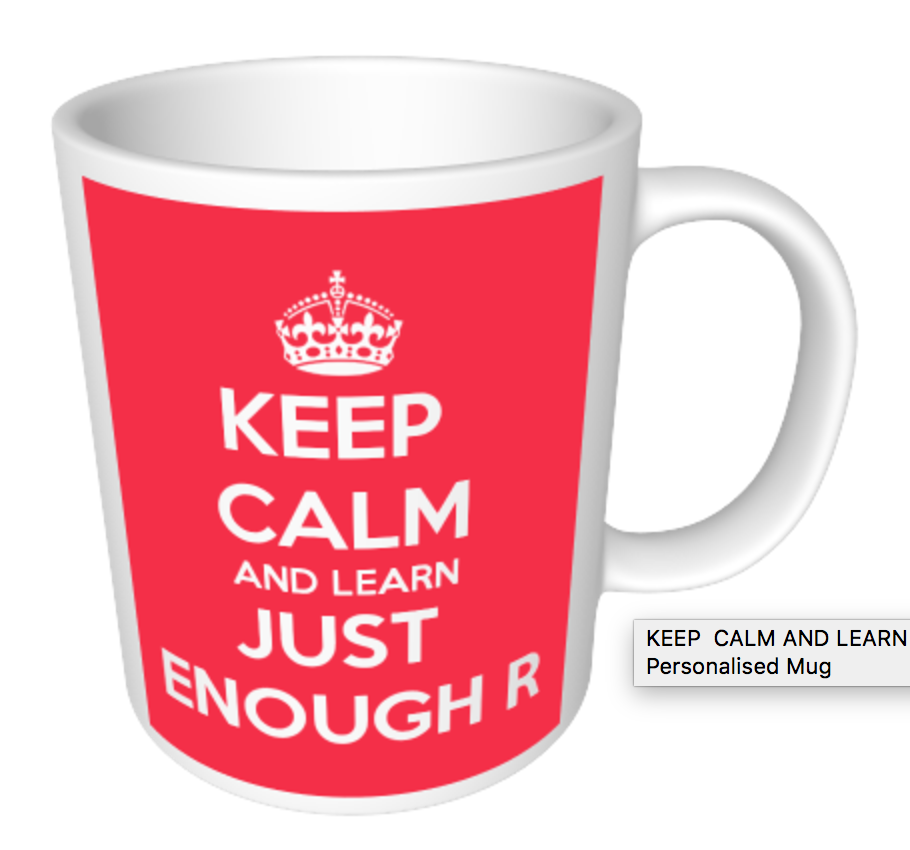
\includegraphics{media/keepcalm.png}
\caption{}
\end{figure}

\section*{Introduction}\label{introduction}
\addcontentsline{toc}{section}{Introduction}

R makes it easy to work with and learn from data.

It also happens to be a complete programmming language, but if you're
reading this guide then that might not be of interest to you. That's OK
--- the goal here is \emph{not} to teach you how to program in
R\footnote{This is actually a lie, but I'm hoping you won't notice until
  it's too late.}. The goal is to teach you \emph{just enough R} to be
confident to explore your data.

In this guide, we use R in the same way we use any other statistics
software: To check and visualise data, run statistical analyses, and
share our results with others. To do that it's worth learning the
\emph{absolute basics} of the R language. The next few chapters walk you
through those basics: what you need to know to be productive in R and
RStudio.

By analogy, imagine going on holiday and learning enough French to
introduce yourself, count from one to ten, and order a baguette. You
won't be fluent - but you won't starve, and your trip will be more fun.

\paragraph{A warning}\label{a-warning}
\addcontentsline{toc}{paragraph}{A warning}

This guide is extremely opinionated.

There are many ways to get things done with R, but trying to learn them
all at once causes unhappiness. In particular, lots of the base R
functions are old, quirky, inconstently named, and hard to remember.
This guide recommends that you use several new `packages' that replicate
and extend some of R's basic functionality.

Using this new set of packages, which are very thoughtfully designed and
work together nicely, will help you form a more consistent mental model
and workflow in R. You can learn the crufty old bits (which do still
have their uses) later on.

The guide also assumes you are using the
\protect\hyperlink{rstudio}{RStudio editor} and working in an
\protect\hyperlink{rmarkdown}{RMarkdown document} (see the next
section). This is important because this guide itself is written in
RMarkdown, and editing it will be an important part of the learning
process. If you don't have access to RStudio yet, see the
\href{installation.html}{installation guide}.

\paragraph{License}\label{license}
\addcontentsline{toc}{paragraph}{License}

These documents are licensed under the
\href{https://creativecommons.org/licenses/by-sa/4.0/}{CC BY-SA
licence}.

\section{Working with R}\label{r-basics}

\subsubsection*{Workflow}\label{start-here}
\addcontentsline{toc}{subsubsection}{Workflow}

One of the biggest adjustments people need to make when moving away from
SPSS or other tools is to work out a `way of working'. Good students
often develop ways of working, saving and communicating their findings
that become habitual. These habits are often attempts to work around
limitations of these packages, so hopefully they will fade in time. But
nevertheless habits are easier to replace than break, so here's an
alternative model to adopt:

\begin{enumerate}
\def\labelenumi{\arabic{enumi}.}
\item
  Work in RStudio, and specifically use RMarkdown documents (see
  \protect\hyperlink{rmarkdown}{next section})
\item
  Always keep your raw data in \protect\hyperlink{use-csv}{.csv format}.
\item
  Avoid saving multiple `processed' versions of your data, and never
  edit data by hand unless absolutely necessary.
\item
  \protect\hyperlink{save-intermediate-steps}{Use R to process data and
  RMarkdown to document the steps taken}.
\item
  `Knit' (run) your RMarkdown documents for sharing with colleagues, or
  for publication.
\end{enumerate}

\hypertarget{rmarkdown}{\subsection*{RMarkdown}\label{rmarkdown}}
\addcontentsline{toc}{subsection}{RMarkdown}

A major weakness of traditional GUI stats packages is that there is no
simple way to document and share your analyses, and so repeating or
editing your work later is very hard.

RMarkdown is a format for documenting and sharing statistical analyses,
and is one of the first things we learn in this guide. This it might
seem an odd place to start the guide: we haven't got anything to share
yet! But RMarkdown provides a really nice way to work with data
interactively, and share results, and so it's worth starting as we mean
to go on.

You are currently reading the output of an `RMarkdown' document.

\begin{itemize}
\tightlist
\item
  R is a computer language designed for working with data.
\item
  Markdown is a simple text-based format which can include prose,
  hypertext links, images, and code (see
  \url{http://commonmark.org/help/}).
\end{itemize}

An RMarkdown document mixes R code with Markdown. This means you can
combine your analysis with text that explains and interprets it.
RMarkdown includes all the details neeed to reproduce an analysis.

Like computer code, RMarkdown can be `run' or `executed'. But in the
language of RStudio, you `knit' your RMarkdown to produce a finished
document. This combines analyses, graphs, and explanatory text in a
single pdf, html, or Word document which can be shared.

\paragraph{\texorpdfstring{Writing and `knitting'
RMarkdown}{Writing and knitting RMarkdown}}\label{writing-and-knitting-rmarkdown}
\addcontentsline{toc}{paragraph}{Writing and `knitting' RMarkdown}

To include R code within RMarkdown we write 3 backticks
(\texttt{\textasciigrave{}\textasciigrave{}\textasciigrave{}}), followed
by \texttt{\{r\}}. We the include our R code, and close the block with 3
more backticks (\protect\hyperlink{backtick-location}{how to find the
backtick on your keyboard}).

\begin{figure}
\centering
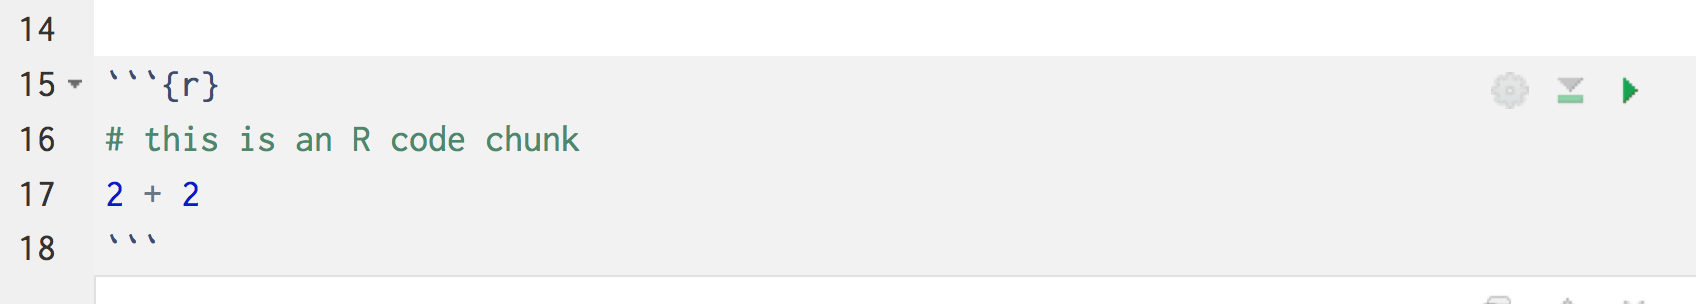
\includegraphics{media/r-code-chunk.png}
\caption{A code chunk in the RMarkdown editor}
\end{figure}

When a document including this chunk is run or `knitted', the final
result will include the the line \texttt{2+2} followed by the number
\texttt{4} on the next line. We can use RMarkdown to `show our
workings': our analysis can be interleaved with narrative text to
explain or interpret the calculations.

\hypertarget{rstudio}{\subsection*{RStudio}\label{rstudio}}
\addcontentsline{toc}{subsection}{RStudio}

RStudio is a text editor which has been customised to make working with
R easy. It can be installed on your own computer, or you can login to a
shared RStudio server (for example, one run by your university) from a
web browser. Either way the interface is largely the same and contains 4
main panels:

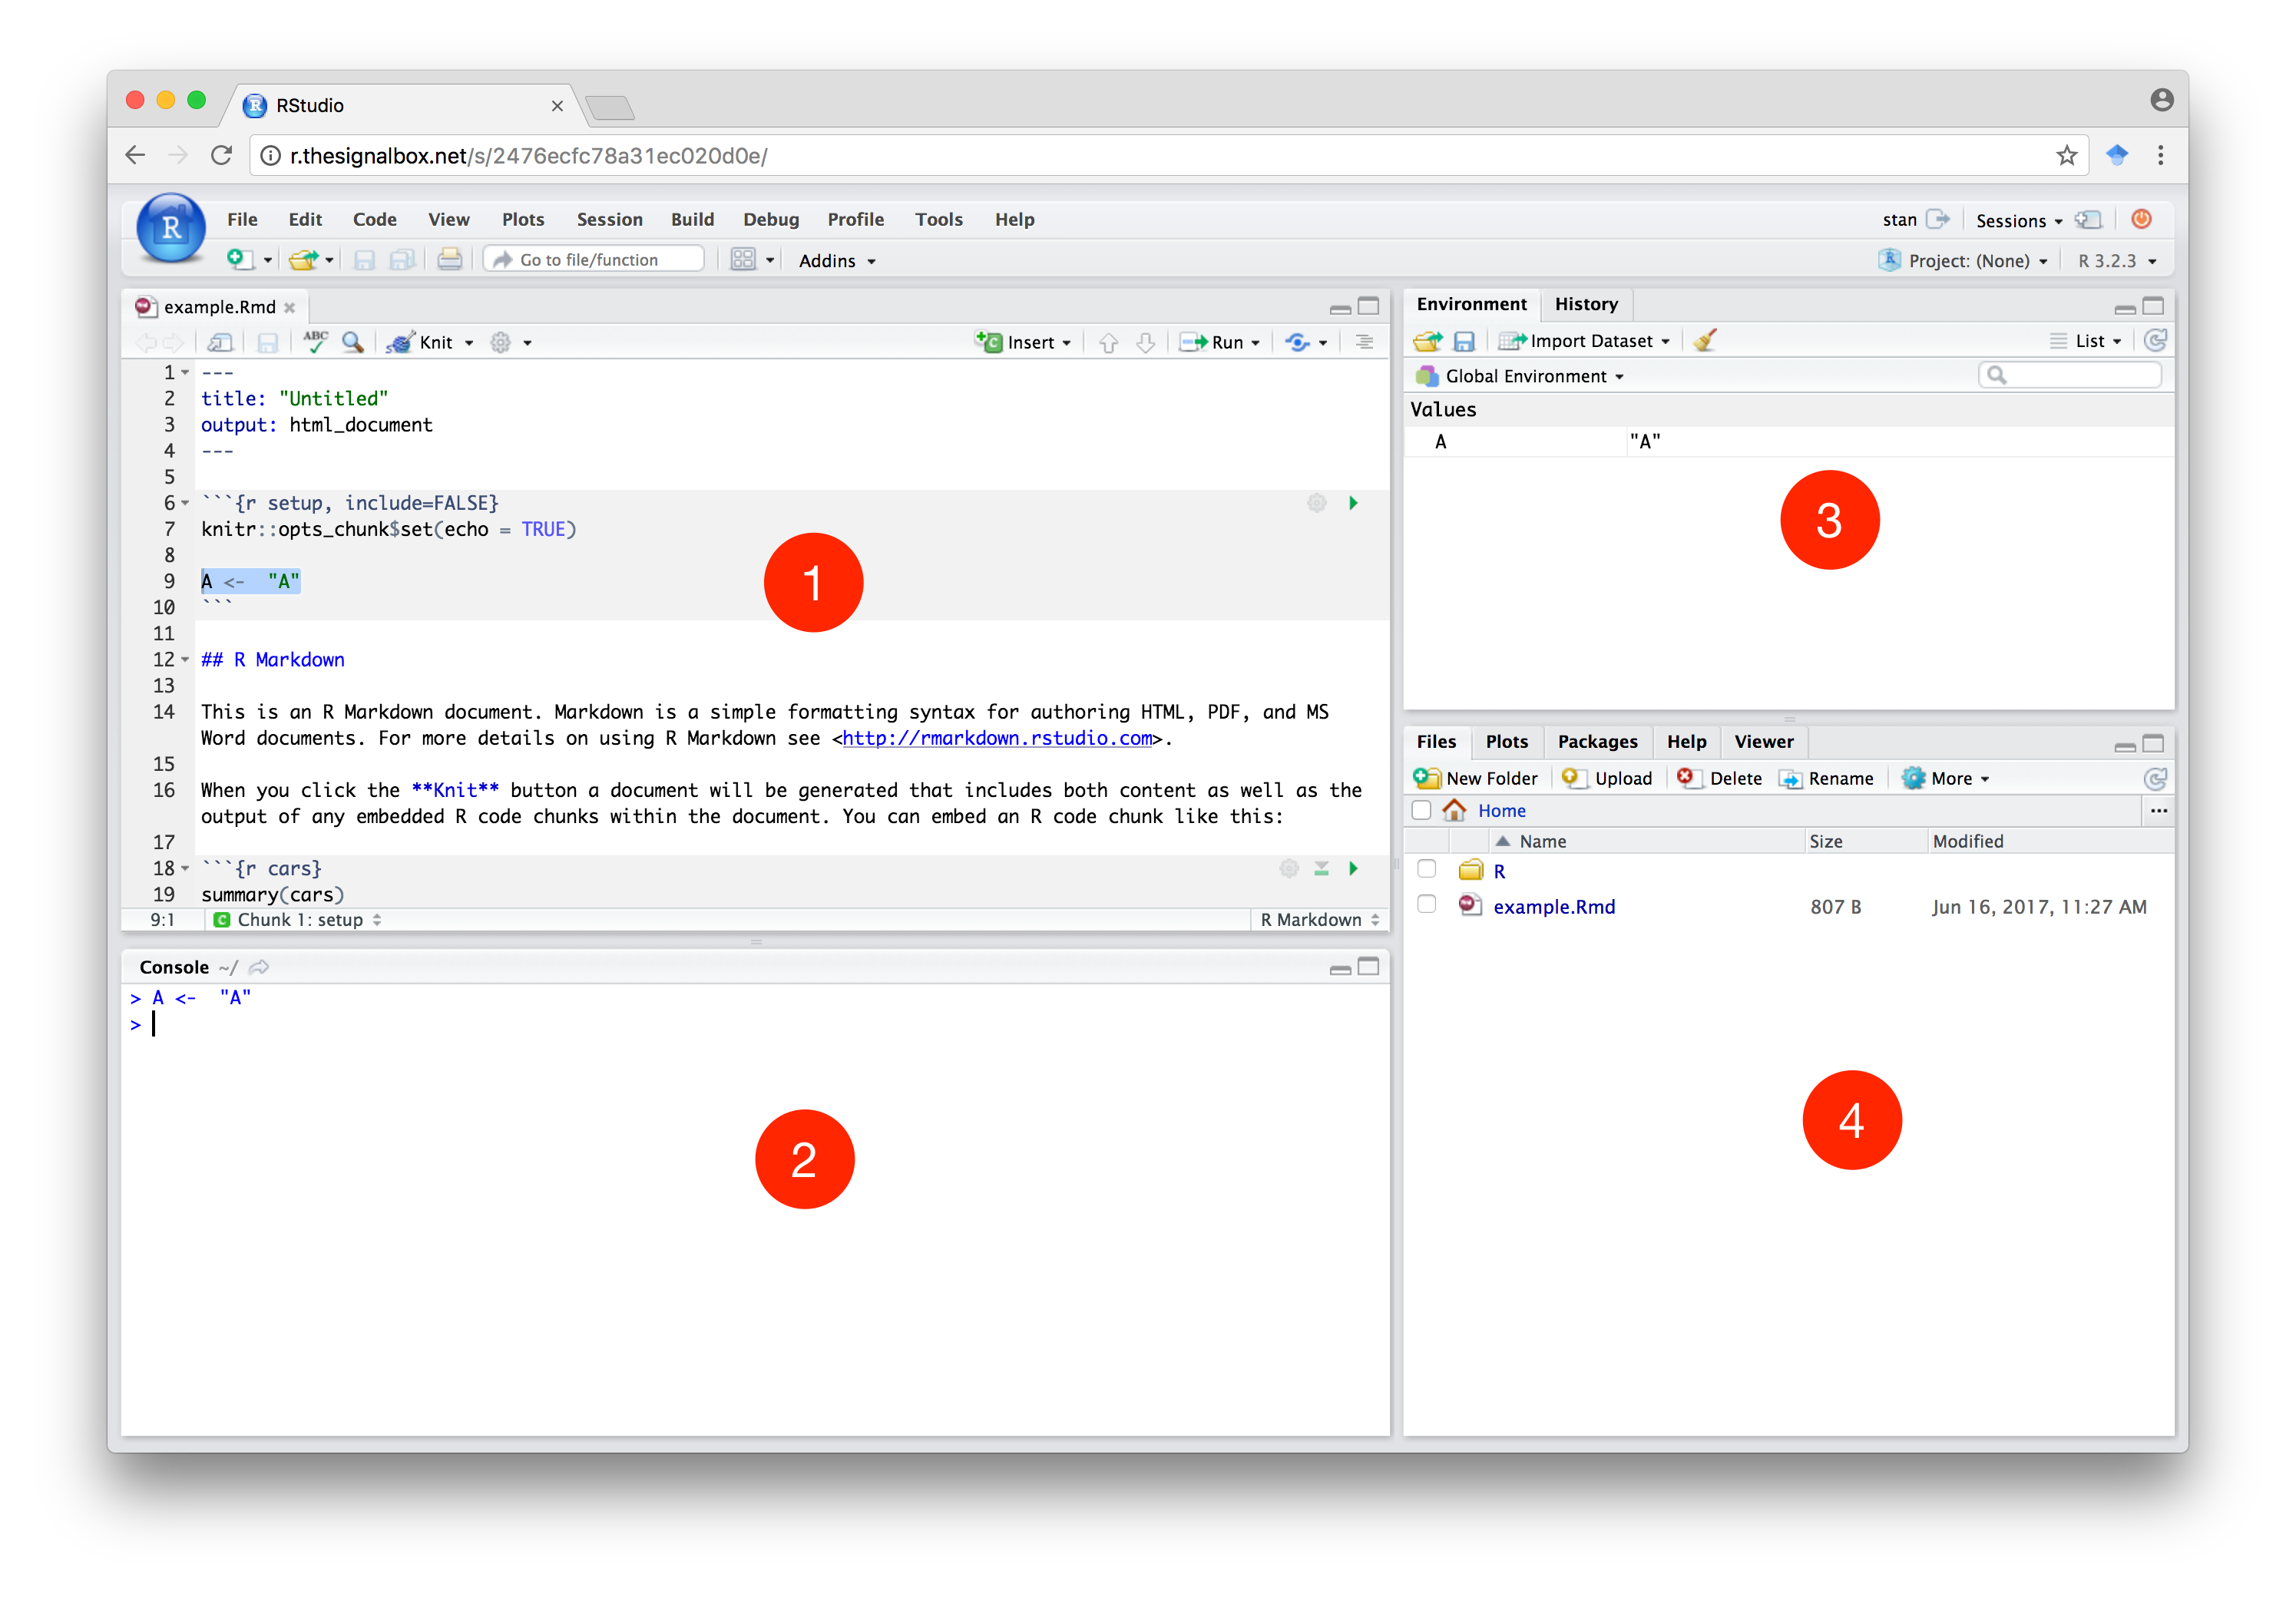
\includegraphics[width=41.53in]{media/rstudio-mainwindow}

The figure above shows the main RStudio interface, comprising:

\begin{enumerate}
\def\labelenumi{\arabic{enumi}.}
\item
  The main R-script or RMarkdown editor window. This is where you write
  commands, which can then be executed (to run the current line type
  ctrl-Enter or cmd-Enter on a Mac).
\item
  The R console, into which you can type R commands directly, and see
  the output of commands run in the script editor.
\item
  The `environment' panel, which lists all the variables you have
  defined and currently available to use.
\item
  The files and help panel. Within this panel the `files' tab enables
  you to open files stored on the server, in the current project, or
  elsewhere on your hard drive.
\end{enumerate}

You can see a short video demonstrating the RStudio interface here:

The video:

\begin{itemize}
\tightlist
\item
  Shows you how to type commands into the Console and view the results.
\item
  Run a plotting function, and see the result.
\item
  Create RMarkdown file, and `Knit' it to produce a document containing
  the results of your code and explanatory text.
\end{itemize}

Once you have watched the video:

\begin{itemize}
\tightlist
\item
  Try creating a new RMarkdown document in RStudio.
\item
  Edit some of the text, and press the Knit button to see the results.
\item
  If you feel brave, edit one of the R blocks and see what happens!
\end{itemize}

More about RMarkdown

A more detailed guide to using RMarkdown, which covers many of the
`chunk options' available to customise output,
\href{http://cfss.uchicago.edu/block013_rmarkdown.html}{is available
here}

If you'd like to use RMarkdown to include manage your citations,
\href{http://rmarkdown.rstudio.com/authoring_bibliographies_and_citations.html}{see
this guide}

\subsection*{First commands}\label{first-commands}
\addcontentsline{toc}{subsection}{First commands}

You can type R commands directly into the console and see the result
there, but you should make a habit of working in an RMarkdown file. This
keeps a record of everything you try, and makes it easy to edit/amend
commands which don't work as you expect.

Now would be a good time to open an RMarkdown document to see how it
works. A good place to start would be to open the source to this
document. The best way to do this is to download the source code for the
`Just Enough R' project, and then open the file
\texttt{start\_here.Rmd}.

\paragraph{}\label{section-1}
\addcontentsline{toc}{paragraph}{}

The source for this RMarkdown file is available here:
\url{https://raw.githubusercontent.com/benwhalley/just-enough-r/master/start_here.Rmd}.

Or you can download the whole project here:
\url{https://github.com/benwhalley/just-enough-r/archive/master.zip}.
This link downloads a `zip' file, which is a compressed folder
containing all the files in the project. To `unzip' it on Mac or Windows
just double-click the file in the Finder or Windows Explorer.

\paragraph{}\label{section-2}
\addcontentsline{toc}{paragraph}{}

To run code in the RStudio interface put your cursor on a line within an
R Block (or select the code you want to run), and press
\texttt{Ctrl-Enter}. The result will appear below the code block.

The command in the R block below prints (shows on screen) the first few
rows of the build-in \texttt{mtcars} example dataset.

Place your cursor somewhere in the line the command is on and run it by
typing \texttt{Ctrl-Enter}, shown in this brief video:

Create an R block in RMarkdown, then run some simple commands.

\begin{Shaded}
\begin{Highlighting}[]
\KeywordTok{head}\NormalTok{(mtcars)}
\NormalTok{##                    mpg cyl disp  hp drat    wt  qsec vs am gear carb}
\NormalTok{## Mazda RX4         21.0   6  160 110 3.90 2.620 16.46  0  1    4    4}
\NormalTok{## Mazda RX4 Wag     21.0   6  160 110 3.90 2.875 17.02  0  1    4    4}
\NormalTok{## Datsun 710        22.8   4  108  93 3.85 2.320 18.61  1  1    4    1}
\NormalTok{## Hornet 4 Drive    21.4   6  258 110 3.08 3.215 19.44  1  0    3    1}
\NormalTok{## Hornet Sportabout 18.7   8  360 175 3.15 3.440 17.02  0  0    3    2}
\NormalTok{## Valiant           18.1   6  225 105 2.76 3.460 20.22  1  0    3    1}
\end{Highlighting}
\end{Shaded}

If you are reading this from within RStudio, running
\texttt{head(mtcars)} will have included an interactive table in the
document, which you can use this to view the \texttt{mtcars} dataset. If
you are still reading the compiled html or pdf document you will see a
table containing the same data, included within the body of the
document.

Hopefully at this point it's obvious that RStudio and RMarkdown give
you:

\begin{itemize}
\tightlist
\item
  A nice place to work with R and explore your data
\item
  A nice format to share your workings (e.g.~with other researchers or
  your tutor)
\item
  A mechanism to save reports of your analysis, to share with other
  people who don't use RStudio
\end{itemize}

\subsection*{Naming things}\label{variables}
\addcontentsline{toc}{subsection}{Naming things}

We can assign labels to the results of calculations and other parts of
our analyses to keep track of them.

To assign labels we use the \texttt{\textless{}-} symbol. The
\texttt{\textless{}-} symbol points from the value we want to store, to
the name we want to use. For example:

\begin{Shaded}
\begin{Highlighting}[]
\NormalTok{the_magic_number <-}\StringTok{ }\DecValTok{3}
\end{Highlighting}
\end{Shaded}

This assigns the value \texttt{3} to the variable
\texttt{the\_magic\_number}. This block wouldn't display anything
because assigning a variable doesn't create any output. To both assign a
variable \emph{and} display it we would type:

\begin{Shaded}
\begin{Highlighting}[]
\NormalTok{the_magic_number <-}\StringTok{ }\DecValTok{3}
\NormalTok{the_magic_number}
\NormalTok{## [1] 3}
\end{Highlighting}
\end{Shaded}

Or we can use a shortcut: if we wrap the line in parentheses this both
makes the assignment and prints the result to the console:

\begin{Shaded}
\begin{Highlighting}[]
\NormalTok{(i_am_a_new_variable <-}\StringTok{ }\DecValTok{22}\NormalTok{)}
\NormalTok{## [1] 22}
\end{Highlighting}
\end{Shaded}

Helpfully, we can do calculations as we assign variables:

\begin{Shaded}
\begin{Highlighting}[]
\NormalTok{one_score <-}\StringTok{ }\DecValTok{20}
\NormalTok{(four_score_years_and_ten <-}\StringTok{ }\NormalTok{one_score }\OperatorTok{*}\StringTok{ }\DecValTok{4} \OperatorTok{+}\StringTok{ }\DecValTok{10}\NormalTok{)}
\NormalTok{## [1] 90}
\end{Highlighting}
\end{Shaded}

{We can give \emph{anything} a label by assigning it to a variable. It
doesn't have to be a number: we can also assign words, graphics and
plots, the results of a statistical model, or \emph{lists} of any of
these things.}

\hypertarget{vectors-and-lists}{\subsection*{Vectors and
lists}\label{vectors-and-lists}}
\addcontentsline{toc}{subsection}{Vectors and lists}

When working with data, we often have lists or sequences of `things'.
For example: a list of measurements we have made.

\begin{itemize}
\item
  When all the things are of the same type, R calls this a
  \emph{vector}\footnote{It's actually a matrix if has 2 dimensions,
    like a table, or an array if it has more than 2 dimensions.}.
\item
  When there is a mix of different things R calls this a \emph{list}.
\end{itemize}

\subsubsection*{Vectors}\label{vector}
\addcontentsline{toc}{subsubsection}{Vectors}

We can create a vector of numbers and display it like this:

\begin{Shaded}
\begin{Highlighting}[]
\CommentTok{# this creates a vector of heights, in cm}
\NormalTok{heights <-}\StringTok{ }\KeywordTok{c}\NormalTok{(}\DecValTok{203}\NormalTok{, }\DecValTok{148}\NormalTok{, }\DecValTok{156}\NormalTok{, }\DecValTok{158}\NormalTok{, }\DecValTok{167}\NormalTok{, }
             \DecValTok{162}\NormalTok{, }\DecValTok{172}\NormalTok{, }\DecValTok{164}\NormalTok{, }\DecValTok{172}\NormalTok{, }\DecValTok{187}\NormalTok{, }
             \DecValTok{134}\NormalTok{, }\DecValTok{182}\NormalTok{, }\DecValTok{175}\NormalTok{)}
\end{Highlighting}
\end{Shaded}

The \texttt{c()} command is shorthand for \emph{combine}, so the example
above combines the individual elements (numbers) into a new vector.

We can create a vector of alphanumeric names just as easily:

\begin{Shaded}
\begin{Highlighting}[]
\NormalTok{names <-}\StringTok{ }\KeywordTok{c}\NormalTok{(}\StringTok{"Ben"}\NormalTok{, }\StringTok{"Joe"}\NormalTok{, }\StringTok{"Sue"}\NormalTok{, }\StringTok{"Rosa"}\NormalTok{)}
\end{Highlighting}
\end{Shaded}

And we can check the values stored in these variables by printing them.
You can either type \texttt{print(heights)}, or just write the name of
the variable alone, which will print it by default. E.g.:

\begin{Shaded}
\begin{Highlighting}[]
\NormalTok{heights }
\NormalTok{##  [1] 203 148 156 158 167 162 172 164 172 187 134 182 175}
\end{Highlighting}
\end{Shaded}

\paragraph{}\label{section-3}
\addcontentsline{toc}{paragraph}{}

Try creating your own vector of numbers in a new code block
below\footnote{i.e.~edit the RMarkdown document} using the
\texttt{c(...)} command. Then change the name of the variable you assign
it to.

\hypertarget{access-vector-elements}{\subsubsection*{Accessing
elements}\label{access-vector-elements}}
\addcontentsline{toc}{subsubsection}{Accessing elements}

Once we have created a vector, we often want to access the individual
elements again. We do this based on their \emph{position}.

Let's say we have created a vector:

\begin{Shaded}
\begin{Highlighting}[]
\NormalTok{my.vector <-}\StringTok{ }\KeywordTok{c}\NormalTok{(}\DecValTok{10}\NormalTok{, }\DecValTok{20}\NormalTok{, }\DecValTok{30}\NormalTok{, }\DecValTok{40}\NormalTok{)}
\end{Highlighting}
\end{Shaded}

We can display the whole vector by just typing its name, as we saw
above. But if we want to show only the \emph{first} element of this
vector, we type:

\begin{Shaded}
\begin{Highlighting}[]
\NormalTok{my.vector[}\DecValTok{1}\NormalTok{]}
\NormalTok{## [1] 10}
\end{Highlighting}
\end{Shaded}

Here, the square brackets specify a \emph{subset} of the vector we want
- in this case, just the first element.

\subsubsection*{Selecting more than one
element}\label{selecting-more-than-one-element}
\addcontentsline{toc}{subsubsection}{Selecting more than one element}

A neat feature of subsetting is that we can grab more than one element
at a time.

To do this, we need to tell R the \emph{positions} of the elements we
want, and so we provide a \emph{vector of the positions of the elements
we want}.

It might seem obvious, but the first element has position 1, the second
has position 2, and so on. So, if we wanted to extract the 4th and 5th
elements from the vector of heights we saw above we would type:

\begin{Shaded}
\begin{Highlighting}[]
\NormalTok{elements.to.grab <-}\StringTok{ }\KeywordTok{c}\NormalTok{(}\DecValTok{4}\NormalTok{, }\DecValTok{5}\NormalTok{)}
\NormalTok{heights[elements.to.grab]}
\NormalTok{## [1] 158 167}
\end{Highlighting}
\end{Shaded}

We can also make a subset of the original vector and assign it to a
\emph{new} variable:

\begin{Shaded}
\begin{Highlighting}[]
\NormalTok{first.two.elements <-}\StringTok{ }\NormalTok{heights[}\KeywordTok{c}\NormalTok{(}\DecValTok{1}\NormalTok{, }\DecValTok{2}\NormalTok{)]}
\NormalTok{first.two.elements}
\NormalTok{## [1] 203 148}
\end{Highlighting}
\end{Shaded}

\subsection*{Processing vectors}\label{processing-vectors}
\addcontentsline{toc}{subsection}{Processing vectors}

Many of R's most useful functions process \emph{vectors of numbers} in
some way. For example, if we want to calculate the average of our vector
of heights we just type:

\begin{Shaded}
\begin{Highlighting}[]
\KeywordTok{mean}\NormalTok{(heights)}
\NormalTok{## [1] 167.6923}
\end{Highlighting}
\end{Shaded}

R contains \emph{lots} of built in functions which we can use to
summarise a vector of numbers. For example:

\begin{Shaded}
\begin{Highlighting}[]
\KeywordTok{median}\NormalTok{(heights)}
\NormalTok{## [1] 167}
\KeywordTok{sd}\NormalTok{(heights)}
\NormalTok{## [1] 17.59443}
\KeywordTok{min}\NormalTok{(heights)}
\NormalTok{## [1] 134}
\KeywordTok{max}\NormalTok{(heights)}
\NormalTok{## [1] 203}
\KeywordTok{range}\NormalTok{(heights)}
\NormalTok{## [1] 134 203}
\KeywordTok{IQR}\NormalTok{(heights)}
\NormalTok{## [1] 17}
\KeywordTok{length}\NormalTok{(heights)}
\NormalTok{## [1] 13}
\end{Highlighting}
\end{Shaded}

All of these functions accept a vector as input, do some proccesing, and
then return a \emph{single number} which gets displayed by RStudio.

But not all functions return a single number in the way that
\texttt{mean} did above. Some return a new vector, or some other type of
object instead. For example, the \texttt{quantile} function returns the
values at the 0, 25th, 50th, 75th and 100th percentiles (by default).

\begin{Shaded}
\begin{Highlighting}[]
\NormalTok{height.quantiles <-}\StringTok{ }\KeywordTok{quantile}\NormalTok{(heights)}
\NormalTok{height.quantiles}
\NormalTok{##   0%  25%  50%  75% 100% }
\NormalTok{##  134  158  167  175  203}
\end{Highlighting}
\end{Shaded}

If a function returns a vector, we can use it just like any other
vector:

\begin{Shaded}
\begin{Highlighting}[]
\NormalTok{height.quantiles <-}\StringTok{ }\KeywordTok{quantile}\NormalTok{(heights)}

\CommentTok{# grab the third element, which is the median}
\NormalTok{height.quantiles[}\DecValTok{3}\NormalTok{]}
\NormalTok{## 50% }
\NormalTok{## 167}

\CommentTok{# assign the first element to a variable}
\NormalTok{min.height <-}\StringTok{ }\NormalTok{height.quantiles[}\DecValTok{1}\NormalTok{]}
\NormalTok{min.height}
\NormalTok{##  0% }
\NormalTok{## 134}
\end{Highlighting}
\end{Shaded}

But other functions process a vector without returning any numbers. For
example, the \texttt{hist} function returns a histogram:

\begin{Shaded}
\begin{Highlighting}[]
\KeywordTok{hist}\NormalTok{(heights)}
\end{Highlighting}
\end{Shaded}

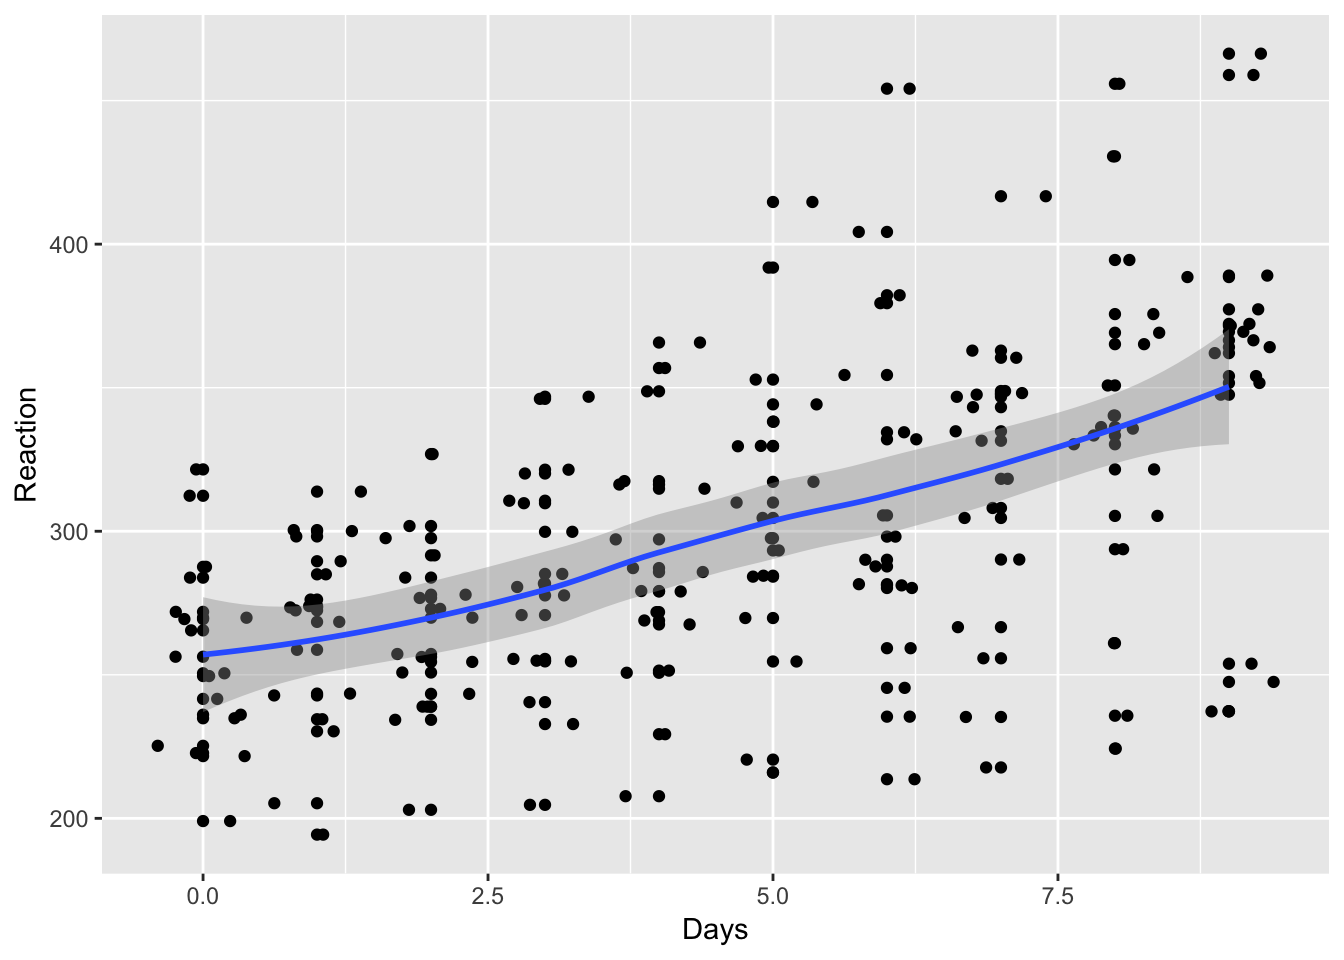
\includegraphics{start_here_files/figure-latex/unnamed-chunk-19-1.pdf}

We'll cover lots more plotting and visualisation later on.

\subsubsection*{Making new vectors}\label{making-new-vectors}
\addcontentsline{toc}{subsubsection}{Making new vectors}

So far we've seen R functions which process a vector of numbers and
produce a single number, a new vector of a different length (like
\texttt{quantile} or \texttt{fivenum}), or some other object (like
\texttt{hist} which makes a plot). However many other functions accept a
single input, do something to it, and return a single processed value.

For example, the square root function, \texttt{sqrt}, accepts a single
value and returns a single value: running \texttt{sqrt(10)} will return
\texttt{3.1623}.

In R, if a function accepts a single value as input and returns a single
value as output (like \texttt{sqrt(10)}), then you can usually give a
vector as input too. Some people find this surprising\footnote{Mostly
  people who already know other programming languages like C. It's not
  that surprising if you read the R code as you would English.}, but R
assumes that if you're processing a vector of numbers, you want the
function applied to each of them in the same way.

This turns out to be very useful. For example, let's say we want the
square root of each of the elements of our height data:

\begin{Shaded}
\begin{Highlighting}[]
\CommentTok{# these are the raw values}
\NormalTok{heights}
\NormalTok{##  [1] 203 148 156 158 167 162 172 164 172 187 134 182 175}

\CommentTok{# takes the sqrt of each value and returns a vector of all the square roots}
\KeywordTok{sqrt}\NormalTok{(heights)}
\NormalTok{##  [1] 14.24781 12.16553 12.49000 12.56981 12.92285 12.72792 13.11488}
\NormalTok{##  [8] 12.80625 13.11488 13.67479 11.57584 13.49074 13.22876}
\end{Highlighting}
\end{Shaded}

This also works with simple arithmetic So, if we wanted to convert all
the heights from cm to meters we could just type:

\begin{Shaded}
\begin{Highlighting}[]
\NormalTok{heights }\OperatorTok{/}\StringTok{ }\DecValTok{100}
\NormalTok{##  [1] 2.03 1.48 1.56 1.58 1.67 1.62 1.72 1.64 1.72 1.87 1.34 1.82 1.75}
\end{Highlighting}
\end{Shaded}

\hypertarget{paste}{\paragraph{}\label{paste}}
\addcontentsline{toc}{paragraph}{}

This trick also works with other functions like \texttt{paste}, which
combines the inputs you send it to produce an alphanumeric string:

\begin{Shaded}
\begin{Highlighting}[]
\KeywordTok{paste}\NormalTok{(}\StringTok{"Once"}\NormalTok{, }\StringTok{"upon"}\NormalTok{, }\StringTok{"a"}\NormalTok{, }\StringTok{"time"}\NormalTok{)}
\NormalTok{## [1] "Once upon a time"}
\end{Highlighting}
\end{Shaded}

If we send a vector to \texttt{paste} it assumes we want a vector of
results, with each element in the vector pasted next to each other:

\begin{Shaded}
\begin{Highlighting}[]
\NormalTok{bottles <-}\StringTok{ }\KeywordTok{c}\NormalTok{(}\DecValTok{100}\NormalTok{, }\DecValTok{99}\NormalTok{, }\DecValTok{98}\NormalTok{, }\StringTok{"..."}\NormalTok{)}
\KeywordTok{paste}\NormalTok{(bottles, }\StringTok{"green bottles hanging on the wall"}\NormalTok{)}
\NormalTok{## [1] "100 green bottles hanging on the wall"}
\NormalTok{## [2] "99 green bottles hanging on the wall" }
\NormalTok{## [3] "98 green bottles hanging on the wall" }
\NormalTok{## [4] "... green bottles hanging on the wall"}
\end{Highlighting}
\end{Shaded}

In other programming languages we might have had to write a `loop' to
create each line of the song, but R lets us write short statements to
summarise \emph{what} needs to be done; we don't need to worry worrying
about \emph{how} it gets done.

\paragraph{}\label{paste0}
\addcontentsline{toc}{paragraph}{}

The \texttt{paste0} function does much the same, but leaves no spaces in
the combined strings, which can be useful:

\begin{Shaded}
\begin{Highlighting}[]
\KeywordTok{paste0}\NormalTok{(}\StringTok{"N="}\NormalTok{, }\DecValTok{1}\OperatorTok{:}\DecValTok{10}\NormalTok{)}
\NormalTok{##  [1] "N=1"  "N=2"  "N=3"  "N=4"  "N=5"  "N=6"  "N=7"  "N=8"  "N=9"  "N=10"}
\end{Highlighting}
\end{Shaded}

\subsubsection*{Making up data (new
vectors)}\label{making-up-data-new-vectors}
\addcontentsline{toc}{subsubsection}{Making up data (new vectors)}

Sometimes you'll need to create vectors containing regular sequences or
randomly selected numbers.

To create regular sequences a convenient shortcut is the `colon'
operator. For example, if we type \texttt{1:10} then we get a vector of
numbers from 1 to 10:

\begin{Shaded}
\begin{Highlighting}[]
\DecValTok{1}\OperatorTok{:}\DecValTok{10}
\NormalTok{##  [1]  1  2  3  4  5  6  7  8  9 10}
\end{Highlighting}
\end{Shaded}

The \texttt{seq} function allows you to create more specific sequences:

\begin{Shaded}
\begin{Highlighting}[]
\CommentTok{# make a sequence, specifying the interval between them}
\KeywordTok{seq}\NormalTok{(}\DataTypeTok{from=}\FloatTok{0.1}\NormalTok{, }\DataTypeTok{to=}\DecValTok{2}\NormalTok{, }\DataTypeTok{by=}\NormalTok{.}\DecValTok{1}\NormalTok{)}
\NormalTok{##  [1] 0.1 0.2 0.3 0.4 0.5 0.6 0.7 0.8 0.9 1.0 1.1 1.2 1.3 1.4 1.5 1.6 1.7}
\NormalTok{## [18] 1.8 1.9 2.0}
\end{Highlighting}
\end{Shaded}

We can also use random number-generating functions built into R to
create vectors:

\begin{Shaded}
\begin{Highlighting}[]
\CommentTok{# 10 uniformly distributed random numbers between 0 and 1}
\KeywordTok{runif}\NormalTok{(}\DecValTok{10}\NormalTok{)}
\NormalTok{##  [1] 0.4045490 0.5345472 0.4414659 0.4832063 0.2562126 0.2040762 0.6876566}
\NormalTok{##  [8] 0.4578561 0.1847851 0.8843672}

\CommentTok{# 1,000 uniformly distributed random numbers between 1 and 100}
\NormalTok{my.numbers <-}\StringTok{ }\KeywordTok{runif}\NormalTok{(}\DecValTok{1000}\NormalTok{, }\DecValTok{1}\NormalTok{, }\DecValTok{10}\NormalTok{)}

\CommentTok{# 10 random-normal numbers with mean 10 and SD=1}
\KeywordTok{rnorm}\NormalTok{(}\DecValTok{10}\NormalTok{, }\DataTypeTok{mean=}\DecValTok{10}\NormalTok{)}
\NormalTok{##  [1] 11.342605 11.115379  9.036358  9.062017 10.748910  9.390587 10.194291}
\NormalTok{##  [8] 10.306759 10.127122  8.247792}

\CommentTok{# 10 random-normal numbers with mean 10 and SD=5}
\KeywordTok{rnorm}\NormalTok{(}\DecValTok{10}\NormalTok{, }\DecValTok{10}\NormalTok{, }\DecValTok{5}\NormalTok{)}
\NormalTok{##  [1]  7.9126611 14.3523243 22.7525075 11.2225728  1.9833647 13.1075665}
\NormalTok{##  [7]  6.0708431  9.4363061  0.2478268 11.1413276}
\end{Highlighting}
\end{Shaded}

We can then use these numbers in our code, for example plotting them:

\begin{Shaded}
\begin{Highlighting}[]
\NormalTok{random.numbers <-}\StringTok{ }\KeywordTok{rnorm}\NormalTok{(}\DecValTok{10000}\NormalTok{)}
\KeywordTok{hist}\NormalTok{(random.numbers)}
\end{Highlighting}
\end{Shaded}

\includegraphics{start_here_files/figure-latex/unnamed-chunk-28-1.pdf}

\subsection*{Functions to learn now}\label{functions-to-learn-now}
\addcontentsline{toc}{subsection}{Functions to learn now}

There are \emph{thousands} of functions built into R. Below are just a
few examples which are likely to be useful as you work with your data:

Repetition

\begin{Shaded}
\begin{Highlighting}[]
\CommentTok{# repeat something N times}
\KeywordTok{rep}\NormalTok{(}\StringTok{"Apple pie"}\NormalTok{, }\DecValTok{10}\NormalTok{)}
\NormalTok{##  [1] "Apple pie" "Apple pie" "Apple pie" "Apple pie" "Apple pie"}
\NormalTok{##  [6] "Apple pie" "Apple pie" "Apple pie" "Apple pie" "Apple pie"}
\end{Highlighting}
\end{Shaded}

\begin{Shaded}
\begin{Highlighting}[]
\CommentTok{# repeat a short vector, combining into a single longer vector}
\KeywordTok{rep}\NormalTok{(}\KeywordTok{c}\NormalTok{(}\StringTok{"Custard"}\NormalTok{, }\StringTok{"Gravy"}\NormalTok{), }\DecValTok{5}\NormalTok{)}
\NormalTok{##  [1] "Custard" "Gravy"   "Custard" "Gravy"   "Custard" "Gravy"   "Custard"}
\NormalTok{##  [8] "Gravy"   "Custard" "Gravy"}
\end{Highlighting}
\end{Shaded}

Sequences

\begin{Shaded}
\begin{Highlighting}[]
\CommentTok{# make a sequence }
\NormalTok{(countdown <-}\StringTok{ }\DecValTok{100}\OperatorTok{:}\DecValTok{1}\NormalTok{)}
\NormalTok{##   [1] 100  99  98  97  96  95  94  93  92  91  90  89  88  87  86  85  84}
\NormalTok{##  [18]  83  82  81  80  79  78  77  76  75  74  73  72  71  70  69  68  67}
\NormalTok{##  [35]  66  65  64  63  62  61  60  59  58  57  56  55  54  53  52  51  50}
\NormalTok{##  [52]  49  48  47  46  45  44  43  42  41  40  39  38  37  36  35  34  33}
\NormalTok{##  [69]  32  31  30  29  28  27  26  25  24  23  22  21  20  19  18  17  16}
\NormalTok{##  [86]  15  14  13  12  11  10   9   8   7   6   5   4   3   2   1}
\end{Highlighting}
\end{Shaded}

Make sequences with steps of a particular size:

\begin{Shaded}
\begin{Highlighting}[]
\NormalTok{(tenths  <-}\StringTok{ }\KeywordTok{seq}\NormalTok{(}\DataTypeTok{from=}\DecValTok{0}\NormalTok{, }\DataTypeTok{to=}\DecValTok{1}\NormalTok{, }\DataTypeTok{by=}\NormalTok{.}\DecValTok{1}\NormalTok{))}
\NormalTok{##  [1] 0.0 0.1 0.2 0.3 0.4 0.5 0.6 0.7 0.8 0.9 1.0}

\NormalTok{(twelfths <-}\StringTok{ }\KeywordTok{seq}\NormalTok{(}\DataTypeTok{from=}\DecValTok{0}\NormalTok{, }\DataTypeTok{to=}\DecValTok{10}\NormalTok{, }\DataTypeTok{length.out=}\DecValTok{12}\NormalTok{))}
\NormalTok{##  [1]  0.0000000  0.9090909  1.8181818  2.7272727  3.6363636  4.5454545}
\NormalTok{##  [7]  5.4545455  6.3636364  7.2727273  8.1818182  9.0909091 10.0000000}
\end{Highlighting}
\end{Shaded}

Ranking

\begin{Shaded}
\begin{Highlighting}[]
\CommentTok{# generate some random data (here, ages in years)}
\NormalTok{ages <-}\StringTok{ }\KeywordTok{round}\NormalTok{(}\KeywordTok{rnorm}\NormalTok{(}\DecValTok{10}\NormalTok{, }\DataTypeTok{mean=}\DecValTok{40}\NormalTok{, }\DataTypeTok{sd=}\DecValTok{10}\NormalTok{))}

\CommentTok{# get the rank order of elements (i.e. what their positions would be if the vector was sorted)}
\NormalTok{ages}
\NormalTok{##  [1] 39 32 36 27 26 11 21 38 40 47}
\KeywordTok{rank}\NormalTok{(ages, }\DataTypeTok{ties.method=}\StringTok{"first"}\NormalTok{)}
\NormalTok{##  [1]  8  5  6  4  3  1  2  7  9 10}
\end{Highlighting}
\end{Shaded}

Unique values

\begin{Shaded}
\begin{Highlighting}[]
\CommentTok{# return the unique values in a vector}
\KeywordTok{unique}\NormalTok{(}\KeywordTok{rep}\NormalTok{(}\DecValTok{1}\OperatorTok{:}\DecValTok{10}\NormalTok{, }\DecValTok{100}\NormalTok{))}
\NormalTok{##  [1]  1  2  3  4  5  6  7  8  9 10}
\end{Highlighting}
\end{Shaded}

Lengths

\begin{Shaded}
\begin{Highlighting}[]
\CommentTok{# return the unique values in a vector}
\KeywordTok{length}\NormalTok{(}\KeywordTok{seq}\NormalTok{(}\DecValTok{1}\NormalTok{,}\DecValTok{100}\NormalTok{, }\DecValTok{2}\NormalTok{))}
\NormalTok{## [1] 50}
\end{Highlighting}
\end{Shaded}

Try and experiment with each of these functions. Check the output
against what you expected to happen, and make sure you understand what
they do.

\hypertarget{lists}{\subsection*{Lists}\label{lists}}
\addcontentsline{toc}{subsection}{Lists}

Try running the code below:

\begin{Shaded}
\begin{Highlighting}[]
\NormalTok{(confusing.vector <-}\StringTok{ }\KeywordTok{c}\NormalTok{(}\DecValTok{1}\NormalTok{, }\DecValTok{2}\NormalTok{, }\DecValTok{3}\NormalTok{, }\StringTok{"Wibble"}\NormalTok{))}
\NormalTok{## [1] "1"      "2"      "3"      "Wibble"}
\NormalTok{(first.element <-}\StringTok{ }\NormalTok{confusing.vector[}\DecValTok{1}\NormalTok{])}
\NormalTok{## [1] "1"}
\KeywordTok{sqrt}\NormalTok{(first.element)}
\NormalTok{## Error in sqrt(first.element): non-numeric argument to mathematical function}
\end{Highlighting}
\end{Shaded}

Take a minute to try and make a guess at what went wrong. Why does R
complain that the `\texttt{1}' is non-numeric?

When we built the vector we used \texttt{c} to combine the elements
\texttt{1}, \texttt{2}, \texttt{3} and \texttt{"Wibble"}. Although our
first three elements are numbers, \texttt{"Wibble"} is not - it's made
up of letters (this is called a character string).

Vectors can only contain one \emph{type} of thing so R automatically
converts all the elements to the same type, if it can.

Because R can't reliably convert \texttt{"Wibble"} to a number,
everything in the vector was converted to the \texttt{character} type
instead. We get an error because R can't mutiply words together.

If you're not sure what type of thing your vector contains, you can use
the \texttt{typeof} function:

\begin{Shaded}
\begin{Highlighting}[]
\KeywordTok{typeof}\NormalTok{(}\DecValTok{1}\OperatorTok{:}\DecValTok{10}\NormalTok{)}
\NormalTok{## [1] "integer"}
\KeywordTok{typeof}\NormalTok{(}\KeywordTok{runif}\NormalTok{(}\DecValTok{10}\NormalTok{))}
\NormalTok{## [1] "double"}
\KeywordTok{typeof}\NormalTok{(}\KeywordTok{c}\NormalTok{(}\DecValTok{1}\NormalTok{, }\DecValTok{2}\NormalTok{, }\StringTok{"Wibble"}\NormalTok{))}
\NormalTok{## [1] "character"}
\end{Highlighting}
\end{Shaded}

Here the meaning of \emph{integer} should be self explanatory. The
vector \texttt{runif(10)} has type \emph{double}, because it contains
`double-precision' floating point numbers. For our purposes you can just
think of \texttt{double} as meaning any number with decimal places.

The last vector has the type \texttt{character} because it includes the
character string \texttt{Wibble}, and all the other numbers in it were
coerced to become character strings too.

If we want to (safely) mix up different types of object without them
being converted we need a proper \texttt{list}, rather than a vector. In
R we would write:

\begin{Shaded}
\begin{Highlighting}[]
\NormalTok{my.list <-}\StringTok{ }\KeywordTok{list}\NormalTok{(}\DecValTok{2}\NormalTok{, }\DecValTok{2}\NormalTok{, }\StringTok{"Wibble"}\NormalTok{)}
\end{Highlighting}
\end{Shaded}

We can still access elements from lists as we do for vectors, although
now we need to use double square brackets, for example:

\begin{Shaded}
\begin{Highlighting}[]
\NormalTok{my.list[[}\DecValTok{1}\NormalTok{]]}
\NormalTok{## [1] 2}
\end{Highlighting}
\end{Shaded}

But now our numbers haven't been converted to character strings, and we
can still multiply them.

\begin{Shaded}
\begin{Highlighting}[]
\NormalTok{my.list[[}\DecValTok{1}\NormalTok{]] }\OperatorTok{*}\StringTok{ }\NormalTok{my.list[[}\DecValTok{2}\NormalTok{]]}
\NormalTok{## [1] 4}
\end{Highlighting}
\end{Shaded}

Square brackets are ugly and can be confusing though, so we often give
names to the elements of our list when we create it:

\begin{Shaded}
\begin{Highlighting}[]
\NormalTok{my.party <-}\StringTok{ }\KeywordTok{list}\NormalTok{(}\DataTypeTok{number.guests=}\DecValTok{8}\NormalTok{, }
                 \DataTypeTok{when=}\StringTok{"Friday"}\NormalTok{, }
                 \DataTypeTok{drinks =} \KeywordTok{c}\NormalTok{(}\StringTok{"Juice"}\NormalTok{, }\StringTok{"Beer"}\NormalTok{, }\StringTok{"Whisky"}\NormalTok{))}
\end{Highlighting}
\end{Shaded}

Which means we can then access the elements \emph{by name} later on. To
do this, you write the name of the vector, then a \texttt{\$} sign, and
then the name of the element you want to access:

\begin{Shaded}
\begin{Highlighting}[]
\NormalTok{my.party}\OperatorTok{$}\NormalTok{when}
\NormalTok{## [1] "Friday"}
\end{Highlighting}
\end{Shaded}

You might have spotted that we included a vector inside the party list.
This is not a problem, and we can still access individual elements of
this vector too:

\begin{Shaded}
\begin{Highlighting}[]
\NormalTok{my.party}\OperatorTok{$}\NormalTok{drinks[}\DecValTok{1}\NormalTok{]}
\NormalTok{## [1] "Juice"}
\end{Highlighting}
\end{Shaded}

\paragraph{}\label{section-5}
\addcontentsline{toc}{paragraph}{}

\begin{enumerate}
\def\labelenumi{\arabic{enumi}.}
\tightlist
\item
  Create a vector containing 3 numbers then:
\end{enumerate}

\begin{itemize}
\tightlist
\item
  Access just the last number
\item
  Create a new vector containing just the first and last number
\end{itemize}

\begin{enumerate}
\def\labelenumi{\arabic{enumi}.}
\setcounter{enumi}{1}
\tightlist
\item
  Create a list containing your address and your age in years. Then:
\end{enumerate}

\begin{itemize}
\tightlist
\item
  Multiply your age in years by your flat or house number (by accessing
  the relevant elements in the list)
\end{itemize}

\begin{enumerate}
\def\labelenumi{\arabic{enumi}.}
\setcounter{enumi}{2}
\tightlist
\item
  Run the following R code and explain what has happened:
\end{enumerate}

\begin{Shaded}
\begin{Highlighting}[]
\KeywordTok{sqrt}\NormalTok{(}\DecValTok{1}\OperatorTok{:}\DecValTok{10}\NormalTok{) }\OperatorTok{*}\StringTok{ }\DecValTok{10}
\NormalTok{##  [1] 10.00000 14.14214 17.32051 20.00000 22.36068 24.49490 26.45751}
\NormalTok{##  [8] 28.28427 30.00000 31.62278}
\end{Highlighting}
\end{Shaded}

\paragraph{}\label{section-6}
\addcontentsline{toc}{paragraph}{}

Extended questions:

\begin{itemize}
\item
  What is the average of the 9 times table, up to and including 9 x
  1000?
\item
  Use the \texttt{paste} and \texttt{c(...)} functions to create a
  vector which contains the sequence ``1 elephant'', ``2 elephants'',
  \ldots{}, ``1000 elephants''.
\end{itemize}

\part{Data}\label{data}

\hypertarget{datasets-dataframes}{\section{Datasets and
dataframes}\label{datasets-dataframes}}

A dataframe is an object which can store data as you might encounter it
in SPSS, Stata, or other statistics packages.

It's much like a spreadsheet, but with some constraints applied.
`Constraints' sound bad, but are helpful here: they make dataframes more
structured and predictable to work with:

\begin{itemize}
\item
  Each column is a \protect\hyperlink{vectors-and-lists}{vector}, and so
  can \protect\hyperlink{vectors-and-lists}{only store one type of
  data}.
\item
  Every column has to be the same length (although missing values are
  allowed).
\item
  Each column should have a name.
\end{itemize}

Put another way, a dataframe behaves like a \emph{list} of
\emph{vectors}, which means we can use a lot of the same rules to
\protect\hyperlink{access-vector-elements}{access elements within them}
(more on this below).

\paragraph{\texorpdfstring{Using `built in'
data}{Using built in data}}\label{built-in-data}
\addcontentsline{toc}{paragraph}{Using `built in' data}

The quickest way to see a dataframe in action is to use one that is
\href{https://stat.ethz.ch/R-manual/R-devel/library/datasets/html/00Index.html}{built
in to R}. For example:

\begin{Shaded}
\begin{Highlighting}[]
\KeywordTok{head}\NormalTok{(airquality)}
\NormalTok{##   Ozone Solar.R Wind Temp Month Day}
\NormalTok{## 1    41     190  7.4   67     5   1}
\NormalTok{## 2    36     118  8.0   72     5   2}
\NormalTok{## 3    12     149 12.6   74     5   3}
\NormalTok{## 4    18     313 11.5   62     5   4}
\NormalTok{## 5    NA      NA 14.3   56     5   5}
\NormalTok{## 6    28      NA 14.9   66     5   6}
\end{Highlighting}
\end{Shaded}

Or

\begin{Shaded}
\begin{Highlighting}[]
\KeywordTok{head}\NormalTok{(mtcars)}
\NormalTok{##                    mpg cyl disp  hp drat    wt  qsec vs am gear carb}
\NormalTok{## Mazda RX4         21.0   6  160 110 3.90 2.620 16.46  0  1    4    4}
\NormalTok{## Mazda RX4 Wag     21.0   6  160 110 3.90 2.875 17.02  0  1    4    4}
\NormalTok{## Datsun 710        22.8   4  108  93 3.85 2.320 18.61  1  1    4    1}
\NormalTok{## Hornet 4 Drive    21.4   6  258 110 3.08 3.215 19.44  1  0    3    1}
\NormalTok{## Hornet Sportabout 18.7   8  360 175 3.15 3.440 17.02  0  0    3    2}
\NormalTok{## Valiant           18.1   6  225 105 2.76 3.460 20.22  1  0    3    1}
\end{Highlighting}
\end{Shaded}

In both these examples the datasets (\texttt{airquality} and
\texttt{mtcars}) are already loaded and available to be used in the
\texttt{head()} function.

{To find a list of all the built in datasets you can type
\texttt{help(datasets)} or see
\url{https://stat.ethz.ch/R-manual/R-devel/library/datasets/html/00Index.html}.
Familiarise yourself with some of the other included datasets, e.g.
\texttt{datasets::attitude}. Watch out that not all the included
datasets are \emph{dataframes}: Some are just vectors of observations
(e.g.~the \texttt{airmiles} data) and some are `time-series', (e.g.~the
\texttt{co2} data)}

\subsection*{Looking at data}\label{looking-at-data}
\addcontentsline{toc}{subsection}{Looking at data}

As we've already seen, using \texttt{print(df)} within an RMarkdown
document creates a nice interactive table you can use to look at your
data.

However you won't want to print your whole data file when you Knit your
RMarkdown document. The \texttt{head} function can be useful if you just
want to show a few rows:

\begin{Shaded}
\begin{Highlighting}[]
\KeywordTok{head}\NormalTok{(mtcars)}
\NormalTok{##                    mpg cyl disp  hp drat    wt  qsec vs am gear carb}
\NormalTok{## Mazda RX4         21.0   6  160 110 3.90 2.620 16.46  0  1    4    4}
\NormalTok{## Mazda RX4 Wag     21.0   6  160 110 3.90 2.875 17.02  0  1    4    4}
\NormalTok{## Datsun 710        22.8   4  108  93 3.85 2.320 18.61  1  1    4    1}
\NormalTok{## Hornet 4 Drive    21.4   6  258 110 3.08 3.215 19.44  1  0    3    1}
\NormalTok{## Hornet Sportabout 18.7   8  360 175 3.15 3.440 17.02  0  0    3    2}
\NormalTok{## Valiant           18.1   6  225 105 2.76 3.460 20.22  1  0    3    1}
\end{Highlighting}
\end{Shaded}

Or we can use \texttt{glimpse()} function from the \texttt{dplyr::}
package (see the \protect\hyperlink{packages}{section on loading and
using packages}) for a different view of the first few rows of the
\texttt{mtcars} data. This flips the dataframe so the variables are
listed in the first column of the output:

\begin{Shaded}
\begin{Highlighting}[]
\KeywordTok{glimpse}\NormalTok{(mtcars)}
\NormalTok{## Observations: 32}
\NormalTok{## Variables: 11}
\NormalTok{## $ mpg  <dbl> 21.0, 21.0, 22.8, 21.4, 18.7, 18.1, 14.3, 24.4, 22.8, 19....}
\NormalTok{## $ cyl  <dbl> 6, 6, 4, 6, 8, 6, 8, 4, 4, 6, 6, 8, 8, 8, 8, 8, 8, 4, 4, ...}
\NormalTok{## $ disp <dbl> 160.0, 160.0, 108.0, 258.0, 360.0, 225.0, 360.0, 146.7, 1...}
\NormalTok{## $ hp   <dbl> 110, 110, 93, 110, 175, 105, 245, 62, 95, 123, 123, 180, ...}
\NormalTok{## $ drat <dbl> 3.90, 3.90, 3.85, 3.08, 3.15, 2.76, 3.21, 3.69, 3.92, 3.9...}
\NormalTok{## $ wt   <dbl> 2.620, 2.875, 2.320, 3.215, 3.440, 3.460, 3.570, 3.190, 3...}
\NormalTok{## $ qsec <dbl> 16.46, 17.02, 18.61, 19.44, 17.02, 20.22, 15.84, 20.00, 2...}
\NormalTok{## $ vs   <dbl> 0, 0, 1, 1, 0, 1, 0, 1, 1, 1, 1, 0, 0, 0, 0, 0, 0, 1, 1, ...}
\NormalTok{## $ am   <dbl> 1, 1, 1, 0, 0, 0, 0, 0, 0, 0, 0, 0, 0, 0, 0, 0, 0, 1, 1, ...}
\NormalTok{## $ gear <dbl> 4, 4, 4, 3, 3, 3, 3, 4, 4, 4, 4, 3, 3, 3, 3, 3, 3, 4, 4, ...}
\NormalTok{## $ carb <dbl> 4, 4, 1, 1, 2, 1, 4, 2, 2, 4, 4, 3, 3, 3, 4, 4, 4, 1, 2, ...}
\end{Highlighting}
\end{Shaded}

You can use the \texttt{pander()} function (from the \texttt{pander::}
package) to format tables nicely, for when you Knit a document to HTML,
Word or PDF. For example:

\begin{Shaded}
\begin{Highlighting}[]
\KeywordTok{library}\NormalTok{(pander)}
\KeywordTok{pander}\NormalTok{(}\KeywordTok{head}\NormalTok{(airquality), }\DataTypeTok{caption=}\StringTok{"Tables always need a caption."}\NormalTok{)}
\end{Highlighting}
\end{Shaded}

\begin{longtable}[]{@{}cccccc@{}}
\caption{Tables always need a caption.}\tabularnewline
\toprule
\begin{minipage}[b]{0.09\columnwidth}\centering\strut
Ozone\strut
\end{minipage} & \begin{minipage}[b]{0.12\columnwidth}\centering\strut
Solar.R\strut
\end{minipage} & \begin{minipage}[b]{0.08\columnwidth}\centering\strut
Wind\strut
\end{minipage} & \begin{minipage}[b]{0.08\columnwidth}\centering\strut
Temp\strut
\end{minipage} & \begin{minipage}[b]{0.09\columnwidth}\centering\strut
Month\strut
\end{minipage} & \begin{minipage}[b]{0.06\columnwidth}\centering\strut
Day\strut
\end{minipage}\tabularnewline
\midrule
\endfirsthead
\toprule
\begin{minipage}[b]{0.09\columnwidth}\centering\strut
Ozone\strut
\end{minipage} & \begin{minipage}[b]{0.12\columnwidth}\centering\strut
Solar.R\strut
\end{minipage} & \begin{minipage}[b]{0.08\columnwidth}\centering\strut
Wind\strut
\end{minipage} & \begin{minipage}[b]{0.08\columnwidth}\centering\strut
Temp\strut
\end{minipage} & \begin{minipage}[b]{0.09\columnwidth}\centering\strut
Month\strut
\end{minipage} & \begin{minipage}[b]{0.06\columnwidth}\centering\strut
Day\strut
\end{minipage}\tabularnewline
\midrule
\endhead
\begin{minipage}[t]{0.09\columnwidth}\centering\strut
41\strut
\end{minipage} & \begin{minipage}[t]{0.12\columnwidth}\centering\strut
190\strut
\end{minipage} & \begin{minipage}[t]{0.08\columnwidth}\centering\strut
7.4\strut
\end{minipage} & \begin{minipage}[t]{0.08\columnwidth}\centering\strut
67\strut
\end{minipage} & \begin{minipage}[t]{0.09\columnwidth}\centering\strut
5\strut
\end{minipage} & \begin{minipage}[t]{0.06\columnwidth}\centering\strut
1\strut
\end{minipage}\tabularnewline
\begin{minipage}[t]{0.09\columnwidth}\centering\strut
36\strut
\end{minipage} & \begin{minipage}[t]{0.12\columnwidth}\centering\strut
118\strut
\end{minipage} & \begin{minipage}[t]{0.08\columnwidth}\centering\strut
8\strut
\end{minipage} & \begin{minipage}[t]{0.08\columnwidth}\centering\strut
72\strut
\end{minipage} & \begin{minipage}[t]{0.09\columnwidth}\centering\strut
5\strut
\end{minipage} & \begin{minipage}[t]{0.06\columnwidth}\centering\strut
2\strut
\end{minipage}\tabularnewline
\begin{minipage}[t]{0.09\columnwidth}\centering\strut
12\strut
\end{minipage} & \begin{minipage}[t]{0.12\columnwidth}\centering\strut
149\strut
\end{minipage} & \begin{minipage}[t]{0.08\columnwidth}\centering\strut
12.6\strut
\end{minipage} & \begin{minipage}[t]{0.08\columnwidth}\centering\strut
74\strut
\end{minipage} & \begin{minipage}[t]{0.09\columnwidth}\centering\strut
5\strut
\end{minipage} & \begin{minipage}[t]{0.06\columnwidth}\centering\strut
3\strut
\end{minipage}\tabularnewline
\begin{minipage}[t]{0.09\columnwidth}\centering\strut
18\strut
\end{minipage} & \begin{minipage}[t]{0.12\columnwidth}\centering\strut
313\strut
\end{minipage} & \begin{minipage}[t]{0.08\columnwidth}\centering\strut
11.5\strut
\end{minipage} & \begin{minipage}[t]{0.08\columnwidth}\centering\strut
62\strut
\end{minipage} & \begin{minipage}[t]{0.09\columnwidth}\centering\strut
5\strut
\end{minipage} & \begin{minipage}[t]{0.06\columnwidth}\centering\strut
4\strut
\end{minipage}\tabularnewline
\begin{minipage}[t]{0.09\columnwidth}\centering\strut
NA\strut
\end{minipage} & \begin{minipage}[t]{0.12\columnwidth}\centering\strut
NA\strut
\end{minipage} & \begin{minipage}[t]{0.08\columnwidth}\centering\strut
14.3\strut
\end{minipage} & \begin{minipage}[t]{0.08\columnwidth}\centering\strut
56\strut
\end{minipage} & \begin{minipage}[t]{0.09\columnwidth}\centering\strut
5\strut
\end{minipage} & \begin{minipage}[t]{0.06\columnwidth}\centering\strut
5\strut
\end{minipage}\tabularnewline
\begin{minipage}[t]{0.09\columnwidth}\centering\strut
28\strut
\end{minipage} & \begin{minipage}[t]{0.12\columnwidth}\centering\strut
NA\strut
\end{minipage} & \begin{minipage}[t]{0.08\columnwidth}\centering\strut
14.9\strut
\end{minipage} & \begin{minipage}[t]{0.08\columnwidth}\centering\strut
66\strut
\end{minipage} & \begin{minipage}[t]{0.09\columnwidth}\centering\strut
5\strut
\end{minipage} & \begin{minipage}[t]{0.06\columnwidth}\centering\strut
6\strut
\end{minipage}\tabularnewline
\bottomrule
\end{longtable}

See the section on \protect\hyperlink{sharing-and-publication}{sharing
and publishing for more ways to format and present tables}.

Other useful functions for looking at and exploring datasets include:

\begin{Shaded}
\begin{Highlighting}[]
\KeywordTok{summary}\NormalTok{(airquality)}
\NormalTok{##      Ozone           Solar.R           Wind             Temp      }
\NormalTok{##  Min.   :  1.00   Min.   :  7.0   Min.   : 1.700   Min.   :56.00  }
\NormalTok{##  1st Qu.: 18.00   1st Qu.:115.8   1st Qu.: 7.400   1st Qu.:72.00  }
\NormalTok{##  Median : 31.50   Median :205.0   Median : 9.700   Median :79.00  }
\NormalTok{##  Mean   : 42.13   Mean   :185.9   Mean   : 9.958   Mean   :77.88  }
\NormalTok{##  3rd Qu.: 63.25   3rd Qu.:258.8   3rd Qu.:11.500   3rd Qu.:85.00  }
\NormalTok{##  Max.   :168.00   Max.   :334.0   Max.   :20.700   Max.   :97.00  }
\NormalTok{##  NA's   :37       NA's   :7                                       }
\NormalTok{##      Month            Day      }
\NormalTok{##  Min.   :5.000   Min.   : 1.0  }
\NormalTok{##  1st Qu.:6.000   1st Qu.: 8.0  }
\NormalTok{##  Median :7.000   Median :16.0  }
\NormalTok{##  Mean   :6.993   Mean   :15.8  }
\NormalTok{##  3rd Qu.:8.000   3rd Qu.:23.0  }
\NormalTok{##  Max.   :9.000   Max.   :31.0  }
\NormalTok{## }
\end{Highlighting}
\end{Shaded}

Or the more compact and useful output from \texttt{describe()} which is
in the \texttt{pysch} package:

\begin{Shaded}
\begin{Highlighting}[]
\CommentTok{# fast = T just skips some of the available stats (e.g. kurtosis)}
\NormalTok{psych}\OperatorTok{::}\KeywordTok{describe}\NormalTok{(airquality, }\DataTypeTok{fast =}\NormalTok{ T) }\OperatorTok\StringTok{ }
\StringTok{  }\KeywordTok{pander}\NormalTok{(}\DataTypeTok{caption=}\StringTok{"Summary statistics generated by the `psych::describe()` function."}\NormalTok{)}
\end{Highlighting}
\end{Shaded}

\begin{longtable}[]{@{}ccccccccc@{}}
\caption{Summary statistics generated by the \texttt{psych::describe()}
function.}\tabularnewline
\toprule
\begin{minipage}[b]{0.15\columnwidth}\centering\strut
~\strut
\end{minipage} & \begin{minipage}[b]{0.07\columnwidth}\centering\strut
vars\strut
\end{minipage} & \begin{minipage}[b]{0.06\columnwidth}\centering\strut
n\strut
\end{minipage} & \begin{minipage}[b]{0.08\columnwidth}\centering\strut
mean\strut
\end{minipage} & \begin{minipage}[b]{0.08\columnwidth}\centering\strut
sd\strut
\end{minipage} & \begin{minipage}[b]{0.06\columnwidth}\centering\strut
min\strut
\end{minipage} & \begin{minipage}[b]{0.07\columnwidth}\centering\strut
max\strut
\end{minipage} & \begin{minipage}[b]{0.08\columnwidth}\centering\strut
range\strut
\end{minipage} & \begin{minipage}[b]{0.08\columnwidth}\centering\strut
se\strut
\end{minipage}\tabularnewline
\midrule
\endfirsthead
\toprule
\begin{minipage}[b]{0.15\columnwidth}\centering\strut
~\strut
\end{minipage} & \begin{minipage}[b]{0.07\columnwidth}\centering\strut
vars\strut
\end{minipage} & \begin{minipage}[b]{0.06\columnwidth}\centering\strut
n\strut
\end{minipage} & \begin{minipage}[b]{0.08\columnwidth}\centering\strut
mean\strut
\end{minipage} & \begin{minipage}[b]{0.08\columnwidth}\centering\strut
sd\strut
\end{minipage} & \begin{minipage}[b]{0.06\columnwidth}\centering\strut
min\strut
\end{minipage} & \begin{minipage}[b]{0.07\columnwidth}\centering\strut
max\strut
\end{minipage} & \begin{minipage}[b]{0.08\columnwidth}\centering\strut
range\strut
\end{minipage} & \begin{minipage}[b]{0.08\columnwidth}\centering\strut
se\strut
\end{minipage}\tabularnewline
\midrule
\endhead
\begin{minipage}[t]{0.15\columnwidth}\centering\strut
\textbf{Ozone}\strut
\end{minipage} & \begin{minipage}[t]{0.07\columnwidth}\centering\strut
1\strut
\end{minipage} & \begin{minipage}[t]{0.06\columnwidth}\centering\strut
116\strut
\end{minipage} & \begin{minipage}[t]{0.08\columnwidth}\centering\strut
42.13\strut
\end{minipage} & \begin{minipage}[t]{0.08\columnwidth}\centering\strut
32.99\strut
\end{minipage} & \begin{minipage}[t]{0.06\columnwidth}\centering\strut
1\strut
\end{minipage} & \begin{minipage}[t]{0.07\columnwidth}\centering\strut
168\strut
\end{minipage} & \begin{minipage}[t]{0.08\columnwidth}\centering\strut
167\strut
\end{minipage} & \begin{minipage}[t]{0.08\columnwidth}\centering\strut
3.063\strut
\end{minipage}\tabularnewline
\begin{minipage}[t]{0.15\columnwidth}\centering\strut
\textbf{Solar.R}\strut
\end{minipage} & \begin{minipage}[t]{0.07\columnwidth}\centering\strut
2\strut
\end{minipage} & \begin{minipage}[t]{0.06\columnwidth}\centering\strut
146\strut
\end{minipage} & \begin{minipage}[t]{0.08\columnwidth}\centering\strut
185.9\strut
\end{minipage} & \begin{minipage}[t]{0.08\columnwidth}\centering\strut
90.06\strut
\end{minipage} & \begin{minipage}[t]{0.06\columnwidth}\centering\strut
7\strut
\end{minipage} & \begin{minipage}[t]{0.07\columnwidth}\centering\strut
334\strut
\end{minipage} & \begin{minipage}[t]{0.08\columnwidth}\centering\strut
327\strut
\end{minipage} & \begin{minipage}[t]{0.08\columnwidth}\centering\strut
7.453\strut
\end{minipage}\tabularnewline
\begin{minipage}[t]{0.15\columnwidth}\centering\strut
\textbf{Wind}\strut
\end{minipage} & \begin{minipage}[t]{0.07\columnwidth}\centering\strut
3\strut
\end{minipage} & \begin{minipage}[t]{0.06\columnwidth}\centering\strut
153\strut
\end{minipage} & \begin{minipage}[t]{0.08\columnwidth}\centering\strut
9.958\strut
\end{minipage} & \begin{minipage}[t]{0.08\columnwidth}\centering\strut
3.523\strut
\end{minipage} & \begin{minipage}[t]{0.06\columnwidth}\centering\strut
1.7\strut
\end{minipage} & \begin{minipage}[t]{0.07\columnwidth}\centering\strut
20.7\strut
\end{minipage} & \begin{minipage}[t]{0.08\columnwidth}\centering\strut
19\strut
\end{minipage} & \begin{minipage}[t]{0.08\columnwidth}\centering\strut
0.2848\strut
\end{minipage}\tabularnewline
\begin{minipage}[t]{0.15\columnwidth}\centering\strut
\textbf{Temp}\strut
\end{minipage} & \begin{minipage}[t]{0.07\columnwidth}\centering\strut
4\strut
\end{minipage} & \begin{minipage}[t]{0.06\columnwidth}\centering\strut
153\strut
\end{minipage} & \begin{minipage}[t]{0.08\columnwidth}\centering\strut
77.88\strut
\end{minipage} & \begin{minipage}[t]{0.08\columnwidth}\centering\strut
9.465\strut
\end{minipage} & \begin{minipage}[t]{0.06\columnwidth}\centering\strut
56\strut
\end{minipage} & \begin{minipage}[t]{0.07\columnwidth}\centering\strut
97\strut
\end{minipage} & \begin{minipage}[t]{0.08\columnwidth}\centering\strut
41\strut
\end{minipage} & \begin{minipage}[t]{0.08\columnwidth}\centering\strut
0.7652\strut
\end{minipage}\tabularnewline
\begin{minipage}[t]{0.15\columnwidth}\centering\strut
\textbf{Month}\strut
\end{minipage} & \begin{minipage}[t]{0.07\columnwidth}\centering\strut
5\strut
\end{minipage} & \begin{minipage}[t]{0.06\columnwidth}\centering\strut
153\strut
\end{minipage} & \begin{minipage}[t]{0.08\columnwidth}\centering\strut
6.993\strut
\end{minipage} & \begin{minipage}[t]{0.08\columnwidth}\centering\strut
1.417\strut
\end{minipage} & \begin{minipage}[t]{0.06\columnwidth}\centering\strut
5\strut
\end{minipage} & \begin{minipage}[t]{0.07\columnwidth}\centering\strut
9\strut
\end{minipage} & \begin{minipage}[t]{0.08\columnwidth}\centering\strut
4\strut
\end{minipage} & \begin{minipage}[t]{0.08\columnwidth}\centering\strut
0.1145\strut
\end{minipage}\tabularnewline
\begin{minipage}[t]{0.15\columnwidth}\centering\strut
\textbf{Day}\strut
\end{minipage} & \begin{minipage}[t]{0.07\columnwidth}\centering\strut
6\strut
\end{minipage} & \begin{minipage}[t]{0.06\columnwidth}\centering\strut
153\strut
\end{minipage} & \begin{minipage}[t]{0.08\columnwidth}\centering\strut
15.8\strut
\end{minipage} & \begin{minipage}[t]{0.08\columnwidth}\centering\strut
8.865\strut
\end{minipage} & \begin{minipage}[t]{0.06\columnwidth}\centering\strut
1\strut
\end{minipage} & \begin{minipage}[t]{0.07\columnwidth}\centering\strut
31\strut
\end{minipage} & \begin{minipage}[t]{0.08\columnwidth}\centering\strut
30\strut
\end{minipage} & \begin{minipage}[t]{0.08\columnwidth}\centering\strut
0.7167\strut
\end{minipage}\tabularnewline
\bottomrule
\end{longtable}

There are also some helpful plotting functions which accept a whole
dataframe:

\begin{Shaded}
\begin{Highlighting}[]
\KeywordTok{boxplot}\NormalTok{(airquality)}
\end{Highlighting}
\end{Shaded}

\begin{figure}
\centering
\includegraphics{DATASETS_files/figure-latex/unnamed-chunk-9-1.pdf}
\caption{\label{fig:unnamed-chunk-9}Box plot of all variables in a dataset.}
\end{figure}

\begin{Shaded}
\begin{Highlighting}[]
\NormalTok{psych}\OperatorTok{::}\KeywordTok{cor.plot}\NormalTok{(airquality)}
\end{Highlighting}
\end{Shaded}

\begin{figure}
\centering
\includegraphics{DATASETS_files/figure-latex/unnamed-chunk-10-1.pdf}
\caption{\label{fig:unnamed-chunk-10}Correlation heatmap of all variables in
a dataset. Colours indicate size of the correlation between pairs of
variables.}
\end{figure}

These plots might not be worth including in a final write-up, but are
very useful when exploring your data.

\subsubsection*{Using individual
columns}\label{using-individual-columns}
\addcontentsline{toc}{subsubsection}{Using individual columns}

Because dataframes are like a list of vectors, we can access individual
columns using the \texttt{\$} symbol. This extracts the column as a
vector, so we can pass it to functions:

\begin{Shaded}
\begin{Highlighting}[]
\KeywordTok{mean}\NormalTok{(mtcars}\OperatorTok{$}\NormalTok{mpg)}
\NormalTok{## [1] 20.09062}
\end{Highlighting}
\end{Shaded}

Or slice it:

\begin{Shaded}
\begin{Highlighting}[]
\NormalTok{(first.mpg <-}\StringTok{ }\NormalTok{mtcars}\OperatorTok{$}\NormalTok{mpg[}\DecValTok{1}\NormalTok{])}
\NormalTok{## [1] 21}
\NormalTok{(worst.mpg <-}\StringTok{ }\KeywordTok{sort}\NormalTok{(mtcars}\OperatorTok{$}\NormalTok{mpg)[}\DecValTok{1}\NormalTok{])}
\NormalTok{## [1] 10.4}
\NormalTok{(best.mpg <-}\StringTok{ }\KeywordTok{rev}\NormalTok{(}\KeywordTok{sort}\NormalTok{(mtcars}\OperatorTok{$}\NormalTok{mpg))[}\DecValTok{1}\NormalTok{])}
\NormalTok{## [1] 33.9}
\end{Highlighting}
\end{Shaded}

{The problem with extracting individual columns in this way is that it's
easy for data to be taken out of context: for example, if you sort
individual columns then your data might get mixed up. In general if you
are accessing individual columns of data in this way it's a sign your
code may be brittle and vulnerable to errors. In later sections we
introduce methods for working on the whole dataset, which tends to be
safer.}

\subsection*{Working with dataframes}\label{working-with-dataframes}
\addcontentsline{toc}{subsection}{Working with dataframes}

\subsubsection*{\texorpdfstring{Introducing the
\texttt{tidyverse}}{Introducing the tidyverse}}\label{tidyverse}
\addcontentsline{toc}{subsubsection}{Introducing the \texttt{tidyverse}}

R includes hundreds of built-in ways to select individual elements, rows
or columns from a dataframe. This guide isn't going to teach you many of
them.

The truth is that R can be overwhelming to new users, especially those
new to programming. R is sometimes \emph{too} powerful and flexible:
there are too many different to accomplish the same end, and this can
lead to confusion.

Recently, a suite of packages has been developed for R which tries to
provide a simple, consistent set of tools for working with data and
graphics.

This suite of packages is called the \emph{tidyverse}, and you can load
all of these packages by calling:

\begin{Shaded}
\begin{Highlighting}[]
\KeywordTok{library}\NormalTok{(tidyverse)}
\end{Highlighting}
\end{Shaded}

In this guide we make much use of two components from the tidyverse:

\begin{itemize}
\tightlist
\item
  \texttt{dplyr}: to select, filter and summarise data
\item
  \texttt{ggplot2}: to make plots
\end{itemize}

It's strongly recommended that you use these in your own code.

\subsection*{Selecting columns}\label{selecting-columns}
\addcontentsline{toc}{subsection}{Selecting columns}

Selecting a single column

Because dataframes act like lists of vectors, we can access columns from
them using the \texttt{\$} symbol. For example, here we select the
\texttt{Ozone} column, which returns a vector of the observations made:

\begin{Shaded}
\begin{Highlighting}[]
\NormalTok{airquality}\OperatorTok{$}\NormalTok{Ozone}
\NormalTok{##   [1]  41  36  12  18  NA  28  23  19   8  NA   7  16  11  14  18  14  34}
\NormalTok{##  [18]   6  30  11   1  11   4  32  NA  NA  NA  23  45 115  37  NA  NA  NA}
\NormalTok{##  [35]  NA  NA  NA  29  NA  71  39  NA  NA  23  NA  NA  21  37  20  12  13}
\NormalTok{##  [52]  NA  NA  NA  NA  NA  NA  NA  NA  NA  NA 135  49  32  NA  64  40  77}
\NormalTok{##  [69]  97  97  85  NA  10  27  NA   7  48  35  61  79  63  16  NA  NA  80}
\NormalTok{##  [86] 108  20  52  82  50  64  59  39   9  16  78  35  66 122  89 110  NA}
\NormalTok{## [103]  NA  44  28  65  NA  22  59  23  31  44  21   9  NA  45 168  73  NA}
\NormalTok{## [120]  76 118  84  85  96  78  73  91  47  32  20  23  21  24  44  21  28}
\NormalTok{## [137]   9  13  46  18  13  24  16  13  23  36   7  14  30  NA  14  18  20}
\end{Highlighting}
\end{Shaded}

And we can pass this vector to functions, for example
\texttt{summary()}:

\begin{Shaded}
\begin{Highlighting}[]
\KeywordTok{summary}\NormalTok{(airquality}\OperatorTok{$}\NormalTok{Ozone)}
\NormalTok{##    Min. 1st Qu.  Median    Mean 3rd Qu.    Max.    NA's }
\NormalTok{##    1.00   18.00   31.50   42.13   63.25  168.00      37}
\end{Highlighting}
\end{Shaded}

Selecting more than one column

To select multiple columns the \texttt{select()} function from
\texttt{dplyr} is the simplest solution. You give \texttt{select()} a
dataframe plus the names of the columns you want, and it returns a new
dataframe with just those columns, in the order you specified:

\begin{Shaded}
\begin{Highlighting}[]
\KeywordTok{head}\NormalTok{(}
  \KeywordTok{select}\NormalTok{(mtcars, cyl, hp)}
\NormalTok{)}
\NormalTok{##                   cyl  hp}
\NormalTok{## Mazda RX4           6 110}
\NormalTok{## Mazda RX4 Wag       6 110}
\NormalTok{## Datsun 710          4  93}
\NormalTok{## Hornet 4 Drive      6 110}
\NormalTok{## Hornet Sportabout   8 175}
\NormalTok{## Valiant             6 105}
\end{Highlighting}
\end{Shaded}

Because all the main \texttt{dplyr} functions tend to return a new
dataframe, we can assign the results to a variable, and use that as
normal:

\begin{Shaded}
\begin{Highlighting}[]
\NormalTok{cylandweight <-}\StringTok{ }\KeywordTok{select}\NormalTok{(mtcars, cyl, wt)}
\KeywordTok{summary}\NormalTok{(cylandweight)}
\NormalTok{##       cyl              wt       }
\NormalTok{##  Min.   :4.000   Min.   :1.513  }
\NormalTok{##  1st Qu.:4.000   1st Qu.:2.581  }
\NormalTok{##  Median :6.000   Median :3.325  }
\NormalTok{##  Mean   :6.188   Mean   :3.217  }
\NormalTok{##  3rd Qu.:8.000   3rd Qu.:3.610  }
\NormalTok{##  Max.   :8.000   Max.   :5.424}
\end{Highlighting}
\end{Shaded}

You can also put a minus (\texttt{-}) sign in front of the column name
to indicate which columns you don't want:

\begin{Shaded}
\begin{Highlighting}[]
\KeywordTok{head}\NormalTok{(}\KeywordTok{select}\NormalTok{(airquality, }\OperatorTok{-}\NormalTok{Ozone, }\OperatorTok{-}\NormalTok{Solar.R, }\OperatorTok{-}\NormalTok{Wind))}
\NormalTok{##   Temp Month Day}
\NormalTok{## 1   67     5   1}
\NormalTok{## 2   72     5   2}
\NormalTok{## 3   74     5   3}
\NormalTok{## 4   62     5   4}
\NormalTok{## 5   56     5   5}
\NormalTok{## 6   66     5   6}
\end{Highlighting}
\end{Shaded}

You can use a patterns to match a subset of the columns you want. For
example, here we select all the columns where the name contains the
letter \texttt{d}:

\begin{Shaded}
\begin{Highlighting}[]
\KeywordTok{head}\NormalTok{(}\KeywordTok{select}\NormalTok{(mtcars, }\KeywordTok{contains}\NormalTok{(}\StringTok{"d"}\NormalTok{)))}
\NormalTok{##                   disp drat}
\NormalTok{## Mazda RX4          160 3.90}
\NormalTok{## Mazda RX4 Wag      160 3.90}
\NormalTok{## Datsun 710         108 3.85}
\NormalTok{## Hornet 4 Drive     258 3.08}
\NormalTok{## Hornet Sportabout  360 3.15}
\NormalTok{## Valiant            225 2.76}
\end{Highlighting}
\end{Shaded}

And you can combine these techniques to make more complex selections:

\begin{Shaded}
\begin{Highlighting}[]
\KeywordTok{head}\NormalTok{(}\KeywordTok{select}\NormalTok{(mtcars, }\KeywordTok{contains}\NormalTok{(}\StringTok{"d"}\NormalTok{), }\OperatorTok{-}\NormalTok{drat))}
\NormalTok{##                   disp}
\NormalTok{## Mazda RX4          160}
\NormalTok{## Mazda RX4 Wag      160}
\NormalTok{## Datsun 710         108}
\NormalTok{## Hornet 4 Drive     258}
\NormalTok{## Hornet Sportabout  360}
\NormalTok{## Valiant            225}
\end{Highlighting}
\end{Shaded}

As a quick reference, you can use the following `verbs' to select
columns in different ways:

\begin{itemize}
\tightlist
\item
  \texttt{starts\_with()}
\item
  \texttt{ends\_with()}
\item
  \texttt{contains()}
\item
  \texttt{everything()}
\end{itemize}

There are other commands too, but these are probably the most useful to
begin with. See the help files for more information.

\hypertarget{selecting-rows}{\subsection*{Selecting
rows}\label{selecting-rows}}
\addcontentsline{toc}{subsection}{Selecting rows}

To select particular rows from a dataframe, \texttt{dplyr} provides the
\texttt{filter()} function.

If we only want to see the 6-cylindered cars from the \texttt{mtcars}
dataframe:

\begin{Shaded}
\begin{Highlighting}[]
\KeywordTok{filter}\NormalTok{(mtcars, cyl}\OperatorTok{==}\DecValTok{6}\NormalTok{)}
\NormalTok{##    mpg cyl  disp  hp drat    wt  qsec vs am gear carb}
\NormalTok{## 1 21.0   6 160.0 110 3.90 2.620 16.46  0  1    4    4}
\NormalTok{## 2 21.0   6 160.0 110 3.90 2.875 17.02  0  1    4    4}
\NormalTok{## 3 21.4   6 258.0 110 3.08 3.215 19.44  1  0    3    1}
\NormalTok{## 4 18.1   6 225.0 105 2.76 3.460 20.22  1  0    3    1}
\NormalTok{## 5 19.2   6 167.6 123 3.92 3.440 18.30  1  0    4    4}
\NormalTok{## 6 17.8   6 167.6 123 3.92 3.440 18.90  1  0    4    4}
\NormalTok{## 7 19.7   6 145.0 175 3.62 2.770 15.50  0  1    5    6}
\end{Highlighting}
\end{Shaded}

The \texttt{filter} function selects rows matching criteria you set: in
this case, that \texttt{cyl==6}. We can match two criteria at once if
needed:

\begin{Shaded}
\begin{Highlighting}[]
\KeywordTok{filter}\NormalTok{(mtcars, cyl}\OperatorTok{==}\DecValTok{6} \OperatorTok{&}\StringTok{ }\NormalTok{gear}\OperatorTok{==}\DecValTok{3}\NormalTok{)}
\NormalTok{##    mpg cyl disp  hp drat    wt  qsec vs am gear carb}
\NormalTok{## 1 21.4   6  258 110 3.08 3.215 19.44  1  0    3    1}
\NormalTok{## 2 18.1   6  225 105 2.76 3.460 20.22  1  0    3    1}
\end{Highlighting}
\end{Shaded}

\subsection*{\texorpdfstring{`Operators'}{Operators}}\label{operators}
\addcontentsline{toc}{subsection}{`Operators'}

When selecting rows in the \protect\hyperlink{selecting-rows}{example
above} we used two equals signs \texttt{==} to compare values.

However, there are other operators we can use to create filters. Rather
than describe them, the examples below demonstrate what each of them do.

Equality and matching

To compare a single value we use \texttt{==}

\begin{Shaded}
\begin{Highlighting}[]
\DecValTok{2} \OperatorTok{==}\StringTok{ }\DecValTok{2}
\NormalTok{## [1] TRUE}
\end{Highlighting}
\end{Shaded}

And in a filter:

\begin{Shaded}
\begin{Highlighting}[]
\KeywordTok{filter}\NormalTok{(mtcars, cyl}\OperatorTok{==}\DecValTok{6}\NormalTok{)}
\NormalTok{##    mpg cyl  disp  hp drat    wt  qsec vs am gear carb}
\NormalTok{## 1 21.0   6 160.0 110 3.90 2.620 16.46  0  1    4    4}
\NormalTok{## 2 21.0   6 160.0 110 3.90 2.875 17.02  0  1    4    4}
\NormalTok{## 3 21.4   6 258.0 110 3.08 3.215 19.44  1  0    3    1}
\NormalTok{## 4 18.1   6 225.0 105 2.76 3.460 20.22  1  0    3    1}
\NormalTok{## 5 19.2   6 167.6 123 3.92 3.440 18.30  1  0    4    4}
\NormalTok{## 6 17.8   6 167.6 123 3.92 3.440 18.90  1  0    4    4}
\NormalTok{## 7 19.7   6 145.0 175 3.62 2.770 15.50  0  1    5    6}
\end{Highlighting}
\end{Shaded}

You might have noted above that we write \texttt{==} rather than just
\texttt{=} to define the criteria. This is because most programming
languages, including R, use two \texttt{=} symbols to distinguish:
\emph{comparison} from \emph{assignment}.

Presence/absence

To test if a value is in a vector of suitable matches we can use:
\texttt{\%in\%}:

\begin{Shaded}
\begin{Highlighting}[]
\DecValTok{2} \OperatorTok\StringTok{ }\DecValTok{1}\OperatorTok{:}\DecValTok{10}
\NormalTok{## [1] TRUE}
\DecValTok{100} \OperatorTok\StringTok{ }\DecValTok{1}\OperatorTok{:}\DecValTok{10}
\NormalTok{## [1] FALSE}
\end{Highlighting}
\end{Shaded}

And, perhaps less obviously, we can test whether each value in a vector
is in a second vector. This returns a vector of \texttt{TRUE/FALSE}
values as long as the first list:

\begin{Shaded}
\begin{Highlighting}[]
\KeywordTok{c}\NormalTok{(}\DecValTok{1}\NormalTok{, }\DecValTok{2}\NormalTok{) }\OperatorTok\StringTok{ }\KeywordTok{c}\NormalTok{(}\DecValTok{2}\NormalTok{, }\DecValTok{3}\NormalTok{, }\DecValTok{4}\NormalTok{)}
\NormalTok{## [1] FALSE  TRUE}
\end{Highlighting}
\end{Shaded}

And this is very useful in a dataframe filter:

\begin{Shaded}
\begin{Highlighting}[]
\KeywordTok{head}\NormalTok{(}\KeywordTok{filter}\NormalTok{(mtcars, cyl }\OperatorTok\StringTok{ }\KeywordTok{c}\NormalTok{(}\DecValTok{4}\NormalTok{, }\DecValTok{6}\NormalTok{)))}
\NormalTok{##    mpg cyl  disp  hp drat    wt  qsec vs am gear carb}
\NormalTok{## 1 21.0   6 160.0 110 3.90 2.620 16.46  0  1    4    4}
\NormalTok{## 2 21.0   6 160.0 110 3.90 2.875 17.02  0  1    4    4}
\NormalTok{## 3 22.8   4 108.0  93 3.85 2.320 18.61  1  1    4    1}
\NormalTok{## 4 21.4   6 258.0 110 3.08 3.215 19.44  1  0    3    1}
\NormalTok{## 5 18.1   6 225.0 105 2.76 3.460 20.22  1  0    3    1}
\NormalTok{## 6 24.4   4 146.7  62 3.69 3.190 20.00  1  0    4    2}
\end{Highlighting}
\end{Shaded}

Greater/less than

The \texttt{\textless{}} and \texttt{\textgreater{}} symbols work as
you'd expect:

\begin{Shaded}
\begin{Highlighting}[]
\KeywordTok{head}\NormalTok{(}\KeywordTok{filter}\NormalTok{(mtcars, cyl }\OperatorTok{>}\StringTok{ }\DecValTok{4}\NormalTok{))}
\KeywordTok{head}\NormalTok{(}\KeywordTok{filter}\NormalTok{(mtcars, cyl }\OperatorTok{<}\StringTok{ }\DecValTok{5}\NormalTok{))}
\end{Highlighting}
\end{Shaded}

You can also use \texttt{\textgreater{}=} and \texttt{\textless{}=}:

\begin{Shaded}
\begin{Highlighting}[]
\KeywordTok{filter}\NormalTok{(mtcars, cyl }\OperatorTok{>=}\StringTok{ }\DecValTok{6}\NormalTok{)}
\KeywordTok{filter}\NormalTok{(mtcars, cyl }\OperatorTok{<=}\StringTok{ }\DecValTok{4}\NormalTok{)}
\end{Highlighting}
\end{Shaded}

Negation (opposite of)

The \texttt{!} is very useful to tell R to reverse an expression; that
is, take the opposite of the value. In the simplest example:

\begin{Shaded}
\begin{Highlighting}[]
\OperatorTok{!}\OtherTok{TRUE}
\NormalTok{## [1] FALSE}
\end{Highlighting}
\end{Shaded}

This is helpful because we can reverse the meaning of other expressions:

\begin{Shaded}
\begin{Highlighting}[]
\KeywordTok{is.na}\NormalTok{(}\OtherTok{NA}\NormalTok{)}
\NormalTok{## [1] TRUE}
\OperatorTok{!}\KeywordTok{is.na}\NormalTok{(}\OtherTok{NA}\NormalTok{)}
\NormalTok{## [1] FALSE}
\end{Highlighting}
\end{Shaded}

And we can use in filters. Here we select rows where \texttt{Ozone} is
missing (\texttt{NA}):

\begin{Shaded}
\begin{Highlighting}[]
\KeywordTok{filter}\NormalTok{(airquality, }\KeywordTok{is.na}\NormalTok{(Ozone))}
\end{Highlighting}
\end{Shaded}

And here we use \texttt{!} to reverse the expression and select rows
which are not missing:

\begin{Shaded}
\begin{Highlighting}[]
\KeywordTok{filter}\NormalTok{(airquality, }\OperatorTok{!}\KeywordTok{is.na}\NormalTok{(Ozone))}
\end{Highlighting}
\end{Shaded}

{Try running these commands for yourself and experiment with changing
the operators to make select different combinations of rows}

Other logical operators

There are operators for `and'/`or' which can combine other filters

\begin{Shaded}
\begin{Highlighting}[]
\KeywordTok{filter}\NormalTok{(mtcars, hp }\OperatorTok{>}\StringTok{ }\DecValTok{200} \OperatorTok{|}\StringTok{ }\NormalTok{wt }\OperatorTok{>}\StringTok{ }\DecValTok{4}\NormalTok{)}
\NormalTok{##    mpg cyl  disp  hp drat    wt  qsec vs am gear carb}
\NormalTok{## 1 14.3   8 360.0 245 3.21 3.570 15.84  0  0    3    4}
\NormalTok{## 2 16.4   8 275.8 180 3.07 4.070 17.40  0  0    3    3}
\NormalTok{## 3 10.4   8 472.0 205 2.93 5.250 17.98  0  0    3    4}
\NormalTok{## 4 10.4   8 460.0 215 3.00 5.424 17.82  0  0    3    4}
\NormalTok{## 5 14.7   8 440.0 230 3.23 5.345 17.42  0  0    3    4}
\NormalTok{## 6 13.3   8 350.0 245 3.73 3.840 15.41  0  0    3    4}
\NormalTok{## 7 15.8   8 351.0 264 4.22 3.170 14.50  0  1    5    4}
\NormalTok{## 8 15.0   8 301.0 335 3.54 3.570 14.60  0  1    5    8}
\end{Highlighting}
\end{Shaded}

Using \texttt{\&} (and) makes the filter more restrictive:

\begin{Shaded}
\begin{Highlighting}[]
\KeywordTok{filter}\NormalTok{(mtcars, hp }\OperatorTok{>}\StringTok{ }\DecValTok{200} \OperatorTok{&}\StringTok{ }\NormalTok{wt }\OperatorTok{>}\StringTok{ }\DecValTok{4}\NormalTok{)}
\NormalTok{##    mpg cyl disp  hp drat    wt  qsec vs am gear carb}
\NormalTok{## 1 10.4   8  472 205 2.93 5.250 17.98  0  0    3    4}
\NormalTok{## 2 10.4   8  460 215 3.00 5.424 17.82  0  0    3    4}
\NormalTok{## 3 14.7   8  440 230 3.23 5.345 17.42  0  0    3    4}
\end{Highlighting}
\end{Shaded}

Finally, you can set the order in which operators are applied by using
parentheses. This means these expressions are subtly different:

\begin{Shaded}
\begin{Highlighting}[]
\CommentTok{# first}
\KeywordTok{filter}\NormalTok{(mtcars, (hp }\OperatorTok{>}\StringTok{ }\DecValTok{200} \OperatorTok{&}\StringTok{ }\NormalTok{wt }\OperatorTok{>}\StringTok{ }\DecValTok{4}\NormalTok{) }\OperatorTok{|}\StringTok{ }\NormalTok{cyl}\OperatorTok{==}\DecValTok{8}\NormalTok{)}
\NormalTok{##     mpg cyl  disp  hp drat    wt  qsec vs am gear carb}
\NormalTok{## 1  18.7   8 360.0 175 3.15 3.440 17.02  0  0    3    2}
\NormalTok{## 2  14.3   8 360.0 245 3.21 3.570 15.84  0  0    3    4}
\NormalTok{## 3  16.4   8 275.8 180 3.07 4.070 17.40  0  0    3    3}
\NormalTok{## 4  17.3   8 275.8 180 3.07 3.730 17.60  0  0    3    3}
\NormalTok{## 5  15.2   8 275.8 180 3.07 3.780 18.00  0  0    3    3}
\NormalTok{## 6  10.4   8 472.0 205 2.93 5.250 17.98  0  0    3    4}
\NormalTok{## 7  10.4   8 460.0 215 3.00 5.424 17.82  0  0    3    4}
\NormalTok{## 8  14.7   8 440.0 230 3.23 5.345 17.42  0  0    3    4}
\NormalTok{## 9  15.5   8 318.0 150 2.76 3.520 16.87  0  0    3    2}
\NormalTok{## 10 15.2   8 304.0 150 3.15 3.435 17.30  0  0    3    2}
\NormalTok{## 11 13.3   8 350.0 245 3.73 3.840 15.41  0  0    3    4}
\NormalTok{## 12 19.2   8 400.0 175 3.08 3.845 17.05  0  0    3    2}
\NormalTok{## 13 15.8   8 351.0 264 4.22 3.170 14.50  0  1    5    4}
\NormalTok{## 14 15.0   8 301.0 335 3.54 3.570 14.60  0  1    5    8}

\CommentTok{# second reordered evaluation}
\KeywordTok{filter}\NormalTok{(mtcars, hp }\OperatorTok{>}\StringTok{ }\DecValTok{200} \OperatorTok{&}\StringTok{ }\NormalTok{(wt }\OperatorTok{>}\StringTok{ }\DecValTok{4} \OperatorTok{|}\StringTok{ }\NormalTok{cyl}\OperatorTok{==}\DecValTok{8}\NormalTok{))}
\NormalTok{##    mpg cyl disp  hp drat    wt  qsec vs am gear carb}
\NormalTok{## 1 14.3   8  360 245 3.21 3.570 15.84  0  0    3    4}
\NormalTok{## 2 10.4   8  472 205 2.93 5.250 17.98  0  0    3    4}
\NormalTok{## 3 10.4   8  460 215 3.00 5.424 17.82  0  0    3    4}
\NormalTok{## 4 14.7   8  440 230 3.23 5.345 17.42  0  0    3    4}
\NormalTok{## 5 13.3   8  350 245 3.73 3.840 15.41  0  0    3    4}
\NormalTok{## 6 15.8   8  351 264 4.22 3.170 14.50  0  1    5    4}
\NormalTok{## 7 15.0   8  301 335 3.54 3.570 14.60  0  1    5    8}
\end{Highlighting}
\end{Shaded}

{Try writing in plain English the meaning of the two filter expressions
above}

\hypertarget{sorting}{\subsection*{Sorting}\label{sorting}}
\addcontentsline{toc}{subsection}{Sorting}

You can sort dataframes with \texttt{arrange()}:

\begin{Shaded}
\begin{Highlighting}[]
\NormalTok{airquality }\OperatorTok\StringTok{ }
\StringTok{  }\KeywordTok{arrange}\NormalTok{(Ozone) }\OperatorTok\StringTok{ }
\StringTok{  }\NormalTok{head}
\NormalTok{##   Ozone Solar.R Wind Temp Month Day}
\NormalTok{## 1     1       8  9.7   59     5  21}
\NormalTok{## 2     4      25  9.7   61     5  23}
\NormalTok{## 3     6      78 18.4   57     5  18}
\NormalTok{## 4     7      NA  6.9   74     5  11}
\NormalTok{## 5     7      48 14.3   80     7  15}
\NormalTok{## 6     7      49 10.3   69     9  24}
\end{Highlighting}
\end{Shaded}

By default sorting is ascending, but you can use a minus sign to reverse
this:

\begin{Shaded}
\begin{Highlighting}[]
\NormalTok{airquality }\OperatorTok\StringTok{ }
\StringTok{  }\KeywordTok{arrange}\NormalTok{(}\OperatorTok{-}\NormalTok{Ozone) }\OperatorTok\StringTok{ }
\StringTok{  }\NormalTok{head}
\NormalTok{##   Ozone Solar.R Wind Temp Month Day}
\NormalTok{## 1   168     238  3.4   81     8  25}
\NormalTok{## 2   135     269  4.1   84     7   1}
\NormalTok{## 3   122     255  4.0   89     8   7}
\NormalTok{## 4   118     225  2.3   94     8  29}
\NormalTok{## 5   115     223  5.7   79     5  30}
\NormalTok{## 6   110     207  8.0   90     8   9}
\end{Highlighting}
\end{Shaded}

You can sort on multiple columns too, but the order of the variables
makes a difference:

\begin{Shaded}
\begin{Highlighting}[]
\NormalTok{airquality }\OperatorTok\StringTok{ }
\StringTok{  }\KeywordTok{select}\NormalTok{(Month, Ozone) }\OperatorTok\StringTok{ }
\StringTok{  }\KeywordTok{arrange}\NormalTok{(Month, }\OperatorTok{-}\NormalTok{Ozone) }\OperatorTok\StringTok{ }
\StringTok{  }\NormalTok{head}
\NormalTok{##   Month Ozone}
\NormalTok{## 1     5   115}
\NormalTok{## 2     5    45}
\NormalTok{## 3     5    41}
\NormalTok{## 4     5    37}
\NormalTok{## 5     5    36}
\NormalTok{## 6     5    34}


\NormalTok{airquality }\OperatorTok\StringTok{ }
\StringTok{  }\KeywordTok{select}\NormalTok{(Month, Ozone) }\OperatorTok\StringTok{ }
\StringTok{  }\KeywordTok{arrange}\NormalTok{(}\OperatorTok{-}\NormalTok{Ozone, Month) }\OperatorTok\StringTok{ }
\StringTok{  }\NormalTok{head}
\NormalTok{##   Month Ozone}
\NormalTok{## 1     8   168}
\NormalTok{## 2     7   135}
\NormalTok{## 3     8   122}
\NormalTok{## 4     8   118}
\NormalTok{## 5     5   115}
\NormalTok{## 6     8   110}
\end{Highlighting}
\end{Shaded}

\hypertarget{pipes}{\subsection*{Pipes}\label{pipes}}
\addcontentsline{toc}{subsection}{Pipes}

We often want to combine \texttt{select} and \texttt{filter} (and other
functions) to return a subset of our original data.

As you might have noticed above, we can `nest' function calls in R. For
example, we might want to select specific columns and filter out some
rows.

Taking the \texttt{mtcars} data, we might want to select the weights of
only those cars with low \texttt{mpg}:

\begin{Shaded}
\begin{Highlighting}[]
\NormalTok{gas.guzzlers <-}\StringTok{ }\KeywordTok{select}\NormalTok{(}\KeywordTok{filter}\NormalTok{(mtcars, mpg }\OperatorTok{<}\StringTok{ }\DecValTok{15}\NormalTok{), wt)}
\KeywordTok{summary}\NormalTok{(gas.guzzlers)}
\NormalTok{##        wt       }
\NormalTok{##  Min.   :3.570  }
\NormalTok{##  1st Qu.:3.840  }
\NormalTok{##  Median :5.250  }
\NormalTok{##  Mean   :4.686  }
\NormalTok{##  3rd Qu.:5.345  }
\NormalTok{##  Max.   :5.424}
\end{Highlighting}
\end{Shaded}

This is OK, but can get quite confusing to read, and the more deeply
functions are nested the easier it is to make a mistake.

\paragraph{\texorpdfstring{\texttt{dplyr} provides an alternative to
nested function calls, called the
pipe.}{dplyr provides an alternative to nested function calls, called the pipe.}}\label{dplyr-provides-an-alternative-to-nested-function-calls-called-the-pipe.}
\addcontentsline{toc}{paragraph}{\texttt{dplyr} provides an alternative
to nested function calls, called the pipe.}

Imagine your dataframe as a big bucket containing data. From this
bucket, you can `pour' your data down through a series of tubes and
filters, until at the bottom of your screen you have a smaller bucket
containing just the data you want.

\begin{quote}
Think of your data `flowing' down the screen.
\end{quote}

To make data flow from one bucket to another, we use the `pipe'
operator: \texttt{\%\textgreater{}\%}

\begin{Shaded}
\begin{Highlighting}[]
\CommentTok{# dataframes are just 'buckets' of data}
\NormalTok{big.bucket.of.data <-}\StringTok{ }\NormalTok{mtcars}

\NormalTok{big.bucket.of.data }\OperatorTok
\StringTok{  }\KeywordTok{filter}\NormalTok{(mpg }\OperatorTok{<}\DecValTok{15}\NormalTok{) }\OperatorTok
\StringTok{  }\KeywordTok{select}\NormalTok{(wt) }\OperatorTok
\StringTok{  }\NormalTok{summary}
\NormalTok{##        wt       }
\NormalTok{##  Min.   :3.570  }
\NormalTok{##  1st Qu.:3.840  }
\NormalTok{##  Median :5.250  }
\NormalTok{##  Mean   :4.686  }
\NormalTok{##  3rd Qu.:5.345  }
\NormalTok{##  Max.   :5.424}
\end{Highlighting}
\end{Shaded}

So we have achieved the same outcome, but the code reads as a series of
operations which the data flows through, connected by our pipes (the
\texttt{\%\textgreater{}\%}). At the end of the last pipe, our data gets
dumped into the \texttt{summary()} function\footnote{You might notice
  that when we write the \texttt{select} function we don't explicitly
  name the dataframe to be used. This is because R \emph{implicitly}
  passes the output of the pipe to the first argument of the function.
  So here, the output of \texttt{filter(mpg\textless{}15)} is used as
  the dataframe in the \texttt{select} function.}

We could just as well have saved this smaller `bucket' of data so we can
use it later on:

\begin{Shaded}
\begin{Highlighting}[]
\NormalTok{smaller.bucket <-}\StringTok{ }\NormalTok{big.bucket.of.data }\OperatorTok
\StringTok{  }\KeywordTok{filter}\NormalTok{(mpg }\OperatorTok{<}\DecValTok{15}\NormalTok{) }\OperatorTok
\StringTok{  }\KeywordTok{select}\NormalTok{(wt)}
\end{Highlighting}
\end{Shaded}

This turns out to be an incredibly useful pattern when processing and
working with data. We can pour data through a series of filters and
other operations, saving intermediate states where necessary.

{You can insert the \texttt{\%\textgreater{}\%} symbol in RStdudio by
typing \texttt{cmd-shift-M}, which saves a lot of typing.}

\subsection*{Modifying and creating new columns}\label{mutate}
\addcontentsline{toc}{subsection}{Modifying and creating new columns}

Often when working with data we want to compute new values from columns
we already have.

Let's imagine we have collected data from patients using the
\href{http://www.nhs.uk/Tools/Documents/Mood\%20self-assessment.htm}{PHQ-9}
questionnaire, which
\href{http://onlinelibrary.wiley.com/doi/10.1046/j.1525-1497.2001.016009606.x/abstract}{measures
depression}:

\begin{Shaded}
\begin{Highlighting}[]
\NormalTok{phq9.df <-}\StringTok{ }\NormalTok{readr}\OperatorTok{::}\KeywordTok{read_csv}\NormalTok{(}\StringTok{"phq.csv"}\NormalTok{)}
\KeywordTok{glimpse}\NormalTok{(phq9.df)}
\NormalTok{## Observations: 2,429}
\NormalTok{## Variables: 12}
\NormalTok{## $ patient <int> 1, 2, 2, 2, 2, 2, 2, 2, 2, 2, 2, 2, 2, 2, 2, 3, 3, 3, ...}
\NormalTok{## $ phq9_01 <int> 3, 1, 1, 2, 2, 2, 3, 2, 3, 3, 1, 3, 2, 1, 2, 3, 3, 3, ...}
\NormalTok{## $ phq9_02 <int> 3, 2, 2, 2, 3, 3, 3, 2, 3, 3, 1, 3, 2, 1, 3, 3, 3, 3, ...}
\NormalTok{## $ phq9_03 <int> 3, 3, 3, 3, 3, 3, 3, 3, 3, 3, 3, 3, 3, 1, 3, 2, 3, 3, ...}
\NormalTok{## $ phq9_04 <int> 3, 3, 2, 3, 3, 3, 3, 3, 3, 3, 3, 3, 3, 2, 3, 3, 3, 3, ...}
\NormalTok{## $ phq9_05 <int> 3, 3, 3, 3, 3, 3, 3, 3, 3, 3, 3, 3, 3, 2, 3, 2, 1, 2, ...}
\NormalTok{## $ phq9_06 <int> 3, 2, 2, 2, 3, 3, 2, 1, 2, 3, 3, 3, 2, 1, 3, 3, 3, 3, ...}
\NormalTok{## $ phq9_07 <int> 3, 3, 1, 1, 2, 1, 2, 2, 1, 3, 2, 2, 2, 2, 3, 2, 1, 1, ...}
\NormalTok{## $ phq9_08 <int> 0, 2, 2, 1, 1, 1, 1, 2, 1, 3, 1, 2, 1, 0, 2, 1, 0, 1, ...}
\NormalTok{## $ phq9_09 <int> 2, 2, 1, 1, 2, 2, 2, 1, 1, 3, 1, 2, 1, 1, 3, 3, 3, 3, ...}
\NormalTok{## $ month   <int> 0, 0, 1, 2, 3, 4, 5, 6, 7, 8, 9, 10, 11, 12, 18, 0, 1,...}
\NormalTok{## $ group   <int> 1, 0, 0, 0, 0, 0, 0, 0, 0, 0, 0, 0, 0, 0, 0, 1, 1, 1, ...}
\end{Highlighting}
\end{Shaded}

Each patients' PHQ-9 score is calculated by summing all of the
individual item scores. So - we want to create a new column containing
the sum of each row. This is fairly easy with the
\texttt{dplyr::mutate()} function:

\begin{Shaded}
\begin{Highlighting}[]
\NormalTok{phq9.scored.df <-}\StringTok{ }\NormalTok{phq9.df }\OperatorTok
\KeywordTok{mutate}\NormalTok{(}\DataTypeTok{phq9 =}\NormalTok{ phq9_}\DecValTok{01} \OperatorTok{+}\StringTok{ }\NormalTok{phq9_}\DecValTok{02} \OperatorTok{+}\StringTok{ }\NormalTok{phq9_}\DecValTok{03} \OperatorTok{+}\StringTok{ }\NormalTok{phq9_}\DecValTok{04} \OperatorTok{+}
\StringTok{         }\NormalTok{phq9_}\DecValTok{05} \OperatorTok{+}\StringTok{ }\NormalTok{phq9_}\DecValTok{06} \OperatorTok{+}\StringTok{ }\NormalTok{phq9_}\DecValTok{07} \OperatorTok{+}\StringTok{ }\NormalTok{phq9_}\DecValTok{08} \OperatorTok{+}\StringTok{ }\NormalTok{phq9_}\DecValTok{09}\NormalTok{)}

\NormalTok{phq9.scored.df }\OperatorTok
\StringTok{  }\KeywordTok{select}\NormalTok{(patient, group, month, phq9) }\OperatorTok
\StringTok{  }\NormalTok{head}
\NormalTok{## # A tibble: 6 x 4}
\NormalTok{##   patient group month  phq9}
\NormalTok{##     <int> <int> <int> <int>}
\NormalTok{## 1       1     1     0    23}
\NormalTok{## 2       2     0     0    21}
\NormalTok{## 3       2     0     1    17}
\NormalTok{## 4       2     0     2    18}
\NormalTok{## 5       2     0     3    22}
\NormalTok{## 6       2     0     4    21}
\end{Highlighting}
\end{Shaded}

Notice that we first stored the computed scores in
\texttt{phq9.scored.df} and then used \texttt{select()} to get rid of
the raw data columns to display only what we needed.

See this section on \protect\hyperlink{split-apply-combine}{summarising
and processing data} for a
\protect\hyperlink{mutate-with-rowmeans}{neater way to create summary
scores} in this sort of situation.

\section{\texorpdfstring{`Real' data}{Real data}}\label{real-data}

\emph{Note: If you already lucky enough to have nicely formatted data,
ready for use in R, then you could skip this section and revisit it
later,} save for the section on
\protect\hyperlink{factors-and-numerics}{factors and other variable
types}.

Most tutorials and textbooks use neatly formatted example datasets to
illustrate particular techniques. However in the real-world our data can
be:

\begin{itemize}
\tightlist
\item
  In the wrong format
\item
  Spread across multiple files
\item
  Badly coded, or with errors
\item
  Incomplete, with values missing for many different reasons
\end{itemize}

This chapter will give you techniques to address each of these problems.

\hypertarget{importing-data}{\subsection*{Importing
data}\label{importing-data}}
\addcontentsline{toc}{subsection}{Importing data}

If you have data outside of R, \emph{the simplest way to import it is to
first save it as a comma or tab-separated text file}, normally with the
file extension \texttt{.csv} or \texttt{.txt}\footnote{This is easy to
  achieve in Excel and most other stats packages using the
  \texttt{Save\ As...} menu item}.

Let's say we have file called \texttt{angry\_moods.csv} in the same
directory as our \texttt{.Rmd} file. We can read this data using the
\texttt{read\_csv()} function from the \texttt{readr} package\footnote{There
  are also standard functions built into R, such as \texttt{read.csv()}
  or \texttt{read.table()} for importing data. These are fine if you
  can't install the \texttt{readr} package for some reason, but they are
  quite old and the default behaviour is sometimes counterintuitive. I
  recommend using the \texttt{readr} equivalents: \texttt{read\_csv()}
  or \texttt{read\_tsv()}.}:

\begin{Shaded}
\begin{Highlighting}[]
\NormalTok{angry.moods <-}\StringTok{ }\NormalTok{readr}\OperatorTok{::}\KeywordTok{read_csv}\NormalTok{(}\StringTok{'data/angry_moods.csv'}\NormalTok{)}
\KeywordTok{head}\NormalTok{(angry.moods)}
\NormalTok{## # A tibble: 6 x 7}
\NormalTok{##   Gender Sports Anger.Out Anger.In Control.Out Control.In Anger.Expression}
\NormalTok{##    <int>  <int>     <int>    <int>       <int>      <int>            <int>}
\NormalTok{## 1      2      1        18       13          23         20               36}
\NormalTok{## 2      2      1        14       17          25         24               30}
\NormalTok{## 3      2      1        13       14          28         28               19}
\NormalTok{## 4      2      1        17       24          23         23               43}
\NormalTok{## 5      1      1        16       17          26         28               27}
\NormalTok{## 6      1      1        16       22          25         23               38}
\end{Highlighting}
\end{Shaded}

As you can see, when loading the \texttt{.csv} file the
\texttt{read\_csv()} makes some assumptions about the \emph{type} of
data the file contains. In this case, all the columns contain integer
values. It's worth checking this message to make sure that stray cells
in the file you are importing don't cause problems when importing. Excel
won't complain about this sort of thing, but R is more strict and won't
mix text and numbers in the same column.

A common error is for stray notes or text values in a spreadsheet to
cause a column which should be numeric to be converted to the
\texttt{character} type.

Once it's loaded, you can use this new dataset like any other:

\begin{Shaded}
\begin{Highlighting}[]
\KeywordTok{pairs}\NormalTok{(angry.moods)}
\end{Highlighting}
\end{Shaded}

\includegraphics{import-export_files/figure-latex/unnamed-chunk-3-1.pdf}

\subsubsection*{Importing data over the
web}\label{importing-data-from-the-web}
\addcontentsline{toc}{subsubsection}{Importing data over the web}

One neat feature of the \texttt{readr} package is that you can import
data from the web, using a URL rather than a filename on your local
computer. This can be really helpful when sharing data and code with
colleagues. For example, we can load the \texttt{angry\_moods.csv} file
from a URL:

\begin{Shaded}
\begin{Highlighting}[]
\NormalTok{angry.moods.from.url <-}\StringTok{ }\NormalTok{readr}\OperatorTok{::}\KeywordTok{read_csv}\NormalTok{(}
  \StringTok{"https://raw.githubusercontent.com/benwhalley/just-enough-r/master/angry_moods.csv"}\NormalTok{)}

\KeywordTok{head}\NormalTok{(angry.moods.from.url)}
\end{Highlighting}
\end{Shaded}

\subsubsection*{Importing from SPSS and other
packages}\label{importing-proprietary-formats}
\addcontentsline{toc}{subsubsection}{Importing from SPSS and other
packages}

This is often more trouble than it's worth. If using Excel for example,
it's best just to save your data a csv file first and import that.

But if you really must use other formats see
\url{https://www.datacamp.com/community/tutorials/r-data-import-tutorial}.

\subsection*{Saving and exporting}\label{saving-and-exporting}
\addcontentsline{toc}{subsection}{Saving and exporting}

Before you start saving data in csv or any other format, as yourself:
``Do I need to save \emph{this} dataset, or should I simply save my raw
data and code?''

Oftentimes it's best to keep only your raw datafiles, with the R code
you used to process them. This keeps your disk tidier, and avoids
confusion with multiple versions of files.

If it takes a long time to process your data though you might want to
save interim steps. And if you share your data (which you should) you
might also want to save simplified or anonymised versions of it, in
widely-accessible formats.

\hypertarget{use-csv}{\subsubsection*{Use CSV files}\label{use-csv}}
\addcontentsline{toc}{subsubsection}{Use CSV files}

Comma-separated-values files are a plain text format which are idea for
storing and sharing your data. They are:

\begin{itemize}
\tightlist
\item
  Understood by almost every piece of software, ever
\item
  Will be readable in future
\item
  Perfect for storing 2D data (like dataframes)
\item
  Readable by humans (just open them in Notepad)
\end{itemize}

Commercial formats like Excel, SPSS (.sav) and Stata (.dta) don't have
these properties.

Although CSV has some disadvantages, they are all easily overcome if you
\protect\hyperlink{save-intermediate-steps}{save the steps of your data
processing and analysis in your R code}, see below.

Saving a dataframe to .csv is as simple as:

\begin{Shaded}
\begin{Highlighting}[]
\NormalTok{readr}\OperatorTok{::}\KeywordTok{write_csv}\NormalTok{(mtcars, }\StringTok{'mtcars.csv'}\NormalTok{)}
\end{Highlighting}
\end{Shaded}

If you run this within an RMarkdown document, this will create the new
csv file in the same directory as your \texttt{.Rmd} file.

{You can also use the \texttt{write.csv()} function in base R, but this
version from \texttt{readr} is faster and has more sensible defalts
(e.g.~it doesn't write rownames, but does save column names in the first
row)}

\hypertarget{save-intermediate-steps}{\paragraph{Save processes, not
just outcomes}\label{save-intermediate-steps}}
\addcontentsline{toc}{paragraph}{Save processes, not just outcomes}

Many students (and academics) make errors in their analyses because they
process data by hand (e.g.~editing files in Excel) or use GUI tools to
run analyses.

In both cases these errors are hard to identify or rectify because only
the outputs of the analysis can be saved, and \emph{no record has been
made of how these outputs were produced}.

In contrast, if you do your data processing and analysis in R/RMarkdown
you benefit from a concrete, repeatable series of steps which can be
checked/verified by others. This can also save lots of time if you need
to processing additional data later on (e.g.~if you run more
participants).

Some principles to follow when working:

\begin{itemize}
\item
  Save your raw data in the simplest possible format, in CSV
\item
  Always include column names in the file
\item
  Use descriptive names, but with a regular strucuture.
\item
  Never include spaces or special characters in the column names. Use
  underscores (\texttt{\_}) if you want to make things more readable.
\item
  Make names \textless{}20 characters in length if possible
\end{itemize}

\paragraph{Saving interim steps}\label{saving-interim-steps}
\addcontentsline{toc}{paragraph}{Saving interim steps}

If you are saving data to use again later in R, the best format is RDS.
Saving files to RDS \protect\hyperlink{rds-files}{is covered in a later
section (click to see)}.

If you are saving interim steps but think you might possibly want to
access it from other programmes in future use csv though.

To save something using RDS:

\begin{Shaded}
\begin{Highlighting}[]
\CommentTok{# create a huge df of random numbers... }
\NormalTok{massive.df <-}\StringTok{ }\KeywordTok{data_frame}\NormalTok{(}\DataTypeTok{nums =} \KeywordTok{rnorm}\NormalTok{(}\DecValTok{1}\OperatorTok{:}\FloatTok{1e6}\NormalTok{))}
\KeywordTok{saveRDS}\NormalTok{(massive.df, }\DataTypeTok{file=}\StringTok{"massive.RDS"}\NormalTok{)}
\end{Highlighting}
\end{Shaded}

Then later on you can load it like this:

\begin{Shaded}
\begin{Highlighting}[]
\NormalTok{restored.massive.df <-}\StringTok{  }\KeywordTok{readRDS}\NormalTok{(}\StringTok{'massive.RDS'}\NormalTok{)}
\end{Highlighting}
\end{Shaded}

{If you do this in RMarkdown, by default the RDS files will be saved in
the same directory as your .Rmd file.}

\subsubsection*{Archiving, publication and
sharing}\label{archiving-publication-and-sharing}
\addcontentsline{toc}{subsubsection}{Archiving, publication and sharing}

If you want to share data with someone else, or open it in a different
software package, using `.csv' format is strongly recommended unless
some other format is common in your field.

When archiving data, or sharing with others, you must document what each
column measures, and any processing steps used to create the file.
RMarkdown is a good way of doing this because it can combine the
processing with narrative explaining what is being done, and why.

\hypertarget{multiple-raw-data-files}{\subsection*{Dealing with multiple
files}\label{multiple-raw-data-files}}
\addcontentsline{toc}{subsection}{Dealing with multiple files}

Often you will have multiple data files files - for example, those
produced by \href{http://www.psychopy.org}{experimental software}.

This is one of the few times when you might have to do something
resembling `real programming', but it's still fairly straightforward.

In the \protect\hyperlink{trad-rm-anova}{repeated measures Anova example
later on in this guide} we encounter some data from an experiment where
reaction times were recorded in 25 trials (\texttt{Trial}) before and
after (\texttt{Time}) one of 4 experimental manipulations
(\texttt{Condition\ =\ \{1,2,3,4\}}). There were 48 participants in
total:

Let's say all the files are in a single directory, and numbered
sequentially. Using the \texttt{list.files()} function we can list the
contents of a directory on the hard drive:

\begin{Shaded}
\begin{Highlighting}[]
\KeywordTok{list.files}\NormalTok{(}\StringTok{'data/multiple-file-example/'}\NormalTok{)}
\NormalTok{##  [1] "person1.csv"  "person10.csv" "person11.csv" "person12.csv"}
\NormalTok{##  [5] "person13.csv" "person14.csv" "person15.csv" "person16.csv"}
\NormalTok{##  [9] "person17.csv" "person18.csv" "person19.csv" "person2.csv" }
\NormalTok{## [13] "person20.csv" "person21.csv" "person22.csv" "person23.csv"}
\NormalTok{## [17] "person24.csv" "person25.csv" "person26.csv" "person27.csv"}
\NormalTok{## [21] "person28.csv" "person29.csv" "person3.csv"  "person30.csv"}
\NormalTok{## [25] "person31.csv" "person32.csv" "person33.csv" "person34.csv"}
\NormalTok{## [29] "person35.csv" "person36.csv" "person37.csv" "person38.csv"}
\NormalTok{## [33] "person39.csv" "person4.csv"  "person40.csv" "person41.csv"}
\NormalTok{## [37] "person42.csv" "person43.csv" "person44.csv" "person45.csv"}
\NormalTok{## [41] "person46.csv" "person47.csv" "person48.csv" "person5.csv" }
\NormalTok{## [45] "person6.csv"  "person7.csv"  "person8.csv"  "person9.csv"}
\end{Highlighting}
\end{Shaded}

\texttt{list.files()} creates a \protect\hyperlink{vectors}{vector} of
the names of all the files in the directory.

At this point, there are many, many ways of importing the contents of
these files, but below we use a technique which is concise, reliable,
and less error-prone than many others. It also continues to use the
\texttt{dplyr} library.

This approach has 3 steps:

\begin{enumerate}
\def\labelenumi{\arabic{enumi}.}
\tightlist
\item
  Put all the names of the .csv files into a dataframe.
\item
  For each row in the dataframe, run a function which imports the file
  as a dataframe.
\item
  Combine all these dataframes together.
\end{enumerate}

Putting the filenames into a dataframe

Because \texttt{list.files} produces a vector, we can make them a column
in a new dataframe:

\begin{Shaded}
\begin{Highlighting}[]
\NormalTok{raw.files <-}\StringTok{ }\KeywordTok{data_frame}\NormalTok{(}\DataTypeTok{filename =} \KeywordTok{list.files}\NormalTok{(}\StringTok{'data/multiple-file-example/'}\NormalTok{))}
\end{Highlighting}
\end{Shaded}

And we can make a new column with the complete path (i.e.~including the
directory holding the files), using the
\protect\hyperlink{paste}{\texttt{paste0}} which combines strings of
text. We wouldn't have to do this if the raw files were in the same
directory as our RMarkdown file, but that would get messy.

\begin{Shaded}
\begin{Highlighting}[]
\NormalTok{raw.file.paths <-}\StringTok{ }\NormalTok{raw.files  }\OperatorTok\StringTok{ }
\StringTok{  }\KeywordTok{mutate}\NormalTok{(}\DataTypeTok{filepath =} \KeywordTok{paste0}\NormalTok{(}\StringTok{"data/multiple-file-example/"}\NormalTok{, filename))}

\NormalTok{raw.file.paths }\OperatorTok\StringTok{ }
\StringTok{  }\KeywordTok{head}\NormalTok{(}\DecValTok{3}\NormalTok{)}
\NormalTok{## # A tibble: 3 x 2}
\NormalTok{##       filename                                filepath}
\NormalTok{##          <chr>                                   <chr>}
\NormalTok{## 1  person1.csv  data/multiple-file-example/person1.csv}
\NormalTok{## 2 person10.csv data/multiple-file-example/person10.csv}
\NormalTok{## 3 person11.csv data/multiple-file-example/person11.csv}
\end{Highlighting}
\end{Shaded}

Using \texttt{do()}

We can then use the \texttt{do()} function in \texttt{dplyr::} to import
the data for each file and combine the results in a single dataframe.

The \texttt{do()} function allows us to run any R function for each
group or row in a dataframe.

The means that our original dataframe is broken up into chunks (either
groups of rows, if we use \texttt{group\_by()}, or individual rows if we
use \texttt{rowwise()}) and each chunk is fed to the function we
specify. This function must do it's work and return a new dataframe, and
these are then combined into a single larger dataframe.

So in this example, we break our dataframe of filenames up into
individual rows using \texttt{rowwise} and then specify the
\texttt{read\_csv} function which takes the name of a csv file, and
returns the content as a dataframe
(\protect\hyperlink{importing-data}{see the importing data section}).

For example:

\begin{Shaded}
\begin{Highlighting}[]
\NormalTok{raw.data <-}\StringTok{ }\NormalTok{raw.file.paths }\OperatorTok
\StringTok{  }\CommentTok{# 'do' the function for each row in turn}
\StringTok{  }\KeywordTok{rowwise}\NormalTok{() }\OperatorTok\StringTok{ }
\StringTok{  }\KeywordTok{do}\NormalTok{(., }\KeywordTok{read_csv}\NormalTok{(}\DataTypeTok{file=}\NormalTok{.}\OperatorTok{$}\NormalTok{filepath))}
\end{Highlighting}
\end{Shaded}

We can check these data look OK by sampling 10 rows at random:

\begin{Shaded}
\begin{Highlighting}[]
\NormalTok{raw.data }\OperatorTok\StringTok{ }
\StringTok{  }\KeywordTok{sample_n}\NormalTok{(}\DecValTok{10}\NormalTok{) }\OperatorTok\StringTok{ }
\StringTok{  }\KeywordTok{pander}\NormalTok{()}
\end{Highlighting}
\end{Shaded}

\begin{longtable}[]{@{}ccccc@{}}
\toprule
\begin{minipage}[b]{0.14\columnwidth}\centering\strut
Condition\strut
\end{minipage} & \begin{minipage}[b]{0.10\columnwidth}\centering\strut
trial\strut
\end{minipage} & \begin{minipage}[b]{0.08\columnwidth}\centering\strut
time\strut
\end{minipage} & \begin{minipage}[b]{0.11\columnwidth}\centering\strut
person\strut
\end{minipage} & \begin{minipage}[b]{0.11\columnwidth}\centering\strut
RT\strut
\end{minipage}\tabularnewline
\midrule
\endhead
\begin{minipage}[t]{0.14\columnwidth}\centering\strut
2\strut
\end{minipage} & \begin{minipage}[t]{0.10\columnwidth}\centering\strut
1\strut
\end{minipage} & \begin{minipage}[t]{0.08\columnwidth}\centering\strut
2\strut
\end{minipage} & \begin{minipage}[t]{0.11\columnwidth}\centering\strut
14\strut
\end{minipage} & \begin{minipage}[t]{0.11\columnwidth}\centering\strut
142\strut
\end{minipage}\tabularnewline
\begin{minipage}[t]{0.14\columnwidth}\centering\strut
4\strut
\end{minipage} & \begin{minipage}[t]{0.10\columnwidth}\centering\strut
15\strut
\end{minipage} & \begin{minipage}[t]{0.08\columnwidth}\centering\strut
2\strut
\end{minipage} & \begin{minipage}[t]{0.11\columnwidth}\centering\strut
43\strut
\end{minipage} & \begin{minipage}[t]{0.11\columnwidth}\centering\strut
265.3\strut
\end{minipage}\tabularnewline
\begin{minipage}[t]{0.14\columnwidth}\centering\strut
2\strut
\end{minipage} & \begin{minipage}[t]{0.10\columnwidth}\centering\strut
3\strut
\end{minipage} & \begin{minipage}[t]{0.08\columnwidth}\centering\strut
2\strut
\end{minipage} & \begin{minipage}[t]{0.11\columnwidth}\centering\strut
22\strut
\end{minipage} & \begin{minipage}[t]{0.11\columnwidth}\centering\strut
157.1\strut
\end{minipage}\tabularnewline
\begin{minipage}[t]{0.14\columnwidth}\centering\strut
1\strut
\end{minipage} & \begin{minipage}[t]{0.10\columnwidth}\centering\strut
5\strut
\end{minipage} & \begin{minipage}[t]{0.08\columnwidth}\centering\strut
2\strut
\end{minipage} & \begin{minipage}[t]{0.11\columnwidth}\centering\strut
5\strut
\end{minipage} & \begin{minipage}[t]{0.11\columnwidth}\centering\strut
317.5\strut
\end{minipage}\tabularnewline
\begin{minipage}[t]{0.14\columnwidth}\centering\strut
3\strut
\end{minipage} & \begin{minipage}[t]{0.10\columnwidth}\centering\strut
6\strut
\end{minipage} & \begin{minipage}[t]{0.08\columnwidth}\centering\strut
2\strut
\end{minipage} & \begin{minipage}[t]{0.11\columnwidth}\centering\strut
35\strut
\end{minipage} & \begin{minipage}[t]{0.11\columnwidth}\centering\strut
354.3\strut
\end{minipage}\tabularnewline
\begin{minipage}[t]{0.14\columnwidth}\centering\strut
4\strut
\end{minipage} & \begin{minipage}[t]{0.10\columnwidth}\centering\strut
11\strut
\end{minipage} & \begin{minipage}[t]{0.08\columnwidth}\centering\strut
2\strut
\end{minipage} & \begin{minipage}[t]{0.11\columnwidth}\centering\strut
47\strut
\end{minipage} & \begin{minipage}[t]{0.11\columnwidth}\centering\strut
297.9\strut
\end{minipage}\tabularnewline
\begin{minipage}[t]{0.14\columnwidth}\centering\strut
2\strut
\end{minipage} & \begin{minipage}[t]{0.10\columnwidth}\centering\strut
17\strut
\end{minipage} & \begin{minipage}[t]{0.08\columnwidth}\centering\strut
1\strut
\end{minipage} & \begin{minipage}[t]{0.11\columnwidth}\centering\strut
20\strut
\end{minipage} & \begin{minipage}[t]{0.11\columnwidth}\centering\strut
298.5\strut
\end{minipage}\tabularnewline
\begin{minipage}[t]{0.14\columnwidth}\centering\strut
1\strut
\end{minipage} & \begin{minipage}[t]{0.10\columnwidth}\centering\strut
22\strut
\end{minipage} & \begin{minipage}[t]{0.08\columnwidth}\centering\strut
1\strut
\end{minipage} & \begin{minipage}[t]{0.11\columnwidth}\centering\strut
3\strut
\end{minipage} & \begin{minipage}[t]{0.11\columnwidth}\centering\strut
179.4\strut
\end{minipage}\tabularnewline
\begin{minipage}[t]{0.14\columnwidth}\centering\strut
3\strut
\end{minipage} & \begin{minipage}[t]{0.10\columnwidth}\centering\strut
7\strut
\end{minipage} & \begin{minipage}[t]{0.08\columnwidth}\centering\strut
2\strut
\end{minipage} & \begin{minipage}[t]{0.11\columnwidth}\centering\strut
36\strut
\end{minipage} & \begin{minipage}[t]{0.11\columnwidth}\centering\strut
215.2\strut
\end{minipage}\tabularnewline
\begin{minipage}[t]{0.14\columnwidth}\centering\strut
4\strut
\end{minipage} & \begin{minipage}[t]{0.10\columnwidth}\centering\strut
2\strut
\end{minipage} & \begin{minipage}[t]{0.08\columnwidth}\centering\strut
2\strut
\end{minipage} & \begin{minipage}[t]{0.11\columnwidth}\centering\strut
41\strut
\end{minipage} & \begin{minipage}[t]{0.11\columnwidth}\centering\strut
212.8\strut
\end{minipage}\tabularnewline
\bottomrule
\end{longtable}

\subparagraph{\texorpdfstring{Using custom functions with
\texttt{do()}}{Using custom functions with do()}}\label{using-custom-functions-with-do}
\addcontentsline{toc}{subparagraph}{Using custom functions with
\texttt{do()}}

In this example, each of the raw data files included the participant
number (the \texttt{person} variable). However, this isn't always the
case.

This isn't a problem though, if we create our own
\protect\hyperlink{helper-functions}{helper function} to import the
data. Writing small functions in R is very easy, and the example below
wraps the \texttt{read.csv()} function and adds a new colum,
\texttt{filename} to the imported data frame which would enable us to
keep track of where each row in the final combined dataset came from.

This is the helper function:

\begin{Shaded}
\begin{Highlighting}[]
\NormalTok{read.csv.and.add.filename <-}\StringTok{ }\ControlFlowTok{function}\NormalTok{(filepath)\{}
  \KeywordTok{read_csv}\NormalTok{(filepath) }\OperatorTok\StringTok{ }
\StringTok{    }\KeywordTok{mutate}\NormalTok{(}\DataTypeTok{filepath=}\NormalTok{filepath)}
\NormalTok{\}}
\end{Highlighting}
\end{Shaded}

In English, you should read this as:

\begin{quote}
``Create a new R function called \texttt{read.csv.and.add.filename}
which expects to be passed a path to a csv file as an input. This
function reads the csv file at the path (converting it to a dataframe),
and adds a new column containing the original file path it read from. It
then returns this dataframe.''
\end{quote}

We can use our helper function with \texttt{do()} in place of the bare
\texttt{read\_csv} function we used before:

\begin{Shaded}
\begin{Highlighting}[]
\NormalTok{raw.data.with.paths <-}\StringTok{ }\NormalTok{raw.file.paths }\OperatorTok
\StringTok{  }\KeywordTok{rowwise}\NormalTok{() }\OperatorTok\StringTok{ }
\StringTok{  }\KeywordTok{do}\NormalTok{(., }\KeywordTok{read.csv.and.add.filename}\NormalTok{(.}\OperatorTok{$}\NormalTok{filepath))}

\NormalTok{raw.data.with.paths }\OperatorTok\StringTok{ }
\StringTok{  }\KeywordTok{sample_n}\NormalTok{(}\DecValTok{10}\NormalTok{) }\OperatorTok
\StringTok{  }\KeywordTok{pander}\NormalTok{()}
\end{Highlighting}
\end{Shaded}

\begin{longtable}[]{@{}ccccc@{}}
\caption{Table continues below}\tabularnewline
\toprule
\begin{minipage}[b]{0.14\columnwidth}\centering\strut
Condition\strut
\end{minipage} & \begin{minipage}[b]{0.10\columnwidth}\centering\strut
trial\strut
\end{minipage} & \begin{minipage}[b]{0.08\columnwidth}\centering\strut
time\strut
\end{minipage} & \begin{minipage}[b]{0.11\columnwidth}\centering\strut
person\strut
\end{minipage} & \begin{minipage}[b]{0.11\columnwidth}\centering\strut
RT\strut
\end{minipage}\tabularnewline
\midrule
\endfirsthead
\toprule
\begin{minipage}[b]{0.14\columnwidth}\centering\strut
Condition\strut
\end{minipage} & \begin{minipage}[b]{0.10\columnwidth}\centering\strut
trial\strut
\end{minipage} & \begin{minipage}[b]{0.08\columnwidth}\centering\strut
time\strut
\end{minipage} & \begin{minipage}[b]{0.11\columnwidth}\centering\strut
person\strut
\end{minipage} & \begin{minipage}[b]{0.11\columnwidth}\centering\strut
RT\strut
\end{minipage}\tabularnewline
\midrule
\endhead
\begin{minipage}[t]{0.14\columnwidth}\centering\strut
2\strut
\end{minipage} & \begin{minipage}[t]{0.10\columnwidth}\centering\strut
4\strut
\end{minipage} & \begin{minipage}[t]{0.08\columnwidth}\centering\strut
2\strut
\end{minipage} & \begin{minipage}[t]{0.11\columnwidth}\centering\strut
18\strut
\end{minipage} & \begin{minipage}[t]{0.11\columnwidth}\centering\strut
175.2\strut
\end{minipage}\tabularnewline
\begin{minipage}[t]{0.14\columnwidth}\centering\strut
4\strut
\end{minipage} & \begin{minipage}[t]{0.10\columnwidth}\centering\strut
24\strut
\end{minipage} & \begin{minipage}[t]{0.08\columnwidth}\centering\strut
2\strut
\end{minipage} & \begin{minipage}[t]{0.11\columnwidth}\centering\strut
44\strut
\end{minipage} & \begin{minipage}[t]{0.11\columnwidth}\centering\strut
180\strut
\end{minipage}\tabularnewline
\begin{minipage}[t]{0.14\columnwidth}\centering\strut
4\strut
\end{minipage} & \begin{minipage}[t]{0.10\columnwidth}\centering\strut
3\strut
\end{minipage} & \begin{minipage}[t]{0.08\columnwidth}\centering\strut
2\strut
\end{minipage} & \begin{minipage}[t]{0.11\columnwidth}\centering\strut
37\strut
\end{minipage} & \begin{minipage}[t]{0.11\columnwidth}\centering\strut
289.7\strut
\end{minipage}\tabularnewline
\begin{minipage}[t]{0.14\columnwidth}\centering\strut
4\strut
\end{minipage} & \begin{minipage}[t]{0.10\columnwidth}\centering\strut
1\strut
\end{minipage} & \begin{minipage}[t]{0.08\columnwidth}\centering\strut
2\strut
\end{minipage} & \begin{minipage}[t]{0.11\columnwidth}\centering\strut
45\strut
\end{minipage} & \begin{minipage}[t]{0.11\columnwidth}\centering\strut
271.7\strut
\end{minipage}\tabularnewline
\begin{minipage}[t]{0.14\columnwidth}\centering\strut
1\strut
\end{minipage} & \begin{minipage}[t]{0.10\columnwidth}\centering\strut
23\strut
\end{minipage} & \begin{minipage}[t]{0.08\columnwidth}\centering\strut
2\strut
\end{minipage} & \begin{minipage}[t]{0.11\columnwidth}\centering\strut
10\strut
\end{minipage} & \begin{minipage}[t]{0.11\columnwidth}\centering\strut
181.9\strut
\end{minipage}\tabularnewline
\begin{minipage}[t]{0.14\columnwidth}\centering\strut
4\strut
\end{minipage} & \begin{minipage}[t]{0.10\columnwidth}\centering\strut
6\strut
\end{minipage} & \begin{minipage}[t]{0.08\columnwidth}\centering\strut
1\strut
\end{minipage} & \begin{minipage}[t]{0.11\columnwidth}\centering\strut
41\strut
\end{minipage} & \begin{minipage}[t]{0.11\columnwidth}\centering\strut
291\strut
\end{minipage}\tabularnewline
\begin{minipage}[t]{0.14\columnwidth}\centering\strut
4\strut
\end{minipage} & \begin{minipage}[t]{0.10\columnwidth}\centering\strut
16\strut
\end{minipage} & \begin{minipage}[t]{0.08\columnwidth}\centering\strut
2\strut
\end{minipage} & \begin{minipage}[t]{0.11\columnwidth}\centering\strut
40\strut
\end{minipage} & \begin{minipage}[t]{0.11\columnwidth}\centering\strut
160.6\strut
\end{minipage}\tabularnewline
\begin{minipage}[t]{0.14\columnwidth}\centering\strut
2\strut
\end{minipage} & \begin{minipage}[t]{0.10\columnwidth}\centering\strut
5\strut
\end{minipage} & \begin{minipage}[t]{0.08\columnwidth}\centering\strut
2\strut
\end{minipage} & \begin{minipage}[t]{0.11\columnwidth}\centering\strut
16\strut
\end{minipage} & \begin{minipage}[t]{0.11\columnwidth}\centering\strut
319.2\strut
\end{minipage}\tabularnewline
\begin{minipage}[t]{0.14\columnwidth}\centering\strut
2\strut
\end{minipage} & \begin{minipage}[t]{0.10\columnwidth}\centering\strut
20\strut
\end{minipage} & \begin{minipage}[t]{0.08\columnwidth}\centering\strut
2\strut
\end{minipage} & \begin{minipage}[t]{0.11\columnwidth}\centering\strut
23\strut
\end{minipage} & \begin{minipage}[t]{0.11\columnwidth}\centering\strut
203.5\strut
\end{minipage}\tabularnewline
\begin{minipage}[t]{0.14\columnwidth}\centering\strut
3\strut
\end{minipage} & \begin{minipage}[t]{0.10\columnwidth}\centering\strut
1\strut
\end{minipage} & \begin{minipage}[t]{0.08\columnwidth}\centering\strut
2\strut
\end{minipage} & \begin{minipage}[t]{0.11\columnwidth}\centering\strut
30\strut
\end{minipage} & \begin{minipage}[t]{0.11\columnwidth}\centering\strut
445.8\strut
\end{minipage}\tabularnewline
\bottomrule
\end{longtable}

\begin{longtable}[]{@{}c@{}}
\toprule
\begin{minipage}[b]{0.55\columnwidth}\centering\strut
filepath\strut
\end{minipage}\tabularnewline
\midrule
\endhead
\begin{minipage}[t]{0.55\columnwidth}\centering\strut
data/multiple-file-example/person18.csv\strut
\end{minipage}\tabularnewline
\begin{minipage}[t]{0.55\columnwidth}\centering\strut
data/multiple-file-example/person44.csv\strut
\end{minipage}\tabularnewline
\begin{minipage}[t]{0.55\columnwidth}\centering\strut
data/multiple-file-example/person37.csv\strut
\end{minipage}\tabularnewline
\begin{minipage}[t]{0.55\columnwidth}\centering\strut
data/multiple-file-example/person45.csv\strut
\end{minipage}\tabularnewline
\begin{minipage}[t]{0.55\columnwidth}\centering\strut
data/multiple-file-example/person10.csv\strut
\end{minipage}\tabularnewline
\begin{minipage}[t]{0.55\columnwidth}\centering\strut
data/multiple-file-example/person41.csv\strut
\end{minipage}\tabularnewline
\begin{minipage}[t]{0.55\columnwidth}\centering\strut
data/multiple-file-example/person40.csv\strut
\end{minipage}\tabularnewline
\begin{minipage}[t]{0.55\columnwidth}\centering\strut
data/multiple-file-example/person16.csv\strut
\end{minipage}\tabularnewline
\begin{minipage}[t]{0.55\columnwidth}\centering\strut
data/multiple-file-example/person23.csv\strut
\end{minipage}\tabularnewline
\begin{minipage}[t]{0.55\columnwidth}\centering\strut
data/multiple-file-example/person30.csv\strut
\end{minipage}\tabularnewline
\bottomrule
\end{longtable}

At this point you might need to
\protect\hyperlink{extract-to-split-column-names}{use the
\texttt{extract()} or \texttt{separate()} functions} to post-process the
filename and re-create the \texttt{person} variable from this (although
in this case that's already been done for us).

\subsection{Joining different
datasets}\label{joining-different-datasets}

Many analyses combine data from different sources.

Even within a single study, you may find that you have different
datafiles (e.g.~spreadsheets) for different sorts of information. For
example you might have

\begin{enumerate}
\def\labelenumi{\arabic{enumi}.}
\item
  Multiple csv files output by experimental software.
\item
  A spreadsheet of demographic characteristics of participants
  (e.g.~their age, gender, handedness)
\item
  Questionnaire data, collected before the reaction time task.
\end{enumerate}

Your main analysis might want to model individual RTs using predictors
including age, handedness or some personality variable. Thus, you
probably want data which look something like this:

\begin{Shaded}
\begin{Highlighting}[]
\NormalTok{df }\OperatorTok\StringTok{ }
\StringTok{  }\KeywordTok{pander}\NormalTok{()}
\end{Highlighting}
\end{Shaded}

\begin{longtable}[]{@{}cccccccc@{}}
\toprule
\begin{minipage}[b]{0.09\columnwidth}\centering\strut
person\strut
\end{minipage} & \begin{minipage}[b]{0.08\columnwidth}\centering\strut
trial\strut
\end{minipage} & \begin{minipage}[b]{0.12\columnwidth}\centering\strut
condition\strut
\end{minipage} & \begin{minipage}[b]{0.09\columnwidth}\centering\strut
female\strut
\end{minipage} & \begin{minipage}[b]{0.14\columnwidth}\centering\strut
left.handed\strut
\end{minipage} & \begin{minipage}[b]{0.06\columnwidth}\centering\strut
age\strut
\end{minipage} & \begin{minipage}[b]{0.15\columnwidth}\centering\strut
extraversion\strut
\end{minipage} & \begin{minipage}[b]{0.07\columnwidth}\centering\strut
RT\strut
\end{minipage}\tabularnewline
\midrule
\endhead
\begin{minipage}[t]{0.09\columnwidth}\centering\strut
1\strut
\end{minipage} & \begin{minipage}[t]{0.08\columnwidth}\centering\strut
1\strut
\end{minipage} & \begin{minipage}[t]{0.12\columnwidth}\centering\strut
A\strut
\end{minipage} & \begin{minipage}[t]{0.09\columnwidth}\centering\strut
TRUE\strut
\end{minipage} & \begin{minipage}[t]{0.14\columnwidth}\centering\strut
FALSE\strut
\end{minipage} & \begin{minipage}[t]{0.06\columnwidth}\centering\strut
19\strut
\end{minipage} & \begin{minipage}[t]{0.15\columnwidth}\centering\strut
50\strut
\end{minipage} & \begin{minipage}[t]{0.07\columnwidth}\centering\strut
251.7\strut
\end{minipage}\tabularnewline
\begin{minipage}[t]{0.09\columnwidth}\centering\strut
1\strut
\end{minipage} & \begin{minipage}[t]{0.08\columnwidth}\centering\strut
2\strut
\end{minipage} & \begin{minipage}[t]{0.12\columnwidth}\centering\strut
A\strut
\end{minipage} & \begin{minipage}[t]{0.09\columnwidth}\centering\strut
TRUE\strut
\end{minipage} & \begin{minipage}[t]{0.14\columnwidth}\centering\strut
FALSE\strut
\end{minipage} & \begin{minipage}[t]{0.06\columnwidth}\centering\strut
19\strut
\end{minipage} & \begin{minipage}[t]{0.15\columnwidth}\centering\strut
50\strut
\end{minipage} & \begin{minipage}[t]{0.07\columnwidth}\centering\strut
311.1\strut
\end{minipage}\tabularnewline
\begin{minipage}[t]{0.09\columnwidth}\centering\strut
1\strut
\end{minipage} & \begin{minipage}[t]{0.08\columnwidth}\centering\strut
3\strut
\end{minipage} & \begin{minipage}[t]{0.12\columnwidth}\centering\strut
A\strut
\end{minipage} & \begin{minipage}[t]{0.09\columnwidth}\centering\strut
TRUE\strut
\end{minipage} & \begin{minipage}[t]{0.14\columnwidth}\centering\strut
FALSE\strut
\end{minipage} & \begin{minipage}[t]{0.06\columnwidth}\centering\strut
19\strut
\end{minipage} & \begin{minipage}[t]{0.15\columnwidth}\centering\strut
50\strut
\end{minipage} & \begin{minipage}[t]{0.07\columnwidth}\centering\strut
343.4\strut
\end{minipage}\tabularnewline
\begin{minipage}[t]{0.09\columnwidth}\centering\strut
1\strut
\end{minipage} & \begin{minipage}[t]{0.08\columnwidth}\centering\strut
\ldots{}\strut
\end{minipage} & \begin{minipage}[t]{0.12\columnwidth}\centering\strut
A\strut
\end{minipage} & \begin{minipage}[t]{0.09\columnwidth}\centering\strut
TRUE\strut
\end{minipage} & \begin{minipage}[t]{0.14\columnwidth}\centering\strut
FALSE\strut
\end{minipage} & \begin{minipage}[t]{0.06\columnwidth}\centering\strut
19\strut
\end{minipage} & \begin{minipage}[t]{0.15\columnwidth}\centering\strut
50\strut
\end{minipage} & \begin{minipage}[t]{0.07\columnwidth}\centering\strut
206.2\strut
\end{minipage}\tabularnewline
\begin{minipage}[t]{0.09\columnwidth}\centering\strut
2\strut
\end{minipage} & \begin{minipage}[t]{0.08\columnwidth}\centering\strut
1\strut
\end{minipage} & \begin{minipage}[t]{0.12\columnwidth}\centering\strut
B\strut
\end{minipage} & \begin{minipage}[t]{0.09\columnwidth}\centering\strut
FALSE\strut
\end{minipage} & \begin{minipage}[t]{0.14\columnwidth}\centering\strut
FALSE\strut
\end{minipage} & \begin{minipage}[t]{0.06\columnwidth}\centering\strut
24\strut
\end{minipage} & \begin{minipage}[t]{0.15\columnwidth}\centering\strut
34\strut
\end{minipage} & \begin{minipage}[t]{0.07\columnwidth}\centering\strut
317.2\strut
\end{minipage}\tabularnewline
\begin{minipage}[t]{0.09\columnwidth}\centering\strut
2\strut
\end{minipage} & \begin{minipage}[t]{0.08\columnwidth}\centering\strut
2\strut
\end{minipage} & \begin{minipage}[t]{0.12\columnwidth}\centering\strut
B\strut
\end{minipage} & \begin{minipage}[t]{0.09\columnwidth}\centering\strut
FALSE\strut
\end{minipage} & \begin{minipage}[t]{0.14\columnwidth}\centering\strut
FALSE\strut
\end{minipage} & \begin{minipage}[t]{0.06\columnwidth}\centering\strut
24\strut
\end{minipage} & \begin{minipage}[t]{0.15\columnwidth}\centering\strut
34\strut
\end{minipage} & \begin{minipage}[t]{0.07\columnwidth}\centering\strut
320.2\strut
\end{minipage}\tabularnewline
\begin{minipage}[t]{0.09\columnwidth}\centering\strut
2\strut
\end{minipage} & \begin{minipage}[t]{0.08\columnwidth}\centering\strut
3\strut
\end{minipage} & \begin{minipage}[t]{0.12\columnwidth}\centering\strut
B\strut
\end{minipage} & \begin{minipage}[t]{0.09\columnwidth}\centering\strut
FALSE\strut
\end{minipage} & \begin{minipage}[t]{0.14\columnwidth}\centering\strut
FALSE\strut
\end{minipage} & \begin{minipage}[t]{0.06\columnwidth}\centering\strut
24\strut
\end{minipage} & \begin{minipage}[t]{0.15\columnwidth}\centering\strut
34\strut
\end{minipage} & \begin{minipage}[t]{0.07\columnwidth}\centering\strut
277\strut
\end{minipage}\tabularnewline
\begin{minipage}[t]{0.09\columnwidth}\centering\strut
2\strut
\end{minipage} & \begin{minipage}[t]{0.08\columnwidth}\centering\strut
\ldots{}\strut
\end{minipage} & \begin{minipage}[t]{0.12\columnwidth}\centering\strut
B\strut
\end{minipage} & \begin{minipage}[t]{0.09\columnwidth}\centering\strut
FALSE\strut
\end{minipage} & \begin{minipage}[t]{0.14\columnwidth}\centering\strut
FALSE\strut
\end{minipage} & \begin{minipage}[t]{0.06\columnwidth}\centering\strut
24\strut
\end{minipage} & \begin{minipage}[t]{0.15\columnwidth}\centering\strut
34\strut
\end{minipage} & \begin{minipage}[t]{0.07\columnwidth}\centering\strut
278.1\strut
\end{minipage}\tabularnewline
\bottomrule
\end{longtable}

\paragraph{The raw data}\label{the-raw-data}
\addcontentsline{toc}{paragraph}{The raw data}

In this example, we could imagine our raw data files looking like this:

\begin{Shaded}
\begin{Highlighting}[]
\NormalTok{rts }\OperatorTok\StringTok{ }
\StringTok{  }\KeywordTok{pander}\NormalTok{()}
\end{Highlighting}
\end{Shaded}

\begin{longtable}[]{@{}ccc@{}}
\toprule
\begin{minipage}[b]{0.11\columnwidth}\centering\strut
person\strut
\end{minipage} & \begin{minipage}[b]{0.10\columnwidth}\centering\strut
trial\strut
\end{minipage} & \begin{minipage}[b]{0.10\columnwidth}\centering\strut
RT\strut
\end{minipage}\tabularnewline
\midrule
\endhead
\begin{minipage}[t]{0.11\columnwidth}\centering\strut
1\strut
\end{minipage} & \begin{minipage}[t]{0.10\columnwidth}\centering\strut
1\strut
\end{minipage} & \begin{minipage}[t]{0.10\columnwidth}\centering\strut
251.7\strut
\end{minipage}\tabularnewline
\begin{minipage}[t]{0.11\columnwidth}\centering\strut
1\strut
\end{minipage} & \begin{minipage}[t]{0.10\columnwidth}\centering\strut
2\strut
\end{minipage} & \begin{minipage}[t]{0.10\columnwidth}\centering\strut
311.1\strut
\end{minipage}\tabularnewline
\begin{minipage}[t]{0.11\columnwidth}\centering\strut
1\strut
\end{minipage} & \begin{minipage}[t]{0.10\columnwidth}\centering\strut
3\strut
\end{minipage} & \begin{minipage}[t]{0.10\columnwidth}\centering\strut
343.4\strut
\end{minipage}\tabularnewline
\begin{minipage}[t]{0.11\columnwidth}\centering\strut
1\strut
\end{minipage} & \begin{minipage}[t]{0.10\columnwidth}\centering\strut
\ldots{}\strut
\end{minipage} & \begin{minipage}[t]{0.10\columnwidth}\centering\strut
206.2\strut
\end{minipage}\tabularnewline
\begin{minipage}[t]{0.11\columnwidth}\centering\strut
2\strut
\end{minipage} & \begin{minipage}[t]{0.10\columnwidth}\centering\strut
1\strut
\end{minipage} & \begin{minipage}[t]{0.10\columnwidth}\centering\strut
317.2\strut
\end{minipage}\tabularnewline
\begin{minipage}[t]{0.11\columnwidth}\centering\strut
2\strut
\end{minipage} & \begin{minipage}[t]{0.10\columnwidth}\centering\strut
2\strut
\end{minipage} & \begin{minipage}[t]{0.10\columnwidth}\centering\strut
320.2\strut
\end{minipage}\tabularnewline
\begin{minipage}[t]{0.11\columnwidth}\centering\strut
2\strut
\end{minipage} & \begin{minipage}[t]{0.10\columnwidth}\centering\strut
3\strut
\end{minipage} & \begin{minipage}[t]{0.10\columnwidth}\centering\strut
277\strut
\end{minipage}\tabularnewline
\begin{minipage}[t]{0.11\columnwidth}\centering\strut
2\strut
\end{minipage} & \begin{minipage}[t]{0.10\columnwidth}\centering\strut
\ldots{}\strut
\end{minipage} & \begin{minipage}[t]{0.10\columnwidth}\centering\strut
278.1\strut
\end{minipage}\tabularnewline
\bottomrule
\end{longtable}

\begin{Shaded}
\begin{Highlighting}[]
\NormalTok{demographics }\OperatorTok\StringTok{ }
\StringTok{  }\KeywordTok{pander}\NormalTok{()}
\end{Highlighting}
\end{Shaded}

\begin{longtable}[]{@{}cccc@{}}
\toprule
\begin{minipage}[b]{0.11\columnwidth}\centering\strut
person\strut
\end{minipage} & \begin{minipage}[b]{0.07\columnwidth}\centering\strut
age\strut
\end{minipage} & \begin{minipage}[b]{0.17\columnwidth}\centering\strut
left.handed\strut
\end{minipage} & \begin{minipage}[b]{0.10\columnwidth}\centering\strut
female\strut
\end{minipage}\tabularnewline
\midrule
\endhead
\begin{minipage}[t]{0.11\columnwidth}\centering\strut
1\strut
\end{minipage} & \begin{minipage}[t]{0.07\columnwidth}\centering\strut
19\strut
\end{minipage} & \begin{minipage}[t]{0.17\columnwidth}\centering\strut
FALSE\strut
\end{minipage} & \begin{minipage}[t]{0.10\columnwidth}\centering\strut
TRUE\strut
\end{minipage}\tabularnewline
\begin{minipage}[t]{0.11\columnwidth}\centering\strut
2\strut
\end{minipage} & \begin{minipage}[t]{0.07\columnwidth}\centering\strut
24\strut
\end{minipage} & \begin{minipage}[t]{0.17\columnwidth}\centering\strut
FALSE\strut
\end{minipage} & \begin{minipage}[t]{0.10\columnwidth}\centering\strut
FALSE\strut
\end{minipage}\tabularnewline
\begin{minipage}[t]{0.11\columnwidth}\centering\strut
3\strut
\end{minipage} & \begin{minipage}[t]{0.07\columnwidth}\centering\strut
33\strut
\end{minipage} & \begin{minipage}[t]{0.17\columnwidth}\centering\strut
TRUE\strut
\end{minipage} & \begin{minipage}[t]{0.10\columnwidth}\centering\strut
FALSE\strut
\end{minipage}\tabularnewline
\bottomrule
\end{longtable}

And:

\begin{Shaded}
\begin{Highlighting}[]
\NormalTok{personality }\OperatorTok\StringTok{ }
\StringTok{  }\KeywordTok{pander}\NormalTok{()}
\end{Highlighting}
\end{Shaded}

\begin{longtable}[]{@{}cc@{}}
\toprule
\begin{minipage}[b]{0.12\columnwidth}\centering\strut
person\strut
\end{minipage} & \begin{minipage}[b]{0.18\columnwidth}\centering\strut
extraversion\strut
\end{minipage}\tabularnewline
\midrule
\endhead
\begin{minipage}[t]{0.12\columnwidth}\centering\strut
1\strut
\end{minipage} & \begin{minipage}[t]{0.18\columnwidth}\centering\strut
50\strut
\end{minipage}\tabularnewline
\begin{minipage}[t]{0.12\columnwidth}\centering\strut
2\strut
\end{minipage} & \begin{minipage}[t]{0.18\columnwidth}\centering\strut
34\strut
\end{minipage}\tabularnewline
\begin{minipage}[t]{0.12\columnwidth}\centering\strut
3\strut
\end{minipage} & \begin{minipage}[t]{0.18\columnwidth}\centering\strut
47\strut
\end{minipage}\tabularnewline
\bottomrule
\end{longtable}

\paragraph{Joining the parts}\label{joining-the-parts}
\addcontentsline{toc}{paragraph}{Joining the parts}

To create the combined data file we want, we have to \emph{join} the
different files together.

As you might have noticed, though, the RT's file has many observations
per participant, whereas the demographics and personality data has one
row per person.

What we need is to smush this wide format data into the RTs file, such
that values get repeated for every row of each participants' data.

To do this, the simplest method is to use the
\texttt{dplyr::left\_join()} function:

\begin{Shaded}
\begin{Highlighting}[]
\KeywordTok{left_join}\NormalTok{(rts, demographics, }\DataTypeTok{by=}\StringTok{"person"}\NormalTok{) }\OperatorTok\StringTok{ }
\StringTok{  }\NormalTok{pander}
\end{Highlighting}
\end{Shaded}

\begin{longtable}[]{@{}cccccc@{}}
\toprule
\begin{minipage}[b]{0.10\columnwidth}\centering\strut
person\strut
\end{minipage} & \begin{minipage}[b]{0.09\columnwidth}\centering\strut
trial\strut
\end{minipage} & \begin{minipage}[b]{0.09\columnwidth}\centering\strut
RT\strut
\end{minipage} & \begin{minipage}[b]{0.07\columnwidth}\centering\strut
age\strut
\end{minipage} & \begin{minipage}[b]{0.16\columnwidth}\centering\strut
left.handed\strut
\end{minipage} & \begin{minipage}[b]{0.09\columnwidth}\centering\strut
female\strut
\end{minipage}\tabularnewline
\midrule
\endhead
\begin{minipage}[t]{0.10\columnwidth}\centering\strut
1\strut
\end{minipage} & \begin{minipage}[t]{0.09\columnwidth}\centering\strut
1\strut
\end{minipage} & \begin{minipage}[t]{0.09\columnwidth}\centering\strut
251.7\strut
\end{minipage} & \begin{minipage}[t]{0.07\columnwidth}\centering\strut
19\strut
\end{minipage} & \begin{minipage}[t]{0.16\columnwidth}\centering\strut
FALSE\strut
\end{minipage} & \begin{minipage}[t]{0.09\columnwidth}\centering\strut
TRUE\strut
\end{minipage}\tabularnewline
\begin{minipage}[t]{0.10\columnwidth}\centering\strut
1\strut
\end{minipage} & \begin{minipage}[t]{0.09\columnwidth}\centering\strut
2\strut
\end{minipage} & \begin{minipage}[t]{0.09\columnwidth}\centering\strut
311.1\strut
\end{minipage} & \begin{minipage}[t]{0.07\columnwidth}\centering\strut
19\strut
\end{minipage} & \begin{minipage}[t]{0.16\columnwidth}\centering\strut
FALSE\strut
\end{minipage} & \begin{minipage}[t]{0.09\columnwidth}\centering\strut
TRUE\strut
\end{minipage}\tabularnewline
\begin{minipage}[t]{0.10\columnwidth}\centering\strut
1\strut
\end{minipage} & \begin{minipage}[t]{0.09\columnwidth}\centering\strut
3\strut
\end{minipage} & \begin{minipage}[t]{0.09\columnwidth}\centering\strut
343.4\strut
\end{minipage} & \begin{minipage}[t]{0.07\columnwidth}\centering\strut
19\strut
\end{minipage} & \begin{minipage}[t]{0.16\columnwidth}\centering\strut
FALSE\strut
\end{minipage} & \begin{minipage}[t]{0.09\columnwidth}\centering\strut
TRUE\strut
\end{minipage}\tabularnewline
\begin{minipage}[t]{0.10\columnwidth}\centering\strut
1\strut
\end{minipage} & \begin{minipage}[t]{0.09\columnwidth}\centering\strut
\ldots{}\strut
\end{minipage} & \begin{minipage}[t]{0.09\columnwidth}\centering\strut
206.2\strut
\end{minipage} & \begin{minipage}[t]{0.07\columnwidth}\centering\strut
19\strut
\end{minipage} & \begin{minipage}[t]{0.16\columnwidth}\centering\strut
FALSE\strut
\end{minipage} & \begin{minipage}[t]{0.09\columnwidth}\centering\strut
TRUE\strut
\end{minipage}\tabularnewline
\begin{minipage}[t]{0.10\columnwidth}\centering\strut
2\strut
\end{minipage} & \begin{minipage}[t]{0.09\columnwidth}\centering\strut
1\strut
\end{minipage} & \begin{minipage}[t]{0.09\columnwidth}\centering\strut
317.2\strut
\end{minipage} & \begin{minipage}[t]{0.07\columnwidth}\centering\strut
24\strut
\end{minipage} & \begin{minipage}[t]{0.16\columnwidth}\centering\strut
FALSE\strut
\end{minipage} & \begin{minipage}[t]{0.09\columnwidth}\centering\strut
FALSE\strut
\end{minipage}\tabularnewline
\begin{minipage}[t]{0.10\columnwidth}\centering\strut
2\strut
\end{minipage} & \begin{minipage}[t]{0.09\columnwidth}\centering\strut
2\strut
\end{minipage} & \begin{minipage}[t]{0.09\columnwidth}\centering\strut
320.2\strut
\end{minipage} & \begin{minipage}[t]{0.07\columnwidth}\centering\strut
24\strut
\end{minipage} & \begin{minipage}[t]{0.16\columnwidth}\centering\strut
FALSE\strut
\end{minipage} & \begin{minipage}[t]{0.09\columnwidth}\centering\strut
FALSE\strut
\end{minipage}\tabularnewline
\begin{minipage}[t]{0.10\columnwidth}\centering\strut
2\strut
\end{minipage} & \begin{minipage}[t]{0.09\columnwidth}\centering\strut
3\strut
\end{minipage} & \begin{minipage}[t]{0.09\columnwidth}\centering\strut
277\strut
\end{minipage} & \begin{minipage}[t]{0.07\columnwidth}\centering\strut
24\strut
\end{minipage} & \begin{minipage}[t]{0.16\columnwidth}\centering\strut
FALSE\strut
\end{minipage} & \begin{minipage}[t]{0.09\columnwidth}\centering\strut
FALSE\strut
\end{minipage}\tabularnewline
\begin{minipage}[t]{0.10\columnwidth}\centering\strut
2\strut
\end{minipage} & \begin{minipage}[t]{0.09\columnwidth}\centering\strut
\ldots{}\strut
\end{minipage} & \begin{minipage}[t]{0.09\columnwidth}\centering\strut
278.1\strut
\end{minipage} & \begin{minipage}[t]{0.07\columnwidth}\centering\strut
24\strut
\end{minipage} & \begin{minipage}[t]{0.16\columnwidth}\centering\strut
FALSE\strut
\end{minipage} & \begin{minipage}[t]{0.09\columnwidth}\centering\strut
FALSE\strut
\end{minipage}\tabularnewline
\bottomrule
\end{longtable}

In this example I explicitly set \texttt{id="person"} to let R know
which variable to use to match the rows of data, although you don't
\emph{have} to, and \texttt{dplyr} can normally guess. You \emph{do}
have to use the same variable name in both files though (so,
\texttt{person} and \texttt{participant} couldn't be matched, for
example).

\subparagraph{Other types of joins}\label{other-types-of-joins}
\addcontentsline{toc}{subparagraph}{Other types of joins}

As the dplyr manual states: left joins return for two dataframes, x and
y will return all rows from x, and all columns from both x and y. Rows
in x with no match in y will have NA values in the new columns. If there
are multiple matches between x and y, all combinations of the matches
are returned.

Left joins are probably the most useful, but there are other types which
can be useful. To see all of them look at the help files
(\texttt{help(\textquotesingle{}join\textquotesingle{},\ \textquotesingle{}dplyr\textquotesingle{})}).

To show one common example, if we wanted to check whether we were
missing RT data for one of our participants, we could use an
\texttt{anti\_join}:

\begin{Shaded}
\begin{Highlighting}[]
\KeywordTok{anti_join}\NormalTok{(demographics, rts, }\DataTypeTok{by=}\StringTok{"person"}\NormalTok{) }\OperatorTok\StringTok{ }
\StringTok{  }\NormalTok{pander}
\end{Highlighting}
\end{Shaded}

\begin{longtable}[]{@{}cccc@{}}
\toprule
\begin{minipage}[b]{0.11\columnwidth}\centering\strut
person\strut
\end{minipage} & \begin{minipage}[b]{0.07\columnwidth}\centering\strut
age\strut
\end{minipage} & \begin{minipage}[b]{0.17\columnwidth}\centering\strut
left.handed\strut
\end{minipage} & \begin{minipage}[b]{0.10\columnwidth}\centering\strut
female\strut
\end{minipage}\tabularnewline
\midrule
\endhead
\begin{minipage}[t]{0.11\columnwidth}\centering\strut
3\strut
\end{minipage} & \begin{minipage}[t]{0.07\columnwidth}\centering\strut
33\strut
\end{minipage} & \begin{minipage}[t]{0.17\columnwidth}\centering\strut
TRUE\strut
\end{minipage} & \begin{minipage}[t]{0.10\columnwidth}\centering\strut
FALSE\strut
\end{minipage}\tabularnewline
\bottomrule
\end{longtable}

This table lists the data for \emph{all the people in the demographics
file, for whom we don't have RT data}. This can be a useful way of
checking you haven't mislaid a raw datafile (e.g.~forgot to copy it from
the lab machine!).

\hypertarget{factors-and-numerics}{\subsection*{Types of
variable}\label{factors-and-numerics}}
\addcontentsline{toc}{subsection}{Types of variable}

When working with data in Excel or other packages like SPSS you've
probably become aware that different types of data get treated
differently.

For example, in Excel you can't set up a formula like \texttt{=SUM(...)}
on cells which include letters (rather than just numbers). It does't
make sensible.

However, Excel and many other programmes will sometimes make guesses
about what to do if you combine different types of data.

For example, in Excel, if you add \texttt{28} to \texttt{1\ Feb\ 2017}
the result is \texttt{1\ March\ 2017}. This is sometimes what you want,
but can often lead to
\href{http://www.sciencemag.org/news/sifter/one-five-genetics-papers-contains-errors-thanks-microsoft-excel}{unexpected
results and errors in data analyses}.

R is much more strict about not mixing types of data. Vectors (or
columns in dataframes) can only contain one type of thing. In general,
there are probably 4 types of data you will encounter in your data
analysis:

\begin{itemize}
\tightlist
\item
  Numeric variables
\item
  Character variables
\item
  Factors
\item
  Dates
\end{itemize}

The file \texttt{data/lakers.RDS} contains a dataset adapted from the
\texttt{lubridate::lakers} dataset (this is a dataset built into
\protect\hyperlink{packages}{an add-on package for R}).

This dataset contains four variables to illustrate the common variable
types (a subset of the original dataset which provides scores and other
information from each Los Angeles Lakers basketball game in the
2008-2009 season). We have the \texttt{date}, \texttt{opponent},
\texttt{team}, and \texttt{points} variables.

\begin{Shaded}
\begin{Highlighting}[]
\NormalTok{lakers <-}\StringTok{ }\KeywordTok{readRDS}\NormalTok{(}\StringTok{"data/lakers.RDS"}\NormalTok{)}
\NormalTok{lakers }\OperatorTok\StringTok{ }
\StringTok{  }\KeywordTok{glimpse}\NormalTok{()}
\NormalTok{## Observations: 34,624}
\NormalTok{## Variables: 4}
\NormalTok{## $ date     <date> 2008-10-28, 2008-10-28, 2008-10-28, 2008-10-28, 2008...}
\NormalTok{## $ opponent <chr> "POR", "POR", "POR", "POR", "POR", "POR", "POR", "POR...}
\NormalTok{## $ team     <fctr> OFF, LAL, LAL, LAL, LAL, LAL, POR, LAL, LAL, POR, LA...}
\NormalTok{## $ points   <int> 0, 0, 0, 0, 0, 2, 0, 1, 0, 2, 2, 0, 0, 2, 2, 0, 0, 2,...}
\end{Highlighting}
\end{Shaded}

One thing to note here is that the \texttt{glimpse()} command tells us
the \emph{type} of each variable. So we have

\begin{itemize}
\tightlist
\item
  \texttt{points}: type \texttt{int}, short for integer (i.e.~whole
  numbers).
\item
  \texttt{date}: type \texttt{date}
\item
  \texttt{opponent}: type \texttt{chr}, short for `character', or
  alaphanumeric data
\item
  \texttt{team}: type \texttt{fctr}, short for factor and
\end{itemize}

\subsubsection*{\texorpdfstring{Differences in \emph{quantity}: numeric
variables}{Differences in quantity: numeric variables}}\label{differences-in-quantity-numeric-variables}
\addcontentsline{toc}{subsubsection}{Differences in \emph{quantity}:
numeric variables}

We've already seem numeric variables in the section on
\protect\hyperlink{vectors}{vectors and lists}. These behave pretty much
as you'd expect, and we won't expand on them here.

\paragraph{}\label{section-8}
\addcontentsline{toc}{paragraph}{}

There are different types of numeric variable. Integers (whole numbers)
are stored as type \texttt{int} but other types, like \texttt{dbl}, can
can store numbers with a decimal place. For most purposes (in doing
analyses of psychological data) the differences won't matter.

\hypertarget{character-and-factor}{\subsubsection*{\texorpdfstring{Differences
in \emph{quality or
kind}}{Differences in quality or kind}}\label{character-and-factor}}
\addcontentsline{toc}{subsubsection}{Differences in \emph{quality or
kind}}

In many cases variables will be used to identify values which are
\emph{qualitatively different}. For example, different groups or
measurement occasions in an experimental study, or perhaps different
genders or countries in survey data.

In practice, these qualitative differences get stored in a range of
different variable types, including:

\begin{itemize}
\tightlist
\item
  Numeric variables (e.g. \texttt{time\ =\ 1}, or
  \texttt{time\ =\ 2}\ldots{})
\item
  Character variables (e.g. \texttt{time\ =\ "time\ 1"},
  \texttt{time\ =\ "time\ 2"}\ldots{})
\item
  Boolean or logical variables (e.g. \texttt{time1\ ==\ TRUE} or
  \texttt{time1\ ==\ FALSE})
\item
  `Factors'
\end{itemize}

Storing categories as numeric variables can produce
\protect\hyperlink{factors-vs-linear-inputs}{confusing results when
running regression models}.

For this reason, it's normally best to store your categorical variables
as descriptive strings of letters and numbers (e.g. ``Treatment'',
``Control'') and avoid simple numbers (e.g.~1, 2, 3). Or as a factor.

\subsubsection{Factors for categorical
data}\label{factors-for-categorical-data}

Factors are R's answer to the problem of storing categorical data.
Factors assign one number for each unique value in a variable, and allow
you to attach a label to it.

This means the categories are stored as numbers `under the hood', but
you can also work with factors as though they were strings of letters
and numbers, and they display nicely when making tables and graphs.

For example:

\begin{Shaded}
\begin{Highlighting}[]
\DecValTok{1}\OperatorTok{:}\DecValTok{10}
\NormalTok{##  [1]  1  2  3  4  5  6  7  8  9 10}

\NormalTok{group.factor <-}\StringTok{ }\KeywordTok{factor}\NormalTok{(}\DecValTok{1}\OperatorTok{:}\DecValTok{10}\NormalTok{)}
\NormalTok{group.factor}
\NormalTok{##  [1] 1  2  3  4  5  6  7  8  9  10}
\NormalTok{## Levels: 1 2 3 4 5 6 7 8 9 10}

\NormalTok{group.labelled <-}\StringTok{ }\KeywordTok{factor}\NormalTok{(}\DecValTok{1}\OperatorTok{:}\DecValTok{10}\NormalTok{, }\DataTypeTok{labels =} \KeywordTok{paste}\NormalTok{(}\StringTok{"Group"}\NormalTok{, }\DecValTok{1}\OperatorTok{:}\DecValTok{10}\NormalTok{))}
\NormalTok{group.labelled}
\NormalTok{##  [1] Group 1  Group 2  Group 3  Group 4  Group 5  Group 6  Group 7 }
\NormalTok{##  [8] Group 8  Group 9  Group 10}
\NormalTok{## 10 Levels: Group 1 Group 2 Group 3 Group 4 Group 5 Group 6 ... Group 10}
\end{Highlighting}
\end{Shaded}

We can see this `underlying' number which represents each category by
using \texttt{as.numeric}:

\begin{Shaded}
\begin{Highlighting}[]
\CommentTok{# note, there is no guarantee that "Group 1" == 1 (although it is here)}
\KeywordTok{as.numeric}\NormalTok{(group.labelled)}
\NormalTok{##  [1]  1  2  3  4  5  6  7  8  9 10}
\end{Highlighting}
\end{Shaded}

For simple analyses it's often best to store everything as the
\texttt{character} type (letters and numbers), but factors can still be
useful for making tables or graphs where the list of categories is known
and needs to be in a particular order. For more about factors, and lots
of useful functions for working with them, see the \texttt{forcats::}
package: \url{https://github.com/tidyverse/forcats}

\subsubsection*{Dates}\label{dates}
\addcontentsline{toc}{subsubsection}{Dates}

Internally, R stores dates as the number of days since January 1, 1970.
This means that we can work with dates just like other numbers, and it
makes sense to have the \texttt{min()}, or \texttt{max()} of a series of
dates:

\begin{Shaded}
\begin{Highlighting}[]
\CommentTok{# the first few dates in the sequence}
\KeywordTok{head}\NormalTok{(lakers}\OperatorTok{$}\NormalTok{date)}
\NormalTok{## [1] "2008-10-28" "2008-10-28" "2008-10-28" "2008-10-28" "2008-10-28"}
\NormalTok{## [6] "2008-10-28"}

\CommentTok{# first and last dates}
\KeywordTok{min}\NormalTok{(lakers}\OperatorTok{$}\NormalTok{date)}
\NormalTok{## [1] "2008-10-28"}
\KeywordTok{max}\NormalTok{(lakers}\OperatorTok{$}\NormalTok{date)}
\NormalTok{## [1] "2009-04-14"}
\end{Highlighting}
\end{Shaded}

Because dates are numbers we can also do arithmetic with them, and R
will give us a difference (in this case, in days):

\begin{Shaded}
\begin{Highlighting}[]
\KeywordTok{max}\NormalTok{(lakers}\OperatorTok{$}\NormalTok{date) }\OperatorTok{-}\StringTok{ }\KeywordTok{min}\NormalTok{(lakers}\OperatorTok{$}\NormalTok{date)}
\NormalTok{## Time difference of 168 days}
\end{Highlighting}
\end{Shaded}

However, R does treat dates slightly differently from other numbers, and
will format plot axes appropriately, which is helpful (see more on this
in the \protect\hyperlink{graphics}{graphics section}):

\begin{Shaded}
\begin{Highlighting}[]
\KeywordTok{hist}\NormalTok{(lakers}\OperatorTok{$}\NormalTok{date, }\DataTypeTok{breaks=}\DecValTok{7}\NormalTok{)}
\end{Highlighting}
\end{Shaded}

\includegraphics{column-types-and-missing_files/figure-latex/unnamed-chunk-8-1.pdf}

\hypertarget{missing}{\subsection*{Missing values}\label{missing}}
\addcontentsline{toc}{subsection}{Missing values}

Missing values aren't a data type as such, but are an important concept
in R; the way different functions handle missing values can be both
helpful and frustrating in equal measure.

Missing values in a vector are denoted by the letters \texttt{NA}, but
notice that these letters are unquoted. That is to say \texttt{NA} is
not the same as \texttt{"NA"}!

To check for missing values in a vector (or dataframe column) we use the
\texttt{is.na()} function:

\begin{Shaded}
\begin{Highlighting}[]
\NormalTok{nums.with.missing <-}\StringTok{ }\KeywordTok{c}\NormalTok{(}\DecValTok{1}\NormalTok{, }\DecValTok{2}\NormalTok{, }\OtherTok{NA}\NormalTok{)}
\NormalTok{nums.with.missing}
\NormalTok{## [1]  1  2 NA}

\KeywordTok{is.na}\NormalTok{(nums.with.missing)}
\NormalTok{## [1] FALSE FALSE  TRUE}
\end{Highlighting}
\end{Shaded}

Here the \texttt{is.na()} function has tested whether each item in our
vector called \texttt{nums.with.missing} is missing. It returns a new
vector with the results of each test: either \texttt{TRUE} or
\texttt{FALSE}.

We can also use the negation operator, the \texttt{!} symbol to reverse
the meaning of \texttt{is.na}. So we can read \texttt{!is.na(nums)} as
``test whether the values in \texttt{nums} are NOT missing'':

\begin{Shaded}
\begin{Highlighting}[]
\CommentTok{# test if missing}
\KeywordTok{is.na}\NormalTok{(nums.with.missing)}
\NormalTok{## [1] FALSE FALSE  TRUE}

\CommentTok{# test if NOT missing (note the exclamation mark in front of the function)}
\OperatorTok{!}\KeywordTok{is.na}\NormalTok{(nums.with.missing)}
\NormalTok{## [1]  TRUE  TRUE FALSE}
\end{Highlighting}
\end{Shaded}

We can use the \texttt{is.na()} function as part of dplyr filters:

\begin{Shaded}
\begin{Highlighting}[]
\NormalTok{airquality }\OperatorTok\StringTok{ }
\StringTok{  }\KeywordTok{filter}\NormalTok{(}\KeywordTok{is.na}\NormalTok{(Solar.R)) }\OperatorTok\StringTok{ }
\StringTok{  }\KeywordTok{head}\NormalTok{(}\DecValTok{3}\NormalTok{) }\OperatorTok\StringTok{ }
\StringTok{  }\NormalTok{pander}
\end{Highlighting}
\end{Shaded}

\begin{longtable}[]{@{}cccccc@{}}
\toprule
\begin{minipage}[b]{0.09\columnwidth}\centering\strut
Ozone\strut
\end{minipage} & \begin{minipage}[b]{0.12\columnwidth}\centering\strut
Solar.R\strut
\end{minipage} & \begin{minipage}[b]{0.08\columnwidth}\centering\strut
Wind\strut
\end{minipage} & \begin{minipage}[b]{0.08\columnwidth}\centering\strut
Temp\strut
\end{minipage} & \begin{minipage}[b]{0.09\columnwidth}\centering\strut
Month\strut
\end{minipage} & \begin{minipage}[b]{0.06\columnwidth}\centering\strut
Day\strut
\end{minipage}\tabularnewline
\midrule
\endhead
\begin{minipage}[t]{0.09\columnwidth}\centering\strut
NA\strut
\end{minipage} & \begin{minipage}[t]{0.12\columnwidth}\centering\strut
NA\strut
\end{minipage} & \begin{minipage}[t]{0.08\columnwidth}\centering\strut
14.3\strut
\end{minipage} & \begin{minipage}[t]{0.08\columnwidth}\centering\strut
56\strut
\end{minipage} & \begin{minipage}[t]{0.09\columnwidth}\centering\strut
5\strut
\end{minipage} & \begin{minipage}[t]{0.06\columnwidth}\centering\strut
5\strut
\end{minipage}\tabularnewline
\begin{minipage}[t]{0.09\columnwidth}\centering\strut
28\strut
\end{minipage} & \begin{minipage}[t]{0.12\columnwidth}\centering\strut
NA\strut
\end{minipage} & \begin{minipage}[t]{0.08\columnwidth}\centering\strut
14.9\strut
\end{minipage} & \begin{minipage}[t]{0.08\columnwidth}\centering\strut
66\strut
\end{minipage} & \begin{minipage}[t]{0.09\columnwidth}\centering\strut
5\strut
\end{minipage} & \begin{minipage}[t]{0.06\columnwidth}\centering\strut
6\strut
\end{minipage}\tabularnewline
\begin{minipage}[t]{0.09\columnwidth}\centering\strut
7\strut
\end{minipage} & \begin{minipage}[t]{0.12\columnwidth}\centering\strut
NA\strut
\end{minipage} & \begin{minipage}[t]{0.08\columnwidth}\centering\strut
6.9\strut
\end{minipage} & \begin{minipage}[t]{0.08\columnwidth}\centering\strut
74\strut
\end{minipage} & \begin{minipage}[t]{0.09\columnwidth}\centering\strut
5\strut
\end{minipage} & \begin{minipage}[t]{0.06\columnwidth}\centering\strut
11\strut
\end{minipage}\tabularnewline
\bottomrule
\end{longtable}

Or to select only cases without missing values for a particular
variable:

\begin{Shaded}
\begin{Highlighting}[]
\NormalTok{airquality }\OperatorTok\StringTok{ }
\StringTok{  }\KeywordTok{filter}\NormalTok{(}\OperatorTok{!}\KeywordTok{is.na}\NormalTok{(Solar.R)) }\OperatorTok\StringTok{ }
\StringTok{  }\KeywordTok{head}\NormalTok{(}\DecValTok{3}\NormalTok{) }\OperatorTok\StringTok{ }
\StringTok{  }\NormalTok{pander}
\end{Highlighting}
\end{Shaded}

\begin{longtable}[]{@{}cccccc@{}}
\toprule
\begin{minipage}[b]{0.09\columnwidth}\centering\strut
Ozone\strut
\end{minipage} & \begin{minipage}[b]{0.12\columnwidth}\centering\strut
Solar.R\strut
\end{minipage} & \begin{minipage}[b]{0.08\columnwidth}\centering\strut
Wind\strut
\end{minipage} & \begin{minipage}[b]{0.08\columnwidth}\centering\strut
Temp\strut
\end{minipage} & \begin{minipage}[b]{0.09\columnwidth}\centering\strut
Month\strut
\end{minipage} & \begin{minipage}[b]{0.06\columnwidth}\centering\strut
Day\strut
\end{minipage}\tabularnewline
\midrule
\endhead
\begin{minipage}[t]{0.09\columnwidth}\centering\strut
41\strut
\end{minipage} & \begin{minipage}[t]{0.12\columnwidth}\centering\strut
190\strut
\end{minipage} & \begin{minipage}[t]{0.08\columnwidth}\centering\strut
7.4\strut
\end{minipage} & \begin{minipage}[t]{0.08\columnwidth}\centering\strut
67\strut
\end{minipage} & \begin{minipage}[t]{0.09\columnwidth}\centering\strut
5\strut
\end{minipage} & \begin{minipage}[t]{0.06\columnwidth}\centering\strut
1\strut
\end{minipage}\tabularnewline
\begin{minipage}[t]{0.09\columnwidth}\centering\strut
36\strut
\end{minipage} & \begin{minipage}[t]{0.12\columnwidth}\centering\strut
118\strut
\end{minipage} & \begin{minipage}[t]{0.08\columnwidth}\centering\strut
8\strut
\end{minipage} & \begin{minipage}[t]{0.08\columnwidth}\centering\strut
72\strut
\end{minipage} & \begin{minipage}[t]{0.09\columnwidth}\centering\strut
5\strut
\end{minipage} & \begin{minipage}[t]{0.06\columnwidth}\centering\strut
2\strut
\end{minipage}\tabularnewline
\begin{minipage}[t]{0.09\columnwidth}\centering\strut
12\strut
\end{minipage} & \begin{minipage}[t]{0.12\columnwidth}\centering\strut
149\strut
\end{minipage} & \begin{minipage}[t]{0.08\columnwidth}\centering\strut
12.6\strut
\end{minipage} & \begin{minipage}[t]{0.08\columnwidth}\centering\strut
74\strut
\end{minipage} & \begin{minipage}[t]{0.09\columnwidth}\centering\strut
5\strut
\end{minipage} & \begin{minipage}[t]{0.06\columnwidth}\centering\strut
3\strut
\end{minipage}\tabularnewline
\bottomrule
\end{longtable}

\paragraph{Complete cases}\label{complete-cases}
\addcontentsline{toc}{paragraph}{Complete cases}

Sometimes we want to select only rows which have no missing values ---
i.e. \emph{complete cases}.

The \texttt{complete.cases} function accepts a dataframe (or matrix) and
tests whether each \emph{row} is complete. It returns a vector with a
\texttt{TRUE/FALSE} result for each row:

\begin{Shaded}
\begin{Highlighting}[]
\KeywordTok{complete.cases}\NormalTok{(airquality) }\OperatorTok\StringTok{ }
\StringTok{  }\NormalTok{head}
\NormalTok{## [1]  TRUE  TRUE  TRUE  TRUE FALSE FALSE}
\end{Highlighting}
\end{Shaded}

This can also be useful in dplyr filters. Here we show all the rows
which are \emph{not} complete (note the exclamation mark):

\begin{Shaded}
\begin{Highlighting}[]
\NormalTok{airquality }\OperatorTok\StringTok{ }
\StringTok{  }\KeywordTok{filter}\NormalTok{(}\OperatorTok{!}\KeywordTok{complete.cases}\NormalTok{(airquality))}
\NormalTok{##    Ozone Solar.R Wind Temp Month Day}
\NormalTok{## 1     NA      NA 14.3   56     5   5}
\NormalTok{## 2     28      NA 14.9   66     5   6}
\NormalTok{## 3     NA     194  8.6   69     5  10}
\NormalTok{## 4      7      NA  6.9   74     5  11}
\NormalTok{## 5     NA      66 16.6   57     5  25}
\NormalTok{## 6     NA     266 14.9   58     5  26}
\NormalTok{## 7     NA      NA  8.0   57     5  27}
\NormalTok{## 8     NA     286  8.6   78     6   1}
\NormalTok{## 9     NA     287  9.7   74     6   2}
\NormalTok{## 10    NA     242 16.1   67     6   3}
\NormalTok{## 11    NA     186  9.2   84     6   4}
\NormalTok{## 12    NA     220  8.6   85     6   5}
\NormalTok{## 13    NA     264 14.3   79     6   6}
\NormalTok{## 14    NA     273  6.9   87     6   8}
\NormalTok{## 15    NA     259 10.9   93     6  11}
\NormalTok{## 16    NA     250  9.2   92     6  12}
\NormalTok{## 17    NA     332 13.8   80     6  14}
\NormalTok{## 18    NA     322 11.5   79     6  15}
\NormalTok{## 19    NA     150  6.3   77     6  21}
\NormalTok{## 20    NA      59  1.7   76     6  22}
\NormalTok{## 21    NA      91  4.6   76     6  23}
\NormalTok{## 22    NA     250  6.3   76     6  24}
\NormalTok{## 23    NA     135  8.0   75     6  25}
\NormalTok{## 24    NA     127  8.0   78     6  26}
\NormalTok{## 25    NA      47 10.3   73     6  27}
\NormalTok{## 26    NA      98 11.5   80     6  28}
\NormalTok{## 27    NA      31 14.9   77     6  29}
\NormalTok{## 28    NA     138  8.0   83     6  30}
\NormalTok{## 29    NA     101 10.9   84     7   4}
\NormalTok{## 30    NA     139  8.6   82     7  11}
\NormalTok{## 31    NA     291 14.9   91     7  14}
\NormalTok{## 32    NA     258  9.7   81     7  22}
\NormalTok{## 33    NA     295 11.5   82     7  23}
\NormalTok{## 34    78      NA  6.9   86     8   4}
\NormalTok{## 35    35      NA  7.4   85     8   5}
\NormalTok{## 36    66      NA  4.6   87     8   6}
\NormalTok{## 37    NA     222  8.6   92     8  10}
\NormalTok{## 38    NA     137 11.5   86     8  11}
\NormalTok{## 39    NA      64 11.5   79     8  15}
\NormalTok{## 40    NA     255 12.6   75     8  23}
\NormalTok{## 41    NA     153  5.7   88     8  27}
\NormalTok{## 42    NA     145 13.2   77     9  27}
\end{Highlighting}
\end{Shaded}

\paragraph{}\label{section-9}
\addcontentsline{toc}{paragraph}{}

Sometimes it's convenient to use the \texttt{.} (period) to represent
the output from the previous pipe command. For example, we could rewrite
the previous example as:

\begin{Shaded}
\begin{Highlighting}[]
\NormalTok{airquality }\OperatorTok\StringTok{ }
\StringTok{  }\KeywordTok{filter}\NormalTok{(}\OperatorTok{!}\KeywordTok{complete.cases}\NormalTok{(.))  }\CommentTok{# note the . (period) here in place of `airmiles`}
\NormalTok{##    Ozone Solar.R Wind Temp Month Day}
\NormalTok{## 1     NA      NA 14.3   56     5   5}
\NormalTok{## 2     28      NA 14.9   66     5   6}
\NormalTok{## 3     NA     194  8.6   69     5  10}
\NormalTok{## 4      7      NA  6.9   74     5  11}
\NormalTok{## 5     NA      66 16.6   57     5  25}
\NormalTok{## 6     NA     266 14.9   58     5  26}
\NormalTok{## 7     NA      NA  8.0   57     5  27}
\NormalTok{## 8     NA     286  8.6   78     6   1}
\NormalTok{## 9     NA     287  9.7   74     6   2}
\NormalTok{## 10    NA     242 16.1   67     6   3}
\NormalTok{## 11    NA     186  9.2   84     6   4}
\NormalTok{## 12    NA     220  8.6   85     6   5}
\NormalTok{## 13    NA     264 14.3   79     6   6}
\NormalTok{## 14    NA     273  6.9   87     6   8}
\NormalTok{## 15    NA     259 10.9   93     6  11}
\NormalTok{## 16    NA     250  9.2   92     6  12}
\NormalTok{## 17    NA     332 13.8   80     6  14}
\NormalTok{## 18    NA     322 11.5   79     6  15}
\NormalTok{## 19    NA     150  6.3   77     6  21}
\NormalTok{## 20    NA      59  1.7   76     6  22}
\NormalTok{## 21    NA      91  4.6   76     6  23}
\NormalTok{## 22    NA     250  6.3   76     6  24}
\NormalTok{## 23    NA     135  8.0   75     6  25}
\NormalTok{## 24    NA     127  8.0   78     6  26}
\NormalTok{## 25    NA      47 10.3   73     6  27}
\NormalTok{## 26    NA      98 11.5   80     6  28}
\NormalTok{## 27    NA      31 14.9   77     6  29}
\NormalTok{## 28    NA     138  8.0   83     6  30}
\NormalTok{## 29    NA     101 10.9   84     7   4}
\NormalTok{## 30    NA     139  8.6   82     7  11}
\NormalTok{## 31    NA     291 14.9   91     7  14}
\NormalTok{## 32    NA     258  9.7   81     7  22}
\NormalTok{## 33    NA     295 11.5   82     7  23}
\NormalTok{## 34    78      NA  6.9   86     8   4}
\NormalTok{## 35    35      NA  7.4   85     8   5}
\NormalTok{## 36    66      NA  4.6   87     8   6}
\NormalTok{## 37    NA     222  8.6   92     8  10}
\NormalTok{## 38    NA     137 11.5   86     8  11}
\NormalTok{## 39    NA      64 11.5   79     8  15}
\NormalTok{## 40    NA     255 12.6   75     8  23}
\NormalTok{## 41    NA     153  5.7   88     8  27}
\NormalTok{## 42    NA     145 13.2   77     9  27}
\end{Highlighting}
\end{Shaded}

This is nice because we can apply the \texttt{complete.cases} function
to the output of the previous pipe. For example, if we wanted to select
complete cases for a subset of the variables we could write:

\begin{Shaded}
\begin{Highlighting}[]
\NormalTok{airquality }\OperatorTok\StringTok{ }
\StringTok{  }\KeywordTok{select}\NormalTok{(Ozone, Solar.R) }\OperatorTok\StringTok{ }
\StringTok{  }\KeywordTok{filter}\NormalTok{(}\OperatorTok{!}\KeywordTok{complete.cases}\NormalTok{(.))}
\NormalTok{##    Ozone Solar.R}
\NormalTok{## 1     NA      NA}
\NormalTok{## 2     28      NA}
\NormalTok{## 3     NA     194}
\NormalTok{## 4      7      NA}
\NormalTok{## 5     NA      66}
\NormalTok{## 6     NA     266}
\NormalTok{## 7     NA      NA}
\NormalTok{## 8     NA     286}
\NormalTok{## 9     NA     287}
\NormalTok{## 10    NA     242}
\NormalTok{## 11    NA     186}
\NormalTok{## 12    NA     220}
\NormalTok{## 13    NA     264}
\NormalTok{## 14    NA     273}
\NormalTok{## 15    NA     259}
\NormalTok{## 16    NA     250}
\NormalTok{## 17    NA     332}
\NormalTok{## 18    NA     322}
\NormalTok{## 19    NA     150}
\NormalTok{## 20    NA      59}
\NormalTok{## 21    NA      91}
\NormalTok{## 22    NA     250}
\NormalTok{## 23    NA     135}
\NormalTok{## 24    NA     127}
\NormalTok{## 25    NA      47}
\NormalTok{## 26    NA      98}
\NormalTok{## 27    NA      31}
\NormalTok{## 28    NA     138}
\NormalTok{## 29    NA     101}
\NormalTok{## 30    NA     139}
\NormalTok{## 31    NA     291}
\NormalTok{## 32    NA     258}
\NormalTok{## 33    NA     295}
\NormalTok{## 34    78      NA}
\NormalTok{## 35    35      NA}
\NormalTok{## 36    66      NA}
\NormalTok{## 37    NA     222}
\NormalTok{## 38    NA     137}
\NormalTok{## 39    NA      64}
\NormalTok{## 40    NA     255}
\NormalTok{## 41    NA     153}
\NormalTok{## 42    NA     145}
\end{Highlighting}
\end{Shaded}

Or alternatively:

\begin{Shaded}
\begin{Highlighting}[]
\NormalTok{rows.to.keep <-}\StringTok{ }\OperatorTok{!}\KeywordTok{complete.cases}\NormalTok{(}\KeywordTok{select}\NormalTok{(airquality, Ozone, Solar.R))}
\NormalTok{airquality }\OperatorTok\StringTok{ }
\StringTok{  }\KeywordTok{filter}\NormalTok{(rows.to.keep) }\OperatorTok\StringTok{ }
\StringTok{  }\KeywordTok{head}\NormalTok{(}\DecValTok{3}\NormalTok{) }\OperatorTok\StringTok{ }
\StringTok{  }\NormalTok{pander}
\end{Highlighting}
\end{Shaded}

\begin{longtable}[]{@{}cccccc@{}}
\toprule
\begin{minipage}[b]{0.09\columnwidth}\centering\strut
Ozone\strut
\end{minipage} & \begin{minipage}[b]{0.12\columnwidth}\centering\strut
Solar.R\strut
\end{minipage} & \begin{minipage}[b]{0.08\columnwidth}\centering\strut
Wind\strut
\end{minipage} & \begin{minipage}[b]{0.08\columnwidth}\centering\strut
Temp\strut
\end{minipage} & \begin{minipage}[b]{0.09\columnwidth}\centering\strut
Month\strut
\end{minipage} & \begin{minipage}[b]{0.06\columnwidth}\centering\strut
Day\strut
\end{minipage}\tabularnewline
\midrule
\endhead
\begin{minipage}[t]{0.09\columnwidth}\centering\strut
NA\strut
\end{minipage} & \begin{minipage}[t]{0.12\columnwidth}\centering\strut
NA\strut
\end{minipage} & \begin{minipage}[t]{0.08\columnwidth}\centering\strut
14.3\strut
\end{minipage} & \begin{minipage}[t]{0.08\columnwidth}\centering\strut
56\strut
\end{minipage} & \begin{minipage}[t]{0.09\columnwidth}\centering\strut
5\strut
\end{minipage} & \begin{minipage}[t]{0.06\columnwidth}\centering\strut
5\strut
\end{minipage}\tabularnewline
\begin{minipage}[t]{0.09\columnwidth}\centering\strut
28\strut
\end{minipage} & \begin{minipage}[t]{0.12\columnwidth}\centering\strut
NA\strut
\end{minipage} & \begin{minipage}[t]{0.08\columnwidth}\centering\strut
14.9\strut
\end{minipage} & \begin{minipage}[t]{0.08\columnwidth}\centering\strut
66\strut
\end{minipage} & \begin{minipage}[t]{0.09\columnwidth}\centering\strut
5\strut
\end{minipage} & \begin{minipage}[t]{0.06\columnwidth}\centering\strut
6\strut
\end{minipage}\tabularnewline
\begin{minipage}[t]{0.09\columnwidth}\centering\strut
NA\strut
\end{minipage} & \begin{minipage}[t]{0.12\columnwidth}\centering\strut
194\strut
\end{minipage} & \begin{minipage}[t]{0.08\columnwidth}\centering\strut
8.6\strut
\end{minipage} & \begin{minipage}[t]{0.08\columnwidth}\centering\strut
69\strut
\end{minipage} & \begin{minipage}[t]{0.09\columnwidth}\centering\strut
5\strut
\end{minipage} & \begin{minipage}[t]{0.06\columnwidth}\centering\strut
10\strut
\end{minipage}\tabularnewline
\bottomrule
\end{longtable}

\paragraph{Missing data and R functions}\label{na.rm}
\addcontentsline{toc}{paragraph}{Missing data and R functions}

It's normally good practice to pre-process your data and select the rows
you want to analyse \emph{before} passing dataframes to R functions.

The reason for this is that different functions behave differently with
missing data.

For example:

\begin{Shaded}
\begin{Highlighting}[]
\KeywordTok{mean}\NormalTok{(airquality}\OperatorTok{$}\NormalTok{Solar.R)}
\NormalTok{## [1] NA}
\end{Highlighting}
\end{Shaded}

Here the default for \texttt{mean()} is to return NA if any of the
values are missing. We can explicitly tell R to ignore missing values by
setting \texttt{na.rm=TRUE}

\begin{Shaded}
\begin{Highlighting}[]
\KeywordTok{mean}\NormalTok{(airquality}\OperatorTok{$}\NormalTok{Solar.R, }\DataTypeTok{na.rm=}\OtherTok{TRUE}\NormalTok{)}
\NormalTok{## [1] 185.9315}
\end{Highlighting}
\end{Shaded}

In contrast some other functions, for example the \texttt{lm()} which
runs a linear regression will ignore missing values by default. If we
run \texttt{summary} on the call to \texttt{lm} then we can see the line
near the bottom of the output which reads: ``(7 observations deleted due
to missingness)''

\begin{Shaded}
\begin{Highlighting}[]
\KeywordTok{lm}\NormalTok{(Solar.R }\OperatorTok{~}\StringTok{ }\NormalTok{Temp, }\DataTypeTok{data=}\NormalTok{airquality) }\OperatorTok\StringTok{ }
\StringTok{  }\NormalTok{summary}
\NormalTok{## }
\NormalTok{## Call:}
\NormalTok{## lm(formula = Solar.R ~ Temp, data = airquality)}
\NormalTok{## }
\NormalTok{## Residuals:}
\NormalTok{##      Min       1Q   Median       3Q      Max }
\NormalTok{## -169.697  -59.315    6.224   67.685  186.083 }
\NormalTok{## }
\NormalTok{## Coefficients:}
\NormalTok{##             Estimate Std. Error t value Pr(>|t|)    }
\NormalTok{## (Intercept)  -24.431     61.508  -0.397 0.691809    }
\NormalTok{## Temp           2.693      0.782   3.444 0.000752 ***}
\NormalTok{## ---}
\NormalTok{## Signif. codes:  0 '***' 0.001 '**' 0.01 '*' 0.05 '.' 0.1 ' ' 1}
\NormalTok{## }
\NormalTok{## Residual standard error: 86.86 on 144 degrees of freedom}
\NormalTok{##   (7 observations deleted due to missingness)}
\NormalTok{## Multiple R-squared:  0.07609,    Adjusted R-squared:  0.06967 }
\NormalTok{## F-statistic: 11.86 on 1 and 144 DF,  p-value: 0.0007518}
\end{Highlighting}
\end{Shaded}

{Normally R will do the `sensible thing' when there are missing values,
but it's always worth checking whether you do have any missing data, and
addressing this explicitly in your code}

\paragraph{Patterns of missingness}\label{patterns-of-missingness}
\addcontentsline{toc}{paragraph}{Patterns of missingness}

The \texttt{mice} package has some nice functions to describe patterns
of missingness in the data. These can be useful both at the exploratory
stage, when you are checking and validating your data, but can also be
used to create tables of missingness for publication:

\begin{Shaded}
\begin{Highlighting}[]
\NormalTok{mice}\OperatorTok{::}\KeywordTok{md.pattern}\NormalTok{(airquality) }
\NormalTok{##     Wind Temp Month Day Solar.R Ozone   }
\NormalTok{## 111    1    1     1   1       1     1  0}
\NormalTok{##  35    1    1     1   1       1     0  1}
\NormalTok{##   5    1    1     1   1       0     1  1}
\NormalTok{##   2    1    1     1   1       0     0  2}
\NormalTok{##        0    0     0   0       7    37 44}
\end{Highlighting}
\end{Shaded}

In this table, \texttt{md.pattern} list the number of cases with
particular patterns of missing data. - Each row describes a misisng data
`pattern' - The first column indicates the number of cases - The central
columns indicate whether a particular variable is missing for the
pattern (0=missing) - The last column counts the number of values
missing for the pattern - The final row counts the number of missing
values for each variable.

\subparagraph{Visualising missingness}\label{visualising-missingness}
\addcontentsline{toc}{subparagraph}{Visualising missingness}

Graphics can also be useful to explore patterns in missingness.

\texttt{rct.data} contains data from an RCT of functional imagery
training (FIT) for weight loss, which measured outcome (weight in kg) at
baseline and two followups (\texttt{kg1}, \texttt{kg2}, \texttt{kg3}).
The trial also measured global quality of life (\texttt{gqol}).

As is common, there were some missing data at the follouwp:

\begin{Shaded}
\begin{Highlighting}[]
\NormalTok{fit.data <-}\StringTok{ }\KeywordTok{readRDS}\NormalTok{(}\StringTok{"data/fit-weight.RDS"}\NormalTok{) }\OperatorTok\StringTok{ }
\StringTok{  }\KeywordTok{select}\NormalTok{(kg1, kg2, kg3, age, gqol1)}

\NormalTok{mice}\OperatorTok{::}\KeywordTok{md.pattern}\NormalTok{(fit.data)}
\NormalTok{##     kg1 age gqol1 kg2 kg3   }
\NormalTok{## 112   1   1     1   1   1  0}
\NormalTok{##   2   1   1     1   1   0  1}
\NormalTok{##   7   1   1     1   0   0  2}
\NormalTok{##   8   0   0     0   0   0  5}
\NormalTok{##       8   8     8  15  17 56}
\end{Highlighting}
\end{Shaded}

We might be interested to explore patterns in which observations were
missing. Here we use colour to identify missing observations as a
function of the data recorded at baseline:

\begin{Shaded}
\begin{Highlighting}[]
\NormalTok{fit.data }\OperatorTok\StringTok{ }
\StringTok{  }\KeywordTok{mutate}\NormalTok{(}\DataTypeTok{missing.followup =} \KeywordTok{is.na}\NormalTok{(kg2)) }\OperatorTok\StringTok{ }
\StringTok{  }\KeywordTok{ggplot}\NormalTok{(}\KeywordTok{aes}\NormalTok{(kg1, age, }\DataTypeTok{color=}\NormalTok{missing.followup)) }\OperatorTok{+}
\StringTok{  }\KeywordTok{geom_point}\NormalTok{()}
\end{Highlighting}
\end{Shaded}

\includegraphics{column-types-and-missing_files/figure-latex/unnamed-chunk-23-1.pdf}

There's a clear trend here for lighter patients (at baseline) to have
more missing data at followup. There's also a suggestion that younger
patients are more likely to have been lost to followup.

If needed, we could perform
\protect\hyperlink{common-inferential-stats}{inferential tests} for
these differences:

\begin{Shaded}
\begin{Highlighting}[]
\KeywordTok{t.test}\NormalTok{(kg1 }\OperatorTok{~}\StringTok{ }\KeywordTok{is.na}\NormalTok{(kg2), }\DataTypeTok{data=}\NormalTok{fit.data)}
\NormalTok{## }
\NormalTok{##  Welch Two Sample t-test}
\NormalTok{## }
\NormalTok{## data:  kg1 by is.na(kg2)}
\NormalTok{## t = 4.7153, df = 11.132, p-value = 0.000614}
\NormalTok{## alternative hypothesis: true difference in means is not equal to 0}
\NormalTok{## 95 percent confidence interval:}
\NormalTok{##   7.005116 19.236238}
\NormalTok{## sample estimates:}
\NormalTok{## mean in group FALSE  mean in group TRUE }
\NormalTok{##            90.59211            77.47143}
\KeywordTok{t.test}\NormalTok{(age }\OperatorTok{~}\StringTok{ }\KeywordTok{is.na}\NormalTok{(kg2), }\DataTypeTok{data=}\NormalTok{fit.data)}
\NormalTok{## }
\NormalTok{##  Welch Two Sample t-test}
\NormalTok{## }
\NormalTok{## data:  age by is.na(kg2)}
\NormalTok{## t = 1.2418, df = 6.5246, p-value = 0.2571}
\NormalTok{## alternative hypothesis: true difference in means is not equal to 0}
\NormalTok{## 95 percent confidence interval:}
\NormalTok{##  -7.39455 23.25169}
\NormalTok{## sample estimates:}
\NormalTok{## mean in group FALSE  mean in group TRUE }
\NormalTok{##            43.50000            35.57143}
\end{Highlighting}
\end{Shaded}

However, given the small number of missing values and the post-hoc
nature of these analyses these tests are rather underpowered and we
might prefer to report and comment on the plot alone.

For some nice missing data visualisation techniques, including those for
repeated measures data, see \citet{zhang2015missing}.

\hypertarget{tidying-data}{\subsection*{Tidying
data}\label{tidying-data}}
\addcontentsline{toc}{subsection}{Tidying data}

`Tidying' data means converting it into the format that is most useful
for data analyses, and so we have already covered many of the key
techniques: selecting and filtering data, reshaping and summarising.

However the ideas behind `tidying' draw together other related concepts
which link together the way we enter, store and process data: for
example the idea of `\href{}{relational data}' and techniques to join
together related datasets.

\paragraph{A philosophy of tidy data}\label{a-philosophy-of-tidy-data}
\addcontentsline{toc}{paragraph}{A philosophy of tidy data}

The chapter on tidying in `R for data science' is well worth reading for
it's thoughtful explanation of why we want tidy data, and the core
techniques to clean up untidy data:
\url{http://r4ds.had.co.nz/tidy-data.html}

\hypertarget{reshaping}{\subsection*{Reshaping}\label{reshaping}}
\addcontentsline{toc}{subsection}{Reshaping}

This section will probably require more attention than any other in the
guide, but will likely be one of the most useful things you learn in R.

As previously discussed, most things work best in R if you have data in
\emph{long format}. This means we prefer data that look like this:

\begin{longtable}[]{@{}ccc@{}}
\toprule
\begin{minipage}[b]{0.11\columnwidth}\centering\strut
person\strut
\end{minipage} & \begin{minipage}[b]{0.11\columnwidth}\centering\strut
time\strut
\end{minipage} & \begin{minipage}[b]{0.11\columnwidth}\centering\strut
outcome\strut
\end{minipage}\tabularnewline
\midrule
\endhead
\begin{minipage}[t]{0.11\columnwidth}\centering\strut
1\strut
\end{minipage} & \begin{minipage}[t]{0.11\columnwidth}\centering\strut
Time 1\strut
\end{minipage} & \begin{minipage}[t]{0.11\columnwidth}\centering\strut
15.36\strut
\end{minipage}\tabularnewline
\begin{minipage}[t]{0.11\columnwidth}\centering\strut
2\strut
\end{minipage} & \begin{minipage}[t]{0.11\columnwidth}\centering\strut
Time 1\strut
\end{minipage} & \begin{minipage}[t]{0.11\columnwidth}\centering\strut
17.06\strut
\end{minipage}\tabularnewline
\begin{minipage}[t]{0.11\columnwidth}\centering\strut
3\strut
\end{minipage} & \begin{minipage}[t]{0.11\columnwidth}\centering\strut
Time 1\strut
\end{minipage} & \begin{minipage}[t]{0.11\columnwidth}\centering\strut
15.12\strut
\end{minipage}\tabularnewline
\begin{minipage}[t]{0.11\columnwidth}\centering\strut
1\strut
\end{minipage} & \begin{minipage}[t]{0.11\columnwidth}\centering\strut
Time 2\strut
\end{minipage} & \begin{minipage}[t]{0.11\columnwidth}\centering\strut
21.74\strut
\end{minipage}\tabularnewline
\begin{minipage}[t]{0.11\columnwidth}\centering\strut
2\strut
\end{minipage} & \begin{minipage}[t]{0.11\columnwidth}\centering\strut
Time 2\strut
\end{minipage} & \begin{minipage}[t]{0.11\columnwidth}\centering\strut
17.07\strut
\end{minipage}\tabularnewline
\begin{minipage}[t]{0.11\columnwidth}\centering\strut
3\strut
\end{minipage} & \begin{minipage}[t]{0.11\columnwidth}\centering\strut
Time 2\strut
\end{minipage} & \begin{minipage}[t]{0.11\columnwidth}\centering\strut
18.89\strut
\end{minipage}\tabularnewline
\begin{minipage}[t]{0.11\columnwidth}\centering\strut
1\strut
\end{minipage} & \begin{minipage}[t]{0.11\columnwidth}\centering\strut
Time 3\strut
\end{minipage} & \begin{minipage}[t]{0.11\columnwidth}\centering\strut
17.82\strut
\end{minipage}\tabularnewline
\begin{minipage}[t]{0.11\columnwidth}\centering\strut
2\strut
\end{minipage} & \begin{minipage}[t]{0.11\columnwidth}\centering\strut
Time 3\strut
\end{minipage} & \begin{minipage}[t]{0.11\columnwidth}\centering\strut
16.88\strut
\end{minipage}\tabularnewline
\begin{minipage}[t]{0.11\columnwidth}\centering\strut
3\strut
\end{minipage} & \begin{minipage}[t]{0.11\columnwidth}\centering\strut
Time 3\strut
\end{minipage} & \begin{minipage}[t]{0.11\columnwidth}\centering\strut
19.92\strut
\end{minipage}\tabularnewline
\begin{minipage}[t]{0.11\columnwidth}\centering\strut
1\strut
\end{minipage} & \begin{minipage}[t]{0.11\columnwidth}\centering\strut
Time 4\strut
\end{minipage} & \begin{minipage}[t]{0.11\columnwidth}\centering\strut
20.56\strut
\end{minipage}\tabularnewline
\begin{minipage}[t]{0.11\columnwidth}\centering\strut
2\strut
\end{minipage} & \begin{minipage}[t]{0.11\columnwidth}\centering\strut
Time 4\strut
\end{minipage} & \begin{minipage}[t]{0.11\columnwidth}\centering\strut
17.68\strut
\end{minipage}\tabularnewline
\begin{minipage}[t]{0.11\columnwidth}\centering\strut
3\strut
\end{minipage} & \begin{minipage}[t]{0.11\columnwidth}\centering\strut
Time 4\strut
\end{minipage} & \begin{minipage}[t]{0.11\columnwidth}\centering\strut
19.8\strut
\end{minipage}\tabularnewline
\bottomrule
\end{longtable}

And NOT like this:

\begin{longtable}[]{@{}ccccc@{}}
\toprule
\begin{minipage}[b]{0.11\columnwidth}\centering\strut
person\strut
\end{minipage} & \begin{minipage}[b]{0.11\columnwidth}\centering\strut
Time 1\strut
\end{minipage} & \begin{minipage}[b]{0.11\columnwidth}\centering\strut
Time 2\strut
\end{minipage} & \begin{minipage}[b]{0.11\columnwidth}\centering\strut
Time 3\strut
\end{minipage} & \begin{minipage}[b]{0.11\columnwidth}\centering\strut
Time 4\strut
\end{minipage}\tabularnewline
\midrule
\endhead
\begin{minipage}[t]{0.11\columnwidth}\centering\strut
1\strut
\end{minipage} & \begin{minipage}[t]{0.11\columnwidth}\centering\strut
15.36\strut
\end{minipage} & \begin{minipage}[t]{0.11\columnwidth}\centering\strut
21.74\strut
\end{minipage} & \begin{minipage}[t]{0.11\columnwidth}\centering\strut
17.82\strut
\end{minipage} & \begin{minipage}[t]{0.11\columnwidth}\centering\strut
20.56\strut
\end{minipage}\tabularnewline
\begin{minipage}[t]{0.11\columnwidth}\centering\strut
2\strut
\end{minipage} & \begin{minipage}[t]{0.11\columnwidth}\centering\strut
17.06\strut
\end{minipage} & \begin{minipage}[t]{0.11\columnwidth}\centering\strut
17.07\strut
\end{minipage} & \begin{minipage}[t]{0.11\columnwidth}\centering\strut
16.88\strut
\end{minipage} & \begin{minipage}[t]{0.11\columnwidth}\centering\strut
17.68\strut
\end{minipage}\tabularnewline
\begin{minipage}[t]{0.11\columnwidth}\centering\strut
3\strut
\end{minipage} & \begin{minipage}[t]{0.11\columnwidth}\centering\strut
15.12\strut
\end{minipage} & \begin{minipage}[t]{0.11\columnwidth}\centering\strut
18.89\strut
\end{minipage} & \begin{minipage}[t]{0.11\columnwidth}\centering\strut
19.92\strut
\end{minipage} & \begin{minipage}[t]{0.11\columnwidth}\centering\strut
19.8\strut
\end{minipage}\tabularnewline
\bottomrule
\end{longtable}

In long format data:

\begin{itemize}
\tightlist
\item
  each row of the dataframe corresponds to a single measurement occasion
\item
  each column corresponds to a variable which is measured
\end{itemize}

Fortunately it's fairly easy to move between the two formats, provided
your variables are named in a consistent way.

\hypertarget{wide-to-long}{\paragraph{Wide to long
format}\label{wide-to-long}}
\addcontentsline{toc}{paragraph}{Wide to long format}

This is the most common requirement. Often you will have several columns
which actually measure the same thing, and you will need to convert
these two two columns - a `key', and a value.

For example, let's say we measure patients on 10 days:

\begin{Shaded}
\begin{Highlighting}[]
\NormalTok{sleep.wide }\OperatorTok\StringTok{ }
\StringTok{  }\KeywordTok{head}\NormalTok{(}\DecValTok{4}\NormalTok{) }\OperatorTok\StringTok{ }
\StringTok{  }\KeywordTok{pander}\NormalTok{(}\DataTypeTok{caption=}\StringTok{"Data for the first 4 subjects"}\NormalTok{)}
\end{Highlighting}
\end{Shaded}

\begin{longtable}[]{@{}ccccccccccc@{}}
\caption{Data for the first 4 subjects}\tabularnewline
\toprule
\begin{minipage}[b]{0.08\columnwidth}\centering\strut
Subject\strut
\end{minipage} & \begin{minipage}[b]{0.06\columnwidth}\centering\strut
Day.0\strut
\end{minipage} & \begin{minipage}[b]{0.06\columnwidth}\centering\strut
Day.1\strut
\end{minipage} & \begin{minipage}[b]{0.06\columnwidth}\centering\strut
Day.2\strut
\end{minipage} & \begin{minipage}[b]{0.06\columnwidth}\centering\strut
Day.3\strut
\end{minipage} & \begin{minipage}[b]{0.06\columnwidth}\centering\strut
Day.4\strut
\end{minipage} & \begin{minipage}[b]{0.06\columnwidth}\centering\strut
Day.5\strut
\end{minipage} & \begin{minipage}[b]{0.06\columnwidth}\centering\strut
Day.6\strut
\end{minipage} & \begin{minipage}[b]{0.06\columnwidth}\centering\strut
Day.7\strut
\end{minipage} & \begin{minipage}[b]{0.06\columnwidth}\centering\strut
Day.8\strut
\end{minipage} & \begin{minipage}[b]{0.06\columnwidth}\centering\strut
Day.9\strut
\end{minipage}\tabularnewline
\midrule
\endfirsthead
\toprule
\begin{minipage}[b]{0.08\columnwidth}\centering\strut
Subject\strut
\end{minipage} & \begin{minipage}[b]{0.06\columnwidth}\centering\strut
Day.0\strut
\end{minipage} & \begin{minipage}[b]{0.06\columnwidth}\centering\strut
Day.1\strut
\end{minipage} & \begin{minipage}[b]{0.06\columnwidth}\centering\strut
Day.2\strut
\end{minipage} & \begin{minipage}[b]{0.06\columnwidth}\centering\strut
Day.3\strut
\end{minipage} & \begin{minipage}[b]{0.06\columnwidth}\centering\strut
Day.4\strut
\end{minipage} & \begin{minipage}[b]{0.06\columnwidth}\centering\strut
Day.5\strut
\end{minipage} & \begin{minipage}[b]{0.06\columnwidth}\centering\strut
Day.6\strut
\end{minipage} & \begin{minipage}[b]{0.06\columnwidth}\centering\strut
Day.7\strut
\end{minipage} & \begin{minipage}[b]{0.06\columnwidth}\centering\strut
Day.8\strut
\end{minipage} & \begin{minipage}[b]{0.06\columnwidth}\centering\strut
Day.9\strut
\end{minipage}\tabularnewline
\midrule
\endhead
\begin{minipage}[t]{0.08\columnwidth}\centering\strut
1\strut
\end{minipage} & \begin{minipage}[t]{0.06\columnwidth}\centering\strut
249.6\strut
\end{minipage} & \begin{minipage}[t]{0.06\columnwidth}\centering\strut
258.7\strut
\end{minipage} & \begin{minipage}[t]{0.06\columnwidth}\centering\strut
250.8\strut
\end{minipage} & \begin{minipage}[t]{0.06\columnwidth}\centering\strut
321.4\strut
\end{minipage} & \begin{minipage}[t]{0.06\columnwidth}\centering\strut
356.9\strut
\end{minipage} & \begin{minipage}[t]{0.06\columnwidth}\centering\strut
414.7\strut
\end{minipage} & \begin{minipage}[t]{0.06\columnwidth}\centering\strut
382.2\strut
\end{minipage} & \begin{minipage}[t]{0.06\columnwidth}\centering\strut
290.1\strut
\end{minipage} & \begin{minipage}[t]{0.06\columnwidth}\centering\strut
430.6\strut
\end{minipage} & \begin{minipage}[t]{0.06\columnwidth}\centering\strut
466.4\strut
\end{minipage}\tabularnewline
\begin{minipage}[t]{0.08\columnwidth}\centering\strut
2\strut
\end{minipage} & \begin{minipage}[t]{0.06\columnwidth}\centering\strut
222.7\strut
\end{minipage} & \begin{minipage}[t]{0.06\columnwidth}\centering\strut
205.3\strut
\end{minipage} & \begin{minipage}[t]{0.06\columnwidth}\centering\strut
203\strut
\end{minipage} & \begin{minipage}[t]{0.06\columnwidth}\centering\strut
204.7\strut
\end{minipage} & \begin{minipage}[t]{0.06\columnwidth}\centering\strut
207.7\strut
\end{minipage} & \begin{minipage}[t]{0.06\columnwidth}\centering\strut
216\strut
\end{minipage} & \begin{minipage}[t]{0.06\columnwidth}\centering\strut
213.6\strut
\end{minipage} & \begin{minipage}[t]{0.06\columnwidth}\centering\strut
217.7\strut
\end{minipage} & \begin{minipage}[t]{0.06\columnwidth}\centering\strut
224.3\strut
\end{minipage} & \begin{minipage}[t]{0.06\columnwidth}\centering\strut
237.3\strut
\end{minipage}\tabularnewline
\begin{minipage}[t]{0.08\columnwidth}\centering\strut
3\strut
\end{minipage} & \begin{minipage}[t]{0.06\columnwidth}\centering\strut
199.1\strut
\end{minipage} & \begin{minipage}[t]{0.06\columnwidth}\centering\strut
194.3\strut
\end{minipage} & \begin{minipage}[t]{0.06\columnwidth}\centering\strut
234.3\strut
\end{minipage} & \begin{minipage}[t]{0.06\columnwidth}\centering\strut
232.8\strut
\end{minipage} & \begin{minipage}[t]{0.06\columnwidth}\centering\strut
229.3\strut
\end{minipage} & \begin{minipage}[t]{0.06\columnwidth}\centering\strut
220.5\strut
\end{minipage} & \begin{minipage}[t]{0.06\columnwidth}\centering\strut
235.4\strut
\end{minipage} & \begin{minipage}[t]{0.06\columnwidth}\centering\strut
255.8\strut
\end{minipage} & \begin{minipage}[t]{0.06\columnwidth}\centering\strut
261\strut
\end{minipage} & \begin{minipage}[t]{0.06\columnwidth}\centering\strut
247.5\strut
\end{minipage}\tabularnewline
\begin{minipage}[t]{0.08\columnwidth}\centering\strut
4\strut
\end{minipage} & \begin{minipage}[t]{0.06\columnwidth}\centering\strut
321.5\strut
\end{minipage} & \begin{minipage}[t]{0.06\columnwidth}\centering\strut
300.4\strut
\end{minipage} & \begin{minipage}[t]{0.06\columnwidth}\centering\strut
283.9\strut
\end{minipage} & \begin{minipage}[t]{0.06\columnwidth}\centering\strut
285.1\strut
\end{minipage} & \begin{minipage}[t]{0.06\columnwidth}\centering\strut
285.8\strut
\end{minipage} & \begin{minipage}[t]{0.06\columnwidth}\centering\strut
297.6\strut
\end{minipage} & \begin{minipage}[t]{0.06\columnwidth}\centering\strut
280.2\strut
\end{minipage} & \begin{minipage}[t]{0.06\columnwidth}\centering\strut
318.3\strut
\end{minipage} & \begin{minipage}[t]{0.06\columnwidth}\centering\strut
305.3\strut
\end{minipage} & \begin{minipage}[t]{0.06\columnwidth}\centering\strut
354\strut
\end{minipage}\tabularnewline
\bottomrule
\end{longtable}

We want to convert RT measurements on each Day to a single variable, and
create a new variable to keep track of what \texttt{Day} the measurement
was taken:

The \texttt{melt()} function in the \texttt{reshape2::} package does
this for us:

\begin{Shaded}
\begin{Highlighting}[]
\KeywordTok{library}\NormalTok{(reshape2)}
\NormalTok{sleep.long <-}\StringTok{ }\NormalTok{sleep.wide }\OperatorTok\StringTok{ }
\StringTok{  }\KeywordTok{melt}\NormalTok{(}\DataTypeTok{id.var=}\StringTok{"Subject"}\NormalTok{) }\OperatorTok
\StringTok{  }\KeywordTok{arrange}\NormalTok{(Subject, variable)  }

\NormalTok{sleep.long }\OperatorTok\StringTok{ }
\StringTok{  }\KeywordTok{head}\NormalTok{(}\DecValTok{12}\NormalTok{) }\OperatorTok\StringTok{ }
\StringTok{  }\NormalTok{pander}
\end{Highlighting}
\end{Shaded}

\begin{longtable}[]{@{}ccc@{}}
\toprule
\begin{minipage}[b]{0.13\columnwidth}\centering\strut
Subject\strut
\end{minipage} & \begin{minipage}[b]{0.14\columnwidth}\centering\strut
variable\strut
\end{minipage} & \begin{minipage}[b]{0.09\columnwidth}\centering\strut
value\strut
\end{minipage}\tabularnewline
\midrule
\endhead
\begin{minipage}[t]{0.13\columnwidth}\centering\strut
1\strut
\end{minipage} & \begin{minipage}[t]{0.14\columnwidth}\centering\strut
Day.0\strut
\end{minipage} & \begin{minipage}[t]{0.09\columnwidth}\centering\strut
249.6\strut
\end{minipage}\tabularnewline
\begin{minipage}[t]{0.13\columnwidth}\centering\strut
1\strut
\end{minipage} & \begin{minipage}[t]{0.14\columnwidth}\centering\strut
Day.1\strut
\end{minipage} & \begin{minipage}[t]{0.09\columnwidth}\centering\strut
258.7\strut
\end{minipage}\tabularnewline
\begin{minipage}[t]{0.13\columnwidth}\centering\strut
1\strut
\end{minipage} & \begin{minipage}[t]{0.14\columnwidth}\centering\strut
Day.2\strut
\end{minipage} & \begin{minipage}[t]{0.09\columnwidth}\centering\strut
250.8\strut
\end{minipage}\tabularnewline
\begin{minipage}[t]{0.13\columnwidth}\centering\strut
1\strut
\end{minipage} & \begin{minipage}[t]{0.14\columnwidth}\centering\strut
Day.3\strut
\end{minipage} & \begin{minipage}[t]{0.09\columnwidth}\centering\strut
321.4\strut
\end{minipage}\tabularnewline
\begin{minipage}[t]{0.13\columnwidth}\centering\strut
1\strut
\end{minipage} & \begin{minipage}[t]{0.14\columnwidth}\centering\strut
Day.4\strut
\end{minipage} & \begin{minipage}[t]{0.09\columnwidth}\centering\strut
356.9\strut
\end{minipage}\tabularnewline
\begin{minipage}[t]{0.13\columnwidth}\centering\strut
1\strut
\end{minipage} & \begin{minipage}[t]{0.14\columnwidth}\centering\strut
Day.5\strut
\end{minipage} & \begin{minipage}[t]{0.09\columnwidth}\centering\strut
414.7\strut
\end{minipage}\tabularnewline
\begin{minipage}[t]{0.13\columnwidth}\centering\strut
1\strut
\end{minipage} & \begin{minipage}[t]{0.14\columnwidth}\centering\strut
Day.6\strut
\end{minipage} & \begin{minipage}[t]{0.09\columnwidth}\centering\strut
382.2\strut
\end{minipage}\tabularnewline
\begin{minipage}[t]{0.13\columnwidth}\centering\strut
1\strut
\end{minipage} & \begin{minipage}[t]{0.14\columnwidth}\centering\strut
Day.7\strut
\end{minipage} & \begin{minipage}[t]{0.09\columnwidth}\centering\strut
290.1\strut
\end{minipage}\tabularnewline
\begin{minipage}[t]{0.13\columnwidth}\centering\strut
1\strut
\end{minipage} & \begin{minipage}[t]{0.14\columnwidth}\centering\strut
Day.8\strut
\end{minipage} & \begin{minipage}[t]{0.09\columnwidth}\centering\strut
430.6\strut
\end{minipage}\tabularnewline
\begin{minipage}[t]{0.13\columnwidth}\centering\strut
1\strut
\end{minipage} & \begin{minipage}[t]{0.14\columnwidth}\centering\strut
Day.9\strut
\end{minipage} & \begin{minipage}[t]{0.09\columnwidth}\centering\strut
466.4\strut
\end{minipage}\tabularnewline
\begin{minipage}[t]{0.13\columnwidth}\centering\strut
2\strut
\end{minipage} & \begin{minipage}[t]{0.14\columnwidth}\centering\strut
Day.0\strut
\end{minipage} & \begin{minipage}[t]{0.09\columnwidth}\centering\strut
222.7\strut
\end{minipage}\tabularnewline
\begin{minipage}[t]{0.13\columnwidth}\centering\strut
2\strut
\end{minipage} & \begin{minipage}[t]{0.14\columnwidth}\centering\strut
Day.1\strut
\end{minipage} & \begin{minipage}[t]{0.09\columnwidth}\centering\strut
205.3\strut
\end{minipage}\tabularnewline
\bottomrule
\end{longtable}

Here melt has created two new variable: \texttt{variable}, which keeps
track of what was measured, and \texttt{value} which contains the score.
This is the format we need when \protect\hyperlink{graphics}{plotting
graphs} and running \protect\hyperlink{linear-models-simple}{regression
and Anova models}.

\paragraph{Long to wide format}\label{long-to-wide}
\addcontentsline{toc}{paragraph}{Long to wide format}

To continue the example from above, these are long form data we just
made:

\begin{Shaded}
\begin{Highlighting}[]
\NormalTok{sleep.long }\OperatorTok\StringTok{ }
\StringTok{  }\KeywordTok{head}\NormalTok{(}\DecValTok{3}\NormalTok{) }\OperatorTok\StringTok{ }
\StringTok{  }\KeywordTok{pander}\NormalTok{(}\DataTypeTok{caption=}\StringTok{"First 3 rows in the long format dataset"}\NormalTok{)}
\end{Highlighting}
\end{Shaded}

\begin{longtable}[]{@{}ccc@{}}
\caption{First 3 rows in the long format dataset}\tabularnewline
\toprule
\begin{minipage}[b]{0.13\columnwidth}\centering\strut
Subject\strut
\end{minipage} & \begin{minipage}[b]{0.14\columnwidth}\centering\strut
variable\strut
\end{minipage} & \begin{minipage}[b]{0.09\columnwidth}\centering\strut
value\strut
\end{minipage}\tabularnewline
\midrule
\endfirsthead
\toprule
\begin{minipage}[b]{0.13\columnwidth}\centering\strut
Subject\strut
\end{minipage} & \begin{minipage}[b]{0.14\columnwidth}\centering\strut
variable\strut
\end{minipage} & \begin{minipage}[b]{0.09\columnwidth}\centering\strut
value\strut
\end{minipage}\tabularnewline
\midrule
\endhead
\begin{minipage}[t]{0.13\columnwidth}\centering\strut
1\strut
\end{minipage} & \begin{minipage}[t]{0.14\columnwidth}\centering\strut
Day.0\strut
\end{minipage} & \begin{minipage}[t]{0.09\columnwidth}\centering\strut
249.6\strut
\end{minipage}\tabularnewline
\begin{minipage}[t]{0.13\columnwidth}\centering\strut
1\strut
\end{minipage} & \begin{minipage}[t]{0.14\columnwidth}\centering\strut
Day.1\strut
\end{minipage} & \begin{minipage}[t]{0.09\columnwidth}\centering\strut
258.7\strut
\end{minipage}\tabularnewline
\begin{minipage}[t]{0.13\columnwidth}\centering\strut
1\strut
\end{minipage} & \begin{minipage}[t]{0.14\columnwidth}\centering\strut
Day.2\strut
\end{minipage} & \begin{minipage}[t]{0.09\columnwidth}\centering\strut
250.8\strut
\end{minipage}\tabularnewline
\bottomrule
\end{longtable}

We can convert these back to the original wide format using
\texttt{dcast}, again in the \texttt{reshape2} package. The name of the
\texttt{dcast} function indicates we can `cast' a dataframe (the d
prefix). So here, casting means the opposite of `melting'.

Using \texttt{dcast} is a little more fiddly than \texttt{melt} because
we have to say \emph{how} we want the data spread wide. In this example
we could either have:

\begin{itemize}
\tightlist
\item
  Columns for each day, with rows for each subject
\item
  Columns for each subject, with rows for each day
\end{itemize}

Although it's obvious to \emph{us} which format we want, we have to be
explicit for R to get it right.

We do this using a \protect\hyperlink{formulae}{formula}, which we'll
see again in the regression section.

Each formula has two sides, left and right, separated by the tilde
(\texttt{\textasciitilde{}}) symbol. On the left hand side we say which
variable we want to keep in rows. On the right hand side we say which
variables to convert to columns. So, for example:

\begin{Shaded}
\begin{Highlighting}[]
\CommentTok{# rows per subject, columns per day}
\NormalTok{sleep.long }\OperatorTok
\StringTok{  }\KeywordTok{dcast}\NormalTok{(Subject}\OperatorTok{~}\NormalTok{variable) }\OperatorTok\StringTok{ }
\StringTok{  }\KeywordTok{head}\NormalTok{(}\DecValTok{3}\NormalTok{)}
\NormalTok{##   Subject    Day.0    Day.1    Day.2    Day.3    Day.4    Day.5    Day.6}
\NormalTok{## 1       1 249.5600 258.7047 250.8006 321.4398 356.8519 414.6901 382.2038}
\NormalTok{## 2       2 222.7339 205.2658 202.9778 204.7070 207.7161 215.9618 213.6303}
\NormalTok{## 3       3 199.0539 194.3322 234.3200 232.8416 229.3074 220.4579 235.4208}
\NormalTok{##      Day.7    Day.8    Day.9}
\NormalTok{## 1 290.1486 430.5853 466.3535}
\NormalTok{## 2 217.7272 224.2957 237.3142}
\NormalTok{## 3 255.7511 261.0125 247.5153}
\end{Highlighting}
\end{Shaded}

To compare, we can convert so each Subject has a column by reversing the
formula:

\begin{Shaded}
\begin{Highlighting}[]
\CommentTok{# note we select only the first 7 Subjects to }
\CommentTok{# keep the table to a manageable size}
\NormalTok{sleep.long }\OperatorTok
\StringTok{  }\KeywordTok{filter}\NormalTok{(Subject }\OperatorTok{<}\StringTok{ }\DecValTok{8}\NormalTok{) }\OperatorTok\StringTok{ }
\StringTok{  }\KeywordTok{dcast}\NormalTok{(variable}\OperatorTok{~}\NormalTok{Subject)}
\NormalTok{##    variable        1        2        3        4        5        6        7}
\NormalTok{## 1     Day.0 249.5600 222.7339 199.0539 321.5426 287.6079 234.8606 283.8424}
\NormalTok{## 2     Day.1 258.7047 205.2658 194.3322 300.4002 285.0000 242.8118 289.5550}
\NormalTok{## 3     Day.2 250.8006 202.9778 234.3200 283.8565 301.8206 272.9613 276.7693}
\NormalTok{## 4     Day.3 321.4398 204.7070 232.8416 285.1330 320.1153 309.7688 299.8097}
\NormalTok{## 5     Day.4 356.8519 207.7161 229.3074 285.7973 316.2773 317.4629 297.1710}
\NormalTok{## 6     Day.5 414.6901 215.9618 220.4579 297.5855 293.3187 309.9976 338.1665}
\NormalTok{## 7     Day.6 382.2038 213.6303 235.4208 280.2396 290.0750 454.1619 332.0265}
\NormalTok{## 8     Day.7 290.1486 217.7272 255.7511 318.2613 334.8177 346.8311 348.8399}
\NormalTok{## 9     Day.8 430.5853 224.2957 261.0125 305.3495 293.7469 330.3003 333.3600}
\NormalTok{## 10    Day.9 466.3535 237.3142 247.5153 354.0487 371.5811 253.8644 362.0428}
\end{Highlighting}
\end{Shaded}

One neat trick when casting is to use \texttt{paste} to give your
columns nicer names. So for example:

\begin{Shaded}
\begin{Highlighting}[]
\NormalTok{sleep.long }\OperatorTok
\StringTok{  }\KeywordTok{filter}\NormalTok{(Subject }\OperatorTok{<}\StringTok{ }\DecValTok{8}\NormalTok{) }\OperatorTok\StringTok{ }
\StringTok{  }\KeywordTok{dcast}\NormalTok{(variable}\OperatorTok{~}\KeywordTok{paste0}\NormalTok{(}\StringTok{"Participant."}\NormalTok{, Subject))}
\NormalTok{##    variable Participant.1 Participant.2 Participant.3 Participant.4}
\NormalTok{## 1     Day.0      249.5600      222.7339      199.0539      321.5426}
\NormalTok{## 2     Day.1      258.7047      205.2658      194.3322      300.4002}
\NormalTok{## 3     Day.2      250.8006      202.9778      234.3200      283.8565}
\NormalTok{## 4     Day.3      321.4398      204.7070      232.8416      285.1330}
\NormalTok{## 5     Day.4      356.8519      207.7161      229.3074      285.7973}
\NormalTok{## 6     Day.5      414.6901      215.9618      220.4579      297.5855}
\NormalTok{## 7     Day.6      382.2038      213.6303      235.4208      280.2396}
\NormalTok{## 8     Day.7      290.1486      217.7272      255.7511      318.2613}
\NormalTok{## 9     Day.8      430.5853      224.2957      261.0125      305.3495}
\NormalTok{## 10    Day.9      466.3535      237.3142      247.5153      354.0487}
\NormalTok{##    Participant.5 Participant.6 Participant.7}
\NormalTok{## 1       287.6079      234.8606      283.8424}
\NormalTok{## 2       285.0000      242.8118      289.5550}
\NormalTok{## 3       301.8206      272.9613      276.7693}
\NormalTok{## 4       320.1153      309.7688      299.8097}
\NormalTok{## 5       316.2773      317.4629      297.1710}
\NormalTok{## 6       293.3187      309.9976      338.1665}
\NormalTok{## 7       290.0750      454.1619      332.0265}
\NormalTok{## 8       334.8177      346.8311      348.8399}
\NormalTok{## 9       293.7469      330.3003      333.3600}
\NormalTok{## 10      371.5811      253.8644      362.0428}
\end{Highlighting}
\end{Shaded}

Notice we used \texttt{paste0} rather than \texttt{paste} to avoid
spaces in variable names, which is allowed but can be a pain.
\protect\hyperlink{string-handling}{See more on working with character
strings in a later section}.

\subparagraph{}\label{section-11}
\addcontentsline{toc}{subparagraph}{}

For a more detailed explanation and various other methods for reshaping
data, see: \url{http://r4ds.had.co.nz/tidy-data.html}

\subsubsection*{Aggregating and reshaping at the same
time}\label{aggregating-and-reshaping-at-the-same-time}
\addcontentsline{toc}{subsubsection}{Aggregating and reshaping at the
same time}

One common trick when reshaping is to convert a datafile which has
multiple rows and columns per person to one with only a single row per
person. That is, we aggregae by using a summary (perhaps the mean) and
reshape at the same time.

Although useful this isn't covered in this section, because it is
combining two techniques:

\begin{itemize}
\tightlist
\item
  Reshaping (i.e.~from long to wide or back)
\item
  Aggregating or summarising (converting multiple rows to one)
\end{itemize}

In the next section we cover
\protect\hyperlink{summarising-data}{summarising data}, and introduce
the `split-apply-combine' method for summarising.

Once you have a good grasp of this, you could check out the
\protect\hyperlink{fancy-reshaping}{`fancy reshaping' section} which
does provide examples of aggregating and reshaping simultaneously.

\begin{longtable}[]{@{}l@{}}
\toprule
title: `Summarising data'\tabularnewline
\bottomrule
\end{longtable}

\hypertarget{summarising-data}{\section{Summaries}\label{summarising-data}}

Before you begin this section, make sure you have fully understood the
section on \href{datasets.html}{datasets and dataframes}, and in
particular that you are happy using the \texttt{\%\textgreater{}\%}
symbol to \protect\hyperlink{pipes}{describe a flow of data}.

The chapter outlines several different approaches to obtaining summary
statistics, and covers:

\begin{itemize}
\tightlist
\item
  Useful `utility' functions
\item
  Creating tables
\item
  Using \texttt{dplyr} as a generalisable tool to make any kind of
  summary
\end{itemize}

In particular, we emphasise functions that \emph{return dataframes}.

If a function returns a dataframe (rather than just printing output to
the screen) then we can continue to process and present these results in
useful ways.

\subsection*{\texorpdfstring{``Quick and
dirty''}{Quick and dirty}}\label{quick-and-dirty}
\addcontentsline{toc}{subsection}{``Quick and dirty''}

\subparagraph{(Using utility functions built into
R)}\label{using-utility-functions-built-into-r}
\addcontentsline{toc}{subparagraph}{(Using utility functions built into
R)}

\hypertarget{frequency-tables}{\subsubsection*{Frequency
tables}\label{frequency-tables}}
\addcontentsline{toc}{subsubsection}{Frequency tables}

Let's say we ask 4 year olds and 6 year olds whether they prefer lego or
duplo.

We can use the \texttt{table()} command to get a cross tabulation of
these \texttt{age} categories and what the child \texttt{prefers}. We
wrap \texttt{table(...)} in the \texttt{with()} function to tell it
which dataframe to use:

\begin{Shaded}
\begin{Highlighting}[]
\NormalTok{lego.table <-}\StringTok{ }\KeywordTok{with}\NormalTok{(lego.duplo.df, }\KeywordTok{table}\NormalTok{(age, prefers))}
\NormalTok{lego.table}
\NormalTok{##          prefers}
\NormalTok{## age       duplo lego}
\NormalTok{##   4 years    38   20}
\NormalTok{##   6 years    12   30}
\end{Highlighting}
\end{Shaded}

\paragraph{\texorpdfstring{\texttt{xtab}}{xtab}}\label{xtab}

\texttt{table} is a simple way of calculating frequencies, but you can
also use the \texttt{xtabs} function to make more complex sumamries.

\texttt{xtabs} uses a formula type syntax to describe the table
(\protect\hyperlink{formulae}{formulas for linear models are explained
here}).

In the simplest case, we just write a tilde symbol
(\texttt{\textasciitilde{}}) and the the names of the variables we want
to tablulate, separated with \texttt{+} symbols:

\begin{Shaded}
\begin{Highlighting}[]
\KeywordTok{xtabs}\NormalTok{(}\OperatorTok{~}\NormalTok{age}\OperatorTok{+}\NormalTok{prefers, lego.duplo.df)}
\NormalTok{##          prefers}
\NormalTok{## age       duplo lego}
\NormalTok{##   4 years    38   20}
\NormalTok{##   6 years    12   30}
\end{Highlighting}
\end{Shaded}

The order of the variables changes the orientation of the table:

\begin{Shaded}
\begin{Highlighting}[]
\KeywordTok{xtabs}\NormalTok{(}\OperatorTok{~}\NormalTok{prefers}\OperatorTok{+}\NormalTok{age, lego.duplo.df)}
\NormalTok{##        age}
\NormalTok{## prefers 4 years 6 years}
\NormalTok{##   duplo      38      12}
\NormalTok{##   lego       20      30}
\end{Highlighting}
\end{Shaded}

Tables like this are useful in their own right, but can also be passed
to inferential tests, like \protect\hyperlink{crosstabs}{Chi squred}

\subsubsection*{Summary statistics}\label{summary-statistics}
\addcontentsline{toc}{subsubsection}{Summary statistics}

In this guide so far you might have noticed functions which provide
summaries of an entire dataframe. For example:

\begin{Shaded}
\begin{Highlighting}[]
\KeywordTok{summary}\NormalTok{(angry.moods)}
\NormalTok{##      Gender          Sports        Anger.Out        Anger.In    }
\NormalTok{##  Min.   :1.000   Min.   :1.000   Min.   : 9.00   Min.   :10.00  }
\NormalTok{##  1st Qu.:1.000   1st Qu.:1.000   1st Qu.:13.00   1st Qu.:15.00  }
\NormalTok{##  Median :2.000   Median :2.000   Median :16.00   Median :18.50  }
\NormalTok{##  Mean   :1.615   Mean   :1.679   Mean   :16.08   Mean   :18.58  }
\NormalTok{##  3rd Qu.:2.000   3rd Qu.:2.000   3rd Qu.:18.00   3rd Qu.:22.00  }
\NormalTok{##  Max.   :2.000   Max.   :2.000   Max.   :27.00   Max.   :31.00  }
\NormalTok{##   Control.Out      Control.In    Anger.Expression}
\NormalTok{##  Min.   :14.00   Min.   :11.00   Min.   : 7.00   }
\NormalTok{##  1st Qu.:21.00   1st Qu.:18.25   1st Qu.:27.00   }
\NormalTok{##  Median :24.00   Median :22.00   Median :36.00   }
\NormalTok{##  Mean   :23.69   Mean   :21.96   Mean   :37.00   }
\NormalTok{##  3rd Qu.:27.00   3rd Qu.:24.75   3rd Qu.:44.75   }
\NormalTok{##  Max.   :32.00   Max.   :32.00   Max.   :68.00}
\end{Highlighting}
\end{Shaded}

Or:

\begin{Shaded}
\begin{Highlighting}[]
\NormalTok{psych}\OperatorTok{::}\KeywordTok{describe}\NormalTok{(angry.moods, }\DataTypeTok{skew=}\OtherTok{FALSE}\NormalTok{)}
\NormalTok{##                  vars  n  mean    sd min max range   se}
\NormalTok{## Gender              1 78  1.62  0.49   1   2     1 0.06}
\NormalTok{## Sports              2 78  1.68  0.47   1   2     1 0.05}
\NormalTok{## Anger.Out           3 78 16.08  4.22   9  27    18 0.48}
\NormalTok{## Anger.In            4 78 18.58  4.70  10  31    21 0.53}
\NormalTok{## Control.Out         5 78 23.69  4.69  14  32    18 0.53}
\NormalTok{## Control.In          6 78 21.96  4.95  11  32    21 0.56}
\NormalTok{## Anger.Expression    7 78 37.00 12.94   7  68    61 1.47}
\end{Highlighting}
\end{Shaded}

Although useful, these functions miss two important elements:

\begin{enumerate}
\def\labelenumi{\arabic{enumi}.}
\tightlist
\item
  We have to operate on the whole dataframe at once
\item
  The output is just printed to screen. We might prefer to get back a
  dataframe so that we can process the results further.
\end{enumerate}

\subsubsection*{Creating a data frame of summary
statistics}\label{creating-a-data-frame-of-summary-statistics}
\addcontentsline{toc}{subsubsection}{Creating a data frame of summary
statistics}

Thanksfully, many summary functions allow us to pass their results to
the \texttt{as\_data\_frame()} function, which converts the output into
a table which we can use like any other dataset.

In this example, we create summary statistics with the
\texttt{psych::describe()} function, then convert to a dataframe and
format as a table in RMarkdown:

\begin{Shaded}
\begin{Highlighting}[]
\NormalTok{psych}\OperatorTok{::}\KeywordTok{describe}\NormalTok{(angry.moods, }\DataTypeTok{skew=}\OtherTok{FALSE}\NormalTok{) }\OperatorTok\StringTok{ }
\StringTok{  }\NormalTok{as_data_frame }\OperatorTok\StringTok{ }
\StringTok{  }\KeywordTok{pander}\NormalTok{()}
\end{Highlighting}
\end{Shaded}

\begin{longtable}[]{@{}ccccccccc@{}}
\toprule
\begin{minipage}[b]{0.22\columnwidth}\centering\strut
~\strut
\end{minipage} & \begin{minipage}[b]{0.07\columnwidth}\centering\strut
vars\strut
\end{minipage} & \begin{minipage}[b]{0.05\columnwidth}\centering\strut
n\strut
\end{minipage} & \begin{minipage}[b]{0.08\columnwidth}\centering\strut
mean\strut
\end{minipage} & \begin{minipage}[b]{0.08\columnwidth}\centering\strut
sd\strut
\end{minipage} & \begin{minipage}[b]{0.06\columnwidth}\centering\strut
min\strut
\end{minipage} & \begin{minipage}[b]{0.06\columnwidth}\centering\strut
max\strut
\end{minipage} & \begin{minipage}[b]{0.08\columnwidth}\centering\strut
range\strut
\end{minipage} & \begin{minipage}[b]{0.08\columnwidth}\centering\strut
se\strut
\end{minipage}\tabularnewline
\midrule
\endhead
\begin{minipage}[t]{0.22\columnwidth}\centering\strut
\textbf{Gender}\strut
\end{minipage} & \begin{minipage}[t]{0.07\columnwidth}\centering\strut
1\strut
\end{minipage} & \begin{minipage}[t]{0.05\columnwidth}\centering\strut
78\strut
\end{minipage} & \begin{minipage}[t]{0.08\columnwidth}\centering\strut
1.615\strut
\end{minipage} & \begin{minipage}[t]{0.08\columnwidth}\centering\strut
0.4897\strut
\end{minipage} & \begin{minipage}[t]{0.06\columnwidth}\centering\strut
1\strut
\end{minipage} & \begin{minipage}[t]{0.06\columnwidth}\centering\strut
2\strut
\end{minipage} & \begin{minipage}[t]{0.08\columnwidth}\centering\strut
1\strut
\end{minipage} & \begin{minipage}[t]{0.08\columnwidth}\centering\strut
0.05544\strut
\end{minipage}\tabularnewline
\begin{minipage}[t]{0.22\columnwidth}\centering\strut
\textbf{Sports}\strut
\end{minipage} & \begin{minipage}[t]{0.07\columnwidth}\centering\strut
2\strut
\end{minipage} & \begin{minipage}[t]{0.05\columnwidth}\centering\strut
78\strut
\end{minipage} & \begin{minipage}[t]{0.08\columnwidth}\centering\strut
1.679\strut
\end{minipage} & \begin{minipage}[t]{0.08\columnwidth}\centering\strut
0.4697\strut
\end{minipage} & \begin{minipage}[t]{0.06\columnwidth}\centering\strut
1\strut
\end{minipage} & \begin{minipage}[t]{0.06\columnwidth}\centering\strut
2\strut
\end{minipage} & \begin{minipage}[t]{0.08\columnwidth}\centering\strut
1\strut
\end{minipage} & \begin{minipage}[t]{0.08\columnwidth}\centering\strut
0.05318\strut
\end{minipage}\tabularnewline
\begin{minipage}[t]{0.22\columnwidth}\centering\strut
\textbf{Anger.Out}\strut
\end{minipage} & \begin{minipage}[t]{0.07\columnwidth}\centering\strut
3\strut
\end{minipage} & \begin{minipage}[t]{0.05\columnwidth}\centering\strut
78\strut
\end{minipage} & \begin{minipage}[t]{0.08\columnwidth}\centering\strut
16.08\strut
\end{minipage} & \begin{minipage}[t]{0.08\columnwidth}\centering\strut
4.217\strut
\end{minipage} & \begin{minipage}[t]{0.06\columnwidth}\centering\strut
9\strut
\end{minipage} & \begin{minipage}[t]{0.06\columnwidth}\centering\strut
27\strut
\end{minipage} & \begin{minipage}[t]{0.08\columnwidth}\centering\strut
18\strut
\end{minipage} & \begin{minipage}[t]{0.08\columnwidth}\centering\strut
0.4775\strut
\end{minipage}\tabularnewline
\begin{minipage}[t]{0.22\columnwidth}\centering\strut
\textbf{Anger.In}\strut
\end{minipage} & \begin{minipage}[t]{0.07\columnwidth}\centering\strut
4\strut
\end{minipage} & \begin{minipage}[t]{0.05\columnwidth}\centering\strut
78\strut
\end{minipage} & \begin{minipage}[t]{0.08\columnwidth}\centering\strut
18.58\strut
\end{minipage} & \begin{minipage}[t]{0.08\columnwidth}\centering\strut
4.697\strut
\end{minipage} & \begin{minipage}[t]{0.06\columnwidth}\centering\strut
10\strut
\end{minipage} & \begin{minipage}[t]{0.06\columnwidth}\centering\strut
31\strut
\end{minipage} & \begin{minipage}[t]{0.08\columnwidth}\centering\strut
21\strut
\end{minipage} & \begin{minipage}[t]{0.08\columnwidth}\centering\strut
0.5319\strut
\end{minipage}\tabularnewline
\begin{minipage}[t]{0.22\columnwidth}\centering\strut
\textbf{Control.Out}\strut
\end{minipage} & \begin{minipage}[t]{0.07\columnwidth}\centering\strut
5\strut
\end{minipage} & \begin{minipage}[t]{0.05\columnwidth}\centering\strut
78\strut
\end{minipage} & \begin{minipage}[t]{0.08\columnwidth}\centering\strut
23.69\strut
\end{minipage} & \begin{minipage}[t]{0.08\columnwidth}\centering\strut
4.688\strut
\end{minipage} & \begin{minipage}[t]{0.06\columnwidth}\centering\strut
14\strut
\end{minipage} & \begin{minipage}[t]{0.06\columnwidth}\centering\strut
32\strut
\end{minipage} & \begin{minipage}[t]{0.08\columnwidth}\centering\strut
18\strut
\end{minipage} & \begin{minipage}[t]{0.08\columnwidth}\centering\strut
0.5309\strut
\end{minipage}\tabularnewline
\begin{minipage}[t]{0.22\columnwidth}\centering\strut
\textbf{Control.In}\strut
\end{minipage} & \begin{minipage}[t]{0.07\columnwidth}\centering\strut
6\strut
\end{minipage} & \begin{minipage}[t]{0.05\columnwidth}\centering\strut
78\strut
\end{minipage} & \begin{minipage}[t]{0.08\columnwidth}\centering\strut
21.96\strut
\end{minipage} & \begin{minipage}[t]{0.08\columnwidth}\centering\strut
4.945\strut
\end{minipage} & \begin{minipage}[t]{0.06\columnwidth}\centering\strut
11\strut
\end{minipage} & \begin{minipage}[t]{0.06\columnwidth}\centering\strut
32\strut
\end{minipage} & \begin{minipage}[t]{0.08\columnwidth}\centering\strut
21\strut
\end{minipage} & \begin{minipage}[t]{0.08\columnwidth}\centering\strut
0.5599\strut
\end{minipage}\tabularnewline
\begin{minipage}[t]{0.22\columnwidth}\centering\strut
\textbf{Anger.Expression}\strut
\end{minipage} & \begin{minipage}[t]{0.07\columnwidth}\centering\strut
7\strut
\end{minipage} & \begin{minipage}[t]{0.05\columnwidth}\centering\strut
78\strut
\end{minipage} & \begin{minipage}[t]{0.08\columnwidth}\centering\strut
37\strut
\end{minipage} & \begin{minipage}[t]{0.08\columnwidth}\centering\strut
12.94\strut
\end{minipage} & \begin{minipage}[t]{0.06\columnwidth}\centering\strut
7\strut
\end{minipage} & \begin{minipage}[t]{0.06\columnwidth}\centering\strut
68\strut
\end{minipage} & \begin{minipage}[t]{0.08\columnwidth}\centering\strut
61\strut
\end{minipage} & \begin{minipage}[t]{0.08\columnwidth}\centering\strut
1.465\strut
\end{minipage}\tabularnewline
\bottomrule
\end{longtable}

This summary table can be processed like any other dataframe. For
instance, we can select columns and rows from it using \texttt{dplyr}:

\begin{Shaded}
\begin{Highlighting}[]
\NormalTok{psych}\OperatorTok{::}\KeywordTok{describe}\NormalTok{(angry.moods, }\DataTypeTok{skew=}\OtherTok{FALSE}\NormalTok{) }\OperatorTok\StringTok{ }
\StringTok{  }\CommentTok{# rownames_to_column converts to a df but saves the }
\StringTok{  }\CommentTok{# row names in a new column for us, which can be useful}
\StringTok{  }\KeywordTok{rownames_to_column}\NormalTok{(}\DataTypeTok{var=}\StringTok{"variable"}\NormalTok{) }\OperatorTok\StringTok{ }
\StringTok{  }\KeywordTok{select}\NormalTok{(variable, mean, sd) }\OperatorTok\StringTok{ }
\StringTok{  }\KeywordTok{filter}\NormalTok{(mean }\OperatorTok{>}\StringTok{ }\DecValTok{20}\NormalTok{) }\OperatorTok\StringTok{ }
\StringTok{  }\NormalTok{pander}
\end{Highlighting}
\end{Shaded}

\begin{longtable}[]{@{}ccc@{}}
\toprule
\begin{minipage}[b]{0.24\columnwidth}\centering\strut
variable\strut
\end{minipage} & \begin{minipage}[b]{0.10\columnwidth}\centering\strut
mean\strut
\end{minipage} & \begin{minipage}[b]{0.10\columnwidth}\centering\strut
sd\strut
\end{minipage}\tabularnewline
\midrule
\endhead
\begin{minipage}[t]{0.24\columnwidth}\centering\strut
Control.Out\strut
\end{minipage} & \begin{minipage}[t]{0.10\columnwidth}\centering\strut
23.69\strut
\end{minipage} & \begin{minipage}[t]{0.10\columnwidth}\centering\strut
4.688\strut
\end{minipage}\tabularnewline
\begin{minipage}[t]{0.24\columnwidth}\centering\strut
Control.In\strut
\end{minipage} & \begin{minipage}[t]{0.10\columnwidth}\centering\strut
21.96\strut
\end{minipage} & \begin{minipage}[t]{0.10\columnwidth}\centering\strut
4.945\strut
\end{minipage}\tabularnewline
\begin{minipage}[t]{0.24\columnwidth}\centering\strut
Anger.Expression\strut
\end{minipage} & \begin{minipage}[t]{0.10\columnwidth}\centering\strut
37\strut
\end{minipage} & \begin{minipage}[t]{0.10\columnwidth}\centering\strut
12.94\strut
\end{minipage}\tabularnewline
\bottomrule
\end{longtable}

We can do the same with the output of
\protect\hyperlink{frequency-tables}{\texttt{table} or \texttt{xtabs}}
too:

\begin{Shaded}
\begin{Highlighting}[]
\KeywordTok{xtabs}\NormalTok{(}\OperatorTok{~}\NormalTok{prefers}\OperatorTok{+}\NormalTok{age, lego.duplo.df) }\OperatorTok
\StringTok{  }\NormalTok{as_data_frame }\OperatorTok
\StringTok{  }\KeywordTok{pander}\NormalTok{(}\DataTypeTok{caption=}\StringTok{"Using `xtabs` to make a frequency table; converting to a dataframe for presentation using `pander`."}\NormalTok{)}
\end{Highlighting}
\end{Shaded}

\begin{longtable}[]{@{}ccc@{}}
\caption{Using \texttt{xtabs} to make a frequency table; converting to a
dataframe for presentation using \texttt{pander}.}\tabularnewline
\toprule
\begin{minipage}[b]{0.13\columnwidth}\centering\strut
prefers\strut
\end{minipage} & \begin{minipage}[b]{0.13\columnwidth}\centering\strut
age\strut
\end{minipage} & \begin{minipage}[b]{0.05\columnwidth}\centering\strut
n\strut
\end{minipage}\tabularnewline
\midrule
\endfirsthead
\toprule
\begin{minipage}[b]{0.13\columnwidth}\centering\strut
prefers\strut
\end{minipage} & \begin{minipage}[b]{0.13\columnwidth}\centering\strut
age\strut
\end{minipage} & \begin{minipage}[b]{0.05\columnwidth}\centering\strut
n\strut
\end{minipage}\tabularnewline
\midrule
\endhead
\begin{minipage}[t]{0.13\columnwidth}\centering\strut
duplo\strut
\end{minipage} & \begin{minipage}[t]{0.13\columnwidth}\centering\strut
4 years\strut
\end{minipage} & \begin{minipage}[t]{0.05\columnwidth}\centering\strut
38\strut
\end{minipage}\tabularnewline
\begin{minipage}[t]{0.13\columnwidth}\centering\strut
lego\strut
\end{minipage} & \begin{minipage}[t]{0.13\columnwidth}\centering\strut
4 years\strut
\end{minipage} & \begin{minipage}[t]{0.05\columnwidth}\centering\strut
20\strut
\end{minipage}\tabularnewline
\begin{minipage}[t]{0.13\columnwidth}\centering\strut
duplo\strut
\end{minipage} & \begin{minipage}[t]{0.13\columnwidth}\centering\strut
6 years\strut
\end{minipage} & \begin{minipage}[t]{0.05\columnwidth}\centering\strut
12\strut
\end{minipage}\tabularnewline
\begin{minipage}[t]{0.13\columnwidth}\centering\strut
lego\strut
\end{minipage} & \begin{minipage}[t]{0.13\columnwidth}\centering\strut
6 years\strut
\end{minipage} & \begin{minipage}[t]{0.05\columnwidth}\centering\strut
30\strut
\end{minipage}\tabularnewline
\bottomrule
\end{longtable}

\subparagraph{Rownames are evil}\label{rownames-are-evil}
\addcontentsline{toc}{subparagraph}{Rownames are evil}

Historically `row names' were used on R to label individual rows in a
dataframe. It turned out that this is generally a bad idea, because
sorting and some summary functions would get very confused and mix up
row names and the data itself.

It's generally considered best practice to avoid row names, and store
everything as columns of data.

If you find that rownames in your data have disappeared,
\protect\hyperlink{rownames}{see this guide for turning them into an
extra column of data using \texttt{tibble::rownames\_to\_column()}}.

\subsubsection*{Computing statistics
by-groups}\label{computing-statistics-by-groups}
\addcontentsline{toc}{subsubsection}{Computing statistics by-groups}

\begin{Shaded}
\begin{Highlighting}[]
\NormalTok{psych}\OperatorTok{::}\KeywordTok{describeBy}\NormalTok{(mtcars, }\StringTok{'cyl'}\NormalTok{)}
\NormalTok{## }
\NormalTok{##  Descriptive statistics by group }
\NormalTok{## group: 4}
\NormalTok{##      vars  n   mean    sd median trimmed   mad   min    max range  skew}
\NormalTok{## mpg     1 11  26.66  4.51  26.00   26.44  6.52 21.40  33.90 12.50  0.26}
\NormalTok{## cyl     2 11   4.00  0.00   4.00    4.00  0.00  4.00   4.00  0.00   NaN}
\NormalTok{## disp    3 11 105.14 26.87 108.00  104.30 43.00 71.10 146.70 75.60  0.12}
\NormalTok{## hp      4 11  82.64 20.93  91.00   82.67 32.62 52.00 113.00 61.00  0.01}
\NormalTok{## drat    5 11   4.07  0.37   4.08    4.02  0.34  3.69   4.93  1.24  1.00}
\NormalTok{## wt      6 11   2.29  0.57   2.20    2.27  0.54  1.51   3.19  1.68  0.30}
\NormalTok{## qsec    7 11  19.14  1.68  18.90   18.99  1.48 16.70  22.90  6.20  0.55}
\NormalTok{## vs      8 11   0.91  0.30   1.00    1.00  0.00  0.00   1.00  1.00 -2.47}
\NormalTok{## am      9 11   0.73  0.47   1.00    0.78  0.00  0.00   1.00  1.00 -0.88}
\NormalTok{## gear   10 11   4.09  0.54   4.00    4.11  0.00  3.00   5.00  2.00  0.11}
\NormalTok{## carb   11 11   1.55  0.52   2.00    1.56  0.00  1.00   2.00  1.00 -0.16}
\NormalTok{##      kurtosis   se}
\NormalTok{## mpg     -1.65 1.36}
\NormalTok{## cyl       NaN 0.00}
\NormalTok{## disp    -1.64 8.10}
\NormalTok{## hp      -1.71 6.31}
\NormalTok{## drat     0.12 0.11}
\NormalTok{## wt      -1.36 0.17}
\NormalTok{## qsec    -0.02 0.51}
\NormalTok{## vs       4.52 0.09}
\NormalTok{## am      -1.31 0.14}
\NormalTok{## gear    -0.01 0.16}
\NormalTok{## carb    -2.15 0.16}
\NormalTok{## -------------------------------------------------------- }
\NormalTok{## group: 6}
\NormalTok{##      vars n   mean    sd median trimmed   mad    min    max  range  skew}
\NormalTok{## mpg     1 7  19.74  1.45  19.70   19.74  1.93  17.80  21.40   3.60 -0.16}
\NormalTok{## cyl     2 7   6.00  0.00   6.00    6.00  0.00   6.00   6.00   0.00   NaN}
\NormalTok{## disp    3 7 183.31 41.56 167.60  183.31 11.27 145.00 258.00 113.00  0.80}
\NormalTok{## hp      4 7 122.29 24.26 110.00  122.29  7.41 105.00 175.00  70.00  1.36}
\NormalTok{## drat    5 7   3.59  0.48   3.90    3.59  0.03   2.76   3.92   1.16 -0.74}
\NormalTok{## wt      6 7   3.12  0.36   3.21    3.12  0.36   2.62   3.46   0.84 -0.22}
\NormalTok{## qsec    7 7  17.98  1.71  18.30   17.98  1.90  15.50  20.22   4.72 -0.12}
\NormalTok{## vs      8 7   0.57  0.53   1.00    0.57  0.00   0.00   1.00   1.00 -0.23}
\NormalTok{## am      9 7   0.43  0.53   0.00    0.43  0.00   0.00   1.00   1.00  0.23}
\NormalTok{## gear   10 7   3.86  0.69   4.00    3.86  0.00   3.00   5.00   2.00  0.11}
\NormalTok{## carb   11 7   3.43  1.81   4.00    3.43  0.00   1.00   6.00   5.00 -0.26}
\NormalTok{##      kurtosis    se}
\NormalTok{## mpg     -1.91  0.55}
\NormalTok{## cyl       NaN  0.00}
\NormalTok{## disp    -1.23 15.71}
\NormalTok{## hp       0.25  9.17}
\NormalTok{## drat    -1.40  0.18}
\NormalTok{## wt      -1.98  0.13}
\NormalTok{## qsec    -1.75  0.65}
\NormalTok{## vs      -2.20  0.20}
\NormalTok{## am      -2.20  0.20}
\NormalTok{## gear    -1.24  0.26}
\NormalTok{## carb    -1.50  0.69}
\NormalTok{## -------------------------------------------------------- }
\NormalTok{## group: 8}
\NormalTok{##      vars  n   mean    sd median trimmed   mad    min    max  range  skew}
\NormalTok{## mpg     1 14  15.10  2.56  15.20   15.15  1.56  10.40  19.20   8.80 -0.36}
\NormalTok{## cyl     2 14   8.00  0.00   8.00    8.00  0.00   8.00   8.00   0.00   NaN}
\NormalTok{## disp    3 14 353.10 67.77 350.50  349.63 73.39 275.80 472.00 196.20  0.45}
\NormalTok{## hp      4 14 209.21 50.98 192.50  203.67 44.48 150.00 335.00 185.00  0.91}
\NormalTok{## drat    5 14   3.23  0.37   3.12    3.19  0.16   2.76   4.22   1.46  1.34}
\NormalTok{## wt      6 14   4.00  0.76   3.75    3.95  0.41   3.17   5.42   2.25  0.99}
\NormalTok{## qsec    7 14  16.77  1.20  17.18   16.86  0.79  14.50  18.00   3.50 -0.80}
\NormalTok{## vs      8 14   0.00  0.00   0.00    0.00  0.00   0.00   0.00   0.00   NaN}
\NormalTok{## am      9 14   0.14  0.36   0.00    0.08  0.00   0.00   1.00   1.00  1.83}
\NormalTok{## gear   10 14   3.29  0.73   3.00    3.17  0.00   3.00   5.00   2.00  1.83}
\NormalTok{## carb   11 14   3.50  1.56   3.50    3.25  0.74   2.00   8.00   6.00  1.48}
\NormalTok{##      kurtosis    se}
\NormalTok{## mpg     -0.57  0.68}
\NormalTok{## cyl       NaN  0.00}
\NormalTok{## disp    -1.26 18.11}
\NormalTok{## hp       0.09 13.62}
\NormalTok{## drat     1.08  0.10}
\NormalTok{## wt      -0.71  0.20}
\NormalTok{## qsec    -0.92  0.32}
\NormalTok{## vs        NaN  0.00}
\NormalTok{## am       1.45  0.10}
\NormalTok{## gear     1.45  0.19}
\NormalTok{## carb     2.24  0.42}
\end{Highlighting}
\end{Shaded}

This is helpful, but there's no simple way to convert the result to a
dataframe, which we will want if we are creating tables for publication.

\texttt{describeBy} actually returns a list of tables, one for each
level of the \texttt{cyl} variable, so it is is possible to convert each
table in turn:

\begin{Shaded}
\begin{Highlighting}[]
\NormalTok{summary.tables <-}\StringTok{ }\NormalTok{psych}\OperatorTok{::}\KeywordTok{describeBy}\NormalTok{(mtcars, }\StringTok{'cyl'}\NormalTok{)}
\NormalTok{summary.tables[[}\DecValTok{1}\NormalTok{]] }\OperatorTok\StringTok{ }
\StringTok{  }\KeywordTok{as_data_frame}\NormalTok{() }\OperatorTok\StringTok{ }
\StringTok{  }\KeywordTok{head}\NormalTok{(}\DecValTok{3}\NormalTok{)}
\NormalTok{## # A tibble: 3 x 13}
\NormalTok{##    vars     n      mean        sd median   trimmed      mad   min   max}
\NormalTok{##   <int> <dbl>     <dbl>     <dbl>  <dbl>     <dbl>    <dbl> <dbl> <dbl>}
\NormalTok{## 1     1    11  26.66364  4.509828     26  26.44444  6.52344  21.4  33.9}
\NormalTok{## 2     2    11   4.00000  0.000000      4   4.00000  0.00000   4.0   4.0}
\NormalTok{## 3     3    11 105.13636 26.871594    108 104.30000 42.99540  71.1 146.7}
\NormalTok{## # ... with 4 more variables: range <dbl>, skew <dbl>, kurtosis <dbl>,}
\NormalTok{## #   se <dbl>}
\end{Highlighting}
\end{Shaded}

But this is pretty yucky. Not only are the column names all mangled up,
but we also have to think about extracting each levell in turn, and need
to check how many levels in \texttt{cyl} there are. What happens if an
extra level gets added? Our code will likely break.

Thankfully there is much nicer and more consistent way to compute
exactly the summaries we want, sometimes termed the `split, apply,
combine' method.

\subsection*{A generalised approach}\label{a-generalised-approach}
\addcontentsline{toc}{subsection}{A generalised approach}

\hypertarget{split-apply-combine}{\paragraph{\texorpdfstring{The `split,
apply, combine'
model}{The split, apply, combine model}}\label{split-apply-combine}}
\addcontentsline{toc}{paragraph}{The `split, apply, combine' model}

The \texttt{dplyr::} package, and especially the \texttt{summarise()}
function provides a generalised way to create dataframes of frequencies
and other summary statistics, grouped and sorted however we like.

For example, let's say we want the mean of some of our variables across
the whole dataframe:

\begin{Shaded}
\begin{Highlighting}[]
\NormalTok{angry.moods }\OperatorTok\StringTok{ }
\StringTok{  }\KeywordTok{summarise}\NormalTok{(}
    \DataTypeTok{mean.anger.out=}\KeywordTok{mean}\NormalTok{(Anger.Out), }
    \DataTypeTok{sd.anger.out=}\KeywordTok{sd}\NormalTok{(Anger.Out)}
\NormalTok{  )}
\NormalTok{## # A tibble: 1 x 2}
\NormalTok{##   mean.anger.out sd.anger.out}
\NormalTok{##            <dbl>        <dbl>}
\NormalTok{## 1       16.07692      4.21737}
\end{Highlighting}
\end{Shaded}

The \texttt{summarise} function has returned a dataframe containing the
statistics we need, although in this instance the dataframe only has one
row.

What if we want the numbers for men and women separately?

Utility functions like \texttt{describeBy} have options to do this (you
would specify grouping variables in that). But there's a more general
pattern at work --- we want to:

\begin{itemize}
\tightlist
\item
  \emph{Split} our data (into men and women, or some other
  categorisation)
\item
  \emph{Apply} some function to them (e.g.~calculate the mean) and then
\item
  \emph{Combine} it into a single table again (for more processing or
  analysis)
\end{itemize}

It's helpful to think of this \emph{split \(\rightarrow\) apply
\(\rightarrow\) combine} pattern whenever we are processing data because
it \emph{makes explicit what we want to do}.

\paragraph{Split: breaking the data into
groups}\label{split-breaking-the-data-into-groups}
\addcontentsline{toc}{paragraph}{Split: breaking the data into groups}

The first task is to organise our dataframe into the relevant groups. To
do this we use \texttt{group\_by()}:

\begin{Shaded}
\begin{Highlighting}[]
\NormalTok{angry.moods }\OperatorTok\StringTok{ }
\StringTok{  }\KeywordTok{group_by}\NormalTok{(Gender) }\OperatorTok\StringTok{ }
\StringTok{  }\NormalTok{head}
\NormalTok{## # A tibble: 6 x 7}
\NormalTok{## # Groups:   Gender [2]}
\NormalTok{##   Gender Sports Anger.Out Anger.In Control.Out Control.In Anger.Expression}
\NormalTok{##    <int>  <int>     <int>    <int>       <int>      <int>            <int>}
\NormalTok{## 1      2      1        18       13          23         20               36}
\NormalTok{## 2      2      1        14       17          25         24               30}
\NormalTok{## 3      2      1        13       14          28         28               19}
\NormalTok{## 4      2      1        17       24          23         23               43}
\NormalTok{## 5      1      1        16       17          26         28               27}
\NormalTok{## 6      1      1        16       22          25         23               38}
\end{Highlighting}
\end{Shaded}

Weirdly, this doesn't seem to have done anything. The data aren't sorted
by \texttt{Gender}, and there is no visible sign of the grouping, but
stick with it\ldots{}

\paragraph{Apply and combine}\label{apply-and-combine}
\addcontentsline{toc}{paragraph}{Apply and combine}

Continuing the example above, once we have grouped our data we can then
\emph{apply} a function to it --- for exmaple, summarise:

\begin{Shaded}
\begin{Highlighting}[]
\NormalTok{angry.moods }\OperatorTok\StringTok{ }
\StringTok{  }\KeywordTok{group_by}\NormalTok{(Gender) }\OperatorTok\StringTok{ }
\StringTok{  }\KeywordTok{summarise}\NormalTok{(}
    \DataTypeTok{mean.anger.out=}\KeywordTok{mean}\NormalTok{(Anger.Out)}
\NormalTok{  )}
\NormalTok{## # A tibble: 2 x 2}
\NormalTok{##   Gender mean.anger.out}
\NormalTok{##    <int>          <dbl>}
\NormalTok{## 1      1       16.56667}
\NormalTok{## 2      2       15.77083}
\end{Highlighting}
\end{Shaded}

And R and \texttt{dplyr} have done as we asked:

\begin{itemize}
\tightlist
\item
  \emph{split} the data by \texttt{Gender}, using \texttt{group\_by()}
\item
  \emph{apply} the \texttt{summarise()} function
\item
  \emph{combine} the results into a new data frame
\end{itemize}

\paragraph{\texorpdfstring{A `real'
example}{A real example}}\label{a-real-example}
\addcontentsline{toc}{paragraph}{A `real' example}

In the previous section on datasets, we saw some found some raw data
from a study which had measured depression with the PHQ-9. Patients were
measured on numerous occasions (\texttt{month} is recorded) and were
split into treatment and control groups:

\begin{Shaded}
\begin{Highlighting}[]
\NormalTok{phq9.df <-}\StringTok{ }\NormalTok{readr}\OperatorTok{::}\KeywordTok{read_csv}\NormalTok{(}\StringTok{"phq.csv"}\NormalTok{)}
\NormalTok{## Parsed with column specification:}
\NormalTok{## cols(}
\NormalTok{##   patient = col_integer(),}
\NormalTok{##   phq9_01 = col_integer(),}
\NormalTok{##   phq9_02 = col_integer(),}
\NormalTok{##   phq9_03 = col_integer(),}
\NormalTok{##   phq9_04 = col_integer(),}
\NormalTok{##   phq9_05 = col_integer(),}
\NormalTok{##   phq9_06 = col_integer(),}
\NormalTok{##   phq9_07 = col_integer(),}
\NormalTok{##   phq9_08 = col_integer(),}
\NormalTok{##   phq9_09 = col_integer(),}
\NormalTok{##   month = col_integer(),}
\NormalTok{##   group = col_integer()}
\NormalTok{## )}
\KeywordTok{glimpse}\NormalTok{(phq9.df)}
\NormalTok{## Observations: 2,429}
\NormalTok{## Variables: 12}
\NormalTok{## $ patient <int> 1, 2, 2, 2, 2, 2, 2, 2, 2, 2, 2, 2, 2, 2, 2, 3, 3, 3, ...}
\NormalTok{## $ phq9_01 <int> 3, 1, 1, 2, 2, 2, 3, 2, 3, 3, 1, 3, 2, 1, 2, 3, 3, 3, ...}
\NormalTok{## $ phq9_02 <int> 3, 2, 2, 2, 3, 3, 3, 2, 3, 3, 1, 3, 2, 1, 3, 3, 3, 3, ...}
\NormalTok{## $ phq9_03 <int> 3, 3, 3, 3, 3, 3, 3, 3, 3, 3, 3, 3, 3, 1, 3, 2, 3, 3, ...}
\NormalTok{## $ phq9_04 <int> 3, 3, 2, 3, 3, 3, 3, 3, 3, 3, 3, 3, 3, 2, 3, 3, 3, 3, ...}
\NormalTok{## $ phq9_05 <int> 3, 3, 3, 3, 3, 3, 3, 3, 3, 3, 3, 3, 3, 2, 3, 2, 1, 2, ...}
\NormalTok{## $ phq9_06 <int> 3, 2, 2, 2, 3, 3, 2, 1, 2, 3, 3, 3, 2, 1, 3, 3, 3, 3, ...}
\NormalTok{## $ phq9_07 <int> 3, 3, 1, 1, 2, 1, 2, 2, 1, 3, 2, 2, 2, 2, 3, 2, 1, 1, ...}
\NormalTok{## $ phq9_08 <int> 0, 2, 2, 1, 1, 1, 1, 2, 1, 3, 1, 2, 1, 0, 2, 1, 0, 1, ...}
\NormalTok{## $ phq9_09 <int> 2, 2, 1, 1, 2, 2, 2, 1, 1, 3, 1, 2, 1, 1, 3, 3, 3, 3, ...}
\NormalTok{## $ month   <int> 0, 0, 1, 2, 3, 4, 5, 6, 7, 8, 9, 10, 11, 12, 18, 0, 1,...}
\NormalTok{## $ group   <int> 1, 0, 0, 0, 0, 0, 0, 0, 0, 0, 0, 0, 0, 0, 0, 1, 1, 1, ...}
\end{Highlighting}
\end{Shaded}

If this were our data we might want to:

\begin{itemize}
\tightlist
\item
  Calculate the sum of the PHQ-9 variables (the PHQ-9 \emph{score})
\item
  Calculate the average PHQ-9 score at each month, and in each group
\item
  Show these means by group for months 0, 7 and 12
\end{itemize}

Using only the commands above\footnote{You might have noticed I sneaked
  something new in here: the call to \texttt{pander()}. This is from the
  \texttt{pander::} package, which contains is a useful set of functions
  function for when writing RMarkdown documents. They convert many R
  objects into more readable output: here it makes a nice table for us
  in the compiled document. We cover more tips and tricks for formatting
  RMarkdown documents in the chapter on
  \protect\hyperlink{sharing-and-publication}{sharing and publishing
  your data}. You might also want to check
  \protect\hyperlink{missing}{this page on missing values} to explain
  the filter which uses \texttt{!is.na()}, but you could equally leave
  this for later.} we can write:

\begin{Shaded}
\begin{Highlighting}[]
\NormalTok{phq9.summary.df <-}\StringTok{ }\NormalTok{phq9.df }\OperatorTok\StringTok{ }
\StringTok{  }\KeywordTok{mutate}\NormalTok{(}\DataTypeTok{phq9 =}\NormalTok{ phq9_}\DecValTok{01} \OperatorTok{+}\StringTok{ }\NormalTok{phq9_}\DecValTok{02} \OperatorTok{+}\StringTok{ }\NormalTok{phq9_}\DecValTok{03} \OperatorTok{+}\StringTok{ }
\StringTok{                    }\NormalTok{phq9_}\DecValTok{04} \OperatorTok{+}\StringTok{ }\NormalTok{phq9_}\DecValTok{05} \OperatorTok{+}\StringTok{ }\NormalTok{phq9_}\DecValTok{06} \OperatorTok{+}\StringTok{ }
\StringTok{                    }\NormalTok{phq9_}\DecValTok{07} \OperatorTok{+}\StringTok{ }\NormalTok{phq9_}\DecValTok{08} \OperatorTok{+}\StringTok{ }\NormalTok{phq9_}\DecValTok{09}\NormalTok{) }\OperatorTok\StringTok{ }

\StringTok{  }\KeywordTok{select}\NormalTok{(patient, group, month, phq9) }\OperatorTok\StringTok{ }
\StringTok{  }\CommentTok{# remove rows with missing values}
\StringTok{  }\KeywordTok{filter}\NormalTok{(}\OperatorTok{!}\KeywordTok{is.na}\NormalTok{(phq9)) }\OperatorTok\StringTok{ }
\StringTok{  }\CommentTok{# split}
\StringTok{  }\KeywordTok{group_by}\NormalTok{(month, group) }\OperatorTok\StringTok{ }
\StringTok{  }\CommentTok{# apply and combine}
\StringTok{  }\KeywordTok{summarise}\NormalTok{(}\DataTypeTok{phq.mean =} \KeywordTok{mean}\NormalTok{(phq9))}


\NormalTok{phq9.summary.df }\OperatorTok\StringTok{ }
\StringTok{  }\KeywordTok{filter}\NormalTok{(month }\OperatorTok\StringTok{ }\KeywordTok{c}\NormalTok{(}\DecValTok{0}\NormalTok{, }\DecValTok{7}\NormalTok{, }\DecValTok{12}\NormalTok{)) }\OperatorTok\StringTok{ }
\StringTok{  }\NormalTok{pander}\OperatorTok{::}\KeywordTok{pandoc.table}\NormalTok{()}
\NormalTok{## }
\NormalTok{## --------------------------}
\NormalTok{##  month   group   phq.mean }
\NormalTok{## ------- ------- ----------}
\NormalTok{##    0       0      19.76   }
\NormalTok{## }
\NormalTok{##    0       1      18.97   }
\NormalTok{## }
\NormalTok{##    7       0      16.62   }
\NormalTok{## }
\NormalTok{##    7       1      13.42   }
\NormalTok{## }
\NormalTok{##   12       0      16.15   }
\NormalTok{## }
\NormalTok{##   12       1      12.54   }
\NormalTok{## --------------------------}
\end{Highlighting}
\end{Shaded}

A `neater way'

You might have thought that typing out each variable in the above
example (\texttt{phq9\_01\ +\ phq9\_02...}) seemed a bit repetitive.

In general, if you find yourself typing something repetitive in R then
there \emph{will} a better way of doing it, and this is true here.

Stepping back, what we want is \emph{the row mean of all the variables
starting with \texttt{phq9\_0}}. We can write this more concisely like
so:

\begin{Shaded}
\begin{Highlighting}[]
\NormalTok{phq9.df }\OperatorTok\StringTok{ }
\StringTok{  }\KeywordTok{mutate}\NormalTok{(}\DataTypeTok{phq9 =} \KeywordTok{rowMeans}\NormalTok{(}
    \KeywordTok{select}\NormalTok{(phq9.df, }\KeywordTok{starts_with}\NormalTok{(}\StringTok{"phq9_0"}\NormalTok{))}
\NormalTok{  )}
\NormalTok{)}
\NormalTok{## # A tibble: 2,429 x 13}
\NormalTok{##    patient phq9_01 phq9_02 phq9_03 phq9_04 phq9_05 phq9_06 phq9_07 phq9_08}
\NormalTok{##      <int>   <int>   <int>   <int>   <int>   <int>   <int>   <int>   <int>}
\NormalTok{##  1       1       3       3       3       3       3       3       3       0}
\NormalTok{##  2       2       1       2       3       3       3       2       3       2}
\NormalTok{##  3       2       1       2       3       2       3       2       1       2}
\NormalTok{##  4       2       2       2       3       3       3       2       1       1}
\NormalTok{##  5       2       2       3       3       3       3       3       2       1}
\NormalTok{##  6       2       2       3       3       3       3       3       1       1}
\NormalTok{##  7       2       3       3       3       3       3       2       2       1}
\NormalTok{##  8       2       2       2       3       3       3       1       2       2}
\NormalTok{##  9       2       3       3       3       3       3       2       1       1}
\NormalTok{## 10       2       3       3       3       3       3       3       3       3}
\NormalTok{## # ... with 2,419 more rows, and 4 more variables: phq9_09 <int>,}
\NormalTok{## #   month <int>, group <int>, phq9 <dbl>}
\end{Highlighting}
\end{Shaded}

I've broken the code into multiple lines to make it clearer to read. In
English, this code means:

\begin{enumerate}
\def\labelenumi{\arabic{enumi}.}
\tightlist
\item
  Take the the dataframe \texttt{phq9.df}
\item
  Add (using \texttt{mutate()}) a new variable called \texttt{phq} by
\item
  Calculating the rowmeans of selected columns in \texttt{phq9.df} which
\item
  Start with the letters: `phq9\_0
\end{enumerate}

{Ignore this if you are found the last section confusing, but if you
find pipes useful then note that I explicitly passed the
\texttt{phq9.df} directly to the \texttt{select()} function. There are
other tricks with pipes where you can pass the intermediate result of a
series of pipes to a function by putting a \texttt{.} (a full stop or
period) as the argument to the function. This can be very useful, so see
the \href{https://github.com/tidyverse/magrittr}{package documentation
for details}.}

\hypertarget{fancy-reshaping}{\subsubsection*{Fancy
reshaping}\label{fancy-reshaping}}
\addcontentsline{toc}{subsubsection}{Fancy reshaping}

As noted above, it's common to combine the process of reshaping and
aggregating or summarising in the same step.

For example here we have multiple rows per person, 3 trial at time 1,
and 3 more trials at time 2:

\begin{Shaded}
\begin{Highlighting}[]
\NormalTok{expt.data }\OperatorTok\StringTok{ }
\StringTok{  }\KeywordTok{arrange}\NormalTok{(person, time, trial) }\OperatorTok\StringTok{ }
\StringTok{  }\NormalTok{head }\OperatorTok\StringTok{ }
\StringTok{  }\NormalTok{pander}
\end{Highlighting}
\end{Shaded}

\begin{longtable}[]{@{}ccccc@{}}
\toprule
\begin{minipage}[b]{0.14\columnwidth}\centering\strut
Condition\strut
\end{minipage} & \begin{minipage}[b]{0.10\columnwidth}\centering\strut
trial\strut
\end{minipage} & \begin{minipage}[b]{0.08\columnwidth}\centering\strut
time\strut
\end{minipage} & \begin{minipage}[b]{0.11\columnwidth}\centering\strut
person\strut
\end{minipage} & \begin{minipage}[b]{0.11\columnwidth}\centering\strut
RT\strut
\end{minipage}\tabularnewline
\midrule
\endhead
\begin{minipage}[t]{0.14\columnwidth}\centering\strut
1\strut
\end{minipage} & \begin{minipage}[t]{0.10\columnwidth}\centering\strut
1\strut
\end{minipage} & \begin{minipage}[t]{0.08\columnwidth}\centering\strut
1\strut
\end{minipage} & \begin{minipage}[t]{0.11\columnwidth}\centering\strut
1\strut
\end{minipage} & \begin{minipage}[t]{0.11\columnwidth}\centering\strut
284.5\strut
\end{minipage}\tabularnewline
\begin{minipage}[t]{0.14\columnwidth}\centering\strut
1\strut
\end{minipage} & \begin{minipage}[t]{0.10\columnwidth}\centering\strut
2\strut
\end{minipage} & \begin{minipage}[t]{0.08\columnwidth}\centering\strut
1\strut
\end{minipage} & \begin{minipage}[t]{0.11\columnwidth}\centering\strut
1\strut
\end{minipage} & \begin{minipage}[t]{0.11\columnwidth}\centering\strut
309.3\strut
\end{minipage}\tabularnewline
\begin{minipage}[t]{0.14\columnwidth}\centering\strut
1\strut
\end{minipage} & \begin{minipage}[t]{0.10\columnwidth}\centering\strut
3\strut
\end{minipage} & \begin{minipage}[t]{0.08\columnwidth}\centering\strut
1\strut
\end{minipage} & \begin{minipage}[t]{0.11\columnwidth}\centering\strut
1\strut
\end{minipage} & \begin{minipage}[t]{0.11\columnwidth}\centering\strut
346.7\strut
\end{minipage}\tabularnewline
\begin{minipage}[t]{0.14\columnwidth}\centering\strut
1\strut
\end{minipage} & \begin{minipage}[t]{0.10\columnwidth}\centering\strut
1\strut
\end{minipage} & \begin{minipage}[t]{0.08\columnwidth}\centering\strut
2\strut
\end{minipage} & \begin{minipage}[t]{0.11\columnwidth}\centering\strut
1\strut
\end{minipage} & \begin{minipage}[t]{0.11\columnwidth}\centering\strut
368\strut
\end{minipage}\tabularnewline
\begin{minipage}[t]{0.14\columnwidth}\centering\strut
1\strut
\end{minipage} & \begin{minipage}[t]{0.10\columnwidth}\centering\strut
2\strut
\end{minipage} & \begin{minipage}[t]{0.08\columnwidth}\centering\strut
2\strut
\end{minipage} & \begin{minipage}[t]{0.11\columnwidth}\centering\strut
1\strut
\end{minipage} & \begin{minipage}[t]{0.11\columnwidth}\centering\strut
263.7\strut
\end{minipage}\tabularnewline
\begin{minipage}[t]{0.14\columnwidth}\centering\strut
1\strut
\end{minipage} & \begin{minipage}[t]{0.10\columnwidth}\centering\strut
3\strut
\end{minipage} & \begin{minipage}[t]{0.08\columnwidth}\centering\strut
2\strut
\end{minipage} & \begin{minipage}[t]{0.11\columnwidth}\centering\strut
1\strut
\end{minipage} & \begin{minipage}[t]{0.11\columnwidth}\centering\strut
220.4\strut
\end{minipage}\tabularnewline
\bottomrule
\end{longtable}

We can reshape and aggregate this in a single step using \texttt{dcast}.
Here we request the mean for each person at each time, with observations
for each time split across two columns:

\begin{Shaded}
\begin{Highlighting}[]
\KeywordTok{library}\NormalTok{(reshape2)}
\NormalTok{expt.data }\OperatorTok
\StringTok{    }\KeywordTok{dcast}\NormalTok{(person}\OperatorTok{~}\KeywordTok{paste0}\NormalTok{(}\StringTok{'time'}\NormalTok{,time), }
          \DataTypeTok{fun.aggregate=}\NormalTok{mean) }\OperatorTok\StringTok{ }
\StringTok{  }\NormalTok{head }\OperatorTok\StringTok{ }
\StringTok{  }\NormalTok{pander}
\NormalTok{## Using RT as value column: use value.var to override.}
\end{Highlighting}
\end{Shaded}

\begin{longtable}[]{@{}ccc@{}}
\toprule
\begin{minipage}[b]{0.11\columnwidth}\centering\strut
person\strut
\end{minipage} & \begin{minipage}[b]{0.10\columnwidth}\centering\strut
time1\strut
\end{minipage} & \begin{minipage}[b]{0.10\columnwidth}\centering\strut
time2\strut
\end{minipage}\tabularnewline
\midrule
\endhead
\begin{minipage}[t]{0.11\columnwidth}\centering\strut
1\strut
\end{minipage} & \begin{minipage}[t]{0.10\columnwidth}\centering\strut
313.5\strut
\end{minipage} & \begin{minipage}[t]{0.10\columnwidth}\centering\strut
284\strut
\end{minipage}\tabularnewline
\begin{minipage}[t]{0.11\columnwidth}\centering\strut
2\strut
\end{minipage} & \begin{minipage}[t]{0.10\columnwidth}\centering\strut
252.2\strut
\end{minipage} & \begin{minipage}[t]{0.10\columnwidth}\centering\strut
263.3\strut
\end{minipage}\tabularnewline
\begin{minipage}[t]{0.11\columnwidth}\centering\strut
3\strut
\end{minipage} & \begin{minipage}[t]{0.10\columnwidth}\centering\strut
263.1\strut
\end{minipage} & \begin{minipage}[t]{0.10\columnwidth}\centering\strut
290.4\strut
\end{minipage}\tabularnewline
\begin{minipage}[t]{0.11\columnwidth}\centering\strut
4\strut
\end{minipage} & \begin{minipage}[t]{0.10\columnwidth}\centering\strut
271.2\strut
\end{minipage} & \begin{minipage}[t]{0.10\columnwidth}\centering\strut
249.4\strut
\end{minipage}\tabularnewline
\begin{minipage}[t]{0.11\columnwidth}\centering\strut
5\strut
\end{minipage} & \begin{minipage}[t]{0.10\columnwidth}\centering\strut
274.3\strut
\end{minipage} & \begin{minipage}[t]{0.10\columnwidth}\centering\strut
329.9\strut
\end{minipage}\tabularnewline
\begin{minipage}[t]{0.11\columnwidth}\centering\strut
6\strut
\end{minipage} & \begin{minipage}[t]{0.10\columnwidth}\centering\strut
280.3\strut
\end{minipage} & \begin{minipage}[t]{0.10\columnwidth}\centering\strut
231.7\strut
\end{minipage}\tabularnewline
\bottomrule
\end{longtable}

Here \texttt{dcast} has correctly guessed that \texttt{RT} is the value
we want to aggregate (you can specify explicitly with the
\texttt{value.var=} parameter).

\texttt{dcast} knows to aggregate using the mean because we set this
with the \texttt{agg.function} parameter; this just stands for
`aggregation function'.

We don't have to request the mean though: any function will do. Here we
request the SD instead:

\begin{Shaded}
\begin{Highlighting}[]
\NormalTok{expt.data }\OperatorTok
\StringTok{    }\KeywordTok{dcast}\NormalTok{(person}\OperatorTok{~}\NormalTok{time, }
          \DataTypeTok{fun.aggregate=}\NormalTok{sd) }\OperatorTok\StringTok{ }
\StringTok{  }\NormalTok{head }\OperatorTok\StringTok{ }
\StringTok{  }\NormalTok{pander}
\NormalTok{## Using RT as value column: use value.var to override.}
\end{Highlighting}
\end{Shaded}

\begin{longtable}[]{@{}ccc@{}}
\toprule
\begin{minipage}[b]{0.11\columnwidth}\centering\strut
person\strut
\end{minipage} & \begin{minipage}[b]{0.10\columnwidth}\centering\strut
1\strut
\end{minipage} & \begin{minipage}[b]{0.10\columnwidth}\centering\strut
2\strut
\end{minipage}\tabularnewline
\midrule
\endhead
\begin{minipage}[t]{0.11\columnwidth}\centering\strut
1\strut
\end{minipage} & \begin{minipage}[t]{0.10\columnwidth}\centering\strut
31.27\strut
\end{minipage} & \begin{minipage}[t]{0.10\columnwidth}\centering\strut
75.85\strut
\end{minipage}\tabularnewline
\begin{minipage}[t]{0.11\columnwidth}\centering\strut
2\strut
\end{minipage} & \begin{minipage}[t]{0.10\columnwidth}\centering\strut
15.07\strut
\end{minipage} & \begin{minipage}[t]{0.10\columnwidth}\centering\strut
33.98\strut
\end{minipage}\tabularnewline
\begin{minipage}[t]{0.11\columnwidth}\centering\strut
3\strut
\end{minipage} & \begin{minipage}[t]{0.10\columnwidth}\centering\strut
88.71\strut
\end{minipage} & \begin{minipage}[t]{0.10\columnwidth}\centering\strut
104\strut
\end{minipage}\tabularnewline
\begin{minipage}[t]{0.11\columnwidth}\centering\strut
4\strut
\end{minipage} & \begin{minipage}[t]{0.10\columnwidth}\centering\strut
40.42\strut
\end{minipage} & \begin{minipage}[t]{0.10\columnwidth}\centering\strut
3.913\strut
\end{minipage}\tabularnewline
\begin{minipage}[t]{0.11\columnwidth}\centering\strut
5\strut
\end{minipage} & \begin{minipage}[t]{0.10\columnwidth}\centering\strut
61.34\strut
\end{minipage} & \begin{minipage}[t]{0.10\columnwidth}\centering\strut
52.7\strut
\end{minipage}\tabularnewline
\begin{minipage}[t]{0.11\columnwidth}\centering\strut
6\strut
\end{minipage} & \begin{minipage}[t]{0.10\columnwidth}\centering\strut
35.82\strut
\end{minipage} & \begin{minipage}[t]{0.10\columnwidth}\centering\strut
17.3\strut
\end{minipage}\tabularnewline
\bottomrule
\end{longtable}

\hypertarget{graphics}{\section{Graphics}\label{graphics}}

\includegraphics{graphics_files/figure-latex/unnamed-chunk-2-1.pdf}

Graphics are the best thing about R. The base system alone provides lots
of useful plotting functions, but the \texttt{ggplot2} package is
exceptional in the consistent and powerful approach it takes to
visualising data. This chapter focusses mostly on \texttt{ggplot}, but
does include some pointers to other useful plotting functions.

It's also worth pointing out here that the O'Reilly
\href{https://ase.tufts.edu/bugs/guide/assets/R\%20Graphics\%20Cookbook.pdf}{R
Graphics cookbook is available as a pdf download} and is a much more
comprehensive source than this page.

The examples below are more selective and show plots likely to be of
particular use in reporting your studies.

The emphaisis on showing you how to make \emph{good} plots that help you
explore data and communicate your findings, rather than simply reproduce
the output of SPSS or Excel.

\subsection*{Benefits of visualising data}\label{graphics-benefits}
\addcontentsline{toc}{subsection}{Benefits of visualising data}

Scientists attempt to understanding natural processes, predict events in
the observable world, and communicate this understanding to others. In
each case, graphics are a powerful tool in their armoury.

The doctrine of null hypothesis testing which has infected psychology
and many other fields has made some researchers nervous about the power
of graphics to explore and find patterns in data: perhaps concerned with
the accusation of undertaking a `fishing trip' or capitalising on chance
in ther analyses, too many scientists have eschewed graphical statistics
and focussed instead on point estimates and \emph{p} values from complex
statistical models.

But as the complexity of theories group, the role of graphics becomes
ever more important because the \emph{right} graphical presentations of
our data are in many cases the only reliable way of checking the
appropriateness of our models, and of communicating our findings
efficiently.

David McCandless recently spoke at a TedX event about his work on data
journalism, and makes a persuasive case for paying more attention to
visualisations:

For a fascinating history and exploration of the good, the bad and the
ugly in data visualisations you should also (at least) skim Edward
Tufte's book \citep{edward2001visual}.

\subsection*{Which tool to use?}\label{graphics-approaches}
\addcontentsline{toc}{subsection}{Which tool to use?}

Typically when setting out to plot data in R it pays to ask yourself
whether you need:

\begin{enumerate}
\def\labelenumi{\arabic{enumi}.}
\item
  A quick way to visualise something specific -- for example to check
  some feature of your data before you continue your analysis -- without
  worrying \emph{too} much about the detail of the graphic.
\item
  A plot that is specifically designed to communicate your data
  effectively, and where you do care about the details of the final
  output.
\end{enumerate}

For the first case, where you already know what you want --- for example
to visualise a distribution of a single variable or to check diagnostics
from a linear model --- there are many useful built-in functions in
base-R.

For the second case --- for example where you want to visualise the main
outcomes of your study, or draw attention to specific aspects of your
data --- there is \texttt{ggplot2}. We'll deal with the second case
first, because using ggplot highlights many important aspects of
plotting in general.

\hypertarget{layered-graphics}{\subsection*{\texorpdfstring{Layered
graphics with
\texttt{ggplot}}{Layered graphics with ggplot}}\label{layered-graphics}}
\addcontentsline{toc}{subsection}{Layered graphics with \texttt{ggplot}}

If you've never given much thought to data visualisation before, you
might be surprised at the sheer variety of graphs types available.

One way to cut through the multitude of options is to determine what the
purpose of your plot is. Although not a complete list, it's likely your
plot will show at least one of:

\begin{itemize}
\tightlist
\item
  Relationships
\item
  Distributions
\item
  Comparison
\item
  Composition
\end{itemize}

The \texttt{ggplot} library makes it easy to produce high quality
graphics which serve these ends, and to layer them to produce
information-dense plots which are really effective forms of
communication.

\begin{figure}
\centering
\includegraphics{graphics_files/figure-latex/unnamed-chunk-3-1.pdf}
\caption{\label{fig:unnamed-chunk-3}Examples of charts showing comaprisons,
relationships, distribution and composition. The comparison,
distribution and composition plots show 2 variables, but the
relationship plot includes 3, increasing the density of the information
displayed.}
\end{figure}

\subsubsection*{\texorpdfstring{A thought on `chart chooser'
guides}{A thought on chart chooser guides}}\label{a-thought-on-chart-chooser-guides}
\addcontentsline{toc}{subsubsection}{A thought on `chart chooser'
guides}

There are various simple chart selection guides available online, of
which these are quite nice examples:

\begin{itemize}
\tightlist
\item
  \href{http://extremepresentation.typepad.com/blog/2006/09/choosing_a_good.html}{Chart
  selection guide (pdf)}{]}
\item
  \href{https://www.perceptualedge.com/articles/misc/Graph_Selection_Matrix.pdf}{`Show
  me the numbers' chart guide (pdf)}
\end{itemize}

\begin{figure}
\centering
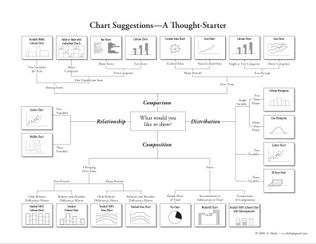
\includegraphics{media/choosing_a_good_chart.jpg}
\caption{}
\end{figure}

\emph{However}, guides which attempt to be comprehensive and show you a
full range of plot types are perhaps not as useful as those which
reflect our knowledge of which plots are the most effective forms of
communication.

For example, almost all guides to plotting, and especially R textbooks,
will show you how to plot a simple bar graph. But bar graphs have
numerous disadvantages over other plots which can show the same
information.

Specifically, they:

\begin{itemize}
\item
  are low in information density (and so inefficient in use of space)
\item
  make comparisons between multiple data series very difficult (for
  example in \protect\hyperlink{understanding-interactions}{interaction
  plots}), and
\item
  perhaps most importantly, even when they include error bars, readers
  consistently misinterpret the quantitative information in bar graphs
  (specifically, when bar graphs are used to display estimates which
  contain error, readers assume points above the bar are less likely
  than points within the bar, even though this is typically not the
  case).
\end{itemize}

You should be guided in choosing plots not by mechanical rules based on
the number or type of variables you want to display. Instead, you should
be guided by the evidence from basic studies of human perception, and
applied data on how different types of infromation displays are really
used by readers.

This guide is restricted to examples likely to be useful and effective
for experiemental and applied psychologists.

\subsubsection*{\texorpdfstring{Thinking like
\texttt{ggplot}}{Thinking like ggplot}}\label{thinking-like-ggplot}
\addcontentsline{toc}{subsubsection}{Thinking like \texttt{ggplot}}

When using \texttt{ggplot} it helps to think of five separate steps to
making a plot (2 are optional, but commonly used):

\begin{enumerate}
\def\labelenumi{\arabic{enumi}.}
\item
  Choose the data you want to plot.
\item
  Map variables to axes or other features of the plot (e.g.~sizes or
  colours).
\item
  (Optionally) use \texttt{ggplot} functions to summarise your data
  before the plot is drawn (e.g.~to calulate means and standard errors
  for point-range plots).
\item
  Add visual display layers.
\item
  (Optionally) Split the plot up across multiple panels using groupings
  in the data.
\end{enumerate}

You can then customise the plot labels and title, and tweak other
presentation parameters, although this often isn't necessary unless
sending a graphic for publication. You can also export graphics in
multiple high quality formats.

The simplest way to demonstrate these steps is with an example, and we
begin with a plot showing the relationship betwen variables:

\subsubsection*{\texorpdfstring{`Relationships'}{Relationships}}\label{relationships}
\addcontentsline{toc}{subsubsection}{`Relationships'}

Problem to be solved: \emph{You want to check/show whether variables are
related in a linear fashion, e.g.~before running linear regression}

\subparagraph{Step 1: Select data to
plot}\label{step-1-select-data-to-plot}
\addcontentsline{toc}{subparagraph}{Step 1: Select data to plot}

Step 1 is to select our data. As is typical in R, \texttt{ggplot} works
best with long-format data. In the examples below we will use the
\texttt{mtcars} dataset for convenience, so our first line of code is to
use the \texttt{dplyr} pipe symbol (operator) to send the
\texttt{mtcars} dataset to the next line of code:

\begin{Shaded}
\begin{Highlighting}[]
\NormalTok{mtcars }\OperatorTok\StringTok{ }
\StringTok{  }\NormalTok{...}
\end{Highlighting}
\end{Shaded}

\subparagraph{Step 2: Map variables to axes, colours, and other
features}\label{step-2-map-variables-to-axes-colours-and-other-features}
\addcontentsline{toc}{subparagraph}{Step 2: Map variables to axes,
colours, and other features}

Step 2 is to map the variables we want to axes or other features of the
plot (e.g.~the colours of points, or the linetypes used in line plots).

The specify these mappings we use the \texttt{aes()} function, which is
slightly cryptic, but short for `aesthetics mapping'. Depending on the
plot type you will specify different aesthetics, and they can also have
different effects depending on the plot type, but you will commonly
specify:

\begin{itemize}
\tightlist
\item
  \texttt{x} the variable to use as the x axis
\item
  \texttt{y} the variable to use as the y axis
\item
  \texttt{colour}: the variable to use to colour points or lines
\end{itemize}

Here we tell \texttt{ggplot} to use \texttt{disp} (engine size) on the x
axis, and \texttt{mpg} on the y axis. We also tell it to colour the
points differently depending on the value of \texttt{hp} (engine
horsepower).

At this point \texttt{ggplot} will create and label the axes and plot
area, but doesn't yet display any of our data. For this we need to add
visual display layers (in the next step).

\begin{Shaded}
\begin{Highlighting}[]
\NormalTok{mtcars }\OperatorTok\StringTok{ }
\StringTok{  }\KeywordTok{ggplot}\NormalTok{(}\KeywordTok{aes}\NormalTok{(}\DataTypeTok{x =}\NormalTok{ disp, }\DataTypeTok{y =}\NormalTok{ mpg, }\DataTypeTok{colour=}\NormalTok{hp))}
\end{Highlighting}
\end{Shaded}

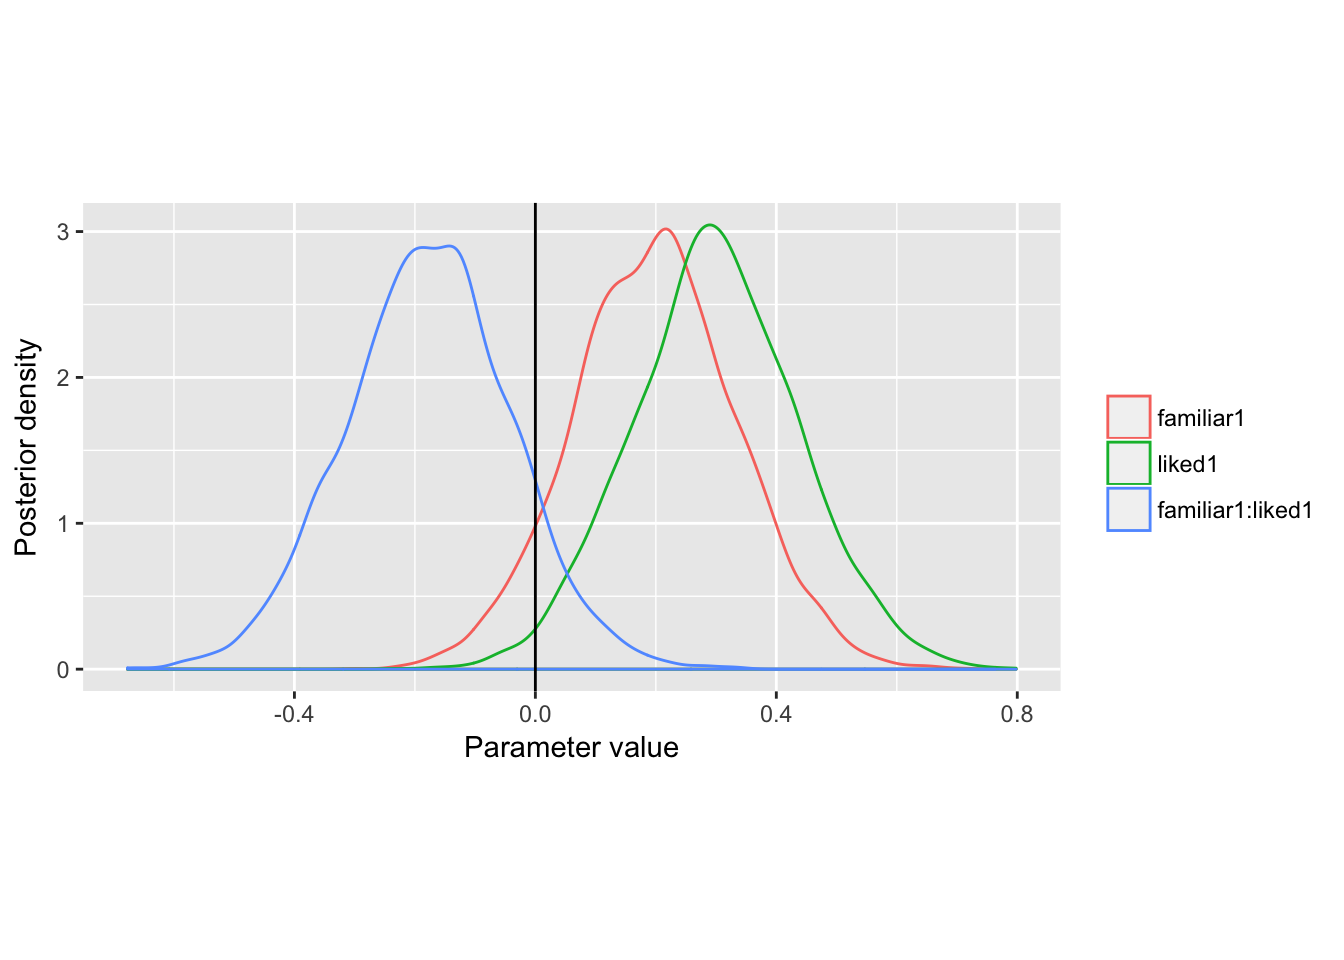
\includegraphics{graphics_files/figure-latex/unnamed-chunk-5-1.pdf}

Other aesthetics

There are many other aesthetics which can be specified. Some of the most
useful are:

\begin{itemize}
\tightlist
\item
  \texttt{ymin} and \texttt{ymax}: for upper and lower bounds, e.g.~on
  error bars
\item
  \texttt{group}:which tells ggplot to group observations by some
  variable and, for example, plot a different line per-group)
\item
  \texttt{fill}: like \texttt{colour} but for areas/shapes
\item
  \texttt{alpha} and \texttt{size}: control the size and opacity of
  visual features (useful for de-emphasising some features of a plot to
  make others stand out)
\end{itemize}

See the ggplot documentation for more details:
\url{http://ggplot2.tidyverse.org/reference/\#section-aesthetics}

\subparagraph{Step 3}\label{step-3}
\addcontentsline{toc}{subparagraph}{Step 3}

We skip step 3 for this example (asking ggplot to automatically make
summaries of our data before plotting), but will cover it below - see
the \texttt{stat\_summary()} function.

\subparagraph{Step 4: Display data}\label{step-4-display-data}
\addcontentsline{toc}{subparagraph}{Step 4: Display data}

To display data, we have to add a visual layer to the plot. For example,
let's say we want to make a scatter plot, and so draw points for each
row of data:

\begin{Shaded}
\begin{Highlighting}[]
\NormalTok{mtcars }\OperatorTok\StringTok{ }
\StringTok{  }\KeywordTok{ggplot}\NormalTok{(}\KeywordTok{aes}\NormalTok{(}\DataTypeTok{x =}\NormalTok{ disp, }\DataTypeTok{y =}\NormalTok{ mpg, }\DataTypeTok{colour=}\NormalTok{hp)) }\OperatorTok{+}
\StringTok{  }\KeywordTok{geom_point}\NormalTok{()}
\end{Highlighting}
\end{Shaded}

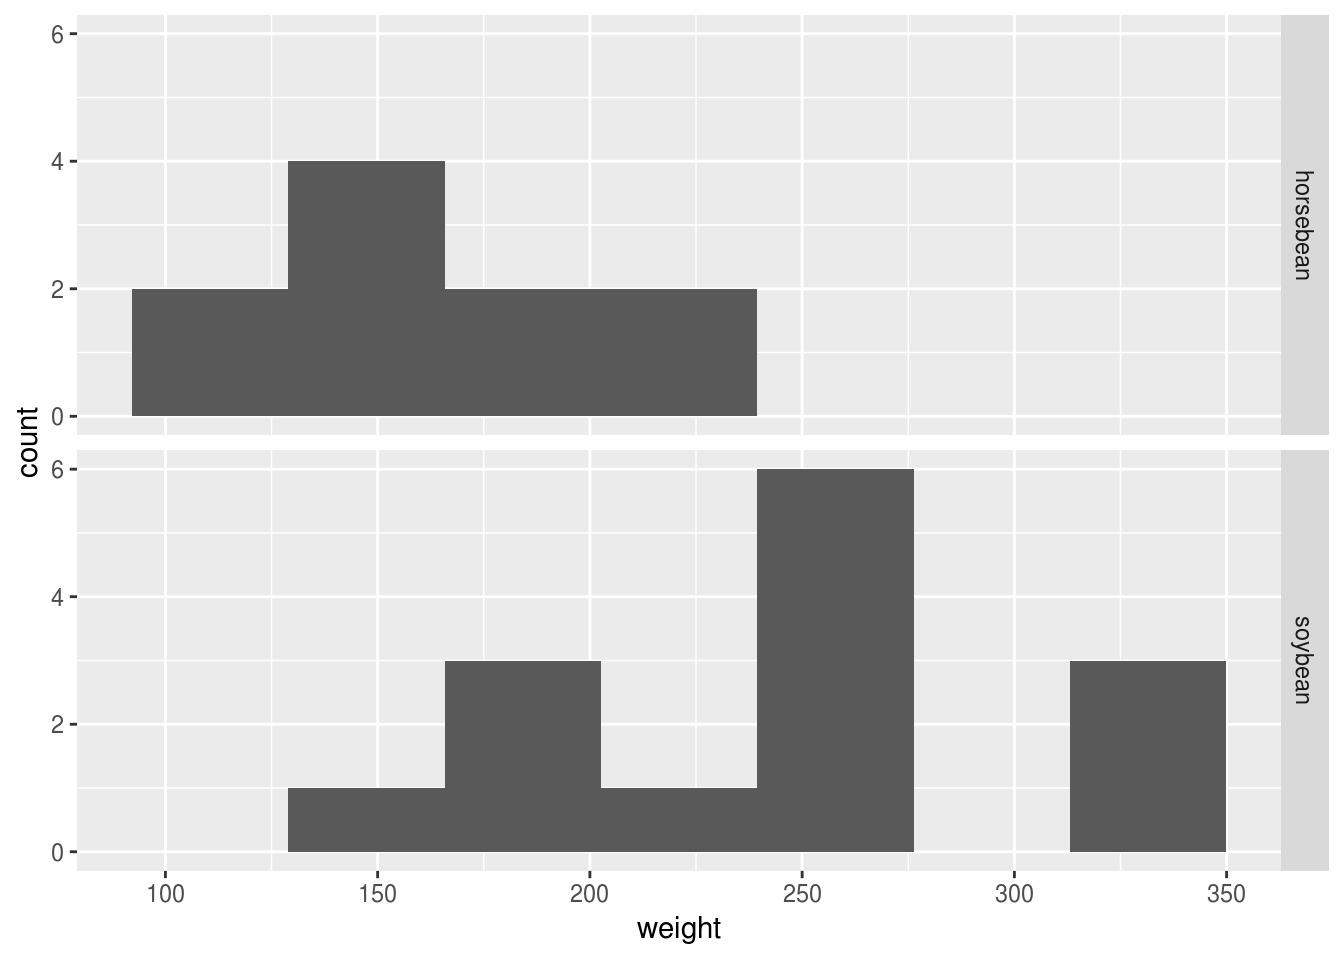
\includegraphics{graphics_files/figure-latex/unnamed-chunk-6-1.pdf}

And we have a pretty slick graph: \texttt{ggplot} has now added points
for each pair of \texttt{disp} and \texttt{mpg} values, and coloured
them according to the value of \texttt{hp} (see choosing colours below
XXX).

{Use the \texttt{airquality} dataset and create your own scatterplot and
try to colour the points using the \texttt{Month} variable. Should
\texttt{Month} be used as a factor or a numeric variable when colouring
the points?}

What's even neater about \texttt{ggplot} though is how easy it is to
\emph{layer} different visualisations of the same data. These visual
layers are called \texttt{geom}'s and the functions which add them are
all prefixed with \texttt{geom\_}, so \texttt{geom\_point()} for scatter
plots, or \texttt{geom\_line()} for line plots, or
\texttt{geom\_smooth()} for a smoothed line plot. We can add this to the
scatter plot like so:

\begin{Shaded}
\begin{Highlighting}[]
\NormalTok{mtcars }\OperatorTok\StringTok{ }
\StringTok{  }\KeywordTok{ggplot}\NormalTok{(}\KeywordTok{aes}\NormalTok{(}\DataTypeTok{x =}\NormalTok{ disp, }\DataTypeTok{y =}\NormalTok{ mpg, }\DataTypeTok{colour=}\NormalTok{hp)) }\OperatorTok{+}
\StringTok{  }\KeywordTok{geom_point}\NormalTok{(}\DataTypeTok{size=}\DecValTok{2}\NormalTok{) }\OperatorTok{+}\StringTok{ }
\StringTok{  }\KeywordTok{geom_smooth}\NormalTok{(}\DataTypeTok{se=}\NormalTok{F, }\DataTypeTok{colour=}\StringTok{"grey"}\NormalTok{) }
\end{Highlighting}
\end{Shaded}

\includegraphics{graphics_files/figure-latex/unnamed-chunk-8-1.pdf}

In the example above, I have also customised the smoothed line, making
it grey to avoid over-intrusion into our perception of the points. Often
less is more when plotting graphs: not everything can be emphasised at
once, and \emph{it's important to make decisions about what should be
given visual priority}.

\subparagraph{\texorpdfstring{Step 5: `Splitting up' or repeating the
plot.}{Step 5: Splitting up or repeating the plot.}}\label{step-5-splitting-up-or-repeating-the-plot.}
\addcontentsline{toc}{subparagraph}{Step 5: `Splitting up' or repeating
the plot.}

Very often, you will have drawn plot and think things like \emph{I
wonder what that would look like if I drew it for men and women
separately?}. In \texttt{ggplot} this is called facetting, and is easy
to achieve, provided your data are in a long format.

Using the same \texttt{mtcars} example, let's say we wanted separate
panels for American vs.~Foreign cars (information held in the
\texttt{am} variable). We simply add the \texttt{facet\_wrap()}, and
specify the \texttt{"am"} variable:

\begin{Shaded}
\begin{Highlighting}[]
\NormalTok{mtcars }\OperatorTok\StringTok{ }
\StringTok{  }\KeywordTok{ggplot}\NormalTok{(}\KeywordTok{aes}\NormalTok{(}\DataTypeTok{x =}\NormalTok{ disp, }\DataTypeTok{y =}\NormalTok{ mpg, }\DataTypeTok{colour=}\NormalTok{hp)) }\OperatorTok{+}
\StringTok{  }\KeywordTok{geom_point}\NormalTok{(}\DataTypeTok{size=}\DecValTok{2}\NormalTok{) }\OperatorTok{+}\StringTok{ }
\StringTok{  }\KeywordTok{geom_smooth}\NormalTok{(}\DataTypeTok{se=}\NormalTok{F, }\DataTypeTok{colour=}\StringTok{"grey"}\NormalTok{) }\OperatorTok{+}
\StringTok{  }\KeywordTok{facet_wrap}\NormalTok{(}\StringTok{"am"}\NormalTok{)}
\end{Highlighting}
\end{Shaded}

\includegraphics{graphics_files/figure-latex/unnamed-chunk-9-1.pdf}

One trick is to make sure factors are labelled nicely, because these
labels appear on the final plot. Here the \texttt{mutate()} call
\href{real-data.html\#factors-and-numerics}{relabels the factor} which
makes the plot easier to read:

\begin{Shaded}
\begin{Highlighting}[]
\NormalTok{mtcars }\OperatorTok\StringTok{ }
\StringTok{  }\KeywordTok{mutate}\NormalTok{(}\DataTypeTok{american =} \KeywordTok{factor}\NormalTok{(am, }\DataTypeTok{labels=}\KeywordTok{c}\NormalTok{(}\StringTok{"American"}\NormalTok{, }\StringTok{"Foreign"}\NormalTok{))) }\OperatorTok\StringTok{ }
\StringTok{  }\KeywordTok{ggplot}\NormalTok{(}\KeywordTok{aes}\NormalTok{(}\DataTypeTok{x =}\NormalTok{ disp, }\DataTypeTok{y =}\NormalTok{ mpg, }\DataTypeTok{colour=}\NormalTok{hp)) }\OperatorTok{+}
\StringTok{  }\KeywordTok{geom_point}\NormalTok{(}\DataTypeTok{size=}\DecValTok{2}\NormalTok{) }\OperatorTok{+}\StringTok{ }
\StringTok{  }\KeywordTok{geom_smooth}\NormalTok{(}\DataTypeTok{se=}\NormalTok{F, }\DataTypeTok{colour=}\StringTok{"grey"}\NormalTok{) }\OperatorTok{+}
\StringTok{  }\KeywordTok{facet_wrap}\NormalTok{(}\StringTok{"american"}\NormalTok{)}
\end{Highlighting}
\end{Shaded}

\includegraphics{graphics_files/figure-latex/unnamed-chunk-10-1.pdf}

\href{http://ggplot2.tidyverse.org/reference/\#section-facetting}{See
the ggplot documentation on facetting for more details}.

\subsubsection*{\texorpdfstring{`Distributions'}{Distributions}}\label{distributions}
\addcontentsline{toc}{subsubsection}{`Distributions'}

\begin{Shaded}
\begin{Highlighting}[]
\NormalTok{lme4}\OperatorTok{::}\NormalTok{sleepstudy }\OperatorTok\StringTok{ }
\StringTok{  }\KeywordTok{ggplot}\NormalTok{(}\KeywordTok{aes}\NormalTok{(Reaction)) }\OperatorTok{+}\StringTok{ }\KeywordTok{geom_density}\NormalTok{()}
\end{Highlighting}
\end{Shaded}

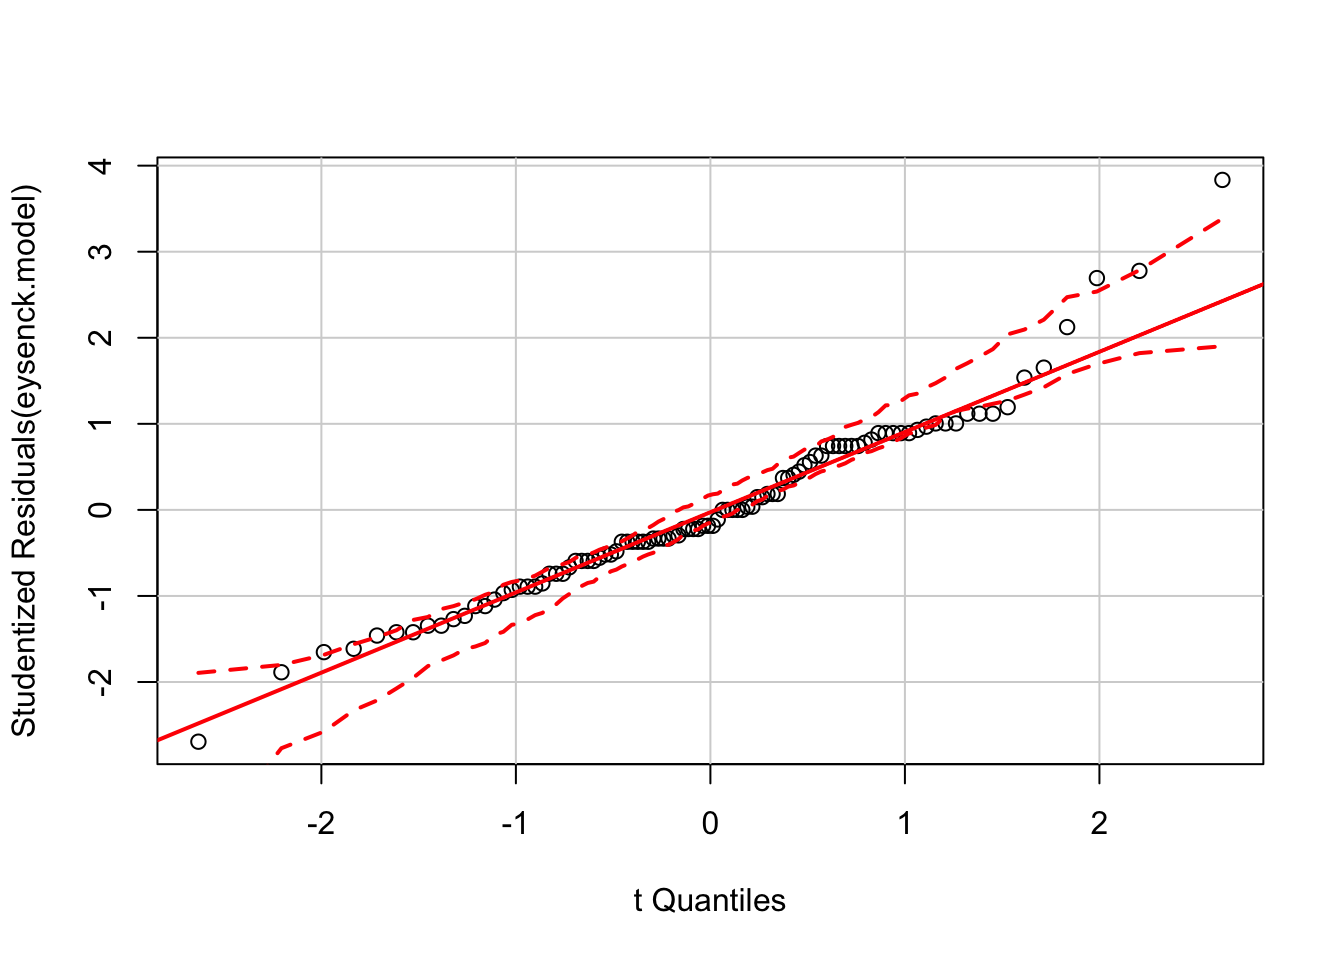
\includegraphics{graphics_files/figure-latex/unnamed-chunk-11-1.pdf}

Imagine we wanted to compare distributions for individuals. Simply
overlaying the lines is confusing:

\begin{Shaded}
\begin{Highlighting}[]
\NormalTok{lme4}\OperatorTok{::}\NormalTok{sleepstudy }\OperatorTok\StringTok{ }
\StringTok{  }\KeywordTok{ggplot}\NormalTok{(}\KeywordTok{aes}\NormalTok{(Reaction, }\DataTypeTok{group=}\NormalTok{Subject)) }\OperatorTok{+}\StringTok{ }\KeywordTok{geom_density}\NormalTok{()}
\end{Highlighting}
\end{Shaded}

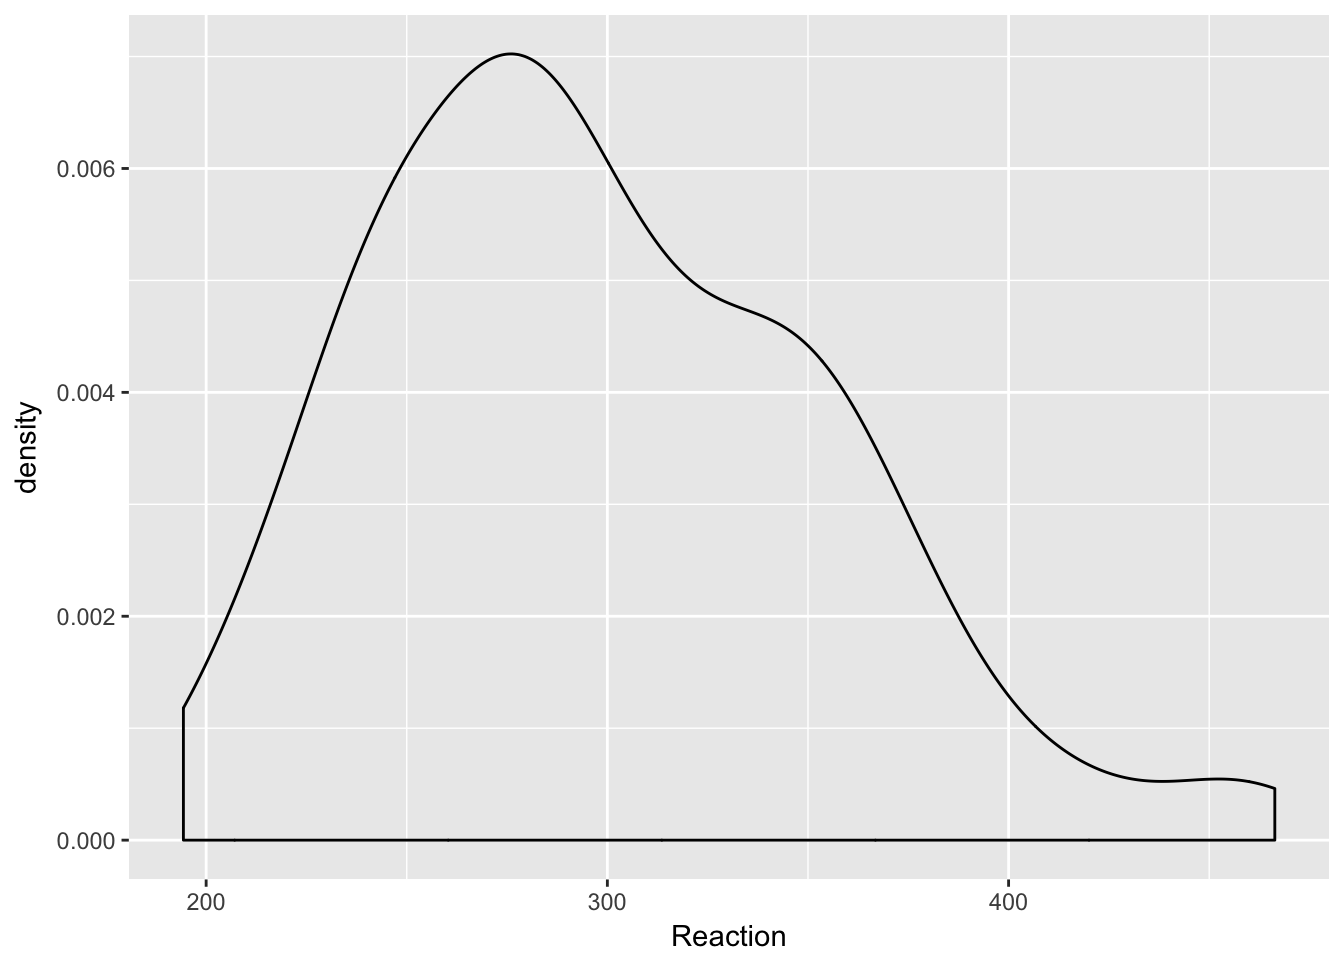
\includegraphics{graphics_files/figure-latex/unnamed-chunk-12-1.pdf}

Facetting produces a nicer result:

\begin{Shaded}
\begin{Highlighting}[]
\NormalTok{lme4}\OperatorTok{::}\NormalTok{sleepstudy }\OperatorTok\StringTok{ }
\StringTok{  }\KeywordTok{ggplot}\NormalTok{(}\KeywordTok{aes}\NormalTok{(Reaction)) }\OperatorTok{+}\StringTok{ }\KeywordTok{geom_density}\NormalTok{() }\OperatorTok{+}\StringTok{ }\KeywordTok{facet_wrap}\NormalTok{(}\StringTok{"Subject"}\NormalTok{)}
\end{Highlighting}
\end{Shaded}

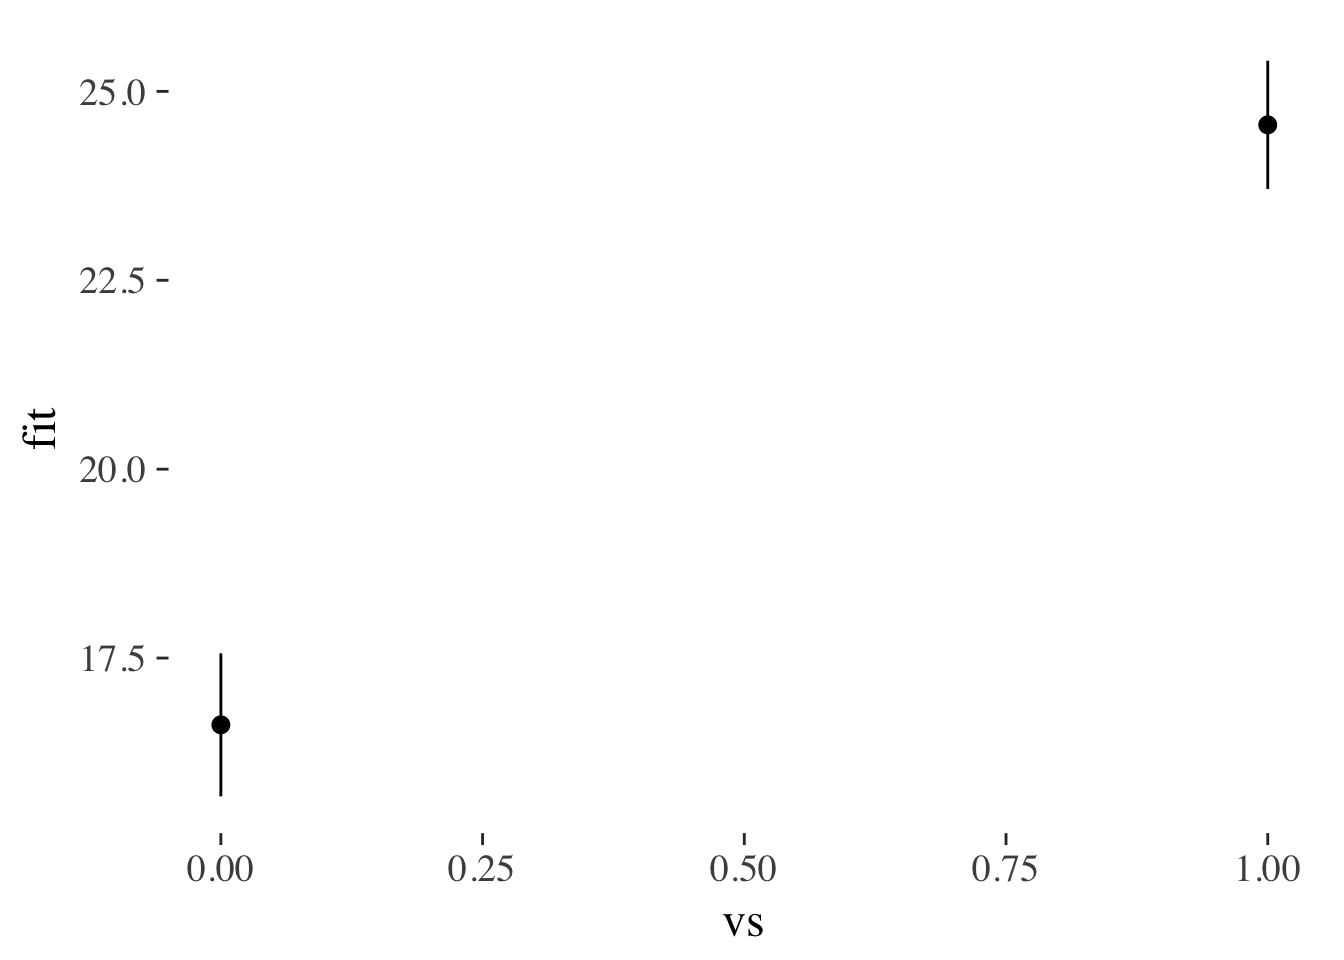
\includegraphics{graphics_files/figure-latex/unnamed-chunk-13-1.pdf}

But we could present the same information more compactly, and with
better facility to compare between subjects, if we use a bottleplot:

\begin{Shaded}
\begin{Highlighting}[]
\NormalTok{lme4}\OperatorTok{::}\NormalTok{sleepstudy }\OperatorTok\StringTok{ }
\StringTok{  }\KeywordTok{ggplot}\NormalTok{(}\KeywordTok{aes}\NormalTok{(Subject, Reaction)) }\OperatorTok{+}\StringTok{ }
\StringTok{  }\KeywordTok{geom_violin}\NormalTok{() }
\end{Highlighting}
\end{Shaded}

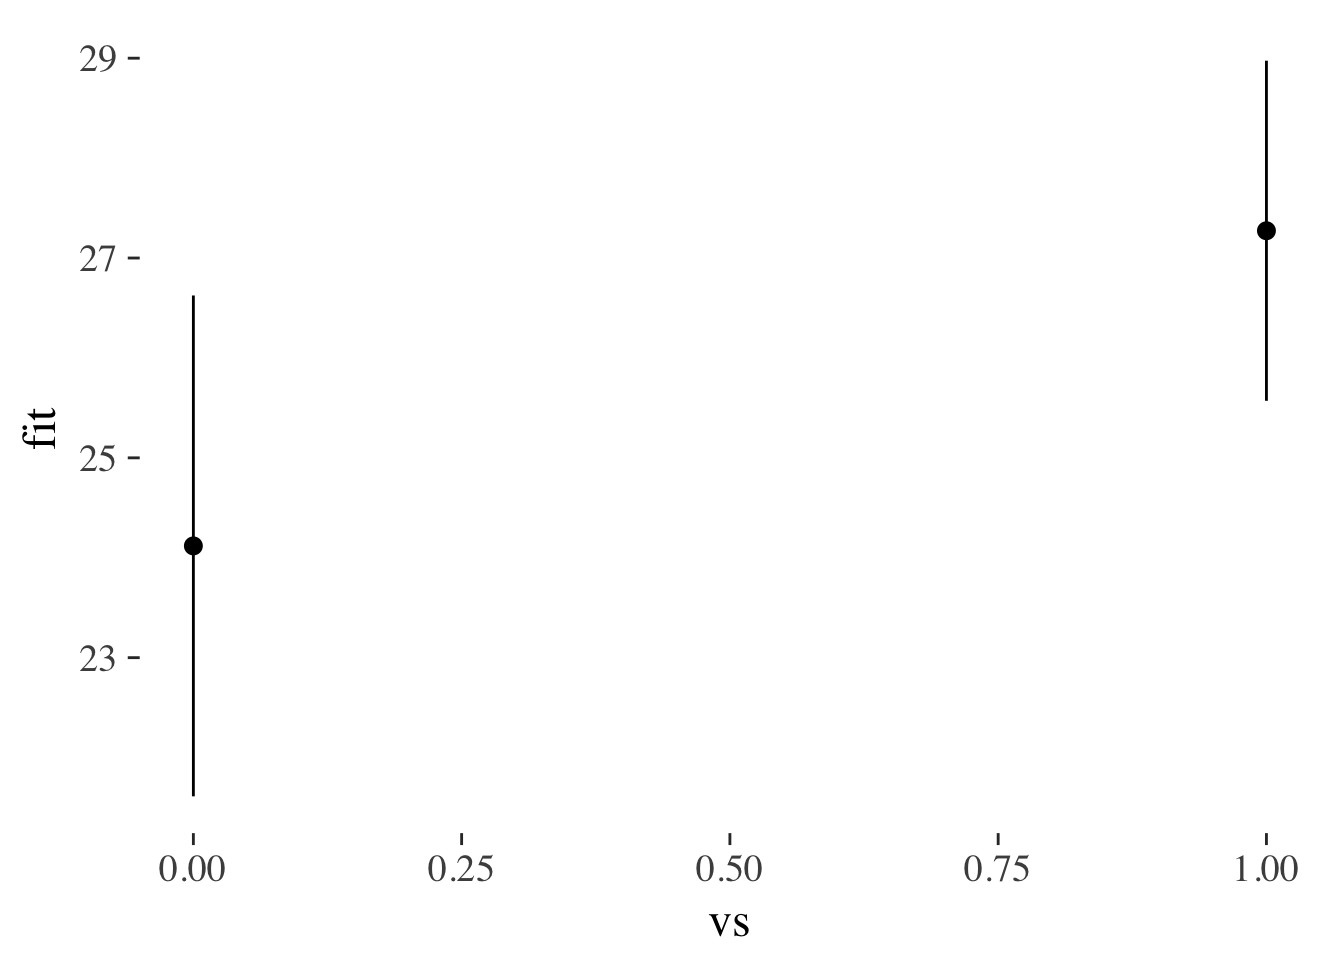
\includegraphics{graphics_files/figure-latex/unnamed-chunk-14-1.pdf}

We might want to plot our Subjects in order of their mean RT:

\begin{Shaded}
\begin{Highlighting}[]
\NormalTok{mean.ranked.sleep <-}\StringTok{ }\NormalTok{lme4}\OperatorTok{::}\NormalTok{sleepstudy }\OperatorTok\StringTok{ }
\StringTok{  }\KeywordTok{group_by}\NormalTok{(Subject) }\OperatorTok\StringTok{ }
\StringTok{  }\CommentTok{# calculate mean RT}
\StringTok{  }\KeywordTok{mutate}\NormalTok{(}\DataTypeTok{RTm =} \KeywordTok{mean}\NormalTok{(Reaction)) }\OperatorTok\StringTok{ }
\StringTok{  }\CommentTok{# sort by mean RT}
\StringTok{  }\KeywordTok{arrange}\NormalTok{(RTm, Days) }\OperatorTok\StringTok{ }
\StringTok{  }\KeywordTok{ungroup}\NormalTok{() }\OperatorTok\StringTok{ }
\StringTok{  }\CommentTok{# create a rank score but conert to factor right away }
\StringTok{  }\KeywordTok{mutate}\NormalTok{(}\DataTypeTok{SubjectRank =} \KeywordTok{factor}\NormalTok{(}\KeywordTok{dense_rank}\NormalTok{(RTm)))}

\NormalTok{mean.ranked.sleep }\OperatorTok\StringTok{ }
\StringTok{  }\KeywordTok{ggplot}\NormalTok{(}\KeywordTok{aes}\NormalTok{(SubjectRank, Reaction)) }\OperatorTok{+}\StringTok{ }
\StringTok{  }\KeywordTok{geom_violin}\NormalTok{() }\OperatorTok{+}\StringTok{ }
\StringTok{  }\KeywordTok{theme}\NormalTok{(}\DataTypeTok{aspect.ratio =}\NormalTok{ .}\DecValTok{33}\NormalTok{)  }\CommentTok{# change the aspect ratio to make long and wide}
\end{Highlighting}
\end{Shaded}

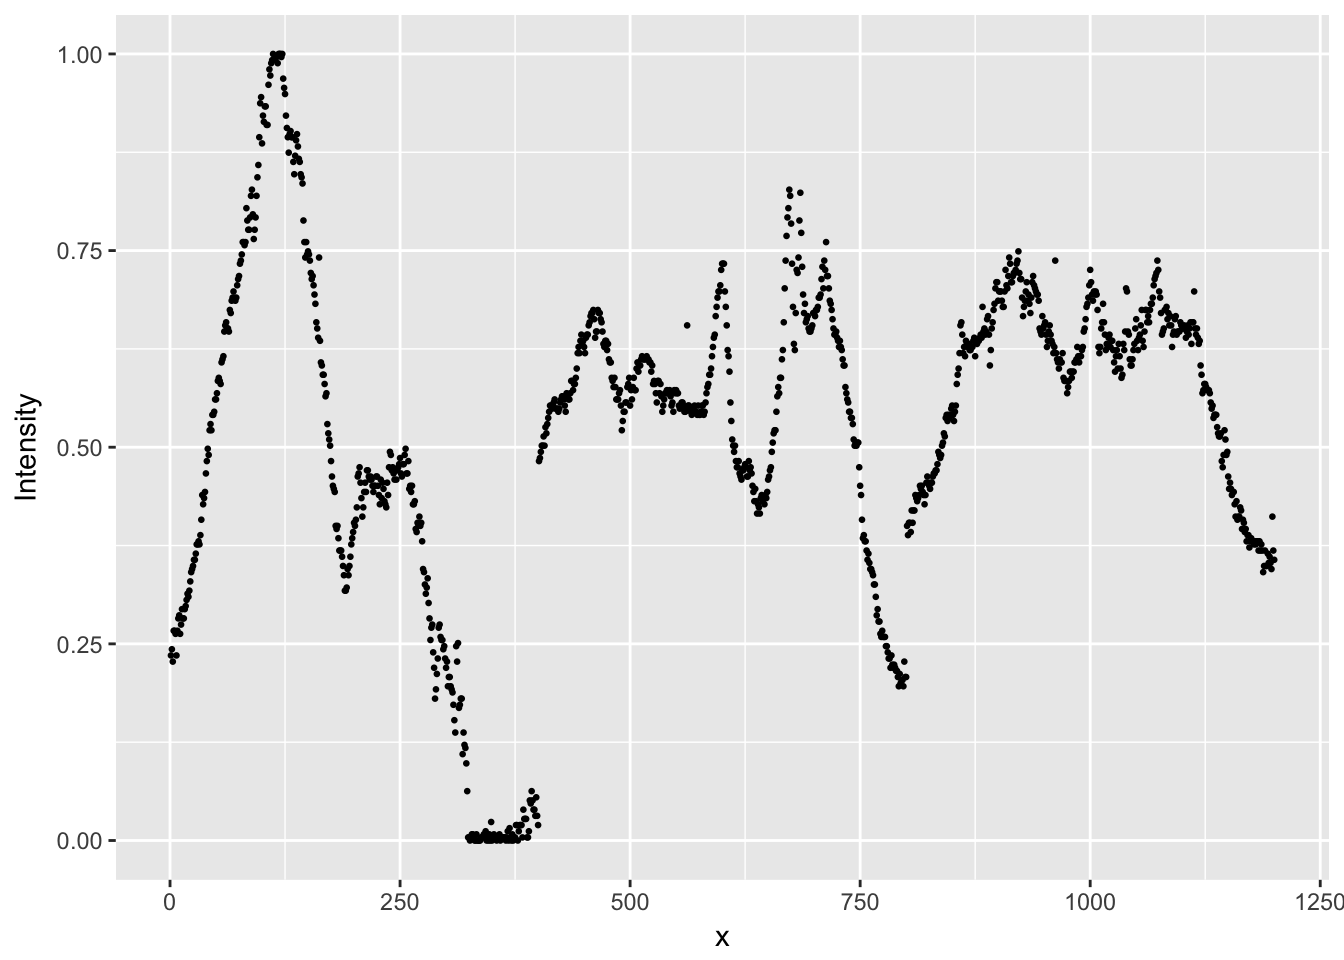
\includegraphics{graphics_files/figure-latex/unnamed-chunk-15-1.pdf}

Or we might want to compare individuals against the combined
distribution:

\begin{Shaded}
\begin{Highlighting}[]
\CommentTok{# duplicate all the data, assigning one-replication to a single subject, "All"}
\NormalTok{sleep.repeat <-}\StringTok{ }\KeywordTok{bind_rows}\NormalTok{(lme4}\OperatorTok{::}\NormalTok{sleepstudy,}
\NormalTok{                          lme4}\OperatorTok{::}\NormalTok{sleepstudy }\OperatorTok\StringTok{ }\KeywordTok{mutate}\NormalTok{(}\DataTypeTok{Subject=}\StringTok{"All"}\NormalTok{))}
\NormalTok{## Warning in bind_rows_(x, .id): binding factor and character vector,}
\NormalTok{## coercing into character vector}
\NormalTok{## Warning in bind_rows_(x, .id): binding character and factor vector,}
\NormalTok{## coercing into character vector}

\NormalTok{sleep.repeat }\OperatorTok\StringTok{ }
\StringTok{  }\KeywordTok{mutate}\NormalTok{(}\DataTypeTok{all =}\NormalTok{ Subject}\OperatorTok{==}\StringTok{"All"}\NormalTok{) }\OperatorTok\StringTok{ }
\StringTok{  }\KeywordTok{ggplot}\NormalTok{(}\KeywordTok{aes}\NormalTok{(Subject, Reaction, }\DataTypeTok{color=}\NormalTok{all)) }\OperatorTok{+}\StringTok{ }
\StringTok{  }\KeywordTok{geom_violin}\NormalTok{() }\OperatorTok{+}
\StringTok{  }\KeywordTok{guides}\NormalTok{(}\DataTypeTok{colour=}\OtherTok{FALSE}\NormalTok{) }\OperatorTok{+}\StringTok{ }\CommentTok{# turn off he legend because we don't really need it}
\StringTok{  }\KeywordTok{theme}\NormalTok{(}\DataTypeTok{aspect.ratio =}\NormalTok{ .}\DecValTok{25}\NormalTok{)  }\CommentTok{# change the aspect ratio to make long and wide}
\end{Highlighting}
\end{Shaded}

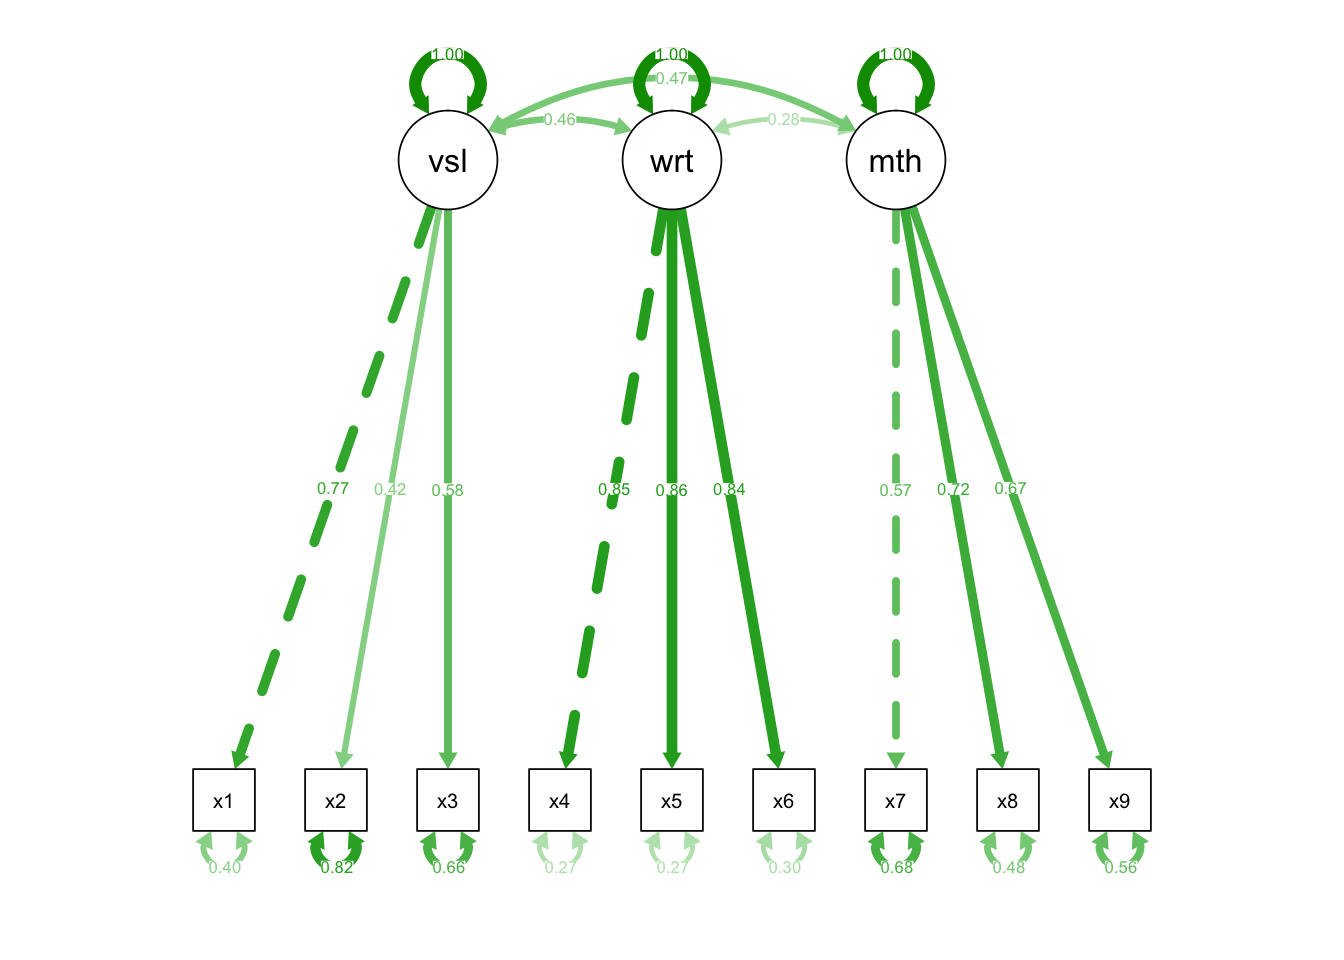
\includegraphics{graphics_files/figure-latex/unnamed-chunk-16-1.pdf}

Boxplots can also work well to show distributions, and have the
advantage of showing the median explicitly:

\begin{Shaded}
\begin{Highlighting}[]
\NormalTok{mean.ranked.sleep }\OperatorTok\StringTok{ }
\StringTok{  }\KeywordTok{ggplot}\NormalTok{(}\KeywordTok{aes}\NormalTok{(SubjectRank, Reaction)) }\OperatorTok{+}\StringTok{ }
\StringTok{  }\KeywordTok{geom_boxplot}\NormalTok{() }
\end{Highlighting}
\end{Shaded}

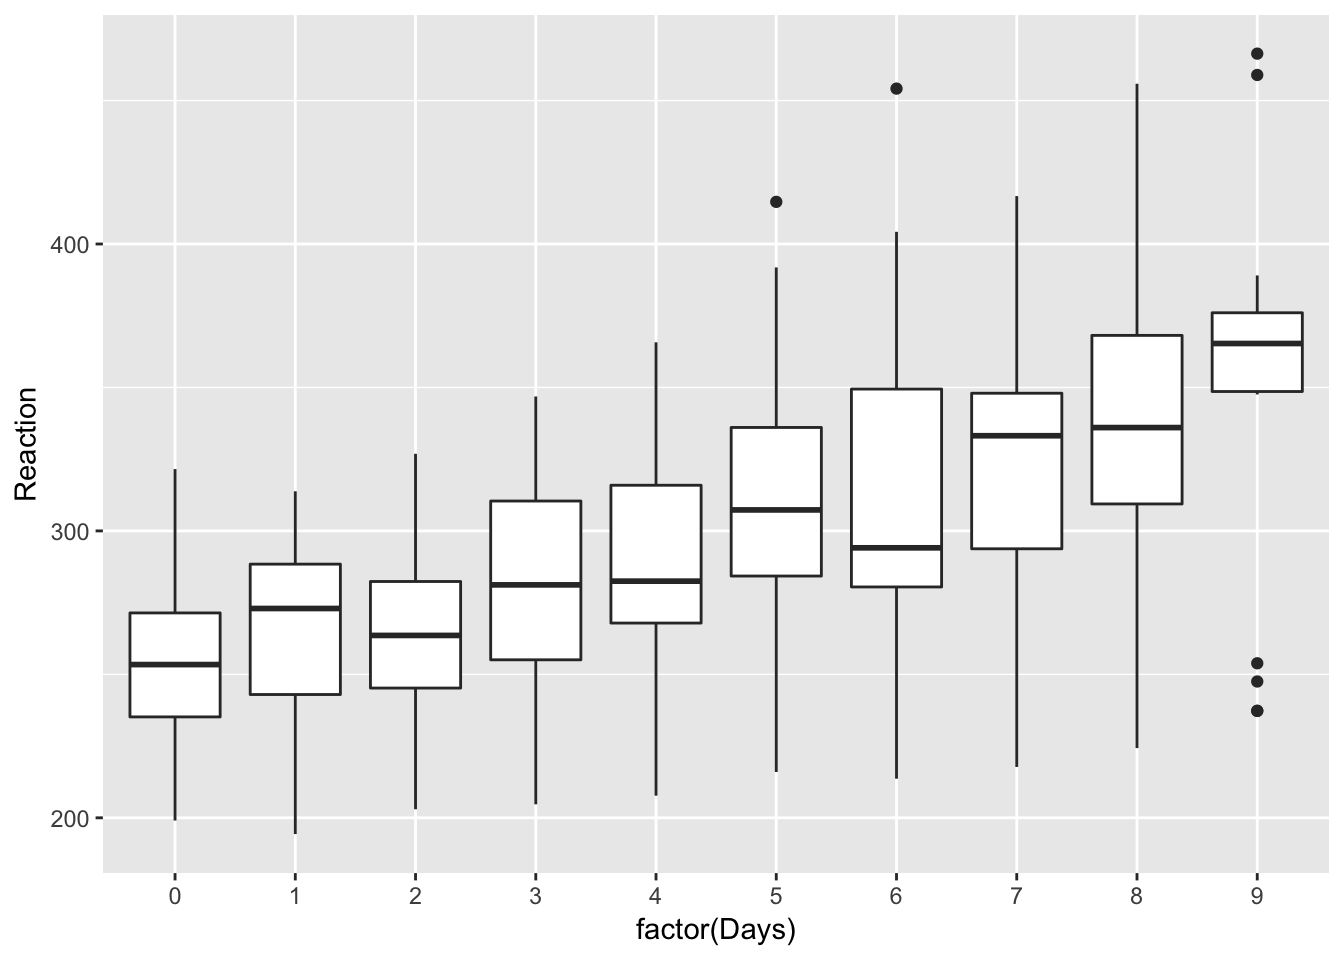
\includegraphics{graphics_files/figure-latex/unnamed-chunk-17-1.pdf}

If we plot the same data by-day, we can clearly see the effect of sleep
deprivation, and the increase in variability between subjects as sime
goes on: the lack of sleeps seems to be affecting some subjects more
than others

\begin{Shaded}
\begin{Highlighting}[]
\NormalTok{lme4}\OperatorTok{::}\NormalTok{sleepstudy }\OperatorTok\StringTok{ }
\StringTok{  }\KeywordTok{ggplot}\NormalTok{(}\KeywordTok{aes}\NormalTok{(}\KeywordTok{factor}\NormalTok{(Days), Reaction)) }\OperatorTok{+}\StringTok{ }
\StringTok{  }\KeywordTok{geom_boxplot}\NormalTok{() }
\end{Highlighting}
\end{Shaded}

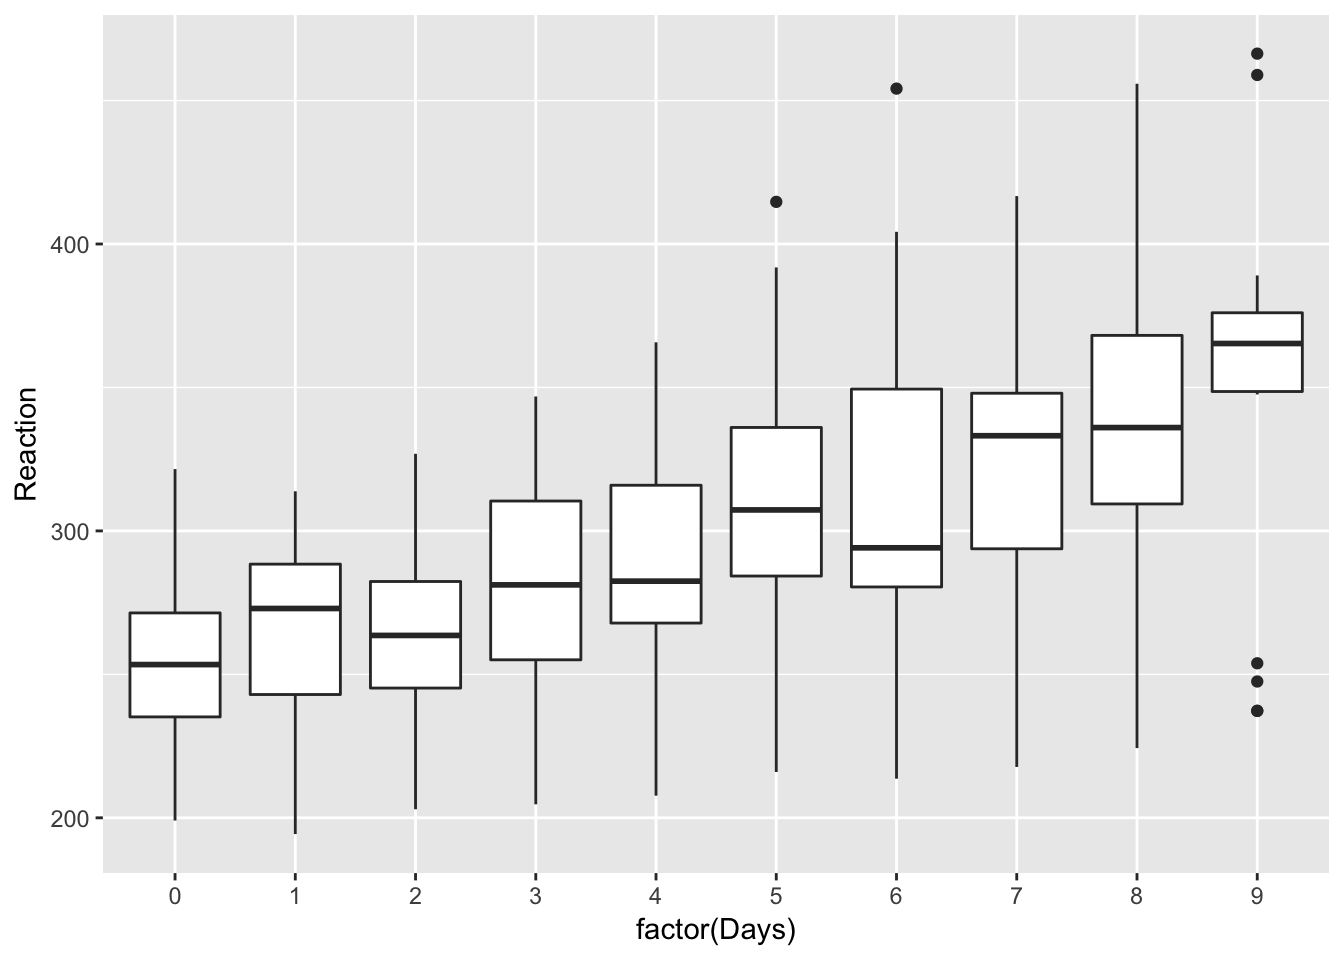
\includegraphics{graphics_files/figure-latex/unnamed-chunk-18-1.pdf}

\subsubsection*{\texorpdfstring{`Comparisons'}{Comparisons}}\label{comparisons}
\addcontentsline{toc}{subsubsection}{`Comparisons'}

Imagine we have rainfall and temperature data for various regions,
across months:

\begin{Shaded}
\begin{Highlighting}[]
\NormalTok{DAAG}\OperatorTok{::}\NormalTok{bomregions }\OperatorTok\StringTok{ }
\StringTok{  }\NormalTok{psych}\OperatorTok{::}\KeywordTok{describe}\NormalTok{(}\DataTypeTok{fast=}\NormalTok{T) }\OperatorTok\StringTok{ }
\StringTok{  }\NormalTok{pander}
\end{Highlighting}
\end{Shaded}

\begin{longtable}[]{@{}ccccccccc@{}}
\toprule
\begin{minipage}[b]{0.14\columnwidth}\centering\strut
~\strut
\end{minipage} & \begin{minipage}[b]{0.06\columnwidth}\centering\strut
vars\strut
\end{minipage} & \begin{minipage}[b]{0.05\columnwidth}\centering\strut
n\strut
\end{minipage} & \begin{minipage}[b]{0.11\columnwidth}\centering\strut
mean\strut
\end{minipage} & \begin{minipage}[b]{0.08\columnwidth}\centering\strut
sd\strut
\end{minipage} & \begin{minipage}[b]{0.08\columnwidth}\centering\strut
min\strut
\end{minipage} & \begin{minipage}[b]{0.07\columnwidth}\centering\strut
max\strut
\end{minipage} & \begin{minipage}[b]{0.07\columnwidth}\centering\strut
range\strut
\end{minipage} & \begin{minipage}[b]{0.08\columnwidth}\centering\strut
se\strut
\end{minipage}\tabularnewline
\midrule
\endhead
\begin{minipage}[t]{0.14\columnwidth}\centering\strut
\textbf{Year}\strut
\end{minipage} & \begin{minipage}[t]{0.06\columnwidth}\centering\strut
1\strut
\end{minipage} & \begin{minipage}[t]{0.05\columnwidth}\centering\strut
109\strut
\end{minipage} & \begin{minipage}[t]{0.11\columnwidth}\centering\strut
1954\strut
\end{minipage} & \begin{minipage}[t]{0.08\columnwidth}\centering\strut
31.61\strut
\end{minipage} & \begin{minipage}[t]{0.08\columnwidth}\centering\strut
1900\strut
\end{minipage} & \begin{minipage}[t]{0.07\columnwidth}\centering\strut
2008\strut
\end{minipage} & \begin{minipage}[t]{0.07\columnwidth}\centering\strut
108\strut
\end{minipage} & \begin{minipage}[t]{0.08\columnwidth}\centering\strut
3.028\strut
\end{minipage}\tabularnewline
\begin{minipage}[t]{0.14\columnwidth}\centering\strut
\textbf{eastAVt}\strut
\end{minipage} & \begin{minipage}[t]{0.06\columnwidth}\centering\strut
2\strut
\end{minipage} & \begin{minipage}[t]{0.05\columnwidth}\centering\strut
99\strut
\end{minipage} & \begin{minipage}[t]{0.11\columnwidth}\centering\strut
20.43\strut
\end{minipage} & \begin{minipage}[t]{0.08\columnwidth}\centering\strut
0.4585\strut
\end{minipage} & \begin{minipage}[t]{0.08\columnwidth}\centering\strut
19.35\strut
\end{minipage} & \begin{minipage}[t]{0.07\columnwidth}\centering\strut
21.61\strut
\end{minipage} & \begin{minipage}[t]{0.07\columnwidth}\centering\strut
2.255\strut
\end{minipage} & \begin{minipage}[t]{0.08\columnwidth}\centering\strut
0.04608\strut
\end{minipage}\tabularnewline
\begin{minipage}[t]{0.14\columnwidth}\centering\strut
\textbf{seAVt}\strut
\end{minipage} & \begin{minipage}[t]{0.06\columnwidth}\centering\strut
3\strut
\end{minipage} & \begin{minipage}[t]{0.05\columnwidth}\centering\strut
99\strut
\end{minipage} & \begin{minipage}[t]{0.11\columnwidth}\centering\strut
14.59\strut
\end{minipage} & \begin{minipage}[t]{0.08\columnwidth}\centering\strut
0.4547\strut
\end{minipage} & \begin{minipage}[t]{0.08\columnwidth}\centering\strut
13.62\strut
\end{minipage} & \begin{minipage}[t]{0.07\columnwidth}\centering\strut
15.94\strut
\end{minipage} & \begin{minipage}[t]{0.07\columnwidth}\centering\strut
2.32\strut
\end{minipage} & \begin{minipage}[t]{0.08\columnwidth}\centering\strut
0.0457\strut
\end{minipage}\tabularnewline
\begin{minipage}[t]{0.14\columnwidth}\centering\strut
\textbf{southAVt}\strut
\end{minipage} & \begin{minipage}[t]{0.06\columnwidth}\centering\strut
4\strut
\end{minipage} & \begin{minipage}[t]{0.05\columnwidth}\centering\strut
99\strut
\end{minipage} & \begin{minipage}[t]{0.11\columnwidth}\centering\strut
18.48\strut
\end{minipage} & \begin{minipage}[t]{0.08\columnwidth}\centering\strut
0.4584\strut
\end{minipage} & \begin{minipage}[t]{0.08\columnwidth}\centering\strut
17.43\strut
\end{minipage} & \begin{minipage}[t]{0.07\columnwidth}\centering\strut
19.53\strut
\end{minipage} & \begin{minipage}[t]{0.07\columnwidth}\centering\strut
2.1\strut
\end{minipage} & \begin{minipage}[t]{0.08\columnwidth}\centering\strut
0.04607\strut
\end{minipage}\tabularnewline
\begin{minipage}[t]{0.14\columnwidth}\centering\strut
\textbf{swAVt}\strut
\end{minipage} & \begin{minipage}[t]{0.06\columnwidth}\centering\strut
5\strut
\end{minipage} & \begin{minipage}[t]{0.05\columnwidth}\centering\strut
99\strut
\end{minipage} & \begin{minipage}[t]{0.11\columnwidth}\centering\strut
16.18\strut
\end{minipage} & \begin{minipage}[t]{0.08\columnwidth}\centering\strut
0.4734\strut
\end{minipage} & \begin{minipage}[t]{0.08\columnwidth}\centering\strut
15.08\strut
\end{minipage} & \begin{minipage}[t]{0.07\columnwidth}\centering\strut
17.05\strut
\end{minipage} & \begin{minipage}[t]{0.07\columnwidth}\centering\strut
1.97\strut
\end{minipage} & \begin{minipage}[t]{0.08\columnwidth}\centering\strut
0.04758\strut
\end{minipage}\tabularnewline
\begin{minipage}[t]{0.14\columnwidth}\centering\strut
\textbf{westAVt}\strut
\end{minipage} & \begin{minipage}[t]{0.06\columnwidth}\centering\strut
6\strut
\end{minipage} & \begin{minipage}[t]{0.05\columnwidth}\centering\strut
99\strut
\end{minipage} & \begin{minipage}[t]{0.11\columnwidth}\centering\strut
22.33\strut
\end{minipage} & \begin{minipage}[t]{0.08\columnwidth}\centering\strut
0.4548\strut
\end{minipage} & \begin{minipage}[t]{0.08\columnwidth}\centering\strut
21.22\strut
\end{minipage} & \begin{minipage}[t]{0.07\columnwidth}\centering\strut
23.39\strut
\end{minipage} & \begin{minipage}[t]{0.07\columnwidth}\centering\strut
2.165\strut
\end{minipage} & \begin{minipage}[t]{0.08\columnwidth}\centering\strut
0.04571\strut
\end{minipage}\tabularnewline
\begin{minipage}[t]{0.14\columnwidth}\centering\strut
\textbf{northAVt}\strut
\end{minipage} & \begin{minipage}[t]{0.06\columnwidth}\centering\strut
7\strut
\end{minipage} & \begin{minipage}[t]{0.05\columnwidth}\centering\strut
99\strut
\end{minipage} & \begin{minipage}[t]{0.11\columnwidth}\centering\strut
24.6\strut
\end{minipage} & \begin{minipage}[t]{0.08\columnwidth}\centering\strut
0.5042\strut
\end{minipage} & \begin{minipage}[t]{0.08\columnwidth}\centering\strut
23.57\strut
\end{minipage} & \begin{minipage}[t]{0.07\columnwidth}\centering\strut
25.94\strut
\end{minipage} & \begin{minipage}[t]{0.07\columnwidth}\centering\strut
2.365\strut
\end{minipage} & \begin{minipage}[t]{0.08\columnwidth}\centering\strut
0.05067\strut
\end{minipage}\tabularnewline
\begin{minipage}[t]{0.14\columnwidth}\centering\strut
\textbf{mdbAVt}\strut
\end{minipage} & \begin{minipage}[t]{0.06\columnwidth}\centering\strut
8\strut
\end{minipage} & \begin{minipage}[t]{0.05\columnwidth}\centering\strut
99\strut
\end{minipage} & \begin{minipage}[t]{0.11\columnwidth}\centering\strut
17.59\strut
\end{minipage} & \begin{minipage}[t]{0.08\columnwidth}\centering\strut
0.4958\strut
\end{minipage} & \begin{minipage}[t]{0.08\columnwidth}\centering\strut
16.36\strut
\end{minipage} & \begin{minipage}[t]{0.07\columnwidth}\centering\strut
18.79\strut
\end{minipage} & \begin{minipage}[t]{0.07\columnwidth}\centering\strut
2.425\strut
\end{minipage} & \begin{minipage}[t]{0.08\columnwidth}\centering\strut
0.04983\strut
\end{minipage}\tabularnewline
\begin{minipage}[t]{0.14\columnwidth}\centering\strut
\textbf{auAVt}\strut
\end{minipage} & \begin{minipage}[t]{0.06\columnwidth}\centering\strut
9\strut
\end{minipage} & \begin{minipage}[t]{0.05\columnwidth}\centering\strut
99\strut
\end{minipage} & \begin{minipage}[t]{0.11\columnwidth}\centering\strut
21.71\strut
\end{minipage} & \begin{minipage}[t]{0.08\columnwidth}\centering\strut
0.4429\strut
\end{minipage} & \begin{minipage}[t]{0.08\columnwidth}\centering\strut
20.67\strut
\end{minipage} & \begin{minipage}[t]{0.07\columnwidth}\centering\strut
22.87\strut
\end{minipage} & \begin{minipage}[t]{0.07\columnwidth}\centering\strut
2.195\strut
\end{minipage} & \begin{minipage}[t]{0.08\columnwidth}\centering\strut
0.04452\strut
\end{minipage}\tabularnewline
\begin{minipage}[t]{0.14\columnwidth}\centering\strut
\textbf{eastRain}\strut
\end{minipage} & \begin{minipage}[t]{0.06\columnwidth}\centering\strut
10\strut
\end{minipage} & \begin{minipage}[t]{0.05\columnwidth}\centering\strut
109\strut
\end{minipage} & \begin{minipage}[t]{0.11\columnwidth}\centering\strut
601.6\strut
\end{minipage} & \begin{minipage}[t]{0.08\columnwidth}\centering\strut
123.8\strut
\end{minipage} & \begin{minipage}[t]{0.08\columnwidth}\centering\strut
315.3\strut
\end{minipage} & \begin{minipage}[t]{0.07\columnwidth}\centering\strut
1030\strut
\end{minipage} & \begin{minipage}[t]{0.07\columnwidth}\centering\strut
715\strut
\end{minipage} & \begin{minipage}[t]{0.08\columnwidth}\centering\strut
11.85\strut
\end{minipage}\tabularnewline
\begin{minipage}[t]{0.14\columnwidth}\centering\strut
\textbf{seRain}\strut
\end{minipage} & \begin{minipage}[t]{0.06\columnwidth}\centering\strut
11\strut
\end{minipage} & \begin{minipage}[t]{0.05\columnwidth}\centering\strut
109\strut
\end{minipage} & \begin{minipage}[t]{0.11\columnwidth}\centering\strut
598.1\strut
\end{minipage} & \begin{minipage}[t]{0.08\columnwidth}\centering\strut
104.6\strut
\end{minipage} & \begin{minipage}[t]{0.08\columnwidth}\centering\strut
354.9\strut
\end{minipage} & \begin{minipage}[t]{0.07\columnwidth}\centering\strut
900.6\strut
\end{minipage} & \begin{minipage}[t]{0.07\columnwidth}\centering\strut
545.7\strut
\end{minipage} & \begin{minipage}[t]{0.08\columnwidth}\centering\strut
10.02\strut
\end{minipage}\tabularnewline
\begin{minipage}[t]{0.14\columnwidth}\centering\strut
\textbf{southRain}\strut
\end{minipage} & \begin{minipage}[t]{0.06\columnwidth}\centering\strut
12\strut
\end{minipage} & \begin{minipage}[t]{0.05\columnwidth}\centering\strut
109\strut
\end{minipage} & \begin{minipage}[t]{0.11\columnwidth}\centering\strut
381.7\strut
\end{minipage} & \begin{minipage}[t]{0.08\columnwidth}\centering\strut
68.63\strut
\end{minipage} & \begin{minipage}[t]{0.08\columnwidth}\centering\strut
236\strut
\end{minipage} & \begin{minipage}[t]{0.07\columnwidth}\centering\strut
618.2\strut
\end{minipage} & \begin{minipage}[t]{0.07\columnwidth}\centering\strut
382.1\strut
\end{minipage} & \begin{minipage}[t]{0.08\columnwidth}\centering\strut
6.574\strut
\end{minipage}\tabularnewline
\begin{minipage}[t]{0.14\columnwidth}\centering\strut
\textbf{swRain}\strut
\end{minipage} & \begin{minipage}[t]{0.06\columnwidth}\centering\strut
13\strut
\end{minipage} & \begin{minipage}[t]{0.05\columnwidth}\centering\strut
109\strut
\end{minipage} & \begin{minipage}[t]{0.11\columnwidth}\centering\strut
657.8\strut
\end{minipage} & \begin{minipage}[t]{0.08\columnwidth}\centering\strut
103\strut
\end{minipage} & \begin{minipage}[t]{0.08\columnwidth}\centering\strut
420.5\strut
\end{minipage} & \begin{minipage}[t]{0.07\columnwidth}\centering\strut
988.8\strut
\end{minipage} & \begin{minipage}[t]{0.07\columnwidth}\centering\strut
568.4\strut
\end{minipage} & \begin{minipage}[t]{0.08\columnwidth}\centering\strut
9.861\strut
\end{minipage}\tabularnewline
\begin{minipage}[t]{0.14\columnwidth}\centering\strut
\textbf{westRain}\strut
\end{minipage} & \begin{minipage}[t]{0.06\columnwidth}\centering\strut
14\strut
\end{minipage} & \begin{minipage}[t]{0.05\columnwidth}\centering\strut
109\strut
\end{minipage} & \begin{minipage}[t]{0.11\columnwidth}\centering\strut
352.2\strut
\end{minipage} & \begin{minipage}[t]{0.08\columnwidth}\centering\strut
84.55\strut
\end{minipage} & \begin{minipage}[t]{0.08\columnwidth}\centering\strut
173.5\strut
\end{minipage} & \begin{minipage}[t]{0.07\columnwidth}\centering\strut
646.5\strut
\end{minipage} & \begin{minipage}[t]{0.07\columnwidth}\centering\strut
473\strut
\end{minipage} & \begin{minipage}[t]{0.08\columnwidth}\centering\strut
8.098\strut
\end{minipage}\tabularnewline
\begin{minipage}[t]{0.14\columnwidth}\centering\strut
\textbf{northRain}\strut
\end{minipage} & \begin{minipage}[t]{0.06\columnwidth}\centering\strut
15\strut
\end{minipage} & \begin{minipage}[t]{0.05\columnwidth}\centering\strut
109\strut
\end{minipage} & \begin{minipage}[t]{0.11\columnwidth}\centering\strut
520.7\strut
\end{minipage} & \begin{minipage}[t]{0.08\columnwidth}\centering\strut
110.2\strut
\end{minipage} & \begin{minipage}[t]{0.08\columnwidth}\centering\strut
312.8\strut
\end{minipage} & \begin{minipage}[t]{0.07\columnwidth}\centering\strut
946.9\strut
\end{minipage} & \begin{minipage}[t]{0.07\columnwidth}\centering\strut
634\strut
\end{minipage} & \begin{minipage}[t]{0.08\columnwidth}\centering\strut
10.55\strut
\end{minipage}\tabularnewline
\begin{minipage}[t]{0.14\columnwidth}\centering\strut
\textbf{mdbRain}\strut
\end{minipage} & \begin{minipage}[t]{0.06\columnwidth}\centering\strut
16\strut
\end{minipage} & \begin{minipage}[t]{0.05\columnwidth}\centering\strut
109\strut
\end{minipage} & \begin{minipage}[t]{0.11\columnwidth}\centering\strut
476\strut
\end{minipage} & \begin{minipage}[t]{0.08\columnwidth}\centering\strut
110.9\strut
\end{minipage} & \begin{minipage}[t]{0.08\columnwidth}\centering\strut
255.8\strut
\end{minipage} & \begin{minipage}[t]{0.07\columnwidth}\centering\strut
821\strut
\end{minipage} & \begin{minipage}[t]{0.07\columnwidth}\centering\strut
565.2\strut
\end{minipage} & \begin{minipage}[t]{0.08\columnwidth}\centering\strut
10.62\strut
\end{minipage}\tabularnewline
\begin{minipage}[t]{0.14\columnwidth}\centering\strut
\textbf{auRain}\strut
\end{minipage} & \begin{minipage}[t]{0.06\columnwidth}\centering\strut
17\strut
\end{minipage} & \begin{minipage}[t]{0.05\columnwidth}\centering\strut
109\strut
\end{minipage} & \begin{minipage}[t]{0.11\columnwidth}\centering\strut
457.1\strut
\end{minipage} & \begin{minipage}[t]{0.08\columnwidth}\centering\strut
82.55\strut
\end{minipage} & \begin{minipage}[t]{0.08\columnwidth}\centering\strut
317.2\strut
\end{minipage} & \begin{minipage}[t]{0.07\columnwidth}\centering\strut
785.3\strut
\end{minipage} & \begin{minipage}[t]{0.07\columnwidth}\centering\strut
468.1\strut
\end{minipage} & \begin{minipage}[t]{0.08\columnwidth}\centering\strut
7.906\strut
\end{minipage}\tabularnewline
\begin{minipage}[t]{0.14\columnwidth}\centering\strut
\textbf{SOI}\strut
\end{minipage} & \begin{minipage}[t]{0.06\columnwidth}\centering\strut
18\strut
\end{minipage} & \begin{minipage}[t]{0.05\columnwidth}\centering\strut
109\strut
\end{minipage} & \begin{minipage}[t]{0.11\columnwidth}\centering\strut
-0.002676\strut
\end{minipage} & \begin{minipage}[t]{0.08\columnwidth}\centering\strut
6.845\strut
\end{minipage} & \begin{minipage}[t]{0.08\columnwidth}\centering\strut
-20.01\strut
\end{minipage} & \begin{minipage}[t]{0.07\columnwidth}\centering\strut
20.79\strut
\end{minipage} & \begin{minipage}[t]{0.07\columnwidth}\centering\strut
40.8\strut
\end{minipage} & \begin{minipage}[t]{0.08\columnwidth}\centering\strut
0.6556\strut
\end{minipage}\tabularnewline
\begin{minipage}[t]{0.14\columnwidth}\centering\strut
\textbf{co2mlo}\strut
\end{minipage} & \begin{minipage}[t]{0.06\columnwidth}\centering\strut
19\strut
\end{minipage} & \begin{minipage}[t]{0.05\columnwidth}\centering\strut
50\strut
\end{minipage} & \begin{minipage}[t]{0.11\columnwidth}\centering\strut
345.6\strut
\end{minipage} & \begin{minipage}[t]{0.08\columnwidth}\centering\strut
21.01\strut
\end{minipage} & \begin{minipage}[t]{0.08\columnwidth}\centering\strut
316\strut
\end{minipage} & \begin{minipage}[t]{0.07\columnwidth}\centering\strut
385.4\strut
\end{minipage} & \begin{minipage}[t]{0.07\columnwidth}\centering\strut
69.47\strut
\end{minipage} & \begin{minipage}[t]{0.08\columnwidth}\centering\strut
2.972\strut
\end{minipage}\tabularnewline
\begin{minipage}[t]{0.14\columnwidth}\centering\strut
\textbf{co2law}\strut
\end{minipage} & \begin{minipage}[t]{0.06\columnwidth}\centering\strut
20\strut
\end{minipage} & \begin{minipage}[t]{0.05\columnwidth}\centering\strut
79\strut
\end{minipage} & \begin{minipage}[t]{0.11\columnwidth}\centering\strut
310.4\strut
\end{minipage} & \begin{minipage}[t]{0.08\columnwidth}\centering\strut
9.586\strut
\end{minipage} & \begin{minipage}[t]{0.08\columnwidth}\centering\strut
295.8\strut
\end{minipage} & \begin{minipage}[t]{0.07\columnwidth}\centering\strut
333.7\strut
\end{minipage} & \begin{minipage}[t]{0.07\columnwidth}\centering\strut
37.9\strut
\end{minipage} & \begin{minipage}[t]{0.08\columnwidth}\centering\strut
1.078\strut
\end{minipage}\tabularnewline
\begin{minipage}[t]{0.14\columnwidth}\centering\strut
\textbf{CO2}\strut
\end{minipage} & \begin{minipage}[t]{0.06\columnwidth}\centering\strut
21\strut
\end{minipage} & \begin{minipage}[t]{0.05\columnwidth}\centering\strut
109\strut
\end{minipage} & \begin{minipage}[t]{0.11\columnwidth}\centering\strut
324.3\strut
\end{minipage} & \begin{minipage}[t]{0.08\columnwidth}\centering\strut
24.59\strut
\end{minipage} & \begin{minipage}[t]{0.08\columnwidth}\centering\strut
296.3\strut
\end{minipage} & \begin{minipage}[t]{0.07\columnwidth}\centering\strut
385.4\strut
\end{minipage} & \begin{minipage}[t]{0.07\columnwidth}\centering\strut
89.19\strut
\end{minipage} & \begin{minipage}[t]{0.08\columnwidth}\centering\strut
2.355\strut
\end{minipage}\tabularnewline
\begin{minipage}[t]{0.14\columnwidth}\centering\strut
\textbf{sunspot}\strut
\end{minipage} & \begin{minipage}[t]{0.06\columnwidth}\centering\strut
22\strut
\end{minipage} & \begin{minipage}[t]{0.05\columnwidth}\centering\strut
109\strut
\end{minipage} & \begin{minipage}[t]{0.11\columnwidth}\centering\strut
60.08\strut
\end{minipage} & \begin{minipage}[t]{0.08\columnwidth}\centering\strut
47.69\strut
\end{minipage} & \begin{minipage}[t]{0.08\columnwidth}\centering\strut
1.4\strut
\end{minipage} & \begin{minipage}[t]{0.07\columnwidth}\centering\strut
190.2\strut
\end{minipage} & \begin{minipage}[t]{0.07\columnwidth}\centering\strut
188.8\strut
\end{minipage} & \begin{minipage}[t]{0.08\columnwidth}\centering\strut
4.568\strut
\end{minipage}\tabularnewline
\bottomrule
\end{longtable}

\hypertarget{extract-to-split-column-names}{\subparagraph{}\label{extract-to-split-column-names}}
\addcontentsline{toc}{subparagraph}{}

Because these data are in wide format (multiple columns have contain the
same type of data) we need to first convert to long format. This process
has become known as \href{http://tidyr.tidyverse.org}{tidying}.

The code below selects the columns related to rainfall and temperature
and then `melts' the data to long format: one row per observation. We
then \texttt{extract} the region and the type of measurement from the
\texttt{variable} column which is created by using a regular expression:

\begin{Shaded}
\begin{Highlighting}[]
\NormalTok{weather.data.long <-}\StringTok{ }\NormalTok{DAAG}\OperatorTok{::}\NormalTok{bomregions }\OperatorTok\StringTok{ }
\StringTok{  }\KeywordTok{select}\NormalTok{(Year, }\KeywordTok{ends_with}\NormalTok{(}\StringTok{'Rain'}\NormalTok{), }\KeywordTok{ends_with}\NormalTok{(}\StringTok{'AVt'}\NormalTok{)) }\OperatorTok\StringTok{ }
\StringTok{  }\NormalTok{reshape2}\OperatorTok{::}\KeywordTok{melt}\NormalTok{(}\DataTypeTok{id.var=}\StringTok{"Year"}\NormalTok{) }\OperatorTok\StringTok{ }
\StringTok{  }\KeywordTok{extract}\NormalTok{(variable, }
          \DataTypeTok{into=}\KeywordTok{c}\NormalTok{(}\StringTok{"Region"}\NormalTok{, }\StringTok{"variable"}\NormalTok{), }
          \DataTypeTok{regex=}\StringTok{"(east|north|se|south|west|sw|au)(}\CharTok{\textbackslash{}\textbackslash{}}\StringTok{w+)"}\NormalTok{) }\OperatorTok\StringTok{ }
\StringTok{  }\KeywordTok{filter}\NormalTok{(}\OperatorTok{!}\KeywordTok{is.na}\NormalTok{(variable))}

\NormalTok{weather.data.long }\OperatorTok\StringTok{ }\NormalTok{head}
\NormalTok{##   Year Region variable  value}
\NormalTok{## 1 1900   east     Rain 429.98}
\NormalTok{## 2 1901   east     Rain 500.12}
\NormalTok{## 3 1902   east     Rain 315.33}
\NormalTok{## 4 1903   east     Rain 694.09}
\NormalTok{## 5 1904   east     Rain 564.86}
\NormalTok{## 6 1905   east     Rain 443.11}
\end{Highlighting}
\end{Shaded}

\subparagraph{}\label{section-12}

Try stepping through the code above line by line and see what is
produced at each step.

With our data in long form we can use \texttt{ggplot} to plot our data
over time. In the plot below, we use \texttt{filter()} to select only
the rainfall measurements:

\begin{Shaded}
\begin{Highlighting}[]
\NormalTok{rain <-}\StringTok{ }
\StringTok{  }\NormalTok{weather.data.long }\OperatorTok\StringTok{ }
\StringTok{  }\KeywordTok{filter}\NormalTok{(variable}\OperatorTok{==}\StringTok{'Rain'}\NormalTok{)}

\NormalTok{rain }\OperatorTok\StringTok{ }
\StringTok{  }\KeywordTok{ggplot}\NormalTok{(}\KeywordTok{aes}\NormalTok{(Year, value)) }\OperatorTok{+}
\StringTok{  }\KeywordTok{geom_point}\NormalTok{() }\OperatorTok{+}\StringTok{ }
\StringTok{  }\KeywordTok{ylab}\NormalTok{(}\StringTok{'Rainfall (mm)'}\NormalTok{)}
\end{Highlighting}
\end{Shaded}

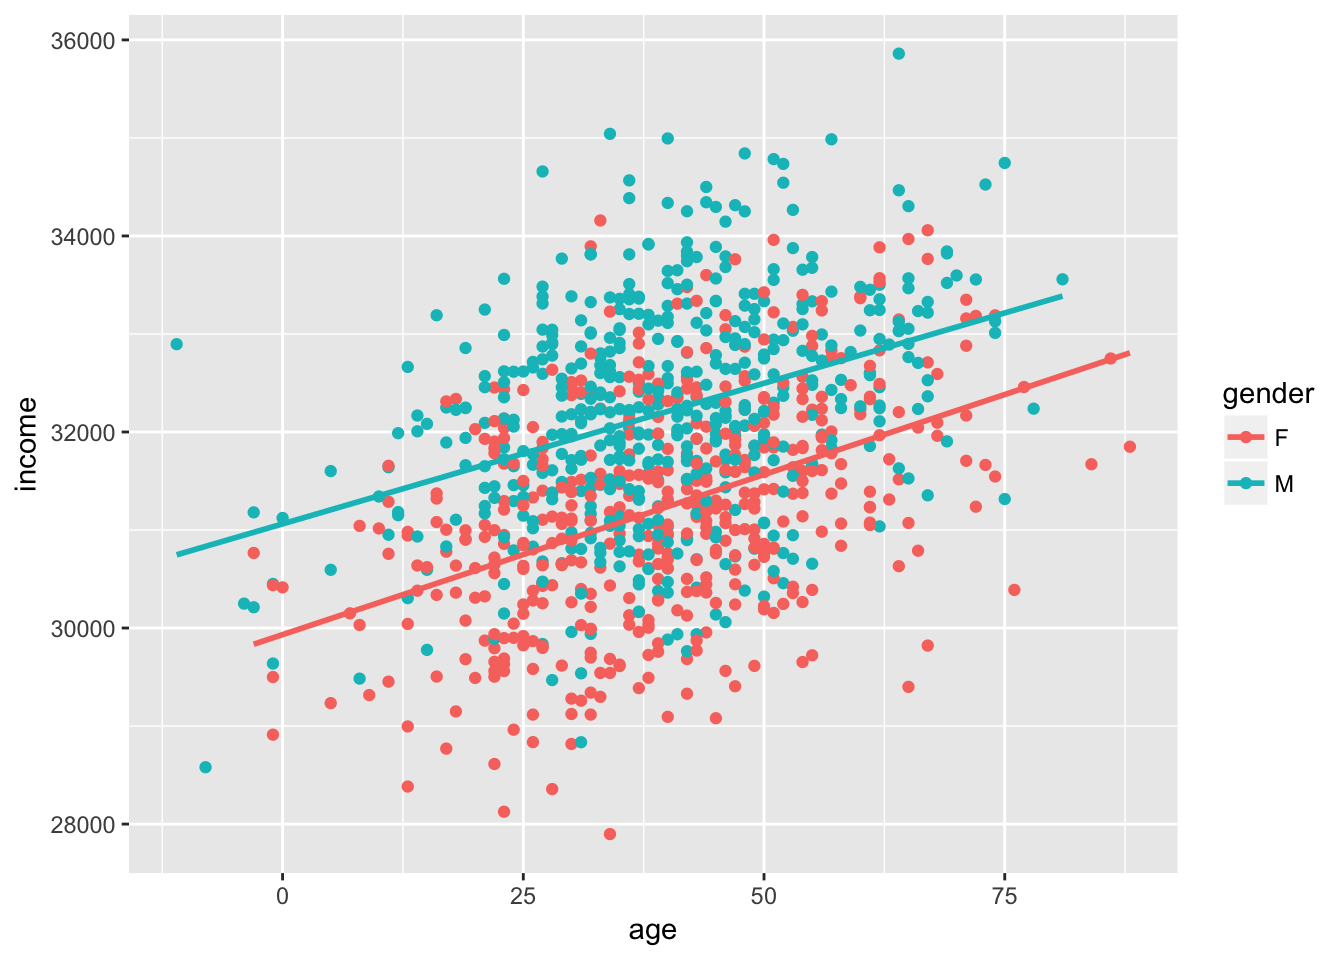
\includegraphics{graphics_files/figure-latex/unnamed-chunk-21-1.pdf}

There are many ways to extract structure from these data, and make
comparisons over time. One is to use colour:

\begin{Shaded}
\begin{Highlighting}[]
\NormalTok{rain }\OperatorTok\StringTok{ }
\StringTok{  }\KeywordTok{ggplot}\NormalTok{(}\KeywordTok{aes}\NormalTok{(Year, value, }\DataTypeTok{color=}\NormalTok{Region)) }\OperatorTok{+}
\StringTok{  }\KeywordTok{geom_point}\NormalTok{() }\OperatorTok{+}
\StringTok{  }\KeywordTok{ylab}\NormalTok{(}\StringTok{'Rainfall (mm)'}\NormalTok{)}
\end{Highlighting}
\end{Shaded}

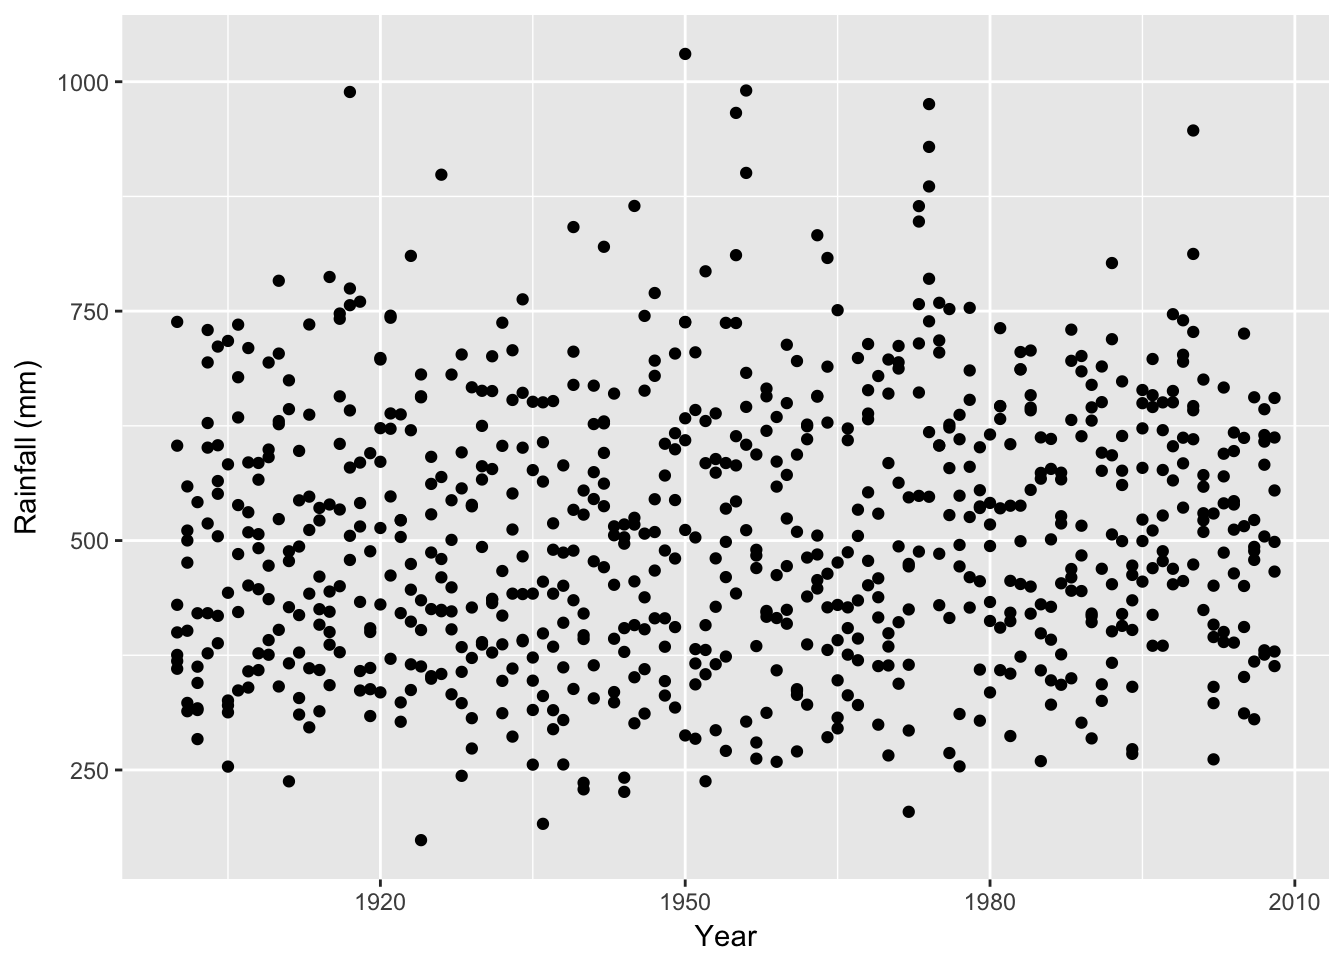
\includegraphics{graphics_files/figure-latex/unnamed-chunk-22-1.pdf}

It's now easy to see the crude differences between the regions (west
appears the driest, sw the wettest), but it's still hard to compare
between regions, or over time.

For this we can use various forms of summaries, for example a smoothed
line plot (the shaded area is the standard error), which clearly shows
the relative changes in rainfall in each region over time:

\begin{Shaded}
\begin{Highlighting}[]
\NormalTok{rain }\OperatorTok\StringTok{ }
\StringTok{  }\KeywordTok{ggplot}\NormalTok{(}\KeywordTok{aes}\NormalTok{(Year, value, }\DataTypeTok{color=}\NormalTok{Region)) }\OperatorTok{+}
\StringTok{  }\KeywordTok{geom_smooth}\NormalTok{() }\OperatorTok{+}
\StringTok{  }\KeywordTok{ylab}\NormalTok{(}\StringTok{'Rainfall (mm)'}\NormalTok{)}
\end{Highlighting}
\end{Shaded}

\includegraphics{graphics_files/figure-latex/unnamed-chunk-23-1.pdf}

It can sometimes be desireable to include points to preserve the
relationship between the summary and the raw data:

\begin{Shaded}
\begin{Highlighting}[]
\NormalTok{rain }\OperatorTok\StringTok{ }
\StringTok{  }\KeywordTok{filter}\NormalTok{(Region }\OperatorTok\StringTok{ }\KeywordTok{c}\NormalTok{(}\StringTok{'west'}\NormalTok{, }\StringTok{'se'}\NormalTok{)) }\OperatorTok\StringTok{ }
\StringTok{  }\KeywordTok{ggplot}\NormalTok{(}\KeywordTok{aes}\NormalTok{(Year, value, }\DataTypeTok{color=}\NormalTok{Region)) }\OperatorTok{+}
\StringTok{  }\KeywordTok{geom_point}\NormalTok{(}\DataTypeTok{alpha=}\NormalTok{.}\DecValTok{5}\NormalTok{, }\DataTypeTok{size=}\NormalTok{.}\DecValTok{5}\NormalTok{) }\OperatorTok{+}
\StringTok{  }\KeywordTok{geom_smooth}\NormalTok{(}\DataTypeTok{se=}\NormalTok{F) }\OperatorTok{+}
\StringTok{  }\KeywordTok{ylab}\NormalTok{(}\StringTok{'Rainfall (mm)'}\NormalTok{)}
\end{Highlighting}
\end{Shaded}

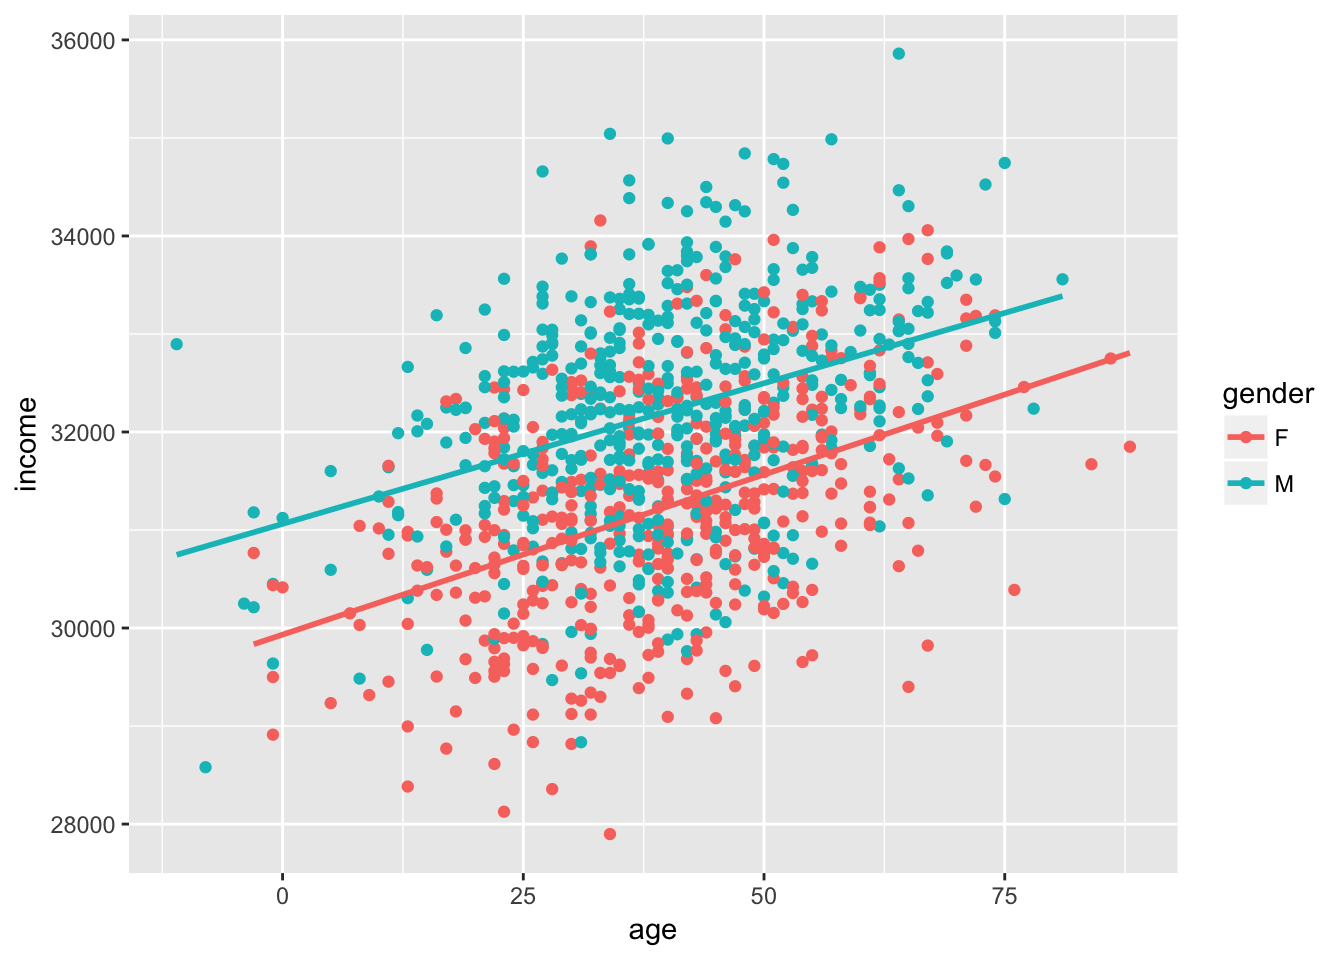
\includegraphics{graphics_files/figure-latex/unnamed-chunk-24-1.pdf}

If we weren't interested in the time series and just wanted to focus on
the most recent year, we might take a different approach. Here a bar
plot is used to compare between regions, with the national average (au)
highlighted in blue:

\begin{Shaded}
\begin{Highlighting}[]
\NormalTok{rain }\OperatorTok\StringTok{ }
\StringTok{  }\KeywordTok{filter}\NormalTok{(Year }\OperatorTok{==}\StringTok{ }\KeywordTok{max}\NormalTok{(Year)) }\OperatorTok\StringTok{ }
\StringTok{  }\KeywordTok{ggplot}\NormalTok{(}\KeywordTok{aes}\NormalTok{(Region, value, }\DataTypeTok{fill=}\NormalTok{Region}\OperatorTok{==}\StringTok{"au"}\NormalTok{)) }\OperatorTok{+}
\StringTok{  }\KeywordTok{stat_summary}\NormalTok{(}\DataTypeTok{geom=}\StringTok{"bar"}\NormalTok{) }\OperatorTok{+}
\StringTok{  }\KeywordTok{ylab}\NormalTok{(}\StringTok{'Rainfall (mm)'}\NormalTok{) }\OperatorTok{+}\StringTok{ }
\StringTok{  }\KeywordTok{guides}\NormalTok{(}\DataTypeTok{fill=}\NormalTok{F)}
\end{Highlighting}
\end{Shaded}

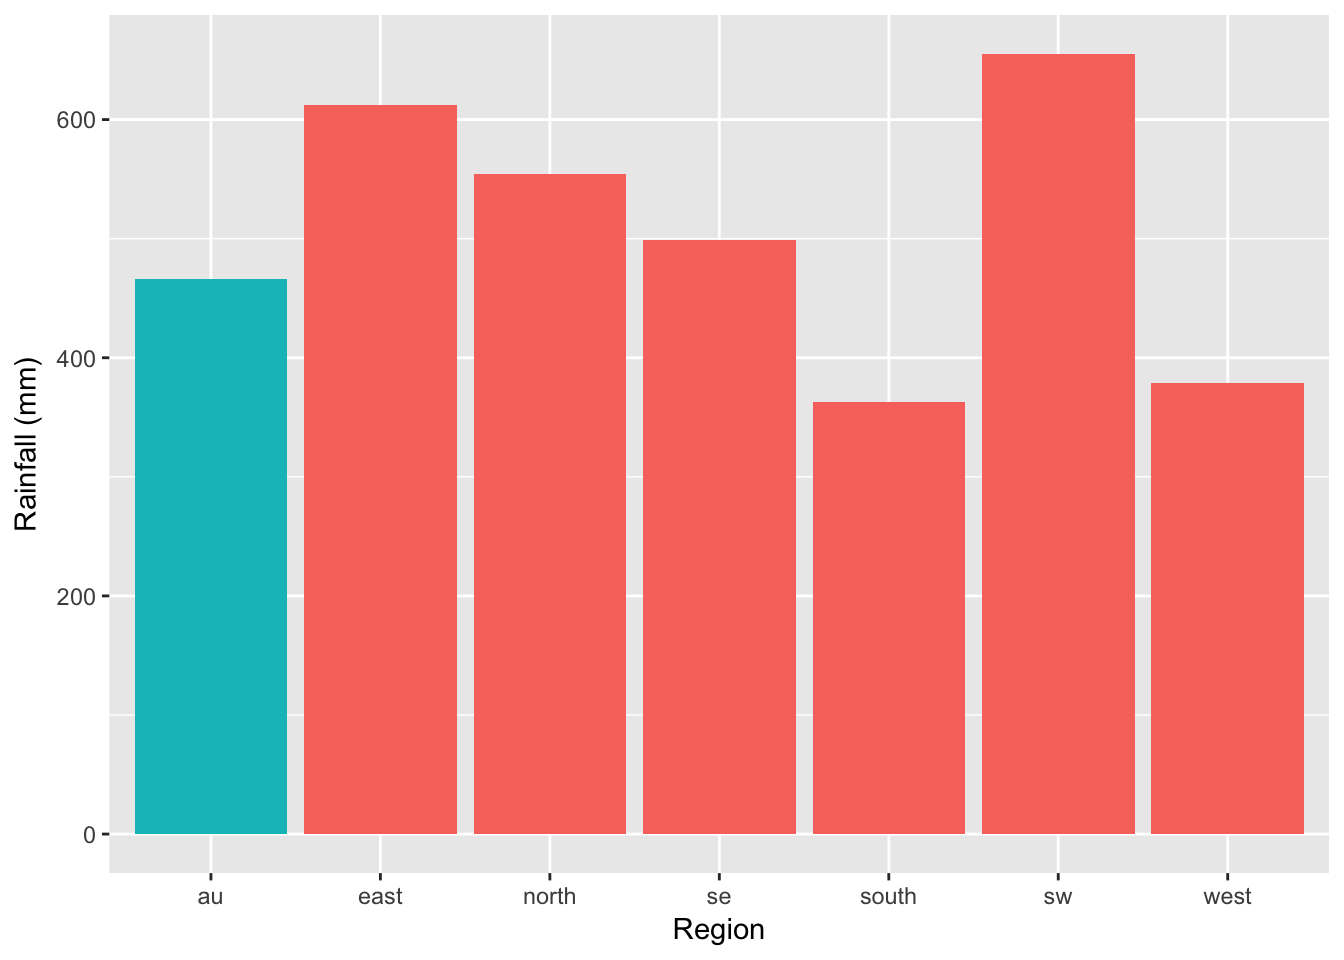
\includegraphics{graphics_files/figure-latex/unnamed-chunk-25-1.pdf}

Finally, we shouldn't forget that this dataset included both rainfall
and temperature data, and we can display these in different ways,
depending on what our research question was.

In this case we can use facetting to display temperature and rainfall
data side by side. Because AVt and Rain are on such different scales we
need to allow the y axis to vary between variables:

\begin{Shaded}
\begin{Highlighting}[]
\NormalTok{weather.data.long }\OperatorTok\StringTok{ }
\StringTok{  }\KeywordTok{ggplot}\NormalTok{(}\KeywordTok{aes}\NormalTok{(Year, value, }\DataTypeTok{color=}\NormalTok{Region)) }\OperatorTok{+}\StringTok{ }
\StringTok{  }\KeywordTok{geom_smooth}\NormalTok{() }\OperatorTok{+}\StringTok{ }
\StringTok{  }\KeywordTok{facet_wrap}\NormalTok{(}\OperatorTok{~}\NormalTok{variable, }\DataTypeTok{scales=}\StringTok{"free"}\NormalTok{)}
\NormalTok{## Warning: Removed 70 rows containing non-finite values (stat_smooth).}
\end{Highlighting}
\end{Shaded}

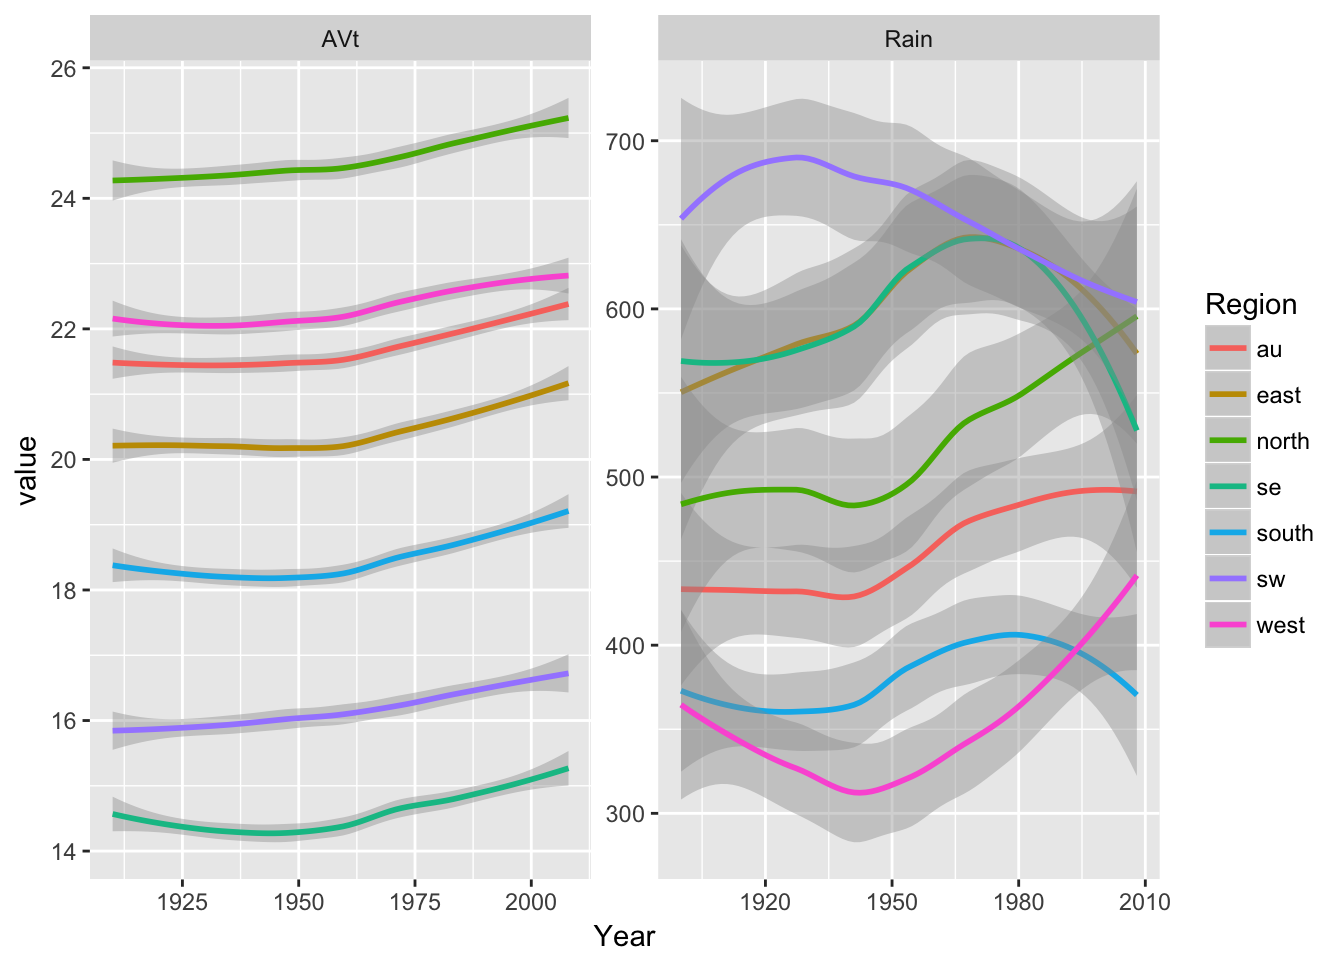
\includegraphics{graphics_files/figure-latex/unnamed-chunk-26-1.pdf}

\subsubsection*{\texorpdfstring{`Composition'}{Composition}}\label{composition}
\addcontentsline{toc}{subsubsection}{`Composition'}

\paragraph{\texorpdfstring{Waffle plots or
`pictograms'}{Waffle plots or pictograms}}\label{waffle-plots-or-pictograms}
\addcontentsline{toc}{paragraph}{Waffle plots or `pictograms'}

Waffle plots are neat way of showing the relative frequency of different
categories.

In applied settings it's well known that when considering the risks or
benefits of interventions clinicans, patients and researchers benefit
from statements made using `natural frequencies'
\citep{gigerenzer2003simple}, and pictographs or `waffle plots' have
been shown to provide patients and their families with a better
understanding of the risks of treatments \citep{tait2010presenting}.

Waffle plots can be implemented in R via the \texttt{waffle::} package:

\begin{Shaded}
\begin{Highlighting}[]
\NormalTok{outcomes <-}\StringTok{ }\KeywordTok{c}\NormalTok{(}\StringTok{"gained weight"}\NormalTok{=}\DecValTok{13}\NormalTok{, }
              \StringTok{"no change"}\NormalTok{=}\DecValTok{27}\NormalTok{, }
              \StringTok{"lost 2kg or more"}\NormalTok{ =}\StringTok{ }\DecValTok{44}\NormalTok{, }
              \StringTok{"lost 5kg or more"}\NormalTok{ =}\StringTok{ }\DecValTok{16}\NormalTok{)}

\NormalTok{waffle}\OperatorTok{::}\KeywordTok{waffle}\NormalTok{(outcomes)}
\end{Highlighting}
\end{Shaded}

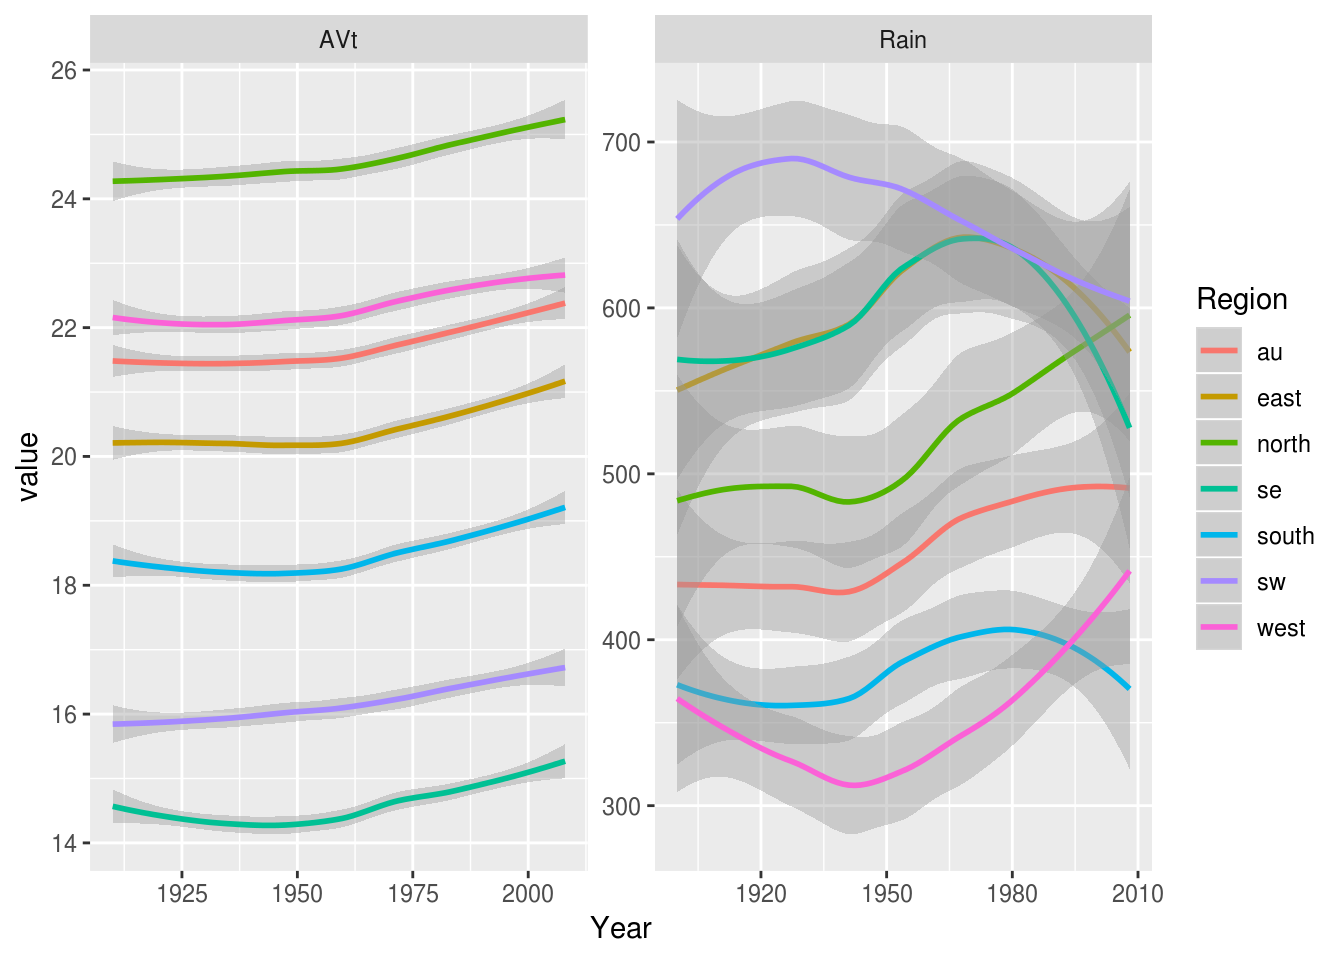
\includegraphics{graphics_files/figure-latex/unnamed-chunk-27-1.pdf}

{Calculating these summary figures is left as an exercise to for the
reader, but see the section on
\protect\hyperlink{split-apply-combine}{summarising data with dplyr}.}

This is one of those occasions where the default ggplot colours could
probably be improved, and we can do this by passing the
\protect\hyperlink{named-colours}{names of the colours} we would like to
use:

\begin{Shaded}
\begin{Highlighting}[]
\NormalTok{weight.loss.colours <-}\StringTok{ }\KeywordTok{c}\NormalTok{(}\StringTok{'firebrick2'}\NormalTok{, }\StringTok{'darkgoldenrod1'}\NormalTok{, }\StringTok{'palegreen3'}\NormalTok{, }\StringTok{'palegreen4'}\NormalTok{)}
\NormalTok{waffle}\OperatorTok{::}\KeywordTok{waffle}\NormalTok{(outcomes, }\DataTypeTok{colors =}\NormalTok{ weight.loss.colours)}
\end{Highlighting}
\end{Shaded}

\includegraphics{graphics_files/figure-latex/unnamed-chunk-28-1.pdf}

Selecting colours by hand isn't always the best way though: the
\protect\hyperlink{color-brewer}{\texttt{colourbrewer} library provides
some nice shortcuts} for using palletes from the excellent
\href{http://colorbrewer2.org}{ColourBrewer website}.

\paragraph{Stacked bars}\label{stacked-bars}
\addcontentsline{toc}{paragraph}{Stacked bars}

The \texttt{reshape2} package includes data on tipping habits in
restaurants for male and female bill-payers, and where the party was fo
various \texttt{size}s:

\begin{Shaded}
\begin{Highlighting}[]
\NormalTok{reshape2}\OperatorTok{::}\NormalTok{tips }\OperatorTok\StringTok{ }
\StringTok{  }\NormalTok{head }\OperatorTok\StringTok{ }
\StringTok{  }\NormalTok{pander}
\end{Highlighting}
\end{Shaded}

\begin{longtable}[]{@{}ccccccc@{}}
\toprule
\begin{minipage}[b]{0.15\columnwidth}\centering\strut
total\_bill\strut
\end{minipage} & \begin{minipage}[b]{0.08\columnwidth}\centering\strut
tip\strut
\end{minipage} & \begin{minipage}[b]{0.10\columnwidth}\centering\strut
sex\strut
\end{minipage} & \begin{minipage}[b]{0.10\columnwidth}\centering\strut
smoker\strut
\end{minipage} & \begin{minipage}[b]{0.07\columnwidth}\centering\strut
day\strut
\end{minipage} & \begin{minipage}[b]{0.10\columnwidth}\centering\strut
time\strut
\end{minipage} & \begin{minipage}[b]{0.07\columnwidth}\centering\strut
size\strut
\end{minipage}\tabularnewline
\midrule
\endhead
\begin{minipage}[t]{0.15\columnwidth}\centering\strut
16.99\strut
\end{minipage} & \begin{minipage}[t]{0.08\columnwidth}\centering\strut
1.01\strut
\end{minipage} & \begin{minipage}[t]{0.10\columnwidth}\centering\strut
Female\strut
\end{minipage} & \begin{minipage}[t]{0.10\columnwidth}\centering\strut
No\strut
\end{minipage} & \begin{minipage}[t]{0.07\columnwidth}\centering\strut
Sun\strut
\end{minipage} & \begin{minipage}[t]{0.10\columnwidth}\centering\strut
Dinner\strut
\end{minipage} & \begin{minipage}[t]{0.07\columnwidth}\centering\strut
2\strut
\end{minipage}\tabularnewline
\begin{minipage}[t]{0.15\columnwidth}\centering\strut
10.34\strut
\end{minipage} & \begin{minipage}[t]{0.08\columnwidth}\centering\strut
1.66\strut
\end{minipage} & \begin{minipage}[t]{0.10\columnwidth}\centering\strut
Male\strut
\end{minipage} & \begin{minipage}[t]{0.10\columnwidth}\centering\strut
No\strut
\end{minipage} & \begin{minipage}[t]{0.07\columnwidth}\centering\strut
Sun\strut
\end{minipage} & \begin{minipage}[t]{0.10\columnwidth}\centering\strut
Dinner\strut
\end{minipage} & \begin{minipage}[t]{0.07\columnwidth}\centering\strut
3\strut
\end{minipage}\tabularnewline
\begin{minipage}[t]{0.15\columnwidth}\centering\strut
21.01\strut
\end{minipage} & \begin{minipage}[t]{0.08\columnwidth}\centering\strut
3.5\strut
\end{minipage} & \begin{minipage}[t]{0.10\columnwidth}\centering\strut
Male\strut
\end{minipage} & \begin{minipage}[t]{0.10\columnwidth}\centering\strut
No\strut
\end{minipage} & \begin{minipage}[t]{0.07\columnwidth}\centering\strut
Sun\strut
\end{minipage} & \begin{minipage}[t]{0.10\columnwidth}\centering\strut
Dinner\strut
\end{minipage} & \begin{minipage}[t]{0.07\columnwidth}\centering\strut
3\strut
\end{minipage}\tabularnewline
\begin{minipage}[t]{0.15\columnwidth}\centering\strut
23.68\strut
\end{minipage} & \begin{minipage}[t]{0.08\columnwidth}\centering\strut
3.31\strut
\end{minipage} & \begin{minipage}[t]{0.10\columnwidth}\centering\strut
Male\strut
\end{minipage} & \begin{minipage}[t]{0.10\columnwidth}\centering\strut
No\strut
\end{minipage} & \begin{minipage}[t]{0.07\columnwidth}\centering\strut
Sun\strut
\end{minipage} & \begin{minipage}[t]{0.10\columnwidth}\centering\strut
Dinner\strut
\end{minipage} & \begin{minipage}[t]{0.07\columnwidth}\centering\strut
2\strut
\end{minipage}\tabularnewline
\begin{minipage}[t]{0.15\columnwidth}\centering\strut
24.59\strut
\end{minipage} & \begin{minipage}[t]{0.08\columnwidth}\centering\strut
3.61\strut
\end{minipage} & \begin{minipage}[t]{0.10\columnwidth}\centering\strut
Female\strut
\end{minipage} & \begin{minipage}[t]{0.10\columnwidth}\centering\strut
No\strut
\end{minipage} & \begin{minipage}[t]{0.07\columnwidth}\centering\strut
Sun\strut
\end{minipage} & \begin{minipage}[t]{0.10\columnwidth}\centering\strut
Dinner\strut
\end{minipage} & \begin{minipage}[t]{0.07\columnwidth}\centering\strut
4\strut
\end{minipage}\tabularnewline
\begin{minipage}[t]{0.15\columnwidth}\centering\strut
25.29\strut
\end{minipage} & \begin{minipage}[t]{0.08\columnwidth}\centering\strut
4.71\strut
\end{minipage} & \begin{minipage}[t]{0.10\columnwidth}\centering\strut
Male\strut
\end{minipage} & \begin{minipage}[t]{0.10\columnwidth}\centering\strut
No\strut
\end{minipage} & \begin{minipage}[t]{0.07\columnwidth}\centering\strut
Sun\strut
\end{minipage} & \begin{minipage}[t]{0.10\columnwidth}\centering\strut
Dinner\strut
\end{minipage} & \begin{minipage}[t]{0.07\columnwidth}\centering\strut
4\strut
\end{minipage}\tabularnewline
\bottomrule
\end{longtable}

To begin, we might like to plot tips by time of day:

\begin{Shaded}
\begin{Highlighting}[]
\NormalTok{reshape2}\OperatorTok{::}\NormalTok{tips }\OperatorTok\StringTok{ }
\StringTok{  }\KeywordTok{ggplot}\NormalTok{(}\KeywordTok{aes}\NormalTok{(time, tip)) }\OperatorTok{+}\StringTok{ }
\StringTok{  }\KeywordTok{stat_summary}\NormalTok{(}\DataTypeTok{geom=}\StringTok{"bar"}\NormalTok{)}
\end{Highlighting}
\end{Shaded}

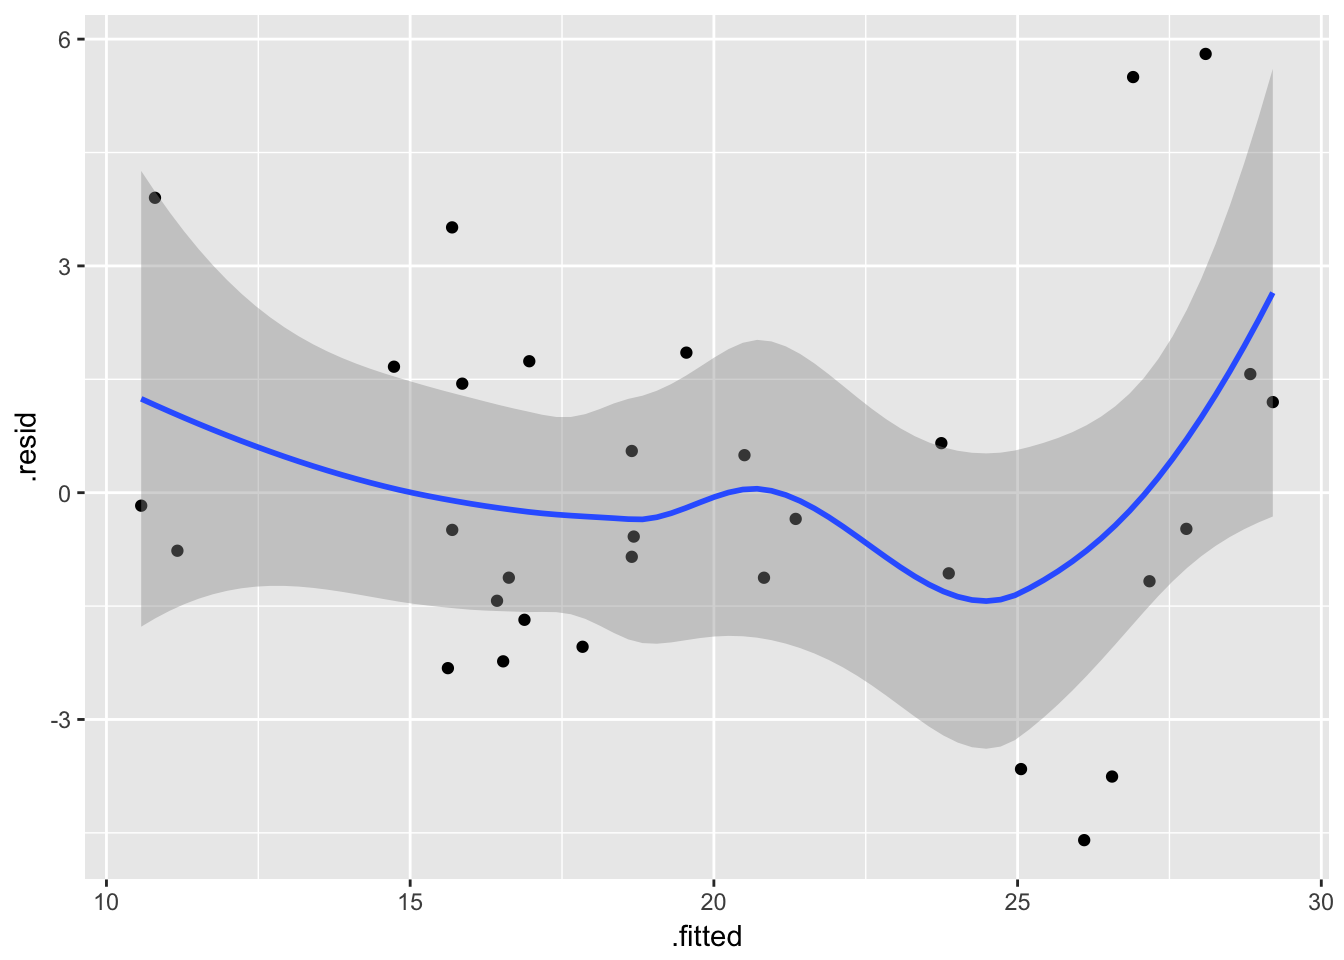
\includegraphics{graphics_files/figure-latex/unnamed-chunk-30-1.pdf}

And to facilitate the comparison between men and women we could colour
portions of the bars using \texttt{position\_stack()}:

\begin{Shaded}
\begin{Highlighting}[]
\NormalTok{reshape2}\OperatorTok{::}\NormalTok{tips }\OperatorTok\StringTok{ }
\StringTok{  }\KeywordTok{ggplot}\NormalTok{(}\KeywordTok{aes}\NormalTok{(time, tip, }\DataTypeTok{fill=}\NormalTok{sex)) }\OperatorTok{+}\StringTok{ }
\StringTok{  }\KeywordTok{stat_summary}\NormalTok{(}\DataTypeTok{geom=}\StringTok{"bar"}\NormalTok{, }\DataTypeTok{position=}\KeywordTok{position_stack}\NormalTok{()) }\OperatorTok{+}
\StringTok{  }\KeywordTok{xlab}\NormalTok{(}\StringTok{""}\NormalTok{) }\OperatorTok{+}\StringTok{ }\KeywordTok{ylab}\NormalTok{(}\StringTok{"Tip ($)"}\NormalTok{)}
\end{Highlighting}
\end{Shaded}

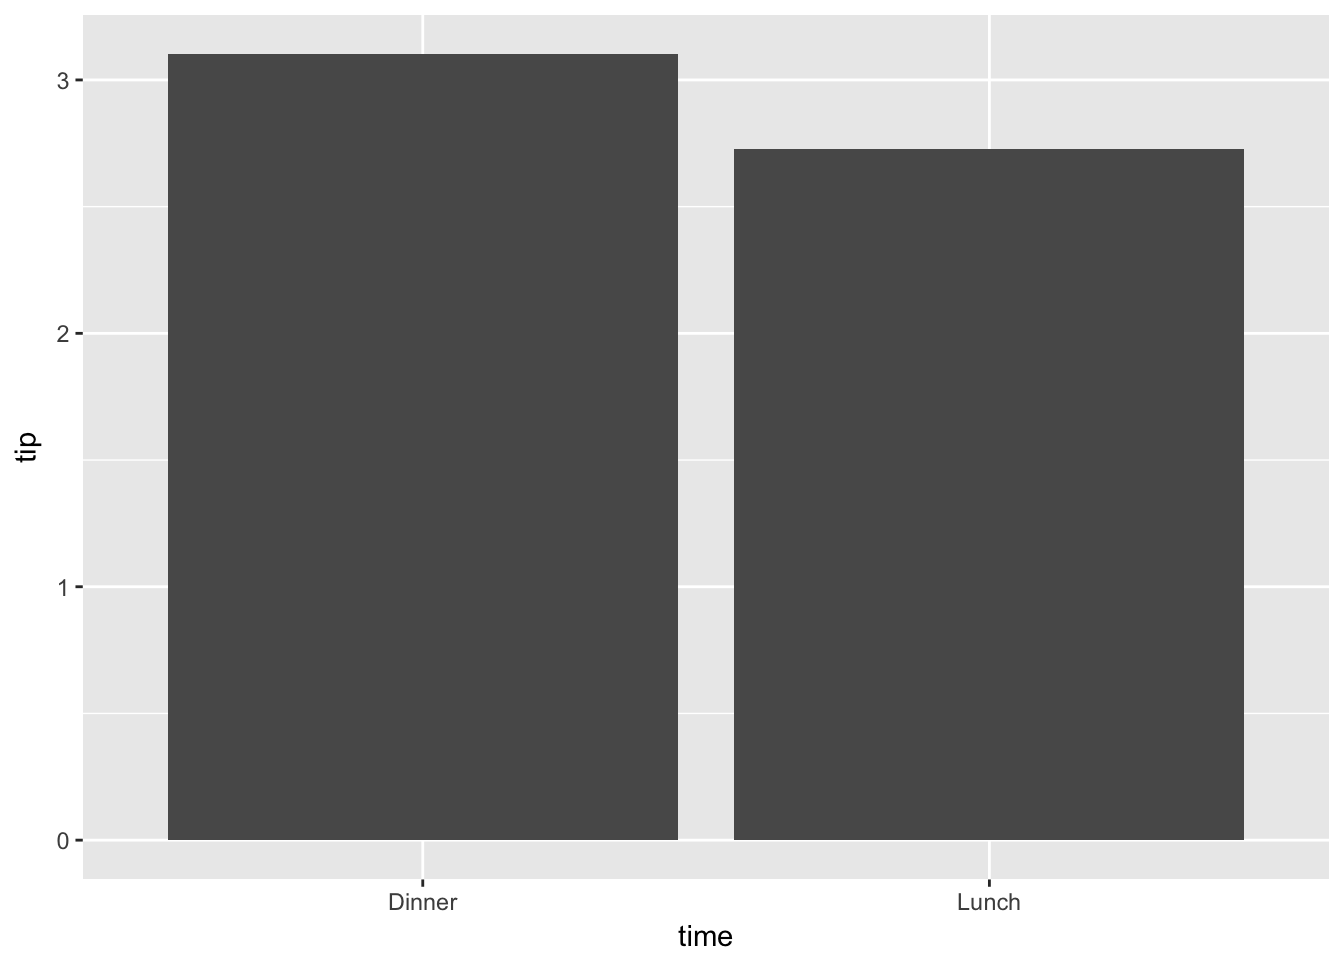
\includegraphics{graphics_files/figure-latex/unnamed-chunk-31-1.pdf}

Or to reverse the comparisons:

\begin{Shaded}
\begin{Highlighting}[]
\NormalTok{reshape2}\OperatorTok{::}\NormalTok{tips }\OperatorTok\StringTok{ }
\StringTok{  }\KeywordTok{ggplot}\NormalTok{(}\KeywordTok{aes}\NormalTok{(sex, tip, }\DataTypeTok{fill=}\NormalTok{time)) }\OperatorTok{+}\StringTok{ }
\StringTok{  }\KeywordTok{stat_summary}\NormalTok{(}\DataTypeTok{geom=}\StringTok{"bar"}\NormalTok{, }\DataTypeTok{position=}\KeywordTok{position_stack}\NormalTok{()) }\OperatorTok{+}
\StringTok{  }\KeywordTok{xlab}\NormalTok{(}\StringTok{""}\NormalTok{) }\OperatorTok{+}\StringTok{ }\KeywordTok{ylab}\NormalTok{(}\StringTok{"Tip ($)"}\NormalTok{)}
\end{Highlighting}
\end{Shaded}

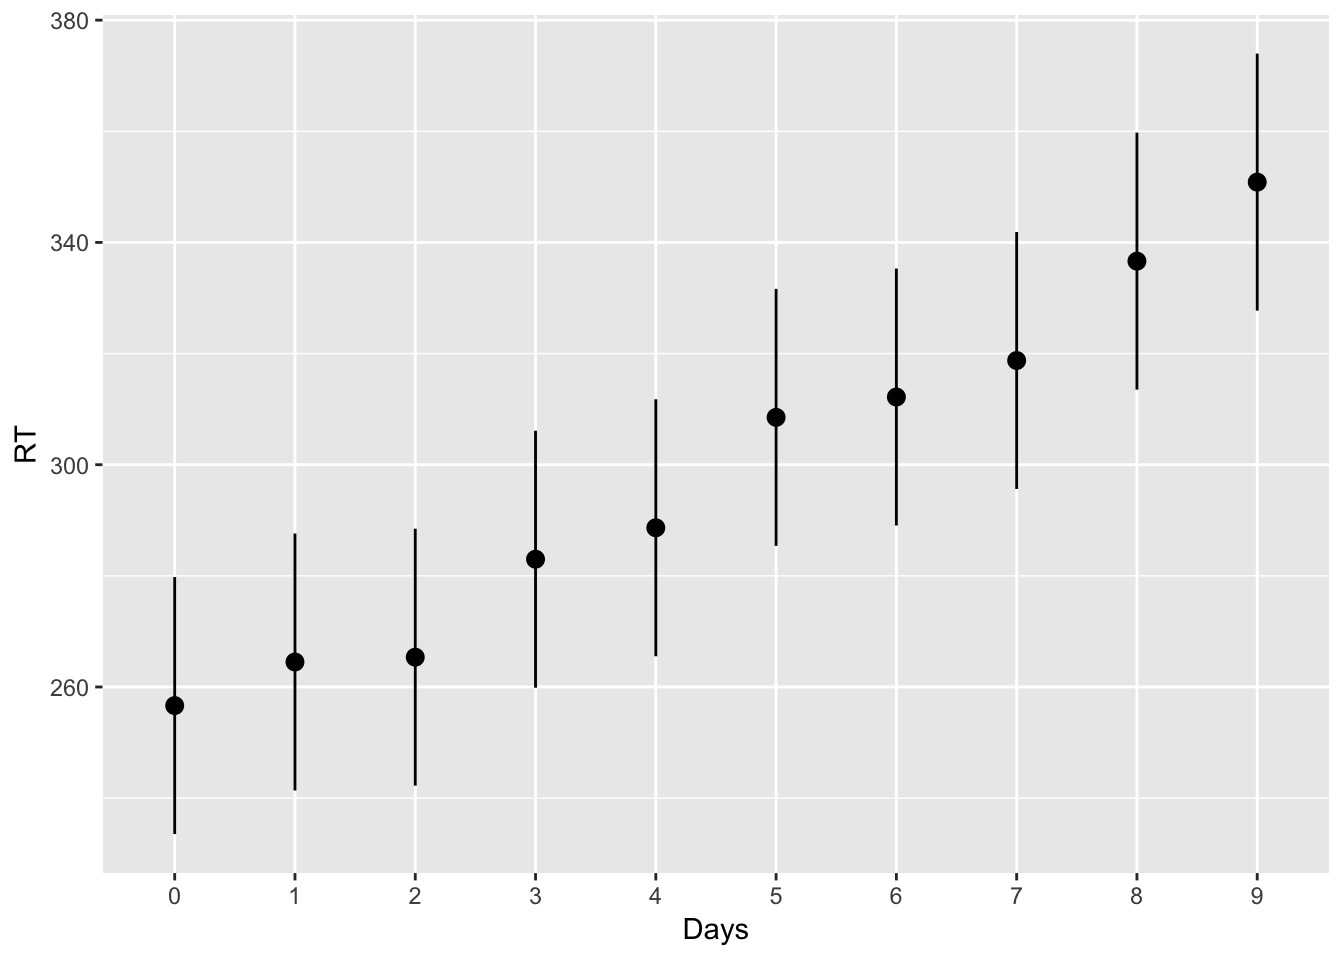
\includegraphics{graphics_files/figure-latex/unnamed-chunk-32-1.pdf}

\subsection*{\texorpdfstring{`Quick and dirty' (utility)
plots}{Quick and dirty (utility) plots}}\label{utility-plotting-functions}
\addcontentsline{toc}{subsection}{`Quick and dirty' (utility) plots}

When exploring a dataset, often useful to use built in functions or
helpers from other libraries. These help you quickly visualise
relationships, but aren't always \emph{exactly} what you need and can be
hard to customise.

\subsubsection{Distributions}\label{distributions-1}

\begin{Shaded}
\begin{Highlighting}[]
\KeywordTok{hist}\NormalTok{(mtcars}\OperatorTok{$}\NormalTok{mpg)}
\end{Highlighting}
\end{Shaded}

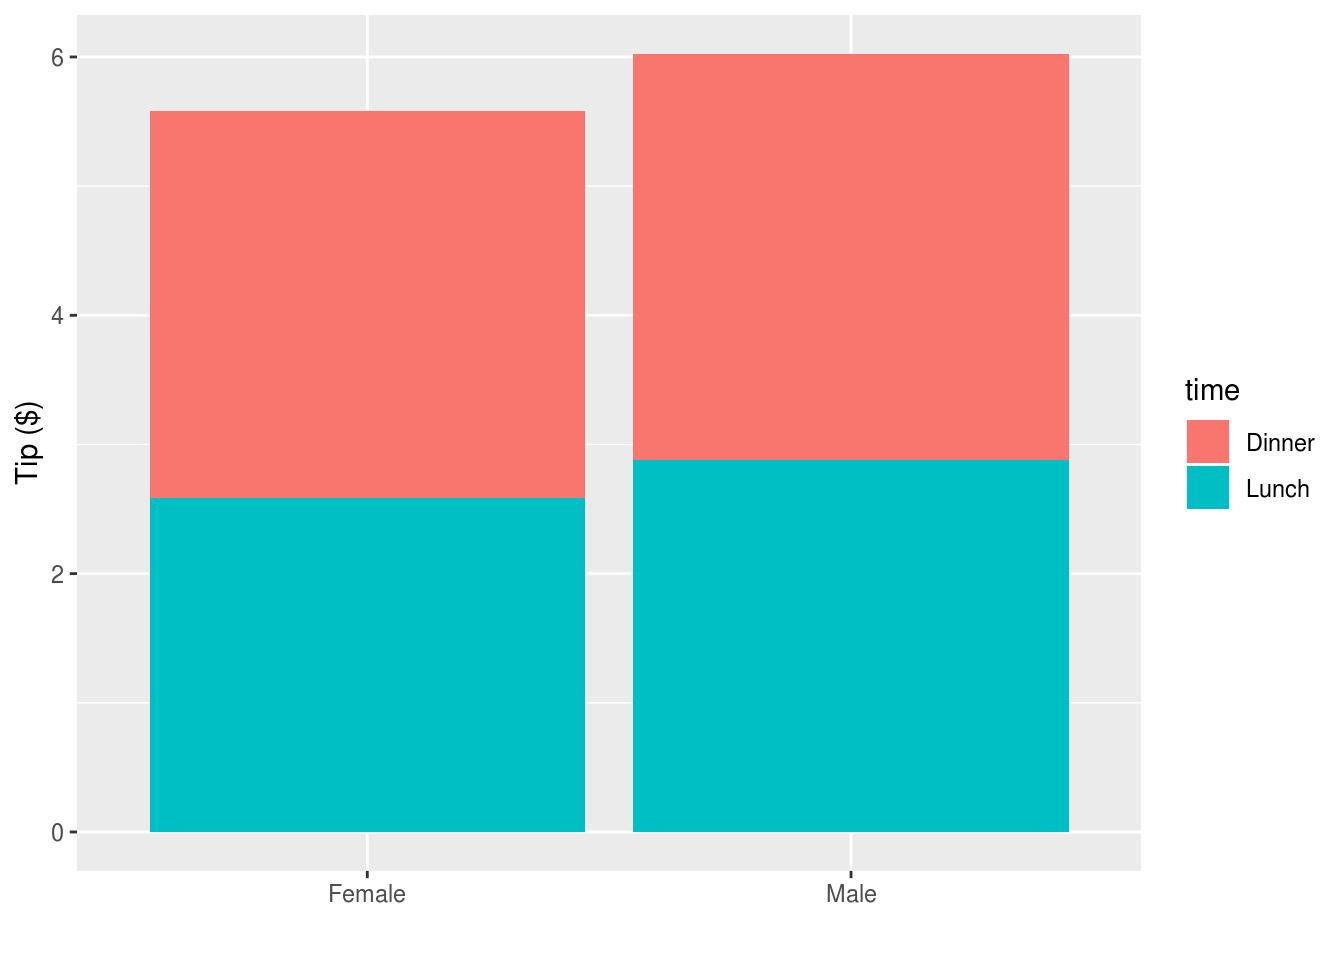
\includegraphics{graphics_files/figure-latex/unnamed-chunk-33-1.pdf}

\begin{Shaded}
\begin{Highlighting}[]
\KeywordTok{plot}\NormalTok{(}\KeywordTok{density}\NormalTok{(mtcars}\OperatorTok{$}\NormalTok{mpg))}
\end{Highlighting}
\end{Shaded}

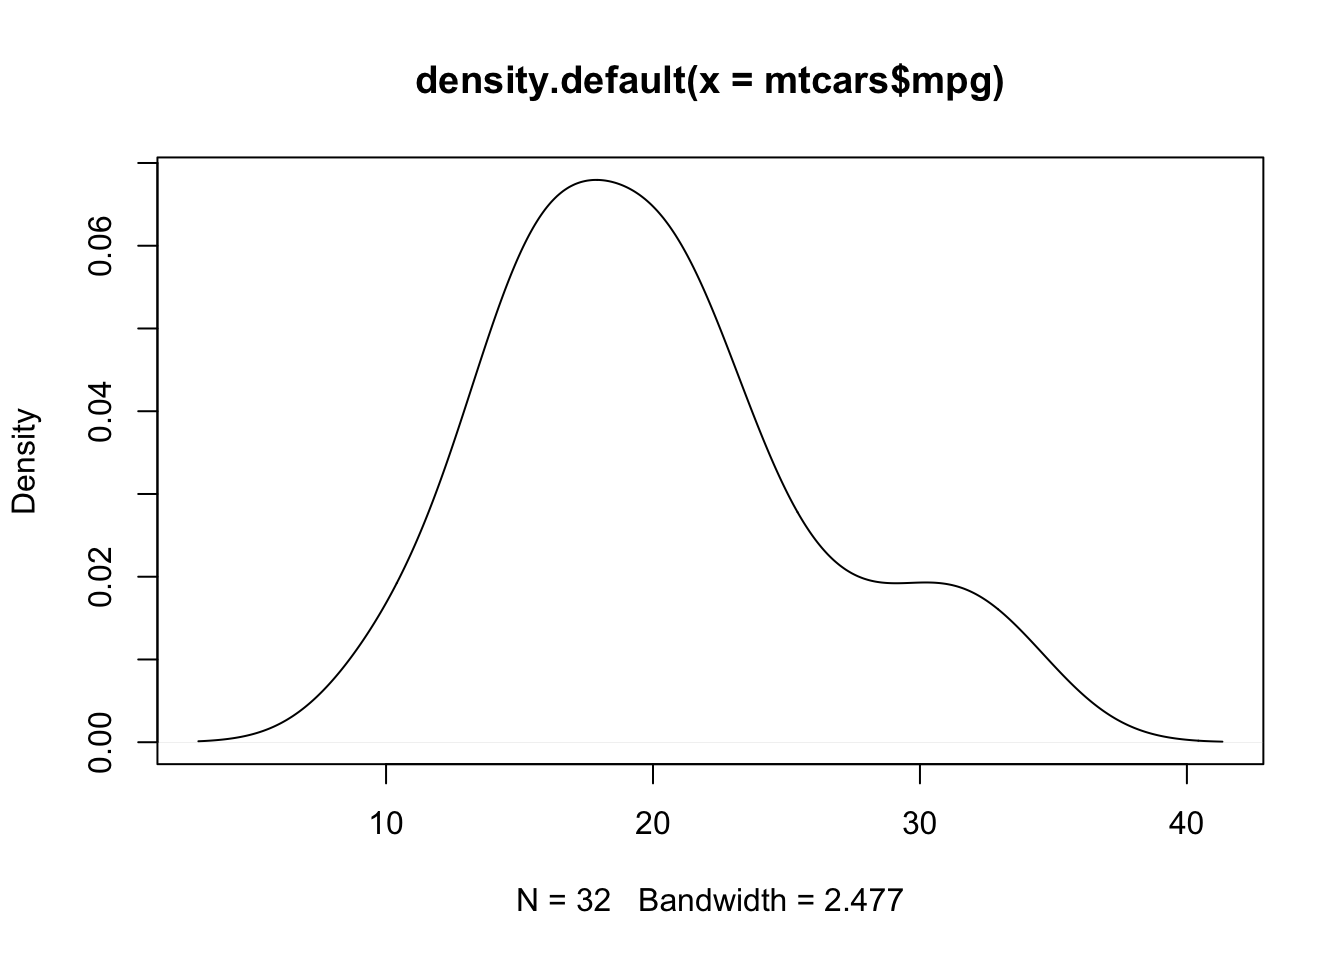
\includegraphics{graphics_files/figure-latex/unnamed-chunk-33-2.pdf}

\begin{Shaded}
\begin{Highlighting}[]
\KeywordTok{boxplot}\NormalTok{(mpg}\OperatorTok{~}\NormalTok{cyl, }\DataTypeTok{data=}\NormalTok{mtcars)}
\end{Highlighting}
\end{Shaded}

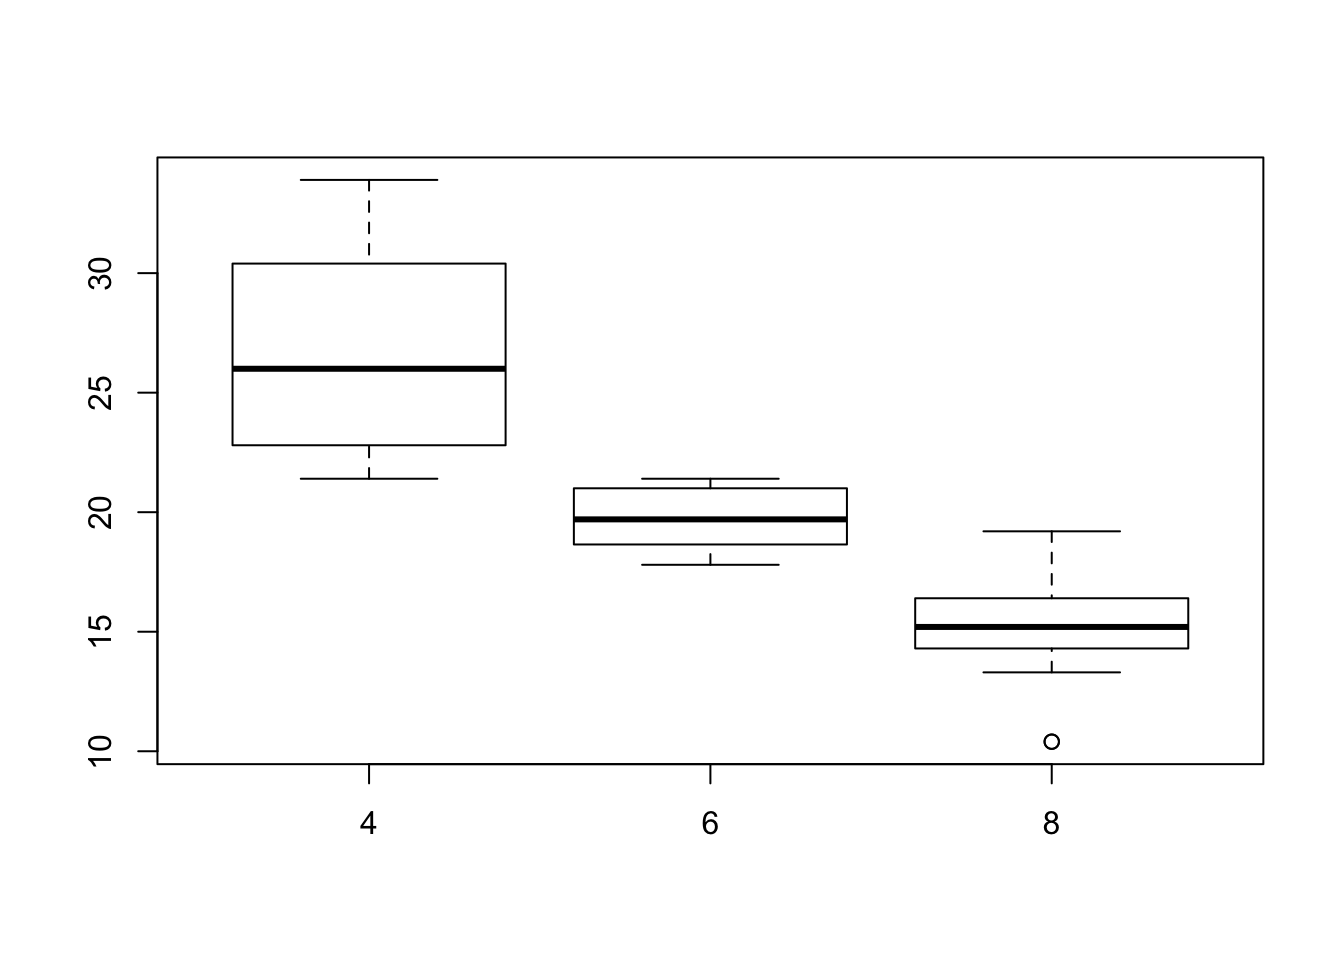
\includegraphics{graphics_files/figure-latex/unnamed-chunk-33-3.pdf}

\begin{Shaded}
\begin{Highlighting}[]
\NormalTok{Hmisc}\OperatorTok{::}\KeywordTok{hist.data.frame}\NormalTok{(mtcars)}
\end{Highlighting}
\end{Shaded}

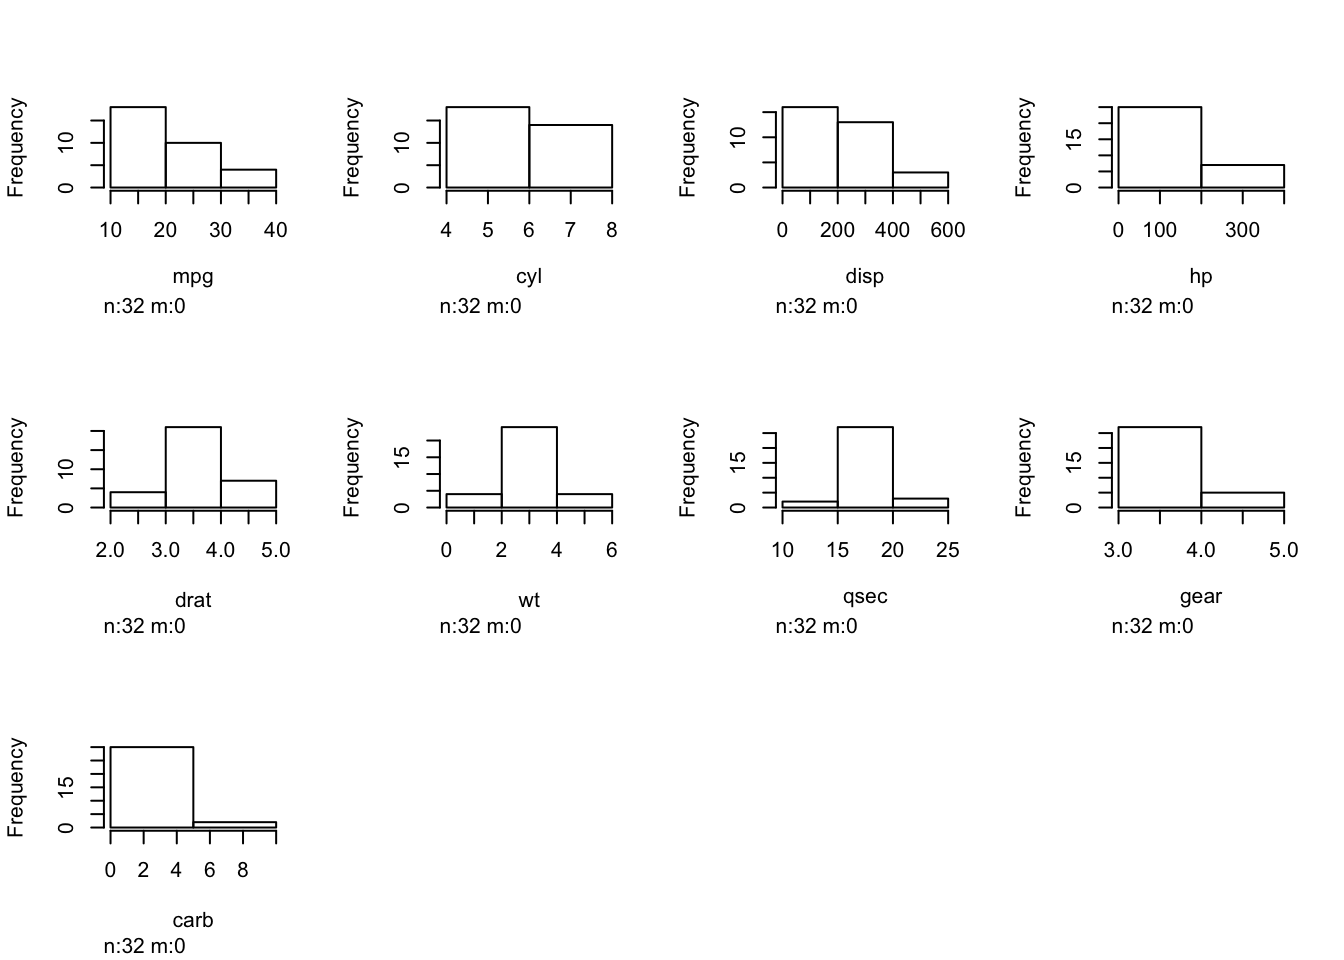
\includegraphics{graphics_files/figure-latex/unnamed-chunk-33-4.pdf}

Even for simple plots, ggplot has some useful helper functions though:

\begin{Shaded}
\begin{Highlighting}[]
\KeywordTok{qplot}\NormalTok{(mpg, }\DataTypeTok{data=}\NormalTok{mtcars, }\DataTypeTok{geom=}\StringTok{"density"}\NormalTok{) }\OperatorTok{+}\StringTok{ }\KeywordTok{xlab}\NormalTok{(}\StringTok{"Miles per gallon"}\NormalTok{)}
\end{Highlighting}
\end{Shaded}

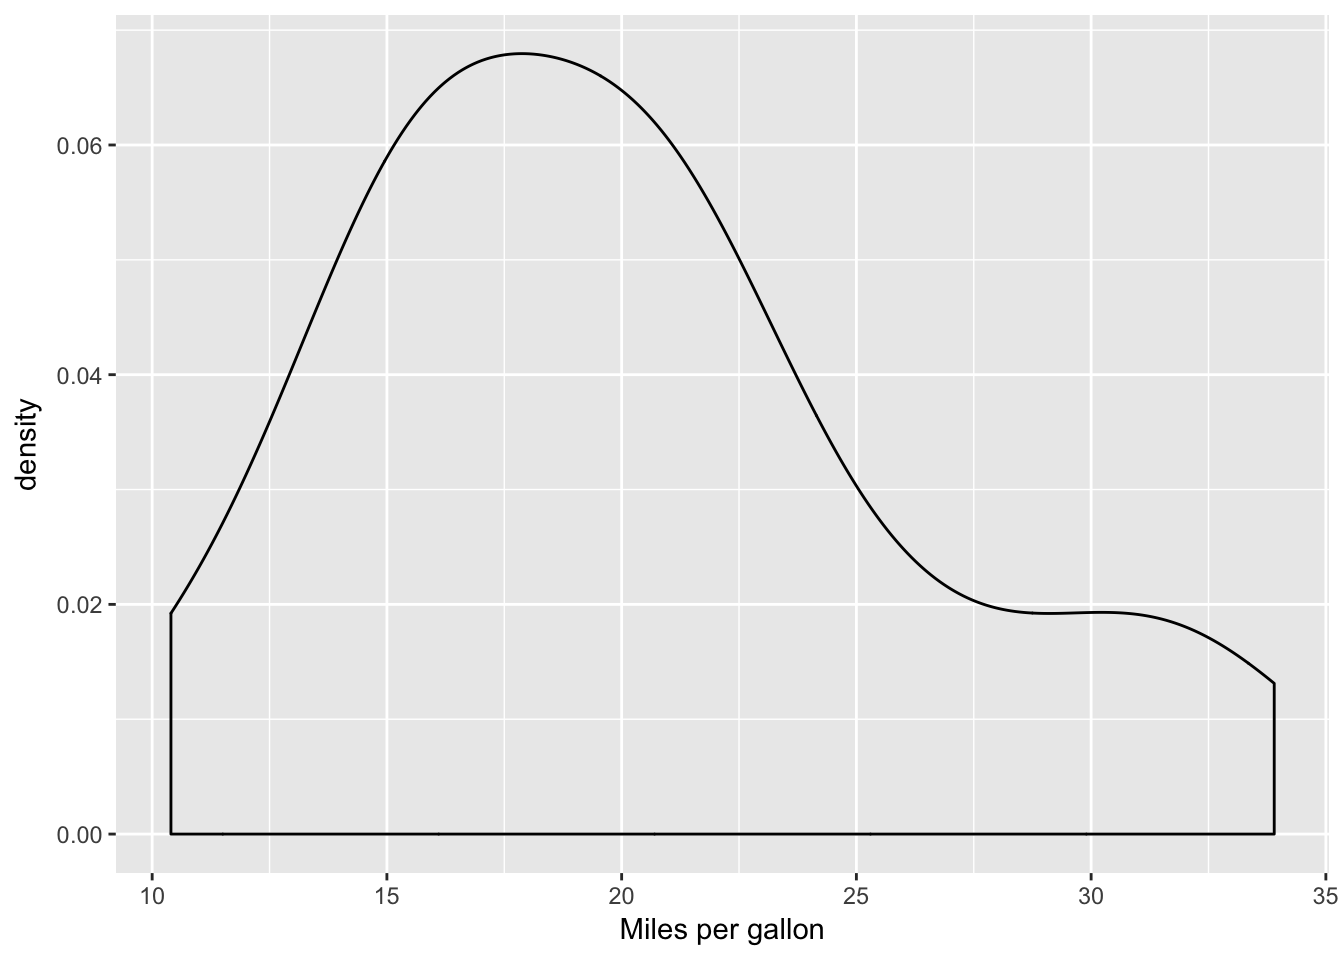
\includegraphics{graphics_files/figure-latex/unnamed-chunk-34-1.pdf}

\begin{Shaded}
\begin{Highlighting}[]
\KeywordTok{qplot}\NormalTok{(}\DataTypeTok{x=}\KeywordTok{factor}\NormalTok{(cyl), }\DataTypeTok{y=}\NormalTok{mpg, }\DataTypeTok{data=}\NormalTok{mtcars, }\DataTypeTok{geom=}\StringTok{"boxplot"}\NormalTok{) }
\end{Highlighting}
\end{Shaded}

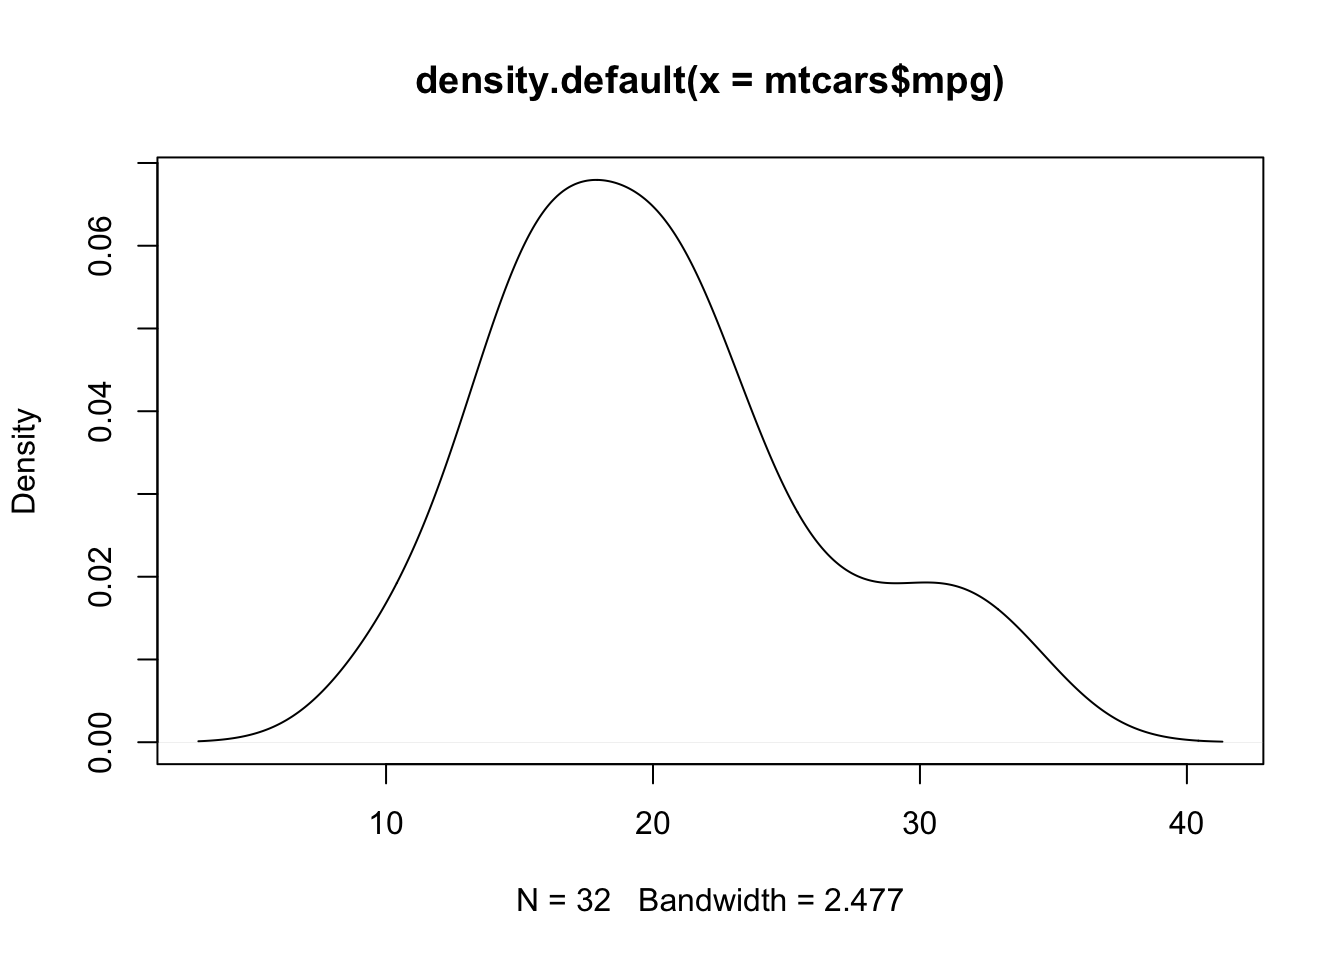
\includegraphics{graphics_files/figure-latex/unnamed-chunk-34-2.pdf}

\subsubsection{Relationships}\label{relationships-1}

\begin{Shaded}
\begin{Highlighting}[]
\KeywordTok{with}\NormalTok{(mtcars, }\KeywordTok{plot}\NormalTok{(mpg, wt))}
\end{Highlighting}
\end{Shaded}

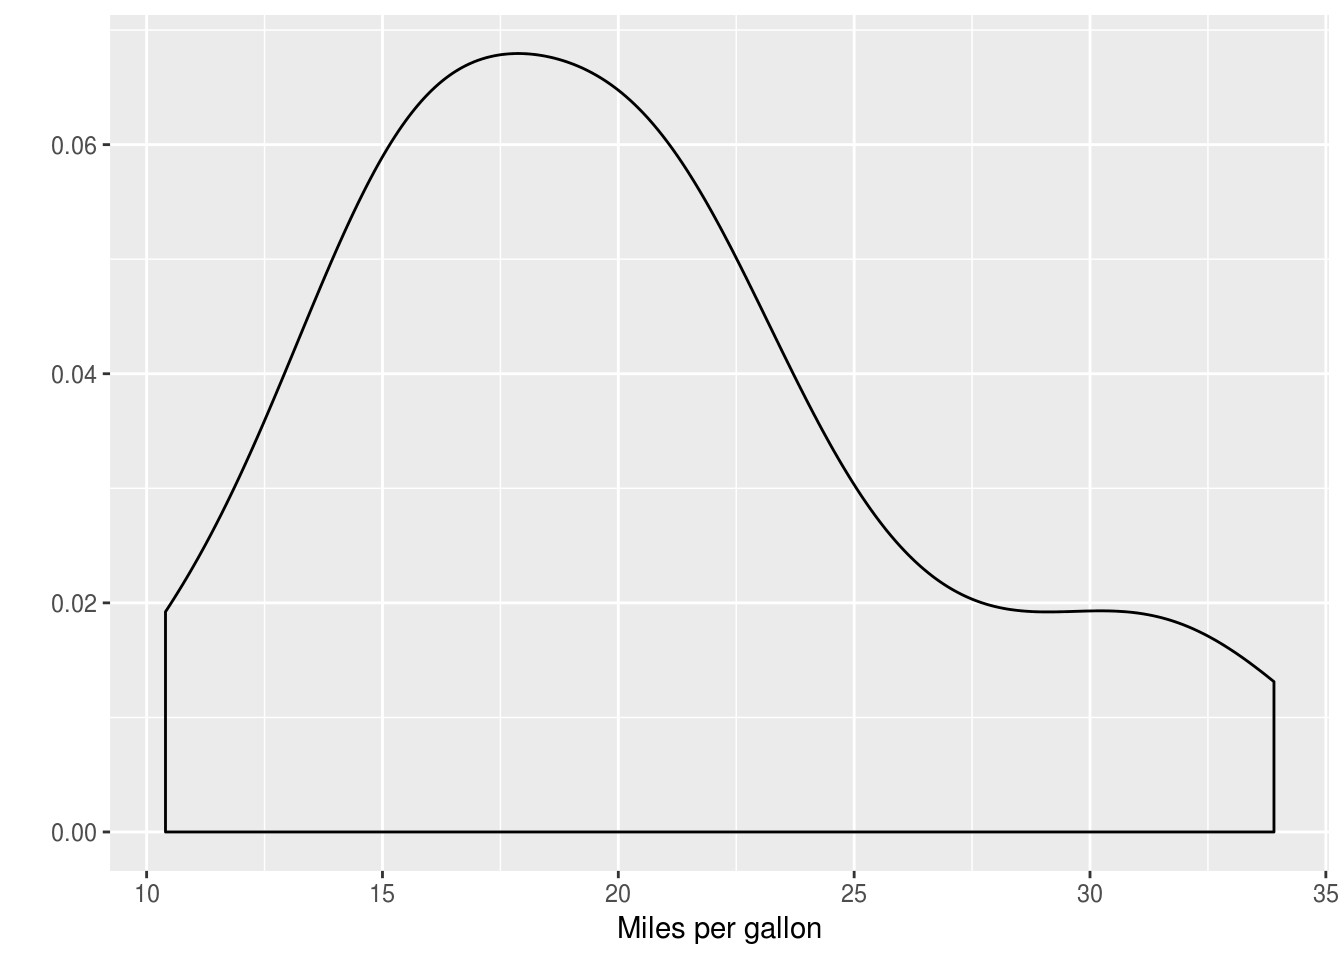
\includegraphics{graphics_files/figure-latex/unnamed-chunk-35-1.pdf}

\begin{Shaded}
\begin{Highlighting}[]
\KeywordTok{pairs}\NormalTok{(}\KeywordTok{select}\NormalTok{(mtcars, wt, disp, mpg))}
\end{Highlighting}
\end{Shaded}

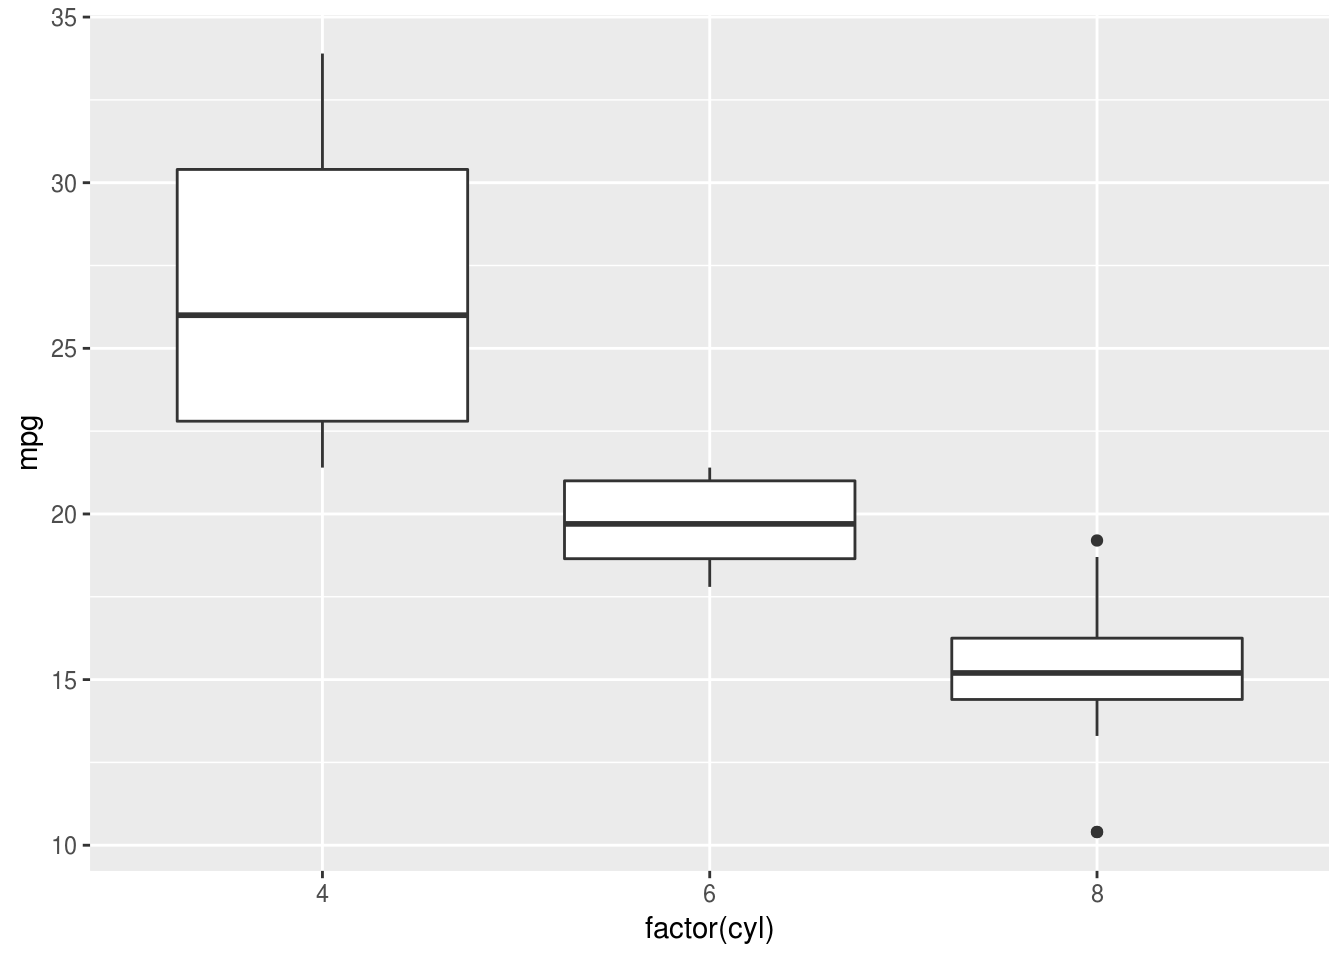
\includegraphics{graphics_files/figure-latex/unnamed-chunk-35-2.pdf}

Again, for quick plots ggplot also has useful shortcut functions:

\begin{Shaded}
\begin{Highlighting}[]
\KeywordTok{qplot}\NormalTok{(mpg, wt, }\DataTypeTok{color=}\KeywordTok{factor}\NormalTok{(cyl), }\DataTypeTok{data =}\NormalTok{ mtcars)}
\end{Highlighting}
\end{Shaded}

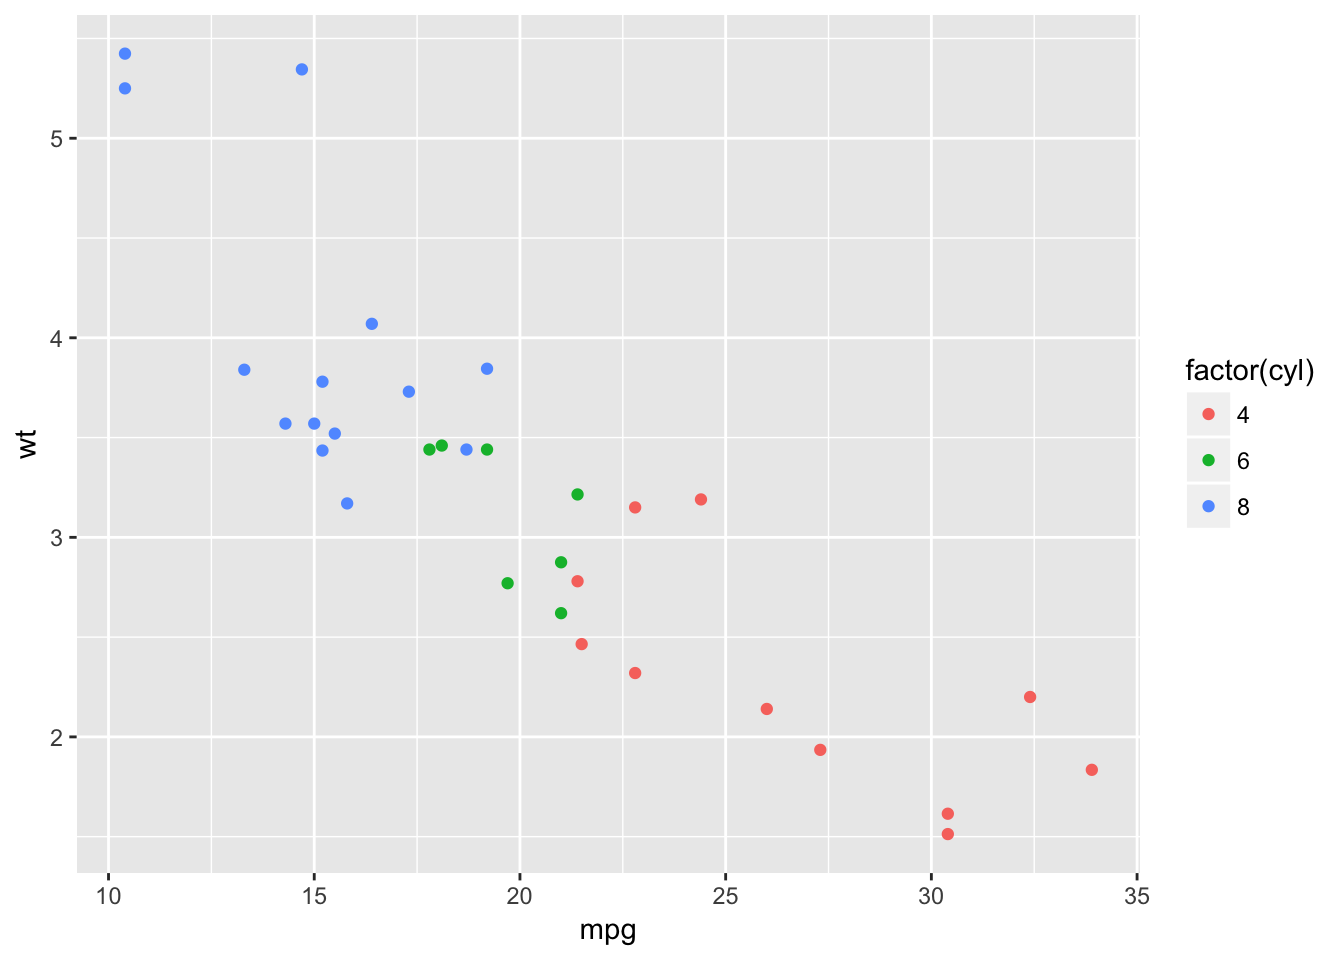
\includegraphics{graphics_files/figure-latex/unnamed-chunk-36-1.pdf}

\subsubsection{Quantities}\label{quantities}

I don't think the base R plots are that convenient here.
\texttt{ggplot2::} and the \texttt{stat\_summary()} function makes life
much simpler:

\begin{Shaded}
\begin{Highlighting}[]
\KeywordTok{ggplot}\NormalTok{(mtcars, }\KeywordTok{aes}\NormalTok{(}\KeywordTok{factor}\NormalTok{(cyl), mpg)) }\OperatorTok{+}\StringTok{ }
\StringTok{  }\KeywordTok{stat_summary}\NormalTok{(}\DataTypeTok{geom=}\StringTok{"bar"}\NormalTok{)}
\end{Highlighting}
\end{Shaded}

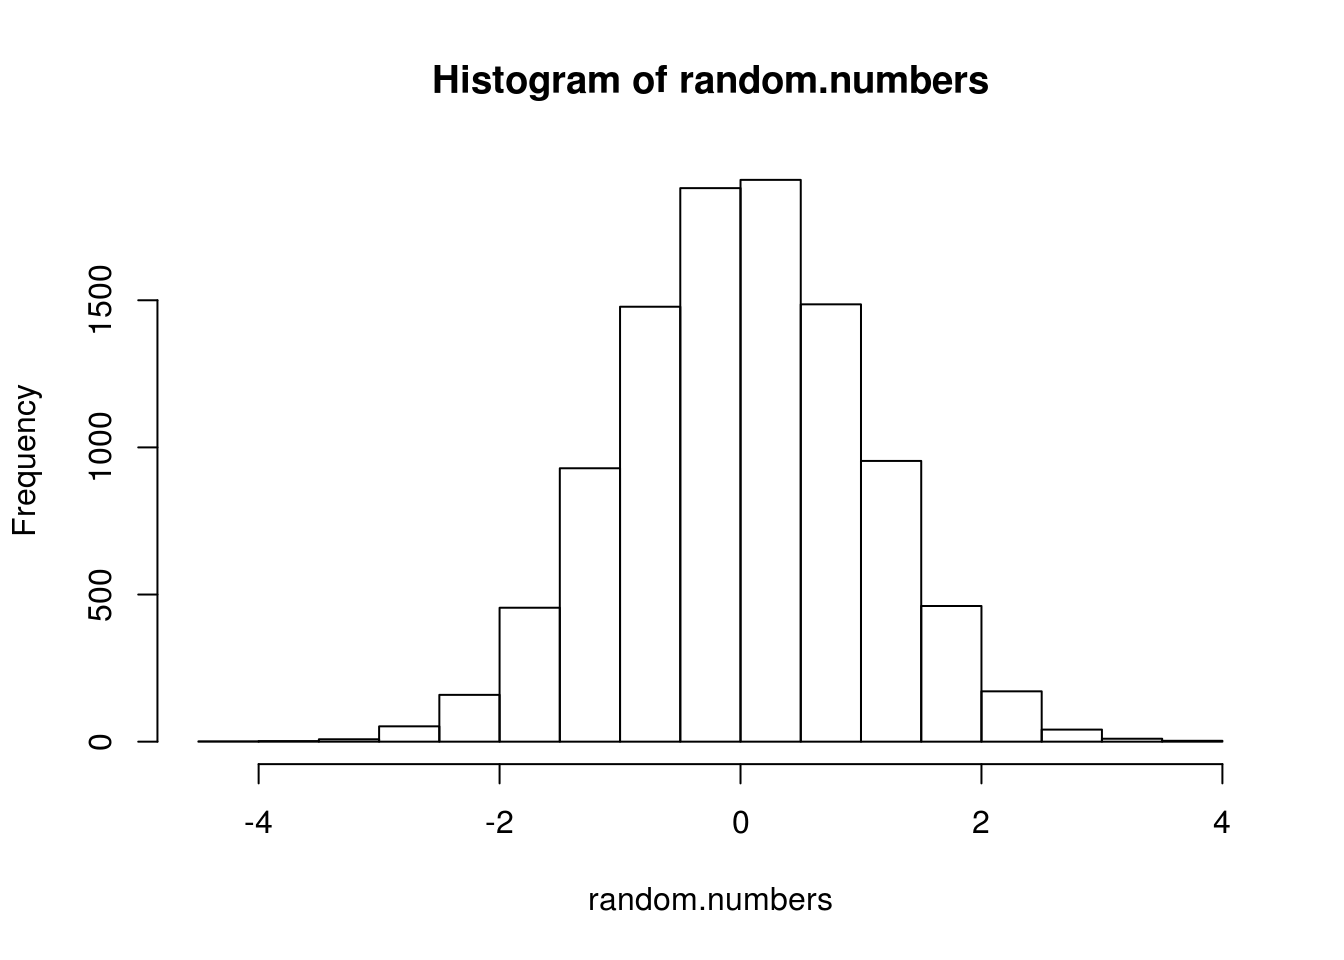
\includegraphics{graphics_files/figure-latex/unnamed-chunk-37-1.pdf}

And if you are plotting quantities, as disussed above, showing a range
is sensible (a boxplot would also fill both definitions):

\begin{Shaded}
\begin{Highlighting}[]
\KeywordTok{ggplot}\NormalTok{(mtcars, }\KeywordTok{aes}\NormalTok{(}\KeywordTok{factor}\NormalTok{(cyl), mpg)) }\OperatorTok{+}\StringTok{ }
\StringTok{  }\KeywordTok{stat_summary}\NormalTok{(}\DataTypeTok{geom=}\StringTok{"pointrange"}\NormalTok{)}
\end{Highlighting}
\end{Shaded}

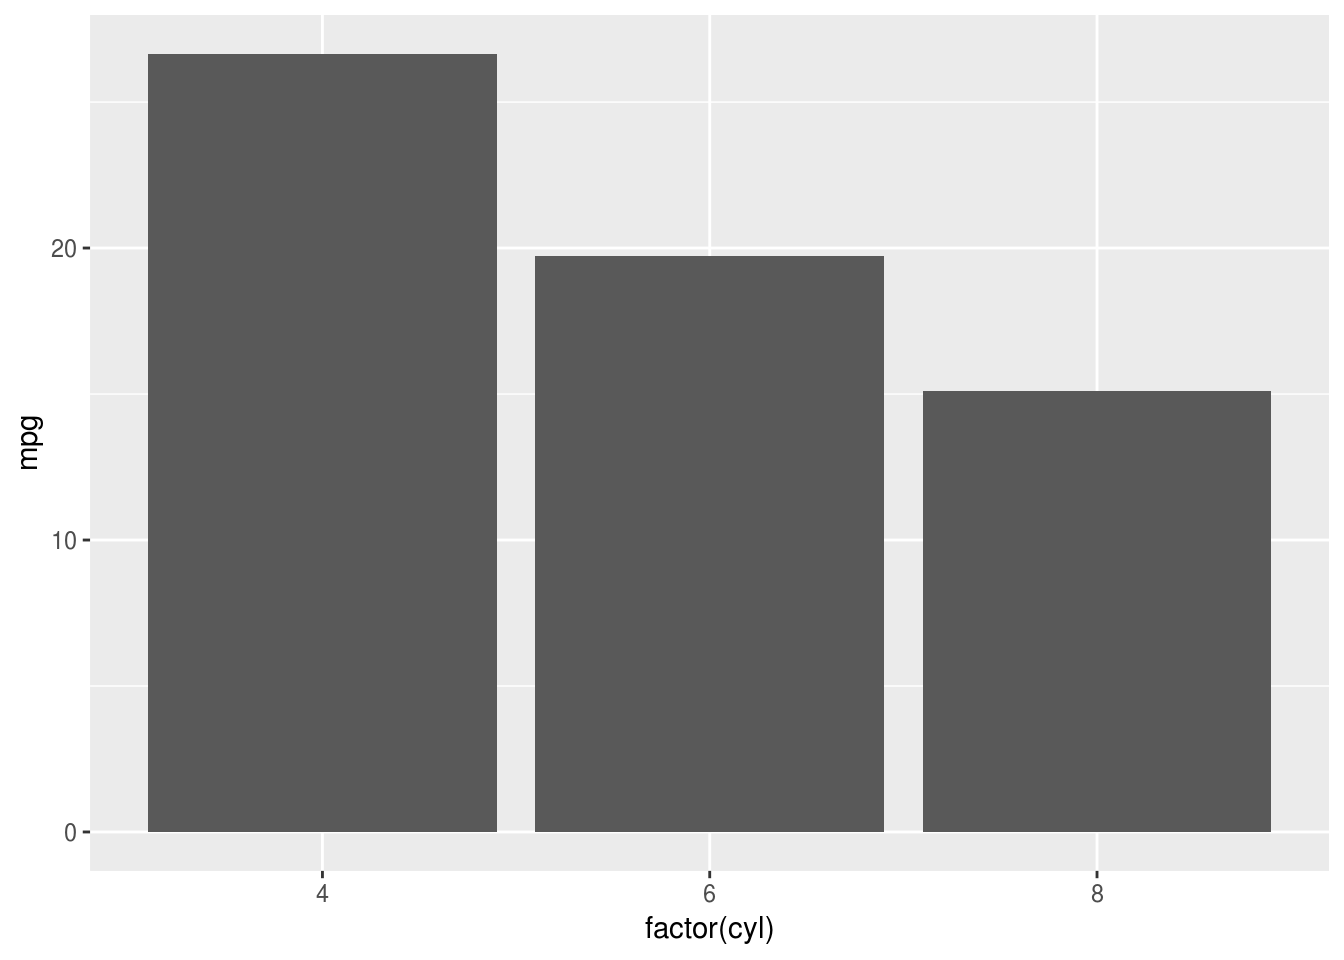
\includegraphics{graphics_files/figure-latex/unnamed-chunk-38-1.pdf}

\subsection*{Tricks with ggplot}\label{ggplot-details}
\addcontentsline{toc}{subsection}{Tricks with ggplot}

\hypertarget{facetting-plots}{\subsubsection*{More ways to facet a
plot}\label{facetting-plots}}
\addcontentsline{toc}{subsubsection}{More ways to facet a plot}

Facets are ways to repeat a plot for each level of another variable.
\texttt{ggplot} has two ways of defining and displaying facets:

\begin{itemize}
\tightlist
\item
  As a list of plots, using \texttt{facet\_wrap}.
\item
  As a grid or matrix of plots, using \texttt{facet\_grid()}.
\end{itemize}

Examples of both are shown below, using the following plot as a starting
point:

\begin{Shaded}
\begin{Highlighting}[]
\NormalTok{base.plot <-}\StringTok{ }\KeywordTok{ggplot}\NormalTok{(mtcars, }\KeywordTok{aes}\NormalTok{(mpg, wt)) }\OperatorTok{+}\StringTok{ }\KeywordTok{geom_point}\NormalTok{()}
\NormalTok{base.plot}
\end{Highlighting}
\end{Shaded}

\includegraphics{graphics-ggplot-extras_files/figure-latex/unnamed-chunk-2-1.pdf}

\subsubsection*{\texorpdfstring{\texttt{facet\_wrap}}{facet\_wrap}}\label{facet_wrap}
\addcontentsline{toc}{subsubsection}{\texttt{facet\_wrap}}

If we want one facet we just type the tilde (\texttt{\textasciitilde{}})
symbol and then the name of the variable. This is like typing the right
hand side of a \href{formulae}{formula for a regression model}:

\begin{Shaded}
\begin{Highlighting}[]
\NormalTok{base.plot }\OperatorTok{+}\StringTok{ }\KeywordTok{facet_wrap}\NormalTok{(}\OperatorTok{~}\NormalTok{cyl)}
\end{Highlighting}
\end{Shaded}

\includegraphics{graphics-ggplot-extras_files/figure-latex/unnamed-chunk-3-1.pdf}

If we want two facets we extend the formula, using the \texttt{+} sign:

\begin{Shaded}
\begin{Highlighting}[]
\NormalTok{base.plot }\OperatorTok{+}\StringTok{ }\KeywordTok{facet_wrap}\NormalTok{(}\OperatorTok{~}\NormalTok{cyl}\OperatorTok{+}\NormalTok{am)}
\end{Highlighting}
\end{Shaded}

\includegraphics{graphics-ggplot-extras_files/figure-latex/unnamed-chunk-4-1.pdf}

Note, the order of variables in the formula makes a difference:

\begin{Shaded}
\begin{Highlighting}[]
\NormalTok{base.plot }\OperatorTok{+}\StringTok{ }\KeywordTok{facet_wrap}\NormalTok{(}\OperatorTok{~}\NormalTok{am}\OperatorTok{+}\NormalTok{cyl)}
\end{Highlighting}
\end{Shaded}

\includegraphics{graphics-ggplot-extras_files/figure-latex/unnamed-chunk-5-1.pdf}

\subsubsection*{\texorpdfstring{\texttt{facet\_grid}}{facet\_grid}}\label{facet_grid}
\addcontentsline{toc}{subsubsection}{\texttt{facet\_grid}}

With one variable \texttt{facet\_grid} produces similar output. Note the
\texttt{.} (period) on the left hand side of the formula now to make
explicit we only have one variable, and we want it on the x axis:

\begin{Shaded}
\begin{Highlighting}[]
\NormalTok{base.plot }\OperatorTok{+}\StringTok{ }\KeywordTok{facet_grid}\NormalTok{(.}\OperatorTok{~}\NormalTok{cyl)}
\end{Highlighting}
\end{Shaded}

\includegraphics{graphics-ggplot-extras_files/figure-latex/unnamed-chunk-6-1.pdf}

We can flip the facets around by putting the \texttt{cyl} variable on
the left hand side of the \texttt{\textasciitilde{}}:

\begin{Shaded}
\begin{Highlighting}[]
\NormalTok{base.plot }\OperatorTok{+}\StringTok{ }\KeywordTok{facet_grid}\NormalTok{(cyl}\OperatorTok{~}\NormalTok{.)}
\end{Highlighting}
\end{Shaded}

\includegraphics{graphics-ggplot-extras_files/figure-latex/unnamed-chunk-7-1.pdf}

And \texttt{facet\_grid} can also create facets for two or more
variables:

\begin{Shaded}
\begin{Highlighting}[]
\NormalTok{base.plot }\OperatorTok{+}\StringTok{ }\KeywordTok{facet_grid}\NormalTok{(am}\OperatorTok{~}\NormalTok{cyl)}
\end{Highlighting}
\end{Shaded}

\includegraphics{graphics-ggplot-extras_files/figure-latex/unnamed-chunk-8-1.pdf}

Here the labelling and the arrangement of plots is perhaps nicer because
it is clearer that plots for \texttt{cyl} are arrange left to right, and
for \texttt{am} they are top to bottom.

\subsubsection*{Combining separate plots in a
grid}\label{combining-plots}
\addcontentsline{toc}{subsubsection}{Combining separate plots in a grid}

Note that combining separate plots in a grid is different from
\protect\hyperlink{facetting-plots}{facetting}, and it may be you want
that instead.

If you really want to combine several plots, the \texttt{gridExtra} and
\texttt{cowplot} packages can be helpful. This is the code from the
\protect\hyperlink{layered-graphics}{example in the graphics section},
which may be a useful starting point:

\begin{Shaded}
\begin{Highlighting}[]
\NormalTok{comparison <-}\StringTok{ }\KeywordTok{ggplot}\NormalTok{(mtcars, }\KeywordTok{aes}\NormalTok{(}\KeywordTok{factor}\NormalTok{(cyl), mpg)) }\OperatorTok{+}\StringTok{ }\KeywordTok{geom_boxplot}\NormalTok{() }\OperatorTok{+}\StringTok{  }\KeywordTok{ggtitle}\NormalTok{(}\StringTok{"Comparison"}\NormalTok{)}
\NormalTok{relationships <-}\StringTok{ }\KeywordTok{ggplot}\NormalTok{(mtcars, }\KeywordTok{aes}\NormalTok{(wt, mpg, }\DataTypeTok{color=}\KeywordTok{factor}\NormalTok{(gear))) }\OperatorTok{+}\StringTok{ }\KeywordTok{geom_point}\NormalTok{() }\OperatorTok{+}\StringTok{ }\KeywordTok{ggtitle}\NormalTok{(}\StringTok{"Relationship"}\NormalTok{)}
\NormalTok{distributions <-}\StringTok{ }\KeywordTok{ggplot}\NormalTok{(mtcars, }\KeywordTok{aes}\NormalTok{(mpg, }\DataTypeTok{color=}\KeywordTok{factor}\NormalTok{(gear))) }\OperatorTok{+}\StringTok{ }\KeywordTok{geom_density}\NormalTok{() }\OperatorTok{+}\StringTok{ }\KeywordTok{ggtitle}\NormalTok{(}\StringTok{"Distribution"}\NormalTok{)}
\NormalTok{composition <-}\StringTok{ }\KeywordTok{ggplot}\NormalTok{(mtcars, }\KeywordTok{aes}\NormalTok{(}\KeywordTok{factor}\NormalTok{(cyl), }\DataTypeTok{fill =} \KeywordTok{factor}\NormalTok{(gear))) }\OperatorTok{+}\StringTok{ }\KeywordTok{geom_bar}\NormalTok{() }\OperatorTok{+}\StringTok{ }\KeywordTok{ggtitle}\NormalTok{(}\StringTok{"Composition"}\NormalTok{)}
\NormalTok{mm <-}\StringTok{ }\KeywordTok{theme}\NormalTok{(}\DataTypeTok{plot.margin=}\KeywordTok{unit}\NormalTok{(}\KeywordTok{rep}\NormalTok{(}\FloatTok{1.5}\NormalTok{,}\DecValTok{4}\NormalTok{), }\StringTok{"line"}\NormalTok{))}
\NormalTok{gridExtra}\OperatorTok{::}\KeywordTok{grid.arrange}\NormalTok{(relationships}\OperatorTok{+}\NormalTok{mm, distributions}\OperatorTok{+}\NormalTok{mm, comparison}\OperatorTok{+}\NormalTok{mm, composition}\OperatorTok{+}\NormalTok{mm, }\DataTypeTok{ncol=}\DecValTok{2}\NormalTok{)}
\end{Highlighting}
\end{Shaded}

\includegraphics{graphics-ggplot-extras_files/figure-latex/unnamed-chunk-9-1.pdf}

\subsection*{Exporting for print}\label{exporting-graphics}
\addcontentsline{toc}{subsection}{Exporting for print}

To export ggplot graphics you can use the \texttt{ggsave()} function:

\begin{Shaded}
\begin{Highlighting}[]

\KeywordTok{ggplot}\NormalTok{(mtcars, }\KeywordTok{aes}\NormalTok{(wt, mpg)) }\OperatorTok{+}\StringTok{ }\KeywordTok{geom_point}\NormalTok{()}
\KeywordTok{ggsave}\NormalTok{(}\DataTypeTok{filename =} \StringTok{"myplot.pdf"}\NormalTok{)}
\end{Highlighting}
\end{Shaded}

See the \href{http://ggplot2.tidyverse.org/reference/ggsave.html}{ggplot
docs on exporting} or page
\href{https://ase.tufts.edu/bugs/guide/assets/R\%20Graphics\%20Cookbook.pdf}{323
of the R Graphics Cookbook} for lots more detail.

\section{Example datasets}\label{example-datasets}

The

\part{Models}\label{part-models}

\hypertarget{common-inferential-stats}{\section{Common inferential
statistics}\label{common-inferential-stats}}

R has simple functions for common inferential statistics like
Chi\textsuperscript{2}, t-tests, correlations and many more. This
section is by no means exhaustive, but covers
\protect\hyperlink{crosstabs}{statistics for crosstabulations},
\protect\hyperlink{t-tests}{differences in means}, and
\protect\hyperlink{correlations}{linear correlation}.

For more on non-parametric statistics
\href{http://www.statmethods.net/stats/nonparametric.html}{this page on
the statmethods site} is a useful guide.

The
\href{http://finzi.psych.upenn.edu/R/library/coin/doc/coin.pdf}{\texttt{coin::}
package} implements many resampling tests, which can also be useful when
assumptions of parametric tests are not valid.
\href{http://www.statmethods.net/stats/resampling.html}{See this intro
to resampling statistics}.

\hypertarget{crosstabs}{\subsection*{\texorpdfstring{Crosstabulations
and
\(\chi^2\)}{Crosstabulations and \textbackslash{}chi\^{}2}}\label{crosstabs}}
\addcontentsline{toc}{subsection}{Crosstabulations and \(\chi^2\)}

We saw in a previous section \protect\hyperlink{frequency-tables}{how to
create a frequency table of one or more variables}. Using that previous
example, assume we already have a crosstabulation of \texttt{age} and
\texttt{prefers}

\begin{Shaded}
\begin{Highlighting}[]
\NormalTok{lego.table}
\NormalTok{##          prefers}
\NormalTok{## age       duplo lego}
\NormalTok{##   4 years    38   20}
\NormalTok{##   6 years    12   30}
\end{Highlighting}
\end{Shaded}

We can easily run the inferential \(\chi^2\) (sometimes spelled ``chi'',
but pronounced ``kai''-squared) test on this table:

\begin{Shaded}
\begin{Highlighting}[]
\NormalTok{lego.test <-}\StringTok{ }\KeywordTok{chisq.test}\NormalTok{(lego.table)}
\NormalTok{lego.test}
\NormalTok{## }
\NormalTok{##  Pearson's Chi-squared test with Yates' continuity correction}
\NormalTok{## }
\NormalTok{## data:  lego.table}
\NormalTok{## X-squared = 11.864, df = 1, p-value = 0.0005724}
\end{Highlighting}
\end{Shaded}

Note that we can access each number in this output individually because
the \texttt{chisq.test} function returns \protect\hyperlink{lists}{a
list}. We do this by using the \texttt{\$} syntax:

\begin{Shaded}
\begin{Highlighting}[]
\CommentTok{# access the chi2 value alone}
\NormalTok{lego.test}\OperatorTok{$}\NormalTok{statistic}
\NormalTok{## X-squared }
\NormalTok{##  11.86371}
\end{Highlighting}
\end{Shaded}

Even nicer, you can use an R package to write up your results for you in
APA format!

\begin{Shaded}
\begin{Highlighting}[]
\KeywordTok{library}\NormalTok{(apa)}
\KeywordTok{apa}\NormalTok{(lego.test, }\DataTypeTok{print_n=}\NormalTok{T)}
\NormalTok{## [1] "$\textbackslash{}\textbackslash{}chi^2$(1, n = 100) = 11.86, *p* < .001"}
\end{Highlighting}
\end{Shaded}

\protect\hyperlink{apa-output}{See more on automatically displaying
statistics in APA format}

\subsubsection*{Three-way tables}\label{three-way-tables}
\addcontentsline{toc}{subsubsection}{Three-way tables}

You can also use \texttt{table()} or \texttt{xtabs()} to get 3-way
tables of frequencies (\texttt{xtabs} is probably better for this than
\texttt{table}).

For example, using the \texttt{mtcars} dataset we create a 3-way table,
and then convert the result to a dataframe. This means we can print the
table nicely in RMarkdown using the \texttt{pander.table()} function, or
process it further (e.g.~by \protect\hyperlink{sorting}{sorting} or
\protect\hyperlink{reshaping}{reshaping} it).

\begin{Shaded}
\begin{Highlighting}[]
\KeywordTok{xtabs}\NormalTok{(}\OperatorTok{~}\NormalTok{am}\OperatorTok{+}\NormalTok{gear}\OperatorTok{+}\NormalTok{cyl, mtcars) }\OperatorTok
\StringTok{  }\KeywordTok{as_data_frame}\NormalTok{() }\OperatorTok\StringTok{ }
\StringTok{  }\KeywordTok{pander}\NormalTok{()}
\end{Highlighting}
\end{Shaded}

\begin{longtable}[]{@{}cccc@{}}
\toprule
\begin{minipage}[b]{0.06\columnwidth}\centering\strut
am\strut
\end{minipage} & \begin{minipage}[b]{0.09\columnwidth}\centering\strut
gear\strut
\end{minipage} & \begin{minipage}[b]{0.07\columnwidth}\centering\strut
cyl\strut
\end{minipage} & \begin{minipage}[b]{0.07\columnwidth}\centering\strut
n\strut
\end{minipage}\tabularnewline
\midrule
\endhead
\begin{minipage}[t]{0.06\columnwidth}\centering\strut
0\strut
\end{minipage} & \begin{minipage}[t]{0.09\columnwidth}\centering\strut
3\strut
\end{minipage} & \begin{minipage}[t]{0.07\columnwidth}\centering\strut
4\strut
\end{minipage} & \begin{minipage}[t]{0.07\columnwidth}\centering\strut
1\strut
\end{minipage}\tabularnewline
\begin{minipage}[t]{0.06\columnwidth}\centering\strut
1\strut
\end{minipage} & \begin{minipage}[t]{0.09\columnwidth}\centering\strut
3\strut
\end{minipage} & \begin{minipage}[t]{0.07\columnwidth}\centering\strut
4\strut
\end{minipage} & \begin{minipage}[t]{0.07\columnwidth}\centering\strut
0\strut
\end{minipage}\tabularnewline
\begin{minipage}[t]{0.06\columnwidth}\centering\strut
0\strut
\end{minipage} & \begin{minipage}[t]{0.09\columnwidth}\centering\strut
4\strut
\end{minipage} & \begin{minipage}[t]{0.07\columnwidth}\centering\strut
4\strut
\end{minipage} & \begin{minipage}[t]{0.07\columnwidth}\centering\strut
2\strut
\end{minipage}\tabularnewline
\begin{minipage}[t]{0.06\columnwidth}\centering\strut
1\strut
\end{minipage} & \begin{minipage}[t]{0.09\columnwidth}\centering\strut
4\strut
\end{minipage} & \begin{minipage}[t]{0.07\columnwidth}\centering\strut
4\strut
\end{minipage} & \begin{minipage}[t]{0.07\columnwidth}\centering\strut
6\strut
\end{minipage}\tabularnewline
\begin{minipage}[t]{0.06\columnwidth}\centering\strut
0\strut
\end{minipage} & \begin{minipage}[t]{0.09\columnwidth}\centering\strut
5\strut
\end{minipage} & \begin{minipage}[t]{0.07\columnwidth}\centering\strut
4\strut
\end{minipage} & \begin{minipage}[t]{0.07\columnwidth}\centering\strut
0\strut
\end{minipage}\tabularnewline
\begin{minipage}[t]{0.06\columnwidth}\centering\strut
1\strut
\end{minipage} & \begin{minipage}[t]{0.09\columnwidth}\centering\strut
5\strut
\end{minipage} & \begin{minipage}[t]{0.07\columnwidth}\centering\strut
4\strut
\end{minipage} & \begin{minipage}[t]{0.07\columnwidth}\centering\strut
2\strut
\end{minipage}\tabularnewline
\begin{minipage}[t]{0.06\columnwidth}\centering\strut
0\strut
\end{minipage} & \begin{minipage}[t]{0.09\columnwidth}\centering\strut
3\strut
\end{minipage} & \begin{minipage}[t]{0.07\columnwidth}\centering\strut
6\strut
\end{minipage} & \begin{minipage}[t]{0.07\columnwidth}\centering\strut
2\strut
\end{minipage}\tabularnewline
\begin{minipage}[t]{0.06\columnwidth}\centering\strut
1\strut
\end{minipage} & \begin{minipage}[t]{0.09\columnwidth}\centering\strut
3\strut
\end{minipage} & \begin{minipage}[t]{0.07\columnwidth}\centering\strut
6\strut
\end{minipage} & \begin{minipage}[t]{0.07\columnwidth}\centering\strut
0\strut
\end{minipage}\tabularnewline
\begin{minipage}[t]{0.06\columnwidth}\centering\strut
0\strut
\end{minipage} & \begin{minipage}[t]{0.09\columnwidth}\centering\strut
4\strut
\end{minipage} & \begin{minipage}[t]{0.07\columnwidth}\centering\strut
6\strut
\end{minipage} & \begin{minipage}[t]{0.07\columnwidth}\centering\strut
2\strut
\end{minipage}\tabularnewline
\begin{minipage}[t]{0.06\columnwidth}\centering\strut
1\strut
\end{minipage} & \begin{minipage}[t]{0.09\columnwidth}\centering\strut
4\strut
\end{minipage} & \begin{minipage}[t]{0.07\columnwidth}\centering\strut
6\strut
\end{minipage} & \begin{minipage}[t]{0.07\columnwidth}\centering\strut
2\strut
\end{minipage}\tabularnewline
\begin{minipage}[t]{0.06\columnwidth}\centering\strut
0\strut
\end{minipage} & \begin{minipage}[t]{0.09\columnwidth}\centering\strut
5\strut
\end{minipage} & \begin{minipage}[t]{0.07\columnwidth}\centering\strut
6\strut
\end{minipage} & \begin{minipage}[t]{0.07\columnwidth}\centering\strut
0\strut
\end{minipage}\tabularnewline
\begin{minipage}[t]{0.06\columnwidth}\centering\strut
1\strut
\end{minipage} & \begin{minipage}[t]{0.09\columnwidth}\centering\strut
5\strut
\end{minipage} & \begin{minipage}[t]{0.07\columnwidth}\centering\strut
6\strut
\end{minipage} & \begin{minipage}[t]{0.07\columnwidth}\centering\strut
1\strut
\end{minipage}\tabularnewline
\begin{minipage}[t]{0.06\columnwidth}\centering\strut
0\strut
\end{minipage} & \begin{minipage}[t]{0.09\columnwidth}\centering\strut
3\strut
\end{minipage} & \begin{minipage}[t]{0.07\columnwidth}\centering\strut
8\strut
\end{minipage} & \begin{minipage}[t]{0.07\columnwidth}\centering\strut
12\strut
\end{minipage}\tabularnewline
\begin{minipage}[t]{0.06\columnwidth}\centering\strut
1\strut
\end{minipage} & \begin{minipage}[t]{0.09\columnwidth}\centering\strut
3\strut
\end{minipage} & \begin{minipage}[t]{0.07\columnwidth}\centering\strut
8\strut
\end{minipage} & \begin{minipage}[t]{0.07\columnwidth}\centering\strut
0\strut
\end{minipage}\tabularnewline
\begin{minipage}[t]{0.06\columnwidth}\centering\strut
0\strut
\end{minipage} & \begin{minipage}[t]{0.09\columnwidth}\centering\strut
4\strut
\end{minipage} & \begin{minipage}[t]{0.07\columnwidth}\centering\strut
8\strut
\end{minipage} & \begin{minipage}[t]{0.07\columnwidth}\centering\strut
0\strut
\end{minipage}\tabularnewline
\begin{minipage}[t]{0.06\columnwidth}\centering\strut
1\strut
\end{minipage} & \begin{minipage}[t]{0.09\columnwidth}\centering\strut
4\strut
\end{minipage} & \begin{minipage}[t]{0.07\columnwidth}\centering\strut
8\strut
\end{minipage} & \begin{minipage}[t]{0.07\columnwidth}\centering\strut
0\strut
\end{minipage}\tabularnewline
\begin{minipage}[t]{0.06\columnwidth}\centering\strut
0\strut
\end{minipage} & \begin{minipage}[t]{0.09\columnwidth}\centering\strut
5\strut
\end{minipage} & \begin{minipage}[t]{0.07\columnwidth}\centering\strut
8\strut
\end{minipage} & \begin{minipage}[t]{0.07\columnwidth}\centering\strut
0\strut
\end{minipage}\tabularnewline
\begin{minipage}[t]{0.06\columnwidth}\centering\strut
1\strut
\end{minipage} & \begin{minipage}[t]{0.09\columnwidth}\centering\strut
5\strut
\end{minipage} & \begin{minipage}[t]{0.07\columnwidth}\centering\strut
8\strut
\end{minipage} & \begin{minipage}[t]{0.07\columnwidth}\centering\strut
2\strut
\end{minipage}\tabularnewline
\bottomrule
\end{longtable}

Often, you will want to present a table in a wider format than this, to
aid comparisons between categories. For example, we might want our table
to make it easy to compare between US and non-US cars for each different
number of cylinders:

\begin{Shaded}
\begin{Highlighting}[]
\KeywordTok{xtabs}\NormalTok{(}\OperatorTok{~}\NormalTok{am}\OperatorTok{+}\NormalTok{gear}\OperatorTok{+}\NormalTok{cyl, mtcars) }\OperatorTok
\StringTok{  }\KeywordTok{as_data_frame}\NormalTok{() }\OperatorTok\StringTok{ }
\StringTok{  }\NormalTok{reshape2}\OperatorTok{::}\KeywordTok{dcast}\NormalTok{(am}\OperatorTok{+}\NormalTok{gear}\OperatorTok{~}\KeywordTok{paste}\NormalTok{(cyl, }\StringTok{"Cylinders"}\NormalTok{)) }\OperatorTok\StringTok{ }
\StringTok{  }\KeywordTok{pander}\NormalTok{()}
\NormalTok{## Using n as value column: use value.var to override.}
\end{Highlighting}
\end{Shaded}

\begin{longtable}[]{@{}ccccc@{}}
\toprule
\begin{minipage}[b]{0.06\columnwidth}\centering\strut
am\strut
\end{minipage} & \begin{minipage}[b]{0.08\columnwidth}\centering\strut
gear\strut
\end{minipage} & \begin{minipage}[b]{0.17\columnwidth}\centering\strut
4 Cylinders\strut
\end{minipage} & \begin{minipage}[b]{0.17\columnwidth}\centering\strut
6 Cylinders\strut
\end{minipage} & \begin{minipage}[b]{0.17\columnwidth}\centering\strut
8 Cylinders\strut
\end{minipage}\tabularnewline
\midrule
\endhead
\begin{minipage}[t]{0.06\columnwidth}\centering\strut
0\strut
\end{minipage} & \begin{minipage}[t]{0.08\columnwidth}\centering\strut
3\strut
\end{minipage} & \begin{minipage}[t]{0.17\columnwidth}\centering\strut
1\strut
\end{minipage} & \begin{minipage}[t]{0.17\columnwidth}\centering\strut
2\strut
\end{minipage} & \begin{minipage}[t]{0.17\columnwidth}\centering\strut
12\strut
\end{minipage}\tabularnewline
\begin{minipage}[t]{0.06\columnwidth}\centering\strut
0\strut
\end{minipage} & \begin{minipage}[t]{0.08\columnwidth}\centering\strut
4\strut
\end{minipage} & \begin{minipage}[t]{0.17\columnwidth}\centering\strut
2\strut
\end{minipage} & \begin{minipage}[t]{0.17\columnwidth}\centering\strut
2\strut
\end{minipage} & \begin{minipage}[t]{0.17\columnwidth}\centering\strut
0\strut
\end{minipage}\tabularnewline
\begin{minipage}[t]{0.06\columnwidth}\centering\strut
0\strut
\end{minipage} & \begin{minipage}[t]{0.08\columnwidth}\centering\strut
5\strut
\end{minipage} & \begin{minipage}[t]{0.17\columnwidth}\centering\strut
0\strut
\end{minipage} & \begin{minipage}[t]{0.17\columnwidth}\centering\strut
0\strut
\end{minipage} & \begin{minipage}[t]{0.17\columnwidth}\centering\strut
0\strut
\end{minipage}\tabularnewline
\begin{minipage}[t]{0.06\columnwidth}\centering\strut
1\strut
\end{minipage} & \begin{minipage}[t]{0.08\columnwidth}\centering\strut
3\strut
\end{minipage} & \begin{minipage}[t]{0.17\columnwidth}\centering\strut
0\strut
\end{minipage} & \begin{minipage}[t]{0.17\columnwidth}\centering\strut
0\strut
\end{minipage} & \begin{minipage}[t]{0.17\columnwidth}\centering\strut
0\strut
\end{minipage}\tabularnewline
\begin{minipage}[t]{0.06\columnwidth}\centering\strut
1\strut
\end{minipage} & \begin{minipage}[t]{0.08\columnwidth}\centering\strut
4\strut
\end{minipage} & \begin{minipage}[t]{0.17\columnwidth}\centering\strut
6\strut
\end{minipage} & \begin{minipage}[t]{0.17\columnwidth}\centering\strut
2\strut
\end{minipage} & \begin{minipage}[t]{0.17\columnwidth}\centering\strut
0\strut
\end{minipage}\tabularnewline
\begin{minipage}[t]{0.06\columnwidth}\centering\strut
1\strut
\end{minipage} & \begin{minipage}[t]{0.08\columnwidth}\centering\strut
5\strut
\end{minipage} & \begin{minipage}[t]{0.17\columnwidth}\centering\strut
2\strut
\end{minipage} & \begin{minipage}[t]{0.17\columnwidth}\centering\strut
1\strut
\end{minipage} & \begin{minipage}[t]{0.17\columnwidth}\centering\strut
2\strut
\end{minipage}\tabularnewline
\bottomrule
\end{longtable}

Or our primary question might be related to the effect of \texttt{am},
in which case we might prefer to incude separate columns for US and
non-US cars:

\begin{Shaded}
\begin{Highlighting}[]
\KeywordTok{xtabs}\NormalTok{(}\OperatorTok{~}\NormalTok{am}\OperatorTok{+}\NormalTok{gear}\OperatorTok{+}\NormalTok{cyl, mtcars) }\OperatorTok
\StringTok{  }\KeywordTok{as_data_frame}\NormalTok{() }\OperatorTok\StringTok{ }
\StringTok{  }\NormalTok{reshape2}\OperatorTok{::}\KeywordTok{dcast}\NormalTok{(gear}\OperatorTok{+}\NormalTok{cyl}\OperatorTok{~}\KeywordTok{paste0}\NormalTok{(}\StringTok{"US="}\NormalTok{, am)) }\OperatorTok\StringTok{ }
\StringTok{  }\KeywordTok{pander}\NormalTok{()}
\NormalTok{## Using n as value column: use value.var to override.}
\end{Highlighting}
\end{Shaded}

\begin{longtable}[]{@{}cccc@{}}
\toprule
\begin{minipage}[b]{0.09\columnwidth}\centering\strut
gear\strut
\end{minipage} & \begin{minipage}[b]{0.07\columnwidth}\centering\strut
cyl\strut
\end{minipage} & \begin{minipage}[b]{0.09\columnwidth}\centering\strut
US=0\strut
\end{minipage} & \begin{minipage}[b]{0.09\columnwidth}\centering\strut
US=1\strut
\end{minipage}\tabularnewline
\midrule
\endhead
\begin{minipage}[t]{0.09\columnwidth}\centering\strut
3\strut
\end{minipage} & \begin{minipage}[t]{0.07\columnwidth}\centering\strut
4\strut
\end{minipage} & \begin{minipage}[t]{0.09\columnwidth}\centering\strut
1\strut
\end{minipage} & \begin{minipage}[t]{0.09\columnwidth}\centering\strut
0\strut
\end{minipage}\tabularnewline
\begin{minipage}[t]{0.09\columnwidth}\centering\strut
3\strut
\end{minipage} & \begin{minipage}[t]{0.07\columnwidth}\centering\strut
6\strut
\end{minipage} & \begin{minipage}[t]{0.09\columnwidth}\centering\strut
2\strut
\end{minipage} & \begin{minipage}[t]{0.09\columnwidth}\centering\strut
0\strut
\end{minipage}\tabularnewline
\begin{minipage}[t]{0.09\columnwidth}\centering\strut
3\strut
\end{minipage} & \begin{minipage}[t]{0.07\columnwidth}\centering\strut
8\strut
\end{minipage} & \begin{minipage}[t]{0.09\columnwidth}\centering\strut
12\strut
\end{minipage} & \begin{minipage}[t]{0.09\columnwidth}\centering\strut
0\strut
\end{minipage}\tabularnewline
\begin{minipage}[t]{0.09\columnwidth}\centering\strut
4\strut
\end{minipage} & \begin{minipage}[t]{0.07\columnwidth}\centering\strut
4\strut
\end{minipage} & \begin{minipage}[t]{0.09\columnwidth}\centering\strut
2\strut
\end{minipage} & \begin{minipage}[t]{0.09\columnwidth}\centering\strut
6\strut
\end{minipage}\tabularnewline
\begin{minipage}[t]{0.09\columnwidth}\centering\strut
4\strut
\end{minipage} & \begin{minipage}[t]{0.07\columnwidth}\centering\strut
6\strut
\end{minipage} & \begin{minipage}[t]{0.09\columnwidth}\centering\strut
2\strut
\end{minipage} & \begin{minipage}[t]{0.09\columnwidth}\centering\strut
2\strut
\end{minipage}\tabularnewline
\begin{minipage}[t]{0.09\columnwidth}\centering\strut
4\strut
\end{minipage} & \begin{minipage}[t]{0.07\columnwidth}\centering\strut
8\strut
\end{minipage} & \begin{minipage}[t]{0.09\columnwidth}\centering\strut
0\strut
\end{minipage} & \begin{minipage}[t]{0.09\columnwidth}\centering\strut
0\strut
\end{minipage}\tabularnewline
\begin{minipage}[t]{0.09\columnwidth}\centering\strut
5\strut
\end{minipage} & \begin{minipage}[t]{0.07\columnwidth}\centering\strut
4\strut
\end{minipage} & \begin{minipage}[t]{0.09\columnwidth}\centering\strut
0\strut
\end{minipage} & \begin{minipage}[t]{0.09\columnwidth}\centering\strut
2\strut
\end{minipage}\tabularnewline
\begin{minipage}[t]{0.09\columnwidth}\centering\strut
5\strut
\end{minipage} & \begin{minipage}[t]{0.07\columnwidth}\centering\strut
6\strut
\end{minipage} & \begin{minipage}[t]{0.09\columnwidth}\centering\strut
0\strut
\end{minipage} & \begin{minipage}[t]{0.09\columnwidth}\centering\strut
1\strut
\end{minipage}\tabularnewline
\begin{minipage}[t]{0.09\columnwidth}\centering\strut
5\strut
\end{minipage} & \begin{minipage}[t]{0.07\columnwidth}\centering\strut
8\strut
\end{minipage} & \begin{minipage}[t]{0.09\columnwidth}\centering\strut
0\strut
\end{minipage} & \begin{minipage}[t]{0.09\columnwidth}\centering\strut
2\strut
\end{minipage}\tabularnewline
\bottomrule
\end{longtable}

\hypertarget{correlations}{\subsection*{Correlations}\label{correlations}}
\addcontentsline{toc}{subsection}{Correlations}

The base R \texttt{cor()} function provides a simple way to get Pearson
correlations, but to get a correlation matrix as you might expect from
SPSS or Stata it's best to use the \texttt{corr.test()} function in the
\texttt{psych} package.

Before you start though, plotting the correlations might be the best way
of getting to grips with the patterns of relationship in your data. A
pairs plot is a nice way of doing this:

\begin{Shaded}
\begin{Highlighting}[]
\NormalTok{airquality }\OperatorTok\StringTok{ }
\StringTok{  }\KeywordTok{select}\NormalTok{(}\OperatorTok{-}\NormalTok{Month, }\OperatorTok{-}\NormalTok{Day) }\OperatorTok\StringTok{ }
\StringTok{  }\NormalTok{pairs}
\end{Highlighting}
\end{Shaded}

\includegraphics{correlations_files/figure-latex/unnamed-chunk-2-1.pdf}

If we were satisfied the relationships were (reasonably) linear, we
could also visualise correlations themselves with a `corrgram', using
the \texttt{corrgram} library:

\begin{Shaded}
\begin{Highlighting}[]
\KeywordTok{library}\NormalTok{(}\StringTok{"corrgram"}\NormalTok{)}
\NormalTok{airquality }\OperatorTok\StringTok{ }
\StringTok{  }\KeywordTok{select}\NormalTok{(}\OperatorTok{-}\NormalTok{Month, }\OperatorTok{-}\NormalTok{Day) }\OperatorTok\StringTok{ }
\StringTok{  }\KeywordTok{corrgram}\NormalTok{(}\DataTypeTok{lower.panel=}\NormalTok{corrgram}\OperatorTok{::}\NormalTok{panel.ellipse,}
         \DataTypeTok{upper.panel=}\NormalTok{panel.cor,}
         \DataTypeTok{diag.panel=}\NormalTok{panel.density)}
\end{Highlighting}
\end{Shaded}

\begin{figure}
\centering
\includegraphics{correlations_files/figure-latex/unnamed-chunk-3-1.pdf}
\caption{\label{fig:unnamed-chunk-3}A corrgram, showing pearson correlations
(above the diagonal), variable distributions (on the diagonal) and
ellipses and smoothed lines of best fit (below the diagnonal). Long,
narrow ellipses denote large correlations; circular ellipses indicate
small correlations.}
\end{figure}

The ggpairs function from the \texttt{GGally} package is also a nice way
of plotting relationships between a combination of categorical and
continuous data - it packs a lot of information into a limited space:

\begin{Shaded}
\begin{Highlighting}[]
\NormalTok{mtcars }\OperatorTok\StringTok{ }
\StringTok{  }\KeywordTok{mutate}\NormalTok{(}\DataTypeTok{cyl =} \KeywordTok{factor}\NormalTok{(cyl)) }\OperatorTok\StringTok{ }
\StringTok{  }\KeywordTok{select}\NormalTok{(mpg, wt, drat, cyl) }\OperatorTok\StringTok{ }
\StringTok{  }\NormalTok{GGally}\OperatorTok{::}\KeywordTok{ggpairs}\NormalTok{()}
\end{Highlighting}
\end{Shaded}

\includegraphics{correlations_files/figure-latex/unnamed-chunk-4-1.pdf}

\subsubsection*{Creating a correlation matrix}\label{correlation-matrix}
\addcontentsline{toc}{subsubsection}{Creating a correlation matrix}

The \texttt{psych::corr.test()} function is a quick way to obtain a
pairwise correlation matrix for an entire dataset, along with p values
and confidence intervals which the base R \texttt{cor()} function will
not provide:

\begin{Shaded}
\begin{Highlighting}[]
\NormalTok{mycorrelations <-}\StringTok{ }\NormalTok{psych}\OperatorTok{::}\KeywordTok{corr.test}\NormalTok{(airquality)}
\NormalTok{mycorrelations}
\NormalTok{## Call:psych::corr.test(x = airquality)}
\NormalTok{## Correlation matrix }
\NormalTok{##         Ozone Solar.R  Wind  Temp Month   Day}
\NormalTok{## Ozone    1.00    0.35 -0.60  0.70  0.16 -0.01}
\NormalTok{## Solar.R  0.35    1.00 -0.06  0.28 -0.08 -0.15}
\NormalTok{## Wind    -0.60   -0.06  1.00 -0.46 -0.18  0.03}
\NormalTok{## Temp     0.70    0.28 -0.46  1.00  0.42 -0.13}
\NormalTok{## Month    0.16   -0.08 -0.18  0.42  1.00 -0.01}
\NormalTok{## Day     -0.01   -0.15  0.03 -0.13 -0.01  1.00}
\NormalTok{## Sample Size }
\NormalTok{##         Ozone Solar.R Wind Temp Month Day}
\NormalTok{## Ozone     116     111  116  116   116 116}
\NormalTok{## Solar.R   111     146  146  146   146 146}
\NormalTok{## Wind      116     146  153  153   153 153}
\NormalTok{## Temp      116     146  153  153   153 153}
\NormalTok{## Month     116     146  153  153   153 153}
\NormalTok{## Day       116     146  153  153   153 153}
\NormalTok{## Probability values (Entries above the diagonal are adjusted for multiple tests.) }
\NormalTok{##         Ozone Solar.R Wind Temp Month  Day}
\NormalTok{## Ozone    0.00    0.00 0.00 0.00  0.56 1.00}
\NormalTok{## Solar.R  0.00    0.00 1.00 0.01  1.00 0.56}
\NormalTok{## Wind     0.00    0.50 0.00 0.00  0.25 1.00}
\NormalTok{## Temp     0.00    0.00 0.00 0.00  0.00 0.65}
\NormalTok{## Month    0.08    0.37 0.03 0.00  0.00 1.00}
\NormalTok{## Day      0.89    0.07 0.74 0.11  0.92 0.00}
\NormalTok{## }
\NormalTok{##  To see confidence intervals of the correlations, print with the short=FALSE option}
\end{Highlighting}
\end{Shaded}

One thing to be aware of is that by default \texttt{corr.test()}
produces p values that are adjusted for multiple comparisons in the top
right hand triangle (i.e.~above the diagonal). If you want the
uncorrected values use the values below the diagonal (or pass
\texttt{adjust=FALSE} when calling the function).

\subsubsection*{Working with correlation
matrices}\label{working-with-correlation-matrices}
\addcontentsline{toc}{subsubsection}{Working with correlation matrices}

It's important to realise that, as with all R objects, we can work with
correlation matrices to continue our data ananalyses.

For example, as part of exploring your data, you might want to know
whether correlations you observe in one sample are similar to those from
another sample, when using the same questions. For example, let's say we
ran a survey measuring variables from the theory of planned behaviour
first in students, and later in older adults:

We could run correlations for each sample separately:

\begin{Shaded}
\begin{Highlighting}[]
\NormalTok{corr.students <-}\StringTok{ }\KeywordTok{cor}\NormalTok{(students)}
\NormalTok{corr.public <-}\StringTok{ }\KeywordTok{cor}\NormalTok{(public)}
\end{Highlighting}
\end{Shaded}

And we could `eyeball' both of these correlation matrices and try and
spot patterns or differences between them, but this is quite hard:

\begin{Shaded}
\begin{Highlighting}[]
\NormalTok{corr.students }\OperatorTok\StringTok{ }
\StringTok{  }\KeywordTok{pander}\NormalTok{()}
\end{Highlighting}
\end{Shaded}

\begin{longtable}[]{@{}cccccc@{}}
\toprule
\begin{minipage}[b]{0.20\columnwidth}\centering\strut
~\strut
\end{minipage} & \begin{minipage}[b]{0.13\columnwidth}\centering\strut
behaviour\strut
\end{minipage} & \begin{minipage}[b]{0.13\columnwidth}\centering\strut
intention\strut
\end{minipage} & \begin{minipage}[b]{0.11\columnwidth}\centering\strut
control\strut
\end{minipage} & \begin{minipage}[b]{0.15\columnwidth}\centering\strut
social.norm\strut
\end{minipage} & \begin{minipage}[b]{0.11\columnwidth}\centering\strut
attitude\strut
\end{minipage}\tabularnewline
\midrule
\endhead
\begin{minipage}[t]{0.20\columnwidth}\centering\strut
\textbf{behaviour}\strut
\end{minipage} & \begin{minipage}[t]{0.13\columnwidth}\centering\strut
1.000\strut
\end{minipage} & \begin{minipage}[t]{0.13\columnwidth}\centering\strut
0.55\strut
\end{minipage} & \begin{minipage}[t]{0.11\columnwidth}\centering\strut
0.648\strut
\end{minipage} & \begin{minipage}[t]{0.15\columnwidth}\centering\strut
0.072\strut
\end{minipage} & \begin{minipage}[t]{0.11\columnwidth}\centering\strut
0.132\strut
\end{minipage}\tabularnewline
\begin{minipage}[t]{0.20\columnwidth}\centering\strut
\textbf{intention}\strut
\end{minipage} & \begin{minipage}[t]{0.13\columnwidth}\centering\strut
0.551\strut
\end{minipage} & \begin{minipage}[t]{0.13\columnwidth}\centering\strut
1.00\strut
\end{minipage} & \begin{minipage}[t]{0.11\columnwidth}\centering\strut
0.394\strut
\end{minipage} & \begin{minipage}[t]{0.15\columnwidth}\centering\strut
0.298\strut
\end{minipage} & \begin{minipage}[t]{0.11\columnwidth}\centering\strut
0.438\strut
\end{minipage}\tabularnewline
\begin{minipage}[t]{0.20\columnwidth}\centering\strut
\textbf{control}\strut
\end{minipage} & \begin{minipage}[t]{0.13\columnwidth}\centering\strut
0.648\strut
\end{minipage} & \begin{minipage}[t]{0.13\columnwidth}\centering\strut
0.39\strut
\end{minipage} & \begin{minipage}[t]{0.11\columnwidth}\centering\strut
1.000\strut
\end{minipage} & \begin{minipage}[t]{0.15\columnwidth}\centering\strut
0.017\strut
\end{minipage} & \begin{minipage}[t]{0.11\columnwidth}\centering\strut
0.014\strut
\end{minipage}\tabularnewline
\begin{minipage}[t]{0.20\columnwidth}\centering\strut
\textbf{social.norm}\strut
\end{minipage} & \begin{minipage}[t]{0.13\columnwidth}\centering\strut
0.072\strut
\end{minipage} & \begin{minipage}[t]{0.13\columnwidth}\centering\strut
0.30\strut
\end{minipage} & \begin{minipage}[t]{0.11\columnwidth}\centering\strut
0.017\strut
\end{minipage} & \begin{minipage}[t]{0.15\columnwidth}\centering\strut
1.000\strut
\end{minipage} & \begin{minipage}[t]{0.11\columnwidth}\centering\strut
-0.011\strut
\end{minipage}\tabularnewline
\begin{minipage}[t]{0.20\columnwidth}\centering\strut
\textbf{attitude}\strut
\end{minipage} & \begin{minipage}[t]{0.13\columnwidth}\centering\strut
0.132\strut
\end{minipage} & \begin{minipage}[t]{0.13\columnwidth}\centering\strut
0.44\strut
\end{minipage} & \begin{minipage}[t]{0.11\columnwidth}\centering\strut
0.014\strut
\end{minipage} & \begin{minipage}[t]{0.15\columnwidth}\centering\strut
-0.011\strut
\end{minipage} & \begin{minipage}[t]{0.11\columnwidth}\centering\strut
1.000\strut
\end{minipage}\tabularnewline
\bottomrule
\end{longtable}

\begin{Shaded}
\begin{Highlighting}[]
\NormalTok{corr.public }\OperatorTok\StringTok{ }
\StringTok{  }\NormalTok{pander}
\end{Highlighting}
\end{Shaded}

\begin{longtable}[]{@{}cccccc@{}}
\toprule
\begin{minipage}[b]{0.19\columnwidth}\centering\strut
~\strut
\end{minipage} & \begin{minipage}[b]{0.13\columnwidth}\centering\strut
behaviour\strut
\end{minipage} & \begin{minipage}[b]{0.13\columnwidth}\centering\strut
intention\strut
\end{minipage} & \begin{minipage}[b]{0.15\columnwidth}\centering\strut
social.norm\strut
\end{minipage} & \begin{minipage}[b]{0.12\columnwidth}\centering\strut
attitude\strut
\end{minipage} & \begin{minipage}[b]{0.12\columnwidth}\centering\strut
control\strut
\end{minipage}\tabularnewline
\midrule
\endhead
\begin{minipage}[t]{0.19\columnwidth}\centering\strut
\textbf{behaviour}\strut
\end{minipage} & \begin{minipage}[t]{0.13\columnwidth}\centering\strut
1.00\strut
\end{minipage} & \begin{minipage}[t]{0.13\columnwidth}\centering\strut
0.54\strut
\end{minipage} & \begin{minipage}[t]{0.15\columnwidth}\centering\strut
0.282\strut
\end{minipage} & \begin{minipage}[t]{0.12\columnwidth}\centering\strut
0.231\strut
\end{minipage} & \begin{minipage}[t]{0.12\columnwidth}\centering\strut
0.141\strut
\end{minipage}\tabularnewline
\begin{minipage}[t]{0.19\columnwidth}\centering\strut
\textbf{intention}\strut
\end{minipage} & \begin{minipage}[t]{0.13\columnwidth}\centering\strut
0.54\strut
\end{minipage} & \begin{minipage}[t]{0.13\columnwidth}\centering\strut
1.00\strut
\end{minipage} & \begin{minipage}[t]{0.15\columnwidth}\centering\strut
0.356\strut
\end{minipage} & \begin{minipage}[t]{0.12\columnwidth}\centering\strut
0.376\strut
\end{minipage} & \begin{minipage}[t]{0.12\columnwidth}\centering\strut
0.290\strut
\end{minipage}\tabularnewline
\begin{minipage}[t]{0.19\columnwidth}\centering\strut
\textbf{social.norm}\strut
\end{minipage} & \begin{minipage}[t]{0.13\columnwidth}\centering\strut
0.28\strut
\end{minipage} & \begin{minipage}[t]{0.13\columnwidth}\centering\strut
0.36\strut
\end{minipage} & \begin{minipage}[t]{0.15\columnwidth}\centering\strut
1.000\strut
\end{minipage} & \begin{minipage}[t]{0.12\columnwidth}\centering\strut
-0.081\strut
\end{minipage} & \begin{minipage}[t]{0.12\columnwidth}\centering\strut
0.010\strut
\end{minipage}\tabularnewline
\begin{minipage}[t]{0.19\columnwidth}\centering\strut
\textbf{attitude}\strut
\end{minipage} & \begin{minipage}[t]{0.13\columnwidth}\centering\strut
0.23\strut
\end{minipage} & \begin{minipage}[t]{0.13\columnwidth}\centering\strut
0.38\strut
\end{minipage} & \begin{minipage}[t]{0.15\columnwidth}\centering\strut
-0.081\strut
\end{minipage} & \begin{minipage}[t]{0.12\columnwidth}\centering\strut
1.000\strut
\end{minipage} & \begin{minipage}[t]{0.12\columnwidth}\centering\strut
0.049\strut
\end{minipage}\tabularnewline
\begin{minipage}[t]{0.19\columnwidth}\centering\strut
\textbf{control}\strut
\end{minipage} & \begin{minipage}[t]{0.13\columnwidth}\centering\strut
0.14\strut
\end{minipage} & \begin{minipage}[t]{0.13\columnwidth}\centering\strut
0.29\strut
\end{minipage} & \begin{minipage}[t]{0.15\columnwidth}\centering\strut
0.010\strut
\end{minipage} & \begin{minipage}[t]{0.12\columnwidth}\centering\strut
0.049\strut
\end{minipage} & \begin{minipage}[t]{0.12\columnwidth}\centering\strut
1.000\strut
\end{minipage}\tabularnewline
\bottomrule
\end{longtable}

But we could also simply \emph{subtract} one matrix from the other to
show the difference directly:

\begin{Shaded}
\begin{Highlighting}[]
\NormalTok{(corr.students }\OperatorTok{-}\StringTok{ }\NormalTok{corr.public) }\OperatorTok\StringTok{ }
\StringTok{  }\KeywordTok{pander}\NormalTok{()}
\end{Highlighting}
\end{Shaded}

\begin{longtable}[]{@{}cccccc@{}}
\toprule
\begin{minipage}[b]{0.20\columnwidth}\centering\strut
~\strut
\end{minipage} & \begin{minipage}[b]{0.13\columnwidth}\centering\strut
behaviour\strut
\end{minipage} & \begin{minipage}[b]{0.13\columnwidth}\centering\strut
intention\strut
\end{minipage} & \begin{minipage}[b]{0.11\columnwidth}\centering\strut
control\strut
\end{minipage} & \begin{minipage}[b]{0.15\columnwidth}\centering\strut
social.norm\strut
\end{minipage} & \begin{minipage}[b]{0.11\columnwidth}\centering\strut
attitude\strut
\end{minipage}\tabularnewline
\midrule
\endhead
\begin{minipage}[t]{0.20\columnwidth}\centering\strut
\textbf{behaviour}\strut
\end{minipage} & \begin{minipage}[t]{0.13\columnwidth}\centering\strut
0.000\strut
\end{minipage} & \begin{minipage}[t]{0.13\columnwidth}\centering\strut
0.013\strut
\end{minipage} & \begin{minipage}[t]{0.11\columnwidth}\centering\strut
0.366\strut
\end{minipage} & \begin{minipage}[t]{0.15\columnwidth}\centering\strut
-0.159\strut
\end{minipage} & \begin{minipage}[t]{0.11\columnwidth}\centering\strut
-0.009\strut
\end{minipage}\tabularnewline
\begin{minipage}[t]{0.20\columnwidth}\centering\strut
\textbf{intention}\strut
\end{minipage} & \begin{minipage}[t]{0.13\columnwidth}\centering\strut
0.013\strut
\end{minipage} & \begin{minipage}[t]{0.13\columnwidth}\centering\strut
0.000\strut
\end{minipage} & \begin{minipage}[t]{0.11\columnwidth}\centering\strut
0.038\strut
\end{minipage} & \begin{minipage}[t]{0.15\columnwidth}\centering\strut
-0.078\strut
\end{minipage} & \begin{minipage}[t]{0.11\columnwidth}\centering\strut
0.148\strut
\end{minipage}\tabularnewline
\begin{minipage}[t]{0.20\columnwidth}\centering\strut
\textbf{control}\strut
\end{minipage} & \begin{minipage}[t]{0.13\columnwidth}\centering\strut
0.366\strut
\end{minipage} & \begin{minipage}[t]{0.13\columnwidth}\centering\strut
0.038\strut
\end{minipage} & \begin{minipage}[t]{0.11\columnwidth}\centering\strut
0.000\strut
\end{minipage} & \begin{minipage}[t]{0.15\columnwidth}\centering\strut
0.097\strut
\end{minipage} & \begin{minipage}[t]{0.11\columnwidth}\centering\strut
0.004\strut
\end{minipage}\tabularnewline
\begin{minipage}[t]{0.20\columnwidth}\centering\strut
\textbf{social.norm}\strut
\end{minipage} & \begin{minipage}[t]{0.13\columnwidth}\centering\strut
-0.159\strut
\end{minipage} & \begin{minipage}[t]{0.13\columnwidth}\centering\strut
-0.078\strut
\end{minipage} & \begin{minipage}[t]{0.11\columnwidth}\centering\strut
0.097\strut
\end{minipage} & \begin{minipage}[t]{0.15\columnwidth}\centering\strut
0.000\strut
\end{minipage} & \begin{minipage}[t]{0.11\columnwidth}\centering\strut
-0.059\strut
\end{minipage}\tabularnewline
\begin{minipage}[t]{0.20\columnwidth}\centering\strut
\textbf{attitude}\strut
\end{minipage} & \begin{minipage}[t]{0.13\columnwidth}\centering\strut
-0.009\strut
\end{minipage} & \begin{minipage}[t]{0.13\columnwidth}\centering\strut
0.148\strut
\end{minipage} & \begin{minipage}[t]{0.11\columnwidth}\centering\strut
0.004\strut
\end{minipage} & \begin{minipage}[t]{0.15\columnwidth}\centering\strut
-0.059\strut
\end{minipage} & \begin{minipage}[t]{0.11\columnwidth}\centering\strut
0.000\strut
\end{minipage}\tabularnewline
\bottomrule
\end{longtable}

Now it's much more obvious that the behaviour/control correlation
differs between the samples (it's higher in the students).

The point here is not that this is an analysis you are likely to
actually report --- although you might find it useful when exploring the
data and interpreting your findings.

But rather this show that a correlation matrix, in common with the
results of all the statistical tests we run, are themselves \emph{just
data points}. We can do whatever we like with our results --- storing
them in data frames to display later, or process as we need.

In reality, if you wanted to test the difference in correlations
(slopes) in two groups for one outcome variable you probably want to use
\protect\hyperlink{regression}{multiple regression}, and if you wanted
to test a complex model like the theory of planned behaviour, you might
consider \protect\hyperlink{cfa}{CFA} and/or
\protect\hyperlink{sem}{SEM}).

\subsubsection*{Tables for
publication}\label{correlation-tables-for-publication}
\addcontentsline{toc}{subsubsection}{Tables for publication}

\paragraph{\texorpdfstring{Using
\texttt{apaTables}}{Using apaTables}}\label{using-apatables}
\addcontentsline{toc}{paragraph}{Using \texttt{apaTables}}

If you want to produce nice correlation tables for publication the
\texttt{apaTables} package might be useful. This block saves an APA
formatted correlation table to an \href{Table1_APA.doc}{external Word
document like this}.

Note though, that the APA table format does encourage `star gazing' to
some degree. Try to avoid interpreting correlation tables solely based
on the significance (or not) of the \emph{r} values. The \texttt{pairs}
or \texttt{corrgram} plots shown above are a much better summary of the
data, and are can be just as compact.

\begin{Shaded}
\begin{Highlighting}[]
\KeywordTok{library}\NormalTok{(apaTables)}
\KeywordTok{apa.cor.table}\NormalTok{(airquality, }\DataTypeTok{filename=}\StringTok{"Table1_APA.doc"}\NormalTok{, }\DataTypeTok{show.conf.interval=}\NormalTok{F)}
\NormalTok{## }
\NormalTok{## }
\NormalTok{## Means, standard deviations, and correlations}
\NormalTok{##  }
\NormalTok{## }
\NormalTok{##   Variable   M      SD    1      2     3      4     5   }
\NormalTok{##   1. Ozone   42.13  32.99                               }
\NormalTok{##                                                         }
\NormalTok{##   2. Solar.R 185.93 90.06 .35**                         }
\NormalTok{##                                                         }
\NormalTok{##   3. Wind    9.96   3.52  -.60** -.06                   }
\NormalTok{##                                                         }
\NormalTok{##   4. Temp    77.88  9.47  .70**  .28** -.46**           }
\NormalTok{##                                                         }
\NormalTok{##   5. Month   6.99   1.42  .16    -.08  -.18*  .42**     }
\NormalTok{##                                                         }
\NormalTok{##   6. Day     15.80  8.86  -.01   -.15  .03    -.13  -.01}
\NormalTok{##                                                         }
\NormalTok{## }
\NormalTok{## Note. * indicates p < .05; ** indicates p < .01.}
\NormalTok{## M and SD are used to represent mean and standard deviation, respectively.}
\NormalTok{## }
\end{Highlighting}
\end{Shaded}

\paragraph{By hand}\label{by-hand}
\addcontentsline{toc}{paragraph}{By hand}

If you're not bothered about strict APA format, you might still want to
extract \emph{r} and \emph{p} values as dataframes which can then be
saved to a csv and opened in Excel, or converted to a table some other
way.

You can do this by storing the \texttt{corr.test} output in a variable,
and the accessing the \texttt{\$r} and \texttt{\$p} values within it.

First, we create the \texttt{corr.test} object:

\begin{Shaded}
\begin{Highlighting}[]
\NormalTok{mycorrelations <-}\StringTok{ }\NormalTok{psych}\OperatorTok{::}\KeywordTok{corr.test}\NormalTok{(airquality)}
\end{Highlighting}
\end{Shaded}

Then extract the \emph{r} values as a table:

\begin{Shaded}
\begin{Highlighting}[]
\NormalTok{mycorrelations}\OperatorTok{$}\NormalTok{r }\OperatorTok\StringTok{ }
\StringTok{  }\KeywordTok{pander}\NormalTok{()}
\end{Highlighting}
\end{Shaded}

\begin{longtable}[]{@{}ccccccc@{}}
\toprule
\begin{minipage}[b]{0.16\columnwidth}\centering\strut
~\strut
\end{minipage} & \begin{minipage}[b]{0.10\columnwidth}\centering\strut
Ozone\strut
\end{minipage} & \begin{minipage}[b]{0.11\columnwidth}\centering\strut
Solar.R\strut
\end{minipage} & \begin{minipage}[b]{0.10\columnwidth}\centering\strut
Wind\strut
\end{minipage} & \begin{minipage}[b]{0.09\columnwidth}\centering\strut
Temp\strut
\end{minipage} & \begin{minipage}[b]{0.10\columnwidth}\centering\strut
Month\strut
\end{minipage} & \begin{minipage}[b]{0.10\columnwidth}\centering\strut
Day\strut
\end{minipage}\tabularnewline
\midrule
\endhead
\begin{minipage}[t]{0.16\columnwidth}\centering\strut
\textbf{Ozone}\strut
\end{minipage} & \begin{minipage}[t]{0.10\columnwidth}\centering\strut
1.000\strut
\end{minipage} & \begin{minipage}[t]{0.11\columnwidth}\centering\strut
0.348\strut
\end{minipage} & \begin{minipage}[t]{0.10\columnwidth}\centering\strut
-0.602\strut
\end{minipage} & \begin{minipage}[t]{0.09\columnwidth}\centering\strut
0.70\strut
\end{minipage} & \begin{minipage}[t]{0.10\columnwidth}\centering\strut
0.165\strut
\end{minipage} & \begin{minipage}[t]{0.10\columnwidth}\centering\strut
-0.013\strut
\end{minipage}\tabularnewline
\begin{minipage}[t]{0.16\columnwidth}\centering\strut
\textbf{Solar.R}\strut
\end{minipage} & \begin{minipage}[t]{0.10\columnwidth}\centering\strut
0.348\strut
\end{minipage} & \begin{minipage}[t]{0.11\columnwidth}\centering\strut
1.000\strut
\end{minipage} & \begin{minipage}[t]{0.10\columnwidth}\centering\strut
-0.057\strut
\end{minipage} & \begin{minipage}[t]{0.09\columnwidth}\centering\strut
0.28\strut
\end{minipage} & \begin{minipage}[t]{0.10\columnwidth}\centering\strut
-0.075\strut
\end{minipage} & \begin{minipage}[t]{0.10\columnwidth}\centering\strut
-0.150\strut
\end{minipage}\tabularnewline
\begin{minipage}[t]{0.16\columnwidth}\centering\strut
\textbf{Wind}\strut
\end{minipage} & \begin{minipage}[t]{0.10\columnwidth}\centering\strut
-0.602\strut
\end{minipage} & \begin{minipage}[t]{0.11\columnwidth}\centering\strut
-0.057\strut
\end{minipage} & \begin{minipage}[t]{0.10\columnwidth}\centering\strut
1.000\strut
\end{minipage} & \begin{minipage}[t]{0.09\columnwidth}\centering\strut
-0.46\strut
\end{minipage} & \begin{minipage}[t]{0.10\columnwidth}\centering\strut
-0.178\strut
\end{minipage} & \begin{minipage}[t]{0.10\columnwidth}\centering\strut
0.027\strut
\end{minipage}\tabularnewline
\begin{minipage}[t]{0.16\columnwidth}\centering\strut
\textbf{Temp}\strut
\end{minipage} & \begin{minipage}[t]{0.10\columnwidth}\centering\strut
0.698\strut
\end{minipage} & \begin{minipage}[t]{0.11\columnwidth}\centering\strut
0.276\strut
\end{minipage} & \begin{minipage}[t]{0.10\columnwidth}\centering\strut
-0.458\strut
\end{minipage} & \begin{minipage}[t]{0.09\columnwidth}\centering\strut
1.00\strut
\end{minipage} & \begin{minipage}[t]{0.10\columnwidth}\centering\strut
0.421\strut
\end{minipage} & \begin{minipage}[t]{0.10\columnwidth}\centering\strut
-0.131\strut
\end{minipage}\tabularnewline
\begin{minipage}[t]{0.16\columnwidth}\centering\strut
\textbf{Month}\strut
\end{minipage} & \begin{minipage}[t]{0.10\columnwidth}\centering\strut
0.165\strut
\end{minipage} & \begin{minipage}[t]{0.11\columnwidth}\centering\strut
-0.075\strut
\end{minipage} & \begin{minipage}[t]{0.10\columnwidth}\centering\strut
-0.178\strut
\end{minipage} & \begin{minipage}[t]{0.09\columnwidth}\centering\strut
0.42\strut
\end{minipage} & \begin{minipage}[t]{0.10\columnwidth}\centering\strut
1.000\strut
\end{minipage} & \begin{minipage}[t]{0.10\columnwidth}\centering\strut
-0.008\strut
\end{minipage}\tabularnewline
\begin{minipage}[t]{0.16\columnwidth}\centering\strut
\textbf{Day}\strut
\end{minipage} & \begin{minipage}[t]{0.10\columnwidth}\centering\strut
-0.013\strut
\end{minipage} & \begin{minipage}[t]{0.11\columnwidth}\centering\strut
-0.150\strut
\end{minipage} & \begin{minipage}[t]{0.10\columnwidth}\centering\strut
0.027\strut
\end{minipage} & \begin{minipage}[t]{0.09\columnwidth}\centering\strut
-0.13\strut
\end{minipage} & \begin{minipage}[t]{0.10\columnwidth}\centering\strut
-0.008\strut
\end{minipage} & \begin{minipage}[t]{0.10\columnwidth}\centering\strut
1.000\strut
\end{minipage}\tabularnewline
\bottomrule
\end{longtable}

And we can also extract p values:

\begin{Shaded}
\begin{Highlighting}[]
\NormalTok{mycorrelations}\OperatorTok{$}\NormalTok{p }\OperatorTok\StringTok{ }
\StringTok{  }\KeywordTok{pander}\NormalTok{()}
\end{Highlighting}
\end{Shaded}

\begin{longtable}[]{@{}ccccccc@{}}
\toprule
\begin{minipage}[b]{0.16\columnwidth}\centering\strut
~\strut
\end{minipage} & \begin{minipage}[b]{0.09\columnwidth}\centering\strut
Ozone\strut
\end{minipage} & \begin{minipage}[b]{0.11\columnwidth}\centering\strut
Solar.R\strut
\end{minipage} & \begin{minipage}[b]{0.09\columnwidth}\centering\strut
Wind\strut
\end{minipage} & \begin{minipage}[b]{0.09\columnwidth}\centering\strut
Temp\strut
\end{minipage} & \begin{minipage}[b]{0.09\columnwidth}\centering\strut
Month\strut
\end{minipage} & \begin{minipage}[b]{0.09\columnwidth}\centering\strut
Day\strut
\end{minipage}\tabularnewline
\midrule
\endhead
\begin{minipage}[t]{0.16\columnwidth}\centering\strut
\textbf{Ozone}\strut
\end{minipage} & \begin{minipage}[t]{0.09\columnwidth}\centering\strut
0.000\strut
\end{minipage} & \begin{minipage}[t]{0.11\columnwidth}\centering\strut
0.002\strut
\end{minipage} & \begin{minipage}[t]{0.09\columnwidth}\centering\strut
0.000\strut
\end{minipage} & \begin{minipage}[t]{0.09\columnwidth}\centering\strut
0.000\strut
\end{minipage} & \begin{minipage}[t]{0.09\columnwidth}\centering\strut
0.56\strut
\end{minipage} & \begin{minipage}[t]{0.09\columnwidth}\centering\strut
1.00\strut
\end{minipage}\tabularnewline
\begin{minipage}[t]{0.16\columnwidth}\centering\strut
\textbf{Solar.R}\strut
\end{minipage} & \begin{minipage}[t]{0.09\columnwidth}\centering\strut
0.000\strut
\end{minipage} & \begin{minipage}[t]{0.11\columnwidth}\centering\strut
0.000\strut
\end{minipage} & \begin{minipage}[t]{0.09\columnwidth}\centering\strut
1.000\strut
\end{minipage} & \begin{minipage}[t]{0.09\columnwidth}\centering\strut
0.008\strut
\end{minipage} & \begin{minipage}[t]{0.09\columnwidth}\centering\strut
1.00\strut
\end{minipage} & \begin{minipage}[t]{0.09\columnwidth}\centering\strut
0.56\strut
\end{minipage}\tabularnewline
\begin{minipage}[t]{0.16\columnwidth}\centering\strut
\textbf{Wind}\strut
\end{minipage} & \begin{minipage}[t]{0.09\columnwidth}\centering\strut
0.000\strut
\end{minipage} & \begin{minipage}[t]{0.11\columnwidth}\centering\strut
0.496\strut
\end{minipage} & \begin{minipage}[t]{0.09\columnwidth}\centering\strut
0.000\strut
\end{minipage} & \begin{minipage}[t]{0.09\columnwidth}\centering\strut
0.000\strut
\end{minipage} & \begin{minipage}[t]{0.09\columnwidth}\centering\strut
0.25\strut
\end{minipage} & \begin{minipage}[t]{0.09\columnwidth}\centering\strut
1.00\strut
\end{minipage}\tabularnewline
\begin{minipage}[t]{0.16\columnwidth}\centering\strut
\textbf{Temp}\strut
\end{minipage} & \begin{minipage}[t]{0.09\columnwidth}\centering\strut
0.000\strut
\end{minipage} & \begin{minipage}[t]{0.11\columnwidth}\centering\strut
0.001\strut
\end{minipage} & \begin{minipage}[t]{0.09\columnwidth}\centering\strut
0.000\strut
\end{minipage} & \begin{minipage}[t]{0.09\columnwidth}\centering\strut
0.000\strut
\end{minipage} & \begin{minipage}[t]{0.09\columnwidth}\centering\strut
0.00\strut
\end{minipage} & \begin{minipage}[t]{0.09\columnwidth}\centering\strut
0.65\strut
\end{minipage}\tabularnewline
\begin{minipage}[t]{0.16\columnwidth}\centering\strut
\textbf{Month}\strut
\end{minipage} & \begin{minipage}[t]{0.09\columnwidth}\centering\strut
0.078\strut
\end{minipage} & \begin{minipage}[t]{0.11\columnwidth}\centering\strut
0.366\strut
\end{minipage} & \begin{minipage}[t]{0.09\columnwidth}\centering\strut
0.027\strut
\end{minipage} & \begin{minipage}[t]{0.09\columnwidth}\centering\strut
0.000\strut
\end{minipage} & \begin{minipage}[t]{0.09\columnwidth}\centering\strut
0.00\strut
\end{minipage} & \begin{minipage}[t]{0.09\columnwidth}\centering\strut
1.00\strut
\end{minipage}\tabularnewline
\begin{minipage}[t]{0.16\columnwidth}\centering\strut
\textbf{Day}\strut
\end{minipage} & \begin{minipage}[t]{0.09\columnwidth}\centering\strut
0.888\strut
\end{minipage} & \begin{minipage}[t]{0.11\columnwidth}\centering\strut
0.070\strut
\end{minipage} & \begin{minipage}[t]{0.09\columnwidth}\centering\strut
0.739\strut
\end{minipage} & \begin{minipage}[t]{0.09\columnwidth}\centering\strut
0.108\strut
\end{minipage} & \begin{minipage}[t]{0.09\columnwidth}\centering\strut
0.92\strut
\end{minipage} & \begin{minipage}[t]{0.09\columnwidth}\centering\strut
0.00\strut
\end{minipage}\tabularnewline
\bottomrule
\end{longtable}

Saving as a .csv is the same as for other dataframes:

\begin{Shaded}
\begin{Highlighting}[]
\KeywordTok{write.csv}\NormalTok{(mycorrelations}\OperatorTok{$}\NormalTok{r, }\DataTypeTok{file=}\StringTok{"airquality-r-values.csv"}\NormalTok{)}
\end{Highlighting}
\end{Shaded}

And can also access the CI for each pariwise correlation as a table:

\begin{Shaded}
\begin{Highlighting}[]
\NormalTok{mycorrelations}\OperatorTok{$}\NormalTok{ci }\OperatorTok\StringTok{ }
\StringTok{  }\KeywordTok{head}\NormalTok{() }\OperatorTok\StringTok{ }
\StringTok{  }\KeywordTok{pander}\NormalTok{(}\DataTypeTok{caption=}\StringTok{"First 6 rows of the table of CI's for the correlation matrix."}\NormalTok{)}
\end{Highlighting}
\end{Shaded}

\begin{longtable}[]{@{}ccccc@{}}
\caption{First 6 rows of the table of CI's for the correlation
matrix.}\tabularnewline
\toprule
\begin{minipage}[b]{0.21\columnwidth}\centering\strut
~\strut
\end{minipage} & \begin{minipage}[b]{0.11\columnwidth}\centering\strut
lower\strut
\end{minipage} & \begin{minipage}[b]{0.11\columnwidth}\centering\strut
r\strut
\end{minipage} & \begin{minipage}[b]{0.10\columnwidth}\centering\strut
upper\strut
\end{minipage} & \begin{minipage}[b]{0.10\columnwidth}\centering\strut
p\strut
\end{minipage}\tabularnewline
\midrule
\endfirsthead
\toprule
\begin{minipage}[b]{0.21\columnwidth}\centering\strut
~\strut
\end{minipage} & \begin{minipage}[b]{0.11\columnwidth}\centering\strut
lower\strut
\end{minipage} & \begin{minipage}[b]{0.11\columnwidth}\centering\strut
r\strut
\end{minipage} & \begin{minipage}[b]{0.10\columnwidth}\centering\strut
upper\strut
\end{minipage} & \begin{minipage}[b]{0.10\columnwidth}\centering\strut
p\strut
\end{minipage}\tabularnewline
\midrule
\endhead
\begin{minipage}[t]{0.21\columnwidth}\centering\strut
\textbf{Ozone-Slr.R}\strut
\end{minipage} & \begin{minipage}[t]{0.11\columnwidth}\centering\strut
0.173\strut
\end{minipage} & \begin{minipage}[t]{0.11\columnwidth}\centering\strut
0.348\strut
\end{minipage} & \begin{minipage}[t]{0.10\columnwidth}\centering\strut
0.50\strut
\end{minipage} & \begin{minipage}[t]{0.10\columnwidth}\centering\strut
0.000\strut
\end{minipage}\tabularnewline
\begin{minipage}[t]{0.21\columnwidth}\centering\strut
\textbf{Ozone-Wind}\strut
\end{minipage} & \begin{minipage}[t]{0.11\columnwidth}\centering\strut
-0.706\strut
\end{minipage} & \begin{minipage}[t]{0.11\columnwidth}\centering\strut
-0.602\strut
\end{minipage} & \begin{minipage}[t]{0.10\columnwidth}\centering\strut
-0.47\strut
\end{minipage} & \begin{minipage}[t]{0.10\columnwidth}\centering\strut
0.000\strut
\end{minipage}\tabularnewline
\begin{minipage}[t]{0.21\columnwidth}\centering\strut
\textbf{Ozone-Temp}\strut
\end{minipage} & \begin{minipage}[t]{0.11\columnwidth}\centering\strut
0.591\strut
\end{minipage} & \begin{minipage}[t]{0.11\columnwidth}\centering\strut
0.698\strut
\end{minipage} & \begin{minipage}[t]{0.10\columnwidth}\centering\strut
0.78\strut
\end{minipage} & \begin{minipage}[t]{0.10\columnwidth}\centering\strut
0.000\strut
\end{minipage}\tabularnewline
\begin{minipage}[t]{0.21\columnwidth}\centering\strut
\textbf{Ozone-Month}\strut
\end{minipage} & \begin{minipage}[t]{0.11\columnwidth}\centering\strut
-0.018\strut
\end{minipage} & \begin{minipage}[t]{0.11\columnwidth}\centering\strut
0.165\strut
\end{minipage} & \begin{minipage}[t]{0.10\columnwidth}\centering\strut
0.34\strut
\end{minipage} & \begin{minipage}[t]{0.10\columnwidth}\centering\strut
0.078\strut
\end{minipage}\tabularnewline
\begin{minipage}[t]{0.21\columnwidth}\centering\strut
\textbf{Ozone-Day}\strut
\end{minipage} & \begin{minipage}[t]{0.11\columnwidth}\centering\strut
-0.195\strut
\end{minipage} & \begin{minipage}[t]{0.11\columnwidth}\centering\strut
-0.013\strut
\end{minipage} & \begin{minipage}[t]{0.10\columnwidth}\centering\strut
0.17\strut
\end{minipage} & \begin{minipage}[t]{0.10\columnwidth}\centering\strut
0.888\strut
\end{minipage}\tabularnewline
\begin{minipage}[t]{0.21\columnwidth}\centering\strut
\textbf{Slr.R-Wind}\strut
\end{minipage} & \begin{minipage}[t]{0.11\columnwidth}\centering\strut
-0.217\strut
\end{minipage} & \begin{minipage}[t]{0.11\columnwidth}\centering\strut
-0.057\strut
\end{minipage} & \begin{minipage}[t]{0.10\columnwidth}\centering\strut
0.11\strut
\end{minipage} & \begin{minipage}[t]{0.10\columnwidth}\centering\strut
0.496\strut
\end{minipage}\tabularnewline
\bottomrule
\end{longtable}

\subsubsection*{Other methods for
correlation}\label{correlation-methods}
\addcontentsline{toc}{subsubsection}{Other methods for correlation}

By default \texttt{corr.test} produces Pearson correlations, but You can
pass the \texttt{method} argument \texttt{psych::corr.test()}:

\begin{Shaded}
\begin{Highlighting}[]
\NormalTok{psych}\OperatorTok{::}\KeywordTok{corr.test}\NormalTok{(airquality, }\DataTypeTok{method=}\StringTok{"spearman"}\NormalTok{)}
\NormalTok{psych}\OperatorTok{::}\KeywordTok{corr.test}\NormalTok{(airquality, }\DataTypeTok{method=}\StringTok{"kendall"}\NormalTok{)}
\end{Highlighting}
\end{Shaded}

\hypertarget{t-tests}{\subsection*{t-tests}\label{t-tests}}
\addcontentsline{toc}{subsection}{t-tests}

\subsubsection*{Visualising your data
first}\label{visualising-your-data-first}
\addcontentsline{toc}{subsubsection}{Visualising your data first}

Before you run any tests it's worth plotting your data.

Assuming you have a continuous outcome and categorical (binary)
predictor (here we use a subset of the built in \texttt{chickwts} data),
a boxplot can work well:

\begin{Shaded}
\begin{Highlighting}[]
\NormalTok{chicks.eating.beans <-}\StringTok{ }\NormalTok{chickwts }\OperatorTok\StringTok{ }
\StringTok{  }\KeywordTok{filter}\NormalTok{(feed }\OperatorTok\StringTok{ }\KeywordTok{c}\NormalTok{(}\StringTok{"horsebean"}\NormalTok{, }\StringTok{"soybean"}\NormalTok{))}

\NormalTok{chicks.eating.beans }\OperatorTok\StringTok{ }
\StringTok{  }\KeywordTok{ggplot}\NormalTok{(}\KeywordTok{aes}\NormalTok{(feed, weight)) }\OperatorTok{+}
\StringTok{  }\KeywordTok{geom_boxplot}\NormalTok{()}
\end{Highlighting}
\end{Shaded}

\begin{figure}
\centering
\includegraphics{t-tests_files/figure-latex/boxplot-1.pdf}
\caption{\label{fig:boxplot}The box in a boxplot indictes the IQR; the
whisker indicates the min/max values or 1.5 imes the IQR, whichever is
the smaller. If there are outliers beyond 1.5 imes the IQR then they are
shown as points.}
\end{figure}

Or a violin or bottle plot, which shows the distributions within each
group and makes it relatively easy to check some of the main assumptions
of the test:

\begin{Shaded}
\begin{Highlighting}[]
\NormalTok{chicks.eating.beans }\OperatorTok\StringTok{ }
\StringTok{  }\KeywordTok{ggplot}\NormalTok{(}\KeywordTok{aes}\NormalTok{(feed, weight)) }\OperatorTok{+}
\StringTok{  }\KeywordTok{geom_violin}\NormalTok{()}
\end{Highlighting}
\end{Shaded}

\includegraphics{t-tests_files/figure-latex/unnamed-chunk-2-1.pdf}

Layering boxes and bottles can work well too because it combines
information about the distribution with key statistics like the median
and IQR, and also because it scales reasonably well to multiple
categories:

\begin{Shaded}
\begin{Highlighting}[]
\NormalTok{chickwts }\OperatorTok\StringTok{ }
\StringTok{  }\KeywordTok{ggplot}\NormalTok{(}\KeywordTok{aes}\NormalTok{(feed, weight)) }\OperatorTok{+}
\StringTok{  }\KeywordTok{geom_violin}\NormalTok{() }\OperatorTok{+}
\StringTok{  }\KeywordTok{geom_boxplot}\NormalTok{(}\DataTypeTok{width=}\NormalTok{.}\DecValTok{1}\NormalTok{)}
\end{Highlighting}
\end{Shaded}

\includegraphics{t-tests_files/figure-latex/unnamed-chunk-3-1.pdf}

And density plots are just smoothed histograms (which you might prefer
if you're a fan of 80's computer games):

\begin{Shaded}
\begin{Highlighting}[]
\NormalTok{chicks.eating.beans }\OperatorTok\StringTok{ }
\StringTok{  }\KeywordTok{ggplot}\NormalTok{(}\KeywordTok{aes}\NormalTok{(weight)) }\OperatorTok{+}
\StringTok{  }\KeywordTok{geom_histogram}\NormalTok{(}\DataTypeTok{bins=}\DecValTok{7}\NormalTok{) }\OperatorTok{+}\StringTok{ }
\StringTok{  }\KeywordTok{facet_grid}\NormalTok{(feed }\OperatorTok{~}\StringTok{ }\NormalTok{.)}
\end{Highlighting}
\end{Shaded}

\includegraphics{t-tests_files/figure-latex/unnamed-chunk-5-1.pdf}
--\textgreater{}

\subsubsection*{Running a t-test}\label{running-a-t-test}
\addcontentsline{toc}{subsubsection}{Running a t-test}

Assuming you really do still want to run a null hypothesis test on one
or two means, the \texttt{t.test()} function performs most common
variants, illustrated below.

\subparagraph{2 independent groups}\label{independent-groups}
\addcontentsline{toc}{subparagraph}{2 independent groups}

Assuming your data are in long format:

\begin{Shaded}
\begin{Highlighting}[]
\KeywordTok{t.test}\NormalTok{(weight }\OperatorTok{~}\StringTok{ }\NormalTok{feed, }\DataTypeTok{data=}\NormalTok{chicks.eating.beans)}
\end{Highlighting}
\end{Shaded}

\begin{verbatim}
## 
##  Welch Two Sample t-test
## 
## data:  weight by feed
## t = -4.5543, df = 21.995, p-value = 0.0001559
## alternative hypothesis: true difference in means is not equal to 0
## 95 percent confidence interval:
##  -125.49476  -46.96238
## sample estimates:
## mean in group horsebean   mean in group soybean 
##                160.2000                246.4286
\end{verbatim}

Or equivalently, if your \protect\hyperlink{tidying-data}{data are
untidy} and each group has it's own column (e.g.~chicks eating soybeans
in one column and those eating horsebeans in another):

\begin{Shaded}
\begin{Highlighting}[]
\KeywordTok{with}\NormalTok{(untidy.chicks, }\KeywordTok{t.test}\NormalTok{(horsebean, soybean))}
\end{Highlighting}
\end{Shaded}

\begin{verbatim}
## 
##  Welch Two Sample t-test
## 
## data:  horsebean and soybean
## t = -4.5543, df = 21.995, p-value = 0.0001559
## alternative hypothesis: true difference in means is not equal to 0
## 95 percent confidence interval:
##  -125.49476  -46.96238
## sample estimates:
## mean of x mean of y 
##  160.2000  246.4286
\end{verbatim}

\subparagraph{Equal or unequal variances?}\label{equal-variances}
\addcontentsline{toc}{subparagraph}{Equal or unequal variances?}

By default R assumes your groups have unequal variances and applies an
appropriate correction (you will notice the output labelled `Welch Two
Sample t-test').

You can turn this correction off (for example, if you're trying to
replcate an analysis done using the default settings in SPSS) but you
probably do want to assume unequal variances
\citep[see][]{ruxton2006unequal}.

\subparagraph{Paired samples}\label{paired-samples}
\addcontentsline{toc}{subparagraph}{Paired samples}

If you have repeated measures on a sample you need a paired samples
test.

\begin{Shaded}
\begin{Highlighting}[]
\CommentTok{# simulate paired samples in pre-post design}
\KeywordTok{set.seed}\NormalTok{(}\DecValTok{1234}\NormalTok{)}
\NormalTok{baseline <-}\StringTok{ }\KeywordTok{rnorm}\NormalTok{(}\DecValTok{50}\NormalTok{, }\FloatTok{2.5}\NormalTok{, }\DecValTok{1}\NormalTok{)}
\NormalTok{followup =}\StringTok{ }\NormalTok{baseline }\OperatorTok{+}\StringTok{ }\KeywordTok{rnorm}\NormalTok{(}\DecValTok{50}\NormalTok{, .}\DecValTok{5}\NormalTok{, }\DecValTok{1}\NormalTok{)}

\CommentTok{# run paired samples test}
\KeywordTok{t.test}\NormalTok{(baseline, followup, }\DataTypeTok{paired=}\OtherTok{TRUE}\NormalTok{)}
\end{Highlighting}
\end{Shaded}

\begin{verbatim}
## 
##  Paired t-test
## 
## data:  baseline and followup
## t = -4.36, df = 49, p-value = 6.661e-05
## alternative hypothesis: true difference in means is not equal to 0
## 95 percent confidence interval:
##  -0.9342988 -0.3447602
## sample estimates:
## mean of the differences 
##              -0.6395295
\end{verbatim}

Note that we could also \protect\hyperlink{wide-to-long}{`melt' the data
into long format} and use the \texttt{paired=TRUE} argument with a
formula:

\begin{Shaded}
\begin{Highlighting}[]
\NormalTok{long.form.data <-}\StringTok{ }\KeywordTok{data_frame}\NormalTok{(}\DataTypeTok{baseline=}\NormalTok{baseline, }\DataTypeTok{follow=}\NormalTok{followup) }\OperatorTok\StringTok{ }
\StringTok{  }\NormalTok{reshape2}\OperatorTok{::}\KeywordTok{melt}\NormalTok{()}
\end{Highlighting}
\end{Shaded}

\begin{verbatim}
## No id variables; using all as measure variables
\end{verbatim}

\begin{Shaded}
\begin{Highlighting}[]
\KeywordTok{with}\NormalTok{(long.form.data, }\KeywordTok{t.test}\NormalTok{(value}\OperatorTok{~}\NormalTok{variable, }\DataTypeTok{paired=}\OtherTok{TRUE}\NormalTok{))}
\end{Highlighting}
\end{Shaded}

\begin{verbatim}
## 
##  Paired t-test
## 
## data:  value by variable
## t = -4.36, df = 49, p-value = 6.661e-05
## alternative hypothesis: true difference in means is not equal to 0
## 95 percent confidence interval:
##  -0.9342988 -0.3447602
## sample estimates:
## mean of the differences 
##              -0.6395295
\end{verbatim}

\subparagraph{One-sample test}\label{one-sample-test}
\addcontentsline{toc}{subparagraph}{One-sample test}

Sometimes you might want to compare a sample mean with a specific value:

\begin{Shaded}
\begin{Highlighting}[]
\CommentTok{# test if mean of `outcome` variable is different from 2}
\KeywordTok{set.seed}\NormalTok{(}\DecValTok{1234}\NormalTok{)}
\NormalTok{test.scores <-}\StringTok{ }\KeywordTok{rnorm}\NormalTok{(}\DecValTok{50}\NormalTok{, }\FloatTok{2.5}\NormalTok{, }\DecValTok{1}\NormalTok{)}
\KeywordTok{t.test}\NormalTok{(test.scores, }\DataTypeTok{mu=}\DecValTok{2}\NormalTok{)}
\end{Highlighting}
\end{Shaded}

\begin{verbatim}
## 
##  One Sample t-test
## 
## data:  test.scores
## t = 0.37508, df = 49, p-value = 0.7092
## alternative hypothesis: true mean is not equal to 2
## 95 percent confidence interval:
##  1.795420 2.298474
## sample estimates:
## mean of x 
##  2.046947
\end{verbatim}

\hypertarget{linear-models-simple}{\section{Regression}\label{linear-models-simple}}

\paragraph{}\label{section-13}
\addcontentsline{toc}{paragraph}{}

This section assumes most readers will have done an introductory
statistics course and had some practice running multiple regression and
or Anova in SPSS or a similar package.

\hypertarget{formulae}{\subsubsection*{Describing statistical models
using formulae}\label{formulae}}
\addcontentsline{toc}{subsubsection}{Describing statistical models using
formulae}

R requires that you are explicit about the statistical model you want to
run but provides a neat, concise way of describing models, called a
\texttt{formula}. For multiple regression and simple Anova, the formulas
we write map closely onto the underlying \emph{linear model}. The
formula syntax provides shortcuts to quickly describe all the models you
are likely to need.

Formulas have two parts: the left hand side and the right hand side,
which are separated by the tilde symbol: \texttt{\textasciitilde{}}.
Here, the tilde just means `is predicted by'.

For example, this formula specifies a regression model where
\texttt{height} is the \emph{outcome}, and \texttt{age} and
\texttt{gender} are the \emph{predictor} variables.\footnote{I avoid the
  terms dependent/independent variables because they are confusing to
  many students, and because they are misleading when discussing
  non-experimental data.}

\begin{verbatim}
height ~ age + gender
\end{verbatim}

There are lots more useful tricks to learn when writing formulas, which
are covered below. But in the interests of instant gratification let's
work through a simple example first:

\subsubsection*{Running a linear model}\label{running-a-linear-model}
\addcontentsline{toc}{subsubsection}{Running a linear model}

Linear models (including Anova and multiple regression) are run using
the \texttt{lm(...)} function, short for `linear model'. We will use the
\texttt{mtcars} dataset, which is built into R, for our first example.

First, we have a quick look at the data. The pairs plot suggests that
\texttt{mpg} might be related to a number of the other variables
including \texttt{disp} (engine size) and \texttt{wt} (car weight):

\begin{Shaded}
\begin{Highlighting}[]
\NormalTok{mtcars }\OperatorTok\StringTok{ }
\StringTok{    }\KeywordTok{select}\NormalTok{(mpg, disp, wt) }\OperatorTok\StringTok{ }
\StringTok{    }\NormalTok{pairs}
\end{Highlighting}
\end{Shaded}

\includegraphics{linear-models_files/figure-latex/unnamed-chunk-2-1.pdf}

Before running any model, we should ask outselves: ``what question we
are trying to answer?''

In this instance, we can see that both weight (\texttt{wt}) and engine
size (\texttt{disp}) are related to \texttt{mpg}, but they are also
correlated with one another. We might want to know, then, ``are weight
and engine size independent predictors of \texttt{mpg}?'' That is, if we
know a car's weight, do we gain additional information about it's
\texttt{mpg} by measuring engine size?

To answer this, we could use multiple regression, including both
\texttt{wt} and \texttt{disp} as predictors of \texttt{mpg}. The formula
for this model would be \texttt{mpg\ \textasciitilde{}\ wt\ +\ disp}.
The command below runs the model:

\begin{Shaded}
\begin{Highlighting}[]
\KeywordTok{lm}\NormalTok{(mpg }\OperatorTok{~}\StringTok{ }\NormalTok{wt }\OperatorTok{+}\StringTok{ }\NormalTok{disp, }\DataTypeTok{data=}\NormalTok{mtcars)}
\NormalTok{## }
\NormalTok{## Call:}
\NormalTok{## lm(formula = mpg ~ wt + disp, data = mtcars)}
\NormalTok{## }
\NormalTok{## Coefficients:}
\NormalTok{## (Intercept)           wt         disp  }
\NormalTok{##    34.96055     -3.35083     -0.01772}
\end{Highlighting}
\end{Shaded}

For readers used to wading through reams of SPSS output R might seem
concise to the point of rudeness. By default, the \texttt{lm} commands
displays very little, only repeating the formula and listing the
coefficients for each predictor in the model.

So what next? Unlike SPSS, we must be explicit and tell R exactly what
we want. The most convenient way to do this is to first store the
results of the \texttt{lm()} function:

\begin{Shaded}
\begin{Highlighting}[]
\NormalTok{m.}\DecValTok{1}\NormalTok{ <-}\StringTok{ }\KeywordTok{lm}\NormalTok{(mpg }\OperatorTok{~}\StringTok{ }\NormalTok{wt }\OperatorTok{+}\StringTok{ }\NormalTok{disp, }\DataTypeTok{data=}\NormalTok{mtcars)}
\end{Highlighting}
\end{Shaded}

This stores the results of the \texttt{lm()} function in a variable
named \texttt{m.1}. As an aside, this is a pretty terrible variable name
--- try to give descriptive names to your variables because this will
prevent errors and make your code easier to read.

We can then use other functions to get more information about the model.
For example:

\begin{Shaded}
\begin{Highlighting}[]
\KeywordTok{summary}\NormalTok{(m.}\DecValTok{1}\NormalTok{)}
\NormalTok{## }
\NormalTok{## Call:}
\NormalTok{## lm(formula = mpg ~ wt + disp, data = mtcars)}
\NormalTok{## }
\NormalTok{## Residuals:}
\NormalTok{##     Min      1Q  Median      3Q     Max }
\NormalTok{## -3.4087 -2.3243 -0.7683  1.7721  6.3484 }
\NormalTok{## }
\NormalTok{## Coefficients:}
\NormalTok{##             Estimate Std. Error t value Pr(>|t|)    }
\NormalTok{## (Intercept) 34.96055    2.16454  16.151 4.91e-16 ***}
\NormalTok{## wt          -3.35082    1.16413  -2.878  0.00743 ** }
\NormalTok{## disp        -0.01773    0.00919  -1.929  0.06362 .  }
\NormalTok{## ---}
\NormalTok{## Signif. codes:  0 '***' 0.001 '**' 0.01 '*' 0.05 '.' 0.1 ' ' 1}
\NormalTok{## }
\NormalTok{## Residual standard error: 2.917 on 29 degrees of freedom}
\NormalTok{## Multiple R-squared:  0.7809, Adjusted R-squared:  0.7658 }
\NormalTok{## F-statistic: 51.69 on 2 and 29 DF,  p-value: 2.744e-10}
\end{Highlighting}
\end{Shaded}

Although still compact, the \texttt{summary} function provides some
familiar output, including the estimate, \emph{SE}, and \emph{p} value
for each parameter.

Take a moment to find the following statistics in the output above:

\begin{itemize}
\tightlist
\item
  The coefficients and p values for each predictor
\item
  The \emph{R}\textsuperscript{2} for the overall model. What \% of
  variance in \texttt{mpg} is explained?
\end{itemize}

Answer the original question: `accounting for weight (\texttt{wt}), does
engine size (\texttt{disp}) tell us anything extra about a car's
\texttt{mpg}?'

\subsubsection*{More on formulas}\label{more-on-formulas}
\addcontentsline{toc}{subsubsection}{More on formulas}

Above we briefly introduced R's formula syntax. Formulas for linear
models have the following structure:

\begin{verbatim}
left_hand_side ~ right_hand_side
\end{verbatim}

For linear models \emph{the left side is our outcome}, which is must be
a continous variable. For categorical or binary outcomes you need to use
\texttt{glm()} function, rather than \texttt{lm()}. See the section on
\href{glm.html}{generalised linear models}) for more details.

\emph{The right hand side of the formula lists our predictors}. In the
example above we used the \texttt{+} symbol to separate the predictors
\texttt{wt} and \texttt{disp}. This told R to simply add each predictor
to the model. However, many times we want to specify relationships
\emph{between} our predictors, as well as between predictors and
outcomes.

For example, we might have an experiment with 2 categorical predictors,
each with 2 levels --- that is, a 2x2 between-subjects design.

Below, we define and run a linear model with both \texttt{vs} and
\texttt{am} as predictors, along with the interaction of \texttt{vs:am}.
We save this model as \texttt{m.2}, and use the \texttt{summary} command
to print the coefficients.

\begin{Shaded}
\begin{Highlighting}[]
\NormalTok{m.}\DecValTok{2}\NormalTok{ <-}\StringTok{ }\KeywordTok{lm}\NormalTok{(mpg }\OperatorTok{~}\StringTok{ }\NormalTok{vs }\OperatorTok{+}\StringTok{ }\NormalTok{am }\OperatorTok{+}\StringTok{ }\NormalTok{vs}\OperatorTok{:}\NormalTok{am, }\DataTypeTok{data=}\NormalTok{mtcars)}
\KeywordTok{summary}\NormalTok{(m.}\DecValTok{2}\NormalTok{)}
\NormalTok{## }
\NormalTok{## Call:}
\NormalTok{## lm(formula = mpg ~ vs + am + vs:am, data = mtcars)}
\NormalTok{## }
\NormalTok{## Residuals:}
\NormalTok{##    Min     1Q Median     3Q    Max }
\NormalTok{## -6.971 -1.973  0.300  2.036  6.250 }
\NormalTok{## }
\NormalTok{## Coefficients:}
\NormalTok{##             Estimate Std. Error t value Pr(>|t|)    }
\NormalTok{## (Intercept)   15.050      1.002  15.017 6.34e-15 ***}
\NormalTok{## vs             5.693      1.651   3.448   0.0018 ** }
\NormalTok{## am             4.700      1.736   2.708   0.0114 *  }
\NormalTok{## vs:am          2.929      2.541   1.153   0.2589    }
\NormalTok{## ---}
\NormalTok{## Signif. codes:  0 '***' 0.001 '**' 0.01 '*' 0.05 '.' 0.1 ' ' 1}
\NormalTok{## }
\NormalTok{## Residual standard error: 3.472 on 28 degrees of freedom}
\NormalTok{## Multiple R-squared:  0.7003, Adjusted R-squared:  0.6682 }
\NormalTok{## F-statistic: 21.81 on 3 and 28 DF,  p-value: 1.735e-07}
\end{Highlighting}
\end{Shaded}

We'd normally want to see the Anova table for this model, including the
F-tests:

\begin{Shaded}
\begin{Highlighting}[]
\NormalTok{car}\OperatorTok{::}\KeywordTok{Anova}\NormalTok{(m.}\DecValTok{2}\NormalTok{)}
\NormalTok{## Anova Table (Type II tests)}
\NormalTok{## }
\NormalTok{## Response: mpg}
\NormalTok{##           Sum Sq Df F value    Pr(>F)    }
\NormalTok{## vs        367.41  1 30.4836 6.687e-06 ***}
\NormalTok{## am        276.03  1 22.9021 4.984e-05 ***}
\NormalTok{## vs:am      16.01  1  1.3283    0.2589    }
\NormalTok{## Residuals 337.48 28                      }
\NormalTok{## ---}
\NormalTok{## Signif. codes:  0 '***' 0.001 '**' 0.01 '*' 0.05 '.' 0.1 ' ' 1}
\end{Highlighting}
\end{Shaded}

But before you do too much with Anova in R \href{anova.html}{read this
section}.

\paragraph{Other formula shortcuts}\label{other-formula-shortcuts}
\addcontentsline{toc}{paragraph}{Other formula shortcuts}

In addition to the \texttt{+} symbol, we can use other shortcuts to
create linear models.

As seen above, the colon (\texttt{:}) operator indicates the interaction
between two terms. So \texttt{a:b} is equivalent to creating a new
variable in the data frame where \texttt{a} is multiplied by \texttt{b}.

The \texttt{*} symbol indicates the expansion of other terms in the
model. So, \texttt{a*b} is the equivalent of \texttt{a\ +\ b\ +\ a:b}.

Finally, it's good to know that other functions can be used within R
formulas to save work. For example, if you wanted to transform your
dependent variable then \texttt{log(y)\ \textasciitilde{}\ x} will do
what you might expect, and saves creating temporary variables in your
dataset.

The formula syntax is very powerful, and the above only shows the
basics, but you can read the \texttt{formulae} help pages in RStudio for
more details.

\subparagraph{}\label{section-14}
\addcontentsline{toc}{subparagraph}{}

Run the following models using the mtcars dataset:

\begin{itemize}
\item
  With \texttt{mpg} as the outcome, and with \texttt{cyl} and
  \texttt{hp} as predictors
\item
  As above, but adding the interaction of \texttt{cyl} and \texttt{hp}.
\item
  Repeat the model above, but write the formula a different way (make
  the formula either more or less explicit, but retaining the same
  predictors in the model).
\end{itemize}

\subsection*{Factors and variable
codings}\label{factors-and-variable-codings}
\addcontentsline{toc}{subsection}{Factors and variable codings}

\hypertarget{factors-vs-linear-inputs}{\paragraph{}\label{factors-vs-linear-inputs}}
\addcontentsline{toc}{paragraph}{}

If you store categorical data as numbers (e.g.~groups \texttt{1},
\texttt{2}, \texttt{3} \ldots{}) it's important to make sure your
predictors are entered correctly into your models.

In general, R works in a `regressiony' way and will assume variables in
a formula are linear predictors. So, a \texttt{group} variable coded
\texttt{1}\ldots{}\texttt{4} will be entered as a single parameter where
4 is considered twice as large as 2, etc.

See below for example. In the first model \texttt{cyl} is entered as a
`linear slope'; in the second each value of \texttt{cyl} (4,5, or 6) is
treated as a separate category. The predictions from each model could be
very different:

\begin{Shaded}
\begin{Highlighting}[]
\NormalTok{linear.model <-}\StringTok{ }\KeywordTok{lm}\NormalTok{(mpg }\OperatorTok{~}\StringTok{ }\NormalTok{cyl, }\DataTypeTok{data=}\NormalTok{mtcars)}
\NormalTok{categorical.model <-}\StringTok{ }\KeywordTok{lm}\NormalTok{(mpg }\OperatorTok{~}\StringTok{ }\KeywordTok{factor}\NormalTok{(cyl), }\DataTypeTok{data=}\NormalTok{mtcars)}
\end{Highlighting}
\end{Shaded}

In the case of different experimental groups what you would normally
want is for \texttt{group} to be coded and entered as a number of
categorical parameters in your model. The most common way of doing this
is to use `dummy coding', and this is what R will implement by default
for \protect\hyperlink{character-and-factor}{character or factor
variables}.

To make sure your categorical variables are entered into your model as
categories (and not a slope) you can either:

\begin{itemize}
\tightlist
\item
  Convert the variable to a character or factor type in the dataframe or
\item
  Specify that the variable is a factor when you run the model
\end{itemize}

For example, here we specify \texttt{cyl} is a factor within the model
formula:

\begin{Shaded}
\begin{Highlighting}[]
\KeywordTok{lm}\NormalTok{(mpg }\OperatorTok{~}\StringTok{ }\KeywordTok{factor}\NormalTok{(cyl), }\DataTypeTok{data=}\NormalTok{mtcars)}
\NormalTok{## }
\NormalTok{## Call:}
\NormalTok{## lm(formula = mpg ~ factor(cyl), data = mtcars)}
\NormalTok{## }
\NormalTok{## Coefficients:}
\NormalTok{##  (Intercept)  factor(cyl)6  factor(cyl)8  }
\NormalTok{##       26.664        -6.921       -11.564}
\end{Highlighting}
\end{Shaded}

Whereas here we convert to a factor in the original dataset:

\begin{Shaded}
\begin{Highlighting}[]
\NormalTok{mtcars}\OperatorTok{$}\NormalTok{cyl.factor <-}\StringTok{ }\KeywordTok{factor}\NormalTok{(mtcars}\OperatorTok{$}\NormalTok{cyl)}
\KeywordTok{lm}\NormalTok{(mpg }\OperatorTok{~}\StringTok{ }\NormalTok{cyl.factor, }\DataTypeTok{data=}\NormalTok{mtcars)}
\NormalTok{## }
\NormalTok{## Call:}
\NormalTok{## lm(formula = mpg ~ cyl.factor, data = mtcars)}
\NormalTok{## }
\NormalTok{## Coefficients:}
\NormalTok{## (Intercept)  cyl.factor6  cyl.factor8  }
\NormalTok{##      26.664       -6.921      -11.564}
\end{Highlighting}
\end{Shaded}

{Neither option is universally better, but if you have variables which
are \emph{definitely} factors (i.e.~should never be used as slopes) it's
probably better to convert them in the original dataframe, before you
start modelling}

\subsection*{Model specification}\label{parameterisation}
\addcontentsline{toc}{subsection}{Model specification}

It's helpful to think about regression and other statistical models as
if they were machines that do work for us --- perhaps looms in a cloth
factory. We feed the machines raw materials, and they busy themselves
producing the finished cloth. The nature of the finished cloth is
dependent on two factors: the raw material we feed it, and the setup and
configuration of the machine itself.

In regression (and Anova) the same is true: Our finished results are the
parameter estimates the model weaves from our raw data. The pattern we
see depends on the configuration of the machine, and it's important to
realise the same data can provide very different outputs depending on
the setup of the machine.

\paragraph{Equivalent models}\label{equivalent-models}
\addcontentsline{toc}{paragraph}{Equivalent models}

In some cases the `setup' of the machine produces changes which,
although they appear very different, are in fact equivalent in some
sense. Let's say our weaving machine produces a lovely set of rugs,
shown in the figure below:

\begin{figure}
\centering
\includegraphics{media/rugs1.jpg}
\caption{Rugs made in configuration 1}
\end{figure}

Now imagine that we flip all the standard settings on the weaving
machine. We feed the same raw materials to the loom, but the results
\emph{look} very different:

\begin{figure}
\centering
\includegraphics{media/rugs2.jpg}
\caption{Rugs made after configuration is changed}
\end{figure}

The second set of rugs are inversions of the first, \emph{but the
patterns remain the same}. The same sort of thing happens when we recode
variables before entering them in our regression models. For example:

\begin{Shaded}
\begin{Highlighting}[]
\KeywordTok{coef}\NormalTok{(}\KeywordTok{lm}\NormalTok{(mpg }\OperatorTok{~}\StringTok{ }\NormalTok{wt, }\DataTypeTok{data=}\NormalTok{mtcars))}
\NormalTok{## (Intercept)          wt }
\NormalTok{##   37.285126   -5.344472}
\end{Highlighting}
\end{Shaded}

We can run a completely equivalent model if we `flip' the weight
(\texttt{wt}) coefficient by multiplying by \texttt{-1}:

\begin{Shaded}
\begin{Highlighting}[]
\NormalTok{mtcars}\OperatorTok{$}\NormalTok{wt.reversed  <-}\StringTok{ }\OperatorTok{-}\DecValTok{1} \OperatorTok{*}\StringTok{ }\NormalTok{mtcars}\OperatorTok{$}\NormalTok{wt}
\KeywordTok{coef}\NormalTok{(}\KeywordTok{lm}\NormalTok{(mpg }\OperatorTok{~}\StringTok{ }\NormalTok{wt.reversed, }\DataTypeTok{data=}\NormalTok{mtcars))}
\NormalTok{## (Intercept) wt.reversed }
\NormalTok{##   37.285126    5.344472}
\end{Highlighting}
\end{Shaded}

These models are equivalent in all the important ways: the test
statistics, p values are all the same: only the sign of the coefficient
for weight has changed.

The same kind of thing happens when we choose a
\protect\hyperlink{regression-coding}{different \emph{coding scheme} for
categorical variables (see section below)}: although the parameter
estimates change when the coding format thcnages, the \emph{underlying
model is equivalent because it would make the same predictions for new
data}.

\paragraph{Non-equivalent models}\label{non-equivalent-models}
\addcontentsline{toc}{paragraph}{Non-equivalent models}

In the case above we saw models which were equivalent in the sense that
they produced identical predictions for new observations.

Now we need to stretch our rug analogy a little, but imagine the output
of our machine is now an image of the northern lights, as in image A
below, but that by changing some settings of the machine, we might
instead produce image B:

\begin{figure}
\centering
\includegraphics{media/aurora.jpg}
\caption{Image credit:
\url{https://www.flickr.com/photos/undercrimson/13155461724}}
\end{figure}

You might reasonably ask why we would prefer image B or C to image A?
The answer is that, when running statistical models, we must remember
that they are always \emph{simplifications} of reality that are
(hopefully) \emph{useful} to us.

For example, our goal might be to use images of the northern lights to
track the position of the aurora in the sky. If so, we might find that
thresholding the picture in this way makes it easier to see where the
centre of mass of the light is. By smoothing out many of the `ripples'
and suface level patterning in the light, the overall shape becomes
clearer. And in fact this is one of the techniques computer vision
systems do use to pre-process image inputs.

Likewise, we face similar problems when analysing psychological data.
For example, when we measure an outcome repeatedly over a period of
seconds, days or months we are probably interested in the overall
\emph{shape} of the change, rather than in the suface-level patterning
of these changes.

Let's stretch the images analogy again and simplify the image above by
taking a single pixel high `slice' through the centre of each image (A,
B and C). In the figure below I've stretched these slices vertically so
that you can see the banding in the colour, but each of these images is
just a single pixel high:

\begin{figure}
\centering
\includegraphics{media/aurora-1-px.jpg}
\caption{}
\end{figure}

Let's simplify this even further, and convert these images to greyscale:

\begin{figure}
\centering
\includegraphics{media/aurora-1-px-grey.jpg}
\caption{}
\end{figure}

We might think of these 3 images as follows:

\begin{itemize}
\item
  `Raw' represents our raw data (image A above), and the greys represent
  the value of our `outcome' (intensity of light). The x-axis in this
  case is position in the sky, but could just as well be time or some
  other continuous variable.
\item
  `Threshold' represents some kind of categorical model for these data
  (akin to image B above), in which we `chunk' up the x-axis and make
  predictions for each chunk.
\item
  `Smooth' (akin to image C above) represents some kind of linear model
  with terms which represent the gradual changes in the outcome across
  the range of the x-axis (like \protect\hyperlink{polynomials}{slopes
  or polynomial terms in regression}).
\end{itemize}

Because a digital image is just a list of \texttt{intensity} values for
each pixel we can read the image into R and plot the raw values like any
other:

\begin{Shaded}
\begin{Highlighting}[]
\NormalTok{intensity.vec <-}\StringTok{ }\KeywordTok{as.vector}\NormalTok{(png}\OperatorTok{::}\KeywordTok{readPNG}\NormalTok{(}\StringTok{'media/aurora-1-px-raw.png'}\NormalTok{))}

\NormalTok{aurora.image <-}\StringTok{ }\KeywordTok{data_frame}\NormalTok{(}
  \DataTypeTok{Intensity =}\NormalTok{ intensity.vec) }\OperatorTok\StringTok{ }
\StringTok{  }\KeywordTok{mutate}\NormalTok{(}\DataTypeTok{x =} \KeywordTok{row_number}\NormalTok{())}

\NormalTok{aurora.image }\OperatorTok\StringTok{ }
\StringTok{  }\KeywordTok{ggplot}\NormalTok{(}\KeywordTok{aes}\NormalTok{(x, Intensity)) }\OperatorTok{+}\StringTok{ }
\StringTok{  }\KeywordTok{geom_point}\NormalTok{(}\DataTypeTok{size=}\NormalTok{.}\DecValTok{5}\NormalTok{)}
\end{Highlighting}
\end{Shaded}

\begin{figure}
\centering
\includegraphics{linear-models_files/figure-latex/unnamed-chunk-13-1.pdf}
\caption{\label{fig:unnamed-chunk-13}Plot of the intensity of light in the
single pixel slice from the Aurora image. Intensity of 1 corresponds to
white, and 0 to black in the original image.}
\end{figure}

We can fit linear models to these data, just like any other. So we migth
start by predicting intensity with a simple slope:

\begin{Shaded}
\begin{Highlighting}[]
\NormalTok{aurora.linear <-}\StringTok{ }\KeywordTok{lm}\NormalTok{(Intensity }\OperatorTok{~}\StringTok{ }\NormalTok{x, }\DataTypeTok{data=}\NormalTok{aurora.image)}
\end{Highlighting}
\end{Shaded}

And we could make predictions from this model and plot them against the
original:

\begin{Shaded}
\begin{Highlighting}[]
\NormalTok{aurora.image }\OperatorTok\StringTok{ }
\StringTok{  }\KeywordTok{mutate}\NormalTok{(}\DataTypeTok{linear.prediction =} \KeywordTok{predict}\NormalTok{(aurora.linear)) }\OperatorTok\StringTok{ }
\StringTok{  }\NormalTok{reshape2}\OperatorTok{::}\KeywordTok{melt}\NormalTok{(}\DataTypeTok{id.var=}\StringTok{'x'}\NormalTok{) }\OperatorTok\StringTok{ }
\StringTok{  }\KeywordTok{ggplot}\NormalTok{(}\KeywordTok{aes}\NormalTok{(x, value, }\DataTypeTok{group=}\NormalTok{variable, }\DataTypeTok{color=}\NormalTok{variable)) }\OperatorTok{+}\StringTok{ }
\StringTok{  }\KeywordTok{geom_point}\NormalTok{(}\DataTypeTok{size=}\NormalTok{.}\DecValTok{5}\NormalTok{)}
\NormalTok{## Warning: attributes are not identical across measure variables; they will}
\NormalTok{## be dropped}
\end{Highlighting}
\end{Shaded}

\includegraphics{linear-models_files/figure-latex/unnamed-chunk-15-1.pdf}

As we can see, our predictions are pretty terrible, because the linear
model only allows for a simple slope over the range of \texttt{x}.

To improve the model, we can go in one of two ways:

\begin{enumerate}
\def\labelenumi{\arabic{enumi}.}
\tightlist
\item
  Fit slopes and curves for \texttt{x}
\item
  Break \texttt{x} up into chunks
\end{enumerate}

\paragraph{Chunks}\label{chunks}
\addcontentsline{toc}{paragraph}{Chunks}

\begin{Shaded}
\begin{Highlighting}[]
\CommentTok{# Create a new chunked x variable (a factor)}
\NormalTok{x.in.chunks <-}\StringTok{ }\KeywordTok{cut}\NormalTok{(aurora.image}\OperatorTok{$}\NormalTok{x, }\DataTypeTok{breaks=}\DecValTok{8}\NormalTok{)}

\CommentTok{# Run a model with these chunks as a factor}
\NormalTok{aurora.chunks <-}\StringTok{ }\KeywordTok{lm}\NormalTok{(Intensity }\OperatorTok{~}\StringTok{ }\NormalTok{x.in.chunks, }\DataTypeTok{data=}\NormalTok{aurora.image)}

\CommentTok{# Plot the predictions again}
\NormalTok{aurora.image }\OperatorTok\StringTok{ }
\StringTok{  }\KeywordTok{mutate}\NormalTok{(}
    \DataTypeTok{linear.prediction =} \KeywordTok{predict}\NormalTok{(aurora.linear),}
    \DataTypeTok{chunked.prediction =} \KeywordTok{predict}\NormalTok{(aurora.chunks)}
\NormalTok{  ) }\OperatorTok\StringTok{ }
\StringTok{  }\NormalTok{reshape2}\OperatorTok{::}\KeywordTok{melt}\NormalTok{(}\DataTypeTok{id.var=}\StringTok{'x'}\NormalTok{) }\OperatorTok\StringTok{ }
\StringTok{  }\KeywordTok{ggplot}\NormalTok{(}\KeywordTok{aes}\NormalTok{(x, value, }\DataTypeTok{group=}\NormalTok{variable, }\DataTypeTok{color=}\NormalTok{variable)) }\OperatorTok{+}\StringTok{ }
\StringTok{  }\KeywordTok{geom_point}\NormalTok{(}\DataTypeTok{size=}\NormalTok{.}\DecValTok{5}\NormalTok{)}
\NormalTok{## Warning: attributes are not identical across measure variables; they will}
\NormalTok{## be dropped}
\end{Highlighting}
\end{Shaded}

\includegraphics{linear-models_files/figure-latex/unnamed-chunk-16-1.pdf}

That's somewhat better, although we can still see that the extremes of
our observed data are not well predicted by either the linear model (the
flat line) or the chunked model.

{Try cutting the \texttt{x} variable into more chunks. What are the pros
and cons of doing this? How many chunks would you need to reproduce the
original data faithfully?}

\paragraph{Slopes and curves}\label{slopes-and-curves}
\addcontentsline{toc}{paragraph}{Slopes and curves}

An alternative strategy at this point is to try and fit smooth curves
through the data. One way of doing this
(\protect\hyperlink{polynomials}{explained in greater detail in the
section on polynomials}) is to fit multiple parameters to represent the
initial slope, and then changes in slope, across the values of
\texttt{x}. In general, we need to fit one parameter for each change in
`direction' we want our cuve to take.

For example, we can fit a curve with 3 changes of direction by fitting
the `third degree' polynomial:

\begin{Shaded}
\begin{Highlighting}[]
\NormalTok{aurora.curve <-}\StringTok{ }\KeywordTok{lm}\NormalTok{(Intensity }\OperatorTok{~}\StringTok{ }\KeywordTok{poly}\NormalTok{(x, }\DecValTok{3}\NormalTok{), }\DataTypeTok{data=}\NormalTok{aurora.image)}

\NormalTok{aurora.image }\OperatorTok\StringTok{ }
\StringTok{  }\KeywordTok{mutate}\NormalTok{(}
    \DataTypeTok{curve.prediction =} \KeywordTok{predict}\NormalTok{(aurora.curve)}
\NormalTok{  ) }\OperatorTok\StringTok{ }
\StringTok{  }\NormalTok{reshape2}\OperatorTok{::}\KeywordTok{melt}\NormalTok{(}\DataTypeTok{id.var=}\StringTok{'x'}\NormalTok{) }\OperatorTok\StringTok{ }
\StringTok{  }\KeywordTok{ggplot}\NormalTok{(}\KeywordTok{aes}\NormalTok{(x, value, }\DataTypeTok{group=}\NormalTok{variable, }\DataTypeTok{color=}\NormalTok{variable)) }\OperatorTok{+}\StringTok{ }
\StringTok{  }\KeywordTok{geom_point}\NormalTok{(}\DataTypeTok{size=}\NormalTok{.}\DecValTok{5}\NormalTok{)}
\NormalTok{## Warning: attributes are not identical across measure variables; they will}
\NormalTok{## be dropped}
\end{Highlighting}
\end{Shaded}

\includegraphics{linear-models_files/figure-latex/unnamed-chunk-17-1.pdf}

Or we could increase the number of parameters in our curve to allow a
tighter fit with the raw data and plot all the models together:

\begin{Shaded}
\begin{Highlighting}[]
\NormalTok{aurora.curve <-}\StringTok{ }\KeywordTok{lm}\NormalTok{(Intensity }\OperatorTok{~}\StringTok{ }\KeywordTok{poly}\NormalTok{(x, }\DecValTok{7}\NormalTok{), }\DataTypeTok{data=}\NormalTok{aurora.image)}

\NormalTok{all.predictions <-}\StringTok{ }\NormalTok{aurora.image }\OperatorTok\StringTok{ }
\StringTok{  }\KeywordTok{mutate}\NormalTok{(}
    \DataTypeTok{linear.prediction =} \KeywordTok{predict}\NormalTok{(aurora.linear),}
    \DataTypeTok{chunked.prediction =} \KeywordTok{predict}\NormalTok{(aurora.chunks),}
    \DataTypeTok{curve.prediction =} \KeywordTok{predict}\NormalTok{(aurora.curve)}
\NormalTok{  ) }\OperatorTok\StringTok{ }
\StringTok{  }\NormalTok{reshape2}\OperatorTok{::}\KeywordTok{melt}\NormalTok{(}\DataTypeTok{id.var=}\StringTok{'x'}\NormalTok{)}
\NormalTok{## Warning: attributes are not identical across measure variables; they will}
\NormalTok{## be dropped}

\NormalTok{all.predictions }\OperatorTok\StringTok{ }
\StringTok{  }\KeywordTok{ggplot}\NormalTok{(}\KeywordTok{aes}\NormalTok{(x, value, }\DataTypeTok{group=}\NormalTok{variable, }\DataTypeTok{color=}\NormalTok{variable)) }\OperatorTok{+}\StringTok{ }
\StringTok{  }\KeywordTok{geom_point}\NormalTok{(}\DataTypeTok{size=}\NormalTok{.}\DecValTok{5}\NormalTok{)}
\end{Highlighting}
\end{Shaded}

\includegraphics{linear-models_files/figure-latex/unnamed-chunk-18-1.pdf}

We can see that this curved model is a better approximation to the raw
data than our `chunked' model in some places (e.g.~x = 100), but worse
in others (e.g.~x = 625). Overall though, the R\textsuperscript{2} is
much higher for the curves model here:

\begin{Shaded}
\begin{Highlighting}[]
\KeywordTok{summary}\NormalTok{(aurora.chunks)}\OperatorTok{$}\NormalTok{r.squared}
\NormalTok{## [1] 0.4463338}
\KeywordTok{summary}\NormalTok{(aurora.curve)}\OperatorTok{$}\NormalTok{r.squared}
\NormalTok{## [1] 0.6162421}
\end{Highlighting}
\end{Shaded}

And this is the case even though our model contains only 8 parameters,
and so is just as parsimonious as the chunked model above.

\begin{Shaded}
\begin{Highlighting}[]
\CommentTok{# count the number of parameters in the chunked and curved models}
\KeywordTok{length}\NormalTok{(}\KeywordTok{coef}\NormalTok{(aurora.chunks))}
\NormalTok{## [1] 8}
\KeywordTok{length}\NormalTok{(}\KeywordTok{coef}\NormalTok{(aurora.curve))}
\NormalTok{## [1] 8}
\end{Highlighting}
\end{Shaded}

{Try to plot a curve that fits even more closely to the data. There are
1200 pixels in our original image. How many parameters would you need
for the model to fit the image exactly? What happens in practice if you
try and fit this model?}

For fun, we can even plot our data back in image form and see which is
closest to matching the original:

\includegraphics{linear-models_files/figure-latex/unnamed-chunk-21-1.pdf}

{There is no `right answer' here: each model has pros and cons. You need
to think about what the purpose of your model is, how you want to
simplify your data, and then set up your models appropriately.}

\hypertarget{regression-coding}{\subsubsection*{Effect/dummy coding and
contrasts}\label{regression-coding}}
\addcontentsline{toc}{subsubsection}{Effect/dummy coding and contrasts}

TODO: Explain this:

\begin{Shaded}
\begin{Highlighting}[]
\KeywordTok{options}\NormalTok{(}\DataTypeTok{contrasts =} \KeywordTok{c}\NormalTok{(}\StringTok{"contr.treatment"}\NormalTok{, }\StringTok{"contr.poly"}\NormalTok{))}
\KeywordTok{lm}\NormalTok{(mpg}\OperatorTok{~}\KeywordTok{factor}\NormalTok{(cyl), }\DataTypeTok{data=}\NormalTok{mtcars)}
\NormalTok{## }
\NormalTok{## Call:}
\NormalTok{## lm(formula = mpg ~ factor(cyl), data = mtcars)}
\NormalTok{## }
\NormalTok{## Coefficients:}
\NormalTok{##  (Intercept)  factor(cyl)6  factor(cyl)8  }
\NormalTok{##       26.664        -6.921       -11.564}

\KeywordTok{options}\NormalTok{(}\DataTypeTok{contrasts =} \KeywordTok{c}\NormalTok{(}\StringTok{"contr.sum"}\NormalTok{, }\StringTok{"contr.poly"}\NormalTok{))}
\KeywordTok{lm}\NormalTok{(mpg}\OperatorTok{~}\KeywordTok{factor}\NormalTok{(cyl), }\DataTypeTok{data=}\NormalTok{mtcars)}
\NormalTok{## }
\NormalTok{## Call:}
\NormalTok{## lm(formula = mpg ~ factor(cyl), data = mtcars)}
\NormalTok{## }
\NormalTok{## Coefficients:}
\NormalTok{##  (Intercept)  factor(cyl)1  factor(cyl)2  }
\NormalTok{##      20.5022        6.1615       -0.7593}
\end{Highlighting}
\end{Shaded}

\subsubsection*{Centering (is often helpful)}\label{centering}
\addcontentsline{toc}{subsubsection}{Centering (is often helpful)}

When interpreting regression coefficients, and especially when
interactions are present in a model, it's often overlooked that the
regression parameters are the effect on the outcome of a 1-unit change
in the predictor, \emph{when all the other predictors are zero}. This
applies to the intercept too: it is the predicted value of the outcome
when \emph{all} of the predictors are zero.

This is unhelpful because it makes the intercept mostly meaningless, and
the other coefficients harder to interpret.

It's often a good idea to \emph{center} your predictors so that you can
interpret the intercept of the model as the average of your sample.

\subsubsection*{Scaling inputs}\label{scaling-regression-inputs}
\addcontentsline{toc}{subsubsection}{Scaling inputs}

Interpreting regression coefficients requires that we think in the
\emph{units} of the predictor.

For example, if we include `age in years' in our model, then this
\texttt{yob} coefficient gives us the change in the outcome for each
additional year.

However, we're often not interested in the effect of a single year. If
we are dealing with the effect of age in the general population, we're
unlikely to care about the effect of 1 year, and it might be more useful
and natural to think about 10-year differences in age. In contrast, if
our research is on adolescence, then the changes of the course of a year
might be too crude, and we may want to think about changes over months
instead.

It's important to realise there is no general or `correct' solution to
this problem. Regression models don't care about the scale of our
variables (within limits), but we do need to make choice about how we
scale inputs. These choices should aim to

\begin{itemize}
\tightlist
\item
  make regression coefficients easily interpretable and
\item
  make results comparable across studies
\end{itemize}

These two goals will not always be 100\% aligned, and there will be
tradeoffs needed as you select your strategy, which will normally be one
of:

\begin{enumerate}
\def\labelenumi{\arabic{enumi}.}
\item
  Putting coefficients on a `natural' scale or relate to meaningful
  quantities
\item
  Standardising coefficients.
\end{enumerate}

\subparagraph{\texorpdfstring{Using a `natural'
scale}{Using a natural scale}}\label{using-a-natural-scale}
\addcontentsline{toc}{subparagraph}{Using a `natural' scale}

This will often mean just leaving your predictors `as-is', but it might
also mean dividing your predictor by some number to put it into more
convenient units. For example, dividing age in years by 10 would mean
that you can interpret the coefficient as the change over a decade,
which might be easier to think about.

\subparagraph{Standardising}\label{standardising}
\addcontentsline{toc}{subparagraph}{Standardising}

Gelman \citep{gelman2008scaling} recommends standardising coefficients
by centering and dividing by two standard deviations. This can be useful
because binary variables like sex (male/female) will then be on a
\emph{similar} scale to numeric inputs.

However, be cautious when standardising. You will sometimes see people
interpret standardised coefficients in terms of `relative importance' of
the predictors. For example, they might say that if \(\beta^1 = .2\) and
\(\beta^2 = .4\) then \(\beta^2\) is twice as important as \(\beta^\).
Although this is appealing, it's not always valid.

The main problem is that you don't always know whether you have a full
range of values of predictors in your sample. For example, imagine a
case where the a regression coefficient for \texttt{age} was linear, and
= .5 in a sample from the general population.

We can plot these data to show the effect of age, and gender:

\begin{Shaded}
\begin{Highlighting}[]
\KeywordTok{ggplot}\NormalTok{(incomes, }\KeywordTok{aes}\NormalTok{(age, income, }\DataTypeTok{group=}\NormalTok{gender, }\DataTypeTok{color=}\NormalTok{gender)) }\OperatorTok{+}\StringTok{ }\KeywordTok{geom_point}\NormalTok{() }\OperatorTok{+}\StringTok{ }\KeywordTok{geom_smooth}\NormalTok{(}\DataTypeTok{se=}\NormalTok{F, }\DataTypeTok{method=}\StringTok{"lm"}\NormalTok{)}
\end{Highlighting}
\end{Shaded}

\includegraphics{linear-models_files/figure-latex/unnamed-chunk-24-1.pdf}

Older people earn more than younger people, and men earn slighly more
than women (in this simulated dataset), but this gender gap doesn't
change with age.

We can model this and print the effects of \texttt{age} and
\texttt{gender}:

\begin{Shaded}
\begin{Highlighting}[]
\NormalTok{m1 <-}\StringTok{ }\KeywordTok{lm}\NormalTok{(income}\OperatorTok{~}\NormalTok{age}\OperatorTok{+}\NormalTok{gender, }\DataTypeTok{data=}\NormalTok{incomes)}
\KeywordTok{coef}\NormalTok{(m1)}
\NormalTok{## (Intercept)         age     gender1 }
\NormalTok{## 30494.75486    30.75124  -486.30867}
\end{Highlighting}
\end{Shaded}

And we can standardize these effects using the \texttt{stadardize}
function:

\begin{Shaded}
\begin{Highlighting}[]
\KeywordTok{coef}\NormalTok{(arm}\OperatorTok{::}\KeywordTok{standardize}\NormalTok{(m1))}
\NormalTok{## (Intercept)       z.age    c.gender }
\NormalTok{##  31727.1240    920.5955    972.6173}
\end{Highlighting}
\end{Shaded}

Based on these standardised coefficients we migth say that age and
gender are of roughly equal importance in predicting income.

If we re-fit the model on a subset of the data, for example only
individuals under 40, the regression coefficients won't change much
because the effect was constant across the range of ages:

\begin{Shaded}
\begin{Highlighting}[]
\NormalTok{younger.incomes <-}\StringTok{ }\NormalTok{incomes }\OperatorTok
\StringTok{    }\KeywordTok{filter}\NormalTok{(age}\OperatorTok{<}\DecValTok{40}\NormalTok{)}

\NormalTok{m2 <-}\StringTok{ }\KeywordTok{lm}\NormalTok{(income}\OperatorTok{~}\NormalTok{age}\OperatorTok{+}\NormalTok{gender, }\DataTypeTok{data=}\NormalTok{younger.incomes)}
\KeywordTok{coef}\NormalTok{(m2)}
\NormalTok{## (Intercept)         age     gender1 }
\NormalTok{##  30522.7491     29.6859   -525.4932}
\end{Highlighting}
\end{Shaded}

But, the standardised coefficients \emph{do} change, because we have
restricted the range of ages in the sample:

\begin{Shaded}
\begin{Highlighting}[]
\KeywordTok{coef}\NormalTok{(arm}\OperatorTok{::}\KeywordTok{standardize}\NormalTok{(m2))}
\NormalTok{## (Intercept)       z.age    c.gender }
\NormalTok{##  31372.5885    542.2628   1050.9863}
\end{Highlighting}
\end{Shaded}

The standardised effect of \texttt{age} is now roughly half that of
\texttt{gender}.

{The take home message here is that standardisation can be useful to put
predictors on a similar scale, but it's not a panacea and can't be
interpreted as a simple measure of `importance'. You still need to
think!}

\subsubsection*{Alternatives to
rescaling}\label{alternatives-to-rescaling}
\addcontentsline{toc}{subsubsection}{Alternatives to rescaling}

A nice alternative to scaling the inputs of your regression is to set
aside the raw coefficients and instead make
\protect\hyperlink{predictions-and-margins}{predictions for values of
the predictors that are of theoretical or practical interest}. The
section on \protect\hyperlink{predictions-and-margins}{predictions and
marginal effects} has lots more detail on this.

\subsubsection*{What next}\label{what-next}
\addcontentsline{toc}{subsubsection}{What next}

\textbf{\emph{It is strongly recommended that you read the
\href{anova.html}{section on Anova} before doing anything else.}}

As noted above, R has a number of important differences in it's default
settings, as compared with packages like Stata or SPSS. These can make
important differences to the way you interpret the output of linear
models, especially Anova-type models with categorical predictors.

\hypertarget{anova}{\section{Anova}\label{anova}}

{Be sure to read the \protect\hyperlink{linear-models-simple}{section on
linear models in R} \emph{before} you read this section, and
specifically the parts on \protect\hyperlink{formulae}{specifying models
with formulae}.}

This section attempts to cover in a high level way how to specify anova
models in R and some of the issues in interpreting the model output. If
you need to revise the basic idea of an Anova, the Howell textbook
\citep{howell2016fundamental}. For a very quick reminder,
\href{http://web.utah.edu/stat/introstats/anovaflash.html}{this
interactive/animated explanation of Anova is helpful}.

If you just want the `answers' --- i.e.~the syntax to specify common
Anova models -- you could skip to the next section:
\protect\hyperlink{anova-cookbook}{Anova cookbook}

There are 4 rules for doing Anova in R and not wanting to cry:

\begin{enumerate}
\def\labelenumi{\arabic{enumi}.}
\tightlist
\item
  Keep your data in `long' format.
\item
  Know the \protect\hyperlink{factors-and-numerics}{differences between
  character, factor and numeric} variables
\item
  Do not use the \texttt{aov()} or \texttt{anova()} functions to get an
  Anova table unless you know what you are doing.
\item
  Learn about the types of sums of squares and always remember to
  specify \texttt{type=3}, unless you know better.
\end{enumerate}

\subsubsection*{Rules for using Anova in
R}\label{rules-for-using-anova-in-r}
\addcontentsline{toc}{subsubsection}{Rules for using Anova in R}

\paragraph{Rule 1: Use long format
data}\label{rule-1-use-long-format-data}
\addcontentsline{toc}{paragraph}{Rule 1: Use long format data}

In R, data are almost always most useful a long format where:

\begin{itemize}
\tightlist
\item
  each row of the dataframe corresponds to a single measurement occasion
\item
  each column corresponds to a variable which is measured
\end{itemize}

For example, in R we will have data like this:

\begin{Shaded}
\begin{Highlighting}[]
\NormalTok{df }\OperatorTok\StringTok{ }
\StringTok{  }\NormalTok{head }\OperatorTok\StringTok{ }
\StringTok{  }\NormalTok{pander}
\end{Highlighting}
\end{Shaded}

\begin{longtable}[]{@{}cccc@{}}
\toprule
\begin{minipage}[b]{0.11\columnwidth}\centering\strut
person\strut
\end{minipage} & \begin{minipage}[b]{0.09\columnwidth}\centering\strut
time\strut
\end{minipage} & \begin{minipage}[b]{0.15\columnwidth}\centering\strut
predictor\strut
\end{minipage} & \begin{minipage}[b]{0.11\columnwidth}\centering\strut
outcome\strut
\end{minipage}\tabularnewline
\midrule
\endhead
\begin{minipage}[t]{0.11\columnwidth}\centering\strut
1\strut
\end{minipage} & \begin{minipage}[t]{0.09\columnwidth}\centering\strut
1\strut
\end{minipage} & \begin{minipage}[t]{0.15\columnwidth}\centering\strut
6\strut
\end{minipage} & \begin{minipage}[t]{0.11\columnwidth}\centering\strut
7\strut
\end{minipage}\tabularnewline
\begin{minipage}[t]{0.11\columnwidth}\centering\strut
1\strut
\end{minipage} & \begin{minipage}[t]{0.09\columnwidth}\centering\strut
2\strut
\end{minipage} & \begin{minipage}[t]{0.15\columnwidth}\centering\strut
6\strut
\end{minipage} & \begin{minipage}[t]{0.11\columnwidth}\centering\strut
9\strut
\end{minipage}\tabularnewline
\begin{minipage}[t]{0.11\columnwidth}\centering\strut
1\strut
\end{minipage} & \begin{minipage}[t]{0.09\columnwidth}\centering\strut
3\strut
\end{minipage} & \begin{minipage}[t]{0.15\columnwidth}\centering\strut
6\strut
\end{minipage} & \begin{minipage}[t]{0.11\columnwidth}\centering\strut
2\strut
\end{minipage}\tabularnewline
\begin{minipage}[t]{0.11\columnwidth}\centering\strut
2\strut
\end{minipage} & \begin{minipage}[t]{0.09\columnwidth}\centering\strut
1\strut
\end{minipage} & \begin{minipage}[t]{0.15\columnwidth}\centering\strut
1\strut
\end{minipage} & \begin{minipage}[t]{0.11\columnwidth}\centering\strut
9\strut
\end{minipage}\tabularnewline
\begin{minipage}[t]{0.11\columnwidth}\centering\strut
2\strut
\end{minipage} & \begin{minipage}[t]{0.09\columnwidth}\centering\strut
2\strut
\end{minipage} & \begin{minipage}[t]{0.15\columnwidth}\centering\strut
1\strut
\end{minipage} & \begin{minipage}[t]{0.11\columnwidth}\centering\strut
5\strut
\end{minipage}\tabularnewline
\begin{minipage}[t]{0.11\columnwidth}\centering\strut
2\strut
\end{minipage} & \begin{minipage}[t]{0.09\columnwidth}\centering\strut
3\strut
\end{minipage} & \begin{minipage}[t]{0.15\columnwidth}\centering\strut
1\strut
\end{minipage} & \begin{minipage}[t]{0.11\columnwidth}\centering\strut
11\strut
\end{minipage}\tabularnewline
\bottomrule
\end{longtable}

Whereas in SPSS we might have the same data structured like this:

\begin{Shaded}
\begin{Highlighting}[]
\NormalTok{df.wide }\OperatorTok\StringTok{ }
\StringTok{    }\NormalTok{head }\OperatorTok\StringTok{ }
\StringTok{    }\NormalTok{pander}
\end{Highlighting}
\end{Shaded}

\begin{longtable}[]{@{}ccccc@{}}
\toprule
\begin{minipage}[b]{0.11\columnwidth}\centering\strut
person\strut
\end{minipage} & \begin{minipage}[b]{0.14\columnwidth}\centering\strut
predictor\strut
\end{minipage} & \begin{minipage}[b]{0.11\columnwidth}\centering\strut
Time 1\strut
\end{minipage} & \begin{minipage}[b]{0.11\columnwidth}\centering\strut
Time 2\strut
\end{minipage} & \begin{minipage}[b]{0.11\columnwidth}\centering\strut
Time 3\strut
\end{minipage}\tabularnewline
\midrule
\endhead
\begin{minipage}[t]{0.11\columnwidth}\centering\strut
1\strut
\end{minipage} & \begin{minipage}[t]{0.14\columnwidth}\centering\strut
6\strut
\end{minipage} & \begin{minipage}[t]{0.11\columnwidth}\centering\strut
7\strut
\end{minipage} & \begin{minipage}[t]{0.11\columnwidth}\centering\strut
9\strut
\end{minipage} & \begin{minipage}[t]{0.11\columnwidth}\centering\strut
2\strut
\end{minipage}\tabularnewline
\begin{minipage}[t]{0.11\columnwidth}\centering\strut
2\strut
\end{minipage} & \begin{minipage}[t]{0.14\columnwidth}\centering\strut
1\strut
\end{minipage} & \begin{minipage}[t]{0.11\columnwidth}\centering\strut
9\strut
\end{minipage} & \begin{minipage}[t]{0.11\columnwidth}\centering\strut
5\strut
\end{minipage} & \begin{minipage}[t]{0.11\columnwidth}\centering\strut
11\strut
\end{minipage}\tabularnewline
\begin{minipage}[t]{0.11\columnwidth}\centering\strut
3\strut
\end{minipage} & \begin{minipage}[t]{0.14\columnwidth}\centering\strut
1\strut
\end{minipage} & \begin{minipage}[t]{0.11\columnwidth}\centering\strut
9\strut
\end{minipage} & \begin{minipage}[t]{0.11\columnwidth}\centering\strut
13\strut
\end{minipage} & \begin{minipage}[t]{0.11\columnwidth}\centering\strut
9\strut
\end{minipage}\tabularnewline
\begin{minipage}[t]{0.11\columnwidth}\centering\strut
4\strut
\end{minipage} & \begin{minipage}[t]{0.14\columnwidth}\centering\strut
8\strut
\end{minipage} & \begin{minipage}[t]{0.11\columnwidth}\centering\strut
12\strut
\end{minipage} & \begin{minipage}[t]{0.11\columnwidth}\centering\strut
11\strut
\end{minipage} & \begin{minipage}[t]{0.11\columnwidth}\centering\strut
13\strut
\end{minipage}\tabularnewline
\begin{minipage}[t]{0.11\columnwidth}\centering\strut
5\strut
\end{minipage} & \begin{minipage}[t]{0.14\columnwidth}\centering\strut
1\strut
\end{minipage} & \begin{minipage}[t]{0.11\columnwidth}\centering\strut
5\strut
\end{minipage} & \begin{minipage}[t]{0.11\columnwidth}\centering\strut
5\strut
\end{minipage} & \begin{minipage}[t]{0.11\columnwidth}\centering\strut
13\strut
\end{minipage}\tabularnewline
\begin{minipage}[t]{0.11\columnwidth}\centering\strut
6\strut
\end{minipage} & \begin{minipage}[t]{0.14\columnwidth}\centering\strut
3\strut
\end{minipage} & \begin{minipage}[t]{0.11\columnwidth}\centering\strut
9\strut
\end{minipage} & \begin{minipage}[t]{0.11\columnwidth}\centering\strut
11\strut
\end{minipage} & \begin{minipage}[t]{0.11\columnwidth}\centering\strut
12\strut
\end{minipage}\tabularnewline
\bottomrule
\end{longtable}

R always uses long form data when running an Anova, but one downside is
that it therefore has no automatic to know which rows belong to which
person (assuming individual people are the unit of error in your model).
This means that for repeated measures designs you need to make explicit
which measures are repeated when specifying the model (see the section
on repeated designs below).

\paragraph{Rule 2: Know your
variables}\label{rule-2-know-your-variables}
\addcontentsline{toc}{paragraph}{Rule 2: Know your variables}

See \protect\hyperlink{datasets-dataframes}{the section on dataframes}
and \protect\hyperlink{factors-and-numerics}{on the different column
types} and be sure you can distinguish:

\begin{itemize}
\tightlist
\item
  Numeric variables
\item
  Factors
\item
  Character strings.
\end{itemize}

In Anova:

\begin{itemize}
\tightlist
\item
  Outcomes will be numeric variables
\item
  Predictors will be factors or (preferably) character strings
\end{itemize}

If you want to run Ancova models, you can also add numeric predictors.

\paragraph{\texorpdfstring{Rule 3: Don't use \texttt{aov()} or
\texttt{anova()}}{Rule 3: Don't use aov() or anova()}}\label{rule-3-dont-use-aov-or-anova}
\addcontentsline{toc}{paragraph}{Rule 3: Don't use \texttt{aov()} or
\texttt{anova()}}

This is the most important rule of all.

The \texttt{aov} and \texttt{anova} functions have been around in R a
long time. For various historical reasons the defaults for these
functions won't do what you expect if you are used to SPSS, Stata, SAS,
and most other stats packages. These differences are important and will
be confusing and give you misleading results unless you understand them.

The recommendation here is:

\begin{itemize}
\item
  If you have a factorial experiment define your model using
  \texttt{lm()} and then use \texttt{car::Anova()} to calculate F tests.
\item
  If you have repeated measures, your data are perfectly balanced, and
  you have no missing values then
  \protect\hyperlink{repeated-measures}{use \texttt{afex::car\_aov()}}.
\item
  If you think you want a repeated measures Anova but your data are not
  balanced, or you have missing data, use
  \protect\hyperlink{multilevel-models}{linear mixed models} instead via
  the \texttt{lme4::} package.
\end{itemize}

\hypertarget{sums-squares}{\paragraph{Rule 4: Use type 3 sums of squares
(and learn why)}\label{sums-squares}}
\addcontentsline{toc}{paragraph}{Rule 4: Use type 3 sums of squares (and
learn why)}

You may be aware, but there are at least 3 different ways of calculating
the sums of squares for each factor and interaction in an Anova. In
short,

\begin{itemize}
\tightlist
\item
  SPSS and most other packages use type 3 sums of squares.
\item
  \texttt{aov} and \texttt{anova} use type 1.
\item
  By default, \texttt{car::Anova} and \texttt{ez::ezANOVA} use type 2,
  but can use type 3 if you ask.
\end{itemize}

This means you must:

\begin{itemize}
\tightlist
\item
  Make sure you use type 3 sums of squares unless you have a reason not
  to.
\item
  Always pass \texttt{type=3} as an argument when running an Anova.
\end{itemize}

\subparagraph{}\label{section-15}
\addcontentsline{toc}{subparagraph}{}

A longer explanation of \emph{why} you probably want type 3 sums of
squares is given in this
\href{https://stats.stackexchange.com/questions/60362/choice-between-type-i-type-ii-or-type-iii-anova}{online
discussion on stats.stackechange.com} and practical implications are
shown in \href{http://dwoll.de/rexrepos/posts/anovaSStypes.html}{this
worked example}.

An even longer answer, including a much deeper exploration of the
philosophical questions involved is given by
\citet{venables1998exegeses}.

\subsubsection*{Recommendations for doing
Anova}\label{anova-recommendations}
\addcontentsline{toc}{subsubsection}{Recommendations for doing Anova}

\begin{enumerate}
\def\labelenumi{\arabic{enumi}.}
\item
  Make sure to \protect\hyperlink{graphics}{Plot your raw data
  \emph{first}}
\item
  Where you have interactions,
  \protect\hyperlink{understanding-interactions}{be cautious in
  interpreting the main effects in your model, and always plot the model
  predictions}.
\item
  If you find yourself aggregating (averaging) data before running your
  model, \protect\hyperlink{multilevel-models}{think about using a mixed
  or multilevel model} instead.
\item
  If you are using repeated measures Anova,
  \protect\hyperlink{multilevel-models}{check if you should should be
  using a mixed model} instead. If you have an unbalanced design or any
  missing data, you probably should use a mixed model.
\end{enumerate}

\hypertarget{anova-cookbook}{\subsection*{\texorpdfstring{Anova
`Cookbook'}{Anova Cookbook}}\label{anova-cookbook}}
\addcontentsline{toc}{subsection}{Anova `Cookbook'}

This section is intended as a shortcut to running Anova for a variety of
common types of model. If you want to understand more about what you are
doing, read the section on \protect\hyperlink{anova}{principles of Anova
in R first}, or consult an introductory text on Anova which covers Anova
\citep[e.g.][]{howell2012statistical}.

\subsubsection*{Between-subjects Anova}\label{between-subjects-anova}
\addcontentsline{toc}{subsubsection}{Between-subjects Anova}

\paragraph{Oneway Anova (\textgreater{} 2 groups)}\label{oneway-anova}
\addcontentsline{toc}{paragraph}{Oneway Anova (\textgreater{} 2 groups)}

If your design has more than 2 groups then you should use oneway Anova.

Let's say we asked people to taste 1 of 4 fruit juices, and rate how
tasty it was on a scale from 0 to 10:

\includegraphics{anova_files/figure-latex/unnamed-chunk-5-1.pdf}

We can run a oneway Anova with \protect\hyperlink{sums-squares}{type 3
sums of squares} using the \texttt{Anova} function from the
\texttt{car::} package:

\begin{Shaded}
\begin{Highlighting}[]
\NormalTok{juice.lm <-}\StringTok{ }\KeywordTok{lm}\NormalTok{(tastiness }\OperatorTok{~}\StringTok{ }\NormalTok{juice, }\DataTypeTok{data=}\NormalTok{tasty.juice)}
\NormalTok{juice.anova <-}\StringTok{ }\NormalTok{car}\OperatorTok{::}\KeywordTok{Anova}\NormalTok{(juice.lm, }\DataTypeTok{type=}\DecValTok{3}\NormalTok{)}
\NormalTok{juice.anova}
\NormalTok{## Anova Table (Type III tests)}
\NormalTok{## }
\NormalTok{## Response: tastiness}
\NormalTok{##             Sum Sq Df  F value    Pr(>F)    }
\NormalTok{## (Intercept) 615.04  1 114.4793 < 2.2e-16 ***}
\NormalTok{## juice       128.83  3   7.9932 8.231e-05 ***}
\NormalTok{## Residuals   515.76 96                       }
\NormalTok{## ---}
\NormalTok{## Signif. codes:  0 '***' 0.001 '**' 0.01 '*' 0.05 '.' 0.1 ' ' 1}
\end{Highlighting}
\end{Shaded}

And we could \protect\hyperlink{contrasts}{compute the contasts} for
each fruit against the others (the grand mean):

\begin{Shaded}
\begin{Highlighting}[]
\NormalTok{juice.lsm <-}\StringTok{ }\NormalTok{lsmeans}\OperatorTok{::}\KeywordTok{lsmeans}\NormalTok{(juice.lm, pairwise}\OperatorTok{~}\NormalTok{juice, }\DataTypeTok{adjust=}\StringTok{"fdr"}\NormalTok{)}
\NormalTok{juice.contrasts <-}\StringTok{ }\KeywordTok{summary}\NormalTok{(lsmeans}\OperatorTok{::}\KeywordTok{contrast}\NormalTok{(juice.lsm, }\StringTok{"eff"}\NormalTok{))}
\NormalTok{juice.contrasts}
\NormalTok{##  contrast      estimate        SE df t.ratio p.value}
\NormalTok{##  Mango effect      0.25 0.4014661 96   0.623  0.5349}
\NormalTok{##  Apple effect      1.01 0.4014661 96   2.516  0.0271}
\NormalTok{##  Orange effect     0.65 0.4014661 96   1.619  0.1450}
\NormalTok{##  Durian effect    -1.91 0.4014661 96  -4.758  <.0001}
\NormalTok{## }
\NormalTok{## P value adjustment: fdr method for 4 tests}
\end{Highlighting}
\end{Shaded}

{We found a significant main effect of juice, \emph{F}(3, 96) = 7.99,
\emph{p} \textless{} .001. Followup tests (adjusted for false discovery
rate) indicated that only Durian differed from the other juices, and was
rated a significantly less tasty Mango, Apple, and Orange juice,
\emph{B} = -1.91 (0.40), \emph{t} = -4.76, \emph{p} \textless{} .001}

\hypertarget{howell-factorial-example}{\paragraph{Factorial
Anova}\label{howell-factorial-example}}
\addcontentsline{toc}{paragraph}{Factorial Anova}

We are using a
\href{http://www.uvm.edu/~dhowell/methods7/DataFiles/Tab13-2.dat}{dataset
from Howell} \citep[chapter 13]{howell2012statistical}: an experiment
which recorded \texttt{Recall} among young v.s. older adults
(\texttt{Age}) for each of 5 conditions.

These data would commonly be plotted something like this:

\begin{Shaded}
\begin{Highlighting}[]
\NormalTok{eysenck <-}\StringTok{ }\KeywordTok{readRDS}\NormalTok{(}\StringTok{"data/eysenck.Rdata"}\NormalTok{)}
\NormalTok{eysenck }\OperatorTok\StringTok{ }
\StringTok{  }\KeywordTok{ggplot}\NormalTok{(}\KeywordTok{aes}\NormalTok{(Condition, Recall, }\DataTypeTok{group=}\NormalTok{Age, }\DataTypeTok{color=}\NormalTok{Age)) }\OperatorTok{+}\StringTok{ }
\StringTok{  }\KeywordTok{stat_summary}\NormalTok{(}\DataTypeTok{geom=}\StringTok{"pointrange"}\NormalTok{, }\DataTypeTok{fun.data =}\NormalTok{ mean_cl_boot) }\OperatorTok{+}
\StringTok{  }\KeywordTok{ylab}\NormalTok{(}\StringTok{"Recall (95% CI)"}\NormalTok{) }\OperatorTok{+}\StringTok{ }
\StringTok{  }\KeywordTok{xlab}\NormalTok{(}\StringTok{""}\NormalTok{)}
\end{Highlighting}
\end{Shaded}

\includegraphics{anova_files/figure-latex/unnamed-chunk-9-1.pdf}

{Visual inspection of the data (see Figure X) suggested that older
adults recalled more words than younger adults, and that this difference
was greatest for the intention, imagery, and adjective conditions.
Recall peformance was worst in the counting and rhyming conditions.}

Or alternatively if we wanted to provde a better summary of the
distribution of the raw data we could use a boxplot:

\begin{Shaded}
\begin{Highlighting}[]
\NormalTok{eysenck }\OperatorTok\StringTok{ }
\StringTok{  }\KeywordTok{ggplot}\NormalTok{(}\KeywordTok{aes}\NormalTok{(Age, Recall)) }\OperatorTok{+}\StringTok{ }
\StringTok{  }\KeywordTok{geom_boxplot}\NormalTok{(}\DataTypeTok{width=}\NormalTok{.}\DecValTok{33}\NormalTok{) }\OperatorTok{+}\StringTok{ }
\StringTok{  }\KeywordTok{facet_grid}\NormalTok{(}\OperatorTok{~}\NormalTok{Condition) }\OperatorTok{+}
\StringTok{  }\KeywordTok{ylab}\NormalTok{(}\StringTok{"Recall (95% CI)"}\NormalTok{) }\OperatorTok{+}\StringTok{ }
\StringTok{  }\KeywordTok{xlab}\NormalTok{(}\StringTok{""}\NormalTok{)}
\end{Highlighting}
\end{Shaded}

\begin{figure}
\centering
\includegraphics{anova_files/figure-latex/unnamed-chunk-10-1.pdf}
\caption{\label{fig:unnamed-chunk-10}Boxplot for recall in older and young
adults, by condition.}
\end{figure}

We can run a linear model including the effect of \texttt{Age} and
\texttt{Condition} and the interaction of these variables, and calculate
the Anova:

\begin{Shaded}
\begin{Highlighting}[]
\NormalTok{eysenck.model <-}\StringTok{ }\KeywordTok{lm}\NormalTok{(Recall}\OperatorTok{~}\NormalTok{Age}\OperatorTok{*}\NormalTok{Condition, }\DataTypeTok{data=}\NormalTok{eysenck)}
\NormalTok{car}\OperatorTok{::}\KeywordTok{Anova}\NormalTok{(eysenck.model, }\DataTypeTok{type=}\DecValTok{3}\NormalTok{)}
\NormalTok{## Anova Table (Type III tests)}
\NormalTok{## }
\NormalTok{## Response: Recall}
\NormalTok{##               Sum Sq Df F value    Pr(>F)    }
\NormalTok{## (Intercept)   490.00  1 61.0550  9.85e-12 ***}
\NormalTok{## Age             1.25  1  0.1558 0.6940313    }
\NormalTok{## Condition     351.52  4 10.9500  2.80e-07 ***}
\NormalTok{## Age:Condition 190.30  4  5.9279 0.0002793 ***}
\NormalTok{## Residuals     722.30 90                      }
\NormalTok{## ---}
\NormalTok{## Signif. codes:  0 '***' 0.001 '**' 0.01 '*' 0.05 '.' 0.1 ' ' 1}
\end{Highlighting}
\end{Shaded}

\hypertarget{repeated-measures}{\subsubsection*{\texorpdfstring{Repeated
measures or `split plot'
designs}{Repeated measures or split plot designs}}\label{repeated-measures}}
\addcontentsline{toc}{subsubsection}{Repeated measures or `split plot'
designs}

It might be controversial to say so, but the tools to run traditional
repeat measures Anova in R are a bit of a pain to use. Although there
are numerous packages simplify the process a little, their syntax can be
obtuse or confusing. To make matters worse, various textbooks, online
guides and the R help files themselves show many ways to achieve the
same ends, and it can be difficult to follow the differences between the
underlying models that are run.

At this point, given the
\href{http://jamanetwork.com/journals/jamapsychiatry/article-abstract/481967}{many
other advantages of linear mixed models over traditional repeated
measures Anova}, and given that many researchers abuse traditional Anova
in practice (e.g.~using it for unbalanced data, or where some data are
missing), the recommendation here is to simply give up and learn how to
run linear mixed models. These can (very closely) replicate traditional
Anova approaches, but also:

\begin{itemize}
\item
  Handle missing data or unbalanced designs gracefully and efficiently.
\item
  Be expanded to include multiple levels of nesting. For example,
  allowing pupils to be nested within classes, within schools.
  Alternatively multiple measurements of individual patients might be
  clustered by hospital or therapist.
\item
  Allow time to be treated as a continuous variable. For example, time
  can be modelled as a slope or some kind of curve, rather than a fixed
  set of observation-points. This can be more parsimonious, and more
  flexible when dealing with real-world data (e.g.~from clinical
  trials).
\end{itemize}

It would be best at this point to
\protect\hyperlink{multilevel-models}{jump straight to the main section
multilevel or mixed-effects models}, but to give one brief example of
mixed models in use:

\hypertarget{sleepstudy-rmanova}{\paragraph{}\label{sleepstudy-rmanova}}
\addcontentsline{toc}{paragraph}{}

The \texttt{sleepstudy} dataset in the \texttt{lme4} package provides
reaction time data recorded from participants over a period of 10 days,
during which time they were deprived of sleep.

\begin{Shaded}
\begin{Highlighting}[]
\NormalTok{lme4}\OperatorTok{::}\NormalTok{sleepstudy }\OperatorTok\StringTok{ }
\StringTok{  }\KeywordTok{head}\NormalTok{(}\DecValTok{12}\NormalTok{) }\OperatorTok\StringTok{ }
\StringTok{  }\NormalTok{pander}
\end{Highlighting}
\end{Shaded}

\begin{longtable}[]{@{}ccc@{}}
\toprule
\begin{minipage}[b]{0.14\columnwidth}\centering\strut
Reaction\strut
\end{minipage} & \begin{minipage}[b]{0.09\columnwidth}\centering\strut
Days\strut
\end{minipage} & \begin{minipage}[b]{0.11\columnwidth}\centering\strut
Subject\strut
\end{minipage}\tabularnewline
\midrule
\endhead
\begin{minipage}[t]{0.14\columnwidth}\centering\strut
249.6\strut
\end{minipage} & \begin{minipage}[t]{0.09\columnwidth}\centering\strut
0\strut
\end{minipage} & \begin{minipage}[t]{0.11\columnwidth}\centering\strut
308\strut
\end{minipage}\tabularnewline
\begin{minipage}[t]{0.14\columnwidth}\centering\strut
258.7\strut
\end{minipage} & \begin{minipage}[t]{0.09\columnwidth}\centering\strut
1\strut
\end{minipage} & \begin{minipage}[t]{0.11\columnwidth}\centering\strut
308\strut
\end{minipage}\tabularnewline
\begin{minipage}[t]{0.14\columnwidth}\centering\strut
250.8\strut
\end{minipage} & \begin{minipage}[t]{0.09\columnwidth}\centering\strut
2\strut
\end{minipage} & \begin{minipage}[t]{0.11\columnwidth}\centering\strut
308\strut
\end{minipage}\tabularnewline
\begin{minipage}[t]{0.14\columnwidth}\centering\strut
321.4\strut
\end{minipage} & \begin{minipage}[t]{0.09\columnwidth}\centering\strut
3\strut
\end{minipage} & \begin{minipage}[t]{0.11\columnwidth}\centering\strut
308\strut
\end{minipage}\tabularnewline
\begin{minipage}[t]{0.14\columnwidth}\centering\strut
356.9\strut
\end{minipage} & \begin{minipage}[t]{0.09\columnwidth}\centering\strut
4\strut
\end{minipage} & \begin{minipage}[t]{0.11\columnwidth}\centering\strut
308\strut
\end{minipage}\tabularnewline
\begin{minipage}[t]{0.14\columnwidth}\centering\strut
414.7\strut
\end{minipage} & \begin{minipage}[t]{0.09\columnwidth}\centering\strut
5\strut
\end{minipage} & \begin{minipage}[t]{0.11\columnwidth}\centering\strut
308\strut
\end{minipage}\tabularnewline
\begin{minipage}[t]{0.14\columnwidth}\centering\strut
382.2\strut
\end{minipage} & \begin{minipage}[t]{0.09\columnwidth}\centering\strut
6\strut
\end{minipage} & \begin{minipage}[t]{0.11\columnwidth}\centering\strut
308\strut
\end{minipage}\tabularnewline
\begin{minipage}[t]{0.14\columnwidth}\centering\strut
290.1\strut
\end{minipage} & \begin{minipage}[t]{0.09\columnwidth}\centering\strut
7\strut
\end{minipage} & \begin{minipage}[t]{0.11\columnwidth}\centering\strut
308\strut
\end{minipage}\tabularnewline
\begin{minipage}[t]{0.14\columnwidth}\centering\strut
430.6\strut
\end{minipage} & \begin{minipage}[t]{0.09\columnwidth}\centering\strut
8\strut
\end{minipage} & \begin{minipage}[t]{0.11\columnwidth}\centering\strut
308\strut
\end{minipage}\tabularnewline
\begin{minipage}[t]{0.14\columnwidth}\centering\strut
466.4\strut
\end{minipage} & \begin{minipage}[t]{0.09\columnwidth}\centering\strut
9\strut
\end{minipage} & \begin{minipage}[t]{0.11\columnwidth}\centering\strut
308\strut
\end{minipage}\tabularnewline
\begin{minipage}[t]{0.14\columnwidth}\centering\strut
222.7\strut
\end{minipage} & \begin{minipage}[t]{0.09\columnwidth}\centering\strut
0\strut
\end{minipage} & \begin{minipage}[t]{0.11\columnwidth}\centering\strut
309\strut
\end{minipage}\tabularnewline
\begin{minipage}[t]{0.14\columnwidth}\centering\strut
205.3\strut
\end{minipage} & \begin{minipage}[t]{0.09\columnwidth}\centering\strut
1\strut
\end{minipage} & \begin{minipage}[t]{0.11\columnwidth}\centering\strut
309\strut
\end{minipage}\tabularnewline
\bottomrule
\end{longtable}

We can plot these data to show the increase in RT as sleep deprivation
continues:

\begin{Shaded}
\begin{Highlighting}[]
\NormalTok{lme4}\OperatorTok{::}\NormalTok{sleepstudy }\OperatorTok\StringTok{ }
\StringTok{  }\KeywordTok{ggplot}\NormalTok{(}\KeywordTok{aes}\NormalTok{(}\KeywordTok{factor}\NormalTok{(Days), Reaction)) }\OperatorTok{+}\StringTok{ }
\StringTok{  }\KeywordTok{geom_boxplot}\NormalTok{() }\OperatorTok{+}\StringTok{ }
\StringTok{  }\KeywordTok{xlab}\NormalTok{(}\StringTok{"Days"}\NormalTok{) }\OperatorTok{+}\StringTok{ }\KeywordTok{ylab}\NormalTok{(}\StringTok{"RT (ms)"}\NormalTok{) }\OperatorTok{+}\StringTok{ }
\StringTok{  }\KeywordTok{geom_label}\NormalTok{(}\KeywordTok{aes}\NormalTok{(}\DataTypeTok{y=}\DecValTok{400}\NormalTok{, }\DataTypeTok{x=}\DecValTok{2}\NormalTok{, }\DataTypeTok{label=}\StringTok{"you start to}\CharTok{\textbackslash{}n}\StringTok{feel bad here"}\NormalTok{), }\DataTypeTok{color=}\StringTok{"red"}\NormalTok{) }\OperatorTok{+}\StringTok{ }
\StringTok{  }\KeywordTok{geom_label}\NormalTok{(}\KeywordTok{aes}\NormalTok{(}\DataTypeTok{y=}\DecValTok{450}\NormalTok{, }\DataTypeTok{x=}\DecValTok{9}\NormalTok{, }\DataTypeTok{label=}\StringTok{"imagine how bad}\CharTok{\textbackslash{}n}\StringTok{you feel by this point"}\NormalTok{), }\DataTypeTok{color=}\StringTok{"red"}\NormalTok{) }
\end{Highlighting}
\end{Shaded}

\includegraphics{anova_files/figure-latex/unnamed-chunk-13-1.pdf}

If we want to test whether there are significant differences in RTs
between \texttt{Days}, we could fit something very similar to a
traditional repeat measures Anova using the \texttt{lme4::lmer()}
function, and obtain an Anova table for the model using the special
\texttt{lmerTest::anova()} function:

\begin{Shaded}
\begin{Highlighting}[]
\NormalTok{sleep.model <-}\StringTok{ }\KeywordTok{lmer}\NormalTok{(Reaction }\OperatorTok{~}\StringTok{ }\KeywordTok{factor}\NormalTok{(Days) }\OperatorTok{+}\StringTok{ }\NormalTok{(}\DecValTok{1} \OperatorTok{|}\StringTok{ }\NormalTok{Subject), }\DataTypeTok{data=}\NormalTok{lme4}\OperatorTok{::}\NormalTok{sleepstudy)}
\NormalTok{lmerTest}\OperatorTok{::}\KeywordTok{anova}\NormalTok{(sleep.model)}
\NormalTok{## Analysis of Variance Table of type III  with  Satterthwaite }
\NormalTok{## approximation for degrees of freedom}
\NormalTok{##              Sum Sq Mean Sq NumDF DenDF F.value    Pr(>F)    }
\NormalTok{## factor(Days) 166235   18471     9   153  18.703 < 2.2e-16 ***}
\NormalTok{## ---}
\NormalTok{## Signif. codes:  0 '***' 0.001 '**' 0.01 '*' 0.05 '.' 0.1 ' ' 1}
\end{Highlighting}
\end{Shaded}

\hypertarget{trad-rm-anova}{\subsubsection*{Traditional repeated
measures Anova}\label{trad-rm-anova}}
\addcontentsline{toc}{subsubsection}{Traditional repeated measures
Anova}

If you really need to fit the traditional repeated measures Anova
(e.g.~your supervisor/reviewer has asked you to) then you should use
either the \texttt{afex::} or \texttt{ez::} packages.

Let's say we have an experiment where we record reaction 25 times
(\texttt{Trial}) before and after (\texttt{Time} = \{1, 2\}) one of 4
experimental manipulations (\texttt{Condition} = \{1,2,3,4\}). You have
12 participants in each condition and no missing data:

\begin{Shaded}
\begin{Highlighting}[]
\NormalTok{expt.data }\OperatorTok\StringTok{ }
\StringTok{  }\KeywordTok{ggplot}\NormalTok{(}\KeywordTok{aes}\NormalTok{(Condition, RT)) }\OperatorTok{+}\StringTok{ }
\StringTok{  }\KeywordTok{geom_boxplot}\NormalTok{() }\OperatorTok{+}\StringTok{ }
\StringTok{  }\KeywordTok{facet_wrap}\NormalTok{(}\OperatorTok{~}\KeywordTok{paste}\NormalTok{(}\StringTok{"Time"}\NormalTok{, time))}
\end{Highlighting}
\end{Shaded}

\includegraphics{anova_files/figure-latex/unnamed-chunk-16-1.pdf}

We want to use our repeated measurements before and after the
experimental interventions to increase the precision of our estimate of
the between-condition differences.

Our first step is to aggregate RTs for the multiple trials, taking the
mean across all trials at a particular \texttt{time}:

\begin{Shaded}
\begin{Highlighting}[]
\NormalTok{expt.data.agg <-}\StringTok{ }\NormalTok{expt.data }\OperatorTok\StringTok{ }
\StringTok{  }\KeywordTok{group_by}\NormalTok{(Condition, person, time) }\OperatorTok\StringTok{ }
\StringTok{  }\KeywordTok{summarise}\NormalTok{(}\DataTypeTok{RT=}\KeywordTok{mean}\NormalTok{(RT))}

\KeywordTok{head}\NormalTok{(expt.data.agg)}
\NormalTok{## # A tibble: 6 x 4}
\NormalTok{## # Groups:   Condition, person [3]}
\NormalTok{##   Condition person   time       RT}
\NormalTok{##      <fctr> <fctr> <fctr>    <dbl>}
\NormalTok{## 1         1      1      1 260.8600}
\NormalTok{## 2         1      1      2 265.6524}
\NormalTok{## 3         1      2      1 279.1190}
\NormalTok{## 4         1      2      2 267.0095}
\NormalTok{## 5         1      3      1 254.3760}
\NormalTok{## 6         1      3      2 256.4459}
\end{Highlighting}
\end{Shaded}

Because our data are still in long form (we have two rows per person),
we have to explicitly tell R that \texttt{time} is a within subject
factor. Using the \texttt{afex::} package we would write:

\begin{Shaded}
\begin{Highlighting}[]
\NormalTok{expt.afex <-}\StringTok{ }\NormalTok{afex}\OperatorTok{::}\KeywordTok{aov_car}\NormalTok{(RT }\OperatorTok{~}\StringTok{ }\NormalTok{Condition }\OperatorTok{*}\StringTok{ }\NormalTok{time }\OperatorTok{+}\StringTok{ }\KeywordTok{Error}\NormalTok{(person}\OperatorTok{/}\NormalTok{time),}
                           \DataTypeTok{data=}\NormalTok{expt.data.agg)}
\NormalTok{expt.afex}\OperatorTok{$}\NormalTok{anova_table }\OperatorTok\StringTok{ }
\StringTok{  }\KeywordTok{pander}\NormalTok{(}\DataTypeTok{caption=}\StringTok{"`afex::aov_car` output."}\NormalTok{)}
\end{Highlighting}
\end{Shaded}

\begin{longtable}[]{@{}ccccccc@{}}
\caption{\texttt{afex::aov\_car} output.}\tabularnewline
\toprule
\begin{minipage}[b]{0.23\columnwidth}\centering\strut
~\strut
\end{minipage} & \begin{minipage}[b]{0.10\columnwidth}\centering\strut
num Df\strut
\end{minipage} & \begin{minipage}[b]{0.10\columnwidth}\centering\strut
den Df\strut
\end{minipage} & \begin{minipage}[b]{0.09\columnwidth}\centering\strut
MSE\strut
\end{minipage} & \begin{minipage}[b]{0.09\columnwidth}\centering\strut
F\strut
\end{minipage} & \begin{minipage}[b]{0.10\columnwidth}\centering\strut
ges\strut
\end{minipage} & \begin{minipage}[b]{0.12\columnwidth}\centering\strut
Pr(\textgreater{}F)\strut
\end{minipage}\tabularnewline
\midrule
\endfirsthead
\toprule
\begin{minipage}[b]{0.23\columnwidth}\centering\strut
~\strut
\end{minipage} & \begin{minipage}[b]{0.10\columnwidth}\centering\strut
num Df\strut
\end{minipage} & \begin{minipage}[b]{0.10\columnwidth}\centering\strut
den Df\strut
\end{minipage} & \begin{minipage}[b]{0.09\columnwidth}\centering\strut
MSE\strut
\end{minipage} & \begin{minipage}[b]{0.09\columnwidth}\centering\strut
F\strut
\end{minipage} & \begin{minipage}[b]{0.10\columnwidth}\centering\strut
ges\strut
\end{minipage} & \begin{minipage}[b]{0.12\columnwidth}\centering\strut
Pr(\textgreater{}F)\strut
\end{minipage}\tabularnewline
\midrule
\endhead
\begin{minipage}[t]{0.23\columnwidth}\centering\strut
\textbf{Condition}\strut
\end{minipage} & \begin{minipage}[t]{0.10\columnwidth}\centering\strut
3\strut
\end{minipage} & \begin{minipage}[t]{0.10\columnwidth}\centering\strut
44\strut
\end{minipage} & \begin{minipage}[t]{0.09\columnwidth}\centering\strut
158.6\strut
\end{minipage} & \begin{minipage}[t]{0.09\columnwidth}\centering\strut
159.4\strut
\end{minipage} & \begin{minipage}[t]{0.10\columnwidth}\centering\strut
0.8504\strut
\end{minipage} & \begin{minipage}[t]{0.12\columnwidth}\centering\strut
1.193e-23\strut
\end{minipage}\tabularnewline
\begin{minipage}[t]{0.23\columnwidth}\centering\strut
\textbf{time}\strut
\end{minipage} & \begin{minipage}[t]{0.10\columnwidth}\centering\strut
1\strut
\end{minipage} & \begin{minipage}[t]{0.10\columnwidth}\centering\strut
44\strut
\end{minipage} & \begin{minipage}[t]{0.09\columnwidth}\centering\strut
144.6\strut
\end{minipage} & \begin{minipage}[t]{0.09\columnwidth}\centering\strut
11.87\strut
\end{minipage} & \begin{minipage}[t]{0.10\columnwidth}\centering\strut
0.114\strut
\end{minipage} & \begin{minipage}[t]{0.12\columnwidth}\centering\strut
0.001266\strut
\end{minipage}\tabularnewline
\begin{minipage}[t]{0.23\columnwidth}\centering\strut
\textbf{Condition:time}\strut
\end{minipage} & \begin{minipage}[t]{0.10\columnwidth}\centering\strut
3\strut
\end{minipage} & \begin{minipage}[t]{0.10\columnwidth}\centering\strut
44\strut
\end{minipage} & \begin{minipage}[t]{0.09\columnwidth}\centering\strut
144.6\strut
\end{minipage} & \begin{minipage}[t]{0.09\columnwidth}\centering\strut
37.79\strut
\end{minipage} & \begin{minipage}[t]{0.10\columnwidth}\centering\strut
0.5513\strut
\end{minipage} & \begin{minipage}[t]{0.12\columnwidth}\centering\strut
3.073e-12\strut
\end{minipage}\tabularnewline
\bottomrule
\end{longtable}

Using the \texttt{ez::} package we would write:

\begin{Shaded}
\begin{Highlighting}[]
\NormalTok{expt.ez <-}\StringTok{ }\NormalTok{ez}\OperatorTok{::}\KeywordTok{ezANOVA}\NormalTok{(}\DataTypeTok{data=}\NormalTok{expt.data.agg, }
            \DataTypeTok{dv =}\NormalTok{ RT, }
            \DataTypeTok{wid =}\NormalTok{ person,}
            \DataTypeTok{within =}\NormalTok{ time,}
            \DataTypeTok{between =}\NormalTok{ Condition)}

\NormalTok{expt.ez}\OperatorTok{$}\NormalTok{ANOVA }\OperatorTok\StringTok{ }
\StringTok{  }\KeywordTok{pander}\NormalTok{(}\DataTypeTok{caption=}\StringTok{"`ez::ezANOVA` output."}\NormalTok{)}
\end{Highlighting}
\end{Shaded}

\begin{longtable}[]{@{}cccccccc@{}}
\caption{\texttt{ez::ezANOVA} output.}\tabularnewline
\toprule
\begin{minipage}[b]{0.10\columnwidth}\centering\strut
~\strut
\end{minipage} & \begin{minipage}[b]{0.18\columnwidth}\centering\strut
Effect\strut
\end{minipage} & \begin{minipage}[b]{0.06\columnwidth}\centering\strut
DFn\strut
\end{minipage} & \begin{minipage}[b]{0.06\columnwidth}\centering\strut
DFd\strut
\end{minipage} & \begin{minipage}[b]{0.08\columnwidth}\centering\strut
F\strut
\end{minipage} & \begin{minipage}[b]{0.13\columnwidth}\centering\strut
p\strut
\end{minipage} & \begin{minipage}[b]{0.08\columnwidth}\centering\strut
p\textless{}.05\strut
\end{minipage} & \begin{minipage}[b]{0.08\columnwidth}\centering\strut
ges\strut
\end{minipage}\tabularnewline
\midrule
\endfirsthead
\toprule
\begin{minipage}[b]{0.10\columnwidth}\centering\strut
~\strut
\end{minipage} & \begin{minipage}[b]{0.18\columnwidth}\centering\strut
Effect\strut
\end{minipage} & \begin{minipage}[b]{0.06\columnwidth}\centering\strut
DFn\strut
\end{minipage} & \begin{minipage}[b]{0.06\columnwidth}\centering\strut
DFd\strut
\end{minipage} & \begin{minipage}[b]{0.08\columnwidth}\centering\strut
F\strut
\end{minipage} & \begin{minipage}[b]{0.13\columnwidth}\centering\strut
p\strut
\end{minipage} & \begin{minipage}[b]{0.08\columnwidth}\centering\strut
p\textless{}.05\strut
\end{minipage} & \begin{minipage}[b]{0.08\columnwidth}\centering\strut
ges\strut
\end{minipage}\tabularnewline
\midrule
\endhead
\begin{minipage}[t]{0.10\columnwidth}\centering\strut
\textbf{2}\strut
\end{minipage} & \begin{minipage}[t]{0.18\columnwidth}\centering\strut
Condition\strut
\end{minipage} & \begin{minipage}[t]{0.06\columnwidth}\centering\strut
3\strut
\end{minipage} & \begin{minipage}[t]{0.06\columnwidth}\centering\strut
44\strut
\end{minipage} & \begin{minipage}[t]{0.08\columnwidth}\centering\strut
159.4\strut
\end{minipage} & \begin{minipage}[t]{0.13\columnwidth}\centering\strut
1.193e-23\strut
\end{minipage} & \begin{minipage}[t]{0.08\columnwidth}\centering\strut
*\strut
\end{minipage} & \begin{minipage}[t]{0.08\columnwidth}\centering\strut
0.8504\strut
\end{minipage}\tabularnewline
\begin{minipage}[t]{0.10\columnwidth}\centering\strut
\textbf{3}\strut
\end{minipage} & \begin{minipage}[t]{0.18\columnwidth}\centering\strut
time\strut
\end{minipage} & \begin{minipage}[t]{0.06\columnwidth}\centering\strut
1\strut
\end{minipage} & \begin{minipage}[t]{0.06\columnwidth}\centering\strut
44\strut
\end{minipage} & \begin{minipage}[t]{0.08\columnwidth}\centering\strut
11.87\strut
\end{minipage} & \begin{minipage}[t]{0.13\columnwidth}\centering\strut
0.001266\strut
\end{minipage} & \begin{minipage}[t]{0.08\columnwidth}\centering\strut
*\strut
\end{minipage} & \begin{minipage}[t]{0.08\columnwidth}\centering\strut
0.114\strut
\end{minipage}\tabularnewline
\begin{minipage}[t]{0.10\columnwidth}\centering\strut
\textbf{4}\strut
\end{minipage} & \begin{minipage}[t]{0.18\columnwidth}\centering\strut
Condition:time\strut
\end{minipage} & \begin{minipage}[t]{0.06\columnwidth}\centering\strut
3\strut
\end{minipage} & \begin{minipage}[t]{0.06\columnwidth}\centering\strut
44\strut
\end{minipage} & \begin{minipage}[t]{0.08\columnwidth}\centering\strut
37.79\strut
\end{minipage} & \begin{minipage}[t]{0.13\columnwidth}\centering\strut
3.073e-12\strut
\end{minipage} & \begin{minipage}[t]{0.08\columnwidth}\centering\strut
*\strut
\end{minipage} & \begin{minipage}[t]{0.08\columnwidth}\centering\strut
0.5513\strut
\end{minipage}\tabularnewline
\bottomrule
\end{longtable}

{These are the same models: any differences in the output are simply due
to rounding. You should use whichever of \texttt{ez::} and
\texttt{afex::} you find easiest to understand}

The \texttt{ges} column is the generalised eta squared effect-size
measure, which is preferable to the partial eta-squared reported by SPSS
\citep{bakeman2005recommended}.

\paragraph{But what about {[}insert favourite R package for
Anova{]}?}\label{but-what-about-insert-favourite-r-package-for-anova}
\addcontentsline{toc}{paragraph}{But what about {[}insert favourite R
package for Anova{]}?}

Lots of people like \texttt{ez::ezANOVA} and other similar packages. My
problem with \texttt{ezANOVA} is that it doesn't use formulae to define
the model and for this reason encourages students to think of Anova as
something magical and separate from linear models and regression in
general.

This guide is called `just enough R', so I've mostly chosen to show only
\texttt{car::Anova} because I find this the most coherent method to
explain. Using formulae to specify the model reinforces a technique
which is useful in many other contexts. I've make an exception for
repeated because many people find specifying the error structure
explicitly confusing and hard to get right, and so \texttt{ez::} may be
the best option in these cases.

\subsubsection*{Comparison with a multilevel
model}\label{comparison-with-a-multilevel-model}
\addcontentsline{toc}{subsubsection}{Comparison with a multilevel model}

For reference, a broadly equivalent (although not identical) multilevel
model would be:

\begin{Shaded}
\begin{Highlighting}[]
\NormalTok{expt.mlm  <-}\StringTok{ }\KeywordTok{lmer}\NormalTok{(RT }\OperatorTok{~}\StringTok{ }\NormalTok{Condition }\OperatorTok{*}\StringTok{ }\NormalTok{time }\OperatorTok{+}\StringTok{ }\NormalTok{(}\DecValTok{1}\OperatorTok{|}\NormalTok{person), }
    \DataTypeTok{data=}\NormalTok{expt.data.agg) }

\KeywordTok{anova}\NormalTok{(expt.mlm) }\OperatorTok\StringTok{ }
\StringTok{    }\KeywordTok{pander}\NormalTok{()}
\end{Highlighting}
\end{Shaded}

\begin{longtable}[]{@{}ccccccc@{}}
\caption{Analysis of Variance Table of type III with
Satterthwaite}\tabularnewline
\toprule
\begin{minipage}[b]{0.22\columnwidth}\centering\strut
~\strut
\end{minipage} & \begin{minipage}[b]{0.09\columnwidth}\centering\strut
Sum Sq\strut
\end{minipage} & \begin{minipage}[b]{0.10\columnwidth}\centering\strut
Mean Sq\strut
\end{minipage} & \begin{minipage}[b]{0.08\columnwidth}\centering\strut
NumDF\strut
\end{minipage} & \begin{minipage}[b]{0.08\columnwidth}\centering\strut
DenDF\strut
\end{minipage} & \begin{minipage}[b]{0.10\columnwidth}\centering\strut
F.value\strut
\end{minipage} & \begin{minipage}[b]{0.12\columnwidth}\centering\strut
Pr(\textgreater{}F)\strut
\end{minipage}\tabularnewline
\midrule
\endfirsthead
\toprule
\begin{minipage}[b]{0.22\columnwidth}\centering\strut
~\strut
\end{minipage} & \begin{minipage}[b]{0.09\columnwidth}\centering\strut
Sum Sq\strut
\end{minipage} & \begin{minipage}[b]{0.10\columnwidth}\centering\strut
Mean Sq\strut
\end{minipage} & \begin{minipage}[b]{0.08\columnwidth}\centering\strut
NumDF\strut
\end{minipage} & \begin{minipage}[b]{0.08\columnwidth}\centering\strut
DenDF\strut
\end{minipage} & \begin{minipage}[b]{0.10\columnwidth}\centering\strut
F.value\strut
\end{minipage} & \begin{minipage}[b]{0.12\columnwidth}\centering\strut
Pr(\textgreater{}F)\strut
\end{minipage}\tabularnewline
\midrule
\endhead
\begin{minipage}[t]{0.22\columnwidth}\centering\strut
\textbf{Condition}\strut
\end{minipage} & \begin{minipage}[t]{0.09\columnwidth}\centering\strut
69154\strut
\end{minipage} & \begin{minipage}[t]{0.10\columnwidth}\centering\strut
23051\strut
\end{minipage} & \begin{minipage}[t]{0.08\columnwidth}\centering\strut
3\strut
\end{minipage} & \begin{minipage}[t]{0.08\columnwidth}\centering\strut
44\strut
\end{minipage} & \begin{minipage}[t]{0.10\columnwidth}\centering\strut
159.4\strut
\end{minipage} & \begin{minipage}[t]{0.12\columnwidth}\centering\strut
0\strut
\end{minipage}\tabularnewline
\begin{minipage}[t]{0.22\columnwidth}\centering\strut
\textbf{time}\strut
\end{minipage} & \begin{minipage}[t]{0.09\columnwidth}\centering\strut
1716\strut
\end{minipage} & \begin{minipage}[t]{0.10\columnwidth}\centering\strut
1716\strut
\end{minipage} & \begin{minipage}[t]{0.08\columnwidth}\centering\strut
1\strut
\end{minipage} & \begin{minipage}[t]{0.08\columnwidth}\centering\strut
44\strut
\end{minipage} & \begin{minipage}[t]{0.10\columnwidth}\centering\strut
11.87\strut
\end{minipage} & \begin{minipage}[t]{0.12\columnwidth}\centering\strut
0.001266\strut
\end{minipage}\tabularnewline
\begin{minipage}[t]{0.22\columnwidth}\centering\strut
\textbf{Condition:time}\strut
\end{minipage} & \begin{minipage}[t]{0.09\columnwidth}\centering\strut
16394\strut
\end{minipage} & \begin{minipage}[t]{0.10\columnwidth}\centering\strut
5465\strut
\end{minipage} & \begin{minipage}[t]{0.08\columnwidth}\centering\strut
3\strut
\end{minipage} & \begin{minipage}[t]{0.08\columnwidth}\centering\strut
44\strut
\end{minipage} & \begin{minipage}[t]{0.10\columnwidth}\centering\strut
37.79\strut
\end{minipage} & \begin{minipage}[t]{0.12\columnwidth}\centering\strut
3.073e-12\strut
\end{minipage}\tabularnewline
\bottomrule
\end{longtable}

Although with a linear mixed model it would also be posible to analyse
the trial-by-trial data. Let's hypothesise, for example, that subjects
in Conditions 2 and 4 experienced a `practice effect', such that their
RTs reduced over multiple trials. If we plot the data, we can see this
suspicion may be supported (how conveninent!):

\begin{Shaded}
\begin{Highlighting}[]
\KeywordTok{ggplot}\NormalTok{(expt.data, }
  \KeywordTok{aes}\NormalTok{(trial, RT)) }\OperatorTok{+}\StringTok{ }
\StringTok{  }\KeywordTok{geom_smooth}\NormalTok{() }\OperatorTok{+}\StringTok{ }
\StringTok{  }\KeywordTok{facet_wrap}\NormalTok{(}\OperatorTok{~}\KeywordTok{paste}\NormalTok{(}\StringTok{"Condition"}\NormalTok{, Condition))}
\end{Highlighting}
\end{Shaded}

\includegraphics{anova_files/figure-latex/unnamed-chunk-21-1.pdf}

If we wanted to replicate the aggregated RM Anova models shown above we
could write:

\begin{Shaded}
\begin{Highlighting}[]
\KeywordTok{options}\NormalTok{(}\DataTypeTok{contrasts =} \KeywordTok{c}\NormalTok{(}\StringTok{"contr.sum"}\NormalTok{, }\StringTok{"contr.poly"}\NormalTok{))}
\NormalTok{expt.mlm2 <-}\StringTok{ }\KeywordTok{lmer}\NormalTok{(RT }\OperatorTok{~}\StringTok{ }\NormalTok{Condition }\OperatorTok{*}\StringTok{ }\NormalTok{time }\OperatorTok{+}\StringTok{ }\NormalTok{(time}\OperatorTok{|}\NormalTok{person), }\DataTypeTok{data=}\NormalTok{expt.data)}
\KeywordTok{anova}\NormalTok{(expt.mlm2)}
\NormalTok{## Analysis of Variance Table of type III  with  Satterthwaite }
\NormalTok{## approximation for degrees of freedom}
\NormalTok{##                 Sum Sq Mean Sq NumDF  DenDF F.value    Pr(>F)    }
\NormalTok{## Condition      1391631  463877     3 64.082 129.803 < 2.2e-16 ***}
\NormalTok{## time             32791   32791     1 71.596   9.176   0.00341 ** }
\NormalTok{## Condition:time  313212  104404     3 71.596  29.215 1.911e-12 ***}
\NormalTok{## ---}
\NormalTok{## Signif. codes:  0 '***' 0.001 '**' 0.01 '*' 0.05 '.' 0.1 ' ' 1}
\end{Highlighting}
\end{Shaded}

But we can now add a continuous predictor for \texttt{trial}:

\begin{Shaded}
\begin{Highlighting}[]
\NormalTok{expt.mlm.bytrial <-}\StringTok{ }\KeywordTok{lmer}\NormalTok{(RT }\OperatorTok{~}\StringTok{ }\NormalTok{Condition }\OperatorTok{*}\StringTok{ }\NormalTok{time }\OperatorTok{*}\StringTok{ }\NormalTok{trial }\OperatorTok{+}\StringTok{ }
\StringTok{    }\NormalTok{(time}\OperatorTok{|}\NormalTok{person), }
    \DataTypeTok{data=}\NormalTok{expt.data)}

\KeywordTok{anova}\NormalTok{(expt.mlm.bytrial)}
\NormalTok{## Analysis of Variance Table of type III  with  Satterthwaite }
\NormalTok{## approximation for degrees of freedom}
\NormalTok{##                      Sum Sq Mean Sq NumDF   DenDF F.value    Pr(>F)    }
\NormalTok{## Condition            181589   60530     3  591.06 17.3653 8.114e-11 ***}
\NormalTok{## time                   7744    7744     1  670.24  2.2218   0.13655    }
\NormalTok{## trial                 81015   81015     1 2339.99 23.2424 1.520e-06 ***}
\NormalTok{## Condition:time        94032   31344     3  670.24  8.9923 7.612e-06 ***}
\NormalTok{## Condition:trial      126361   42120     3 2339.99 12.0839 7.557e-08 ***}
\NormalTok{## time:trial              109     109     1 2339.99  0.0314   0.85943    }
\NormalTok{## Condition:time:trial  27086    9029     3 2339.99  2.5902   0.05125 .  }
\NormalTok{## ---}
\NormalTok{## Signif. codes:  0 '***' 0.001 '**' 0.01 '*' 0.05 '.' 0.1 ' ' 1}
\end{Highlighting}
\end{Shaded}

The significant \texttt{Condition:trial} term indicates that there was a
difference in the practice effects between the experimental conditions.

\paragraph{}\label{section-16}
\addcontentsline{toc}{paragraph}{}

We found a significant interaction between condition and the linear term
for trial number, \emph{F}(3, 2340.18) = 10.83, \emph{p} \textless{}
.001. We explored this effect by plotting model-estimated reaction times
for each group for trials 1 through 25 (see Figure X): participants in
condition 2 and 4 exprienced a greater reduction in RTs across trial,
suggesting a larger practice effect for these conditions.

\includegraphics{anova_files/figure-latex/unnamed-chunk-25-1.pdf}

\paragraph{}\label{section-17}
\addcontentsline{toc}{paragraph}{}

See the \protect\hyperlink{multilevel-models}{multilevel models section}
for more details, including analyses which allow the effects of
interventions to vary between participants (i.e., relaxing the
assumption that an intervention will be equally effective for all
participants).

\paragraph{RM Anova v.s. multilevel
models}\label{rm-anova-v.s.-multilevel-models}
\addcontentsline{toc}{paragraph}{RM Anova v.s. multilevel models}

\begin{itemize}
\item
  The RM Anova is perhaps more familiar, and may be conventional in your
  field which can make peer review easier (although in other fields
  mixed models are now expected where the design warrants it).
\item
  RM Anova requires complete data: any participant with any missing data
  will be dropped from the analysis. This is problematic where data are
  expensive to collect, and where data re unlikely to be missing at
  random, for example in a clinical trial. In these cases RM Anova may
  be less efficient and more biased than an equivalent multilevel model.
\item
  There is no simple way of calculating effect size measures like
  eta\textsuperscript{2} from the \texttt{lmer} model. This may or may
  not be a bad thing. \citet{baguley2009standardized}, for example,
  recommends reporting simple (rather than standardised) effect size
  measures, and is \protect\hyperlink{predictions-and-margins}{easily
  done by making predictions from the model}.
\end{itemize}

\subsection*{Checking assumptions}\label{checking-assumptions}
\addcontentsline{toc}{subsection}{Checking assumptions}

{The text below continues on from
\protect\hyperlink{howell-factorial-example}{this example of factorial
Anova}.}

If we want to check that the assumptions of our Anova models are met,
these tables and plots would be a reasonable place to start. First
running Levene's test:

\begin{Shaded}
\begin{Highlighting}[]
\NormalTok{car}\OperatorTok{::}\KeywordTok{leveneTest}\NormalTok{(eysenck.model) }\OperatorTok\StringTok{ }
\StringTok{  }\KeywordTok{pander}\NormalTok{()}
\end{Highlighting}
\end{Shaded}

\begin{longtable}[]{@{}cccc@{}}
\caption{Levene's Test for Homogeneity of Variance (center =
median)}\tabularnewline
\toprule
\begin{minipage}[b]{0.15\columnwidth}\centering\strut
~\strut
\end{minipage} & \begin{minipage}[b]{0.06\columnwidth}\centering\strut
Df\strut
\end{minipage} & \begin{minipage}[b]{0.12\columnwidth}\centering\strut
F value\strut
\end{minipage} & \begin{minipage}[b]{0.12\columnwidth}\centering\strut
Pr(\textgreater{}F)\strut
\end{minipage}\tabularnewline
\midrule
\endfirsthead
\toprule
\begin{minipage}[b]{0.15\columnwidth}\centering\strut
~\strut
\end{minipage} & \begin{minipage}[b]{0.06\columnwidth}\centering\strut
Df\strut
\end{minipage} & \begin{minipage}[b]{0.12\columnwidth}\centering\strut
F value\strut
\end{minipage} & \begin{minipage}[b]{0.12\columnwidth}\centering\strut
Pr(\textgreater{}F)\strut
\end{minipage}\tabularnewline
\midrule
\endhead
\begin{minipage}[t]{0.15\columnwidth}\centering\strut
\textbf{group}\strut
\end{minipage} & \begin{minipage}[t]{0.06\columnwidth}\centering\strut
9\strut
\end{minipage} & \begin{minipage}[t]{0.12\columnwidth}\centering\strut
1.031\strut
\end{minipage} & \begin{minipage}[t]{0.12\columnwidth}\centering\strut
0.4217\strut
\end{minipage}\tabularnewline
\begin{minipage}[t]{0.15\columnwidth}\centering\strut
\strut
\end{minipage} & \begin{minipage}[t]{0.06\columnwidth}\centering\strut
90\strut
\end{minipage} & \begin{minipage}[t]{0.12\columnwidth}\centering\strut
NA\strut
\end{minipage} & \begin{minipage}[t]{0.12\columnwidth}\centering\strut
NA\strut
\end{minipage}\tabularnewline
\bottomrule
\end{longtable}

Then a QQ-plot of the model residuals to assess normality:

\begin{Shaded}
\begin{Highlighting}[]
\NormalTok{car}\OperatorTok{::}\KeywordTok{qqPlot}\NormalTok{(eysenck.model)}
\end{Highlighting}
\end{Shaded}

\begin{figure}
\centering
\includegraphics{anova_files/figure-latex/unnamed-chunk-27-1.pdf}
\caption{\label{fig:unnamed-chunk-27}QQ plot to assess normality of model
residuals}
\end{figure}

And finally a residual-vs-fitted plot:

\begin{Shaded}
\begin{Highlighting}[]

\KeywordTok{data_frame}\NormalTok{(}
  \DataTypeTok{fitted =} \KeywordTok{predict}\NormalTok{(eysenck.model), }
  \DataTypeTok{residual =} \KeywordTok{residuals}\NormalTok{(eysenck.model)) }\OperatorTok\StringTok{ }
\StringTok{  }\CommentTok{# and then plot points and a smoothed line}
\StringTok{  }\KeywordTok{ggplot}\NormalTok{(}\KeywordTok{aes}\NormalTok{(fitted, residual)) }\OperatorTok{+}\StringTok{ }
\StringTok{    }\KeywordTok{geom_point}\NormalTok{() }\OperatorTok{+}\StringTok{ }
\StringTok{    }\KeywordTok{geom_smooth}\NormalTok{(}\DataTypeTok{se=}\NormalTok{F)}
\end{Highlighting}
\end{Shaded}

\begin{figure}
\centering
\includegraphics{anova_files/figure-latex/unnamed-chunk-28-1.pdf}
\caption{\label{fig:unnamed-chunk-28}Residual vs fitted (spread vs.~level)
plot to check homogeneity of variance.}
\end{figure}

For more on assumptions checks after linear models or Anova see:
\url{http://www.statmethods.net/stats/anovaAssumptions.html}

\subsection*{Followup tests}\label{followup-tests}
\addcontentsline{toc}{subsection}{Followup tests}

{The text below continues on from
\protect\hyperlink{howell-factorial-example}{this example of factorial
Anova}.}

If we want to look at post-hoc pairwise tests we can use the the
\texttt{lsmeans()} function from the \texttt{lsmeans::} package. By
default Tukey correction is applied for multiple comparisons, which is a
reasonable default:

\begin{Shaded}
\begin{Highlighting}[]
\NormalTok{lsmeans}\OperatorTok{::}\KeywordTok{lsmeans}\NormalTok{(eysenck.model, pairwise}\OperatorTok{~}\NormalTok{Age}\OperatorTok{:}\NormalTok{Condition)}
\NormalTok{## $lsmeans}
\NormalTok{##  Age   Condition lsmean        SE df  lower.CL  upper.CL}
\NormalTok{##  Young Counting     7.0 0.8958547 90  5.220228  8.779772}
\NormalTok{##  Older Counting     6.5 0.8958547 90  4.720228  8.279772}
\NormalTok{##  Young Rhyming      6.9 0.8958547 90  5.120228  8.679772}
\NormalTok{##  Older Rhyming      7.6 0.8958547 90  5.820228  9.379772}
\NormalTok{##  Young Adjective   11.0 0.8958547 90  9.220228 12.779772}
\NormalTok{##  Older Adjective   14.8 0.8958547 90 13.020228 16.579772}
\NormalTok{##  Young Imagery     13.4 0.8958547 90 11.620228 15.179772}
\NormalTok{##  Older Imagery     17.6 0.8958547 90 15.820228 19.379772}
\NormalTok{##  Young Intention   12.0 0.8958547 90 10.220228 13.779772}
\NormalTok{##  Older Intention   19.3 0.8958547 90 17.520228 21.079772}
\NormalTok{## }
\NormalTok{## Confidence level used: 0.95 }
\NormalTok{## }
\NormalTok{## $contrasts}
\NormalTok{##  contrast                          estimate      SE df t.ratio p.value}
\NormalTok{##  Young,Counting - Older,Counting        0.5 1.26693 90   0.395  1.0000}
\NormalTok{##  Young,Counting - Young,Rhyming         0.1 1.26693 90   0.079  1.0000}
\NormalTok{##  Young,Counting - Older,Rhyming        -0.6 1.26693 90  -0.474  1.0000}
\NormalTok{##  Young,Counting - Young,Adjective      -4.0 1.26693 90  -3.157  0.0633}
\NormalTok{##  Young,Counting - Older,Adjective      -7.8 1.26693 90  -6.157  <.0001}
\NormalTok{##  Young,Counting - Young,Imagery        -6.4 1.26693 90  -5.052  0.0001}
\NormalTok{##  Young,Counting - Older,Imagery       -10.6 1.26693 90  -8.367  <.0001}
\NormalTok{##  Young,Counting - Young,Intention      -5.0 1.26693 90  -3.947  0.0058}
\NormalTok{##  Young,Counting - Older,Intention     -12.3 1.26693 90  -9.709  <.0001}
\NormalTok{##  Older,Counting - Young,Rhyming        -0.4 1.26693 90  -0.316  1.0000}
\NormalTok{##  Older,Counting - Older,Rhyming        -1.1 1.26693 90  -0.868  0.9970}
\NormalTok{##  Older,Counting - Young,Adjective      -4.5 1.26693 90  -3.552  0.0205}
\NormalTok{##  Older,Counting - Older,Adjective      -8.3 1.26693 90  -6.551  <.0001}
\NormalTok{##  Older,Counting - Young,Imagery        -6.9 1.26693 90  -5.446  <.0001}
\NormalTok{##  Older,Counting - Older,Imagery       -11.1 1.26693 90  -8.761  <.0001}
\NormalTok{##  Older,Counting - Young,Intention      -5.5 1.26693 90  -4.341  0.0015}
\NormalTok{##  Older,Counting - Older,Intention     -12.8 1.26693 90 -10.103  <.0001}
\NormalTok{##  Young,Rhyming - Older,Rhyming         -0.7 1.26693 90  -0.553  0.9999}
\NormalTok{##  Young,Rhyming - Young,Adjective       -4.1 1.26693 90  -3.236  0.0511}
\NormalTok{##  Young,Rhyming - Older,Adjective       -7.9 1.26693 90  -6.236  <.0001}
\NormalTok{##  Young,Rhyming - Young,Imagery         -6.5 1.26693 90  -5.131  0.0001}
\NormalTok{##  Young,Rhyming - Older,Imagery        -10.7 1.26693 90  -8.446  <.0001}
\NormalTok{##  Young,Rhyming - Young,Intention       -5.1 1.26693 90  -4.025  0.0044}
\NormalTok{##  Young,Rhyming - Older,Intention      -12.4 1.26693 90  -9.787  <.0001}
\NormalTok{##  Older,Rhyming - Young,Adjective       -3.4 1.26693 90  -2.684  0.1963}
\NormalTok{##  Older,Rhyming - Older,Adjective       -7.2 1.26693 90  -5.683  <.0001}
\NormalTok{##  Older,Rhyming - Young,Imagery         -5.8 1.26693 90  -4.578  0.0006}
\NormalTok{##  Older,Rhyming - Older,Imagery        -10.0 1.26693 90  -7.893  <.0001}
\NormalTok{##  Older,Rhyming - Young,Intention       -4.4 1.26693 90  -3.473  0.0260}
\NormalTok{##  Older,Rhyming - Older,Intention      -11.7 1.26693 90  -9.235  <.0001}
\NormalTok{##  Young,Adjective - Older,Adjective     -3.8 1.26693 90  -2.999  0.0950}
\NormalTok{##  Young,Adjective - Young,Imagery       -2.4 1.26693 90  -1.894  0.6728}
\NormalTok{##  Young,Adjective - Older,Imagery       -6.6 1.26693 90  -5.209  0.0001}
\NormalTok{##  Young,Adjective - Young,Intention     -1.0 1.26693 90  -0.789  0.9986}
\NormalTok{##  Young,Adjective - Older,Intention     -8.3 1.26693 90  -6.551  <.0001}
\NormalTok{##  Older,Adjective - Young,Imagery        1.4 1.26693 90   1.105  0.9830}
\NormalTok{##  Older,Adjective - Older,Imagery       -2.8 1.26693 90  -2.210  0.4578}
\NormalTok{##  Older,Adjective - Young,Intention      2.8 1.26693 90   2.210  0.4578}
\NormalTok{##  Older,Adjective - Older,Intention     -4.5 1.26693 90  -3.552  0.0205}
\NormalTok{##  Young,Imagery - Older,Imagery         -4.2 1.26693 90  -3.315  0.0411}
\NormalTok{##  Young,Imagery - Young,Intention        1.4 1.26693 90   1.105  0.9830}
\NormalTok{##  Young,Imagery - Older,Intention       -5.9 1.26693 90  -4.657  0.0005}
\NormalTok{##  Older,Imagery - Young,Intention        5.6 1.26693 90   4.420  0.0011}
\NormalTok{##  Older,Imagery - Older,Intention       -1.7 1.26693 90  -1.342  0.9409}
\NormalTok{##  Young,Intention - Older,Intention     -7.3 1.26693 90  -5.762  <.0001}
\NormalTok{## }
\NormalTok{## P value adjustment: tukey method for comparing a family of 10 estimates}
\end{Highlighting}
\end{Shaded}

Both cell means and pairwise contrasts are shown here. There is much
more detail on computing pairwise comparisons and other types of
contrasts in the section on
\protect\hyperlink{multiple-comparisons}{multiple comparisons},
including ways to \protect\hyperlink{extract-contrasts}{extract} and
present your comparisons in APA format.

\section{General linear models}\label{general-linear-models}

Linear regression is suitable for outcomes which are continuous
numerical scores. In practice this requirement is often relaxed
slightly, for example for data which are slightly skewed, or where
scores are somewhat censored (e.g.~questionnaire scores which have a
minium or maximum).

However, for some types of outcomes standard linear models are
unsuitable. Examples here include binary (zero or one) or count data
(i.e.~positive integers representing frequencies), or proportions
(e.g.~proportion of product failures per batch). This section is
primarily concerned with binary outcomes, but many of the same
principles apply to these other types of outcome.

\hypertarget{logistic-regression}{\subsubsection*{Logistic
regression}\label{logistic-regression}}
\addcontentsline{toc}{subsubsection}{Logistic regression}

In R we fit logistic regression with the \texttt{glm()} function which
is built into R, or if we have a
\protect\hyperlink{multilevel-models}{multilevel model} with a binary
outcome we use \texttt{glmer()} from the \texttt{lme4::} package.

Fitting the model is very similar to linear regression, except we need
to specify the \texttt{family="binomial"} parameter to let R know what
type of data we are using.

Here we use the \texttt{titanic} dataset (you can download this from
\href{https://www.kaggle.com/c/titanic/data}{Kaggle}, although you need
to sign up for an account).

Before we start fitting models, it's best to plot the data to give us a
feel for what is happening.

{Figure 1 reveals that, across all fare categories, women were more
likely to survive the disaster than men. Ticket class also appears to be
related to outcome: those with third class tickets were less likely to
survive than those with first or second class tickets. However,
differences in survival rates for men and women differed across ticket
classes: women with third class tickets appear to have been less
advantaged (compared to men) than women with first or second class
tickets.}

\begin{Shaded}
\begin{Highlighting}[]
\NormalTok{titanic <-}\StringTok{ }\KeywordTok{read.csv}\NormalTok{(}\StringTok{'data/titanic.csv'}\NormalTok{)}
\NormalTok{titanic }\OperatorTok\StringTok{ }
\StringTok{  }\KeywordTok{ggplot}\NormalTok{(}\KeywordTok{aes}\NormalTok{(}\KeywordTok{factor}\NormalTok{(Pclass), Survived, }
             \DataTypeTok{group=}\NormalTok{Sex, }\DataTypeTok{color=}\NormalTok{Sex)) }\OperatorTok{+}\StringTok{ }
\StringTok{  }\KeywordTok{stat_summary}\NormalTok{() }\OperatorTok{+}\StringTok{ }
\StringTok{  }\KeywordTok{stat_summary}\NormalTok{(}\DataTypeTok{geom=}\StringTok{"line"}\NormalTok{) }\OperatorTok{+}\StringTok{ }
\StringTok{  }\KeywordTok{xlab}\NormalTok{(}\StringTok{"Ticket class"}\NormalTok{)}
\end{Highlighting}
\end{Shaded}

\begin{figure}
\centering
\includegraphics{general-linear-models_files/figure-latex/unnamed-chunk-2-1.pdf}
\caption{\label{fig:unnamed-chunk-2}Survival probabilities by Sex and ticket
class.}
\end{figure}

Given the plot above, it seems reasonable to predict survival from
\texttt{Sex} and \texttt{Pclass}, and also to include the interaction
between these variables.

To run a logistic regression we specify the model as we would with
\texttt{lm()}, but instead use \texttt{glm()} and specify the
\texttt{family} parameter:

\begin{Shaded}
\begin{Highlighting}[]
\NormalTok{m <-}\StringTok{ }\KeywordTok{glm}\NormalTok{(Survived }\OperatorTok{~}\StringTok{ }\NormalTok{Sex }\OperatorTok{*}\StringTok{ }\KeywordTok{factor}\NormalTok{(Pclass), }
         \DataTypeTok{data=}\NormalTok{titanic, }\DataTypeTok{family =} \KeywordTok{binomial}\NormalTok{(}\DataTypeTok{link=}\StringTok{"logit"}\NormalTok{))}
\end{Highlighting}
\end{Shaded}

\hypertarget{helper-function-logistic}{\paragraph{}\label{helper-function-logistic}}
\addcontentsline{toc}{paragraph}{}

Because it can become repetitive to write out the \texttt{family}
parameter in full each time, I usually write a
\protect\hyperlink{helper-functions}{`helper function'} called
\texttt{logistic()} which simply calls \texttt{glm} with the right
settings. For example:

\begin{Shaded}
\begin{Highlighting}[]
\CommentTok{# define a helper function for logistic regression the '...' }
\CommentTok{# means 'all arguments', so this function passes all it's }
\CommentTok{# arguments on to the glm function, but sets the family correctly}
\NormalTok{logistic <-}\StringTok{ }\ControlFlowTok{function}\NormalTok{(...) \{}
  \KeywordTok{glm}\NormalTok{(..., }\DataTypeTok{family =} \KeywordTok{binomial}\NormalTok{(}\DataTypeTok{link=}\StringTok{"logit"}\NormalTok{))}
\NormalTok{\}}
\end{Highlighting}
\end{Shaded}

Which you can use like so:

\begin{Shaded}
\begin{Highlighting}[]
\KeywordTok{logistic}\NormalTok{(Survived }\OperatorTok{~}\StringTok{ }\NormalTok{Sex }\OperatorTok{*}\StringTok{ }\KeywordTok{factor}\NormalTok{(Pclass), }\DataTypeTok{data=}\NormalTok{titanic)}
\NormalTok{## }
\NormalTok{## Call:  glm(formula = ..1, family = binomial(link = "logit"), data = ..2)}
\NormalTok{## }
\NormalTok{## Coefficients:}
\NormalTok{##             (Intercept)                  Sexmale          factor(Pclass)2  }
\NormalTok{##                  3.4122                  -3.9494                  -0.9555  }
\NormalTok{##         factor(Pclass)3  Sexmale:factor(Pclass)2  Sexmale:factor(Pclass)3  }
\NormalTok{##                 -3.4122                  -0.1850                   2.0958  }
\NormalTok{## }
\NormalTok{## Degrees of Freedom: 890 Total (i.e. Null);  885 Residual}
\NormalTok{## Null Deviance:       1187 }
\NormalTok{## Residual Deviance: 798.1     AIC: 810.1}
\end{Highlighting}
\end{Shaded}

\paragraph{Tests of parameters}\label{tests-of-parameters}
\addcontentsline{toc}{paragraph}{Tests of parameters}

As with \texttt{lm()} models, we can use the \texttt{summary()} function
to get p values for parameters in \texttt{glm} objects:

\begin{Shaded}
\begin{Highlighting}[]
\NormalTok{titanic.model <-}\StringTok{ }\KeywordTok{logistic}\NormalTok{(Survived }\OperatorTok{~}\StringTok{ }\NormalTok{Sex }\OperatorTok{*}\StringTok{ }\KeywordTok{factor}\NormalTok{(Pclass), }\DataTypeTok{data=}\NormalTok{titanic)}
\KeywordTok{summary}\NormalTok{(titanic.model)}
\NormalTok{## }
\NormalTok{## Call:}
\NormalTok{## glm(formula = ..1, family = binomial(link = "logit"), data = ..2)}
\NormalTok{## }
\NormalTok{## Deviance Residuals: }
\NormalTok{##     Min       1Q   Median       3Q      Max  }
\NormalTok{## -2.6248  -0.5853  -0.5395   0.4056   1.9996  }
\NormalTok{## }
\NormalTok{## Coefficients:}
\NormalTok{##                         Estimate Std. Error z value Pr(>|z|)    }
\NormalTok{## (Intercept)               3.4122     0.5868   5.815 6.06e-09 ***}
\NormalTok{## Sexmale                  -3.9494     0.6161  -6.411 1.45e-10 ***}
\NormalTok{## factor(Pclass)2          -0.9555     0.7248  -1.318  0.18737    }
\NormalTok{## factor(Pclass)3          -3.4122     0.6100  -5.594 2.22e-08 ***}
\NormalTok{## Sexmale:factor(Pclass)2  -0.1850     0.7939  -0.233  0.81575    }
\NormalTok{## Sexmale:factor(Pclass)3   2.0958     0.6572   3.189  0.00143 ** }
\NormalTok{## ---}
\NormalTok{## Signif. codes:  0 '***' 0.001 '**' 0.01 '*' 0.05 '.' 0.1 ' ' 1}
\NormalTok{## }
\NormalTok{## (Dispersion parameter for binomial family taken to be 1)}
\NormalTok{## }
\NormalTok{##     Null deviance: 1186.7  on 890  degrees of freedom}
\NormalTok{## Residual deviance:  798.1  on 885  degrees of freedom}
\NormalTok{## AIC: 810.1}
\NormalTok{## }
\NormalTok{## Number of Fisher Scoring iterations: 6}
\end{Highlighting}
\end{Shaded}

{You might have spotted in this table that \texttt{summary} reports
\emph{z} tests rather than \emph{t} tests for parameters in the
\texttt{glm} model. These can be interepreted as you would the t-test in
a linear model, however.}

\subparagraph{Tests of categorical
predictorss}\label{tests-of-categorical-predictorss}
\addcontentsline{toc}{subparagraph}{Tests of categorical predictorss}

Where there are categorical predictors we can also reuse the
\texttt{car::Anova} function to get the equivalent of the F test from a
linear model (\protect\hyperlink{sums-squares}{with type 3 sums of
squares}; remember not to use the built in \texttt{anova} function
unless you want type 1 sums of squares):

\begin{Shaded}
\begin{Highlighting}[]
\NormalTok{car}\OperatorTok{::}\KeywordTok{Anova}\NormalTok{(titanic.model, }\DataTypeTok{type=}\DecValTok{3}\NormalTok{)}
\NormalTok{## Analysis of Deviance Table (Type III tests)}
\NormalTok{## }
\NormalTok{## Response: Survived}
\NormalTok{##                    LR Chisq Df Pr(>Chisq)    }
\NormalTok{## Sex                  97.547  1  < 2.2e-16 ***}
\NormalTok{## factor(Pclass)       90.355  2  < 2.2e-16 ***}
\NormalTok{## Sex:factor(Pclass)   28.791  2  5.598e-07 ***}
\NormalTok{## ---}
\NormalTok{## Signif. codes:  0 '***' 0.001 '**' 0.01 '*' 0.05 '.' 0.1 ' ' 1}
\end{Highlighting}
\end{Shaded}

{Note that the Anova table for a \texttt{glm} model provides \(\chi^2\)
tests in place of F tests. Although they are calculated differently, you
can interpret these \(\chi^2\) tests and \emph{p} values as you would
for F tests in a regular Anova.}

\paragraph{\texorpdfstring{Predictions after
\texttt{glm}}{Predictions after glm}}\label{glm-predictions}
\addcontentsline{toc}{paragraph}{Predictions after \texttt{glm}}

As with linear models, we can make predictions from \texttt{glm} models
for our current or new data.

One twist here though is that we have to choose whether to make
predictions in units of the response (i.e.~probability of survival), or
of the transformed response (logit) that is actually the `outcome' in a
\texttt{glm} (see the \protect\hyperlink{link-functions}{explainer on
transformations and links functions}).

\emph{You will almost always want predictions in the units of your
response}, which means you need to add \texttt{type="response"} to the
\texttt{predict()} function call. Here we predict the chance of survival
for a new female passenger with a first class ticket:

\begin{Shaded}
\begin{Highlighting}[]
\NormalTok{new.passenger =}\StringTok{ }\KeywordTok{expand.grid}\NormalTok{(}\DataTypeTok{Pclass=}\DecValTok{1}\NormalTok{, }\DataTypeTok{Sex=}\KeywordTok{c}\NormalTok{(}\StringTok{"female"}\NormalTok{))}
\KeywordTok{predict.glm}\NormalTok{(titanic.model, }\DataTypeTok{newdata=}\NormalTok{new.passenger, }\DataTypeTok{type=}\StringTok{"response"}\NormalTok{)}
\NormalTok{##         1 }
\NormalTok{## 0.9680851}
\end{Highlighting}
\end{Shaded}

And we could plot probabilities for each gender and class with a
standard error for this prediction if desired:

\begin{Shaded}
\begin{Highlighting}[]
\NormalTok{new.passengers =}\StringTok{ }\KeywordTok{expand.grid}\NormalTok{(}\DataTypeTok{Pclass=}\DecValTok{1}\OperatorTok{:}\DecValTok{3}\NormalTok{, }\DataTypeTok{Sex=}\KeywordTok{c}\NormalTok{(}\StringTok{"female"}\NormalTok{, }\StringTok{"male"}\NormalTok{))}

\CommentTok{# this creates two vectors: $fit, which contains }
\CommentTok{# predicted probabilities and $se.fit}
\NormalTok{preds <-}\StringTok{ }\KeywordTok{predict.glm}\NormalTok{(titanic.model, }
                     \DataTypeTok{newdata=}\NormalTok{new.passengers, }
                     \DataTypeTok{type=}\StringTok{"response"}\NormalTok{, }
                     \DataTypeTok{se.fit=}\NormalTok{T)}

\NormalTok{new.passengers }\OperatorTok\StringTok{ }
\StringTok{  }\KeywordTok{mutate}\NormalTok{(}\DataTypeTok{fit =}\NormalTok{ preds}\OperatorTok{$}\NormalTok{fit, }
         \DataTypeTok{lower=}\NormalTok{fit }\OperatorTok{-}\StringTok{ }\NormalTok{preds}\OperatorTok{$}\NormalTok{se.fit, }
         \DataTypeTok{upper=}\NormalTok{fit }\OperatorTok{+}\StringTok{ }\NormalTok{preds}\OperatorTok{$}\NormalTok{se.fit) }\OperatorTok\StringTok{ }
\StringTok{  }\KeywordTok{ggplot}\NormalTok{(}\KeywordTok{aes}\NormalTok{(}\KeywordTok{factor}\NormalTok{(Pclass), fit, }
             \DataTypeTok{ymin=}\NormalTok{lower, }\DataTypeTok{ymax=}\NormalTok{upper, }
             \DataTypeTok{group=}\NormalTok{Sex, }\DataTypeTok{color=}\NormalTok{Sex)) }\OperatorTok{+}
\StringTok{  }\KeywordTok{geom_pointrange}\NormalTok{() }\OperatorTok{+}\StringTok{ }
\StringTok{  }\KeywordTok{geom_line}\NormalTok{() }\OperatorTok{+}\StringTok{ }
\StringTok{  }\KeywordTok{xlab}\NormalTok{(}\StringTok{"Ticket class"}\NormalTok{) }\OperatorTok{+}
\StringTok{  }\KeywordTok{ylab}\NormalTok{(}\StringTok{"Probability of survival"}\NormalTok{)}
\end{Highlighting}
\end{Shaded}

\includegraphics{general-linear-models_files/figure-latex/unnamed-chunk-9-1.pdf}

\paragraph{Evaluating logistic regression
models}\label{glm-cross-validation}
\addcontentsline{toc}{paragraph}{Evaluating logistic regression models}

\texttt{glm} models don't provide an \emph{R}\textsuperscript{2}
statistic, but it is possible to evaluate how well the model fits the
data in other ways.

{Although there are various pseudo-\emph{R}\textsuperscript{2}
statistics available for \texttt{glm}; see
\url{https://www.r-bloggers.com/evaluating-logistic-regression-models/}}

One common technique, however, is to build a model using a `training'
dataset (sometimes a subset of your data) and evaluate how well this
model predicts new observations in a `test' dataset. See
\url{http://r4ds.had.co.nz/model-assess.html} for an introduction.

\hypertarget{multilevel-models}{\section{Multilevel
models}\label{multilevel-models}}

Psychological data often contains natural \emph{groupings}. In
intervention research, multiple patients may be treated by individual
therapists, or children taught within classes, which are further nested
within schools; in experimental research participants may respond on
multiple occasions to a variety of stimuli.

Although disparate in nature, these groupings share a common
characteristic: they induce \emph{dependency} between the observations
we make. That is, our data points are \emph{not independently sampled}
from one another.

When data are clustered int his way then multilevel, sometimes called
linear mixed models, serve two purposes:

\begin{enumerate}
\def\labelenumi{\arabic{enumi}.}
\item
  They overcome limitations of conventional models which assume that
  data \emph{are} independently sampled
  (\protect\hyperlink{clustering}{read a more detailed explanation of
  why handling non-independence properly matters})
\item
  They allow us to answer substantive questions about \emph{sources of
  variation} in our data.
\end{enumerate}

Repeated measures Anova and beyond

RM Anova is another technique which relaxes the assumption of
independent sampling, and is widely used in psychology: it is common
that participants make repeated responses which can be categorised by
various experimental variables (e.g.~time, condition).

However RM Anova is just a special case of a much wider family of
models: linear mixed models, but one which makes a number of
restrictions which can be invonvenient, inefficient, or unreasonable.

Substantive questions about variation

Additionally, rather than simply `managing' the non-independence of
observations --- treating it is a kind of nuisance to be eliminated ---
mixed models can allow researchers to focus on the sources of variation
in their data directly.

It can be of substantive interest to estimate
\protect\hyperlink{icc-and-vpc}{how much variation in the outcome is due
to different levels of the nested structure}. For example, in a clinical
trial researchers might want to know how much influence therapists have
on their clients' outcome: if patients are `nested' within therapists
then multilevel models can estimate the variation between therapists
(the `therapist effect') and variation `within' therapists
(i.e.~variation between clients).

\subsection*{Fitting multilevel models in R}\label{fitting-models}
\addcontentsline{toc}{subsection}{Fitting multilevel models in R}

\subsubsection*{\texorpdfstring{Use \texttt{lmer} and
\texttt{glmer}}{Use lmer and glmer}}\label{use-lmer-and-glmer}
\addcontentsline{toc}{subsubsection}{Use \texttt{lmer} and
\texttt{glmer}}

Although there are mutiple R packages which can fit mixed-effects
regression models, the \texttt{lmer} and \texttt{glmer} functions within
the \texttt{lme4} package are the most frequently used, for good reason,
and the examples below all use these two functions.

\subsubsection*{\texorpdfstring{\emph{p} values in multilevel
models}{p values in multilevel models}}\label{p-values-in-multilevel-models}
\addcontentsline{toc}{subsubsection}{\emph{p} values in multilevel
models}

For various philosophical and statistical reasons the author of lme4,
Doug Bates, has always refused to display \emph{p} values in the output
from lmer (his reasoning
\href{https://stat.ethz.ch/pipermail/r-help/2006-May/094765.html}{is
explained here}).

That notwithstanding, many people have wanted to use the various methods
to calculate p values for parameters in mixed models, and calculate F
tests for effects and interactions. Various methods have been developed
over the years which address at least some of Bates' concerns, and these
techniques have been implemented in R in the \texttt{lmerTest::}
package. In particular, \texttt{lmerTest} implements an \texttt{anova}
function for \texttt{lmer} models, which is very helpful.

\subparagraph{}\label{section-18}
\addcontentsline{toc}{subparagraph}{}

\textbf{Don't worry!} All you need to do is to load the
\texttt{lmerTest} package rather than \texttt{lme4}. This loads updated
versions of \texttt{lmer}, \texttt{glmer}, and extra functions for
things like calculating \emph{F} tests and the Anova table.

\paragraph{\texorpdfstring{The \texttt{lmer} formula
syntax}{The lmer formula syntax}}\label{lmer-syntax}
\addcontentsline{toc}{paragraph}{The \texttt{lmer} formula syntax}

Specifying \texttt{lmer} models is very similar to the
\protect\hyperlink{formulae}{syntax for \texttt{lm}}. The `fixed' part
of the model is exactly the same, with additional parts used to specify
\protect\hyperlink{random-intercepts}{random intercepts},
\protect\hyperlink{random-slopes}{random slopes}, and control the
covariances of these random effects
(\protect\hyperlink{controlling-lmer-covariances}{there's more on this
in the troubleshooting section}).

Random intercepts

The simplest model which allows a
\protect\hyperlink{random-intercepts}{`random intercept'} for each level
in the grouping looks like this:

\begin{Shaded}
\begin{Highlighting}[]
\KeywordTok{lmer}\NormalTok{(outcome }\OperatorTok{~}\StringTok{ }\NormalTok{predictors }\OperatorTok{+}\StringTok{ }\NormalTok{(}\DecValTok{1} \OperatorTok{|}\StringTok{ }\NormalTok{grouping), }\DataTypeTok{data=}\NormalTok{df)}
\end{Highlighting}
\end{Shaded}

Here the outcome and predictors are specified in a formula, just as we
did when using \texttt{lm()}. The only difference is that we now add a
`random part' to the model, in this case:
\texttt{(1\textbar{}grouping)}.

The \texttt{1} refers to an intercept, and so in English this part of
the formula means `add a random intercept for each level of grouping'.

Random slopes

If we want to add a \protect\hyperlink{random-slopes-intercepts}{random
slope} to the model, we could adjust the random part like so:

\begin{Shaded}
\begin{Highlighting}[]
\KeywordTok{lmer}\NormalTok{(outcome }\OperatorTok{~}\StringTok{ }\NormalTok{predictor }\OperatorTok{+}\StringTok{ }\NormalTok{(predictor }\OperatorTok{|}\StringTok{ }\NormalTok{grouping), }\DataTypeTok{data=}\NormalTok{df)}
\end{Highlighting}
\end{Shaded}

This implicitly adds a random intercept too, so in English this formula
says something like: let \texttt{outcome} be predicted by
\texttt{predictor}; let variation in outcome to vary between levels of
\texttt{grouping}, and also allow the effect of \texttt{predictor} to
vary between levels of \texttt{grouping}.

The \texttt{lmer} syntax for the random part is very powerful, and
allows complex combinations of random intercepts and slopes and control
over how these random effects are allowed to correlate with one another.
For a detailed guide to fitting two and three level models, with various
covariance structures, see:
\url{http://rpsychologist.com/r-guide-longitudinal-lme-lmer}

\paragraph{Are my effects fixed or
random?}\label{are-my-effects-fixed-or-random}
\addcontentsline{toc}{paragraph}{Are my effects fixed or random?}

If you're not sure which part of your model should be `fixed' and which
parts should be `random' \protect\hyperlink{fixed-or-random}{theres a
more detailed explanation in this section}.

\subsection*{Extending traditional RM
Anova}\label{extending-traditional-rm-anova}
\addcontentsline{toc}{subsection}{Extending traditional RM Anova}

As noted in the \href{anova-cookbook.html}{Anova cookbook section},
repeated measures anova can be approximated using linear mixed models.

For example, reprising the
\protect\hyperlink{sleepstudy-rmanova}{\texttt{sleepstudy} example}, we
can approximate a repeated measures Anova in which multiple measurements
of \texttt{Reaction} time are taken on multiple \texttt{Days} for each
\texttt{Subject}.

As we \protect\hyperlink{sleepstudy-rmanova}{saw before}, the
traditional RM Anova model is:

\begin{Shaded}
\begin{Highlighting}[]
\NormalTok{sleep.rmanova <-}\StringTok{ }\NormalTok{afex}\OperatorTok{::}\KeywordTok{aov_car}\NormalTok{(Reaction }\OperatorTok{~}\StringTok{ }\NormalTok{Days }\OperatorTok{+}\StringTok{ }\KeywordTok{Error}\NormalTok{(Subject}\OperatorTok{/}\NormalTok{(Days)), }\DataTypeTok{data=}\NormalTok{lme4}\OperatorTok{::}\NormalTok{sleepstudy)}
\NormalTok{sleep.rmanova}
\NormalTok{## Anova Table (Type 3 tests)}
\NormalTok{## }
\NormalTok{## Response: Reaction}
\NormalTok{##   Effect          df     MSE         F ges p.value}
\NormalTok{## 1   Days 3.32, 56.46 2676.18 18.70 *** .29  <.0001}
\NormalTok{## ---}
\NormalTok{## Signif. codes:  0 '***' 0.001 '**' 0.01 '*' 0.05 '+' 0.1 ' ' 1}
\NormalTok{## }
\NormalTok{## Sphericity correction method: GG}
\end{Highlighting}
\end{Shaded}

The equivalent lmer model is:

\begin{Shaded}
\begin{Highlighting}[]
\KeywordTok{library}\NormalTok{(lmerTest)}
\NormalTok{sleep.lmer <-}\StringTok{ }\KeywordTok{lmer}\NormalTok{(Reaction }\OperatorTok{~}\StringTok{ }\KeywordTok{factor}\NormalTok{(Days) }\OperatorTok{+}\StringTok{ }\NormalTok{(}\DecValTok{1}\OperatorTok{|}\NormalTok{Subject), }\DataTypeTok{data=}\NormalTok{lme4}\OperatorTok{::}\NormalTok{sleepstudy)}
\KeywordTok{anova}\NormalTok{(sleep.lmer)}
\NormalTok{## Analysis of Variance Table of type III  with  Satterthwaite }
\NormalTok{## approximation for degrees of freedom}
\NormalTok{##              Sum Sq Mean Sq NumDF DenDF F.value    Pr(>F)    }
\NormalTok{## factor(Days) 166235   18471     9   153  18.703 < 2.2e-16 ***}
\NormalTok{## ---}
\NormalTok{## Signif. codes:  0 '***' 0.001 '**' 0.01 '*' 0.05 '.' 0.1 ' ' 1}
\end{Highlighting}
\end{Shaded}

The following sections demonstrate just some of the extensions to RM
Anova which are possible with mutlilevel models,

\subsubsection*{\texorpdfstring{Fit a simple slope for
\texttt{Days}}{Fit a simple slope for Days}}\label{fit-a-simple-slope-for-days}
\addcontentsline{toc}{subsubsection}{Fit a simple slope for
\texttt{Days}}

\begin{Shaded}
\begin{Highlighting}[]
\NormalTok{lme4}\OperatorTok{::}\NormalTok{sleepstudy }\OperatorTok\StringTok{ }
\StringTok{  }\KeywordTok{ggplot}\NormalTok{(}\KeywordTok{aes}\NormalTok{(Days, Reaction)) }\OperatorTok{+}\StringTok{ }
\StringTok{  }\KeywordTok{geom_point}\NormalTok{() }\OperatorTok{+}\StringTok{ }\KeywordTok{geom_jitter}\NormalTok{() }\OperatorTok{+}
\StringTok{  }\KeywordTok{geom_smooth}\NormalTok{() }
\NormalTok{## `geom_smooth()` using method = 'loess'}
\end{Highlighting}
\end{Shaded}

\includegraphics{multilevel-models_files/figure-latex/unnamed-chunk-6-1.pdf}

\begin{Shaded}
\begin{Highlighting}[]
\NormalTok{slope.model <-}\StringTok{ }\KeywordTok{lmer}\NormalTok{(Reaction }\OperatorTok{~}\StringTok{ }\NormalTok{Days }\OperatorTok{+}\StringTok{ }\NormalTok{(}\DecValTok{1}\OperatorTok{|}\NormalTok{Subject),  }\DataTypeTok{data=}\NormalTok{lme4}\OperatorTok{::}\NormalTok{sleepstudy)}
\NormalTok{lmerTest}\OperatorTok{::}\KeywordTok{anova}\NormalTok{(slope.model)}
\NormalTok{## Analysis of Variance Table of type III  with  Satterthwaite }
\NormalTok{## approximation for degrees of freedom}
\NormalTok{##      Sum Sq Mean Sq NumDF DenDF F.value    Pr(>F)    }
\NormalTok{## Days 162703  162703     1   161   169.4 < 2.2e-16 ***}
\NormalTok{## ---}
\NormalTok{## Signif. codes:  0 '***' 0.001 '**' 0.01 '*' 0.05 '.' 0.1 ' ' 1}
\NormalTok{slope.model.summary <-}\StringTok{ }\KeywordTok{summary}\NormalTok{(slope.model)}
\NormalTok{slope.model.summary}\OperatorTok{$}\NormalTok{coefficients}
\NormalTok{##              Estimate Std. Error       df  t value Pr(>|t|)}
\NormalTok{## (Intercept) 251.40510  9.7467163  22.8102 25.79383        0}
\NormalTok{## Days         10.46729  0.8042214 161.0036 13.01543        0}
\end{Highlighting}
\end{Shaded}

\subsubsection*{Allow the effect of sleep deprivation to vary for
different
participants}\label{allow-the-effect-of-sleep-deprivation-to-vary-for-different-participants}
\addcontentsline{toc}{subsubsection}{Allow the effect of sleep
deprivation to vary for different participants}

If we plot the data, it looks like sleep deprivation hits some
participants worse than others:

\begin{Shaded}
\begin{Highlighting}[]
\KeywordTok{set.seed}\NormalTok{(}\DecValTok{1234}\NormalTok{)}
\NormalTok{lme4}\OperatorTok{::}\NormalTok{sleepstudy }\OperatorTok\StringTok{ }
\StringTok{  }\KeywordTok{filter}\NormalTok{(Subject }\OperatorTok\StringTok{ }\KeywordTok{sample}\NormalTok{(}\KeywordTok{levels}\NormalTok{(Subject), }\DecValTok{10}\NormalTok{)) }\OperatorTok\StringTok{ }
\StringTok{  }\KeywordTok{ggplot}\NormalTok{(}\KeywordTok{aes}\NormalTok{(Days, Reaction, }\DataTypeTok{group=}\NormalTok{Subject, }\DataTypeTok{color=}\NormalTok{Subject)) }\OperatorTok{+}
\StringTok{  }\KeywordTok{geom_smooth}\NormalTok{(}\DataTypeTok{method=}\StringTok{"lm"}\NormalTok{, }\DataTypeTok{se=}\NormalTok{F) }\OperatorTok{+}\StringTok{ }
\StringTok{  }\KeywordTok{geom_jitter}\NormalTok{(}\DataTypeTok{size=}\DecValTok{1}\NormalTok{) }\OperatorTok{+}
\StringTok{  }\KeywordTok{theme_minimal}\NormalTok{()}
\end{Highlighting}
\end{Shaded}

\includegraphics{multilevel-models_files/figure-latex/unnamed-chunk-8-1.pdf}

If we wanted to test whether there was significant variation in the
effects of sleep deprivation between subjects, by adding a
\protect\hyperlink{random-slopes-intercepts}{random slope} to the model.

The random slope allows the effect of \texttt{Days} to vary between
subjects. So we can think of an overall slope (i.e.~RT goes up over the
days), from which individuals deviate by some amount (e.g.~a resiliant
person will have a negative deviation or residual from the overall
slope).

Adding the random slope doesn't change the \emph{F} test for
\texttt{Days} that much:

\begin{Shaded}
\begin{Highlighting}[]
\NormalTok{random.slope.model <-}\StringTok{ }\KeywordTok{lmer}\NormalTok{(Reaction }\OperatorTok{~}\StringTok{ }\NormalTok{Days }\OperatorTok{+}\StringTok{ }\NormalTok{(Days}\OperatorTok{|}\NormalTok{Subject),  }\DataTypeTok{data=}\NormalTok{lme4}\OperatorTok{::}\NormalTok{sleepstudy)}
\NormalTok{lmerTest}\OperatorTok{::}\KeywordTok{anova}\NormalTok{(random.slope.model)}
\NormalTok{## Analysis of Variance Table of type III  with  Satterthwaite }
\NormalTok{## approximation for degrees of freedom}
\NormalTok{##      Sum Sq Mean Sq NumDF DenDF F.value    Pr(>F)    }
\NormalTok{## Days  30031   30031     1    17  45.853 3.264e-06 ***}
\NormalTok{## ---}
\NormalTok{## Signif. codes:  0 '***' 0.001 '**' 0.01 '*' 0.05 '.' 0.1 ' ' 1}
\end{Highlighting}
\end{Shaded}

Nor the overall slope coefficient:

\begin{Shaded}
\begin{Highlighting}[]
\NormalTok{random.slope.model.summary <-}\StringTok{ }\KeywordTok{summary}\NormalTok{(random.slope.model)}
\NormalTok{slope.model.summary}\OperatorTok{$}\NormalTok{coefficients}
\NormalTok{##              Estimate Std. Error       df  t value Pr(>|t|)}
\NormalTok{## (Intercept) 251.40510  9.7467163  22.8102 25.79383        0}
\NormalTok{## Days         10.46729  0.8042214 161.0036 13.01543        0}
\end{Highlighting}
\end{Shaded}

But we can use the \texttt{lmerTest::rand()} function to show that there
is statistically significant variation in slopes between individuals,
using the likelihood ratio test:

\begin{Shaded}
\begin{Highlighting}[]
\NormalTok{lmerTest}\OperatorTok{::}\KeywordTok{rand}\NormalTok{(random.slope.model)}
\NormalTok{## Analysis of Random effects Table:}
\NormalTok{##              Chi.sq Chi.DF p.value    }
\NormalTok{## Days:Subject   42.8      2   5e-10 ***}
\NormalTok{## ---}
\NormalTok{## Signif. codes:  0 '***' 0.001 '**' 0.01 '*' 0.05 '.' 0.1 ' ' 1}
\end{Highlighting}
\end{Shaded}

Because the random slope for \texttt{Days} is statistically significant,
we know it improves the model. One way to see that improvement is to
plot residuals (unexplained error for each datapoint) against predicted
values. To extract residual and fitted values we use the
\texttt{residuals()} and \texttt{predict()} functions. These are then
combined in a data\_frame, to enable us to use ggplot for the subsequent
figures.

\begin{Shaded}
\begin{Highlighting}[]
\CommentTok{# create data frames containing residuals and fitted}
\CommentTok{# values for each model we ran above}
\NormalTok{a <-}\StringTok{  }\KeywordTok{data_frame}\NormalTok{(}
    \DataTypeTok{model =} \StringTok{"random.slope"}\NormalTok{,}
    \DataTypeTok{fitted =} \KeywordTok{predict}\NormalTok{(random.slope.model), }
    \DataTypeTok{residual =} \KeywordTok{residuals}\NormalTok{(random.slope.model))}
\NormalTok{b <-}\StringTok{ }\KeywordTok{data_frame}\NormalTok{(}
    \DataTypeTok{model =} \StringTok{"random.intercept"}\NormalTok{,}
    \DataTypeTok{fitted =} \KeywordTok{predict}\NormalTok{(slope.model), }
    \DataTypeTok{residual =} \KeywordTok{residuals}\NormalTok{(slope.model)) }

\CommentTok{# join the two data frames together}
\NormalTok{residual.fitted.data <-}\StringTok{ }\KeywordTok{bind_rows}\NormalTok{(a,b)}
\end{Highlighting}
\end{Shaded}

We can see that the residuals from the random slope model are much more
evenly distributed across the range of fitted values, which suggests
that the assumption of homogeneity of variance is met in the random
slope model:

\begin{Shaded}
\begin{Highlighting}[]
\CommentTok{# plots residuals against fitted values for each model}
\NormalTok{residual.fitted.data }\OperatorTok
\StringTok{  }\KeywordTok{ggplot}\NormalTok{(}\KeywordTok{aes}\NormalTok{(fitted, residual)) }\OperatorTok{+}
\StringTok{  }\KeywordTok{geom_point}\NormalTok{() }\OperatorTok{+}\StringTok{ }
\StringTok{  }\KeywordTok{geom_smooth}\NormalTok{(}\DataTypeTok{se=}\NormalTok{F) }\OperatorTok{+}
\StringTok{  }\KeywordTok{facet_wrap}\NormalTok{(}\OperatorTok{~}\NormalTok{model) }
\NormalTok{## `geom_smooth()` using method = 'loess'}
\end{Highlighting}
\end{Shaded}

\includegraphics{multilevel-models_files/figure-latex/unnamed-chunk-13-1.pdf}

We can plot both of the random effects from this model (intercept and
slope) to see how much the model expects individuals to deviate from the
overall (mean) slope.

\begin{Shaded}
\begin{Highlighting}[]
\CommentTok{# extract the random effects from the model (intercept and slope)}
\KeywordTok{ranef}\NormalTok{(random.slope.model)}\OperatorTok{$}\NormalTok{Subject }\OperatorTok\StringTok{ }
\StringTok{  }\CommentTok{# implicitly convert them to a dataframe and add a column with the subject number}
\StringTok{  }\KeywordTok{rownames_to_column}\NormalTok{(}\DataTypeTok{var=}\StringTok{"Subject"}\NormalTok{) }\OperatorTok\StringTok{ }
\StringTok{  }\CommentTok{# plot the intercept and slobe values with geom_abline()}
\StringTok{  }\KeywordTok{ggplot}\NormalTok{(}\KeywordTok{aes}\NormalTok{()) }\OperatorTok{+}\StringTok{ }
\StringTok{  }\KeywordTok{geom_abline}\NormalTok{(}\KeywordTok{aes}\NormalTok{(}\DataTypeTok{intercept=}\StringTok{`}\DataTypeTok{(Intercept)}\StringTok{`}\NormalTok{, }\DataTypeTok{slope=}\NormalTok{Days, }\DataTypeTok{color=}\NormalTok{Subject)) }\OperatorTok{+}
\StringTok{  }\CommentTok{# add axis label}
\StringTok{  }\KeywordTok{xlab}\NormalTok{(}\StringTok{"Day"}\NormalTok{) }\OperatorTok{+}\StringTok{ }\KeywordTok{ylab}\NormalTok{(}\StringTok{"Residual RT"}\NormalTok{) }\OperatorTok{+}
\StringTok{  }\CommentTok{# set the scale of the plot to something sensible}
\StringTok{  }\KeywordTok{scale_x_continuous}\NormalTok{(}\DataTypeTok{limits=}\KeywordTok{c}\NormalTok{(}\DecValTok{0}\NormalTok{,}\DecValTok{10}\NormalTok{), }\DataTypeTok{expand=}\KeywordTok{c}\NormalTok{(}\DecValTok{0}\NormalTok{,}\DecValTok{0}\NormalTok{)) }\OperatorTok{+}\StringTok{ }
\StringTok{  }\KeywordTok{scale_y_continuous}\NormalTok{(}\DataTypeTok{limits=}\KeywordTok{c}\NormalTok{(}\OperatorTok{-}\DecValTok{100}\NormalTok{, }\DecValTok{100}\NormalTok{)) }
\end{Highlighting}
\end{Shaded}

\includegraphics{multilevel-models_files/figure-latex/unnamed-chunk-14-1.pdf}

Inspecting this plot, there doesn't seem to be any strong correlation
between the RT value at which an individual starts (their intercept
residual) and the slope describing how they change over the days
compared with the average slope (their slope residual).

That is, we can't say that knowing whether a person has fast or slow RTs
at the start of the study gives us a clue about what will happen to them
after they are sleep deprived: some people start slow and get faster;
other start fast but suffer and get slower.

However we can explicitly check this correlation (between individuals'
intercept and slope residuals) using the \texttt{VarCorr()} function:

\begin{Shaded}
\begin{Highlighting}[]
\KeywordTok{VarCorr}\NormalTok{(random.slope.model)}
\NormalTok{##  Groups   Name        Std.Dev. Corr }
\NormalTok{##  Subject  (Intercept) 24.7404       }
\NormalTok{##           Days         5.9221  0.066}
\NormalTok{##  Residual             25.5918}
\end{Highlighting}
\end{Shaded}

The correlation between the random intercept and slopes is only 0.066,
and so very low. We might, therefore, want to try fitting a model
without this correlation. \texttt{lmer} includes the correlation by
default, so we need to change the model formula to make it clear we
don't want it:

\begin{Shaded}
\begin{Highlighting}[]
\NormalTok{uncorrelated.reffs.model <-}\StringTok{ }\KeywordTok{lmer}\NormalTok{(}
\NormalTok{  Reaction }\OperatorTok{~}\StringTok{ }\NormalTok{Days }\OperatorTok{+}\StringTok{ }\NormalTok{(}\DecValTok{1} \OperatorTok{|}\StringTok{ }\NormalTok{Subject) }\OperatorTok{+}\StringTok{ }\NormalTok{(}\DecValTok{0} \OperatorTok{+}\StringTok{ }\NormalTok{Days}\OperatorTok{|}\NormalTok{Subject),  }
  \DataTypeTok{data=}\NormalTok{lme4}\OperatorTok{::}\NormalTok{sleepstudy)}

\KeywordTok{VarCorr}\NormalTok{(uncorrelated.reffs.model)}
\NormalTok{##  Groups    Name        Std.Dev.}
\NormalTok{##  Subject   (Intercept) 25.0513 }
\NormalTok{##  Subject.1 Days         5.9882 }
\NormalTok{##  Residual              25.5653}
\end{Highlighting}
\end{Shaded}

The variance components don't change much when we constrain the
\emph{covariance} of intercepts and slopes to be zero, and we can
explicitly compare these two models using the \texttt{anova()} function,
which is somewhat confusingly named because in this instance it is
performing a likelihood ratio test to compare the two models:

\begin{Shaded}
\begin{Highlighting}[]
\KeywordTok{anova}\NormalTok{(random.slope.model, uncorrelated.reffs.model)}
\NormalTok{## refitting model(s) with ML (instead of REML)}
\NormalTok{## Data: lme4::sleepstudy}
\NormalTok{## Models:}
\NormalTok{## ..1: Reaction ~ Days + (1 | Subject) + (0 + Days | Subject)}
\NormalTok{## object: Reaction ~ Days + (Days | Subject)}
\NormalTok{##        Df    AIC    BIC  logLik deviance  Chisq Chi Df Pr(>Chisq)}
\NormalTok{## ..1     5 1762.0 1778.0 -876.00   1752.0                         }
\NormalTok{## object  6 1763.9 1783.1 -875.97   1751.9 0.0639      1     0.8004}
\end{Highlighting}
\end{Shaded}

Model fit is not significantly worse with the constrained model,
\protect\hyperlink{over-fitting}{so for parsimony's sake we prefer it to
the more complex model}.

\subsubsection*{\texorpdfstring{Fitting a curve for the effect of
\texttt{Days}}{Fitting a curve for the effect of Days}}\label{growth-curve-sleep-example}
\addcontentsline{toc}{subsubsection}{Fitting a curve for the effect of
\texttt{Days}}

In theory, we could also fit additional parameters for the effect of
\texttt{Days}, although a combined smoothed line plot/scatterplot
indicates that a linear function fits the data reasonably well.

\begin{Shaded}
\begin{Highlighting}[]
\NormalTok{lme4}\OperatorTok{::}\NormalTok{sleepstudy }\OperatorTok\StringTok{ }
\StringTok{  }\KeywordTok{ggplot}\NormalTok{(}\KeywordTok{aes}\NormalTok{(Days, Reaction)) }\OperatorTok{+}\StringTok{ }
\StringTok{  }\KeywordTok{geom_point}\NormalTok{() }\OperatorTok{+}\StringTok{ }\KeywordTok{geom_jitter}\NormalTok{() }\OperatorTok{+}\StringTok{ }
\StringTok{  }\KeywordTok{geom_smooth}\NormalTok{() }
\NormalTok{## `geom_smooth()` using method = 'loess'}
\end{Highlighting}
\end{Shaded}

\includegraphics{multilevel-models_files/figure-latex/unnamed-chunk-18-1.pdf}

If we insisted on testing a curved (quadratic) function of
\texttt{Days}, we could:

\begin{Shaded}
\begin{Highlighting}[]
\NormalTok{quad.model <-}\StringTok{ }\KeywordTok{lmer}\NormalTok{(Reaction }\OperatorTok{~}\StringTok{ }\NormalTok{Days }\OperatorTok{+}\StringTok{ }\KeywordTok{I}\NormalTok{(Days}\OperatorTok{^}\DecValTok{2}\NormalTok{) }\OperatorTok{+}\StringTok{ }\NormalTok{(}\DecValTok{1}\OperatorTok{|}\NormalTok{Subject),  }\DataTypeTok{data=}\NormalTok{lme4}\OperatorTok{::}\NormalTok{sleepstudy)}
\NormalTok{quad.model.summary <-}\StringTok{ }\KeywordTok{summary}\NormalTok{(quad.model)}
\NormalTok{quad.model.summary}\OperatorTok{$}\NormalTok{coefficients}
\NormalTok{##                Estimate Std. Error        df   t value   Pr(>|t|)}
\NormalTok{## (Intercept) 255.4493728 10.4656310  30.04063 24.408406 0.00000000}
\NormalTok{## Days          7.4340850  2.9707978 160.00374  2.502387 0.01334034}
\NormalTok{## I(Days^2)     0.3370223  0.3177733 160.00374  1.060575 0.29048148}
\end{Highlighting}
\end{Shaded}

Here, the \emph{p} value for \texttt{I(Days\^{}2)} is not significant,
suggesting (as does the plot) that a simple slope model is sufficient.

\hypertarget{icc-and-vpc}{\subsection*{Variance partition coefficients
and intraclass correlations}\label{icc-and-vpc}}
\addcontentsline{toc}{subsection}{Variance partition coefficients and
intraclass correlations}

The purpose of multilevel models is to partition variance in the outcome
between the different groupings in the data.

For example, if we make multiple observations on individual participants
we partition outcome variance between individuals, and the residual
variance.

We might then want to know what \emph{proportion} of the total variance
is attributable to variation within-groups, or how much is found
between-groups. This statistic is termed the variance partition
coefficient VPC, or intraclass correlation.

We calculate the VPC woth some simple arithmetic on the variance
estimates from the lmer model. We can extract the variance estimates
from the VarCorr function:

\begin{Shaded}
\begin{Highlighting}[]
\NormalTok{random.intercepts.model <-}\StringTok{ }\KeywordTok{lmer}\NormalTok{(Reaction }\OperatorTok{~}\StringTok{ }\NormalTok{Days }\OperatorTok{+}\StringTok{ }\NormalTok{(}\DecValTok{1}\OperatorTok{|}\NormalTok{Subject),  }\DataTypeTok{data=}\NormalTok{lme4}\OperatorTok{::}\NormalTok{sleepstudy)}
\KeywordTok{VarCorr}\NormalTok{(random.intercepts.model)}
\NormalTok{##  Groups   Name        Std.Dev.}
\NormalTok{##  Subject  (Intercept) 37.124  }
\NormalTok{##  Residual             30.991}
\end{Highlighting}
\end{Shaded}

And we can test the variance parameter using the \texttt{rand()}
function:

\begin{Shaded}
\begin{Highlighting}[]
\KeywordTok{rand}\NormalTok{(random.intercepts.model)}
\NormalTok{## Analysis of Random effects Table:}
\NormalTok{##         Chi.sq Chi.DF p.value    }
\NormalTok{## Subject    107      1  <2e-16 ***}
\NormalTok{## ---}
\NormalTok{## Signif. codes:  0 '***' 0.001 '**' 0.01 '*' 0.05 '.' 0.1 ' ' 1}
\end{Highlighting}
\end{Shaded}

Helpfully, if we convert the result of \texttt{VarCorr} to a dataframe,
we are provided with the columns \texttt{vcov} which stands for
\texttt{variance\ or\ covariance}, as well as the \texttt{sdcor}
(standard deviation or correlation) which is provided in the printed
summary:

\begin{Shaded}
\begin{Highlighting}[]
\KeywordTok{VarCorr}\NormalTok{(random.intercepts.model) }\OperatorTok\StringTok{ }
\StringTok{  }\KeywordTok{as_data_frame}\NormalTok{()}
\NormalTok{## # A tibble: 2 x 5}
\NormalTok{##        grp        var1  var2      vcov    sdcor}
\NormalTok{##      <chr>       <chr> <chr>     <dbl>    <dbl>}
\NormalTok{## 1  Subject (Intercept)  <NA> 1378.1785 37.12383}
\NormalTok{## 2 Residual        <NA>  <NA>  960.4566 30.99123}
\end{Highlighting}
\end{Shaded}

The variance partition coefficient is simply the variance at a given
level of the model, divided by the total variance (the sum of the
variance parameters). So we can write:

\begin{Shaded}
\begin{Highlighting}[]
\KeywordTok{VarCorr}\NormalTok{(random.intercepts.model) }\OperatorTok\StringTok{ }
\StringTok{  }\KeywordTok{as_data_frame}\NormalTok{() }\OperatorTok\StringTok{ }
\StringTok{  }\KeywordTok{mutate}\NormalTok{(}\DataTypeTok{icc=}\NormalTok{vcov}\OperatorTok{/}\KeywordTok{sum}\NormalTok{(vcov)) }\OperatorTok\StringTok{ }
\StringTok{  }\KeywordTok{select}\NormalTok{(grp, icc)}
\NormalTok{## # A tibble: 2 x 2}
\NormalTok{##        grp       icc}
\NormalTok{##      <chr>     <dbl>}
\NormalTok{## 1  Subject 0.5893089}
\NormalTok{## 2 Residual 0.4106911}
\end{Highlighting}
\end{Shaded}

{Intraclass correlations were computed from the mixed effects mode. 59\%
of the variation in outcome was attributable to differences between
subjects, \(\chi^2(1) = 107\), \emph{p} \textless{} .001.}

{[}It's not straightforward to put an confidence interval around the VPC
estimate from an lmer model. If this is important to you, you should
explore \protect\hyperlink{bayes-mcmc}{re-fitting the same model in a
Bayesian framework}{]}

\subsection*{\texorpdfstring{3 level models with `partially crossed'
random
effects}{3 level models with partially crossed random effects}}\label{threelevel}
\addcontentsline{toc}{subsection}{3 level models with `partially
crossed' random effects}

The \texttt{lme4::InstEval} dataset records University lecture
evaluations by students at ETH Zurich. The variables include:

\begin{itemize}
\item
  \texttt{s} a factor with levels 1:2972 denoting individual students.
\item
  \texttt{d} a factor with 1128 levels from 1:2160, denoting individual
  professors or lecturers.
\item
  \texttt{studage} an ordered factor with levels 2 \textless{} 4
  \textless{} 6 \textless{} 8, denoting student's ``age'' measured in
  the semester number the student has been enrolled.
\item
  \texttt{lectage} an ordered factor with 6 levels, 1 \textless{} 2
  \textless{} \ldots{} \textless{} 6, measuring how many semesters back
  the lecture rated had taken place.
\item
  \texttt{service} a binary factor with levels 0 and 1; a lecture is a
  ``service'', if held for a different department than the lecturer's
  main one.
\item
  \texttt{dept} a factor with 14 levels from 1:15, using a random code
  for the department of the lecture.
\item
  \texttt{y} a numeric vector of ratings of lectures by the students,
  using the discrete scale 1:5, with meanings of `poor' to `very good'.
\end{itemize}

For convenience, in this example we take a subsample of the (fairly
large) dataset:

\begin{Shaded}
\begin{Highlighting}[]
\KeywordTok{set.seed}\NormalTok{(}\DecValTok{1234}\NormalTok{)}
\NormalTok{lectures <-}\StringTok{ }\KeywordTok{sample_n}\NormalTok{(lme4}\OperatorTok{::}\NormalTok{InstEval, }\DecValTok{10000}\NormalTok{)}
\end{Highlighting}
\end{Shaded}

We run a model without any predictors, but respecting the clustering in
the data, in the example below. This model is a three-level random
intercepts model, which splits the variance between lecturers, students,
and the residual variance. Because, in some cases, some of the same
students provide data on a particular lecturer these data are `partially
crossed' (the alternative would be to sample different students for each
lecturer).

\begin{Shaded}
\begin{Highlighting}[]
\NormalTok{lectures.model <-}\StringTok{ }\KeywordTok{lmer}\NormalTok{(y}\OperatorTok{~}\NormalTok{(}\DecValTok{1}\OperatorTok{|}\NormalTok{d)}\OperatorTok{+}\NormalTok{(}\DecValTok{1}\OperatorTok{|}\NormalTok{s), }\DataTypeTok{data=}\NormalTok{lectures)}
\KeywordTok{summary}\NormalTok{(lectures.model)}
\NormalTok{## summary from lme4 is returned}
\NormalTok{## some computational error has occurred in lmerTest}
\NormalTok{## Linear mixed model fit by REML ['lmerMod']}
\NormalTok{## Formula: y ~ (1 | d) + (1 | s)}
\NormalTok{##    Data: lectures}
\NormalTok{## }
\NormalTok{## REML criterion at convergence: 33053.3}
\NormalTok{## }
\NormalTok{## Scaled residuals: }
\NormalTok{##      Min       1Q   Median       3Q      Max }
\NormalTok{## -2.55587 -0.73732  0.05425  0.76974  2.46972 }
\NormalTok{## }
\NormalTok{## Random effects:}
\NormalTok{##  Groups   Name        Variance Std.Dev.}
\NormalTok{##  s        (Intercept) 0.08245  0.2871  }
\NormalTok{##  d        (Intercept) 0.28066  0.5298  }
\NormalTok{##  Residual             1.38497  1.1768  }
\NormalTok{## Number of obs: 10000, groups:  s, 2692; d, 1076}
\NormalTok{## }
\NormalTok{## Fixed effects:}
\NormalTok{##             Estimate Std. Error t value}
\NormalTok{## (Intercept)  3.23319    0.02373   136.3}
\end{Highlighting}
\end{Shaded}

As before, we can extract only the variance components from the model,
and look at the ICC:

\begin{Shaded}
\begin{Highlighting}[]
\KeywordTok{VarCorr}\NormalTok{(lectures.model) }\OperatorTok\StringTok{ }\KeywordTok{as_data_frame}\NormalTok{() }\OperatorTok\StringTok{ }
\StringTok{  }\KeywordTok{mutate}\NormalTok{(}\DataTypeTok{icc=}\NormalTok{vcov}\OperatorTok{/}\KeywordTok{sum}\NormalTok{(vcov)) }\OperatorTok\StringTok{ }
\StringTok{  }\KeywordTok{select}\NormalTok{(grp, vcov, icc)}
\NormalTok{## # A tibble: 3 x 3}
\NormalTok{##        grp       vcov        icc}
\NormalTok{##      <chr>      <dbl>      <dbl>}
\NormalTok{## 1        s 0.08245434 0.04716829}
\NormalTok{## 2        d 0.28066185 0.16055360}
\NormalTok{## 3 Residual 1.38497202 0.79227811}
\end{Highlighting}
\end{Shaded}

And we can add predictors to the model to see if they help explain
student ratings:

\begin{Shaded}
\begin{Highlighting}[]
\NormalTok{lectures.model.}\DecValTok{2}\NormalTok{ <-}\StringTok{ }\KeywordTok{lmer}\NormalTok{(y}\OperatorTok{~}\NormalTok{service}\OperatorTok{*}\NormalTok{dept}\OperatorTok{+}\NormalTok{(}\DecValTok{1}\OperatorTok{|}\NormalTok{d)}\OperatorTok{+}\NormalTok{(}\DecValTok{1}\OperatorTok{|}\NormalTok{s), }\DataTypeTok{data=}\NormalTok{lectures)}
\KeywordTok{anova}\NormalTok{(lectures.model.}\DecValTok{2}\NormalTok{)}
\NormalTok{## Analysis of Variance Table of type III  with  Satterthwaite }
\NormalTok{## approximation for degrees of freedom}
\NormalTok{##              Sum Sq Mean Sq NumDF  DenDF F.value   Pr(>F)   }
\NormalTok{## service      10.521 10.5212     1 7351.4  7.6046 0.005836 **}
\NormalTok{## dept         15.671  1.2054    13 1153.4  0.8713 0.583611   }
\NormalTok{## service:dept 25.361  1.9509    13 6399.7  1.4101 0.145724   }
\NormalTok{## ---}
\NormalTok{## Signif. codes:  0 '***' 0.001 '**' 0.01 '*' 0.05 '.' 0.1 ' ' 1}
\end{Highlighting}
\end{Shaded}

Here we can see the \texttt{service} variable does predict evaluations,
and we can use the model to estimate the mean and SE for service == 1 or
service == 0 (see also the sections on
\protect\hyperlink{multiple-comparisons}{multiple comparisons},
\protect\hyperlink{contrasts}{followup contrasts}, and doing
\protect\hyperlink{contrasts-lmer}{followup contrasts with lmer models}
for more options here):

\begin{Shaded}
\begin{Highlighting}[]
\NormalTok{service.means <-}\StringTok{ }\NormalTok{lmerTest}\OperatorTok{::}\KeywordTok{lsmeansLT}\NormalTok{(lectures.model.}\DecValTok{2}\NormalTok{, }\StringTok{"service"}\NormalTok{)}
\NormalTok{service.means}\OperatorTok{$}\NormalTok{lsmeans.table }\OperatorTok\StringTok{ }
\StringTok{  }\KeywordTok{select}\NormalTok{(service, Estimate, }\StringTok{`}\DataTypeTok{Standard Error}\StringTok{`}\NormalTok{)}
\NormalTok{##            service Estimate Standard Error}
\NormalTok{## service  0       0   3.2846         0.0290}
\NormalTok{## service  1       1   3.1694         0.0397}
\end{Highlighting}
\end{Shaded}

Or change the proportions of variance components at each level (they
don't, much, in this instance):

\begin{Shaded}
\begin{Highlighting}[]
\KeywordTok{VarCorr}\NormalTok{(lectures.model.}\DecValTok{2}\NormalTok{) }\OperatorTok\StringTok{ }\KeywordTok{as_data_frame}\NormalTok{() }\OperatorTok\StringTok{ }
\StringTok{  }\KeywordTok{mutate}\NormalTok{(}\DataTypeTok{icc=}\NormalTok{vcov}\OperatorTok{/}\KeywordTok{sum}\NormalTok{(vcov)) }\OperatorTok\StringTok{ }
\StringTok{  }\KeywordTok{select}\NormalTok{(grp, vcov, icc)}
\NormalTok{## # A tibble: 3 x 3}
\NormalTok{##        grp      vcov        icc}
\NormalTok{##      <chr>     <dbl>      <dbl>}
\NormalTok{## 1        s 0.0813370 0.04677069}
\NormalTok{## 2        d 0.2741918 0.15766675}
\NormalTok{## 3 Residual 1.3835306 0.79556257}
\end{Highlighting}
\end{Shaded}

\hypertarget{contrasts-lmer}{\subsection*{\texorpdfstring{Contrasts and
followup tests using
\texttt{lmer}}{Contrasts and followup tests using lmer}}\label{contrasts-lmer}}
\addcontentsline{toc}{subsection}{Contrasts and followup tests using
\texttt{lmer}}

Many of the \protect\hyperlink{contrasts-examples}{contrasts possible
after lm and Anova models} are also possible using \texttt{lmer} for
multilevel models. Instead of the \texttt{lsmeans} package we can use
the \texttt{lsmeansLT} function in the \texttt{lmerTest} package.

Let's say we repeat one of the models used in a previous section,
looking at the effect of \texttt{Days} of sleep deprivation on reaction
times:

\begin{Shaded}
\begin{Highlighting}[]
\NormalTok{sleep <-}\StringTok{ }\NormalTok{lme4}\OperatorTok{::}\NormalTok{sleepstudy }\OperatorTok\StringTok{ }\KeywordTok{mutate}\NormalTok{(}\DataTypeTok{Days=}\KeywordTok{factor}\NormalTok{(Days))}
\NormalTok{m <-}\StringTok{ }\KeywordTok{lmer}\NormalTok{(Reaction}\OperatorTok{~}\NormalTok{Days}\OperatorTok{+}\NormalTok{(}\DecValTok{1}\OperatorTok{|}\NormalTok{Subject), }\DataTypeTok{data=}\NormalTok{sleep)}
\KeywordTok{anova}\NormalTok{(m)}
\NormalTok{## Analysis of Variance Table of type III  with  Satterthwaite }
\NormalTok{## approximation for degrees of freedom}
\NormalTok{##      Sum Sq Mean Sq NumDF DenDF F.value    Pr(>F)    }
\NormalTok{## Days 166235   18471     9   153  18.703 < 2.2e-16 ***}
\NormalTok{## ---}
\NormalTok{## Signif. codes:  0 '***' 0.001 '**' 0.01 '*' 0.05 '.' 0.1 ' ' 1}
\end{Highlighting}
\end{Shaded}

\subparagraph{\texorpdfstring{A quirk of \texttt{lsmeansLT} and
factors}{A quirk of lsmeansLT and factors}}\label{a-quirk-of-lsmeanslt-and-factors}
\addcontentsline{toc}{subparagraph}{A quirk of \texttt{lsmeansLT} and
factors}

{[}One quirk of \texttt{lsmeansLT} is that you can't tell R that a
variable is a factor \emph{within} a formula.

So the model
\texttt{lmer(Reaction\textasciitilde{}factor(Days)+(1\textbar{}Subject),\ data=lme4::sleepstudy)}
would run perfectly well, and we could even use it with
\texttt{lsmeansLT} to get cell means, but would fail if we later tried
to calculate contrasts. This is why in the example we transform
\texttt{Days} to be a factor in in a copy of the dataframe, and then run
the model.{]}\{.tip\}

\subparagraph{}\label{section-19}
\addcontentsline{toc}{subparagraph}{}

We can see a significant effect of \texttt{Days} in the Anova table, and
want to compute followup tests.

To first estimate cell means and create an \texttt{lsmeans} object, you
can use the \texttt{lsmeans()} function in the \texttt{lsmeans::}
package:

\begin{Shaded}
\begin{Highlighting}[]
\NormalTok{m.lsm <-}\StringTok{ }\NormalTok{lsmeans}\OperatorTok{::}\KeywordTok{lsmeans}\NormalTok{(m, }\StringTok{"Days"}\NormalTok{)}
\NormalTok{m.lsm}
\NormalTok{##  Days   lsmean       SE    df lower.CL upper.CL}
\NormalTok{##  0    256.6518 11.45778 41.98 233.5288 279.7748}
\NormalTok{##  1    264.4958 11.45778 41.98 241.3727 287.6188}
\NormalTok{##  2    265.3619 11.45778 41.98 242.2389 288.4849}
\NormalTok{##  3    282.9920 11.45778 41.98 259.8690 306.1150}
\NormalTok{##  4    288.6494 11.45778 41.98 265.5264 311.7724}
\NormalTok{##  5    308.5185 11.45778 41.98 285.3954 331.6415}
\NormalTok{##  6    312.1783 11.45778 41.98 289.0552 335.3013}
\NormalTok{##  7    318.7506 11.45778 41.98 295.6276 341.8736}
\NormalTok{##  8    336.6295 11.45778 41.98 313.5065 359.7525}
\NormalTok{##  9    350.8512 11.45778 41.98 327.7282 373.9742}
\NormalTok{## }
\NormalTok{## Degrees-of-freedom method: satterthwaite }
\NormalTok{## Confidence level used: 0.95}
\end{Highlighting}
\end{Shaded}

It might be nice to extract these estimates and plot them:

\begin{Shaded}
\begin{Highlighting}[]
\NormalTok{m.lsm.df <-}\StringTok{ }
\StringTok{  }\NormalTok{m.lsm }\OperatorTok
\StringTok{  }\NormalTok{broom}\OperatorTok{::}\KeywordTok{tidy}\NormalTok{()}

\NormalTok{m.lsm.df }\OperatorTok\StringTok{ }
\StringTok{  }\KeywordTok{ggplot}\NormalTok{(}\KeywordTok{aes}\NormalTok{(Days, estimate, }\DataTypeTok{ymin=}\NormalTok{conf.low, }\DataTypeTok{ymax=}\NormalTok{conf.high)) }\OperatorTok{+}\StringTok{ }
\StringTok{  }\KeywordTok{geom_pointrange}\NormalTok{() }\OperatorTok{+}\StringTok{ }
\StringTok{  }\KeywordTok{ylab}\NormalTok{(}\StringTok{"RT"}\NormalTok{)}
\end{Highlighting}
\end{Shaded}

\includegraphics{multilevel-models_files/figure-latex/unnamed-chunk-32-1.pdf}

If we wanted to compare each day against every other day (i.e.~all the
pairwise comparisons) we can use \texttt{contrast()}:

\begin{Shaded}
\begin{Highlighting}[]
\CommentTok{# results not shown to save space}
\NormalTok{lsmeans}\OperatorTok{::}\KeywordTok{contrast}\NormalTok{(m.lsm, }\StringTok{'tukey'}\NormalTok{) }
\end{Highlighting}
\end{Shaded}

Or we might want to see if there was a significant change between any
consecutive days (it doesn't look like there was):

\begin{Shaded}
\begin{Highlighting}[]
\CommentTok{# results not shown to save space}
\NormalTok{lsmeans}\OperatorTok{::}\KeywordTok{contrast}\NormalTok{(m.lsm, }\StringTok{'consec'}\NormalTok{, }\DataTypeTok{method=}\StringTok{"fdr"}\NormalTok{) }
\end{Highlighting}
\end{Shaded}

Perhaps more interesting in this example is to check the polynomial
contrasts, to see if there was a linear or quadratic change in RT over
days:

\begin{Shaded}
\begin{Highlighting}[]
\CommentTok{# results not shown to save space}
\NormalTok{lsmeans}\OperatorTok{::}\KeywordTok{contrast}\NormalTok{(m.lsm, }\StringTok{'poly'}\NormalTok{) }\OperatorTok\StringTok{ }
\StringTok{  }\NormalTok{broom}\OperatorTok{::}\KeywordTok{tidy}\NormalTok{() }\OperatorTok\StringTok{ }
\StringTok{  }\KeywordTok{head}\NormalTok{(}\DecValTok{3}\NormalTok{) }\OperatorTok\StringTok{ }
\StringTok{  }\KeywordTok{pander}\NormalTok{(}\DataTypeTok{caption=}\StringTok{"The first three polynomial contrasts. Note you'd have to have quite a fancy theory to warrant looking at any of the higher level polynomial terms."}\NormalTok{) }
\end{Highlighting}
\end{Shaded}

\subsection*{Troubleshooting}\label{troubleshooting-multilevel-models}
\addcontentsline{toc}{subsection}{Troubleshooting}

\subsubsection*{Convergence problems and simplifying the random effects
structure}\label{simplifying-mixed-models}
\addcontentsline{toc}{subsubsection}{Convergence problems and
simplifying the random effects structure}

\hypertarget{controlling-lmer-covariances}{\paragraph{}\label{controlling-lmer-covariances}}
\addcontentsline{toc}{paragraph}{}

It's common, when variances and covariances are close to zero, that
\texttt{lmer} has trouble fitting your model. The solution is to
simplify complex models, removing of constraining some random effects.

For example, in an experiment where you have multiple \texttt{stimuli}
and different experimental \texttt{condition}s, with many repeated
\texttt{trial}s, you might end up with data like this:

\begin{Shaded}
\begin{Highlighting}[]
\NormalTok{df }\OperatorTok
\StringTok{  }\KeywordTok{head}\NormalTok{()}
\NormalTok{## # A tibble: 6 x 5}
\NormalTok{##   trial condition block subject       RT}
\NormalTok{##   <int>     <int> <int>   <int>    <dbl>}
\NormalTok{## 1     1         1     1       1 300.8379}
\NormalTok{## 2     2         1     1       1 299.2759}
\NormalTok{## 3     3         1     1       1 300.6742}
\NormalTok{## 4     4         1     1       1 299.5173}
\NormalTok{## 5     5         1     1       1 299.7643}
\NormalTok{## 6     6         1     1       1 300.3312}
\end{Highlighting}
\end{Shaded}

Which you could model with \texttt{lmer} like this:

\begin{Shaded}
\begin{Highlighting}[]
\NormalTok{m1 <-}\StringTok{ }\KeywordTok{lmer}\NormalTok{(RT }\OperatorTok{~}\StringTok{ }\NormalTok{block }\OperatorTok{*}\StringTok{ }\NormalTok{trial }\OperatorTok{*}\StringTok{ }\NormalTok{condition }\OperatorTok{+}\StringTok{ }\NormalTok{(block}\OperatorTok{+}\NormalTok{condition}\OperatorTok{|}\NormalTok{subject), }\DataTypeTok{data=}\NormalTok{df)}
\end{Highlighting}
\end{Shaded}

You can list the random effects from the model using the
\texttt{VarCorr} function:

\begin{Shaded}
\begin{Highlighting}[]
\KeywordTok{VarCorr}\NormalTok{(m1)}
\NormalTok{##  Groups   Name        Std.Dev.  Corr         }
\NormalTok{##  subject  (Intercept) 0.9923367              }
\NormalTok{##           block       0.0071373 -0.312       }
\NormalTok{##           condition   0.0160946 -0.403 -0.744}
\NormalTok{##  Residual             0.9973866}
\end{Highlighting}
\end{Shaded}

As \texttt{VarCorr} shows, this model estimates: - random intercepts for
\texttt{subject}, - random slopes for \texttt{trial} and
\texttt{condition}, and - three covariances between these random
effects.

If these covariances are very close to zero though, as is often the
case, this can cause convergence issues, especially if insufficient data
are available.

If this occurs, you might want to simplify the model. For example, to
remove all the covariances between random effects you might rewrite the
model this way:

\begin{Shaded}
\begin{Highlighting}[]
\NormalTok{m2 <-}\StringTok{ }\KeywordTok{lmer}\NormalTok{(RT }\OperatorTok{~}\StringTok{ }\NormalTok{block }\OperatorTok{*}\StringTok{ }\NormalTok{trial }\OperatorTok{*}\StringTok{ }\NormalTok{condition }\OperatorTok{+}\StringTok{ }
\StringTok{  }\NormalTok{(}\DecValTok{1}\OperatorTok{|}\NormalTok{subject) }\OperatorTok{+}
\StringTok{  }\NormalTok{(}\DecValTok{0}\OperatorTok{+}\NormalTok{block}\OperatorTok{|}\NormalTok{subject) }\OperatorTok{+}\StringTok{ }
\StringTok{  }\NormalTok{(}\DecValTok{0}\OperatorTok{+}\NormalTok{condition}\OperatorTok{|}\NormalTok{subject), }\DataTypeTok{data=}\NormalTok{df)}
\KeywordTok{VarCorr}\NormalTok{(m2)}
\end{Highlighting}
\end{Shaded}

To remove only covariances with the intercept:

\begin{Shaded}
\begin{Highlighting}[]
\NormalTok{m3 <-}\StringTok{ }\KeywordTok{lmer}\NormalTok{(RT }\OperatorTok{~}\StringTok{ }\NormalTok{block }\OperatorTok{*}\StringTok{ }\NormalTok{trial }\OperatorTok{*}\StringTok{ }\NormalTok{condition }\OperatorTok{+}\StringTok{ }
\StringTok{  }\NormalTok{(}\DecValTok{1}\OperatorTok{|}\NormalTok{subject) }\OperatorTok{+}\StringTok{ }
\StringTok{  }\NormalTok{(}\DecValTok{0}\OperatorTok{+}\NormalTok{block}\OperatorTok{+}\NormalTok{condition}\OperatorTok{|}\NormalTok{subject), }\DataTypeTok{data=}\NormalTok{df)}

\KeywordTok{VarCorr}\NormalTok{(m3)}
\end{Highlighting}
\end{Shaded}

In general, the recommendation is to try and fit a full random effects
structure, and simplify it by removing the least theoretically plausible
parameters. See:

\begin{itemize}
\item
  This tutorial on mixed models in linguistics:
  \url{http://www.bodowinter.com/tutorial/bw_LME_tutorial2.pdf}
\item
  \citet{barr2013random}, which recommends you `keep it maximal',
  meaning that you should keep all random effects terms, including
  covariances, where this is possible.
\end{itemize}

\href{http://rpsychologist.com/r-guide-longitudinal-lme-lmer}{See this
page for lots more examples of more complex mixed models}

\subsection*{Bayesian multilevel models}\label{multilevel-bayes-reasons}
\addcontentsline{toc}{subsection}{Bayesian multilevel models}

Complex models with many random effects it can be challenging to fit
using standard software \citep[see eager2017mixed
and][]{gelman2014bayesian}. Many authors have noted that a Bayesian
approach to model fitting can be advantageous for multilevel models.

A brief example of fitting multilevel models via MCMC is given in this
section: \protect\hyperlink{bayes-mcmc}{Bayes via MCMC}

\section{Mediation and covariance
modelling}\label{mediation-and-covariance-modelling}

\hypertarget{mediation}{\subsection*{Mediation}\label{mediation}}
\addcontentsline{toc}{subsection}{Mediation}

XXX TODO EXPAND

This chapter will assume:

\begin{itemize}
\tightlist
\item
  You know what mediation analyses are and why you want to run them
\item
  You a basic understanding of the Baron and Kenny approach, but an
  inkling that there are more up to date ways of testing mediation
  hypotheses.
\end{itemize}

\subsection*{Covariance modelling}\label{covariance-modelling}
\addcontentsline{toc}{subsection}{Covariance modelling}

\begin{quote}
The CFA examples were adapted from a guide originally produced by Jon
May
\end{quote}

This section covers path analysis (path models), confirmatory factor
analysis (CFA) and structural equation modelling (SEM). You are
encouraged to work through the path models and CFA sections, and
especially the material on assessing model fit, before tacking SEM.

Before you start this either section make sure you have the
\texttt{lavaan} package installed (see
\protect\hyperlink{packages}{installing packages}).

\begin{Shaded}
\begin{Highlighting}[]
\KeywordTok{install.packages}\NormalTok{(lavaan)}
\end{Highlighting}
\end{Shaded}

And we load the package to \protect\hyperlink{package-namespacing}{make
all the functions available with minimal typing}:

\begin{Shaded}
\begin{Highlighting}[]
\KeywordTok{library}\NormalTok{(lavaan)}
\end{Highlighting}
\end{Shaded}

\subsection*{Path models}\label{path-models}
\addcontentsline{toc}{subsection}{Path models}

Path models are an extension of linear regression, but where multiple
observed variables can be considered as `outcomes'.

Because the terminology of outcomes v.s. predictors breaks down when
variables can be both outcomes and predictors at the same time, it's
normal to distinguish instead between:

\begin{itemize}
\item
  \emph{Exogenous} variables: those which are not predicted by any other
\item
  \emph{Endogenous} variables: variables which do have predictors, and
  may or may not predict other variales
\end{itemize}

\subsubsection*{Defining a model}\label{defining-a-model}
\addcontentsline{toc}{subsubsection}{Defining a model}

To define a path model, \texttt{lavaan} requires that you specify the
relationships between variables in a text format. A full
\href{http://lavaan.ugent.be/tutorial/syntax1.html}{guide to this lavaan
model syntax} is available on the project website.

For path models the format is very simple, and resembles a series of
linear models, written over several lines, but in text rather than as a
\protect\hyperlink{formulae}{model formula}:

\begin{Shaded}
\begin{Highlighting}[]
\CommentTok{# define the model over multiple lines for clarity}
\NormalTok{mediation.model <-}\StringTok{ "}
\StringTok{  y ~ x + m}
\StringTok{  m ~ x}
\StringTok{"}
\end{Highlighting}
\end{Shaded}

In this case the \texttt{\textasciitilde{}} symbols just means
`regressed on' or `is predicted by'. The model in the example above
defines that our outcome \texttt{y} is predicted by both \texttt{x} and
\texttt{m}, and that \texttt{x} also predicts \texttt{m}. You might
recognise this as a \protect\hyperlink{mediation}{mediation model}.

{Make sure you include the closing quote symbol, and also be careful
when running the code which defines the model. RStdudio can sometimes
get confused and only run some of the lines, leading to errors. The
simplest solution is to select the entire block explicitly and run
that.}

To fit the model we pass the model specification and the data to the
\texttt{sem()} function:

\begin{Shaded}
\begin{Highlighting}[]
\NormalTok{mediation.fit <-}\StringTok{ }\KeywordTok{sem}\NormalTok{(mediation.model, }\DataTypeTok{data=}\NormalTok{mediation.df)}
\end{Highlighting}
\end{Shaded}

As we did for \protect\hyperlink{linear-models-simple}{linear regression
models}, we have saved the model fit object into a variable, here named
\texttt{mediation.fit}.

To display the model results we can use \texttt{summary()}. The key
section of the output to check is the table listed `Regressions', which
lists the regression parameters for the predictors for each of the
endogenous variables.

\begin{Shaded}
\begin{Highlighting}[]
\KeywordTok{summary}\NormalTok{(mediation.fit)}
\NormalTok{## lavaan (0.5-23.1097) converged normally after  12 iterations}
\NormalTok{## }
\NormalTok{##   Number of observations                           200}
\NormalTok{## }
\NormalTok{##   Estimator                                         ML}
\NormalTok{##   Minimum Function Test Statistic                0.000}
\NormalTok{##   Degrees of freedom                                 0}
\NormalTok{##   Minimum Function Value               0.0000000000000}
\NormalTok{## }
\NormalTok{## Parameter Estimates:}
\NormalTok{## }
\NormalTok{##   Information                                 Expected}
\NormalTok{##   Standard Errors                             Standard}
\NormalTok{## }
\NormalTok{## Regressions:}
\NormalTok{##                    Estimate  Std.Err  z-value  P(>|z|)}
\NormalTok{##   y ~                                                 }
\NormalTok{##     x                 0.166    0.075    2.198    0.028}
\NormalTok{##     m                 0.190    0.070    2.721    0.007}
\NormalTok{##   m ~                                                 }
\NormalTok{##     x                 0.530    0.067    7.958    0.000}
\NormalTok{## }
\NormalTok{## Variances:}
\NormalTok{##                    Estimate  Std.Err  z-value  P(>|z|)}
\NormalTok{##    .y                 0.967    0.097   10.000    0.000}
\NormalTok{##    .m                 0.993    0.099   10.000    0.000}
\end{Highlighting}
\end{Shaded}

From this table we can see that both \texttt{x} and \texttt{m} are
significant predictors of \texttt{y}, and that \texttt{x} also predicts
\texttt{m}. This implie that mediation is taking place, but
\protect\hyperlink{mediation}{see the mediation chapter} for details of
testing indirect effects in \texttt{lavaan}.

\paragraph{Where's the intercept?}\label{wheres-the-intercept}
\addcontentsline{toc}{paragraph}{Where's the intercept?}

Path analysis is part of the set of techniques often termed `covariance
modelling'. As the name implies the primary focus here is the
relationships between variables, and less so the mean-structure of the
variables. In fact, by default the software first creates the covariance
matrix of all the variables in the model, and the fit is based only on
these values, plus the sample sizes (in early SEM software you typically
had to provide the covariance matrix directly, rather than working with
the raw data).

Nonetheless, because path analysis is an extension of regression
techniques it is possible to request that intercepts are included in the
model, and means estimated, by adding \texttt{meanstructure=TRUE} to the
\texttt{sem()} function
(\href{http://lavaan.ugent.be/tutorial/means.html}{see the
\texttt{lavaan} manual for details}).

In the output below we now also see a table labelled `Intercepts' which
gives the mean values of each variable \emph{when it's predictors are
zero} (just like in linear regression):

\begin{Shaded}
\begin{Highlighting}[]
\NormalTok{mediation.fit.means <-}\StringTok{ }\KeywordTok{sem}\NormalTok{(mediation.model, }
                           \DataTypeTok{meanstructure=}\NormalTok{T,}
                           \DataTypeTok{data=}\NormalTok{mediation.df)}

\KeywordTok{summary}\NormalTok{(mediation.fit.means)}
\NormalTok{## lavaan (0.5-23.1097) converged normally after  16 iterations}
\NormalTok{## }
\NormalTok{##   Number of observations                           200}
\NormalTok{## }
\NormalTok{##   Estimator                                         ML}
\NormalTok{##   Minimum Function Test Statistic                0.000}
\NormalTok{##   Degrees of freedom                                 0}
\NormalTok{##   Minimum Function Value               0.0000000000000}
\NormalTok{## }
\NormalTok{## Parameter Estimates:}
\NormalTok{## }
\NormalTok{##   Information                                 Expected}
\NormalTok{##   Standard Errors                             Standard}
\NormalTok{## }
\NormalTok{## Regressions:}
\NormalTok{##                    Estimate  Std.Err  z-value  P(>|z|)}
\NormalTok{##   y ~                                                 }
\NormalTok{##     x                 0.166    0.075    2.198    0.028}
\NormalTok{##     m                 0.190    0.070    2.721    0.007}
\NormalTok{##   m ~                                                 }
\NormalTok{##     x                 0.530    0.067    7.958    0.000}
\NormalTok{## }
\NormalTok{## Intercepts:}
\NormalTok{##                    Estimate  Std.Err  z-value  P(>|z|)}
\NormalTok{##    .y                10.629    0.362   29.323    0.000}
\NormalTok{##    .m                 5.097    0.070   72.298    0.000}
\NormalTok{## }
\NormalTok{## Variances:}
\NormalTok{##                    Estimate  Std.Err  z-value  P(>|z|)}
\NormalTok{##    .y                 0.967    0.097   10.000    0.000}
\NormalTok{##    .m                 0.993    0.099   10.000    0.000}
\end{Highlighting}
\end{Shaded}

\paragraph{Tables of model
coefficients}\label{tables-of-model-coefficients}
\addcontentsline{toc}{paragraph}{Tables of model coefficients}

If you want to present results from these models in table format, the
\texttt{parameterEstimates()} function is useful to extract the relevant
numbers as a dataframe. We can then manipulate and present this table as
we would any other dataframe.

In the example below we extract the parameter estimates, select only the
regression parameters (\texttt{\textasciitilde{}}) and remove some of
the columns to make the final output easier to read:

\begin{Shaded}
\begin{Highlighting}[]
\KeywordTok{parameterEstimates}\NormalTok{(mediation.fit.means) }\OperatorTok\StringTok{ }
\StringTok{  }\KeywordTok{as_data_frame}\NormalTok{() }\OperatorTok\StringTok{ }\KeywordTok{rownames_to_column}\NormalTok{() }\OperatorTok\StringTok{ }
\StringTok{  }\KeywordTok{mutate}\NormalTok{(}\DataTypeTok{term=}\KeywordTok{paste}\NormalTok{(lhs, op, rhs)) }\OperatorTok\StringTok{ }
\StringTok{  }\KeywordTok{rename}\NormalTok{(}\DataTypeTok{estimate=}\NormalTok{est, }
         \DataTypeTok{std.error =}\NormalTok{ se,}
         \DataTypeTok{p.value=}\NormalTok{pvalue,}
         \DataTypeTok{statistic =}\NormalTok{ z,}
         \DataTypeTok{conf.low=}\NormalTok{ci.lower,}
         \DataTypeTok{conf.hi=}\NormalTok{ci.upper) }\OperatorTok\StringTok{ }
\StringTok{  }\KeywordTok{select}\NormalTok{(term, op, }\KeywordTok{everything}\NormalTok{(), }\OperatorTok{-}\NormalTok{lhs, }\OperatorTok{-}\NormalTok{rhs)}
\NormalTok{## # A tibble: 9 x 9}
\NormalTok{##     term    op rowname    estimate  std.error statistic      p.value}
\NormalTok{##    <chr> <chr>   <chr>       <dbl>      <dbl>     <dbl>        <dbl>}
\NormalTok{## 1  y ~ x     ~       1  0.16570565 0.07539776  2.197753 2.796671e-02}
\NormalTok{## 2  y ~ m     ~       2  0.18989637 0.06979726  2.720685 6.514674e-03}
\NormalTok{## 3  m ~ x     ~       3  0.52976119 0.06656841  7.958147 1.776357e-15}
\NormalTok{## 4 y ~~ y    ~~       4  0.96727307 0.09672731 10.000000 0.000000e+00}
\NormalTok{## 5 m ~~ m    ~~       5  0.99275572 0.09927557 10.000000 0.000000e+00}
\NormalTok{## 6 x ~~ x    ~~       6  1.12014957 0.00000000        NA           NA}
\NormalTok{## 7  y ~1     ~1       7 10.62875295 0.36247576 29.322658 0.000000e+00}
\NormalTok{## 8  m ~1     ~1       8  5.09667420 0.07049575 72.297607 0.000000e+00}
\NormalTok{## 9  x ~1     ~1       9 -0.03640346 0.00000000        NA           NA}
\NormalTok{## # ... with 2 more variables: conf.low <dbl>, conf.hi <dbl>}
\end{Highlighting}
\end{Shaded}

\begin{Shaded}
\begin{Highlighting}[]
\KeywordTok{lm}\NormalTok{(mpg}\OperatorTok{~}\NormalTok{wt, }\DataTypeTok{data=}\NormalTok{mtcars) }\OperatorTok\StringTok{ }\KeywordTok{tidy}\NormalTok{(}\DataTypeTok{conf.int=}\NormalTok{T) }\OperatorTok\StringTok{ }\NormalTok{names}
\NormalTok{## [1] "term"      "estimate"  "std.error" "statistic" "p.value"   "conf.low" }
\NormalTok{## [7] "conf.high"}

\KeywordTok{parameterEstimates}\NormalTok{(mediation.fit.means) }\OperatorTok
\StringTok{  }\KeywordTok{filter}\NormalTok{(op }\OperatorTok{==}\StringTok{ "~"}\NormalTok{) }\OperatorTok\StringTok{ }
\StringTok{  }\KeywordTok{mutate}\NormalTok{(}\DataTypeTok{term =} \KeywordTok{paste}\NormalTok{(lhs, op, rhs)) }\OperatorTok\StringTok{  }
\StringTok{  }\KeywordTok{select}\NormalTok{(term, }\KeywordTok{everything}\NormalTok{(), }\OperatorTok{-}\NormalTok{se, }\OperatorTok{-}\NormalTok{lhs, }\OperatorTok{-}\NormalTok{rhs, }\OperatorTok{-}\NormalTok{op) }\OperatorTok\StringTok{ }
\StringTok{  }\KeywordTok{pander}\NormalTok{(}\DataTypeTok{caption=}\StringTok{"Regression parameters from `mediation.fit`"}\NormalTok{)}
\end{Highlighting}
\end{Shaded}

\begin{longtable}[]{@{}cccccc@{}}
\caption{Regression parameters from
\texttt{mediation.fit}}\tabularnewline
\toprule
\begin{minipage}[b]{0.09\columnwidth}\centering\strut
term\strut
\end{minipage} & \begin{minipage}[b]{0.10\columnwidth}\centering\strut
est\strut
\end{minipage} & \begin{minipage}[b]{0.09\columnwidth}\centering\strut
z\strut
\end{minipage} & \begin{minipage}[b]{0.14\columnwidth}\centering\strut
pvalue\strut
\end{minipage} & \begin{minipage}[b]{0.13\columnwidth}\centering\strut
ci.lower\strut
\end{minipage} & \begin{minipage}[b]{0.13\columnwidth}\centering\strut
ci.upper\strut
\end{minipage}\tabularnewline
\midrule
\endfirsthead
\toprule
\begin{minipage}[b]{0.09\columnwidth}\centering\strut
term\strut
\end{minipage} & \begin{minipage}[b]{0.10\columnwidth}\centering\strut
est\strut
\end{minipage} & \begin{minipage}[b]{0.09\columnwidth}\centering\strut
z\strut
\end{minipage} & \begin{minipage}[b]{0.14\columnwidth}\centering\strut
pvalue\strut
\end{minipage} & \begin{minipage}[b]{0.13\columnwidth}\centering\strut
ci.lower\strut
\end{minipage} & \begin{minipage}[b]{0.13\columnwidth}\centering\strut
ci.upper\strut
\end{minipage}\tabularnewline
\midrule
\endhead
\begin{minipage}[t]{0.09\columnwidth}\centering\strut
y \textasciitilde{} x\strut
\end{minipage} & \begin{minipage}[t]{0.10\columnwidth}\centering\strut
0.1657\strut
\end{minipage} & \begin{minipage}[t]{0.09\columnwidth}\centering\strut
2.198\strut
\end{minipage} & \begin{minipage}[t]{0.14\columnwidth}\centering\strut
0.02797\strut
\end{minipage} & \begin{minipage}[t]{0.13\columnwidth}\centering\strut
0.01793\strut
\end{minipage} & \begin{minipage}[t]{0.13\columnwidth}\centering\strut
0.3135\strut
\end{minipage}\tabularnewline
\begin{minipage}[t]{0.09\columnwidth}\centering\strut
y \textasciitilde{} m\strut
\end{minipage} & \begin{minipage}[t]{0.10\columnwidth}\centering\strut
0.1899\strut
\end{minipage} & \begin{minipage}[t]{0.09\columnwidth}\centering\strut
2.721\strut
\end{minipage} & \begin{minipage}[t]{0.14\columnwidth}\centering\strut
0.006515\strut
\end{minipage} & \begin{minipage}[t]{0.13\columnwidth}\centering\strut
0.0531\strut
\end{minipage} & \begin{minipage}[t]{0.13\columnwidth}\centering\strut
0.3267\strut
\end{minipage}\tabularnewline
\begin{minipage}[t]{0.09\columnwidth}\centering\strut
m \textasciitilde{} x\strut
\end{minipage} & \begin{minipage}[t]{0.10\columnwidth}\centering\strut
0.5298\strut
\end{minipage} & \begin{minipage}[t]{0.09\columnwidth}\centering\strut
7.958\strut
\end{minipage} & \begin{minipage}[t]{0.14\columnwidth}\centering\strut
1.776e-15\strut
\end{minipage} & \begin{minipage}[t]{0.13\columnwidth}\centering\strut
0.3993\strut
\end{minipage} & \begin{minipage}[t]{0.13\columnwidth}\centering\strut
0.6602\strut
\end{minipage}\tabularnewline
\bottomrule
\end{longtable}

\paragraph{Diagrams}\label{diagrams}
\addcontentsline{toc}{paragraph}{Diagrams}

Because describing path, CFA and SEM models in words can be tedious and
difficult for readers to follow it is conventional to include a diagram
of (at least) your final model, and perhaps also initial or alternative
models.

The \texttt{semPlot::} package makes this relatively easy: passing a
fitted \texttt{lavaan} model to the \texttt{semPaths()} function
produces a line drawing, and gives the option to overlap raw or
standardised coefficients over this drawing:

\begin{Shaded}
\begin{Highlighting}[]
\CommentTok{# unfortunately semPaths plots very small by default, so we set}
\CommentTok{# some extra parameters to increase the size to make it readable}
\NormalTok{semPlot}\OperatorTok{::}\KeywordTok{semPaths}\NormalTok{(mediation.fit, }\StringTok{"par"}\NormalTok{,}
             \DataTypeTok{sizeMan =} \DecValTok{15}\NormalTok{, }\DataTypeTok{sizeInt =} \DecValTok{15}\NormalTok{, }\DataTypeTok{sizeLat =} \DecValTok{15}\NormalTok{,}
             \DataTypeTok{edge.label.cex=}\FloatTok{1.5}\NormalTok{, }
             \DataTypeTok{fade=}\OtherTok{FALSE}\NormalTok{)}
\end{Highlighting}
\end{Shaded}

\includegraphics{cfa-sem_files/figure-latex/unnamed-chunk-11-1.pdf}

\hypertarget{cfa}{\subsection*{Confirmatory factor analysis
(CFA)}\label{cfa}}
\addcontentsline{toc}{subsection}{Confirmatory factor analysis (CFA)}

Open some data and check that all looks well:

\begin{Shaded}
\begin{Highlighting}[]
\NormalTok{hz <-}\StringTok{ }\NormalTok{lavaan}\OperatorTok{::}\NormalTok{HolzingerSwineford1939}
\NormalTok{hz }\OperatorTok\StringTok{ }\KeywordTok{glimpse}\NormalTok{()}
\NormalTok{## Observations: 301}
\NormalTok{## Variables: 15}
\NormalTok{## $ id     <int> 1, 2, 3, 4, 5, 6, 7, 8, 9, 11, 12, 13, 14, 15, 16, 17, ...}
\NormalTok{## $ sex    <int> 1, 2, 2, 1, 2, 2, 1, 2, 2, 2, 1, 1, 2, 2, 1, 2, 2, 1, 2...}
\NormalTok{## $ ageyr  <int> 13, 13, 13, 13, 12, 14, 12, 12, 13, 12, 12, 12, 12, 12,...}
\NormalTok{## $ agemo  <int> 1, 7, 1, 2, 2, 1, 1, 2, 0, 5, 2, 11, 7, 8, 6, 1, 11, 5,...}
\NormalTok{## $ school <fctr> Pasteur, Pasteur, Pasteur, Pasteur, Pasteur, Pasteur, ...}
\NormalTok{## $ grade  <int> 7, 7, 7, 7, 7, 7, 7, 7, 7, 7, 7, 7, 7, 7, 7, 7, 7, 7, 7...}
\NormalTok{## $ x1     <dbl> 3.333333, 5.333333, 4.500000, 5.333333, 4.833333, 5.333...}
\NormalTok{## $ x2     <dbl> 7.75, 5.25, 5.25, 7.75, 4.75, 5.00, 6.00, 6.25, 5.75, 5...}
\NormalTok{## $ x3     <dbl> 0.375, 2.125, 1.875, 3.000, 0.875, 2.250, 1.000, 1.875,...}
\NormalTok{## $ x4     <dbl> 2.333333, 1.666667, 1.000000, 2.666667, 2.666667, 1.000...}
\NormalTok{## $ x5     <dbl> 5.75, 3.00, 1.75, 4.50, 4.00, 3.00, 6.00, 4.25, 5.75, 5...}
\NormalTok{## $ x6     <dbl> 1.2857143, 1.2857143, 0.4285714, 2.4285714, 2.5714286, ...}
\NormalTok{## $ x7     <dbl> 3.391304, 3.782609, 3.260870, 3.000000, 3.695652, 4.347...}
\NormalTok{## $ x8     <dbl> 5.75, 6.25, 3.90, 5.30, 6.30, 6.65, 6.20, 5.15, 4.65, 4...}
\NormalTok{## $ x9     <dbl> 6.361111, 7.916667, 4.416667, 4.861111, 5.916667, 7.500...}
\end{Highlighting}
\end{Shaded}

\subsubsection*{Defining the model}\label{defining-the-model}
\addcontentsline{toc}{subsubsection}{Defining the model}

As noted above, to define models in \texttt{lavaan} you must specify the
relationships between variables in a text format. A full
\href{http://lavaan.ugent.be/tutorial/syntax1.html}{guide to this lavaan
model syntax} is available on the project website.

For CFA models, like path models, the format is fairly simple, and
resembles a series of linear models, written over several lines.

In the model below there are three latent variables, \texttt{visual},
\texttt{writing} and \texttt{maths}. The latent variable names are
followed by =\textasciitilde{} which means `is manifested by', and then
the observed variables, our measures for the latent variable, are
listed, separated by the \texttt{+} symbol.

\begin{Shaded}
\begin{Highlighting}[]
\NormalTok{hz.model <-}\StringTok{ '}
\StringTok{visual =~ x1 + x2 + x3}
\StringTok{writing =~ x4 + x5 + x6}
\StringTok{maths =~ x7 + x8 + x9'}
\end{Highlighting}
\end{Shaded}

Note that we have saved our model specification/syntax in a variable
named \texttt{hz.model}.

The other special symbols in the \texttt{lavaan} syntax which can be
used for CFA models are:

\begin{itemize}
\item
  \texttt{a\ \textasciitilde{}\textasciitilde{}\ b}, which represents a
  \emph{covariance}.
\item
  \texttt{a\ \textasciitilde{}\textasciitilde{}\ a}, which is a
  \emph{variance} (you can think of this as the covariance of a variable
  with itself)
\end{itemize}

To run the analysis we again pass the model specification and the data
to the \texttt{cfa()} function:

\begin{Shaded}
\begin{Highlighting}[]
\NormalTok{hz.fit <-}\StringTok{ }\KeywordTok{cfa}\NormalTok{(hz.model, }\DataTypeTok{data=}\NormalTok{hz)}
\KeywordTok{summary}\NormalTok{(hz.fit, }\DataTypeTok{standardized=}\OtherTok{TRUE}\NormalTok{)}
\NormalTok{## lavaan (0.5-23.1097) converged normally after  35 iterations}
\NormalTok{## }
\NormalTok{##   Number of observations                           301}
\NormalTok{## }
\NormalTok{##   Estimator                                         ML}
\NormalTok{##   Minimum Function Test Statistic               85.306}
\NormalTok{##   Degrees of freedom                                24}
\NormalTok{##   P-value (Chi-square)                           0.000}
\NormalTok{## }
\NormalTok{## Parameter Estimates:}
\NormalTok{## }
\NormalTok{##   Information                                 Expected}
\NormalTok{##   Standard Errors                             Standard}
\NormalTok{## }
\NormalTok{## Latent Variables:}
\NormalTok{##                    Estimate  Std.Err  z-value  P(>|z|)   Std.lv  Std.all}
\NormalTok{##   visual =~                                                             }
\NormalTok{##     x1                1.000                               0.900    0.772}
\NormalTok{##     x2                0.554    0.100    5.554    0.000    0.498    0.424}
\NormalTok{##     x3                0.729    0.109    6.685    0.000    0.656    0.581}
\NormalTok{##   writing =~                                                            }
\NormalTok{##     x4                1.000                               0.990    0.852}
\NormalTok{##     x5                1.113    0.065   17.014    0.000    1.102    0.855}
\NormalTok{##     x6                0.926    0.055   16.703    0.000    0.917    0.838}
\NormalTok{##   maths =~                                                              }
\NormalTok{##     x7                1.000                               0.619    0.570}
\NormalTok{##     x8                1.180    0.165    7.152    0.000    0.731    0.723}
\NormalTok{##     x9                1.082    0.151    7.155    0.000    0.670    0.665}
\NormalTok{## }
\NormalTok{## Covariances:}
\NormalTok{##                    Estimate  Std.Err  z-value  P(>|z|)   Std.lv  Std.all}
\NormalTok{##   visual ~~                                                             }
\NormalTok{##     writing           0.408    0.074    5.552    0.000    0.459    0.459}
\NormalTok{##     maths             0.262    0.056    4.660    0.000    0.471    0.471}
\NormalTok{##   writing ~~                                                            }
\NormalTok{##     maths             0.173    0.049    3.518    0.000    0.283    0.283}
\NormalTok{## }
\NormalTok{## Variances:}
\NormalTok{##                    Estimate  Std.Err  z-value  P(>|z|)   Std.lv  Std.all}
\NormalTok{##    .x1                0.549    0.114    4.833    0.000    0.549    0.404}
\NormalTok{##    .x2                1.134    0.102   11.146    0.000    1.134    0.821}
\NormalTok{##    .x3                0.844    0.091    9.317    0.000    0.844    0.662}
\NormalTok{##    .x4                0.371    0.048    7.779    0.000    0.371    0.275}
\NormalTok{##    .x5                0.446    0.058    7.642    0.000    0.446    0.269}
\NormalTok{##    .x6                0.356    0.043    8.277    0.000    0.356    0.298}
\NormalTok{##    .x7                0.799    0.081    9.823    0.000    0.799    0.676}
\NormalTok{##    .x8                0.488    0.074    6.573    0.000    0.488    0.477}
\NormalTok{##    .x9                0.566    0.071    8.003    0.000    0.566    0.558}
\NormalTok{##     visual            0.809    0.145    5.564    0.000    1.000    1.000}
\NormalTok{##     writing           0.979    0.112    8.737    0.000    1.000    1.000}
\NormalTok{##     maths             0.384    0.086    4.451    0.000    1.000    1.000}
\end{Highlighting}
\end{Shaded}

\paragraph{Model output}\label{model-output}
\addcontentsline{toc}{paragraph}{Model output}

The output has three parts:

\begin{enumerate}
\def\labelenumi{\arabic{enumi}.}
\item
  Parameter estimates. The values in the first column are the
  standardised weights from the observed variables to the latent
  factors.
\item
  Factor covariances. The values in the first column are the covariances
  between the latent factors.
\item
  Error variances. The values in the first column are the estimates of
  each observed variable's error variance.
\end{enumerate}

\paragraph{Plotting models}\label{plotting-models}
\addcontentsline{toc}{paragraph}{Plotting models}

As before, we can use the \texttt{semPaths()} function to visualise the
model. This is an important step because it helps explain the model to
others, and also gives you an opportunity to check you have specified
your model correctly.

\begin{Shaded}
\begin{Highlighting}[]
\NormalTok{semPlot}\OperatorTok{::}\KeywordTok{semPaths}\NormalTok{(hz.fit)}
\end{Highlighting}
\end{Shaded}

\includegraphics{cfa-sem_files/figure-latex/unnamed-chunk-15-1.pdf}

And for `final' models we might want to overplot model parameter
estimates (in this case, standardised):

\begin{Shaded}
\begin{Highlighting}[]
\CommentTok{# std refers to standardised estimates. "par" would plot}
\CommentTok{# the unstandardised estimates}
\NormalTok{semPlot}\OperatorTok{::}\KeywordTok{semPaths}\NormalTok{(hz.fit, }\StringTok{"std"}\NormalTok{)}
\end{Highlighting}
\end{Shaded}

\includegraphics{cfa-sem_files/figure-latex/unnamed-chunk-16-1.pdf}

\subsection*{Model fit}\label{model-fit}
\addcontentsline{toc}{subsection}{Model fit}

To examine the model fit we use \texttt{fitmeasures()} and pass a list
of the names of the fit indices we would like calculated:

\begin{Shaded}
\begin{Highlighting}[]
\KeywordTok{library}\NormalTok{(lavaan)}
\KeywordTok{fitmeasures}\NormalTok{(hz.fit, }\KeywordTok{c}\NormalTok{(}\StringTok{'cfi'}\NormalTok{, }\StringTok{'rmsea'}\NormalTok{, }\StringTok{'rmsea.ci.upper'}\NormalTok{, }\StringTok{'bic'}\NormalTok{)) }
\NormalTok{##            cfi          rmsea rmsea.ci.upper            bic }
\NormalTok{##          0.931          0.092          0.114       7595.339}
\end{Highlighting}
\end{Shaded}

This looks OK, but the fit indices indicate the model could be improved.
In particular the RMSEA figure is above 0.05. See the
\protect\hyperlink{gof}{notes on goodness of fit statistics} for more
detail.

\subsection*{Modification indices}\label{modification-indices}
\addcontentsline{toc}{subsection}{Modification indices}

To examine the modification indices we type:

\begin{Shaded}
\begin{Highlighting}[]
\KeywordTok{modificationindices}\NormalTok{(hz.fit)}
\end{Highlighting}
\end{Shaded}

But because this function produces a very long table of output, it can
be helpful to sort and filter the rows to show only those model
modifications which might be of interes to us.

The command below converts the output of \texttt{modificationindices()}
to a dataframe. It then:

\begin{itemize}
\tightlist
\item
  Sorts the rows by the \texttt{mi} column, which represents the change
  in model \(\chi^2\) we see if the path was included (see
  \protect\hyperlink{sorting}{sorting})
\item
  Filters the results to show only those with \(\chi^2\) change
  \textgreater{} 5
\item
  Selects only the \texttt{lhs}, \texttt{op}, \texttt{rhs}, \texttt{mi},
  and \texttt{epc} columns.
\end{itemize}

\begin{Shaded}
\begin{Highlighting}[]
\KeywordTok{modificationindices}\NormalTok{(hz.fit) }\OperatorTok\StringTok{ }
\StringTok{  }\KeywordTok{as_data_frame}\NormalTok{() }\OperatorTok\StringTok{ }
\StringTok{  }\KeywordTok{arrange}\NormalTok{(}\OperatorTok{-}\NormalTok{mi) }\OperatorTok\StringTok{ }
\StringTok{  }\KeywordTok{filter}\NormalTok{(mi }\OperatorTok{>}\StringTok{ }\DecValTok{5}\NormalTok{) }\OperatorTok\StringTok{ }
\StringTok{  }\KeywordTok{select}\NormalTok{(lhs, op, rhs, mi, epc) }\OperatorTok\StringTok{ }
\StringTok{  }\KeywordTok{pander}\NormalTok{(}\DataTypeTok{caption=}\StringTok{"Largest MI values for hz.fit"}\NormalTok{)}
\end{Highlighting}
\end{Shaded}

\begin{longtable}[]{@{}ccccc@{}}
\caption{Largest MI values for hz.fit}\tabularnewline
\toprule
\begin{minipage}[b]{0.12\columnwidth}\centering\strut
lhs\strut
\end{minipage} & \begin{minipage}[b]{0.06\columnwidth}\centering\strut
op\strut
\end{minipage} & \begin{minipage}[b]{0.07\columnwidth}\centering\strut
rhs\strut
\end{minipage} & \begin{minipage}[b]{0.10\columnwidth}\centering\strut
mi\strut
\end{minipage} & \begin{minipage}[b]{0.11\columnwidth}\centering\strut
epc\strut
\end{minipage}\tabularnewline
\midrule
\endfirsthead
\toprule
\begin{minipage}[b]{0.12\columnwidth}\centering\strut
lhs\strut
\end{minipage} & \begin{minipage}[b]{0.06\columnwidth}\centering\strut
op\strut
\end{minipage} & \begin{minipage}[b]{0.07\columnwidth}\centering\strut
rhs\strut
\end{minipage} & \begin{minipage}[b]{0.10\columnwidth}\centering\strut
mi\strut
\end{minipage} & \begin{minipage}[b]{0.11\columnwidth}\centering\strut
epc\strut
\end{minipage}\tabularnewline
\midrule
\endhead
\begin{minipage}[t]{0.12\columnwidth}\centering\strut
visual\strut
\end{minipage} & \begin{minipage}[t]{0.06\columnwidth}\centering\strut
=\textasciitilde{}\strut
\end{minipage} & \begin{minipage}[t]{0.07\columnwidth}\centering\strut
x9\strut
\end{minipage} & \begin{minipage}[t]{0.10\columnwidth}\centering\strut
36.41\strut
\end{minipage} & \begin{minipage}[t]{0.11\columnwidth}\centering\strut
0.577\strut
\end{minipage}\tabularnewline
\begin{minipage}[t]{0.12\columnwidth}\centering\strut
x7\strut
\end{minipage} & \begin{minipage}[t]{0.06\columnwidth}\centering\strut
\textasciitilde{}\textasciitilde{}\strut
\end{minipage} & \begin{minipage}[t]{0.07\columnwidth}\centering\strut
x8\strut
\end{minipage} & \begin{minipage}[t]{0.10\columnwidth}\centering\strut
34.15\strut
\end{minipage} & \begin{minipage}[t]{0.11\columnwidth}\centering\strut
0.5364\strut
\end{minipage}\tabularnewline
\begin{minipage}[t]{0.12\columnwidth}\centering\strut
visual\strut
\end{minipage} & \begin{minipage}[t]{0.06\columnwidth}\centering\strut
=\textasciitilde{}\strut
\end{minipage} & \begin{minipage}[t]{0.07\columnwidth}\centering\strut
x7\strut
\end{minipage} & \begin{minipage}[t]{0.10\columnwidth}\centering\strut
18.63\strut
\end{minipage} & \begin{minipage}[t]{0.11\columnwidth}\centering\strut
-0.4219\strut
\end{minipage}\tabularnewline
\begin{minipage}[t]{0.12\columnwidth}\centering\strut
x8\strut
\end{minipage} & \begin{minipage}[t]{0.06\columnwidth}\centering\strut
\textasciitilde{}\textasciitilde{}\strut
\end{minipage} & \begin{minipage}[t]{0.07\columnwidth}\centering\strut
x9\strut
\end{minipage} & \begin{minipage}[t]{0.10\columnwidth}\centering\strut
14.95\strut
\end{minipage} & \begin{minipage}[t]{0.11\columnwidth}\centering\strut
-0.4231\strut
\end{minipage}\tabularnewline
\begin{minipage}[t]{0.12\columnwidth}\centering\strut
writing\strut
\end{minipage} & \begin{minipage}[t]{0.06\columnwidth}\centering\strut
=\textasciitilde{}\strut
\end{minipage} & \begin{minipage}[t]{0.07\columnwidth}\centering\strut
x3\strut
\end{minipage} & \begin{minipage}[t]{0.10\columnwidth}\centering\strut
9.151\strut
\end{minipage} & \begin{minipage}[t]{0.11\columnwidth}\centering\strut
-0.2716\strut
\end{minipage}\tabularnewline
\begin{minipage}[t]{0.12\columnwidth}\centering\strut
x2\strut
\end{minipage} & \begin{minipage}[t]{0.06\columnwidth}\centering\strut
\textasciitilde{}\textasciitilde{}\strut
\end{minipage} & \begin{minipage}[t]{0.07\columnwidth}\centering\strut
x7\strut
\end{minipage} & \begin{minipage}[t]{0.10\columnwidth}\centering\strut
8.918\strut
\end{minipage} & \begin{minipage}[t]{0.11\columnwidth}\centering\strut
-0.1827\strut
\end{minipage}\tabularnewline
\begin{minipage}[t]{0.12\columnwidth}\centering\strut
writing\strut
\end{minipage} & \begin{minipage}[t]{0.06\columnwidth}\centering\strut
=\textasciitilde{}\strut
\end{minipage} & \begin{minipage}[t]{0.07\columnwidth}\centering\strut
x1\strut
\end{minipage} & \begin{minipage}[t]{0.10\columnwidth}\centering\strut
8.903\strut
\end{minipage} & \begin{minipage}[t]{0.11\columnwidth}\centering\strut
0.3503\strut
\end{minipage}\tabularnewline
\begin{minipage}[t]{0.12\columnwidth}\centering\strut
x2\strut
\end{minipage} & \begin{minipage}[t]{0.06\columnwidth}\centering\strut
\textasciitilde{}\textasciitilde{}\strut
\end{minipage} & \begin{minipage}[t]{0.07\columnwidth}\centering\strut
x3\strut
\end{minipage} & \begin{minipage}[t]{0.10\columnwidth}\centering\strut
8.532\strut
\end{minipage} & \begin{minipage}[t]{0.11\columnwidth}\centering\strut
0.2182\strut
\end{minipage}\tabularnewline
\begin{minipage}[t]{0.12\columnwidth}\centering\strut
x3\strut
\end{minipage} & \begin{minipage}[t]{0.06\columnwidth}\centering\strut
\textasciitilde{}\textasciitilde{}\strut
\end{minipage} & \begin{minipage}[t]{0.07\columnwidth}\centering\strut
x5\strut
\end{minipage} & \begin{minipage}[t]{0.10\columnwidth}\centering\strut
7.858\strut
\end{minipage} & \begin{minipage}[t]{0.11\columnwidth}\centering\strut
-0.1301\strut
\end{minipage}\tabularnewline
\begin{minipage}[t]{0.12\columnwidth}\centering\strut
visual\strut
\end{minipage} & \begin{minipage}[t]{0.06\columnwidth}\centering\strut
=\textasciitilde{}\strut
\end{minipage} & \begin{minipage}[t]{0.07\columnwidth}\centering\strut
x5\strut
\end{minipage} & \begin{minipage}[t]{0.10\columnwidth}\centering\strut
7.441\strut
\end{minipage} & \begin{minipage}[t]{0.11\columnwidth}\centering\strut
-0.2099\strut
\end{minipage}\tabularnewline
\begin{minipage}[t]{0.12\columnwidth}\centering\strut
x1\strut
\end{minipage} & \begin{minipage}[t]{0.06\columnwidth}\centering\strut
\textasciitilde{}\textasciitilde{}\strut
\end{minipage} & \begin{minipage}[t]{0.07\columnwidth}\centering\strut
x9\strut
\end{minipage} & \begin{minipage}[t]{0.10\columnwidth}\centering\strut
7.335\strut
\end{minipage} & \begin{minipage}[t]{0.11\columnwidth}\centering\strut
0.1379\strut
\end{minipage}\tabularnewline
\begin{minipage}[t]{0.12\columnwidth}\centering\strut
x4\strut
\end{minipage} & \begin{minipage}[t]{0.06\columnwidth}\centering\strut
\textasciitilde{}\textasciitilde{}\strut
\end{minipage} & \begin{minipage}[t]{0.07\columnwidth}\centering\strut
x6\strut
\end{minipage} & \begin{minipage}[t]{0.10\columnwidth}\centering\strut
6.22\strut
\end{minipage} & \begin{minipage}[t]{0.11\columnwidth}\centering\strut
-0.2348\strut
\end{minipage}\tabularnewline
\begin{minipage}[t]{0.12\columnwidth}\centering\strut
x4\strut
\end{minipage} & \begin{minipage}[t]{0.06\columnwidth}\centering\strut
\textasciitilde{}\textasciitilde{}\strut
\end{minipage} & \begin{minipage}[t]{0.07\columnwidth}\centering\strut
x7\strut
\end{minipage} & \begin{minipage}[t]{0.10\columnwidth}\centering\strut
5.92\strut
\end{minipage} & \begin{minipage}[t]{0.11\columnwidth}\centering\strut
0.09818\strut
\end{minipage}\tabularnewline
\begin{minipage}[t]{0.12\columnwidth}\centering\strut
x1\strut
\end{minipage} & \begin{minipage}[t]{0.06\columnwidth}\centering\strut
\textasciitilde{}\textasciitilde{}\strut
\end{minipage} & \begin{minipage}[t]{0.07\columnwidth}\centering\strut
x7\strut
\end{minipage} & \begin{minipage}[t]{0.10\columnwidth}\centering\strut
5.42\strut
\end{minipage} & \begin{minipage}[t]{0.11\columnwidth}\centering\strut
-0.1291\strut
\end{minipage}\tabularnewline
\begin{minipage}[t]{0.12\columnwidth}\centering\strut
x7\strut
\end{minipage} & \begin{minipage}[t]{0.06\columnwidth}\centering\strut
\textasciitilde{}\textasciitilde{}\strut
\end{minipage} & \begin{minipage}[t]{0.07\columnwidth}\centering\strut
x9\strut
\end{minipage} & \begin{minipage}[t]{0.10\columnwidth}\centering\strut
5.183\strut
\end{minipage} & \begin{minipage}[t]{0.11\columnwidth}\centering\strut
-0.1867\strut
\end{minipage}\tabularnewline
\bottomrule
\end{longtable}

The \texttt{lhs} (left hand side), \texttt{rhs} (right hans side) and
\texttt{op} (operation) columns specify what modification should be
made.

Latent factor to variable links have \texttt{=\textasciitilde{}} in the
`op' column. Error covariances for observed variables have
\texttt{\textasciitilde{}\textasciitilde{}} as the op. These symbols
match the symbols used to describe a path in the lavaan model syntax.

If we add the largest MI path to our model it will look like this:

\begin{Shaded}
\begin{Highlighting}[]
\CommentTok{# same model, but with x9 now loading on visual}
\NormalTok{hz.model.}\DecValTok{2}\NormalTok{ <-}\StringTok{ "}
\StringTok{visual =~ x1 + x2 + x3 + x9}
\StringTok{writing =~ x4 + x5 + x6}
\StringTok{maths =~ x7 + x8 + x9"}

\NormalTok{hz.fit.}\DecValTok{2}\NormalTok{ <-}\StringTok{ }\KeywordTok{cfa}\NormalTok{(hz.model.}\DecValTok{2}\NormalTok{, }\DataTypeTok{data=}\NormalTok{hz)}
\KeywordTok{fitmeasures}\NormalTok{(hz.fit.}\DecValTok{2}\NormalTok{, }\KeywordTok{c}\NormalTok{(}\StringTok{'cfi'}\NormalTok{, }\StringTok{'rmsea'}\NormalTok{, }\StringTok{'rmsea.ci.upper'}\NormalTok{, }\StringTok{'bic'}\NormalTok{))}
\NormalTok{##            cfi          rmsea rmsea.ci.upper            bic }
\NormalTok{##          0.967          0.065          0.089       7568.123}
\end{Highlighting}
\end{Shaded}

RMSEA has improved somewhat, but we'd probably want to investigate this
model further, and make additional improvements to it (although see the
notes on \protect\hyperlink{model-improvement}{model improvements})

\hypertarget{model-improvement}{\subsection*{Model modification and
improvement}\label{model-improvement}}
\addcontentsline{toc}{subsection}{Model modification and improvement}

Modification indices are a way of improving your model by identifying
parameters which, if included, would improve model fit (or constraints
removed). However, remember that:

\begin{itemize}
\tightlist
\item
  Use of modification indices should be informed by theory
\item
  MI may suggest paths which don't make substantive sense
\end{itemize}

{It's very important to avoid adding paths in a completely data-driven
way because this is almost certain to lead to
\protect\hyperlink{over-fitting}{over-fitting}.}

It's also important to work one step at a time, because the table of
modification indices may change as you add additional paths. For
example, the path second largest MI value may change once you add the
path with the largest MI to the model.

The basic steps to follow are:

\begin{enumerate}
\def\labelenumi{\arabic{enumi}.}
\tightlist
\item
  Run a simple, theoretically-derived model
\item
  Notice it fits badly
\item
  Add any additional paths which make theoretical sense
\item
  Check GOF; If it still fits badly then,
\item
  Run MI and identify the largest value
\item
  If this parameter makes theoretical sense, relax the constraint
\item
  Re-run the model and return to step 4
\end{enumerate}

\hypertarget{sem}{\subsection*{Structural eqution modelling
(SEM)}\label{sem}}
\addcontentsline{toc}{subsection}{Structural eqution modelling (SEM)}

Combining Path models and CFA to create structural equation models (SEM)
allows researchers to combine allow for measurment imperfection whilst
also (attempting to) infer information about causation.

SEM involves adding paths to CFA models which are, like predictors in
standard regression models, are assumed to be causal in nature;
i.e.~rather than variables \(x\) and \(y\) simply covarying with one
another, we are prepared to make the assumption that \(x\) causes \(y\).

It's worth pointing out though, right from the offset, that \emph{causal
relationships drawn from SEM models always dependent on assumptions we
are prepared to make when setting up our model}. There is nothing
magical in the technique that makes allows us to infer causality from
non-experimental data (although note SEM can be used for some
experimental analyses).

It is only be our substantive knowledge of the domain that makes any
kind of causal inference reasonable, and when using SEM the onus is
always \emph{on us} to check our assumptions, provide sensitivity
analyses which test alternative causal models, and interpret
observational data cautiously.

{[}Note, there are techniques which use SEM as a means to make stronger
kinds of causal statements, for example
\href{https://en.wikipedia.org/wiki/Instrumental_variable}{instrumental
variable analysis}, but even here, inferring causality still requires
that we make strong assumptions about the process which generated our
data.

Nonetheless, with these caveats in mind, SEM can be a useful technique
to quantify relationships been observed variables where we have
measurement error, and especially where we have a theoretical model
linking these observations.

\paragraph{Steps to running an SEM}\label{steps-to-running-an-sem}
\addcontentsline{toc}{paragraph}{Steps to running an SEM}

\begin{enumerate}
\def\labelenumi{\arabic{enumi}.}
\item
  Identify and test the fit of a \emph{measurement model}. This is a CFA
  model which includes all of your observed variables, arranged in
  relation to the latent variables you think generated the data, and
  where covariances between all these latent variables are included.
  This step many include \protect\hyperlink{model-improvement}{many
  rounds of model fitting and modification}.
\item
  Ensure your measurement model \protect\hyperlink{gof}{fits the data
  adequately} before continuing. Test alternative or simplified
  measurements models and report where these perform well (e.g.~are
  close in fit to your desired model). SEM models that are based on a
  poorly fitting measurment model will produce parameter estimates that
  are imprecise, unstable or both, and you should not proceed unless an
  adequately fitting measrement model is founds
  (\href{https://stats.stackexchange.com/a/143465/}{see this nice
  discussion, which includes relevant references}).
\item
  Convert your measurement model by removing covariances between latent
  variables, and including new structural paths. Test model fit, and
  interpret the paths of interest. Avoid making changes to the
  measurement part of the model at this stage. Where the model is
  complex consider adjusting \emph{p} values to allow for multuple
  comparisons (if using NHST).
\item
  Test alternative models (e.g.~with paths removed or reversed). Report
  where alternatives also fit the data.
\item
  In writing up, provide sufficient detail for other researchers to
  replicate your analyses, and to follow the logic of the ammendments
  you make. Ideally share your raw data, but at a minimum share the
  covariance matrix. Report GOF statistics, and
  \protect\hyperlink{XXXTODO}{follow published reporting guidelines for
  SEM}. Always include a diagram of your final model (at the least).
\end{enumerate}

\paragraph{A worked example: Building from a measurement model to
SEM}\label{a-worked-example-building-from-a-measurement-model-to-sem}
\addcontentsline{toc}{paragraph}{A worked example: Building from a
measurement model to SEM}

Imagine we have some data from a study that aimed to test the theory of
planned behaviour. Researcher measured exercise and intentions, along
with multiple measures of attitudes, social norms and percieved
behavioural control.

\begin{Shaded}
\begin{Highlighting}[]
\NormalTok{tpb.df }\OperatorTok\StringTok{ }\NormalTok{psych}\OperatorTok{::}\KeywordTok{describe}\NormalTok{(}\DataTypeTok{fast=}\NormalTok{T)}
\NormalTok{##           vars   n  mean    sd   min    max  range   se}
\NormalTok{## a1           1 469  0.09  1.59 -4.88   5.09   9.97 0.07}
\NormalTok{## a2           2 459 -0.05  1.21 -3.85   3.15   7.00 0.06}
\NormalTok{## a3           3 487  0.02  1.10 -3.30   3.57   6.88 0.05}
\NormalTok{## sn1          4 487  0.02  1.54 -4.86   4.47   9.33 0.07}
\NormalTok{## sn2          5 487  0.04  1.20 -3.14   3.12   6.26 0.05}
\NormalTok{## sn3          6 487  0.02  1.13 -2.96   4.03   6.99 0.05}
\NormalTok{## sn4          7 471 -0.03  1.10 -3.42   2.79   6.20 0.05}
\NormalTok{## pc1          8 487 -0.13  1.45 -4.71   4.13   8.84 0.07}
\NormalTok{## pc2          9 487  0.02  1.25 -3.99   3.81   7.80 0.06}
\NormalTok{## pc3         10 487 -0.08  1.27 -3.30   3.63   6.93 0.06}
\NormalTok{## pc4         11 487  0.01  1.04 -3.85   3.34   7.19 0.05}
\NormalTok{## pc5         12 487 -0.03  1.19 -3.39   4.19   7.58 0.05}
\NormalTok{## intention   13 469  9.97  2.47  3.51  19.61  16.10 0.11}
\NormalTok{## exercise    14 487 79.87 18.07 20.00 147.00 127.00 0.82}
\end{Highlighting}
\end{Shaded}

There were some missing data, but nothing to suggest a systematic
pattern. For the moment we continue with standard methods:

\begin{Shaded}
\begin{Highlighting}[]
\NormalTok{mice}\OperatorTok{::}\KeywordTok{md.pattern}\NormalTok{(tpb.df) }
\NormalTok{##     a3 sn1 sn2 sn3 pc1 pc2 pc3 pc4 pc5 exercise sn4 a1 intention a2   }
\NormalTok{## 416  1   1   1   1   1   1   1   1   1        1   1  1         1  1  0}
\NormalTok{##  16  1   1   1   1   1   1   1   1   1        1   1  0         1  1  1}
\NormalTok{##  23  1   1   1   1   1   1   1   1   1        1   1  1         1  0  1}
\NormalTok{##  11  1   1   1   1   1   1   1   1   1        1   0  1         1  1  1}
\NormalTok{##  13  1   1   1   1   1   1   1   1   1        1   1  1         0  1  1}
\NormalTok{##   1  1   1   1   1   1   1   1   1   1        1   0  0         1  1  2}
\NormalTok{##   2  1   1   1   1   1   1   1   1   1        1   0  1         1  0  2}
\NormalTok{##   1  1   1   1   1   1   1   1   1   1        1   1  0         0  1  2}
\NormalTok{##   2  1   1   1   1   1   1   1   1   1        1   1  1         0  0  2}
\NormalTok{##   1  1   1   1   1   1   1   1   1   1        1   0  1         0  1  2}
\NormalTok{##   1  1   1   1   1   1   1   1   1   1        1   0  1         0  0  3}
\NormalTok{##      0   0   0   0   0   0   0   0   0        0  16 18        18 28 80}
\end{Highlighting}
\end{Shaded}

We start by fitting a measurement model. The model sytax includes lines
with

\begin{itemize}
\tightlist
\item
  \texttt{=\textasciitilde{}} separatatig left and right hand side (to
  define the latents)
\item
  \texttt{\textasciitilde{}\textasciitilde{}} to specify latent
  covariances
\end{itemize}

We are not including \texttt{exercise} and \texttt{intention} yet
because these are observed variables only (we don't have multiple
measurements for them) and so they don't need to be in the measurement
model:

\begin{Shaded}
\begin{Highlighting}[]
\NormalTok{mes.mod <-}\StringTok{ ' }
\StringTok{  # the "measurement" part, defining the latent variables}
\StringTok{  AT =~ a1 + a2 + a3 + sn1}
\StringTok{  SN =~ sn1 + sn2 + sn3 + sn4}
\StringTok{  PBC =~ pc1 + pc2 + pc3 + pc4 + pc5}
\StringTok{  }
\StringTok{  # note that lavaan automatically includes latent covariances}
\StringTok{  # but we can add here anyway to be explicit}
\StringTok{  AT ~~ SN}
\StringTok{  SN ~~ PBC}
\StringTok{  AT ~~ PBC}
\StringTok{'}  
\end{Highlighting}
\end{Shaded}

We can fit this model to the data like so:

\begin{Shaded}
\begin{Highlighting}[]
\NormalTok{mes.mod.fit <-}\StringTok{ }\KeywordTok{cfa}\NormalTok{(mes.mod, }\DataTypeTok{data=}\NormalTok{tpb.df)}
\KeywordTok{summary}\NormalTok{(mes.mod.fit)}
\NormalTok{## lavaan (0.5-23.1097) converged normally after  54 iterations}
\NormalTok{## }
\NormalTok{##                                                   Used       Total}
\NormalTok{##   Number of observations                           429         487}
\NormalTok{## }
\NormalTok{##   Estimator                                         ML}
\NormalTok{##   Minimum Function Test Statistic               58.845}
\NormalTok{##   Degrees of freedom                                50}
\NormalTok{##   P-value (Chi-square)                           0.183}
\NormalTok{## }
\NormalTok{## Parameter Estimates:}
\NormalTok{## }
\NormalTok{##   Information                                 Expected}
\NormalTok{##   Standard Errors                             Standard}
\NormalTok{## }
\NormalTok{## Latent Variables:}
\NormalTok{##                    Estimate  Std.Err  z-value  P(>|z|)}
\NormalTok{##   AT =~                                               }
\NormalTok{##     a1                1.000                           }
\NormalTok{##     a2                0.408    0.050    8.081    0.000}
\NormalTok{##     a3                0.312    0.044    7.078    0.000}
\NormalTok{##     sn1              -0.076    0.205   -0.371    0.711}
\NormalTok{##   SN =~                                               }
\NormalTok{##     sn1               1.000                           }
\NormalTok{##     sn2               0.509    0.156    3.254    0.001}
\NormalTok{##     sn3               0.403    0.125    3.219    0.001}
\NormalTok{##     sn4               0.369    0.115    3.199    0.001}
\NormalTok{##   PBC =~                                              }
\NormalTok{##     pc1               1.000                           }
\NormalTok{##     pc2               0.732    0.079    9.239    0.000}
\NormalTok{##     pc3               0.777    0.083    9.366    0.000}
\NormalTok{##     pc4               0.381    0.061    6.258    0.000}
\NormalTok{##     pc5               0.674    0.076    8.884    0.000}
\NormalTok{## }
\NormalTok{## Covariances:}
\NormalTok{##                    Estimate  Std.Err  z-value  P(>|z|)}
\NormalTok{##   AT ~~                                               }
\NormalTok{##     SN                1.384    0.445    3.108    0.002}
\NormalTok{##   SN ~~                                               }
\NormalTok{##     PBC               0.145    0.090    1.606    0.108}
\NormalTok{##   AT ~~                                               }
\NormalTok{##     PBC               0.112    0.092    1.223    0.221}
\NormalTok{## }
\NormalTok{## Variances:}
\NormalTok{##                    Estimate  Std.Err  z-value  P(>|z|)}
\NormalTok{##    .a1                0.433    0.195    2.214    0.027}
\NormalTok{##    .a2                1.138    0.085   13.336    0.000}
\NormalTok{##    .a3                1.040    0.075   13.932    0.000}
\NormalTok{##    .sn1               1.046    0.214    4.876    0.000}
\NormalTok{##    .sn2               1.060    0.088   11.975    0.000}
\NormalTok{##    .sn3               1.025    0.078   13.131    0.000}
\NormalTok{##    .sn4               0.965    0.072   13.341    0.000}
\NormalTok{##    .pc1               1.125    0.118    9.570    0.000}
\NormalTok{##    .pc2               0.959    0.084   11.463    0.000}
\NormalTok{##    .pc3               1.002    0.089   11.202    0.000}
\NormalTok{##    .pc4               0.933    0.068   13.788    0.000}
\NormalTok{##    .pc5               0.976    0.081   12.018    0.000}
\NormalTok{##     AT                2.155    0.260    8.283    0.000}
\NormalTok{##     SN                1.503    0.758    1.984    0.047}
\NormalTok{##     PBC               1.029    0.154    6.692    0.000}
\end{Highlighting}
\end{Shaded}

And we can assess model fit using \texttt{fitmeasures}. Here we select a
subset of the possible fit indices to keep the output manageable.

\begin{Shaded}
\begin{Highlighting}[]
\NormalTok{useful.fit.measures <-}\StringTok{ }\KeywordTok{c}\NormalTok{(}\StringTok{'chisq'}\NormalTok{, }\StringTok{'rmsea'}\NormalTok{, }\StringTok{'cfi'}\NormalTok{, }\StringTok{'aic'}\NormalTok{)}
\KeywordTok{fitmeasures}\NormalTok{(mes.mod.fit, useful.fit.measures)}
\NormalTok{##     chisq     rmsea       cfi       aic }
\NormalTok{##    58.845     0.020     0.989 16095.222}
\end{Highlighting}
\end{Shaded}

This model looks pretty good (see the
\protect\hyperlink{common-fit-indices}{guide to fit indices}), but still
check \protect\hyperlink{model-improvement}{modification indices to
identify improvements}. If they made theoretical sense we might choose
to add paths:

\begin{Shaded}
\begin{Highlighting}[]
\KeywordTok{modificationindices}\NormalTok{(mes.mod.fit) }\OperatorTok\StringTok{ }
\StringTok{  }\KeywordTok{as_data_frame}\NormalTok{() }\OperatorTok\StringTok{ }
\StringTok{  }\KeywordTok{filter}\NormalTok{(mi}\OperatorTok{>}\DecValTok{4}\NormalTok{) }\OperatorTok\StringTok{ }
\StringTok{  }\KeywordTok{arrange}\NormalTok{(}\OperatorTok{-}\NormalTok{mi) }\OperatorTok\StringTok{ }
\StringTok{  }\KeywordTok{pander}\NormalTok{(}\DataTypeTok{caption=}\StringTok{"Modification indices for the measurement model"}\NormalTok{)}
\end{Highlighting}
\end{Shaded}

\begin{longtable}[]{@{}cccccccc@{}}
\caption{Modification indices for the measurement model}\tabularnewline
\toprule
\begin{minipage}[b]{0.07\columnwidth}\centering\strut
lhs\strut
\end{minipage} & \begin{minipage}[b]{0.05\columnwidth}\centering\strut
op\strut
\end{minipage} & \begin{minipage}[b]{0.07\columnwidth}\centering\strut
rhs\strut
\end{minipage} & \begin{minipage}[b]{0.09\columnwidth}\centering\strut
mi\strut
\end{minipage} & \begin{minipage}[b]{0.11\columnwidth}\centering\strut
epc\strut
\end{minipage} & \begin{minipage}[b]{0.11\columnwidth}\centering\strut
sepc.lv\strut
\end{minipage} & \begin{minipage}[b]{0.12\columnwidth}\centering\strut
sepc.all\strut
\end{minipage} & \begin{minipage}[b]{0.12\columnwidth}\centering\strut
sepc.nox\strut
\end{minipage}\tabularnewline
\midrule
\endfirsthead
\toprule
\begin{minipage}[b]{0.07\columnwidth}\centering\strut
lhs\strut
\end{minipage} & \begin{minipage}[b]{0.05\columnwidth}\centering\strut
op\strut
\end{minipage} & \begin{minipage}[b]{0.07\columnwidth}\centering\strut
rhs\strut
\end{minipage} & \begin{minipage}[b]{0.09\columnwidth}\centering\strut
mi\strut
\end{minipage} & \begin{minipage}[b]{0.11\columnwidth}\centering\strut
epc\strut
\end{minipage} & \begin{minipage}[b]{0.11\columnwidth}\centering\strut
sepc.lv\strut
\end{minipage} & \begin{minipage}[b]{0.12\columnwidth}\centering\strut
sepc.all\strut
\end{minipage} & \begin{minipage}[b]{0.12\columnwidth}\centering\strut
sepc.nox\strut
\end{minipage}\tabularnewline
\midrule
\endhead
\begin{minipage}[t]{0.07\columnwidth}\centering\strut
AT\strut
\end{minipage} & \begin{minipage}[t]{0.05\columnwidth}\centering\strut
=\textasciitilde{}\strut
\end{minipage} & \begin{minipage}[t]{0.07\columnwidth}\centering\strut
sn2\strut
\end{minipage} & \begin{minipage}[t]{0.09\columnwidth}\centering\strut
18.38\strut
\end{minipage} & \begin{minipage}[t]{0.11\columnwidth}\centering\strut
0.4607\strut
\end{minipage} & \begin{minipage}[t]{0.11\columnwidth}\centering\strut
0.6763\strut
\end{minipage} & \begin{minipage}[t]{0.12\columnwidth}\centering\strut
0.5619\strut
\end{minipage} & \begin{minipage}[t]{0.12\columnwidth}\centering\strut
0.5619\strut
\end{minipage}\tabularnewline
\begin{minipage}[t]{0.07\columnwidth}\centering\strut
sn1\strut
\end{minipage} & \begin{minipage}[t]{0.05\columnwidth}\centering\strut
\textasciitilde{}\textasciitilde{}\strut
\end{minipage} & \begin{minipage}[t]{0.07\columnwidth}\centering\strut
sn2\strut
\end{minipage} & \begin{minipage}[t]{0.09\columnwidth}\centering\strut
10.16\strut
\end{minipage} & \begin{minipage}[t]{0.11\columnwidth}\centering\strut
-0.318\strut
\end{minipage} & \begin{minipage}[t]{0.11\columnwidth}\centering\strut
-0.318\strut
\end{minipage} & \begin{minipage}[t]{0.12\columnwidth}\centering\strut
-0.1723\strut
\end{minipage} & \begin{minipage}[t]{0.12\columnwidth}\centering\strut
-0.1723\strut
\end{minipage}\tabularnewline
\begin{minipage}[t]{0.07\columnwidth}\centering\strut
AT\strut
\end{minipage} & \begin{minipage}[t]{0.05\columnwidth}\centering\strut
=\textasciitilde{}\strut
\end{minipage} & \begin{minipage}[t]{0.07\columnwidth}\centering\strut
sn4\strut
\end{minipage} & \begin{minipage}[t]{0.09\columnwidth}\centering\strut
9.234\strut
\end{minipage} & \begin{minipage}[t]{0.11\columnwidth}\centering\strut
-0.2651\strut
\end{minipage} & \begin{minipage}[t]{0.11\columnwidth}\centering\strut
-0.3892\strut
\end{minipage} & \begin{minipage}[t]{0.12\columnwidth}\centering\strut
-0.3598\strut
\end{minipage} & \begin{minipage}[t]{0.12\columnwidth}\centering\strut
-0.3598\strut
\end{minipage}\tabularnewline
\begin{minipage}[t]{0.07\columnwidth}\centering\strut
a1\strut
\end{minipage} & \begin{minipage}[t]{0.05\columnwidth}\centering\strut
\textasciitilde{}\textasciitilde{}\strut
\end{minipage} & \begin{minipage}[t]{0.07\columnwidth}\centering\strut
sn2\strut
\end{minipage} & \begin{minipage}[t]{0.09\columnwidth}\centering\strut
4.938\strut
\end{minipage} & \begin{minipage}[t]{0.11\columnwidth}\centering\strut
0.1793\strut
\end{minipage} & \begin{minipage}[t]{0.11\columnwidth}\centering\strut
0.1793\strut
\end{minipage} & \begin{minipage}[t]{0.12\columnwidth}\centering\strut
0.09262\strut
\end{minipage} & \begin{minipage}[t]{0.12\columnwidth}\centering\strut
0.09262\strut
\end{minipage}\tabularnewline
\begin{minipage}[t]{0.07\columnwidth}\centering\strut
a2\strut
\end{minipage} & \begin{minipage}[t]{0.05\columnwidth}\centering\strut
\textasciitilde{}\textasciitilde{}\strut
\end{minipage} & \begin{minipage}[t]{0.07\columnwidth}\centering\strut
sn2\strut
\end{minipage} & \begin{minipage}[t]{0.09\columnwidth}\centering\strut
4.555\strut
\end{minipage} & \begin{minipage}[t]{0.11\columnwidth}\centering\strut
0.125\strut
\end{minipage} & \begin{minipage}[t]{0.11\columnwidth}\centering\strut
0.125\strut
\end{minipage} & \begin{minipage}[t]{0.12\columnwidth}\centering\strut
0.08495\strut
\end{minipage} & \begin{minipage}[t]{0.12\columnwidth}\centering\strut
0.08495\strut
\end{minipage}\tabularnewline
\bottomrule
\end{longtable}

However, in this case unless we had substantive reasons to add the
paths, it would probably be reasonable to continue with the original
model.

\subparagraph{Measurement model fits, so proceed to
SEM}\label{measurement-model-fits-so-proceed-to-sem}
\addcontentsline{toc}{subparagraph}{Measurement model fits, so proceed
to SEM}

Our SEM model adapts the CFA (measurement model), including additional
observed variables (e.g.~intention and exercise) and any relevant
structural paths:

\begin{Shaded}
\begin{Highlighting}[]
\NormalTok{sem.mod <-}\StringTok{ ' }
\StringTok{  # this section identical to measurement model}
\StringTok{  AT =~ a1 + a2 + a3 + sn1}
\StringTok{  SN =~ sn1 + sn2 + sn3 + sn4}
\StringTok{  PBC =~ pc1 + pc2 + pc3 + pc4 + pc5}

\StringTok{  # additional structural paths}
\StringTok{  intention ~ AT + SN + PBC}
\StringTok{  exercise ~ intention}
\StringTok{'}
\end{Highlighting}
\end{Shaded}

We can fit it as before, but now using the \texttt{sem()} function
rather than the \texttt{cfa()} function:

\begin{Shaded}
\begin{Highlighting}[]
\NormalTok{sem.mod.fit <-}\StringTok{ }\KeywordTok{cfa}\NormalTok{(sem.mod, }\DataTypeTok{data=}\NormalTok{tpb.df)}
\end{Highlighting}
\end{Shaded}

The first thing we do is check the model fit:

\begin{Shaded}
\begin{Highlighting}[]
\KeywordTok{fitmeasures}\NormalTok{(sem.mod.fit, useful.fit.measures)}
\NormalTok{##     chisq     rmsea       cfi       aic }
\NormalTok{##   185.866     0.062     0.921 20651.995}
\end{Highlighting}
\end{Shaded}

RMSEA is slightly higher than we like, so we can check the modification
indices:

\begin{Shaded}
\begin{Highlighting}[]
\NormalTok{sem.mi <-}\StringTok{ }\KeywordTok{modificationindices}\NormalTok{(sem.mod.fit) }\OperatorTok\StringTok{ }
\StringTok{  }\KeywordTok{as_data_frame}\NormalTok{() }\OperatorTok\StringTok{ }
\StringTok{  }\KeywordTok{arrange}\NormalTok{(}\OperatorTok{-}\NormalTok{mi)}

\NormalTok{sem.mi }\OperatorTok\StringTok{ }
\StringTok{  }\KeywordTok{head}\NormalTok{(}\DecValTok{6}\NormalTok{) }\OperatorTok\StringTok{ }
\StringTok{  }\KeywordTok{pander}\NormalTok{(}\DataTypeTok{caption=}\StringTok{"Top 6 modification indices for the SEM model"}\NormalTok{)}
\end{Highlighting}
\end{Shaded}

\begin{longtable}[]{@{}cccccccc@{}}
\caption{Top 6 modification indices for the SEM model}\tabularnewline
\toprule
\begin{minipage}[b]{0.11\columnwidth}\centering\strut
lhs\strut
\end{minipage} & \begin{minipage}[b]{0.05\columnwidth}\centering\strut
op\strut
\end{minipage} & \begin{minipage}[b]{0.12\columnwidth}\centering\strut
rhs\strut
\end{minipage} & \begin{minipage}[b]{0.08\columnwidth}\centering\strut
mi\strut
\end{minipage} & \begin{minipage}[b]{0.10\columnwidth}\centering\strut
epc\strut
\end{minipage} & \begin{minipage}[b]{0.10\columnwidth}\centering\strut
sepc.lv\strut
\end{minipage} & \begin{minipage}[b]{0.11\columnwidth}\centering\strut
sepc.all\strut
\end{minipage} & \begin{minipage}[b]{0.11\columnwidth}\centering\strut
sepc.nox\strut
\end{minipage}\tabularnewline
\midrule
\endfirsthead
\toprule
\begin{minipage}[b]{0.11\columnwidth}\centering\strut
lhs\strut
\end{minipage} & \begin{minipage}[b]{0.05\columnwidth}\centering\strut
op\strut
\end{minipage} & \begin{minipage}[b]{0.12\columnwidth}\centering\strut
rhs\strut
\end{minipage} & \begin{minipage}[b]{0.08\columnwidth}\centering\strut
mi\strut
\end{minipage} & \begin{minipage}[b]{0.10\columnwidth}\centering\strut
epc\strut
\end{minipage} & \begin{minipage}[b]{0.10\columnwidth}\centering\strut
sepc.lv\strut
\end{minipage} & \begin{minipage}[b]{0.11\columnwidth}\centering\strut
sepc.all\strut
\end{minipage} & \begin{minipage}[b]{0.11\columnwidth}\centering\strut
sepc.nox\strut
\end{minipage}\tabularnewline
\midrule
\endhead
\begin{minipage}[t]{0.11\columnwidth}\centering\strut
PBC\strut
\end{minipage} & \begin{minipage}[t]{0.05\columnwidth}\centering\strut
\textasciitilde{}\strut
\end{minipage} & \begin{minipage}[t]{0.12\columnwidth}\centering\strut
exercise\strut
\end{minipage} & \begin{minipage}[t]{0.08\columnwidth}\centering\strut
163.5\strut
\end{minipage} & \begin{minipage}[t]{0.10\columnwidth}\centering\strut
0.04515\strut
\end{minipage} & \begin{minipage}[t]{0.10\columnwidth}\centering\strut
0.04491\strut
\end{minipage} & \begin{minipage}[t]{0.11\columnwidth}\centering\strut
0.8218\strut
\end{minipage} & \begin{minipage}[t]{0.11\columnwidth}\centering\strut
0.8218\strut
\end{minipage}\tabularnewline
\begin{minipage}[t]{0.11\columnwidth}\centering\strut
PBC\strut
\end{minipage} & \begin{minipage}[t]{0.05\columnwidth}\centering\strut
=\textasciitilde{}\strut
\end{minipage} & \begin{minipage}[t]{0.12\columnwidth}\centering\strut
intention\strut
\end{minipage} & \begin{minipage}[t]{0.08\columnwidth}\centering\strut
97.11\strut
\end{minipage} & \begin{minipage}[t]{0.10\columnwidth}\centering\strut
1.136\strut
\end{minipage} & \begin{minipage}[t]{0.10\columnwidth}\centering\strut
1.142\strut
\end{minipage} & \begin{minipage}[t]{0.11\columnwidth}\centering\strut
0.4581\strut
\end{minipage} & \begin{minipage}[t]{0.11\columnwidth}\centering\strut
0.4581\strut
\end{minipage}\tabularnewline
\begin{minipage}[t]{0.11\columnwidth}\centering\strut
SN\strut
\end{minipage} & \begin{minipage}[t]{0.05\columnwidth}\centering\strut
=\textasciitilde{}\strut
\end{minipage} & \begin{minipage}[t]{0.12\columnwidth}\centering\strut
intention\strut
\end{minipage} & \begin{minipage}[t]{0.08\columnwidth}\centering\strut
96.11\strut
\end{minipage} & \begin{minipage}[t]{0.10\columnwidth}\centering\strut
0.8495\strut
\end{minipage} & \begin{minipage}[t]{0.10\columnwidth}\centering\strut
1.104\strut
\end{minipage} & \begin{minipage}[t]{0.11\columnwidth}\centering\strut
0.4427\strut
\end{minipage} & \begin{minipage}[t]{0.11\columnwidth}\centering\strut
0.4427\strut
\end{minipage}\tabularnewline
\begin{minipage}[t]{0.11\columnwidth}\centering\strut
exercise\strut
\end{minipage} & \begin{minipage}[t]{0.05\columnwidth}\centering\strut
\textasciitilde{}\strut
\end{minipage} & \begin{minipage}[t]{0.12\columnwidth}\centering\strut
PBC\strut
\end{minipage} & \begin{minipage}[t]{0.08\columnwidth}\centering\strut
84.5\strut
\end{minipage} & \begin{minipage}[t]{0.10\columnwidth}\centering\strut
5.944\strut
\end{minipage} & \begin{minipage}[t]{0.10\columnwidth}\centering\strut
5.976\strut
\end{minipage} & \begin{minipage}[t]{0.11\columnwidth}\centering\strut
0.3265\strut
\end{minipage} & \begin{minipage}[t]{0.11\columnwidth}\centering\strut
0.3265\strut
\end{minipage}\tabularnewline
\begin{minipage}[t]{0.11\columnwidth}\centering\strut
AT\strut
\end{minipage} & \begin{minipage}[t]{0.05\columnwidth}\centering\strut
=\textasciitilde{}\strut
\end{minipage} & \begin{minipage}[t]{0.12\columnwidth}\centering\strut
intention\strut
\end{minipage} & \begin{minipage}[t]{0.08\columnwidth}\centering\strut
84.29\strut
\end{minipage} & \begin{minipage}[t]{0.10\columnwidth}\centering\strut
0.6897\strut
\end{minipage} & \begin{minipage}[t]{0.10\columnwidth}\centering\strut
0.994\strut
\end{minipage} & \begin{minipage}[t]{0.11\columnwidth}\centering\strut
0.3986\strut
\end{minipage} & \begin{minipage}[t]{0.11\columnwidth}\centering\strut
0.3986\strut
\end{minipage}\tabularnewline
\begin{minipage}[t]{0.11\columnwidth}\centering\strut
PBC\strut
\end{minipage} & \begin{minipage}[t]{0.05\columnwidth}\centering\strut
\textasciitilde{}\strut
\end{minipage} & \begin{minipage}[t]{0.12\columnwidth}\centering\strut
intention\strut
\end{minipage} & \begin{minipage}[t]{0.08\columnwidth}\centering\strut
78.83\strut
\end{minipage} & \begin{minipage}[t]{0.10\columnwidth}\centering\strut
0.252\strut
\end{minipage} & \begin{minipage}[t]{0.10\columnwidth}\centering\strut
0.2506\strut
\end{minipage} & \begin{minipage}[t]{0.11\columnwidth}\centering\strut
0.6249\strut
\end{minipage} & \begin{minipage}[t]{0.11\columnwidth}\centering\strut
0.6249\strut
\end{minipage}\tabularnewline
\bottomrule
\end{longtable}

Interestingly, this model suggests two additional paths involving
\texttt{exercise} and the \texttt{PBC} latent:

\begin{Shaded}
\begin{Highlighting}[]
\NormalTok{sem.mi }\OperatorTok\StringTok{ }
\StringTok{  }\KeywordTok{filter}\NormalTok{(lhs }\OperatorTok\StringTok{ }\KeywordTok{c}\NormalTok{(}\StringTok{'exercise'}\NormalTok{, }\StringTok{'PBC'}\NormalTok{) }\OperatorTok{&}\StringTok{ }\NormalTok{rhs }\OperatorTok\StringTok{ }\KeywordTok{c}\NormalTok{(}\StringTok{'exercise'}\NormalTok{, }\StringTok{'PBC'}\NormalTok{)) }\OperatorTok\StringTok{ }
\StringTok{  }\KeywordTok{pander}\NormalTok{()}
\end{Highlighting}
\end{Shaded}

\begin{longtable}[]{@{}cccccccc@{}}
\toprule
\begin{minipage}[b]{0.11\columnwidth}\centering\strut
lhs\strut
\end{minipage} & \begin{minipage}[b]{0.05\columnwidth}\centering\strut
op\strut
\end{minipage} & \begin{minipage}[b]{0.11\columnwidth}\centering\strut
rhs\strut
\end{minipage} & \begin{minipage}[b]{0.08\columnwidth}\centering\strut
mi\strut
\end{minipage} & \begin{minipage}[b]{0.10\columnwidth}\centering\strut
epc\strut
\end{minipage} & \begin{minipage}[b]{0.10\columnwidth}\centering\strut
sepc.lv\strut
\end{minipage} & \begin{minipage}[b]{0.11\columnwidth}\centering\strut
sepc.all\strut
\end{minipage} & \begin{minipage}[b]{0.11\columnwidth}\centering\strut
sepc.nox\strut
\end{minipage}\tabularnewline
\midrule
\endhead
\begin{minipage}[t]{0.11\columnwidth}\centering\strut
PBC\strut
\end{minipage} & \begin{minipage}[t]{0.05\columnwidth}\centering\strut
\textasciitilde{}\strut
\end{minipage} & \begin{minipage}[t]{0.11\columnwidth}\centering\strut
exercise\strut
\end{minipage} & \begin{minipage}[t]{0.08\columnwidth}\centering\strut
163.5\strut
\end{minipage} & \begin{minipage}[t]{0.10\columnwidth}\centering\strut
0.04515\strut
\end{minipage} & \begin{minipage}[t]{0.10\columnwidth}\centering\strut
0.04491\strut
\end{minipage} & \begin{minipage}[t]{0.11\columnwidth}\centering\strut
0.8218\strut
\end{minipage} & \begin{minipage}[t]{0.11\columnwidth}\centering\strut
0.8218\strut
\end{minipage}\tabularnewline
\begin{minipage}[t]{0.11\columnwidth}\centering\strut
exercise\strut
\end{minipage} & \begin{minipage}[t]{0.05\columnwidth}\centering\strut
\textasciitilde{}\strut
\end{minipage} & \begin{minipage}[t]{0.11\columnwidth}\centering\strut
PBC\strut
\end{minipage} & \begin{minipage}[t]{0.08\columnwidth}\centering\strut
84.5\strut
\end{minipage} & \begin{minipage}[t]{0.10\columnwidth}\centering\strut
5.944\strut
\end{minipage} & \begin{minipage}[t]{0.10\columnwidth}\centering\strut
5.976\strut
\end{minipage} & \begin{minipage}[t]{0.11\columnwidth}\centering\strut
0.3265\strut
\end{minipage} & \begin{minipage}[t]{0.11\columnwidth}\centering\strut
0.3265\strut
\end{minipage}\tabularnewline
\bottomrule
\end{longtable}

Of these suggested paths, the largest MI is for the one which says PBC
is predicted by exercise. However, the model would also be improved by
allowing PBC to predict exercise. Which should we add?

\textbf{\emph{The answer will depend on both previous theory and
knowledge of the data.}}

If it were the case that exercise was measured at a later time point
than PBC. In this case the decision is reasonably clear, because the
temporal sequencing of observations would determine the most likely
path. These data were collected contemporaneously, however, and so we
can't use our \emph{design} to differentiate the causal possibilities.

Another consideration would be that, by adding a path from exercise to
PBC we would make the \protect\hyperlink{identification-recursion}{model
non-recursive}, and likely
\protect\hyperlink{identification}{non-identified}.

A theorist might also argue that because previous studies, and the
theory of planned behaviour itself, predict that PBC may exert a direct
influence on behaviour, we should add the path with the smaller MI (so
allow PBC to predict exercise).

In this case, the best course of action would probably be to report the
theoretically implied model, but also test alternative models in which
causal relations between the variables are reversed or otherwise altered
(along with measures of fit and key parameter estimates). The discussion
of your paper would then make the case for your preferred account, but
make clear that the data were (most likely) unable to provide a
persuasive case either way, and that alternative explanations cannot be
ruled out.

\subparagraph{Interpreting and presenting key
parameters}\label{interpreting-and-presenting-key-parameters}
\addcontentsline{toc}{subparagraph}{Interpreting and presenting key
parameters}

One of the best ways to present estimates from your final model is in a
diagram, because this is intutive and provides a simple way for readers
to comprehend the paths implied by your model.

We can automatically generate a plot from a fitted model using
\texttt{semPaths()}. Here, the
\texttt{what=\textquotesingle{}std\textquotesingle{}} is requesting
standardised parameter estimates be shown. Adding \texttt{residuals=F}
hides variances of observed and latent variables, which are not of
interest here. The line thicknesses are scaled to represent the size
parameter itself:

\begin{Shaded}
\begin{Highlighting}[]
\NormalTok{semPlot}\OperatorTok{::}\KeywordTok{semPaths}\NormalTok{(sem.mod.fit, }\DataTypeTok{what=}\StringTok{'std'}\NormalTok{, }\DataTypeTok{residuals=}\NormalTok{F)}
\end{Highlighting}
\end{Shaded}

\includegraphics{cfa-sem_files/figure-latex/unnamed-chunk-33-1.pdf}

For more information on reporting SEM however, see
\citet{schreiber2006reporting}.

\hypertarget{identification}{\subsection*{\texorpdfstring{`Identification'
in CFA and SEM}{Identification in CFA and SEM}}\label{identification}}
\addcontentsline{toc}{subsection}{`Identification' in CFA and SEM}

Identification refers to the idea that a model is `estimable', or more
specifically whether there is a single best solution for the parameters
specified in the model. An analogy would be the `line of best fit' in
regression - if we could draw two lines that fit the data equally well
then our method doesn't enable us to choose between these possibilities,
and is essentially meaningless (or uninterpretable, anyway).

This is a complex topic, but David Kenny has an excellent page here
which covers identification in lots of detail:
\url{http://davidakenny.net/cm/identify.htm}. Some of the key ideas to
takeaway are:

\hypertarget{identification-recursion}{\paragraph{}\label{identification-recursion}}
\addcontentsline{toc}{paragraph}{}

\begin{itemize}
\item
  Feedback loops and other non-recursive models are likely to cause
  problems without special attention.
\item
  Latent variables need a scale. To do this either fix their variance,
  or fix a factor loading to 1.
\item
  You need `enough data'. Normally this will be at least 3 measured
  variables per latent. Sometimes 2 is enough, provided the errors of
  these variables are uncorrelated, but you may struggle to fit models
  because of `empirical under-identification'\footnote{Note, indicators
    themselves should be correlated with one another in a bivariate
    correlation matrix. It's only the errors which should be
    uncorrelated.}
\item
  If a model is non-identified, it may either i) fail to run or, worse,
  ii) produce spurious results.
\end{itemize}

\subparagraph{Rule B}\label{rule-b}
\addcontentsline{toc}{subparagraph}{Rule B}

For structural models, `Rule B' also applies when deciding when a model
is identified: No more than one of the following statements should be
true about variables or latents in your model:

\begin{itemize}
\tightlist
\item
  X directly causes Y
\item
  Y directly causes X
\item
  X and Y have a correlated disturbance
\item
  X and Y are correlated exogenous variables
\end{itemize}

But see \url{http://davidakenny.net/cm/identify_formal.htm\#RuleB} for a
proper explanation.

\subsection*{Missing data}\label{cfa-sem-missing-data}
\addcontentsline{toc}{subsection}{Missing data}

If you have missing data you can use the \texttt{missing\ =\ "ML"}
argument to ask lavaan to estimate the `full information maximum
likelihood' (see \url{http://lavaan.ugent.be/tutorial/est.html}).

\begin{Shaded}
\begin{Highlighting}[]
\CommentTok{# fit ML model including mean structure to make comparable with FIML fit below}
\CommentTok{# (means are always included with FIML model fits)}
\NormalTok{sem.mod.fit <-}\StringTok{ }\KeywordTok{sem}\NormalTok{(sem.mod, }\DataTypeTok{data=}\NormalTok{tpb.df, }\DataTypeTok{meanstructure=}\OtherTok{TRUE}\NormalTok{)}

\CommentTok{# fit again including missing data also}
\NormalTok{sem.mod.fit.fiml <-}\StringTok{ }\KeywordTok{sem}\NormalTok{(sem.mod, }\DataTypeTok{data=}\NormalTok{tpb.df, }\DataTypeTok{missing=}\StringTok{"ML"}\NormalTok{)}
\end{Highlighting}
\end{Shaded}

It doesn't look like the parameter estimates change much. To compare
them explicitly we can extract the relevant coefficients from each (they
don't look all that different):

\begin{Shaded}
\begin{Highlighting}[]
\KeywordTok{bind_cols}\NormalTok{(}\KeywordTok{parameterestimates}\NormalTok{(sem.mod.fit) }\OperatorTok\StringTok{ }
\StringTok{    }\KeywordTok{select}\NormalTok{(lhs, op, rhs, est, pvalue) }\OperatorTok\StringTok{ }
\StringTok{    }\KeywordTok{rename}\NormalTok{(}\DataTypeTok{ml=}\NormalTok{est, }\DataTypeTok{ml.p =}\NormalTok{ pvalue), }
  \KeywordTok{parameterestimates}\NormalTok{(sem.mod.fit.fiml) }\OperatorTok\StringTok{ }
\StringTok{    }\KeywordTok{transmute}\NormalTok{(}\DataTypeTok{fiml=}\NormalTok{est, }\DataTypeTok{fiml.p =}\NormalTok{ pvalue)) }\OperatorTok\StringTok{ }
\StringTok{  }\CommentTok{# select only the regression paths}
\StringTok{  }\KeywordTok{filter}\NormalTok{(op}\OperatorTok{==}\StringTok{"~"}\NormalTok{) }\OperatorTok\StringTok{ }
\StringTok{  }\KeywordTok{as_huxtable}\NormalTok{() }\OperatorTok\StringTok{ }
\StringTok{  }\KeywordTok{set_caption}\NormalTok{(}\StringTok{"Comparison of ML and MLM parameter estimates."}\NormalTok{) }\OperatorTok\StringTok{ }
\StringTok{  }\KeywordTok{print_md}\NormalTok{()}
\NormalTok{## ----------------------------------------------------------------------------}
\NormalTok{## intention  ~          AT          0.28       0.11       0.32       0.05      }
\NormalTok{## ---------- ---------- ---------- ---------- ---------- ---------- ----------}
\NormalTok{## intention  ~          SN          0.45       0.04       0.48       0.02      }
\NormalTok{## }
\NormalTok{## intention  ~          PBC         1.01       0.00       1.04       0.00      }
\NormalTok{## }
\NormalTok{## exercise   ~          intention   5.76       0.00       5.74       0.00      }
\NormalTok{## }
\NormalTok{## ----------------------------------------------------------------------------}
\NormalTok{## Table: Comparison of ML and MLM parameter estimates.}
\end{Highlighting}
\end{Shaded}

\hypertarget{gof}{\subsection*{Goodness of fit statistics in
CFA}\label{gof}}
\addcontentsline{toc}{subsection}{Goodness of fit statistics in CFA}

It's worth noting that many `goodness of fit' statistics are misnamed
and are in fact indexing `badness of fit'. This applies to RMSEA,
\(\chi^2\), BIC, AIC and others.

However all of these indices are trying to solve similar problems in
subtly different ways. The problem is that we would like a model which:

\begin{itemize}
\tightlist
\item
  Fits the data we have \emph{and also}
\item
  Predicts new data
\end{itemize}

You might think that these goals would be aligned and that a model which
fits the data we have would also be good ad predicting new data, but
this isn't the case. In fact, if we
\protect\hyperlink{over-fitting}{overfit} our current data we won't be
able to predict new observations very accurately.

\paragraph{How fit indices work}\label{how-fit-indices-work}
\addcontentsline{toc}{paragraph}{How fit indices work}

There is a tradeoff involved to avoid over-fitting the data, and most
fit indices attempt to:

\begin{itemize}
\tightlist
\item
  Quantify how well the model fits the current data but
\item
  Penalise models which use many parameters (i.e.~those in danger of
  overfitting)
\end{itemize}

Each formula for a goodness of fit statistic represents a different
tradeoff between these goals.

\paragraph{}\label{section-20}
\addcontentsline{toc}{paragraph}{}

Model fit statistics are useful but can be misleading and misused. See
David Kenny's page on model fit for more details:
\url{http://davidakenny.net/cm/fit.htm}

\hypertarget{common-fit-indices}{\paragraph{}\label{common-fit-indices}}
\addcontentsline{toc}{paragraph}{}

Below are some of the most useful and commonly reported GOF statistics
for CFA and SEM models:

\paragraph{Root Mean Square Error of Approximation
(RMSEA)}\label{root-mean-square-error-of-approximation-rmsea}
\addcontentsline{toc}{paragraph}{Root Mean Square Error of Approximation
(RMSEA)}

MacCallum, Browne and Sugawara (1996) have used 0.01, 0.05, and 0.08 to
indicate excellent, good, and mediocre fit, respectively.

RMSEA \textless{} .05 often used as a cutoff for a reasonably fitting
model, athough others suggest .1.

RMSEA is also used to calculate the `probability of a close fit' or
pclose statistic --- this is the probability that the RMSEA is under
0.05.

\paragraph{Comparative fit index (CFI)}\label{comparative-fit-index-cfi}
\addcontentsline{toc}{paragraph}{Comparative fit index (CFI)}

CFI (and the related TLI) assesses the relative improvement in fit of
your model compared with the baseline model.

CFI ranges between 0 and 1.

The conventional (rule of thumb) threshold for a good fitting model is
for CFI to be \textgreater{} .9

\paragraph{Akaike Information Criterion (AIC) and Bayesian Information
Criterion
(BIC)}\label{akaike-information-criterion-aic-and-bayesian-information-criterion-bic}
\addcontentsline{toc}{paragraph}{Akaike Information Criterion (AIC) and
Bayesian Information Criterion (BIC)}

The AIC and BIC are measures of comparative fit, so can be used when
models are non-nested (and therefore otherwise not easily comparable).

AIC is particularly attractive because it corresponds to a measure of
\emph{predictive} accuracy. That is, selecting the model with the
smallest AIC is one way of asking: ``which model is most likely to
accurately predict new data?''

\paragraph{Factors which can influence fit
statistics}\label{factors-which-can-influence-fit-statistics}
\addcontentsline{toc}{paragraph}{Factors which can influence fit
statistics}

All of the following can influence or bias fit statistics:

\begin{itemize}
\tightlist
\item
  Number of variables (although note RMSEA trends to reduce with more
  parameters included, but other fit statistics will increase).
\item
  Model complexity (different statistics reward parsimony to different
  degrees).
\item
  Sample size (varies by statistic: some increase and others decrease
  with sample size).
\item
  Non-normality of outcome data will (tend to) worsen fit.
\end{itemize}

\paragraph{Which statistics should you
report?}\label{which-statistics-should-you-report}
\addcontentsline{toc}{paragraph}{Which statistics should you report?}

When reporting absolute model fit, RMSEA and CFI are the most widely
reported, and are probably sufficient.

However, you should almost never just report a single model, and so:

\begin{itemize}
\tightlist
\item
  When comparing nested models you should report the \(\chi^2\)
  \texttt{lrtest}.
\item
  When comparing non-nested models you should also report differences in
  BIC and AIC.
\end{itemize}

\paragraph{Further reading}\label{further-reading}
\addcontentsline{toc}{paragraph}{Further reading}

This set of slides on model fit provides all fo the formulae and an
explanation for many different fit indices:
\url{http://www.psych.umass.edu/uploads/people/79/Fit_Indices.pdf}

\hypertarget{bayes-mcmc}{\section{Baysian model
fitting}\label{bayes-mcmc}}

\subsubsection*{Baysian fitting of linear models via MCMC
methods}\label{baysian-fitting-of-linear-models-via-mcmc-methods}
\addcontentsline{toc}{subsubsection}{Baysian fitting of linear models
via MCMC methods}

This is a minimal guide to fitting and interpreting regression and
multilevel models via MCMC. For \emph{much} more detail, and a much more
comprehensive introduction to modern Bayesian analysis see
\href{http://www.indiana.edu/~kruschke/DoingBayesianDataAnalysis/}{Jon
Kruschke's \emph{Doing Bayesian Data Analysis}}.

Let's revisit our \protect\hyperlink{pain-music-data}{previous example
which investigated the effect of familiar and liked music on pain
perception}:

\begin{Shaded}
\begin{Highlighting}[]
\NormalTok{painmusic <-}\StringTok{ }\KeywordTok{readRDS}\NormalTok{(}\StringTok{'data/painmusic.RDS'}\NormalTok{)}
\NormalTok{painmusic }\OperatorTok\StringTok{ }
\StringTok{  }\KeywordTok{ggplot}\NormalTok{(}\KeywordTok{aes}\NormalTok{(liked, with.music }\OperatorTok{-}\StringTok{ }\NormalTok{no.music, }
             \DataTypeTok{group=}\NormalTok{familiar, }\DataTypeTok{color=}\NormalTok{familiar)) }\OperatorTok{+}\StringTok{ }
\StringTok{  }\KeywordTok{stat_summary}\NormalTok{(}\DataTypeTok{geom=}\StringTok{"pointrange"}\NormalTok{, }\DataTypeTok{fun.data=}\NormalTok{mean_se) }\OperatorTok{+}\StringTok{ }
\StringTok{  }\KeywordTok{stat_summary}\NormalTok{(}\DataTypeTok{geom=}\StringTok{"line"}\NormalTok{,  }\DataTypeTok{fun.data=}\NormalTok{mean_se) }\OperatorTok{+}
\StringTok{  }\KeywordTok{ylab}\NormalTok{(}\StringTok{"Pain (VAS) with.music - no.music"}\NormalTok{) }\OperatorTok{+}
\StringTok{  }\KeywordTok{scale_color_discrete}\NormalTok{(}\DataTypeTok{name=}\StringTok{""}\NormalTok{) }\OperatorTok{+}\StringTok{ }
\StringTok{  }\KeywordTok{xlab}\NormalTok{(}\StringTok{""}\NormalTok{) }
\end{Highlighting}
\end{Shaded}

\includegraphics{bayes-mcmc_files/figure-latex/unnamed-chunk-2-1.pdf}

\begin{Shaded}
\begin{Highlighting}[]
\CommentTok{# set sum contrasts}
\KeywordTok{options}\NormalTok{(}\DataTypeTok{contrasts =} \KeywordTok{c}\NormalTok{(}\StringTok{"contr.sum"}\NormalTok{, }\StringTok{"contr.poly"}\NormalTok{))}
\NormalTok{pain.model <-}\StringTok{ }\KeywordTok{lm}\NormalTok{(with.music }\OperatorTok{~}\StringTok{ }
\StringTok{                   }\NormalTok{no.music }\OperatorTok{+}\StringTok{ }\NormalTok{familiar }\OperatorTok{*}\StringTok{ }\NormalTok{liked, }
                 \DataTypeTok{data=}\NormalTok{painmusic)}
\KeywordTok{summary}\NormalTok{(pain.model)}
\NormalTok{## }
\NormalTok{## Call:}
\NormalTok{## lm(formula = with.music ~ no.music + familiar * liked, data = painmusic)}
\NormalTok{## }
\NormalTok{## Residuals:}
\NormalTok{##     Min      1Q  Median      3Q     Max }
\NormalTok{## -3.5397 -1.0123 -0.0048  0.9673  4.8882 }
\NormalTok{## }
\NormalTok{## Coefficients:}
\NormalTok{##                  Estimate Std. Error t value Pr(>|t|)    }
\NormalTok{## (Intercept)       1.55899    0.40126   3.885 0.000177 ***}
\NormalTok{## no.music          0.73588    0.07345  10.019  < 2e-16 ***}
\NormalTok{## familiar1         0.20536    0.13895   1.478 0.142354    }
\NormalTok{## liked1            0.30879    0.13900   2.222 0.028423 *  }
\NormalTok{## familiar1:liked1 -0.18447    0.13983  -1.319 0.189909    }
\NormalTok{## ---}
\NormalTok{## Signif. codes:  0 '***' 0.001 '**' 0.01 '*' 0.05 '.' 0.1 ' ' 1}
\NormalTok{## }
\NormalTok{## Residual standard error: 1.47 on 107 degrees of freedom}
\NormalTok{## Multiple R-squared:  0.5043, Adjusted R-squared:  0.4858 }
\NormalTok{## F-statistic: 27.22 on 4 and 107 DF,  p-value: 1.378e-15}
\end{Highlighting}
\end{Shaded}

Do the same thing again, but with with MCMC using Stan:

\begin{Shaded}
\begin{Highlighting}[]
\KeywordTok{library}\NormalTok{(rstanarm)}
\KeywordTok{options}\NormalTok{(}\DataTypeTok{contrasts =} \KeywordTok{c}\NormalTok{(}\StringTok{"contr.sum"}\NormalTok{, }\StringTok{"contr.poly"}\NormalTok{))}
\NormalTok{pain.model.mcmc <-}\StringTok{ }\KeywordTok{stan_lm}\NormalTok{(with.music }\OperatorTok{~}\StringTok{ }\NormalTok{no.music }\OperatorTok{+}\StringTok{ }\NormalTok{familiar }\OperatorTok{*}\StringTok{ }\NormalTok{liked,}
                          \DataTypeTok{data=}\NormalTok{painmusic, }\DataTypeTok{prior=}\OtherTok{NULL}\NormalTok{)}
\end{Highlighting}
\end{Shaded}

\begin{Shaded}
\begin{Highlighting}[]
\KeywordTok{summary}\NormalTok{(pain.model.mcmc)}
\NormalTok{## }
\NormalTok{## Model Info:}
\NormalTok{## }
\NormalTok{##  function:  stan_lm}
\NormalTok{##  family:    gaussian [identity]}
\NormalTok{##  formula:   with.music ~ no.music + familiar * liked}
\NormalTok{##  algorithm: sampling}
\NormalTok{##  priors:    see help('prior_summary')}
\NormalTok{##  sample:    4000 (posterior sample size)}
\NormalTok{##  num obs:   112}
\NormalTok{## }
\NormalTok{## Estimates:}
\NormalTok{##                    mean   sd     2.5%   25%    50%    75%    97.5%}
\NormalTok{## (Intercept)         1.7    0.4    0.9    1.4    1.7    2.0    2.5 }
\NormalTok{## no.music            0.7    0.1    0.6    0.7    0.7    0.8    0.8 }
\NormalTok{## familiar1           0.2    0.1   -0.1    0.1    0.2    0.3    0.5 }
\NormalTok{## liked1              0.3    0.1    0.0    0.2    0.3    0.4    0.6 }
\NormalTok{## familiar1:liked1   -0.2    0.1   -0.5   -0.3   -0.2   -0.1    0.1 }
\NormalTok{## sigma               1.5    0.1    1.3    1.4    1.5    1.5    1.7 }
\NormalTok{## log-fit_ratio       0.0    0.1   -0.1    0.0    0.0    0.0    0.1 }
\NormalTok{## R2                  0.5    0.1    0.3    0.4    0.5    0.5    0.6 }
\NormalTok{## mean_PPD            5.3    0.2    5.0    5.2    5.3    5.5    5.7 }
\NormalTok{## log-posterior    -205.9    2.2 -211.0 -207.2 -205.5 -204.2 -202.4 }
\NormalTok{## }
\NormalTok{## Diagnostics:}
\NormalTok{##                  mcse Rhat n_eff}
\NormalTok{## (Intercept)      0.0  1.0  1637 }
\NormalTok{## no.music         0.0  1.0  1611 }
\NormalTok{## familiar1        0.0  1.0  3466 }
\NormalTok{## liked1           0.0  1.0  4000 }
\NormalTok{## familiar1:liked1 0.0  1.0  4000 }
\NormalTok{## sigma            0.0  1.0  3449 }
\NormalTok{## log-fit_ratio    0.0  1.0  1955 }
\NormalTok{## R2               0.0  1.0  1930 }
\NormalTok{## mean_PPD         0.0  1.0  4000 }
\NormalTok{## log-posterior    0.1  1.0   958 }
\NormalTok{## }
\NormalTok{## For each parameter, mcse is Monte Carlo standard error, n_eff is a crude measure of effective sample size, and Rhat is the potential scale reduction factor on split chains (at convergence Rhat=1).}
\end{Highlighting}
\end{Shaded}

\subsubsection*{Posterior probabilities for
parameters}\label{posterior-probabilities-for-parameters}
\addcontentsline{toc}{subsubsection}{Posterior probabilities for
parameters}

\begin{Shaded}
\begin{Highlighting}[]
\KeywordTok{library}\NormalTok{(bayesplot)}

\KeywordTok{mcmc_areas}\NormalTok{(}\KeywordTok{as.matrix}\NormalTok{(pain.model.mcmc), }\DataTypeTok{regex_pars =} \StringTok{'familiar|liked'}\NormalTok{, }\DataTypeTok{prob =}\NormalTok{ .}\DecValTok{9}\NormalTok{)}
\end{Highlighting}
\end{Shaded}

\includegraphics{bayes-mcmc_files/figure-latex/unnamed-chunk-6-1.pdf}

\begin{Shaded}
\begin{Highlighting}[]
\KeywordTok{mcmc_intervals}\NormalTok{(}\KeywordTok{as.matrix}\NormalTok{(pain.model.mcmc), }\DataTypeTok{regex_pars =} \StringTok{'familiar|liked'}\NormalTok{, }\DataTypeTok{prob_outer =}\NormalTok{ .}\DecValTok{9}\NormalTok{)}
\end{Highlighting}
\end{Shaded}

\includegraphics{bayes-mcmc_files/figure-latex/unnamed-chunk-7-1.pdf}

\subsubsection*{Credible intervals}\label{credible-intervals}
\addcontentsline{toc}{subsubsection}{Credible intervals}

Credible intervals are distinct from
\protect\hyperlink{intervals}{confidence intervals}

TODO EXPAND

\begin{Shaded}
\begin{Highlighting}[]
\NormalTok{mHPDI <-}\StringTok{ }\ControlFlowTok{function}\NormalTok{(l)\{}
  \CommentTok{# median and HPDI}
  \CommentTok{# this utility function used to return a dataframe, which is required when using }
  \CommentTok{# dplyr::do() below}
\NormalTok{  ci =}\StringTok{ }\NormalTok{rethinking}\OperatorTok{::}\KeywordTok{HPDI}\NormalTok{(l, }\DataTypeTok{prob=}\NormalTok{.}\DecValTok{95}\NormalTok{)}
  \KeywordTok{data_frame}\NormalTok{(}\DataTypeTok{median=}\KeywordTok{median}\NormalTok{(l), }\DataTypeTok{lower=}\NormalTok{ci[}\DecValTok{1}\NormalTok{], }\DataTypeTok{upper=}\NormalTok{ci[}\DecValTok{2}\NormalTok{])}
\NormalTok{\}}

\NormalTok{params.of.interest <-}\StringTok{ }
\StringTok{  }\NormalTok{pain.model.mcmc }\OperatorTok\StringTok{ }
\StringTok{  }\NormalTok{as_tibble }\OperatorTok\StringTok{ }
\StringTok{  }\NormalTok{reshape2}\OperatorTok{::}\KeywordTok{melt}\NormalTok{() }\OperatorTok\StringTok{ }
\StringTok{  }\KeywordTok{filter}\NormalTok{(stringr}\OperatorTok{::}\KeywordTok{str_detect}\NormalTok{(variable, }\StringTok{"famil|liked"}\NormalTok{)) }\OperatorTok\StringTok{ }
\StringTok{  }\KeywordTok{group_by}\NormalTok{(variable)}

\NormalTok{params.of.interest }\OperatorTok\StringTok{ }
\StringTok{  }\KeywordTok{do}\NormalTok{(., }\KeywordTok{mHPDI}\NormalTok{(.}\OperatorTok{$}\NormalTok{value)) }\OperatorTok\StringTok{ }
\StringTok{  }\NormalTok{pander}\OperatorTok{::}\KeywordTok{pandoc.table}\NormalTok{(}\DataTypeTok{caption=}\StringTok{"Estimates and 95% credible intervals for the parameters of interest"}\NormalTok{)}
\NormalTok{## }
\NormalTok{## ------------------------------------------------}
\NormalTok{##      variable       median     lower     upper  }
\NormalTok{## ------------------ --------- ---------- --------}
\NormalTok{##     familiar1       0.1994    -0.07244   0.4499 }
\NormalTok{## }
\NormalTok{##       liked1        0.2963    0.03015    0.5518 }
\NormalTok{## }
\NormalTok{##  familiar1:liked1   -0.1764   -0.4381    0.1026 }
\NormalTok{## ------------------------------------------------}
\NormalTok{## }
\NormalTok{## Table: Estimates and 95% credible intervals for the parameters of interest}
\end{Highlighting}
\end{Shaded}

\subsubsection*{\texorpdfstring{Bayesian `p values' for
parameters}{Bayesian p values for parameters}}\label{bayesian-p-values-for-parameters}
\addcontentsline{toc}{subsubsection}{Bayesian `p values' for parameters}

We can do simple arithmetic with the posterior draws to calculate the
probability a parameter is greater than (or less than) zero:

\begin{Shaded}
\begin{Highlighting}[]
\NormalTok{params.of.interest }\OperatorTok\StringTok{  }
\StringTok{  }\KeywordTok{summarise}\NormalTok{(}\DataTypeTok{estimate=}\KeywordTok{mean}\NormalTok{(value),}
            \StringTok{`}\DataTypeTok{p (x<0)}\StringTok{`}\NormalTok{ =}\StringTok{ }\KeywordTok{mean}\NormalTok{(value }\OperatorTok{<}\StringTok{ }\DecValTok{0}\NormalTok{),}
            \StringTok{`}\DataTypeTok{p (x>0)}\StringTok{`}\NormalTok{ =}\StringTok{ }\KeywordTok{mean}\NormalTok{(value }\OperatorTok{>}\StringTok{ }\DecValTok{0}\NormalTok{))}
\NormalTok{## # A tibble: 3 x 4}
\NormalTok{##           variable   estimate `p (x<0)` `p (x>0)`}
\NormalTok{##             <fctr>      <dbl>     <dbl>     <dbl>}
\NormalTok{## 1        familiar1  0.1992544   0.06625   0.93375}
\NormalTok{## 2           liked1  0.2972446   0.01425   0.98575}
\NormalTok{## 3 familiar1:liked1 -0.1795424   0.90775   0.09225}
\end{Highlighting}
\end{Shaded}

Or if you'd like the Bayes Factor (evidence ratio) for one hypotheses vs
another, for example comparing the hypotheses that a parameter is
\textgreater{} vs. \textless{}= 0, then you can use the
\texttt{hypothesis} function in the \texttt{brms} package:

\begin{Shaded}
\begin{Highlighting}[]
\NormalTok{pain.model.mcmc.df <-}\StringTok{ }
\StringTok{  }\NormalTok{pain.model.mcmc }\OperatorTok\StringTok{ }
\StringTok{  }\NormalTok{as_tibble}

\NormalTok{brms}\OperatorTok{::}\KeywordTok{hypothesis}\NormalTok{(pain.model.mcmc.df,  }
                 \KeywordTok{c}\NormalTok{(}\StringTok{"familiar1 > 0"}\NormalTok{,}
                   \StringTok{"liked1 > 0"}\NormalTok{,}
                   \StringTok{"familiar1:liked1 < 0"}\NormalTok{))}
\NormalTok{## Hypothesis Tests for class :}
\NormalTok{##                        Estimate Est.Error l-95% CI u-95% CI Evid.Ratio}
\NormalTok{## (familiar1) > 0            0.20      0.13    -0.02      Inf      14.09}
\NormalTok{## (liked1) > 0               0.30      0.13     0.07      Inf      69.18}
\NormalTok{## (familiar1:liked1) < 0    -0.18      0.14     -Inf     0.04       9.84}
\NormalTok{##                        Star}
\NormalTok{## (familiar1) > 0            }
\NormalTok{## (liked1) > 0              *}
\NormalTok{## (familiar1:liked1) < 0     }
\NormalTok{## ---}
\NormalTok{## '*': The expected value under the hypothesis lies outside the 95% CI.}
\end{Highlighting}
\end{Shaded}

Here although we only have a `significant' p value for one of the
parameters, we can also see there is ``very strong'' evidence that
familiarity also influences pain, and ``strong'' evidence for the
interaction of familiarity and liking, according to
\href{https://en.wikipedia.org/wiki/Bayes_factor\#Interpretation}{conventional
rules of thumb when interpreting Bayes Factors}.

TODO - add a fuller explanation of why
\protect\hyperlink{mutiple-comparisons}{multiple comparisons} are not an
issue for Bayesian analysis \citep{gelman2012we}, because \emph{p}
values do not have the same interpretation in terms of long run
frequencies of replication; they are a representation of the weight of
the evidence in favour of a hypothesis.

TODO: Also reference Zoltan Dienes Bayes paper.

\section{Power analysis}\label{power-analysis}

\subsubsection*{For most inferential
statistics}\label{for-most-inferential-statistics}
\addcontentsline{toc}{subsubsection}{For most inferential statistics}

If you want to do power analysis for a standard statistical test,
e.g.~t-tests, chi\textsuperscript{2} or Anova, the \texttt{pwr::}
package is what you need.
\href{http://www.statmethods.net/stats/power.html}{This guide has a good
walkthrough}.

\subsubsection*{For multilevel or generalised linear
models}\label{for-multilevel-or-generalised-linear-models}
\addcontentsline{toc}{subsubsection}{For multilevel or generalised
linear models}

If you'd like to run power analyses for linear mixed models
(\protect\hyperlink{multilevel-models}{multilevel models}) then you need
\href{http://onlinelibrary.wiley.com/doi/10.1111/2041-210X.12504/full}{the
\texttt{simr::} package}. It has some neat features for calculating
power by simulating data and results from a model you specify.

To take a simple example, let's fabricate some data where outcomes
\texttt{y} are nested within groups \texttt{g}, and where there is a
covariate of interest \texttt{x}. That is, we are interested in
estimating our power to detect an effect of \texttt{x}.

Note though that in this simulated data, we create outcomes (\texttt{y})
with no relationship to \texttt{x}, and no clustering by \texttt{g} at
this stage (i.e. \texttt{y}, \texttt{x} and \texttt{g} are
uncorrelated).

\begin{Shaded}
\begin{Highlighting}[]
\KeywordTok{set.seed}\NormalTok{(}\DecValTok{1234}\NormalTok{)}
\NormalTok{simulated.df <-}\StringTok{ }\KeywordTok{data_frame}\NormalTok{(}
  \DataTypeTok{x =} \KeywordTok{rep}\NormalTok{(}\DecValTok{0}\OperatorTok{:}\DecValTok{1}\NormalTok{, }\DecValTok{50}\NormalTok{),}
  \DataTypeTok{g =} \KeywordTok{rep}\NormalTok{(}\DecValTok{1}\OperatorTok{:}\DecValTok{10}\NormalTok{, }\DecValTok{10}\NormalTok{),}
  \DataTypeTok{y =} \KeywordTok{rnorm}\NormalTok{(}\DecValTok{100}\NormalTok{)}
\NormalTok{)}
\NormalTok{GGally}\OperatorTok{::}\KeywordTok{ggpairs}\NormalTok{(simulated.df)}
\end{Highlighting}
\end{Shaded}

\includegraphics{power-analysis_files/figure-latex/unnamed-chunk-2-1.pdf}

To use \texttt{simr::} we first run our `model of interest'. In this
case it's a random-intercepts
\protect\hyperlink{multilevel-models}{multilevel model}. We can verify
\texttt{x} is unrelated to outcome with \texttt{lmerTest::anova}:

\begin{Shaded}
\begin{Highlighting}[]
\KeywordTok{library}\NormalTok{(lmerTest)}
\NormalTok{## }
\NormalTok{## Attaching package: 'lmerTest'}
\NormalTok{## The following object is masked from 'package:lme4':}
\NormalTok{## }
\NormalTok{##     lmer}
\NormalTok{## The following object is masked from 'package:stats':}
\NormalTok{## }
\NormalTok{##     step}
\NormalTok{model.of.interest <-}\StringTok{ }\KeywordTok{lmer}\NormalTok{(y }\OperatorTok{~}\StringTok{ }\NormalTok{x }\OperatorTok{+}\StringTok{ }\NormalTok{(}\DecValTok{1}\OperatorTok{|}\NormalTok{g), }\DataTypeTok{data=}\NormalTok{simulated.df)}
\KeywordTok{anova}\NormalTok{(model.of.interest)}
\NormalTok{## Analysis of Variance Table of type III  with  Satterthwaite }
\NormalTok{## approximation for degrees of freedom}
\NormalTok{##     Sum Sq  Mean Sq NumDF DenDF F.value Pr(>F)}
\NormalTok{## x 0.077811 0.077811     1    98 0.07641 0.7828}
\end{Highlighting}
\end{Shaded}

The next step is to modify our saved model of interest. We tweak the
fitted parameters to represent our predicted values for effect sizes,
variances, and covariances.

First, let's change the `true' effect of \texttt{x} to be 0.2:

\begin{Shaded}
\begin{Highlighting}[]
\KeywordTok{fixef}\NormalTok{(model.of.interest)[}\StringTok{'x'}\NormalTok{] <-}\StringTok{ }\NormalTok{.}\DecValTok{2}
\end{Highlighting}
\end{Shaded}

We now use the \texttt{powerSim} function to use our tweaked model to:

\begin{itemize}
\tightlist
\item
  create a dataset using the parameters of our model (i.e.~make random
  draws of \texttt{y} which relate to \texttt{g} and \texttt{x} as
  specified in the model summary).
\item
  re-run \texttt{lmer} on this simulated data.
\item
  repeat this hundreds or thousands of times
\item
  count how many times (i.e., for what proportion) we get a significant
  \emph{p} value
\end{itemize}

\begin{Shaded}
\begin{Highlighting}[]
\NormalTok{power.sim <-}\StringTok{ }\KeywordTok{powerSim}\NormalTok{(model.of.interest, }\DataTypeTok{nsim=}\DecValTok{100}\NormalTok{)}
\NormalTok{## Simulating: |                                                             |Simulating: |=                                                            |Simulating: |==                                                           |Simulating: |===                                                          |Simulating: |====                                                         |Simulating: |=====                                                        |Simulating: |======                                                       |Simulating: |=======                                                      |Simulating: |========                                                     |Simulating: |=========                                                    |Simulating: |==========                                                   |Simulating: |===========                                                  |Simulating: |============                                                 |Simulating: |=============                                                |Simulating: |==============                                               |Simulating: |===============                                              |Simulating: |================                                             |Simulating: |=================                                            |Simulating: |==================                                           |Simulating: |===================                                          |Simulating: |====================                                         |Simulating: |=====================                                        |Simulating: |======================                                       |Simulating: |=======================                                      |Simulating: |========================                                     |Simulating: |=========================                                    |Simulating: |==========================                                   |Simulating: |===========================                                  |Simulating: |============================                                 |Simulating: |=============================                                |Simulating: |==============================                               |Simulating: |===============================                              |Simulating: |================================                             |Simulating: |=================================                            |Simulating: |==================================                           |Simulating: |===================================                          |Simulating: |====================================                         |Simulating: |=====================================                        |Simulating: |======================================                       |Simulating: |=======================================                      |Simulating: |========================================                     |Simulating: |=========================================                    |Simulating: |==========================================                   |Simulating: |===========================================                  |Simulating: |============================================                 |Simulating: |=============================================                |Simulating: |==============================================               |Simulating: |===============================================              |Simulating: |================================================             |Simulating: |=================================================            |Simulating: |==================================================           |Simulating: |===================================================          |Simulating: |====================================================         |Simulating: |=====================================================        |Simulating: |======================================================       |Simulating: |=======================================================      |Simulating: |========================================================     |Simulating: |=========================================================    |Simulating: |==========================================================   |Simulating: |===========================================================  |Simulating: |============================================================ |Simulating: |=============================================================|}
\NormalTok{power.sim}
\NormalTok{## Power for predictor 'x', (95% confidence interval):}
\NormalTok{##       11.00% ( 5.62, 18.83)}
\NormalTok{## }
\NormalTok{## Test: unknown test}
\NormalTok{##       Effect size for x is 0.20}
\NormalTok{## }
\NormalTok{## Based on 100 simulations, (0 warnings, 0 errors)}
\NormalTok{## alpha = 0.05, nrow = 100}
\NormalTok{## }
\NormalTok{## Time elapsed: 0 h 0 m 17 s}
\end{Highlighting}
\end{Shaded}

Our observed power (proportion of times we get a significant \emph{p}
value) is very low here, so we might want increase our hypothesised
effect of \texttt{x}, for example to see what power we have to detect an
effect of x = .8:

\begin{Shaded}
\begin{Highlighting}[]
\KeywordTok{fixef}\NormalTok{(model.of.interest)[}\StringTok{'x'}\NormalTok{] <-}\StringTok{ }\NormalTok{.}\DecValTok{8}
\NormalTok{power.sim <-}\StringTok{ }\KeywordTok{powerSim}\NormalTok{(model.of.interest, }\DataTypeTok{nsim=}\DecValTok{100}\NormalTok{)}
\NormalTok{## Simulating: |                                                             |Simulating: |=                                                            |Simulating: |==                                                           |Simulating: |===                                                          |Simulating: |====                                                         |Simulating: |=====                                                        |Simulating: |======                                                       |Simulating: |=======                                                      |Simulating: |========                                                     |Simulating: |=========                                                    |Simulating: |==========                                                   |Simulating: |===========                                                  |Simulating: |============                                                 |Simulating: |=============                                                |Simulating: |==============                                               |Simulating: |===============                                              |Simulating: |================                                             |Simulating: |=================                                            |Simulating: |==================                                           |Simulating: |===================                                          |Simulating: |====================                                         |Simulating: |=====================                                        |Simulating: |======================                                       |Simulating: |=======================                                      |Simulating: |========================                                     |Simulating: |=========================                                    |Simulating: |==========================                                   |Simulating: |===========================                                  |Simulating: |============================                                 |Simulating: |=============================                                |Simulating: |==============================                               |Simulating: |===============================                              |Simulating: |================================                             |Simulating: |=================================                            |Simulating: |==================================                           |Simulating: |===================================                          |Simulating: |====================================                         |Simulating: |=====================================                        |Simulating: |======================================                       |Simulating: |=======================================                      |Simulating: |========================================                     |Simulating: |=========================================                    |Simulating: |==========================================                   |Simulating: |===========================================                  |Simulating: |============================================                 |Simulating: |=============================================                |Simulating: |==============================================               |Simulating: |===============================================              |Simulating: |================================================             |Simulating: |=================================================            |Simulating: |==================================================           |Simulating: |===================================================          |Simulating: |====================================================         |Simulating: |=====================================================        |Simulating: |======================================================       |Simulating: |=======================================================      |Simulating: |========================================================     |Simulating: |=========================================================    |Simulating: |==========================================================   |Simulating: |===========================================================  |Simulating: |============================================================ |Simulating: |=============================================================|}
\NormalTok{power.sim}
\NormalTok{## Power for predictor 'x', (95% confidence interval):}
\NormalTok{##       95.00% (88.72, 98.36)}
\NormalTok{## }
\NormalTok{## Test: unknown test}
\NormalTok{##       Effect size for x is 0.80}
\NormalTok{## }
\NormalTok{## Based on 100 simulations, (0 warnings, 0 errors)}
\NormalTok{## alpha = 0.05, nrow = 100}
\NormalTok{## }
\NormalTok{## Time elapsed: 0 h 0 m 14 s}
\end{Highlighting}
\end{Shaded}

We might also want to set one of the variance parameters of our model to
represent clustering within-\texttt{g}. First we can use
\texttt{VarCorr()} to check the variance parameters of the model we just
ran:

\begin{Shaded}
\begin{Highlighting}[]
\KeywordTok{VarCorr}\NormalTok{(model.of.interest)}
\NormalTok{##  Groups   Name        Std.Dev.  }
\NormalTok{##  g        (Intercept) 1.1165e-08}
\NormalTok{##  Residual             1.0091e+00}
\end{Highlighting}
\end{Shaded}

And we could simulate increasing the variance parameter for \texttt{g}
to 0.5:

\begin{Shaded}
\begin{Highlighting}[]
\KeywordTok{VarCorr}\NormalTok{(model.of.interest)[}\StringTok{'g'}\NormalTok{] <-}\StringTok{ }\NormalTok{.}\DecValTok{5}
\NormalTok{power.sim <-}\StringTok{ }\KeywordTok{powerSim}\NormalTok{(model.of.interest, }\DataTypeTok{nsim=}\DecValTok{100}\NormalTok{)}
\NormalTok{## Simulating: |                                                             |Simulating: |=                                                            |Simulating: |==                                                           |Simulating: |===                                                          |Simulating: |====                                                         |Simulating: |=====                                                        |Simulating: |======                                                       |Simulating: |=======                                                      |Simulating: |========                                                     |Simulating: |=========                                                    |Simulating: |==========                                                   |Simulating: |===========                                                  |Simulating: |============                                                 |Simulating: |=============                                                |Simulating: |==============                                               |Simulating: |===============                                              |Simulating: |================                                             |Simulating: |=================                                            |Simulating: |==================                                           |Simulating: |===================                                          |Simulating: |====================                                         |Simulating: |=====================                                        |Simulating: |======================                                       |Simulating: |=======================                                      |Simulating: |========================                                     |Simulating: |=========================                                    |Simulating: |==========================                                   |Simulating: |===========================                                  |Simulating: |============================                                 |Simulating: |=============================                                |Simulating: |==============================                               |Simulating: |===============================                              |Simulating: |================================                             |Simulating: |=================================                            |Simulating: |==================================                           |Simulating: |===================================                          |Simulating: |====================================                         |Simulating: |=====================================                        |Simulating: |======================================                       |Simulating: |=======================================                      |Simulating: |========================================                     |Simulating: |=========================================                    |Simulating: |==========================================                   |Simulating: |===========================================                  |Simulating: |============================================                 |Simulating: |=============================================                |Simulating: |==============================================               |Simulating: |===============================================              |Simulating: |================================================             |Simulating: |=================================================            |Simulating: |==================================================           |Simulating: |===================================================          |Simulating: |====================================================         |Simulating: |=====================================================        |Simulating: |======================================================       |Simulating: |=======================================================      |Simulating: |========================================================     |Simulating: |=========================================================    |Simulating: |==========================================================   |Simulating: |===========================================================  |Simulating: |============================================================ |Simulating: |=============================================================|}
\NormalTok{power.sim}
\NormalTok{## Power for predictor 'x', (95% confidence interval):}
\NormalTok{##       33.00% (23.92, 43.12)}
\NormalTok{## }
\NormalTok{## Test: unknown test}
\NormalTok{##       Effect size for x is 0.80}
\NormalTok{## }
\NormalTok{## Based on 100 simulations, (0 warnings, 0 errors)}
\NormalTok{## alpha = 0.05, nrow = 100}
\NormalTok{## }
\NormalTok{## Time elapsed: 0 h 0 m 14 s}
\end{Highlighting}
\end{Shaded}

Because the amount of clustering in our data has increased our
statistical power has gone down. This is because, when clustering is
present, each new observation (row) in the dataset provides less new
\emph{information} to estimate our treatment effect. Note that in this
example we increased the variance associated with \texttt{g} by quite a
lot: setting the variance of \texttt{g} to 0.5 equates to an ICC for
\texttt{g} of .33 (because .5 / (.5 + 1) = .33; see the section on
\protect\hypertarget{icc-and-vpc}{}{calculating ICCs and VPCs})

For more details of \texttt{simr} see:
\url{http://onlinelibrary.wiley.com/doi/10.1111/2041-210X.12504/full}

{Note that for real applications you would want to set \texttt{nsim} to
something reasonably large. Certainly at least 1000 simulations, and
perhaps up to \textasciitilde{}5000.}

\part{Patterns}\label{part-patterns}

\section{Learning key patterns}\label{learning-key-patterns}

\begin{figure}
\centering
\includegraphics{media/patterns.png}
\caption{}
\end{figure}

Statistics courses teach statistics, and software training or
programming courses can teach you the fundamentals of a particular
package --- for example R.

However, a large part of learning how to analyse data is actually not
about particular statistical techniques, nor the detals of implementing
them in a particular package.

Instead, the most useful things to take away from a course can be how to
think about different types of problem, and general strategies for
tackling them. One label applied to these approaches and strategies are
`patterns'.

We've already come across one pattern in the section on
\href{summarising-data}{summarising data}: the
\protect\hyperlink{split-apply-combine}{split, apply, combine method}.

This section outlines some other patterns or ways of working that may be
helpful.

\hypertarget{understanding-interactions}{\section{Unpicking
interactions}\label{understanding-interactions}}

Objectives of this section:

\begin{itemize}
\item
  Clarify/recap what an interaction is
\item
  Appreciate the importance of visualising interactions
\item
  Compare different methods of plotting interactions in raw data
\item
  Visualise interactions based on statistical model predictions
\item
  Deal with cases where predictors are both categorical and continuous
  (or a mix)
\end{itemize}

\subsubsection*{What is an interaction?}\label{what-is-an-interaction}
\addcontentsline{toc}{subsubsection}{What is an interaction?}

For an interaction to occur we must measure:

\begin{itemize}
\tightlist
\item
  An \emph{outcome}: severity of injury in a car crash, for example.
\item
  At least 2 \emph{predictors} of that outcome: e.g.~age and gender.
\end{itemize}

Let's think of a scenario where we've measured severity of injury after
road accidents, along with the age and gender of the drivers involved.
Let's assume\footnote{This example is loosely based on figures reported
  by \citet{kockelman2002driver}}:

\begin{itemize}
\tightlist
\item
  Women are likely to be more seriously injured than men in a crash (a
  +10 point increase in severity)
\item
  Drivers over 60 are more likely to injured than younger drivers (+10
  point severity vs \textless{}60 years)
\end{itemize}

For an interaction to occur we have to show that, for example:

\begin{itemize}
\tightlist
\item
  If you ware old and also female then you will be more severely injured
\item
  This increase in severity of injury is more than we would expect
  simply by adding the effects for being female (+10 points) and for
  being over 60 (+10 points). That is, if an interaction occurs the risk
  of being older and female is \textgreater{} a 20 point increase in
  severity.
\end{itemize}

{Think of some other example of interactions from your own work.}

{Interactions capture the idea that the \emph{effect} of one predictor
changes depending on the value of another predictor.}

\subsubsection*{Visualising interactions from raw
data}\label{visualising-interactions-from-raw-data}
\addcontentsline{toc}{subsubsection}{Visualising interactions from raw
data}

In the previous section we established that interactions capture the
idea that the \emph{effect} of one predictor changes depending on the
value of another predictor.

We can see this illustrated in the traditional bar plot below. In the
left panel we see a dummy dataset in which there is no interaction; in
the right panel are data which do show evidence of an interaction:

\begin{figure}
\centering
\includegraphics{interactions_files/figure-latex/unnamed-chunk-3-1.pdf}
\caption{\label{fig:unnamed-chunk-3}Bar plot of injury severity by age and
gender.}
\end{figure}

Howeber this bar plot might be better if it were re-drawn as a point and
line plot:

\begin{figure}
\centering
\includegraphics{interactions_files/figure-latex/unnamed-chunk-4-1.pdf}
\caption{\label{fig:unnamed-chunk-4}Point and line plot of injury severity
by age and gender.}
\end{figure}

The reason the point and line plot improves on the bars for a number of
reasons:

\begin{itemize}
\item
  Readers tend to misinterpret bar plots by assuming that values `above'
  the bar are less likely than values contained `within' the bar, when
  this is not the case \citep{newman2012bar}.
\item
  The main effects are easy to distinguish in the line plot: just ask
  yourself if the lines are horizontal or not, and whether they are
  separated vertically. In contrast, reading the interaction from the
  bar graph requires that we average pairs of bars (sometimes not
  adjacent to one another) and compare them - a much more difficult
  mental operation.
\item
  The interaction is easy to spot: Ask yourself if the lines are
  parallel. If they \emph{are} parallel then the \emph{difference}
  between men and women is constant for individuals of different ages.
\end{itemize}

\hypertarget{pain-music-data}{\subsubsection*{A painful
example}\label{pain-music-data}}
\addcontentsline{toc}{subsubsection}{A painful example}

Before setting out to \emph{test} for an interaction using some kind of
statistical model, it's always a good idea to first visualise the
relationships between outcomes and predictors.

A student dissertation project investigated the analgesic quality of
music during an experimental pain stimulus. Music was selected to be
either \emph{liked} (or disliked) by participants and was either
\emph{familiar} or unfamiliar to them. Pain was rated without music
(\texttt{no.music}) and with music (\texttt{with.music}) using a 10cm
visual analog scale anchored with the labels ``no pain'' and ``worst
pain ever''.

\begin{Shaded}
\begin{Highlighting}[]
\NormalTok{painmusic <-}\StringTok{ }\KeywordTok{readRDS}\NormalTok{(}\StringTok{'data/painmusic.RDS'}\NormalTok{)}
\NormalTok{painmusic }\OperatorTok\StringTok{ }\NormalTok{glimpse}
\end{Highlighting}
\end{Shaded}

\begin{verbatim}
## Observations: 112
## Variables: 4
## $ liked      <fctr> Disliked, Disliked, Liked, Disliked, Liked, Liked,...
## $ familiar   <fctr> Familiar, Unfamiliar, Familiar, Familiar, Familiar...
## $ no.music   <dbl> 4, 4, 6, 5, 3, 2, 6, 6, 7, 2, 7, 3, 5, 7, 6, 3, 7, ...
## $ with.music <dbl> 7, 8, 7, 3, 3, 1, 6, 8, 9, 8, 7, 5, 7, 8, 4, 5, 4, ...
\end{verbatim}

Before running inferential tests, it would be helpful to see if the data
are congruent with the study prediction that \emph{liked} and
\emph{familiar} music would be more effective at reducing pain than
disliked or unfamiliar music

We can do this in many different ways. The most common (but not the
best) choice would be a simple bar plot, which we can create using the
\texttt{stat\_summary()} function from \texttt{ggplot2}.

\begin{Shaded}
\begin{Highlighting}[]
\NormalTok{painmusic }\OperatorTok\StringTok{ }
\StringTok{  }\KeywordTok{mutate}\NormalTok{(}\DataTypeTok{change.in.pain =}\NormalTok{ with.music }\OperatorTok{-}\StringTok{ }\NormalTok{no.music) }\OperatorTok\StringTok{ }
\StringTok{  }\KeywordTok{ggplot}\NormalTok{(}\KeywordTok{aes}\NormalTok{(}\DataTypeTok{x =}\NormalTok{ familiar, }\DataTypeTok{y=}\NormalTok{change.in.pain)) }\OperatorTok{+}\StringTok{ }
\StringTok{  }\KeywordTok{facet_wrap}\NormalTok{(}\OperatorTok{~}\NormalTok{liked) }\OperatorTok{+}
\StringTok{  }\KeywordTok{stat_summary}\NormalTok{(}\DataTypeTok{geom=}\StringTok{"bar"}\NormalTok{) }\OperatorTok{+}\StringTok{ }\KeywordTok{xlab}\NormalTok{(}\StringTok{""}\NormalTok{)}
\end{Highlighting}
\end{Shaded}

\includegraphics{interactions_files/figure-latex/unnamed-chunk-7-1.pdf}

This gives a pretty clear indication that something is going on, but we
have no idea about the \emph{distribution} of the underlying data, and
so how much confidence we should place in the finding. We are also
hiding distributional information that could be useful to check that
assumptions of models we run later are also met (for example of equal
variances between groups).

If we want to preserve more information about the underlying
distribution we can use density plots, boxplots, or pointrange plots,
among others.

Here we use a grouped density plot. The \texttt{interaction()} function
is used to automatically create a variable with the 4 possible groupings
we can make when combining the\texttt{liked} and \texttt{familiar}
variables:

\begin{Shaded}
\begin{Highlighting}[]
\NormalTok{painmusic }\OperatorTok\StringTok{ }
\StringTok{  }\KeywordTok{mutate}\NormalTok{(}\DataTypeTok{change.in.pain =}\NormalTok{ with.music }\OperatorTok{-}\StringTok{ }\NormalTok{no.music) }\OperatorTok\StringTok{ }
\StringTok{  }\KeywordTok{ggplot}\NormalTok{(}\KeywordTok{aes}\NormalTok{(}\DataTypeTok{x =}\NormalTok{ change.in.pain, }
             \DataTypeTok{color =} \KeywordTok{interaction}\NormalTok{(familiar}\OperatorTok{:}\NormalTok{liked))) }\OperatorTok{+}\StringTok{ }
\StringTok{  }\KeywordTok{geom_density}\NormalTok{() }\OperatorTok{+}\StringTok{ }
\StringTok{  }\KeywordTok{scale_color_discrete}\NormalTok{(}\DataTypeTok{name=}\StringTok{""}\NormalTok{)}
\end{Highlighting}
\end{Shaded}

\includegraphics{interactions_files/figure-latex/unnamed-chunk-8-1.pdf}

And here we use a boxplot to achieve similar ends:

\begin{Shaded}
\begin{Highlighting}[]
\NormalTok{painmusic }\OperatorTok\StringTok{ }
\StringTok{  }\KeywordTok{mutate}\NormalTok{(}\DataTypeTok{change.in.pain =}\NormalTok{ with.music }\OperatorTok{-}\StringTok{ }\NormalTok{no.music) }\OperatorTok\StringTok{ }
\StringTok{  }\KeywordTok{ggplot}\NormalTok{(}\KeywordTok{aes}\NormalTok{(}\DataTypeTok{x =} \KeywordTok{interaction}\NormalTok{(familiar}\OperatorTok{:}\NormalTok{liked),  }\DataTypeTok{y =}\NormalTok{ change.in.pain)) }\OperatorTok{+}\StringTok{ }
\StringTok{  }\KeywordTok{geom_boxplot}\NormalTok{() }\OperatorTok{+}\StringTok{ }
\StringTok{  }\KeywordTok{geom_hline}\NormalTok{(}\DataTypeTok{yintercept =} \DecValTok{0}\NormalTok{, }\DataTypeTok{linetype=}\StringTok{"dotted"}\NormalTok{) }\OperatorTok{+}
\StringTok{  }\KeywordTok{xlab}\NormalTok{(}\StringTok{""}\NormalTok{)}
\end{Highlighting}
\end{Shaded}

\includegraphics{interactions_files/figure-latex/unnamed-chunk-9-1.pdf}

The advantage of these last two plots is that they preserve quite a bit
of infrmation about the variable of interest. However, they don't make
it easy to read the main effects and interaction as we saw for the
point-line plot above.

We can combine some benefits of both plots by adding an error bar to the
point-line plot:

\begin{Shaded}
\begin{Highlighting}[]
\NormalTok{painmusic }\OperatorTok\StringTok{ }
\StringTok{  }\KeywordTok{ggplot}\NormalTok{(}\KeywordTok{aes}\NormalTok{(liked, with.music }\OperatorTok{-}\StringTok{ }\NormalTok{no.music, }
             \DataTypeTok{group=}\NormalTok{familiar, }\DataTypeTok{color=}\NormalTok{familiar)) }\OperatorTok{+}\StringTok{ }
\StringTok{  }\KeywordTok{stat_summary}\NormalTok{(}\DataTypeTok{geom=}\StringTok{"pointrange"}\NormalTok{, }\DataTypeTok{fun.data=}\NormalTok{mean_se) }\OperatorTok{+}\StringTok{ }
\StringTok{  }\KeywordTok{stat_summary}\NormalTok{(}\DataTypeTok{geom=}\StringTok{"line"}\NormalTok{,  }\DataTypeTok{fun.data=}\NormalTok{mean_se) }\OperatorTok{+}
\StringTok{  }\KeywordTok{ylab}\NormalTok{(}\StringTok{"Pain (VAS) with.music - no.music"}\NormalTok{) }\OperatorTok{+}
\StringTok{  }\KeywordTok{scale_color_discrete}\NormalTok{(}\DataTypeTok{name=}\StringTok{""}\NormalTok{) }\OperatorTok{+}\StringTok{ }
\StringTok{  }\KeywordTok{xlab}\NormalTok{(}\StringTok{""}\NormalTok{) }
\end{Highlighting}
\end{Shaded}

\includegraphics{interactions_files/figure-latex/unnamed-chunk-10-1.pdf}

This plot doesn't include all of the information about the distribution
of effects that the density or boxplots do (for example, we can't see
any asymmetry in the distributions any more), but we still get some
information about the variability of the effect of the experimental
conditions on pain by plotting the SE of the mean over the top of each
point\footnote{We could equally well plot the 95\% confidence interval
  for the mean, or the interquartile range)}

At this point, especially if your current data include only categorical
predictors, you might want to move on to the section on
\href{predictions-and-margins.html}{making predictions from models} and
visualising these.

\subsubsection*{Continuous predictors}\label{continuous-predictors}
\addcontentsline{toc}{subsubsection}{Continuous predictors}

XXX TODO

User \texttt{modelr::gather\_predictions} to plot

\hypertarget{predictions-and-margins}{\section{Making
predictions}\label{predictions-and-margins}}

Objectives of this section:

\begin{itemize}
\tightlist
\item
  Distingish predicted means (predictions) from predicted effects
  (`margins')
\item
  Calculate both predictions and marginal effects for a \texttt{lm()}
\item
  Plot predictions and margins
\item
  Think about how to plot effects in meaningful ways
\end{itemize}

\subsubsection*{Predictions vs margins}\label{predictions-vs-margins}
\addcontentsline{toc}{subsubsection}{Predictions vs margins}

Before we start, let's consider what we're trying to achieve in making
predictions from our models. We need to make a distinction between:

\begin{itemize}
\tightlist
\item
  Predicted means
\item
  Predicted effects or \emph{marginal effects}
\end{itemize}

Consider the example used in a previous section where we measured
\texttt{injury.severity} after road accidents, plus two predictor
variables: \texttt{gender} and \texttt{age}.

\subsubsection*{Predicted means}\label{predicted-means}
\addcontentsline{toc}{subsubsection}{Predicted means}

`Predicted means' (or predictions) refers to our best estimate for each
category of person we're interested in. For example, if \texttt{age}
were categorical (i.e.~young vs.~older people) then might have 4
predictions to calculate from our model:

\begin{longtable}[]{@{}ccc@{}}
\toprule
\begin{minipage}[b]{0.10\columnwidth}\centering\strut
Age\strut
\end{minipage} & \begin{minipage}[b]{0.11\columnwidth}\centering\strut
Gender\strut
\end{minipage} & \begin{minipage}[b]{0.08\columnwidth}\centering\strut
mean\strut
\end{minipage}\tabularnewline
\midrule
\endhead
\begin{minipage}[t]{0.10\columnwidth}\centering\strut
Young\strut
\end{minipage} & \begin{minipage}[t]{0.11\columnwidth}\centering\strut
Male\strut
\end{minipage} & \begin{minipage}[t]{0.08\columnwidth}\centering\strut
?\strut
\end{minipage}\tabularnewline
\begin{minipage}[t]{0.10\columnwidth}\centering\strut
Old\strut
\end{minipage} & \begin{minipage}[t]{0.11\columnwidth}\centering\strut
Male\strut
\end{minipage} & \begin{minipage}[t]{0.08\columnwidth}\centering\strut
?\strut
\end{minipage}\tabularnewline
\begin{minipage}[t]{0.10\columnwidth}\centering\strut
Young\strut
\end{minipage} & \begin{minipage}[t]{0.11\columnwidth}\centering\strut
Female\strut
\end{minipage} & \begin{minipage}[t]{0.08\columnwidth}\centering\strut
?\strut
\end{minipage}\tabularnewline
\begin{minipage}[t]{0.10\columnwidth}\centering\strut
Old\strut
\end{minipage} & \begin{minipage}[t]{0.11\columnwidth}\centering\strut
Female\strut
\end{minipage} & \begin{minipage}[t]{0.08\columnwidth}\centering\strut
?\strut
\end{minipage}\tabularnewline
\bottomrule
\end{longtable}

And as before, we might plot these data:

\begin{figure}
\centering
\includegraphics{predictions-and-margins_files/figure-latex/unnamed-chunk-3-1.pdf}
\caption{\label{fig:unnamed-chunk-3}Point and line plot of injury severity
by age and gender.}
\end{figure}

This plot uses the raw data, but these points could equally have been
estimated from a statistical model which adjusted for other predictors.

\subsubsection*{\texorpdfstring{\emph{Effects}
(margins)}{Effects (margins)}}\label{effects-margins}
\addcontentsline{toc}{subsubsection}{\emph{Effects} (margins)}

Terms like: \emph{predicted effects}, \emph{margins} or \emph{marginal
effects} refer, instead, to the effect of one predictor.

There may be more than one marginal effect because \emph{the effect of
one predictor can change across the range of another predictor}.

Extending the example above, if we take the difference between men and
women for each category of age, we can plot these differences. The steps
we need to go through are:

\begin{itemize}
\tightlist
\item
  Reshape the data to be wide, including a separate column for injury
  scores for men and women
\item
  Subtract the score for men from that of women, to calculate the effect
  of being female
\item
  Plot this difference score
\end{itemize}

\begin{Shaded}
\begin{Highlighting}[]
\NormalTok{margins.plot <-}\StringTok{ }\NormalTok{inter.df }\OperatorTok\StringTok{ }
\StringTok{  }\CommentTok{# reshape the data to a wider format}
\StringTok{  }\NormalTok{reshape2}\OperatorTok{::}\KeywordTok{dcast}\NormalTok{(older}\OperatorTok{~}\NormalTok{female) }\OperatorTok\StringTok{ }
\StringTok{  }\CommentTok{# calculate the difference between men and women for each age}
\StringTok{  }\KeywordTok{mutate}\NormalTok{(}\DataTypeTok{effect.of.female =}\NormalTok{ Female }\OperatorTok{-}\StringTok{ }\NormalTok{Male) }\OperatorTok\StringTok{ }
\StringTok{  }\CommentTok{# plot the difference}
\StringTok{  }\KeywordTok{ggplot}\NormalTok{(}\KeywordTok{aes}\NormalTok{(older, effect.of.female, }\DataTypeTok{group=}\DecValTok{1}\NormalTok{)) }\OperatorTok{+}\StringTok{ }
\StringTok{    }\KeywordTok{geom_point}\NormalTok{() }\OperatorTok{+}
\StringTok{    }\KeywordTok{geom_line}\NormalTok{() }\OperatorTok{+}\StringTok{ }
\StringTok{    }\KeywordTok{ylab}\NormalTok{(}\StringTok{"Effect of being female"}\NormalTok{)  }\OperatorTok{+}\StringTok{ }\KeywordTok{xlab}\NormalTok{(}\StringTok{""}\NormalTok{) }\OperatorTok{+}
\StringTok{    }\KeywordTok{geom_hline}\NormalTok{(}\DataTypeTok{yintercept =} \DecValTok{0}\NormalTok{)}
\NormalTok{margins.plot}
\end{Highlighting}
\end{Shaded}

\includegraphics{predictions-and-margins_files/figure-latex/unnamed-chunk-4-1.pdf}

As before, these differences use the raw data, but \emph{could} have
been calculated from a statistical model. In the section below we do
this, making predictions for means and marginal effects from a
\texttt{lm()}.

\subsubsection*{Continuous predictors}\label{continuous-predictors-1}
\addcontentsline{toc}{subsubsection}{Continuous predictors}

In the examples above, our data were all categorical, which mean that it
was straightforward to identify categories of people for whom we might
want to make a prediction (i.e.~young men, young women, older men, older
women).

However, \texttt{age} is typically measured as a continuous variable,
and we would want to use a grouped scatter plot to see this:

\begin{Shaded}
\begin{Highlighting}[]
\NormalTok{injuries }\OperatorTok\StringTok{ }
\StringTok{  }\KeywordTok{ggplot}\NormalTok{(}\KeywordTok{aes}\NormalTok{(age, severity.of.injury, }\DataTypeTok{group=}\NormalTok{gender, }\DataTypeTok{color=}\NormalTok{gender)) }\OperatorTok{+}\StringTok{ }
\StringTok{  }\KeywordTok{geom_point}\NormalTok{(}\DataTypeTok{size=}\DecValTok{1}\NormalTok{) }\OperatorTok{+}\StringTok{ }
\StringTok{  }\KeywordTok{scale_color_discrete}\NormalTok{(}\DataTypeTok{name=}\StringTok{""}\NormalTok{)}
\end{Highlighting}
\end{Shaded}

\includegraphics{predictions-and-margins_files/figure-latex/unnamed-chunk-6-1.pdf}

But to make predictions from this continuous data we need to fit a line
through the points (i.e.~run a model). We can do this graphically by
calling \texttt{geom\_smooth()} which attempts to fit a smooth line
through the data we observe:

\begin{Shaded}
\begin{Highlighting}[]
\NormalTok{injuries }\OperatorTok\StringTok{ }
\StringTok{  }\KeywordTok{ggplot}\NormalTok{(}\KeywordTok{aes}\NormalTok{(age, severity.of.injury, }\DataTypeTok{group=}\NormalTok{gender, }\DataTypeTok{color=}\NormalTok{gender)) }\OperatorTok{+}\StringTok{ }
\StringTok{  }\KeywordTok{geom_point}\NormalTok{(}\DataTypeTok{alpha=}\NormalTok{.}\DecValTok{2}\NormalTok{, }\DataTypeTok{size=}\DecValTok{1}\NormalTok{) }\OperatorTok{+}\StringTok{ }
\StringTok{  }\KeywordTok{geom_smooth}\NormalTok{(}\DataTypeTok{se=}\NormalTok{F)}\OperatorTok{+}
\StringTok{  }\KeywordTok{scale_color_discrete}\NormalTok{(}\DataTypeTok{name=}\StringTok{""}\NormalTok{)}
\end{Highlighting}
\end{Shaded}

\begin{figure}
\centering
\includegraphics{predictions-and-margins_files/figure-latex/unnamed-chunk-7-1.pdf}
\caption{\label{fig:unnamed-chunk-7}Scatter plot overlaid with smooth
best-fit lines}
\end{figure}

And if we are confident that the relationships between predictor and
outcome are sufficiently \emph{linear}, then we can ask ggplot to fit a
straight line using linear regression:

\begin{Shaded}
\begin{Highlighting}[]
\NormalTok{injuries }\OperatorTok\StringTok{ }
\StringTok{  }\KeywordTok{ggplot}\NormalTok{(}\KeywordTok{aes}\NormalTok{(age, severity.of.injury, }\DataTypeTok{group=}\NormalTok{gender, }\DataTypeTok{color=}\NormalTok{gender)) }\OperatorTok{+}\StringTok{ }
\StringTok{  }\KeywordTok{geom_point}\NormalTok{(}\DataTypeTok{alpha =}\NormalTok{ .}\DecValTok{1}\NormalTok{, }\DataTypeTok{size =} \DecValTok{1}\NormalTok{) }\OperatorTok{+}\StringTok{ }
\StringTok{  }\KeywordTok{geom_smooth}\NormalTok{(}\DataTypeTok{se =}\NormalTok{ F, }\DataTypeTok{linetype=}\StringTok{"dashed"}\NormalTok{) }\OperatorTok{+}
\StringTok{  }\KeywordTok{geom_smooth}\NormalTok{(}\DataTypeTok{method =} \StringTok{"lm"}\NormalTok{, }\DataTypeTok{se =}\NormalTok{ F) }\OperatorTok{+}
\StringTok{  }\KeywordTok{scale_color_discrete}\NormalTok{(}\DataTypeTok{name=}\StringTok{""}\NormalTok{)}
\end{Highlighting}
\end{Shaded}

\begin{figure}
\centering
\includegraphics{predictions-and-margins_files/figure-latex/unnamed-chunk-8-1.pdf}
\caption{\label{fig:unnamed-chunk-8}Scatter plot overlaid with smoothed
lines (dotted) and linear predictions (coloured)}
\end{figure}

What these plots illustrate is the steps a researcher might take
\emph{before} fitting a regression model. The straight lines in the
final plot represent our best guess for a person of a given age and
gender, assuming a linear regression.

We can read from these lines to make a point prediction for men and
women of a specific age, and use the information about our uncertainty
in the prediction, captured by the model, to estimate the likely error.

To make our findings simpler to communicate, we might want to make
estimates at specific ages and plot these. These ages could be:

\begin{itemize}
\tightlist
\item
  Values with biological or cultural meaning: for example 18 (new
  driver) v.s. 65 (retirement age)
\item
  Statistical convention (e.g.~median, 25th, and 75th centile, or mean
  +/- 1 SD)
\end{itemize}

We'll see examples of both below.

\subsection*{\texorpdfstring{Predicted means and margins using
\texttt{lm()}}{Predicted means and margins using lm()}}\label{predicted-means-and-margins-using-lm}
\addcontentsline{toc}{subsection}{Predicted means and margins using
\texttt{lm()}}

The section above details two types of predictions: predictions for
means, and predictions for margins (effects). We can use the figure
below as a way of visualising the difference:

\begin{Shaded}
\begin{Highlighting}[]
\NormalTok{gridExtra}\OperatorTok{::}\KeywordTok{grid.arrange}\NormalTok{(means.plot}\OperatorTok{+}\KeywordTok{ggtitle}\NormalTok{(}\StringTok{"Means"}\NormalTok{), margins.plot}\OperatorTok{+}\KeywordTok{ggtitle}\NormalTok{(}\StringTok{"Margins"}\NormalTok{), }\DataTypeTok{ncol=}\DecValTok{2}\NormalTok{)}
\end{Highlighting}
\end{Shaded}

\begin{figure}
\centering
\includegraphics{predictions-and-margins_files/figure-latex/unnamed-chunk-9-1.pdf}
\caption{\label{fig:unnamed-chunk-9}Example of predicted means vs.~margins.
Note, the margin plotted in the second panel is the difference between
the coloured lines in the first. A horizontal line is added at zero in
panel 2 by convention.}
\end{figure}

\subsubsection*{Running the model}\label{running-the-model}
\addcontentsline{toc}{subsubsection}{Running the model}

Lets say we want to run a linear model predicts injury severity from
gender and a categorical measurement of age (young v.s. old).

Our model formula would be:
\texttt{severity.of.injury\ \textasciitilde{}\ age.category\ *\ gender}.
Here we fit it an request the Anova table which enables us to test the
main effects and interaction\footnote{Because this is simulated data,
  the main effects and interactions all have tiny p values.}:

\begin{Shaded}
\begin{Highlighting}[]
\NormalTok{injurymodel <-}\StringTok{ }\KeywordTok{lm}\NormalTok{(severity.of.injury }\OperatorTok{~}\StringTok{ }\NormalTok{age.category }\OperatorTok{*}\StringTok{ }\NormalTok{gender,  }\DataTypeTok{data=}\NormalTok{injuries)}
\KeywordTok{anova}\NormalTok{(injurymodel)}
\end{Highlighting}
\end{Shaded}

\begin{verbatim}
## Analysis of Variance Table
## 
## Response: severity.of.injury
##                      Df  Sum Sq Mean Sq F value    Pr(>F)    
## age.category          1  4173.3  4173.3 154.573 < 2.2e-16 ***
## gender                1  8488.5  8488.5 314.404 < 2.2e-16 ***
## age.category:gender   1  1141.5  1141.5  42.279  1.25e-10 ***
## Residuals           996 26890.8    27.0                      
## ---
## Signif. codes:  0 '***' 0.001 '**' 0.01 '*' 0.05 '.' 0.1 ' ' 1
\end{verbatim}

Having saved the regression model in the variable \texttt{injurymodel}
we can use this to make predictions for means and estimate marginal
effects:

\subsubsection*{Making predictions for
means}\label{making-predictions-for-means}
\addcontentsline{toc}{subsubsection}{Making predictions for means}

When making predictions, they key question to bear in mind is
`predictions for what?' That is, what values of the predictor variables
are we going to use to estimate the outcome?

It goes like this:

\begin{enumerate}
\def\labelenumi{\arabic{enumi}.}
\tightlist
\item
  Create a new dataframe which contains the values of the predictors we
  want to make predictions at
\item
  Make the predictions using the \texttt{predict()} function.
\item
  Convert the output of \texttt{predict()} to a dataframe and plot the
  numbers.
\end{enumerate}

\paragraph{Step 1: Make a new
dataframe}\label{step-1-make-a-new-dataframe}
\addcontentsline{toc}{paragraph}{Step 1: Make a new dataframe}

\begin{Shaded}
\begin{Highlighting}[]
\NormalTok{prediction.data <-}\StringTok{ }\KeywordTok{data_frame}\NormalTok{(}
  \DataTypeTok{age.category =} \KeywordTok{c}\NormalTok{(}\StringTok{"young"}\NormalTok{, }\StringTok{"older"}\NormalTok{, }\StringTok{"young"}\NormalTok{, }\StringTok{"older"}\NormalTok{),}
  \DataTypeTok{gender =} \KeywordTok{c}\NormalTok{(}\StringTok{"Male"}\NormalTok{, }\StringTok{"Male"}\NormalTok{, }\StringTok{"Female"}\NormalTok{, }\StringTok{"Female"}\NormalTok{)}
\NormalTok{)}
\NormalTok{prediction.data}
\end{Highlighting}
\end{Shaded}

\begin{verbatim}
## # A tibble: 4 x 2
##   age.category gender
##          <chr>  <chr>
## 1        young   Male
## 2        older   Male
## 3        young Female
## 4        older Female
\end{verbatim}

\paragraph{Step 2: Make the
predictions}\label{step-2-make-the-predictions}
\addcontentsline{toc}{paragraph}{Step 2: Make the predictions}

The R \texttt{predict()} function has two useful arguments:

\begin{itemize}
\tightlist
\item
  \texttt{newdata}, which we set to our new data frame containing the
  predictor values of interest
\item
  \texttt{interval} which we here set to confidence\footnote{This gives
    us the confidence interval for the prediction, which is the range
    within which we would expect the true value to fall, 95\% of the
    time, if we replicated the study. We could ask instead for the
    \texttt{prediction} interval, which would be the range within which
    95\% of new observations with the same predictor values would fall.
    For more on this see the section on
    \href{confidence-vs-prediction-intervals.html}{confidence v.s.
    prediction intervals}}
\end{itemize}

\begin{Shaded}
\begin{Highlighting}[]
\NormalTok{injury.predictions <-}\StringTok{ }\KeywordTok{predict}\NormalTok{(injurymodel, }\DataTypeTok{newdata=}\NormalTok{prediction.data, }\DataTypeTok{interval=}\StringTok{"confidence"}\NormalTok{)}
\NormalTok{injury.predictions}
\end{Highlighting}
\end{Shaded}

\begin{verbatim}
##        fit      lwr      upr
## 1 57.14239 56.49360 57.79117
## 2 59.19682 58.56688 59.82676
## 3 60.79554 60.14278 61.44830
## 4 67.12521 66.47642 67.77399
\end{verbatim}

\subsubsection*{\texorpdfstring{Making prdictions for margins
(\emph{effects} of
predictors)}{Making prdictions for margins (effects of predictors)}}\label{making-prdictions-for-margins-effects-of-predictors}
\addcontentsline{toc}{subsubsection}{Making prdictions for margins
(\emph{effects} of predictors)}

\begin{Shaded}
\begin{Highlighting}[]
\KeywordTok{library}\NormalTok{(}\StringTok{'tidyverse'}\NormalTok{)}
\NormalTok{m <-}\StringTok{ }\KeywordTok{lm}\NormalTok{(mpg}\OperatorTok{~}\NormalTok{vs}\OperatorTok{+}\NormalTok{wt, }\DataTypeTok{data=}\NormalTok{mtcars)}
\NormalTok{m.predictions <-}\StringTok{ }\KeywordTok{predict}\NormalTok{(m, }\DataTypeTok{interval=}\StringTok{'confidence'}\NormalTok{)}

\NormalTok{mtcars.plus.predictions <-}\StringTok{ }\KeywordTok{bind_cols}\NormalTok{(}
\NormalTok{  mtcars,}
\NormalTok{  m.predictions }\OperatorTok\StringTok{ }\KeywordTok{as_data_frame}\NormalTok{()}
\NormalTok{)}

\NormalTok{prediction.frame <-}\StringTok{ }\KeywordTok{expand.grid}\NormalTok{(}\DataTypeTok{vs=}\DecValTok{0}\OperatorTok{:}\DecValTok{1}\NormalTok{, }\DataTypeTok{wt=}\DecValTok{2}\NormalTok{) }\OperatorTok\StringTok{ }
\StringTok{  }\KeywordTok{as_data_frame}\NormalTok{()}

\NormalTok{prediction.frame.plus.predictions <-}\StringTok{ }\KeywordTok{bind_cols}\NormalTok{(}
\NormalTok{  prediction.frame,}
  \KeywordTok{predict}\NormalTok{(m, }\DataTypeTok{newdata=}\NormalTok{prediction.frame, }\DataTypeTok{interval=}\StringTok{'confidence'}\NormalTok{) }\OperatorTok\StringTok{ }\KeywordTok{as_data_frame}\NormalTok{()}
\NormalTok{)}


\NormalTok{mtcars.plus.predictions }\OperatorTok\StringTok{ }
\StringTok{  }\KeywordTok{ggplot}\NormalTok{(}\KeywordTok{aes}\NormalTok{(vs, fit, }\DataTypeTok{ymin=}\NormalTok{lwr, }\DataTypeTok{ymax=}\NormalTok{upr)) }\OperatorTok{+}
\StringTok{  }\KeywordTok{stat_summary}\NormalTok{(}\DataTypeTok{geom=}\StringTok{"pointrange"}\NormalTok{)}
\end{Highlighting}
\end{Shaded}

\includegraphics{predictions-and-margins_files/figure-latex/unnamed-chunk-13-1.pdf}

\begin{Shaded}
\begin{Highlighting}[]
\NormalTok{prediction.frame.plus.predictions }\OperatorTok\StringTok{ }\KeywordTok{ggplot}\NormalTok{(}\KeywordTok{aes}\NormalTok{(vs, fit, }\DataTypeTok{ymin=}\NormalTok{lwr, }\DataTypeTok{ymax=}\NormalTok{upr)) }\OperatorTok{+}\StringTok{ }\KeywordTok{geom_pointrange}\NormalTok{()}
\end{Highlighting}
\end{Shaded}

\includegraphics{predictions-and-margins_files/figure-latex/unnamed-chunk-14-1.pdf}

\begin{Shaded}
\begin{Highlighting}[]
\NormalTok{prediction.frame.plus.predictions}
\end{Highlighting}
\end{Shaded}

\begin{verbatim}
## # A tibble: 2 x 5
##      vs    wt      fit      lwr      upr
##   <int> <dbl>    <dbl>    <dbl>    <dbl>
## 1     0     2 24.11860 21.61207 26.62514
## 2     1     2 27.27297 25.57096 28.97499
\end{verbatim}

\begin{Shaded}
\begin{Highlighting}[]
\NormalTok{mtcars.plus.predictions }\OperatorTok\StringTok{ }\KeywordTok{group_by}\NormalTok{(vs) }\OperatorTok
\StringTok{  }\KeywordTok{summarise_each}\NormalTok{(}\KeywordTok{funs}\NormalTok{(mean), fit, lwr, upr)}
\end{Highlighting}
\end{Shaded}

\begin{verbatim}
## # A tibble: 2 x 4
##      vs      fit      lwr      upr
##   <dbl>    <dbl>    <dbl>    <dbl>
## 1     0 16.61667 14.93766 18.29568
## 2     1 24.55714 22.81586 26.29843
\end{verbatim}

\subsubsection*{Marginal effects}\label{marginal-effects}
\addcontentsline{toc}{subsubsection}{Marginal effects}

What is the effect of being black or female on the chance of you getting
diabetes?

Two ways of computing, depending on which of these two you hate least:

\begin{itemize}
\tightlist
\item
  Calculate the effect of being black for someone who is 50\% female
  (marginal effect at the means, MEM)
\item
  Calculate the effect first pretending someone is black, then
  pretending they are white, and taking the difference between these
  estimate (average marginal effect, AME)
\end{itemize}

\begin{Shaded}
\begin{Highlighting}[]
\KeywordTok{library}\NormalTok{(margins)}
\KeywordTok{margins}\NormalTok{(m, }\DataTypeTok{at =} \KeywordTok{list}\NormalTok{(}\DataTypeTok{wt =} \DecValTok{1}\OperatorTok{:}\DecValTok{2}\NormalTok{))}
\end{Highlighting}
\end{Shaded}

\begin{verbatim}
##  at(wt)    vs     wt
##       1 3.154 -4.443
##       2 3.154 -4.443
\end{verbatim}

\begin{Shaded}
\begin{Highlighting}[]
\NormalTok{m2 <-}\StringTok{ }\KeywordTok{lm}\NormalTok{(mpg}\OperatorTok{~}\NormalTok{vs}\OperatorTok{*}\NormalTok{wt, }\DataTypeTok{data=}\NormalTok{mtcars)}
\KeywordTok{summary}\NormalTok{(m2)}
\end{Highlighting}
\end{Shaded}

\begin{verbatim}
## 
## Call:
## lm(formula = mpg ~ vs * wt, data = mtcars)
## 
## Residuals:
##     Min      1Q  Median      3Q     Max 
## -3.9950 -1.7881 -0.3423  1.2935  5.2061 
## 
## Coefficients:
##             Estimate Std. Error t value Pr(>|t|)    
## (Intercept)  29.5314     2.6221  11.263 6.55e-12 ***
## vs           11.7667     3.7638   3.126   0.0041 ** 
## wt           -3.5013     0.6915  -5.063 2.33e-05 ***
## vs:wt        -2.9097     1.2157  -2.393   0.0236 *  
## ---
## Signif. codes:  0 '***' 0.001 '**' 0.01 '*' 0.05 '.' 0.1 ' ' 1
## 
## Residual standard error: 2.578 on 28 degrees of freedom
## Multiple R-squared:  0.8348, Adjusted R-squared:  0.8171 
## F-statistic: 47.16 on 3 and 28 DF,  p-value: 4.497e-11
\end{verbatim}

\begin{Shaded}
\begin{Highlighting}[]
\NormalTok{m2.margins <-}\StringTok{ }\KeywordTok{margins}\NormalTok{(m2, }\DataTypeTok{at =} \KeywordTok{list}\NormalTok{(}\DataTypeTok{wt =} \FloatTok{1.5}\OperatorTok{:}\FloatTok{4.5}\NormalTok{))}

\KeywordTok{summary}\NormalTok{(m2.margins)}
\end{Highlighting}
\end{Shaded}

\begin{verbatim}
##  factor  wt     AME     SE       z      p   lower   upper
##      vs 1.5  7.4021 2.0900  3.5417 0.0004  3.3058 11.4985
##      vs 2.5  4.4924 1.2374  3.6305 0.0003  2.0671  6.9177
##      vs 3.5  1.5827 1.2847  1.2320 0.2180 -0.9352  4.1007
##      vs 4.5 -1.3270 2.1738 -0.6105 0.5416 -5.5875  2.9335
##      wt 1.5 -4.7743 0.5854 -8.1560 0.0000 -5.9216 -3.6270
##      wt 2.5 -4.7743 0.5854 -8.1560 0.0000 -5.9216 -3.6270
##      wt 3.5 -4.7743 0.5854 -8.1560 0.0000 -5.9216 -3.6270
##      wt 4.5 -4.7743 0.5854 -8.1561 0.0000 -5.9216 -3.6270
\end{verbatim}

\begin{Shaded}
\begin{Highlighting}[]
\KeywordTok{summary}\NormalTok{(m2.margins) }\OperatorTok\StringTok{ }\KeywordTok{as_data_frame}\NormalTok{() }\OperatorTok
\StringTok{  }\KeywordTok{filter}\NormalTok{(factor}\OperatorTok{==}\StringTok{"vs"}\NormalTok{) }\OperatorTok
\StringTok{  }\KeywordTok{ggplot}\NormalTok{(}\KeywordTok{aes}\NormalTok{(wt, AME)) }\OperatorTok{+}
\StringTok{  }\KeywordTok{geom_point}\NormalTok{() }\OperatorTok{+}\StringTok{ }\KeywordTok{geom_line}\NormalTok{()}
\end{Highlighting}
\end{Shaded}

\includegraphics{predictions-and-margins_files/figure-latex/unnamed-chunk-16-1.pdf}

\subsection*{Predictions with continuous
covariates}\label{predictions-with-continuous-covariates}
\addcontentsline{toc}{subsection}{Predictions with continuous
covariates}

\begin{itemize}
\tightlist
\item
  Run 2 x Continuous Anova
\item
  Predict at different levels of X
\end{itemize}

\subsection*{Visualising interactions}\label{visualising-interactions}
\addcontentsline{toc}{subsection}{Visualising interactions}

Steps this page will work through:

\begin{itemize}
\tightlist
\item
  Running the the model (first will be a 2x2 between Anova)
\item
  Using \texttt{predict()}.
\item
  Creating predictions at specific values
\item
  Binding predictions and the original data together.
\item
  Using GGplot to layer points, lines and error bars.
\end{itemize}

\hypertarget{models-are-data-too}{\section{Models are
data}\label{models-are-data-too}}

You might remember the episode of the Simpsons where Homer designs a car
for `the average man'. It doesn't end well. Traditional statistics
packages are a bit like Homer's car. They try to work for everyone, but
in the process become bloated and difficult to use.

This is particularly true of the \emph{output} of software like SPSS,
which by default produces multiple pages of `results' for even
relatively simple statistical models. However, the problem is not just
that SPSS is incredibly verbose.

The real issue is that SPSS views the results of a model as the
\emph{end} of a process, rather than the beginning. The model SPSS has
is something like:

\begin{enumerate}
\def\labelenumi{\arabic{enumi}.}
\tightlist
\item
  Collect data
\item
  Choose analysis from GUI
\item
  Select relevant figures from pages of output and publish.
\end{enumerate}

This is a problem because in real life it just doesn't work that way. In
reality you will want to do things like:

\begin{itemize}
\tightlist
\item
  Run the same model for different outcomes
\item
  Re-run similar models as part of a sensitivity analysis
\item
  Compare different models and produce summaries of results from
  multiple models
\end{itemize}

All of this requires an \emph{iterative process}, in which you may want
to compare and visualise the results of multiple models. In a
traditional GUI, this quickly becomes overwhelming.

However, if we treat modelling as a process which \emph{both consumes
and produces data}, R provides many helpful tools.

This is an important insight: in R, the results of analyses are not the
end point --- instead \emph{model results are themselves data}, to be
processed, visualised, and compared.

\subsubsection*{Storing models in
variables}\label{storing-models-in-variables}
\addcontentsline{toc}{subsubsection}{Storing models in variables}

This may seem obvious (and we have seen many examples in the sections
above), but because R variables can contain anything, we can use them to
store the results of our models.

This is important, because it means we can keep track of different
versions of the models we run, and compare them.

\subsubsection*{Extracting results from
models}\label{extract-results-from-models}
\addcontentsline{toc}{subsubsection}{Extracting results from models}

One of the nice things about R is that the \texttt{summary()} function
will almost always provide a concise output of whatever model you send
it, showing the key features of an model you have run.

However, this text output isn't suitable for publication, and can even
be too verbose for communicating with colleagues. Often, when
communicating with others, you want to focus in on the important details
from analyses and to do this you need to extract results from your
models.

Thankfully, there is almost always a method to extract results to a
\protect\hyperlink{datasets-dataframes}{\texttt{dataframe}}. For
example, if we run a linear model:

\begin{Shaded}
\begin{Highlighting}[]
\NormalTok{model.fit <-}\StringTok{ }\KeywordTok{lm}\NormalTok{(mpg }\OperatorTok{~}\StringTok{ }\NormalTok{wt }\OperatorTok{+}\StringTok{ }\NormalTok{disp, }\DataTypeTok{data=}\NormalTok{mtcars)}
\KeywordTok{summary}\NormalTok{(model.fit)}
\NormalTok{## }
\NormalTok{## Call:}
\NormalTok{## lm(formula = mpg ~ wt + disp, data = mtcars)}
\NormalTok{## }
\NormalTok{## Residuals:}
\NormalTok{##     Min      1Q  Median      3Q     Max }
\NormalTok{## -3.4087 -2.3243 -0.7683  1.7721  6.3484 }
\NormalTok{## }
\NormalTok{## Coefficients:}
\NormalTok{##             Estimate Std. Error t value Pr(>|t|)    }
\NormalTok{## (Intercept) 34.96055    2.16454  16.151 4.91e-16 ***}
\NormalTok{## wt          -3.35082    1.16413  -2.878  0.00743 ** }
\NormalTok{## disp        -0.01773    0.00919  -1.929  0.06362 .  }
\NormalTok{## ---}
\NormalTok{## Signif. codes:  0 '***' 0.001 '**' 0.01 '*' 0.05 '.' 0.1 ' ' 1}
\NormalTok{## }
\NormalTok{## Residual standard error: 2.917 on 29 degrees of freedom}
\NormalTok{## Multiple R-squared:  0.7809, Adjusted R-squared:  0.7658 }
\NormalTok{## F-statistic: 51.69 on 2 and 29 DF,  p-value: 2.744e-10}
\end{Highlighting}
\end{Shaded}

We can extract the parameter table from this model by saving the
\texttt{summary()} of it, and then using the \texttt{\$} operator to
access the \texttt{coefficients} table (actually a matrix), which is
stored within the summary object.

\begin{Shaded}
\begin{Highlighting}[]
\NormalTok{model.fit.summary <-}\StringTok{ }\KeywordTok{summary}\NormalTok{(model.fit)}
\NormalTok{model.fit.summary}\OperatorTok{$}\NormalTok{coefficients}
\NormalTok{##                Estimate  Std. Error   t value     Pr(>|t|)}
\NormalTok{## (Intercept) 34.96055404 2.164539504 16.151497 4.910746e-16}
\NormalTok{## wt          -3.35082533 1.164128079 -2.878399 7.430725e-03}
\NormalTok{## disp        -0.01772474 0.009190429 -1.928609 6.361981e-02}
\end{Highlighting}
\end{Shaded}

\subsubsection*{\texorpdfstring{`Poking around' with \texttt{\$} and
\texttt{@}}{Poking around with \$ and @}}\label{poking-around-with-and}
\addcontentsline{toc}{subsubsection}{`Poking around' with \texttt{\$}
and \texttt{@}}

It's actually a useful trick to learn how to `poke around' inside R
objects using the \texttt{\$} and \texttt{@} operators (if you want the
gory details of how these operators work,
\href{http://adv-r.had.co.nz/OO-essentials.html}{start with this guide}
to object systems in R).

In the video below, I use RStudio's autocomplete feature to find results
buried within a \texttt{lm} object:

For example, we could write the follwing to extract a table of
coefficients, test statistics and \emph{p} values from an \texttt{lm()}
object (this is shown in the video:

\begin{Shaded}
\begin{Highlighting}[]
\NormalTok{model.fit.summary <-}\StringTok{ }\KeywordTok{summary}\NormalTok{(model.fit)}
\NormalTok{model.fit.summary}\OperatorTok{$}\NormalTok{coefficients }\OperatorTok\StringTok{ }
\StringTok{  }\KeywordTok{as_data_frame}\NormalTok{()}
\NormalTok{## # A tibble: 3 x 4}
\NormalTok{##      Estimate `Std. Error` `t value`   `Pr(>|t|)`}
\NormalTok{##         <dbl>        <dbl>     <dbl>        <dbl>}
\NormalTok{## 1 34.96055404  2.164539504 16.151497 4.910746e-16}
\NormalTok{## 2 -3.35082533  1.164128079 -2.878399 7.430725e-03}
\NormalTok{## 3 -0.01772474  0.009190429 -1.928609 6.361981e-02}
\end{Highlighting}
\end{Shaded}

\subsubsection*{Save work: use a Broom}\label{broom}
\addcontentsline{toc}{subsubsection}{Save work: use a Broom}

The \href{http://varianceexplained.org/r/broom-intro/}{\texttt{broom::}
library} is worth learning because it makes it really easy to turn model
results into dataframes, which is almost always what we want when
working with data.

It takes a slightly different approach than simply poking around with \$
and @, because it providing general methods to `clean up' the output of
many older R functions.

For example, the \texttt{lm()} or \texttt{car::Anova} functions display
results in the console, but don't make it easy to extract results as a
dataframe. \texttt{broom::} provides a consistent way of extracting the
key numbers from most R objects.

Let's say we have a regression model:

\begin{Shaded}
\begin{Highlighting}[]
\NormalTok{(model.}\DecValTok{1}\NormalTok{ <-}\StringTok{ }\KeywordTok{lm}\NormalTok{(mpg }\OperatorTok{~}\StringTok{ }\KeywordTok{factor}\NormalTok{(cyl) }\OperatorTok{+}\StringTok{ }\NormalTok{wt }\OperatorTok{+}\StringTok{ }\NormalTok{disp, }\DataTypeTok{data=}\NormalTok{mtcars))}
\NormalTok{## }
\NormalTok{## Call:}
\NormalTok{## lm(formula = mpg ~ factor(cyl) + wt + disp, data = mtcars)}
\NormalTok{## }
\NormalTok{## Coefficients:}
\NormalTok{##  (Intercept)  factor(cyl)6  factor(cyl)8            wt          disp  }
\NormalTok{##    34.041673     -4.305559     -6.322786     -3.306751      0.001715}
\end{Highlighting}
\end{Shaded}

We can extract model fit statistics --- that is, attributes of the model
as a whole --- with \texttt{glance()}. This produces a dataframe:

\begin{Shaded}
\begin{Highlighting}[]
\KeywordTok{glance}\NormalTok{(model.}\DecValTok{1}\NormalTok{)}
\NormalTok{##   r.squared adj.r.squared    sigma statistic      p.value df    logLik}
\NormalTok{## 1 0.8375299     0.8134602 2.603054   34.7961 2.726351e-10  5 -73.30158}
\NormalTok{##        AIC      BIC deviance df.residual}
\NormalTok{## 1 158.6032 167.3976  182.949          27}
\end{Highlighting}
\end{Shaded}

If we want to extract information about the model coefficients we can
use \texttt{tidy}:

\begin{Shaded}
\begin{Highlighting}[]
\KeywordTok{tidy}\NormalTok{(model.}\DecValTok{1}\NormalTok{, }\DataTypeTok{conf.int =}\NormalTok{ T) }\OperatorTok\StringTok{ }
\StringTok{  }\NormalTok{pander}
\end{Highlighting}
\end{Shaded}

\begin{longtable}[]{@{}ccccccc@{}}
\toprule
\begin{minipage}[b]{0.14\columnwidth}\centering\strut
term\strut
\end{minipage} & \begin{minipage}[b]{0.11\columnwidth}\centering\strut
estimate\strut
\end{minipage} & \begin{minipage}[b]{0.12\columnwidth}\centering\strut
std.error\strut
\end{minipage} & \begin{minipage}[b]{0.12\columnwidth}\centering\strut
statistic\strut
\end{minipage} & \begin{minipage}[b]{0.12\columnwidth}\centering\strut
p.value\strut
\end{minipage} & \begin{minipage}[b]{0.11\columnwidth}\centering\strut
conf.low\strut
\end{minipage} & \begin{minipage}[b]{0.11\columnwidth}\centering\strut
conf.high\strut
\end{minipage}\tabularnewline
\midrule
\endhead
\begin{minipage}[t]{0.14\columnwidth}\centering\strut
(Intercept)\strut
\end{minipage} & \begin{minipage}[t]{0.11\columnwidth}\centering\strut
34.04\strut
\end{minipage} & \begin{minipage}[t]{0.12\columnwidth}\centering\strut
1.963\strut
\end{minipage} & \begin{minipage}[t]{0.12\columnwidth}\centering\strut
17.34\strut
\end{minipage} & \begin{minipage}[t]{0.12\columnwidth}\centering\strut
3.662e-16\strut
\end{minipage} & \begin{minipage}[t]{0.11\columnwidth}\centering\strut
30.01\strut
\end{minipage} & \begin{minipage}[t]{0.11\columnwidth}\centering\strut
38.07\strut
\end{minipage}\tabularnewline
\begin{minipage}[t]{0.14\columnwidth}\centering\strut
factor(cyl)6\strut
\end{minipage} & \begin{minipage}[t]{0.11\columnwidth}\centering\strut
-4.306\strut
\end{minipage} & \begin{minipage}[t]{0.12\columnwidth}\centering\strut
1.465\strut
\end{minipage} & \begin{minipage}[t]{0.12\columnwidth}\centering\strut
-2.939\strut
\end{minipage} & \begin{minipage}[t]{0.12\columnwidth}\centering\strut
0.006662\strut
\end{minipage} & \begin{minipage}[t]{0.11\columnwidth}\centering\strut
-7.311\strut
\end{minipage} & \begin{minipage}[t]{0.11\columnwidth}\centering\strut
-1.3\strut
\end{minipage}\tabularnewline
\begin{minipage}[t]{0.14\columnwidth}\centering\strut
factor(cyl)8\strut
\end{minipage} & \begin{minipage}[t]{0.11\columnwidth}\centering\strut
-6.323\strut
\end{minipage} & \begin{minipage}[t]{0.12\columnwidth}\centering\strut
2.598\strut
\end{minipage} & \begin{minipage}[t]{0.12\columnwidth}\centering\strut
-2.433\strut
\end{minipage} & \begin{minipage}[t]{0.12\columnwidth}\centering\strut
0.02186\strut
\end{minipage} & \begin{minipage}[t]{0.11\columnwidth}\centering\strut
-11.65\strut
\end{minipage} & \begin{minipage}[t]{0.11\columnwidth}\centering\strut
-0.9913\strut
\end{minipage}\tabularnewline
\begin{minipage}[t]{0.14\columnwidth}\centering\strut
wt\strut
\end{minipage} & \begin{minipage}[t]{0.11\columnwidth}\centering\strut
-3.307\strut
\end{minipage} & \begin{minipage}[t]{0.12\columnwidth}\centering\strut
1.105\strut
\end{minipage} & \begin{minipage}[t]{0.12\columnwidth}\centering\strut
-2.992\strut
\end{minipage} & \begin{minipage}[t]{0.12\columnwidth}\centering\strut
0.005855\strut
\end{minipage} & \begin{minipage}[t]{0.11\columnwidth}\centering\strut
-5.574\strut
\end{minipage} & \begin{minipage}[t]{0.11\columnwidth}\centering\strut
-1.039\strut
\end{minipage}\tabularnewline
\begin{minipage}[t]{0.14\columnwidth}\centering\strut
disp\strut
\end{minipage} & \begin{minipage}[t]{0.11\columnwidth}\centering\strut
0.001715\strut
\end{minipage} & \begin{minipage}[t]{0.12\columnwidth}\centering\strut
0.01348\strut
\end{minipage} & \begin{minipage}[t]{0.12\columnwidth}\centering\strut
0.1272\strut
\end{minipage} & \begin{minipage}[t]{0.12\columnwidth}\centering\strut
0.8997\strut
\end{minipage} & \begin{minipage}[t]{0.11\columnwidth}\centering\strut
-0.02595\strut
\end{minipage} & \begin{minipage}[t]{0.11\columnwidth}\centering\strut
0.02938\strut
\end{minipage}\tabularnewline
\bottomrule
\end{longtable}

Which can then be plotted easily (adding the \texttt{conf.int=T}
includes 95\% confidence intervals for each parameter, which we can pass
to \texttt{ggplot}):

\begin{Shaded}
\begin{Highlighting}[]
\KeywordTok{tidy}\NormalTok{(model.}\DecValTok{1}\NormalTok{, }\DataTypeTok{conf.int =}\NormalTok{ T) }\OperatorTok\StringTok{ }
\StringTok{  }\KeywordTok{ggplot}\NormalTok{(}\KeywordTok{aes}\NormalTok{(term, estimate, }\DataTypeTok{ymin=}\NormalTok{conf.low, }\DataTypeTok{ymax=}\NormalTok{conf.high)) }\OperatorTok{+}\StringTok{ }
\StringTok{  }\KeywordTok{geom_pointrange}\NormalTok{() }\OperatorTok{+}
\StringTok{  }\KeywordTok{geom_hline}\NormalTok{(}\DataTypeTok{yintercept =} \DecValTok{0}\NormalTok{)}
\end{Highlighting}
\end{Shaded}

\includegraphics{models-are-data_files/figure-latex/unnamed-chunk-8-1.pdf}

Finally, we can use the \texttt{augment} function to get information on
individual rows in the modelled data: namely the fitted and residual
values, plus common diagnostic metrics like Cooks distances:

\begin{Shaded}
\begin{Highlighting}[]
\KeywordTok{augment}\NormalTok{(model.}\DecValTok{1}\NormalTok{) }\OperatorTok\StringTok{ }
\StringTok{  }\KeywordTok{head}\NormalTok{() }\OperatorTok\StringTok{ }
\StringTok{  }\KeywordTok{pander}\NormalTok{(}\DataTypeTok{split.tables=}\OtherTok{Inf}\NormalTok{)}
\NormalTok{## Warning: Deprecated: please use `purrr::possibly()` instead}
\NormalTok{## Warning: Deprecated: please use `purrr::possibly()` instead}
\NormalTok{## Warning: Deprecated: please use `purrr::possibly()` instead}
\NormalTok{## Warning: Deprecated: please use `purrr::possibly()` instead}
\NormalTok{## Warning: Deprecated: please use `purrr::possibly()` instead}
\end{Highlighting}
\end{Shaded}

\begin{longtable}[]{@{}cccccccccccc@{}}
\toprule
\begin{minipage}[b]{0.11\columnwidth}\centering\strut
.rownames\strut
\end{minipage} & \begin{minipage}[b]{0.04\columnwidth}\centering\strut
mpg\strut
\end{minipage} & \begin{minipage}[b]{0.08\columnwidth}\centering\strut
factor.cyl.\strut
\end{minipage} & \begin{minipage}[b]{0.04\columnwidth}\centering\strut
wt\strut
\end{minipage} & \begin{minipage}[b]{0.04\columnwidth}\centering\strut
disp\strut
\end{minipage} & \begin{minipage}[b]{0.05\columnwidth}\centering\strut
.fitted\strut
\end{minipage} & \begin{minipage}[b]{0.05\columnwidth}\centering\strut
.se.fit\strut
\end{minipage} & \begin{minipage}[b]{0.05\columnwidth}\centering\strut
.resid\strut
\end{minipage} & \begin{minipage}[b]{0.05\columnwidth}\centering\strut
.hat\strut
\end{minipage} & \begin{minipage}[b]{0.05\columnwidth}\centering\strut
.sigma\strut
\end{minipage} & \begin{minipage}[b]{0.06\columnwidth}\centering\strut
.cooksd\strut
\end{minipage} & \begin{minipage}[b]{0.06\columnwidth}\centering\strut
.std.resid\strut
\end{minipage}\tabularnewline
\midrule
\endhead
\begin{minipage}[t]{0.11\columnwidth}\centering\strut
Mazda RX4\strut
\end{minipage} & \begin{minipage}[t]{0.04\columnwidth}\centering\strut
21\strut
\end{minipage} & \begin{minipage}[t]{0.08\columnwidth}\centering\strut
6\strut
\end{minipage} & \begin{minipage}[t]{0.04\columnwidth}\centering\strut
2.62\strut
\end{minipage} & \begin{minipage}[t]{0.04\columnwidth}\centering\strut
160\strut
\end{minipage} & \begin{minipage}[t]{0.05\columnwidth}\centering\strut
21.35\strut
\end{minipage} & \begin{minipage}[t]{0.05\columnwidth}\centering\strut
1.058\strut
\end{minipage} & \begin{minipage}[t]{0.05\columnwidth}\centering\strut
-0.3468\strut
\end{minipage} & \begin{minipage}[t]{0.05\columnwidth}\centering\strut
0.1653\strut
\end{minipage} & \begin{minipage}[t]{0.05\columnwidth}\centering\strut
2.652\strut
\end{minipage} & \begin{minipage}[t]{0.06\columnwidth}\centering\strut
0.0008423\strut
\end{minipage} & \begin{minipage}[t]{0.06\columnwidth}\centering\strut
-0.1458\strut
\end{minipage}\tabularnewline
\begin{minipage}[t]{0.11\columnwidth}\centering\strut
Mazda RX4 Wag\strut
\end{minipage} & \begin{minipage}[t]{0.04\columnwidth}\centering\strut
21\strut
\end{minipage} & \begin{minipage}[t]{0.08\columnwidth}\centering\strut
6\strut
\end{minipage} & \begin{minipage}[t]{0.04\columnwidth}\centering\strut
2.875\strut
\end{minipage} & \begin{minipage}[t]{0.04\columnwidth}\centering\strut
160\strut
\end{minipage} & \begin{minipage}[t]{0.05\columnwidth}\centering\strut
20.5\strut
\end{minipage} & \begin{minipage}[t]{0.05\columnwidth}\centering\strut
1.009\strut
\end{minipage} & \begin{minipage}[t]{0.05\columnwidth}\centering\strut
0.4964\strut
\end{minipage} & \begin{minipage}[t]{0.05\columnwidth}\centering\strut
0.1501\strut
\end{minipage} & \begin{minipage}[t]{0.05\columnwidth}\centering\strut
2.651\strut
\end{minipage} & \begin{minipage}[t]{0.06\columnwidth}\centering\strut
0.001512\strut
\end{minipage} & \begin{minipage}[t]{0.06\columnwidth}\centering\strut
0.2069\strut
\end{minipage}\tabularnewline
\begin{minipage}[t]{0.11\columnwidth}\centering\strut
Datsun 710\strut
\end{minipage} & \begin{minipage}[t]{0.04\columnwidth}\centering\strut
22.8\strut
\end{minipage} & \begin{minipage}[t]{0.08\columnwidth}\centering\strut
4\strut
\end{minipage} & \begin{minipage}[t]{0.04\columnwidth}\centering\strut
2.32\strut
\end{minipage} & \begin{minipage}[t]{0.04\columnwidth}\centering\strut
108\strut
\end{minipage} & \begin{minipage}[t]{0.05\columnwidth}\centering\strut
26.56\strut
\end{minipage} & \begin{minipage}[t]{0.05\columnwidth}\centering\strut
0.7854\strut
\end{minipage} & \begin{minipage}[t]{0.05\columnwidth}\centering\strut
-3.755\strut
\end{minipage} & \begin{minipage}[t]{0.05\columnwidth}\centering\strut
0.09103\strut
\end{minipage} & \begin{minipage}[t]{0.05\columnwidth}\centering\strut
2.538\strut
\end{minipage} & \begin{minipage}[t]{0.06\columnwidth}\centering\strut
0.04586\strut
\end{minipage} & \begin{minipage}[t]{0.06\columnwidth}\centering\strut
-1.513\strut
\end{minipage}\tabularnewline
\begin{minipage}[t]{0.11\columnwidth}\centering\strut
Hornet 4 Drive\strut
\end{minipage} & \begin{minipage}[t]{0.04\columnwidth}\centering\strut
21.4\strut
\end{minipage} & \begin{minipage}[t]{0.08\columnwidth}\centering\strut
6\strut
\end{minipage} & \begin{minipage}[t]{0.04\columnwidth}\centering\strut
3.215\strut
\end{minipage} & \begin{minipage}[t]{0.04\columnwidth}\centering\strut
258\strut
\end{minipage} & \begin{minipage}[t]{0.05\columnwidth}\centering\strut
19.55\strut
\end{minipage} & \begin{minipage}[t]{0.05\columnwidth}\centering\strut
1.355\strut
\end{minipage} & \begin{minipage}[t]{0.05\columnwidth}\centering\strut
1.853\strut
\end{minipage} & \begin{minipage}[t]{0.05\columnwidth}\centering\strut
0.2711\strut
\end{minipage} & \begin{minipage}[t]{0.05\columnwidth}\centering\strut
2.618\strut
\end{minipage} & \begin{minipage}[t]{0.06\columnwidth}\centering\strut
0.05169\strut
\end{minipage} & \begin{minipage}[t]{0.06\columnwidth}\centering\strut
0.8336\strut
\end{minipage}\tabularnewline
\begin{minipage}[t]{0.11\columnwidth}\centering\strut
Hornet Sportabout\strut
\end{minipage} & \begin{minipage}[t]{0.04\columnwidth}\centering\strut
18.7\strut
\end{minipage} & \begin{minipage}[t]{0.08\columnwidth}\centering\strut
8\strut
\end{minipage} & \begin{minipage}[t]{0.04\columnwidth}\centering\strut
3.44\strut
\end{minipage} & \begin{minipage}[t]{0.04\columnwidth}\centering\strut
360\strut
\end{minipage} & \begin{minipage}[t]{0.05\columnwidth}\centering\strut
16.96\strut
\end{minipage} & \begin{minipage}[t]{0.05\columnwidth}\centering\strut
0.9784\strut
\end{minipage} & \begin{minipage}[t]{0.05\columnwidth}\centering\strut
1.739\strut
\end{minipage} & \begin{minipage}[t]{0.05\columnwidth}\centering\strut
0.1413\strut
\end{minipage} & \begin{minipage}[t]{0.05\columnwidth}\centering\strut
2.627\strut
\end{minipage} & \begin{minipage}[t]{0.06\columnwidth}\centering\strut
0.0171\strut
\end{minipage} & \begin{minipage}[t]{0.06\columnwidth}\centering\strut
0.7209\strut
\end{minipage}\tabularnewline
\begin{minipage}[t]{0.11\columnwidth}\centering\strut
Valiant\strut
\end{minipage} & \begin{minipage}[t]{0.04\columnwidth}\centering\strut
18.1\strut
\end{minipage} & \begin{minipage}[t]{0.08\columnwidth}\centering\strut
6\strut
\end{minipage} & \begin{minipage}[t]{0.04\columnwidth}\centering\strut
3.46\strut
\end{minipage} & \begin{minipage}[t]{0.04\columnwidth}\centering\strut
225\strut
\end{minipage} & \begin{minipage}[t]{0.05\columnwidth}\centering\strut
18.68\strut
\end{minipage} & \begin{minipage}[t]{0.05\columnwidth}\centering\strut
1.059\strut
\end{minipage} & \begin{minipage}[t]{0.05\columnwidth}\centering\strut
-0.5806\strut
\end{minipage} & \begin{minipage}[t]{0.05\columnwidth}\centering\strut
0.1654\strut
\end{minipage} & \begin{minipage}[t]{0.05\columnwidth}\centering\strut
2.65\strut
\end{minipage} & \begin{minipage}[t]{0.06\columnwidth}\centering\strut
0.002363\strut
\end{minipage} & \begin{minipage}[t]{0.06\columnwidth}\centering\strut
-0.2442\strut
\end{minipage}\tabularnewline
\bottomrule
\end{longtable}

Again these can be plotted:

\begin{Shaded}
\begin{Highlighting}[]
\KeywordTok{augment}\NormalTok{(model.}\DecValTok{1}\NormalTok{) }\OperatorTok\StringTok{ }
\StringTok{  }\KeywordTok{ggplot}\NormalTok{(}\KeywordTok{aes}\NormalTok{(}\DataTypeTok{x=}\NormalTok{.fitted, }\DataTypeTok{y=}\NormalTok{.resid)) }\OperatorTok{+}\StringTok{ }
\StringTok{  }\KeywordTok{geom_point}\NormalTok{() }\OperatorTok{+}\StringTok{ }
\StringTok{  }\KeywordTok{geom_smooth}\NormalTok{()}
\NormalTok{## Warning: Deprecated: please use `purrr::possibly()` instead}
\NormalTok{## Warning: Deprecated: please use `purrr::possibly()` instead}
\NormalTok{## Warning: Deprecated: please use `purrr::possibly()` instead}
\NormalTok{## Warning: Deprecated: please use `purrr::possibly()` instead}
\NormalTok{## Warning: Deprecated: please use `purrr::possibly()` instead}
\NormalTok{## `geom_smooth()` using method = 'loess'}
\end{Highlighting}
\end{Shaded}

\includegraphics{models-are-data_files/figure-latex/unnamed-chunk-10-1.pdf}

Because \texttt{broom} always returns a dataframe with a consistent set
of column names we can also combine model results into tables for
comparison. In this plot we see what happens to the regression
coefficients in model 1 when we add \texttt{disp}, \texttt{carb} and
\texttt{drat} in model 2. We plot the coefficients side by side for ease
of comparison, and can see that the estimates for cyl1 and wt both
shrink slightly with the addition of these variables:

\begin{Shaded}
\begin{Highlighting}[]
\CommentTok{# run a new model with more predictors}
\NormalTok{(model.}\DecValTok{2}\NormalTok{ <-}\StringTok{ }\KeywordTok{lm}\NormalTok{(mpg }\OperatorTok{~}\StringTok{ }\KeywordTok{factor}\NormalTok{(cyl) }\OperatorTok{+}\StringTok{ }\NormalTok{wt }\OperatorTok{+}\StringTok{ }\NormalTok{disp }\OperatorTok{+}\StringTok{ }\NormalTok{carb }\OperatorTok{+}\StringTok{ }\NormalTok{drat, }\DataTypeTok{data=}\NormalTok{mtcars))}
\NormalTok{## }
\NormalTok{## Call:}
\NormalTok{## lm(formula = mpg ~ factor(cyl) + wt + disp + carb + drat, data = mtcars)}
\NormalTok{## }
\NormalTok{## Coefficients:}
\NormalTok{##  (Intercept)  factor(cyl)6  factor(cyl)8            wt          disp  }
\NormalTok{##    29.849209     -2.796142     -4.116561     -2.748229     -0.002826  }
\NormalTok{##         carb          drat  }
\NormalTok{##    -0.587422      1.056532}

\CommentTok{# make a single dataframe from both models}
\CommentTok{# addin a new `model` column with mutate to }
\CommentTok{# identify which coefficient came from which model}
\NormalTok{combined.results <-}\StringTok{ }\KeywordTok{bind_rows}\NormalTok{(}
  \KeywordTok{tidy}\NormalTok{(model.}\DecValTok{1}\NormalTok{, }\DataTypeTok{conf.int =}\NormalTok{ T) }\OperatorTok\StringTok{ }\KeywordTok{mutate}\NormalTok{(}\DataTypeTok{model=}\StringTok{"1"}\NormalTok{), }
  \KeywordTok{tidy}\NormalTok{(model.}\DecValTok{2}\NormalTok{, }\DataTypeTok{conf.int =}\NormalTok{ T) }\OperatorTok\StringTok{  }\KeywordTok{mutate}\NormalTok{(}\DataTypeTok{model=}\StringTok{"2"}\NormalTok{)) }
\end{Highlighting}
\end{Shaded}

\begin{Shaded}
\begin{Highlighting}[]
\NormalTok{combined.results }\OperatorTok\StringTok{ }
\StringTok{  }\CommentTok{# remove the intercept to make plot scale more sane}
\StringTok{  }\KeywordTok{filter}\NormalTok{(term }\OperatorTok{!=}\StringTok{ "(Intercept)"}\NormalTok{) }\OperatorTok\StringTok{ }
\StringTok{  }\KeywordTok{ggplot}\NormalTok{(}\KeywordTok{aes}\NormalTok{(term, estimate, }\DataTypeTok{ymin=}\NormalTok{conf.low, }\DataTypeTok{ymax=}\NormalTok{conf.high, }\DataTypeTok{color=}\NormalTok{model)) }\OperatorTok{+}
\StringTok{    }\KeywordTok{geom_pointrange}\NormalTok{(}\DataTypeTok{position=}\KeywordTok{position_dodge}\NormalTok{(}\DataTypeTok{width=}\NormalTok{.}\DecValTok{1}\NormalTok{)) }\OperatorTok{+}\StringTok{ }
\StringTok{  }\KeywordTok{geom_hline}\NormalTok{(}\DataTypeTok{yintercept =} \DecValTok{0}\NormalTok{)}
\end{Highlighting}
\end{Shaded}

\includegraphics{models-are-data_files/figure-latex/unnamed-chunk-12-1.pdf}

\subsection*{\texorpdfstring{`Processing'
results}{Processing results}}\label{process-model-results}
\addcontentsline{toc}{subsection}{`Processing' results}

XXX TODO e.g.:

\begin{itemize}
\tightlist
\item
  Calculate VPC/ICC from an lmer models using
  \texttt{model\ \%\textgreater{}\%\ summary\ \%\textgreater{}\%\ as\_data\_frame()\$varcor}
\end{itemize}

\subsection*{Printing tables}\label{output-tables}
\addcontentsline{toc}{subsection}{Printing tables}

XXX TODO

\begin{itemize}
\tightlist
\item
  Pander and pandoc
\item
  Dealing with rounding and string formatting issues
\item
  Missing values/unequal length columns
\item
  Point out that arbitrarily complex tables often not worth the candle,
  longer easier than wider etc.
\end{itemize}

\hypertarget{apa-output}{\subsection*{APA formatting for
free}\label{apa-output}}
\addcontentsline{toc}{subsection}{APA formatting for free}

A neat trick to avoid
\href{https://en.wikipedia.org/wiki/Fat-finger_error}{fat finger errors}
is to use functions to automatically display results in APA format.
Unfortunately, there isn't a single package which works with all types
of model, but it's not too hard switch between them.

\subsubsection*{\texorpdfstring{Chi\textsuperscript{2}}{Chi2}}\label{chi2}
\addcontentsline{toc}{subsubsection}{Chi\textsuperscript{2}}

For basic stats the \texttt{apa::} package is simple to use. Below we
use the \texttt{apa::chisq\_apa()} function to properly format the
results of our chi\textsuperscript{2} test ({[}see the full
chi\textsuperscript{2} example{]}\#crosstabs)):

\begin{Shaded}
\begin{Highlighting}[]
\NormalTok{lego.test <-}\StringTok{ }\KeywordTok{chisq.test}\NormalTok{(lego.table)}
\NormalTok{lego.test}
\NormalTok{## }
\NormalTok{##  Pearson's Chi-squared test with Yates' continuity correction}
\NormalTok{## }
\NormalTok{## data:  lego.table}
\NormalTok{## X-squared = 11.864, df = 1, p-value = 0.0005724}
\end{Highlighting}
\end{Shaded}

And we can format in APA like so:

\begin{Shaded}
\begin{Highlighting}[]
\NormalTok{apa}\OperatorTok{::}\KeywordTok{apa}\NormalTok{(lego.test, }\DataTypeTok{print_n=}\NormalTok{T)}
\NormalTok{## [1] "$\textbackslash{}\textbackslash{}chi^2$(1, n = 100) = 11.86, *p* < .001"}
\end{Highlighting}
\end{Shaded}

or using \texttt{apastats::} we also get Cramer's V, a measure of effect
size:

\begin{Shaded}
\begin{Highlighting}[]
\NormalTok{apastats}\OperatorTok{::}\KeywordTok{describe.chi}\NormalTok{(lego.table, }\DataTypeTok{addN=}\NormalTok{T)}
\NormalTok{## [1] "$\textbackslash{}\textbackslash{}chi^2$(1, _N_ = 100) = 11.86, _p_ < .001, _V_ = .34"}
\end{Highlighting}
\end{Shaded}

\paragraph{Inserting results into your text}\label{inline-apa-format}

If you are using RMarkdown, you can drop formatted results into your
text without copying and pasting. Just type the following and the
chi\textsuperscript{2} test result is automatically inserted inline in
your text:

\begin{figure}
\centering
\includegraphics{media/inline-r-example.png}
\caption{Example of inline call to R functions within the text. This is
shown as an image, because it would otherwise be hidden in this output
(because the function is evaluated when we knit the document)}
\end{figure}

{Age (4 vs 6 years) was significantly associated with preference for
duplo v.s. lego, \(\chi^2\)(1, \emph{N} = 100) = 11.86, \emph{p}
\textless{} .001, \emph{V} = .34}

\subsubsection*{T-test}\label{t-test}
\addcontentsline{toc}{subsubsection}{T-test}

\begin{Shaded}
\begin{Highlighting}[]
\CommentTok{# run the t test}
\NormalTok{cars.test <-}\StringTok{ }\KeywordTok{t.test}\NormalTok{(wt}\OperatorTok{~}\NormalTok{am,}\DataTypeTok{data=}\NormalTok{mtcars, }\DataTypeTok{var.equal=}\NormalTok{T)}
\NormalTok{cars.test}
\NormalTok{## }
\NormalTok{##  Two Sample t-test}
\NormalTok{## }
\NormalTok{## data:  wt by am}
\NormalTok{## t = 5.2576, df = 30, p-value = 1.125e-05}
\NormalTok{## alternative hypothesis: true difference in means is not equal to 0}
\NormalTok{## 95 percent confidence interval:}
\NormalTok{##  0.8304317 1.8853577}
\NormalTok{## sample estimates:}
\NormalTok{## mean in group 0 mean in group 1 }
\NormalTok{##        3.768895        2.411000}
\end{Highlighting}
\end{Shaded}

And then we can format as APA

\begin{Shaded}
\begin{Highlighting}[]
\NormalTok{apa}\OperatorTok{::}\KeywordTok{apa}\NormalTok{(cars.test)}
\NormalTok{## [1] "*t*(30) = 5.26, *p* < .001, *d* = 1.86"}
\end{Highlighting}
\end{Shaded}

{American cars were significantly heavier than foreign cars, mean
difference=1358lbs; \emph{t}(30) = 5.26, \emph{p} \textless{} .001,
\emph{d} = 1.86}

\subsubsection*{Anova}\label{anova-1}
\addcontentsline{toc}{subsubsection}{Anova}

\begin{Shaded}
\begin{Highlighting}[]
\NormalTok{mpg.anova <-}\StringTok{ }\NormalTok{car}\OperatorTok{::}\KeywordTok{Anova}\NormalTok{(}\KeywordTok{lm}\NormalTok{(mpg}\OperatorTok{~}\NormalTok{am}\OperatorTok{*}\NormalTok{cyl, }\DataTypeTok{data=}\NormalTok{mtcars))}

\KeywordTok{library}\NormalTok{(apastats)}
\CommentTok{# extract and format main effect}
\KeywordTok{describe.Anova}\NormalTok{(mpg.anova, }\DataTypeTok{term=}\StringTok{"am"}\NormalTok{)}
\NormalTok{## [1] "_F_(1, 28) = 4.28, _p_ = .048"}

\CommentTok{# and the interaction}
\KeywordTok{describe.Anova}\NormalTok{(mpg.anova, }\DataTypeTok{term=}\StringTok{"am:cyl"}\NormalTok{)}
\NormalTok{## [1] "_F_(1, 28) = 3.41, _p_ = .076"}
\end{Highlighting}
\end{Shaded}

{There was no interaction between location of manufacture and number of
cylinders, \emph{F}(1, 28) = 3.41, \emph{p} = .076, but there was a main
effect of location of manufacture, \emph{F}(1, 28) = 3.41, \emph{p} =
.076, such that US-made cars had significantly higher fuel consumption
than European or Japanese brands (see {[}Figure X or Table X{]})}

\hypertarget{multilevel-models}{\subsubsection*{Multilevel
models}\label{multilevel-models}}
\addcontentsline{toc}{subsubsection}{Multilevel models}

If you have loaded the \texttt{lmerTest} package \texttt{apastats} can
output either coefficients for single parameters, or F tests:

\begin{Shaded}
\begin{Highlighting}[]
\NormalTok{sleep.model <-}\StringTok{ }\KeywordTok{lmer}\NormalTok{(Reaction}\OperatorTok{~}\KeywordTok{factor}\NormalTok{(Days)}\OperatorTok{+}\NormalTok{(}\DecValTok{1}\OperatorTok{|}\NormalTok{Subject), }\DataTypeTok{data=}\NormalTok{lme4}\OperatorTok{::}\NormalTok{sleepstudy)}

\CommentTok{#a single coefficient (this is a contrast from the reference category)}
\KeywordTok{describe.glm}\NormalTok{(sleep.model, }\DataTypeTok{term=}\StringTok{"factor(Days)1"}\NormalTok{)}
\NormalTok{## [1] "_t_ =  0.75, _p_ = .455"}

\CommentTok{# or describe the F test for the overall effect of Days}
\KeywordTok{describe.lmtaov}\NormalTok{(}\KeywordTok{anova}\NormalTok{(sleep.model), }\DataTypeTok{term=}\StringTok{'factor(Days)'}\NormalTok{)}
\NormalTok{## [1] "_F_(9, 153.0) = 18.70, _p_ < .001"}
\end{Highlighting}
\end{Shaded}

{There were significant differences in reaction times across the 10 days
of the study, \emph{F}(9, 153.0) = 18.70, \emph{p} \textless{} .001 such
that reaction latencies tended to increase in duration (see {[}Figure
X{]}).}

\subsection*{Simplifying and re-using}\label{code-reuse}
\addcontentsline{toc}{subsection}{Simplifying and re-using}

Complex programming is beyond the scope of this guide, but if you
sometimes find yourself repeating the same piece of code over and over
then it might be worth writing a simple function.

The examples shown in this book are mostly very simple, and are
typically not repetitive. However in running your own analyses you may
find that you start to repeat chunks of code in a number of places (even
across many files).

Not only is this sort of copying-and-pasting tedious, it can be hard to
read and maintain. For example, if you are repeating the same analysis
for multiple variables and discover an error in your calculations you
would have to fix this is in multiple places in your code. You can also
introduce errors when copying and pasting code in this way, and these
can be hard to spot.

The sorts of tasks which can end up being repetitive include:

\begin{itemize}
\tightlist
\item
  Running models
\item
  Extracting results from models you run
\item
  Producing tables
\item
  Specifying output settings for graphs
\end{itemize}

In these cases it might be worth writing your own function to facilitate
this repetition, or use some other forms of code re-use (e.g.~see the
\protect\hyperlink{ggplot-reuse}{example for \texttt{ggplot} graphics
below}).

\hypertarget{helper-functions}{\subsubsection*{Writing helper
functions}\label{helper-functions}}
\addcontentsline{toc}{subsubsection}{Writing helper functions}

For example, in the section on logistic regression
\protect\hyperlink{helper-function-logistic}{we wrote a helper function
called \texttt{logistic()}} which was simply a shortcut for
\texttt{glm()} but with the correct `family' argument pre-specified.

For more information on writing your own R functions I recommend
\href{http://r4ds.had.co.nz/functions.html}{Hadley Wickham's `R for Data
Scientists', chapter 19} and, if necessary,
\href{http://adv-r.had.co.nz}{`Advanced R': http://adv-r.had.co.nz}.

Or you prefer a book, try \citet{grolemund2014hands}.

\hypertarget{ggplot-reuse}{\subsubsection*{\texorpdfstring{Re-using code
with \texttt{ggplot}}{Re-using code with ggplot}}\label{ggplot-reuse}}
\addcontentsline{toc}{subsubsection}{Re-using code with \texttt{ggplot}}

Another common case where we might want to re-use code is when we
produce a number of similar plots, and where we might want to re-use
many of the same settings.

Sometimes repeating plots is best achieved by creating a single
long-form dataframe and \protect\hyperlink{facetting-plots}{facetting
the plot}. However this may not always be possible or desireable. Lets
say we have two plots like these:

\begin{Shaded}
\begin{Highlighting}[]
\NormalTok{plot.mpg <-}\StringTok{ }\NormalTok{mtcars }\OperatorTok
\StringTok{    }\KeywordTok{ggplot}\NormalTok{(}\KeywordTok{aes}\NormalTok{(}\KeywordTok{factor}\NormalTok{(cyl), mpg)) }\OperatorTok{+}\StringTok{ }
\StringTok{    }\KeywordTok{geom_boxplot}\NormalTok{()}

\NormalTok{plot.wt <-}\StringTok{ }\NormalTok{mtcars }\OperatorTok
\StringTok{    }\KeywordTok{ggplot}\NormalTok{(}\KeywordTok{aes}\NormalTok{(}\KeywordTok{factor}\NormalTok{(cyl), wt)) }\OperatorTok{+}\StringTok{ }
\StringTok{    }\KeywordTok{geom_boxplot}\NormalTok{()}
\end{Highlighting}
\end{Shaded}

And we want to add consistent labels and other settings to them. We can
simply type:

\begin{Shaded}
\begin{Highlighting}[]
\NormalTok{myplotsettings <-}\StringTok{ }\KeywordTok{xlab}\NormalTok{(}\StringTok{"Number of cylinders"}\NormalTok{)}
\end{Highlighting}
\end{Shaded}

And then we simply add (\texttt{+}) these settings to each plot:

\begin{Shaded}
\begin{Highlighting}[]
\NormalTok{plot.mpg }\OperatorTok{+}\StringTok{ }\NormalTok{myplotsettings}
\end{Highlighting}
\end{Shaded}

\includegraphics{simplifying-and-reusing_files/figure-latex/unnamed-chunk-4-1.pdf}

And:

\begin{Shaded}
\begin{Highlighting}[]
\NormalTok{plot.wt }\OperatorTok{+}\StringTok{ }\NormalTok{myplotsettings}
\end{Highlighting}
\end{Shaded}

\includegraphics{simplifying-and-reusing_files/figure-latex/unnamed-chunk-5-1.pdf}

This reduces typing and makes easier to produce a consistent set of
plots.

\section{(PART) Explanations}\label{part-explanations}

\hypertarget{intervals}{\section{Confidence and
Intervals}\label{intervals}}

Some quick definitions to begin. Let's say we have made an estimate from
a model. To keep things simple, it could just be the sample mean.

A \emph{Confidence interval} is the range within which we would expect
the `true' value to fall, 95\% of the time, if we replicated the study.

A \emph{Prediction interval} is the range within which we expect 95\% of
new observations to fall. If we're considering the prediction interval
for a specific point prediction (i.e.~where we set predictors to
specific values), then this interval woud be for new observations
\emph{with the same predictor values}.

A Bayesian \emph{Credible interval} is the range of values within which
we are 95\% sure the true value lies, based on our prior knowledge and
the data we have collected.

\subsubsection*{The problem with confidence
intervals}\label{the-problem-with-confidence-intervals}
\addcontentsline{toc}{subsubsection}{The problem with confidence
intervals}

Confidence intervals are helpful when we want to think about how
\emph{precise our estimate} is. For example, in an RCT we will want to
estimate the difference between treatment groups, and it's conceivable
we would to want to know, for example, the range within which the true
effect would fall 95\% of the time if we replicated our study many times
(although in reality, this isn't a question many people would actually
ask).

If we run a study with small N, intuitively we know that we have less
information about the difference between our RCT treatments, and so we'd
like the CI to expand accordingly.

So --- all things being equal --- the confidence interval reduces as we
collect more data.

The problem with confidence intervals comes about because many
researchers and clinicians read them incorrectly. Typically, they
either:

\begin{itemize}
\item
  Forget that the CI represents only the \emph{precision of the
  estimate}. The CI \emph{doesn't} reflect how good our predictions for
  new observations will be.
\item
  Misinterpret the CI as the range in which we are 95\% sure the true
  value lies.
\end{itemize}

\subsubsection*{Forgetting that the CI depends on sample
size.}\label{forgetting-that-the-ci-depends-on-sample-size.}
\addcontentsline{toc}{subsubsection}{Forgetting that the CI depends on
sample size.}

By forgetting that the CI contracts as the sample size increases,
researchers can become overconfident about their ability to predict new
observations. Imagine that we sample data from two populations with the
same mean, but different variability:

\begin{Shaded}
\begin{Highlighting}[]
\KeywordTok{set.seed}\NormalTok{(}\DecValTok{1234}\NormalTok{)}
\NormalTok{df <-}\StringTok{ }\KeywordTok{expand.grid}\NormalTok{(}\DataTypeTok{v=}\KeywordTok{c}\NormalTok{(}\DecValTok{1}\NormalTok{,}\DecValTok{3}\NormalTok{,}\DecValTok{3}\NormalTok{,}\DecValTok{3}\NormalTok{), }\DataTypeTok{i=}\DecValTok{1}\OperatorTok{:}\DecValTok{1000}\NormalTok{) }\OperatorTok\StringTok{ }
\StringTok{  }\NormalTok{as_data_frame }\OperatorTok
\StringTok{  }\KeywordTok{mutate}\NormalTok{(}\DataTypeTok{y =} \KeywordTok{rnorm}\NormalTok{(}\KeywordTok{length}\NormalTok{(.}\OperatorTok{$}\NormalTok{i), }\DecValTok{100}\NormalTok{, v)) }\OperatorTok\StringTok{ }
\StringTok{  }\KeywordTok{mutate}\NormalTok{(}\DataTypeTok{samp =} \KeywordTok{factor}\NormalTok{(v, }\DataTypeTok{labels=}\KeywordTok{c}\NormalTok{(}\StringTok{"Low variability"}\NormalTok{, }\StringTok{"High variability"}\NormalTok{)))}
\end{Highlighting}
\end{Shaded}

\begin{Shaded}
\begin{Highlighting}[]
\NormalTok{df }\OperatorTok\StringTok{ }
\StringTok{  }\KeywordTok{ggplot}\NormalTok{(}\KeywordTok{aes}\NormalTok{(y)) }\OperatorTok{+}\StringTok{ }
\StringTok{  }\KeywordTok{geom_histogram}\NormalTok{() }\OperatorTok{+}\StringTok{ }
\StringTok{  }\KeywordTok{facet_grid}\NormalTok{(}\OperatorTok{~}\NormalTok{samp) }\OperatorTok{+}
\StringTok{  }\KeywordTok{scale_color_discrete}\NormalTok{(}\StringTok{""}\NormalTok{)}
\NormalTok{## `stat_bin()` using `bins = 30`. Pick better value with `binwidth`.}
\end{Highlighting}
\end{Shaded}

\includegraphics{confidence-and-intervals_files/figure-latex/unnamed-chunk-3-1.pdf}

\begin{itemize}
\tightlist
\item
  If we sample 100 individuals from each population the confidence
  interval around the sample mean would be wider in the high variability
  group.
\end{itemize}

If we increase our sample size we would become more confident about the
location of the mean, and this confidence interval would shrink.

But imagine taking a single \emph{new sample} from either population.
These samples would be new grey squares, which we place on the
histograms above. It does not matter how much extra data we have
collected in group B or how sure what the mean of the group is: \emph{We
would always be less certain making predictions for new observations in
the high variability group}.

The important insight here is that \emph{if our data are noisy and
highly variable we can never make firm predictions for new individuals,
even if we collect so much data that we are very certain about the
location of the mean}.

\hypertarget{multiple-comparisons}{\section{Multiple
comparisons}\label{multiple-comparisons}}

People get confused about multiple comparisons and worry about `doing
things right'.

There are many different tests and procedures, and thousands of pages of
tutorials and guides each of which recommends a slightly different
approach. Textbooks typically describe the tests themselves in detail,
and list the assumptions they make, but it sometimes feels like nobody
will give a straight answer.

The inconsistency arises because different researchers have different
priorities. It might help to re-address what a \emph{p} value is, and
what it is \emph{for}.

\subsubsection*{\texorpdfstring{\emph{p} values and `false
discoveries'}{p values and false discoveries}}\label{p-values-and-false-discoveries}
\addcontentsline{toc}{subsubsection}{\emph{p} values and `false
discoveries'}

In frequentist statistics, \emph{p} values are defined as *the
probability of obtaining a test statistic at least as large as that
observed, if the null hypothesis is true. That is, it's the chance that
the data we have collected are atypical and will mislead us into
thinking there is a difference, when the true effect is zero.

Let's pretend we are creative researchers and, over the course of our
career, we will develop 100 hypotheses, each of which we test in an
experiment, represented by squares in the plot below:

\includegraphics{multiple-comparisons_files/figure-latex/unnamed-chunk-2-1.pdf}

We are concientious and use \protect\hyperlink{power}{sample size
calculations} for our studies, setting our desired power = .8, and use
\emph{p} = .05 as our criterion for rejecting the null hypotheses. As is
common, we report tests which reject the null hypothesis \emph{as if our
predictions had been supported, and the alternative hypotheses were
true} (this is a bad idea, but run with it for the moment).

Let's be generous and say that, in reality, 50\% of our hypotheses are
true (the other 50\% are nice ideas, but are not correct). Because we
set our power to be .8 in our sample size calculation, this means that
over the course of our career we will detect around 40 `true' effects,
and publish them. These are shown in blue in the figure below:

\includegraphics{multiple-comparisons_files/figure-latex/unnamed-chunk-3-1.pdf}

Because we set our alpha level to 0.05, we will also have some false
positives, shown in red:

\includegraphics{multiple-comparisons_files/figure-latex/unnamed-chunk-4-1.pdf}

But what that means is that \emph{for the effects we publish as
supporting our hypotheses} (i.e.~the blue and red squares) then we will
be making false claims 5/40 = 12.5\% of the time. This is obviously much
higher than the nominal alpha level implies. What's more, if we're not
hotshot theorists (or work in an area where theories are less rigorously
developed) and only 20\% of our hypotheses are in fact true then we will
make even more false claims: 5/20 = 25\%.

\subsubsection*{Multiple tests on the same
data}\label{multiple-tests-on-the-same-data}
\addcontentsline{toc}{subsubsection}{Multiple tests on the same data}

Another problem arises when we run multiple statistical tests on the
same data.

The most common case is that we have multiple experimental conditions
and want to test whether any of the differences between them are
significant. If we had experimental 3 groups, then there are 3 possible
comparisons between them, for example (A-B, A-C, B-C). This can be
compounded if we have multiple outcome measurements (for example,
measuring depression \emph{and} anxiety in a clincal trial; see
\citet{feise2002multiple}).

This works like a lucky dip or lottery: if you buy more tickets you have
a larger change of winning a prize. In this case, with three comparisons
between the groups (tickets) we have a 15\% chance of winning a prize,
rather than the 5\% we intended.

Assuming each of our 100 experiments allows for 3 tests, any of which
would be `interesting' if significant (and we would therefore publish
them), then our plot looks like this:

\includegraphics{multiple-comparisons_files/figure-latex/unnamed-chunk-5-1.pdf}

And our `false discovery rate' (at the level of our published papers) is
now over one third: 15/40 = 37.5\%.

\subparagraph{False discovery rates for single
experiments}\label{false-discovery-rates-for-single-experiments}
\addcontentsline{toc}{subparagraph}{False discovery rates for single
experiments}

We can also think about a false discovery rate for findings presented
within a particular paper, or set of analyses. Imagine we have a 2x4
factorial design, and so we have 8 experimental groups, and 28 possible
pairwise combinations:

\begin{longtable}[]{@{}ccc@{}}
\caption{8 cells in the 2x4 design}\tabularnewline
\toprule
\begin{minipage}[b]{0.13\columnwidth}\centering\strut
Cell.No\strut
\end{minipage} & \begin{minipage}[b]{0.05\columnwidth}\centering\strut
A\strut
\end{minipage} & \begin{minipage}[b]{0.05\columnwidth}\centering\strut
B\strut
\end{minipage}\tabularnewline
\midrule
\endfirsthead
\toprule
\begin{minipage}[b]{0.13\columnwidth}\centering\strut
Cell.No\strut
\end{minipage} & \begin{minipage}[b]{0.05\columnwidth}\centering\strut
A\strut
\end{minipage} & \begin{minipage}[b]{0.05\columnwidth}\centering\strut
B\strut
\end{minipage}\tabularnewline
\midrule
\endhead
\begin{minipage}[t]{0.13\columnwidth}\centering\strut
1\strut
\end{minipage} & \begin{minipage}[t]{0.05\columnwidth}\centering\strut
1\strut
\end{minipage} & \begin{minipage}[t]{0.05\columnwidth}\centering\strut
0\strut
\end{minipage}\tabularnewline
\begin{minipage}[t]{0.13\columnwidth}\centering\strut
2\strut
\end{minipage} & \begin{minipage}[t]{0.05\columnwidth}\centering\strut
2\strut
\end{minipage} & \begin{minipage}[t]{0.05\columnwidth}\centering\strut
0\strut
\end{minipage}\tabularnewline
\begin{minipage}[t]{0.13\columnwidth}\centering\strut
3\strut
\end{minipage} & \begin{minipage}[t]{0.05\columnwidth}\centering\strut
3\strut
\end{minipage} & \begin{minipage}[t]{0.05\columnwidth}\centering\strut
0\strut
\end{minipage}\tabularnewline
\begin{minipage}[t]{0.13\columnwidth}\centering\strut
4\strut
\end{minipage} & \begin{minipage}[t]{0.05\columnwidth}\centering\strut
4\strut
\end{minipage} & \begin{minipage}[t]{0.05\columnwidth}\centering\strut
0\strut
\end{minipage}\tabularnewline
\begin{minipage}[t]{0.13\columnwidth}\centering\strut
5\strut
\end{minipage} & \begin{minipage}[t]{0.05\columnwidth}\centering\strut
1\strut
\end{minipage} & \begin{minipage}[t]{0.05\columnwidth}\centering\strut
1\strut
\end{minipage}\tabularnewline
\begin{minipage}[t]{0.13\columnwidth}\centering\strut
6\strut
\end{minipage} & \begin{minipage}[t]{0.05\columnwidth}\centering\strut
2\strut
\end{minipage} & \begin{minipage}[t]{0.05\columnwidth}\centering\strut
1\strut
\end{minipage}\tabularnewline
\begin{minipage}[t]{0.13\columnwidth}\centering\strut
7\strut
\end{minipage} & \begin{minipage}[t]{0.05\columnwidth}\centering\strut
3\strut
\end{minipage} & \begin{minipage}[t]{0.05\columnwidth}\centering\strut
1\strut
\end{minipage}\tabularnewline
\begin{minipage}[t]{0.13\columnwidth}\centering\strut
8\strut
\end{minipage} & \begin{minipage}[t]{0.05\columnwidth}\centering\strut
4\strut
\end{minipage} & \begin{minipage}[t]{0.05\columnwidth}\centering\strut
1\strut
\end{minipage}\tabularnewline
\bottomrule
\end{longtable}

\begin{longtable}[]{@{}ccll@{}}
\caption{Pairwise comparisons}\tabularnewline
\toprule
\begin{minipage}[b]{0.16\columnwidth}\centering\strut
Comparison\strut
\end{minipage} & \begin{minipage}[b]{0.10\columnwidth}\centering\strut
Cells\strut
\end{minipage} & \begin{minipage}[b]{0.07\columnwidth}\raggedright\strut
\strut
\end{minipage} & \begin{minipage}[b]{0.07\columnwidth}\raggedright\strut
\strut
\end{minipage}\tabularnewline
\midrule
\endfirsthead
\toprule
\begin{minipage}[b]{0.16\columnwidth}\centering\strut
Comparison\strut
\end{minipage} & \begin{minipage}[b]{0.10\columnwidth}\centering\strut
Cells\strut
\end{minipage} & \begin{minipage}[b]{0.07\columnwidth}\raggedright\strut
\strut
\end{minipage} & \begin{minipage}[b]{0.07\columnwidth}\raggedright\strut
\strut
\end{minipage}\tabularnewline
\midrule
\endhead
\begin{minipage}[t]{0.16\columnwidth}\centering\strut
1\strut
\end{minipage} & \begin{minipage}[t]{0.10\columnwidth}\centering\strut
1\strut
\end{minipage} & \begin{minipage}[t]{0.07\columnwidth}\raggedright\strut
vs.\strut
\end{minipage} & \begin{minipage}[t]{0.07\columnwidth}\raggedright\strut
2\strut
\end{minipage}\tabularnewline
\begin{minipage}[t]{0.16\columnwidth}\centering\strut
2\strut
\end{minipage} & \begin{minipage}[t]{0.10\columnwidth}\centering\strut
1\strut
\end{minipage} & \begin{minipage}[t]{0.07\columnwidth}\raggedright\strut
vs.\strut
\end{minipage} & \begin{minipage}[t]{0.07\columnwidth}\raggedright\strut
3\strut
\end{minipage}\tabularnewline
\begin{minipage}[t]{0.16\columnwidth}\centering\strut
3\strut
\end{minipage} & \begin{minipage}[t]{0.10\columnwidth}\centering\strut
1\strut
\end{minipage} & \begin{minipage}[t]{0.07\columnwidth}\raggedright\strut
vs.\strut
\end{minipage} & \begin{minipage}[t]{0.07\columnwidth}\raggedright\strut
4\strut
\end{minipage}\tabularnewline
\begin{minipage}[t]{0.16\columnwidth}\centering\strut
\ldots{}\strut
\end{minipage} & \begin{minipage}[t]{0.10\columnwidth}\centering\strut
\ldots{}\strut
\end{minipage} & \begin{minipage}[t]{0.07\columnwidth}\raggedright\strut
\ldots{}\strut
\end{minipage} & \begin{minipage}[t]{0.07\columnwidth}\raggedright\strut
\ldots{}\strut
\end{minipage}\tabularnewline
\begin{minipage}[t]{0.16\columnwidth}\centering\strut
26\strut
\end{minipage} & \begin{minipage}[t]{0.10\columnwidth}\centering\strut
6\strut
\end{minipage} & \begin{minipage}[t]{0.07\columnwidth}\raggedright\strut
vs.\strut
\end{minipage} & \begin{minipage}[t]{0.07\columnwidth}\raggedright\strut
7\strut
\end{minipage}\tabularnewline
\begin{minipage}[t]{0.16\columnwidth}\centering\strut
27\strut
\end{minipage} & \begin{minipage}[t]{0.10\columnwidth}\centering\strut
6\strut
\end{minipage} & \begin{minipage}[t]{0.07\columnwidth}\raggedright\strut
vs.\strut
\end{minipage} & \begin{minipage}[t]{0.07\columnwidth}\raggedright\strut
8\strut
\end{minipage}\tabularnewline
\begin{minipage}[t]{0.16\columnwidth}\centering\strut
28\strut
\end{minipage} & \begin{minipage}[t]{0.10\columnwidth}\centering\strut
7\strut
\end{minipage} & \begin{minipage}[t]{0.07\columnwidth}\raggedright\strut
vs.\strut
\end{minipage} & \begin{minipage}[t]{0.07\columnwidth}\raggedright\strut
8\strut
\end{minipage}\tabularnewline
\bottomrule
\end{longtable}

Assuming there are `real' differences between only one-third of these
pairings, then we have the same problem as we did when considering all
the experiments in a researchers' career: Using \emph{p} \textless{} .05
as our criterion, and power of .8 then we will report around 9
significant differences, but 1 or 2 of these will false discoveries
(16\%).

\subsubsection*{What to do about it?}\label{what-to-do-about-it}
\addcontentsline{toc}{subsubsection}{What to do about it?}

There are two decisions you need to make: First, which technique do you
want to use to mitigate the risks of multiple comparisons? Second, what
is the `family' of tests you are going to apply this to?

{If you find the whole language around null hypothesis testing and p
values unhelpful, and the detail of multiple comparison adjustment
confusing, there is another way: Multiple comparison problems are
largely a non-issue for Bayesian analyses \citep{gelman2012we}, and
recent developments in the software make simple models like Anova and
regression \protect\hyperlink{bayes-mcmc}{easy to implement in a
Bayesian framework in R}.}

\paragraph{Which technique?}\label{which-technique}
\addcontentsline{toc}{paragraph}{Which technique?}

Inevitably, it depends!

\begin{itemize}
\item
  If your worry is ever making a type 1 error then you need to
  \emph{control the familywise error rate}. The Bonferroni or Tukey
  correction are likely the best solutions (see details below). Both
  have the disadvantage of increasing the type 2 error rate: you will
  falsely accept the null more frequently, and so neglect findings which
  are `true' and might be theoretically or clinically relevant.
\item
  If your main concern is about the number of `false discoveries' you
  make, and you think it's import to you to avoid rejecting `good'
  hypotheses, then you need a technique to control the \emph{false
  discovery rate}. The Benjamini and Hochberg method, often abbreviated
  as BH or FDR correction, is what you need.
\end{itemize}

Principled arguments can be made for both approaches; there is no
`correct choice'. Which you pick will depend on which concerns are most
pressing to you, and also (inevitably) what is conventional in your
field.

{It's worth noting that in specific fields (for example neuroscience,
where huge numbers of comparisons must be made between voxels or regions
in brain imaging studies) more sophisticated methods to control for
multiple comparisons are often commonplace and expected
\citep{nichols2003controlling}. This guide only deals with some of the
simpler but common cases.}

\paragraph{How big is the family?}\label{how-big-is-the-family}
\addcontentsline{toc}{paragraph}{How big is the family?}

\begin{figure}
\centering
\includegraphics{media/large-family.jpg}
\caption{}
\end{figure}

Whichever technique we employ we do need to determine how many tests we
want to correct for having run; i.e.~what size the `family' of tests is.
Unfortuntately, deciding which set of tests constitutes a `family' is an
unresolved problem, and reasonable people will come up with different
solutions. As \citet{feise2002multiple} put it:

\begin{quote}
It is unclear how wide the operative term ``family'' should be
{[}\ldots{}{]} Does ``family'' include tests that were performed, but
not published? Does it include a meta-analysis upon those tests? Should
future papers on the same data set be accounted for in the first
publication? Should each researcher have a career-wise adjusted p-value,
or should there be a discipline-wise adjusted p-value? Should we publish
an issue-wise adjusted p-value and a year-end-journal-wise adjusted
p-value? Should our studies examine only one association at a time,
thereby wasting valuable resources? No statistical theory provides
answers for these practical issues, because it is impossible to formally
account for an infinite number of potential inferences.
\end{quote}

The `right' answer, then, will vary from case to case, and local
conventions in particular disciplines will dictate what is normal and
expected by supervisors and reviewers. However, there are a few common
cases for which we can make some recommendations on what might constitue
`good practice'. We do not claim that these are the `correct' answers,
but if you deviate from these recommendations it would be worth having a
reasonable justification to hand!

\subparagraph{Multiple outcome
variables}\label{multiple-outcome-variables}
\addcontentsline{toc}{subparagraph}{Multiple outcome variables}

In a clinical trial or other applied study you might want to measure
more than one variable to detect changes across a variety of domains
(e.g.~both depression and anxiety).

Although no firm consensus exists, it is common practice to:

\begin{itemize}
\tightlist
\item
  Analyse multiple outcomes without correction (and indicate this in the
  text)
\item
  Designate one outcome from the study to be `primary', and report this
  both in pre-trial protocols and reports of the results.
\end{itemize}

See \citet{feise2002multiple} for more details.

\subparagraph{\texorpdfstring{Multiple `timepoints' for the
outcome}{Multiple timepoints for the outcome}}\label{multiple-timepoints-for-the-outcome}
\addcontentsline{toc}{subparagraph}{Multiple `timepoints' for the
outcome}

Another common case is where the same outcome variable is measured on
multiple occasions to track progress over time. For example, an RCT
might measure outcome at baseline, at the end of treatment, and again 12
months later.

In the cases where there are only a few measurements of outcome made
then you could choose between:

\begin{enumerate}
\def\labelenumi{\arabic{enumi}.}
\tightlist
\item
  Bonferroni correction of \emph{p} values for the between-group
  difference at each timepoint or
\item
  Designating one of the timepoints as the `primary' outcome.
\end{enumerate}

In practice option 2 is more common, and probably makes more sense in
applied settings where it is the longer-term prognosis of participants
wich matters most.

\subparagraph{Pairwise comparisons in factorial
designs}\label{pairwise-comparisons-in-factorial-designs}
\addcontentsline{toc}{subparagraph}{Pairwise comparisons in factorial
designs}

Let's say you have a complex complex factorial design and so multiple
pairwise comparisons and other contrasts are possible.

\begin{itemize}
\item
  If you are only interested in a small number of the possible pairwise
  comparisons or specific contrasts then specify this up front. Either
  report the comparisons without correction (noting this in the text) or
  use FDR/Bonferroni correction for this small family of tests.
\item
  If you are only interested in specific main effects or interactions
  from the full factorial model, then you should specify this in advance
  and report these F-tests or t-tests and associated \emph{p} values
  without correction.
\item
  It is perfectly reasonable to be interested only in specific pairwise
  comparisons contained within an Anova F-test. It is normal to report
  the F from the Anova, but it is \emph{not} necessary for the F test to
  be significant before reporting the pairwise comparison of interest
  (with or without FDR/Bonferroni correction).
\item
  If you have not specified the comparisons of interest in advance, then
  use FDR or Tukey correction for the complete set of pairwise tests. If
  you feel able to claim that some of these pairwise comparisons would
  \emph{never} have been of interest then you could reduce the family
  size for this correction accordingly, but you should make this
  justification in your report.
\end{itemize}

\hypertarget{contrasts-examples}{\subsubsection*{Practical
examples}\label{contrasts-examples}}
\addcontentsline{toc}{subsubsection}{Practical examples}

\paragraph{Factorial Anova and pairwise
comparisons}\label{factorial-anova-and-pairwise-comparisons}
\addcontentsline{toc}{paragraph}{Factorial Anova and pairwise
comparisons}

In the \protect\hyperlink{howell-factorial-example}{Anova cookbook}, we
used a dataset from Howell's textbook which recorded \texttt{Recall}
among young v.s. older adults (\texttt{Age}) for each of 5 conditions:

\includegraphics{multiple-comparisons_files/figure-latex/unnamed-chunk-8-1.pdf}

In an ideal world we would have published a trial protocol before
collecting data, or at the least
\protect\hyperlink{register-predictions}{specified which comparisons
were of interest to us}. However for the purposes of this example I'll
assume you didn't do this, and need to address the potential for
mutliple comparisons accordingly.

The design of the study suggests that we were interested in the effect
of the experimental conditions on recall, and we might have predicted
that these experimental manipulations would affect older and younder
adults differently. Because we didn't pre-specify our analyses, we
should acknowledge that we would likly report any differences between
any of the 5 experimental conditions (10 possible comparisons) and any
differences between younger and older adults in any of those conditions
(45 possible pairwise comparisons).

Because replicating this experiment is relatively cheap (testing might
only take 30 minutes per participant), and we are confident that other
labs would want to replicate any significant findings we report, we are
less concerned with the absolute rate of type 1 errors, but would like
to limit our `false discovery rate' (we have a repututation to
maintain). We set our acceptable false discovery rate to 5\%.

We run an Anova model, including main effects for \texttt{Age} and
\texttt{Condition} and their interaction:

\begin{Shaded}
\begin{Highlighting}[]
\NormalTok{eysenck.model <-}\StringTok{ }\KeywordTok{lm}\NormalTok{(Recall }\OperatorTok{~}\StringTok{ }\NormalTok{Age }\OperatorTok{*}\StringTok{ }\NormalTok{Condition, }
                    \DataTypeTok{data=}\NormalTok{eysenck)}

\NormalTok{car}\OperatorTok{::}\KeywordTok{Anova}\NormalTok{(eysenck.model, }\DataTypeTok{type=}\DecValTok{3}\NormalTok{) }\OperatorTok\StringTok{ }
\StringTok{  }\KeywordTok{pander}\NormalTok{()}
\end{Highlighting}
\end{Shaded}

\begin{longtable}[]{@{}ccccc@{}}
\caption{Anova Table (Type III tests)}\tabularnewline
\toprule
\begin{minipage}[b]{0.24\columnwidth}\centering\strut
~\strut
\end{minipage} & \begin{minipage}[b]{0.11\columnwidth}\centering\strut
Sum Sq\strut
\end{minipage} & \begin{minipage}[b]{0.06\columnwidth}\centering\strut
Df\strut
\end{minipage} & \begin{minipage}[b]{0.12\columnwidth}\centering\strut
F value\strut
\end{minipage} & \begin{minipage}[b]{0.13\columnwidth}\centering\strut
Pr(\textgreater{}F)\strut
\end{minipage}\tabularnewline
\midrule
\endfirsthead
\toprule
\begin{minipage}[b]{0.24\columnwidth}\centering\strut
~\strut
\end{minipage} & \begin{minipage}[b]{0.11\columnwidth}\centering\strut
Sum Sq\strut
\end{minipage} & \begin{minipage}[b]{0.06\columnwidth}\centering\strut
Df\strut
\end{minipage} & \begin{minipage}[b]{0.12\columnwidth}\centering\strut
F value\strut
\end{minipage} & \begin{minipage}[b]{0.13\columnwidth}\centering\strut
Pr(\textgreater{}F)\strut
\end{minipage}\tabularnewline
\midrule
\endhead
\begin{minipage}[t]{0.24\columnwidth}\centering\strut
\textbf{(Intercept)}\strut
\end{minipage} & \begin{minipage}[t]{0.11\columnwidth}\centering\strut
490\strut
\end{minipage} & \begin{minipage}[t]{0.06\columnwidth}\centering\strut
1\strut
\end{minipage} & \begin{minipage}[t]{0.12\columnwidth}\centering\strut
61.05\strut
\end{minipage} & \begin{minipage}[t]{0.13\columnwidth}\centering\strut
9.85e-12\strut
\end{minipage}\tabularnewline
\begin{minipage}[t]{0.24\columnwidth}\centering\strut
\textbf{Age}\strut
\end{minipage} & \begin{minipage}[t]{0.11\columnwidth}\centering\strut
1.25\strut
\end{minipage} & \begin{minipage}[t]{0.06\columnwidth}\centering\strut
1\strut
\end{minipage} & \begin{minipage}[t]{0.12\columnwidth}\centering\strut
0.1558\strut
\end{minipage} & \begin{minipage}[t]{0.13\columnwidth}\centering\strut
0.694\strut
\end{minipage}\tabularnewline
\begin{minipage}[t]{0.24\columnwidth}\centering\strut
\textbf{Condition}\strut
\end{minipage} & \begin{minipage}[t]{0.11\columnwidth}\centering\strut
351.5\strut
\end{minipage} & \begin{minipage}[t]{0.06\columnwidth}\centering\strut
4\strut
\end{minipage} & \begin{minipage}[t]{0.12\columnwidth}\centering\strut
10.95\strut
\end{minipage} & \begin{minipage}[t]{0.13\columnwidth}\centering\strut
2.8e-07\strut
\end{minipage}\tabularnewline
\begin{minipage}[t]{0.24\columnwidth}\centering\strut
\textbf{Age:Condition}\strut
\end{minipage} & \begin{minipage}[t]{0.11\columnwidth}\centering\strut
190.3\strut
\end{minipage} & \begin{minipage}[t]{0.06\columnwidth}\centering\strut
4\strut
\end{minipage} & \begin{minipage}[t]{0.12\columnwidth}\centering\strut
5.928\strut
\end{minipage} & \begin{minipage}[t]{0.13\columnwidth}\centering\strut
0.0002793\strut
\end{minipage}\tabularnewline
\begin{minipage}[t]{0.24\columnwidth}\centering\strut
\textbf{Residuals}\strut
\end{minipage} & \begin{minipage}[t]{0.11\columnwidth}\centering\strut
722.3\strut
\end{minipage} & \begin{minipage}[t]{0.06\columnwidth}\centering\strut
90\strut
\end{minipage} & \begin{minipage}[t]{0.12\columnwidth}\centering\strut
NA\strut
\end{minipage} & \begin{minipage}[t]{0.13\columnwidth}\centering\strut
NA\strut
\end{minipage}\tabularnewline
\bottomrule
\end{longtable}

We report that there is are significant main effects for Age, Condition,
and a significant interaction for \texttt{Age:Condition}. At this point,
if we hadn't already plotted the raw data, we would certainly want to do
that, or to \protect\hyperlink{understanding-interactions}{make
predictions for each cell in the design and plot them}.

Because the plot of the raw data (see above) suggested that the counting
and rhyming conditions produced lower recall rates than the other
conditions, we might want to report the relevant pairwise tests. We can
use the the \texttt{lsmeans()} function from the \texttt{lsmeans::}
package to compute these:

\begin{Shaded}
\begin{Highlighting}[]
\CommentTok{# use the lsmeans function which returns an lsm.list object.}
\NormalTok{eysenck.lsm <-}\StringTok{ }\NormalTok{lsmeans}\OperatorTok{::}\KeywordTok{lsmeans}\NormalTok{(eysenck.model, pairwise}\OperatorTok{~}\NormalTok{Condition) }
\NormalTok{## }\AlertTok{NOTE}\NormalTok{: Results may be misleading due to involvement in interactions}

\CommentTok{# the `contrasts` element in this list is what we want for now}
\NormalTok{eysenck.lsm}\OperatorTok{$}\NormalTok{contrasts }
\NormalTok{##  contrast              estimate        SE df t.ratio p.value}
\NormalTok{##  Counting - Rhyming       -0.50 0.8958547 90  -0.558  0.9807}
\NormalTok{##  Counting - Adjective     -6.15 0.8958547 90  -6.865  <.0001}
\NormalTok{##  Counting - Imagery       -8.75 0.8958547 90  -9.767  <.0001}
\NormalTok{##  Counting - Intention     -8.90 0.8958547 90  -9.935  <.0001}
\NormalTok{##  Rhyming - Adjective      -5.65 0.8958547 90  -6.307  <.0001}
\NormalTok{##  Rhyming - Imagery        -8.25 0.8958547 90  -9.209  <.0001}
\NormalTok{##  Rhyming - Intention      -8.40 0.8958547 90  -9.377  <.0001}
\NormalTok{##  Adjective - Imagery      -2.60 0.8958547 90  -2.902  0.0367}
\NormalTok{##  Adjective - Intention    -2.75 0.8958547 90  -3.070  0.0231}
\NormalTok{##  Imagery - Intention      -0.15 0.8958547 90  -0.167  0.9998}
\NormalTok{## }
\NormalTok{## Results are averaged over the levels of: Age }
\NormalTok{## P value adjustment: tukey method for comparing a family of 5 estimates}
\end{Highlighting}
\end{Shaded}

By default Tukey correction is applied for multiple comparisons, which
is a reasonable choice. If you wanted to adjust for the false discovery
rate instead, you can use the \texttt{adjust} argument:

\begin{Shaded}
\begin{Highlighting}[]
\CommentTok{# not run, just shown as an example}
\NormalTok{lsmeans}\OperatorTok{::}\KeywordTok{lsmeans}\NormalTok{(eysenck.model, pairwise}\OperatorTok{~}\NormalTok{Condition, }\DataTypeTok{adjust=}\StringTok{"fdr"}\NormalTok{) }
\end{Highlighting}
\end{Shaded}

The plot also suggested that older and younger adults appeared to differ
for the `adjective', `imagery', and `intention' conditions. We can
compute these detailed pairwise comparisons by including the interaction
term, \texttt{Age:Condition} in the call to \texttt{lsmeans()}:

\begin{Shaded}
\begin{Highlighting}[]
\NormalTok{eysenck.age.condition.lsm <-}\StringTok{ }
\StringTok{  }\NormalTok{lsmeans}\OperatorTok{::}\KeywordTok{lsmeans}\NormalTok{(eysenck.model, }
\NormalTok{                   pairwise}\OperatorTok{~}\NormalTok{Age}\OperatorTok{:}\NormalTok{Condition, }
                   \DataTypeTok{adjust=}\StringTok{"fdr"}\NormalTok{)}

\NormalTok{eysenck.age.condition.lsm}\OperatorTok{$}\NormalTok{contrasts }\OperatorTok\StringTok{ }
\StringTok{  }\NormalTok{broom}\OperatorTok{::}\KeywordTok{tidy}\NormalTok{() }\OperatorTok\StringTok{ }
\StringTok{  }\KeywordTok{snip.middle}\NormalTok{(., }\DecValTok{4}\NormalTok{) }\OperatorTok\StringTok{ }
\StringTok{  }\KeywordTok{pander}\NormalTok{(}\DataTypeTok{missing=}\StringTok{"..."}\NormalTok{, }\DataTypeTok{caption=}\StringTok{"8 of the 45 possible contrasts, FDR corrected"}\NormalTok{, }\DataTypeTok{split.tables=}\OtherTok{Inf}\NormalTok{)}
\end{Highlighting}
\end{Shaded}

\begin{longtable}[]{@{}ccccccc@{}}
\caption{8 of the 45 possible contrasts, FDR corrected}\tabularnewline
\toprule
\begin{minipage}[b]{0.16\columnwidth}\centering\strut
level1\strut
\end{minipage} & \begin{minipage}[b]{0.16\columnwidth}\centering\strut
level2\strut
\end{minipage} & \begin{minipage}[b]{0.10\columnwidth}\centering\strut
estimate\strut
\end{minipage} & \begin{minipage}[b]{0.11\columnwidth}\centering\strut
std.error\strut
\end{minipage} & \begin{minipage}[b]{0.05\columnwidth}\centering\strut
df\strut
\end{minipage} & \begin{minipage}[b]{0.11\columnwidth}\centering\strut
statistic\strut
\end{minipage} & \begin{minipage}[b]{0.11\columnwidth}\centering\strut
p.value\strut
\end{minipage}\tabularnewline
\midrule
\endfirsthead
\toprule
\begin{minipage}[b]{0.16\columnwidth}\centering\strut
level1\strut
\end{minipage} & \begin{minipage}[b]{0.16\columnwidth}\centering\strut
level2\strut
\end{minipage} & \begin{minipage}[b]{0.10\columnwidth}\centering\strut
estimate\strut
\end{minipage} & \begin{minipage}[b]{0.11\columnwidth}\centering\strut
std.error\strut
\end{minipage} & \begin{minipage}[b]{0.05\columnwidth}\centering\strut
df\strut
\end{minipage} & \begin{minipage}[b]{0.11\columnwidth}\centering\strut
statistic\strut
\end{minipage} & \begin{minipage}[b]{0.11\columnwidth}\centering\strut
p.value\strut
\end{minipage}\tabularnewline
\midrule
\endhead
\begin{minipage}[t]{0.16\columnwidth}\centering\strut
Young,Counting\strut
\end{minipage} & \begin{minipage}[t]{0.16\columnwidth}\centering\strut
Older,Counting\strut
\end{minipage} & \begin{minipage}[t]{0.10\columnwidth}\centering\strut
0.5\strut
\end{minipage} & \begin{minipage}[t]{0.11\columnwidth}\centering\strut
1.267\strut
\end{minipage} & \begin{minipage}[t]{0.05\columnwidth}\centering\strut
90\strut
\end{minipage} & \begin{minipage}[t]{0.11\columnwidth}\centering\strut
0.3947\strut
\end{minipage} & \begin{minipage}[t]{0.11\columnwidth}\centering\strut
0.7263\strut
\end{minipage}\tabularnewline
\begin{minipage}[t]{0.16\columnwidth}\centering\strut
Young,Counting\strut
\end{minipage} & \begin{minipage}[t]{0.16\columnwidth}\centering\strut
Young,Rhyming\strut
\end{minipage} & \begin{minipage}[t]{0.10\columnwidth}\centering\strut
0.1\strut
\end{minipage} & \begin{minipage}[t]{0.11\columnwidth}\centering\strut
1.267\strut
\end{minipage} & \begin{minipage}[t]{0.05\columnwidth}\centering\strut
90\strut
\end{minipage} & \begin{minipage}[t]{0.11\columnwidth}\centering\strut
0.07893\strut
\end{minipage} & \begin{minipage}[t]{0.11\columnwidth}\centering\strut
0.9373\strut
\end{minipage}\tabularnewline
\begin{minipage}[t]{0.16\columnwidth}\centering\strut
Young,Counting\strut
\end{minipage} & \begin{minipage}[t]{0.16\columnwidth}\centering\strut
Older,Rhyming\strut
\end{minipage} & \begin{minipage}[t]{0.10\columnwidth}\centering\strut
-0.6\strut
\end{minipage} & \begin{minipage}[t]{0.11\columnwidth}\centering\strut
1.267\strut
\end{minipage} & \begin{minipage}[t]{0.05\columnwidth}\centering\strut
90\strut
\end{minipage} & \begin{minipage}[t]{0.11\columnwidth}\centering\strut
-0.4736\strut
\end{minipage} & \begin{minipage}[t]{0.11\columnwidth}\centering\strut
0.6824\strut
\end{minipage}\tabularnewline
\begin{minipage}[t]{0.16\columnwidth}\centering\strut
Young,Counting\strut
\end{minipage} & \begin{minipage}[t]{0.16\columnwidth}\centering\strut
Young,Adjective\strut
\end{minipage} & \begin{minipage}[t]{0.10\columnwidth}\centering\strut
-4\strut
\end{minipage} & \begin{minipage}[t]{0.11\columnwidth}\centering\strut
1.267\strut
\end{minipage} & \begin{minipage}[t]{0.05\columnwidth}\centering\strut
90\strut
\end{minipage} & \begin{minipage}[t]{0.11\columnwidth}\centering\strut
-3.157\strut
\end{minipage} & \begin{minipage}[t]{0.11\columnwidth}\centering\strut
0.003251\strut
\end{minipage}\tabularnewline
\begin{minipage}[t]{0.16\columnwidth}\centering\strut
\ldots{}\strut
\end{minipage} & \begin{minipage}[t]{0.16\columnwidth}\centering\strut
\ldots{}\strut
\end{minipage} & \begin{minipage}[t]{0.10\columnwidth}\centering\strut
\ldots{}\strut
\end{minipage} & \begin{minipage}[t]{0.11\columnwidth}\centering\strut
\ldots{}\strut
\end{minipage} & \begin{minipage}[t]{0.05\columnwidth}\centering\strut
\ldots{}\strut
\end{minipage} & \begin{minipage}[t]{0.11\columnwidth}\centering\strut
\ldots{}\strut
\end{minipage} & \begin{minipage}[t]{0.11\columnwidth}\centering\strut
\ldots{}\strut
\end{minipage}\tabularnewline
\begin{minipage}[t]{0.16\columnwidth}\centering\strut
Young,Imagery\strut
\end{minipage} & \begin{minipage}[t]{0.16\columnwidth}\centering\strut
Older,Intention\strut
\end{minipage} & \begin{minipage}[t]{0.10\columnwidth}\centering\strut
-5.9\strut
\end{minipage} & \begin{minipage}[t]{0.11\columnwidth}\centering\strut
1.267\strut
\end{minipage} & \begin{minipage}[t]{0.05\columnwidth}\centering\strut
90\strut
\end{minipage} & \begin{minipage}[t]{0.11\columnwidth}\centering\strut
-4.657\strut
\end{minipage} & \begin{minipage}[t]{0.11\columnwidth}\centering\strut
2.612e-05\strut
\end{minipage}\tabularnewline
\begin{minipage}[t]{0.16\columnwidth}\centering\strut
Older,Imagery\strut
\end{minipage} & \begin{minipage}[t]{0.16\columnwidth}\centering\strut
Young,Intention\strut
\end{minipage} & \begin{minipage}[t]{0.10\columnwidth}\centering\strut
5.6\strut
\end{minipage} & \begin{minipage}[t]{0.11\columnwidth}\centering\strut
1.267\strut
\end{minipage} & \begin{minipage}[t]{0.05\columnwidth}\centering\strut
90\strut
\end{minipage} & \begin{minipage}[t]{0.11\columnwidth}\centering\strut
4.42\strut
\end{minipage} & \begin{minipage}[t]{0.11\columnwidth}\centering\strut
5.888e-05\strut
\end{minipage}\tabularnewline
\begin{minipage}[t]{0.16\columnwidth}\centering\strut
Older,Imagery\strut
\end{minipage} & \begin{minipage}[t]{0.16\columnwidth}\centering\strut
Older,Intention\strut
\end{minipage} & \begin{minipage}[t]{0.10\columnwidth}\centering\strut
-1.7\strut
\end{minipage} & \begin{minipage}[t]{0.11\columnwidth}\centering\strut
1.267\strut
\end{minipage} & \begin{minipage}[t]{0.05\columnwidth}\centering\strut
90\strut
\end{minipage} & \begin{minipage}[t]{0.11\columnwidth}\centering\strut
-1.342\strut
\end{minipage} & \begin{minipage}[t]{0.11\columnwidth}\centering\strut
0.2288\strut
\end{minipage}\tabularnewline
\begin{minipage}[t]{0.16\columnwidth}\centering\strut
Young,Intention\strut
\end{minipage} & \begin{minipage}[t]{0.16\columnwidth}\centering\strut
Older,Intention\strut
\end{minipage} & \begin{minipage}[t]{0.10\columnwidth}\centering\strut
-7.3\strut
\end{minipage} & \begin{minipage}[t]{0.11\columnwidth}\centering\strut
1.267\strut
\end{minipage} & \begin{minipage}[t]{0.05\columnwidth}\centering\strut
90\strut
\end{minipage} & \begin{minipage}[t]{0.11\columnwidth}\centering\strut
-5.762\strut
\end{minipage} & \begin{minipage}[t]{0.11\columnwidth}\centering\strut
3.972e-07\strut
\end{minipage}\tabularnewline
\bottomrule
\end{longtable}

You should note that the FDR adjusted p values do not represent
probabilities in the normal sense. Instead, the p value now indicates
the \emph{false discovery rate at which the p value should be considered
statistically significant}. So, for example, if the adjusted p value =
0.09, then this indicates the contrast \emph{would} be significant if
the acceptable false discovery rate is 10\%. Researchers often set their
acceptable false discovery rate to be 5\% out of habit or confusion with
conventional levels for alpha, but it would be reasonable to set it to
10\% or even higher in some circumstances. Whatever level you set, you
need to be able to satisfy both yourself and a reviewer that the result
is of interest: the particular values for alpha and FDR you agree on are
arbitrary conventions, provided you both agree the finding is worthy of
consideration!

Extracting pairwise comparisons to display in your report

In the code above we request FDR-adjusted p values, and then use the
\texttt{broom::tidy()} function to convert the table into a dataframe,
and then use \texttt{pander} to display the results as a table. For more
information on extracting results from models and other R objects and
displaying them properly see the section:
\protect\hyperlink{models-are-data-too}{models are data too}.

\subparagraph{Adjusting for the FDR by
hand}\label{adjusting-for-the-fdr-by-hand}
\addcontentsline{toc}{subparagraph}{Adjusting for the FDR by hand}

If you have a set of tests for which you want to adjust for the FDR it's
easy to use R's \texttt{p.adjust()} to do this for you.

\begin{Shaded}
\begin{Highlighting}[]
\KeywordTok{set.seed}\NormalTok{(}\DecValTok{5}\NormalTok{)}
\NormalTok{p.examples <-}\StringTok{ }
\StringTok{  }\KeywordTok{data_frame}\NormalTok{(}\DataTypeTok{p =} \KeywordTok{runif}\NormalTok{(}\DecValTok{4}\NormalTok{, }\DataTypeTok{min=}\NormalTok{.}\DecValTok{001}\NormalTok{, }\DataTypeTok{max=}\NormalTok{.}\DecValTok{07}\NormalTok{)) }\OperatorTok\StringTok{ }
\StringTok{  }\KeywordTok{mutate}\NormalTok{(}\DataTypeTok{p.fdr =} \KeywordTok{p.adjust}\NormalTok{(p, }\DataTypeTok{method=}\StringTok{"fdr"}\NormalTok{),}
         \DataTypeTok{p.sig =} \KeywordTok{ifelse}\NormalTok{(p }\OperatorTok{<}\StringTok{ }\NormalTok{.}\DecValTok{05}\NormalTok{, }\StringTok{"*"}\NormalTok{, }\StringTok{""}\NormalTok{),}
         \DataTypeTok{p.fdr.sig =} \KeywordTok{ifelse}\NormalTok{(p.fdr }\OperatorTok{<}\StringTok{ }\NormalTok{.}\DecValTok{05}\NormalTok{, }\StringTok{"*"}\NormalTok{, }\StringTok{""}\NormalTok{)) }

\NormalTok{p.examples }\OperatorTok\StringTok{ }
\StringTok{  }\KeywordTok{arrange}\NormalTok{(p) }\OperatorTok\StringTok{ }
\StringTok{  }\KeywordTok{pander}\NormalTok{(}\DataTypeTok{caption=}\StringTok{"Randomly generated 'p values', with and without FDR correction applied."}\NormalTok{)}
\end{Highlighting}
\end{Shaded}

\begin{longtable}[]{@{}cccc@{}}
\caption{Randomly generated `p values', with and without FDR correction
applied.}\tabularnewline
\toprule
\begin{minipage}[b]{0.12\columnwidth}\centering\strut
p\strut
\end{minipage} & \begin{minipage}[b]{0.12\columnwidth}\centering\strut
p.fdr\strut
\end{minipage} & \begin{minipage}[b]{0.10\columnwidth}\centering\strut
p.sig\strut
\end{minipage} & \begin{minipage}[b]{0.14\columnwidth}\centering\strut
p.fdr.sig\strut
\end{minipage}\tabularnewline
\midrule
\endfirsthead
\toprule
\begin{minipage}[b]{0.12\columnwidth}\centering\strut
p\strut
\end{minipage} & \begin{minipage}[b]{0.12\columnwidth}\centering\strut
p.fdr\strut
\end{minipage} & \begin{minipage}[b]{0.10\columnwidth}\centering\strut
p.sig\strut
\end{minipage} & \begin{minipage}[b]{0.14\columnwidth}\centering\strut
p.fdr.sig\strut
\end{minipage}\tabularnewline
\midrule
\endhead
\begin{minipage}[t]{0.12\columnwidth}\centering\strut
0.01481\strut
\end{minipage} & \begin{minipage}[t]{0.12\columnwidth}\centering\strut
0.04125\strut
\end{minipage} & \begin{minipage}[t]{0.10\columnwidth}\centering\strut
*\strut
\end{minipage} & \begin{minipage}[t]{0.14\columnwidth}\centering\strut
*\strut
\end{minipage}\tabularnewline
\begin{minipage}[t]{0.12\columnwidth}\centering\strut
0.02062\strut
\end{minipage} & \begin{minipage}[t]{0.12\columnwidth}\centering\strut
0.04125\strut
\end{minipage} & \begin{minipage}[t]{0.10\columnwidth}\centering\strut
*\strut
\end{minipage} & \begin{minipage}[t]{0.14\columnwidth}\centering\strut
*\strut
\end{minipage}\tabularnewline
\begin{minipage}[t]{0.12\columnwidth}\centering\strut
0.04828\strut
\end{minipage} & \begin{minipage}[t]{0.12\columnwidth}\centering\strut
0.06426\strut
\end{minipage} & \begin{minipage}[t]{0.10\columnwidth}\centering\strut
*\strut
\end{minipage} & \begin{minipage}[t]{0.14\columnwidth}\centering\strut
\strut
\end{minipage}\tabularnewline
\begin{minipage}[t]{0.12\columnwidth}\centering\strut
0.06426\strut
\end{minipage} & \begin{minipage}[t]{0.12\columnwidth}\centering\strut
0.06426\strut
\end{minipage} & \begin{minipage}[t]{0.10\columnwidth}\centering\strut
\strut
\end{minipage} & \begin{minipage}[t]{0.14\columnwidth}\centering\strut
\strut
\end{minipage}\tabularnewline
\bottomrule
\end{longtable}

We can plot these values to see the effect the adjustment has:

\begin{figure}
\centering
\includegraphics{multiple-comparisons_files/figure-latex/unnamed-chunk-14-1.pdf}
\caption{\label{fig:unnamed-chunk-14}Example of the adjustments made to p
values by FDR and Bonferroni methods. Unadjusted p values are shown in
black. Note how conservative Bonferroni is with even this small number
of comparisons to correct for.}
\end{figure}

\hypertarget{contrasts}{\paragraph{Other contrasts}\label{contrasts}}
\addcontentsline{toc}{paragraph}{Other contrasts}

The \texttt{lsmeans::} package provides tools to compute contrasts for
Anova and other linear models:

\begin{Shaded}
\begin{Highlighting}[]
\KeywordTok{library}\NormalTok{(lsmeans)}
\end{Highlighting}
\end{Shaded}

We can see a number of these different contrasts below. First, we run a
model model including the factor Days:

\begin{Shaded}
\begin{Highlighting}[]
\NormalTok{slope.model <-}\StringTok{ }\KeywordTok{lmer}\NormalTok{(Reaction }\OperatorTok{~}\StringTok{ }\KeywordTok{factor}\NormalTok{(Days) }\OperatorTok{+}\StringTok{ }\NormalTok{(}\DecValTok{1}\OperatorTok{|}\NormalTok{Subject),}
                    \DataTypeTok{data=}\NormalTok{lme4}\OperatorTok{::}\NormalTok{sleepstudy)}
\end{Highlighting}
\end{Shaded}

And then we create the \texttt{lsmeans} object:

\begin{Shaded}
\begin{Highlighting}[]
\NormalTok{slope.model.lsm <-}\StringTok{ }\NormalTok{lsmeans}\OperatorTok{::}\KeywordTok{lsmeans}\NormalTok{(slope.model, }\OperatorTok{~}\NormalTok{Days)}
\end{Highlighting}
\end{Shaded}

We can use this \texttt{lsm} object to calculate various contrasts we
might want to see. First, consecutive contrasts where each level is
compared with the next:

\begin{Shaded}
\begin{Highlighting}[]
\NormalTok{lsmeans}\OperatorTok{::}\KeywordTok{contrast}\NormalTok{(slope.model.lsm, }\StringTok{"consec"}\NormalTok{)}
\NormalTok{##  contrast   estimate       SE     df t.ratio p.value}
\NormalTok{##  1 - 0     7.8439500 10.47531 152.99   0.749  0.9887}
\NormalTok{##  2 - 1     0.8661444 10.47531 152.99   0.083  1.0000}
\NormalTok{##  3 - 2    17.6301111 10.47531 152.99   1.683  0.5276}
\NormalTok{##  4 - 3     5.6574111 10.47531 152.99   0.540  0.9988}
\NormalTok{##  5 - 4    19.8690333 10.47531 152.99   1.897  0.3777}
\NormalTok{##  6 - 5     3.6598000 10.47531 152.99   0.349  1.0000}
\NormalTok{##  7 - 6     6.5723278 10.47531 152.99   0.627  0.9965}
\NormalTok{##  8 - 7    17.8789222 10.47531 152.99   1.707  0.5102}
\NormalTok{##  9 - 8    14.2217167 10.47531 152.99   1.358  0.7626}
\NormalTok{## }
\NormalTok{## P value adjustment: mvt method for 9 tests}
\end{Highlighting}
\end{Shaded}

Polynomial contrasts allow us to test whether the increase in RT's over
the days is linear or curved:

\begin{Shaded}
\begin{Highlighting}[]
\NormalTok{lsmeans}\OperatorTok{::}\KeywordTok{contrast}\NormalTok{(slope.model.lsm, }\StringTok{"poly"}\NormalTok{, }\DataTypeTok{adjust=}\StringTok{"fdr"}\NormalTok{, }\DataTypeTok{max.degree=}\DecValTok{3}\NormalTok{)}
\NormalTok{##  contrast    estimate       SE     df t.ratio p.value}
\NormalTok{##  linear    1727.10218 134.5578 152.99  12.835  <.0001}
\NormalTok{##  quadratic   88.97389  85.1018 152.99   1.045  0.4462}
\NormalTok{##  cubic      -65.30289 686.1126 152.99  -0.095  0.9243}
\NormalTok{## }
\NormalTok{## P value adjustment: fdr method for 3 tests}
\end{Highlighting}
\end{Shaded}

If we don't specify a contrasts argument, or a type of correction, we
will get Tukey contrasts for every pairwise comparison:

\begin{Shaded}
\begin{Highlighting}[]
\CommentTok{# 45 tests - results not shown because similar to those shown above}
\NormalTok{lsmeans}\OperatorTok{::}\KeywordTok{contrast}\NormalTok{(slope.model.lsm, }\StringTok{"tukey"}\NormalTok{)}
\end{Highlighting}
\end{Shaded}

If we want to compare particular levels of \texttt{Days} with a specific
reference level we can use the \texttt{trt.vs.ctrl} contrast type. In
this example we are comparing each day with day 0, because day 0 is the
first in the list of days and we specified \texttt{ref=1} (try running
the comparisons against day 5).

\begin{Shaded}
\begin{Highlighting}[]
\NormalTok{lsmeans}\OperatorTok{::}\KeywordTok{contrast}\NormalTok{(slope.model.lsm, }\StringTok{"trt.vs.ctrl"}\NormalTok{, }\DataTypeTok{ref=}\DecValTok{1}\NormalTok{, }\DataTypeTok{adjust=}\StringTok{"fdr"}\NormalTok{)}
\NormalTok{##  contrast  estimate       SE     df t.ratio p.value}
\NormalTok{##  1 - 0     7.843950 10.47531 152.99   0.749  0.4551}
\NormalTok{##  2 - 0     8.710094 10.47531 152.99   0.831  0.4551}
\NormalTok{##  3 - 0    26.340206 10.47531 152.99   2.515  0.0167}
\NormalTok{##  4 - 0    31.997617 10.47531 152.99   3.055  0.0040}
\NormalTok{##  5 - 0    51.866650 10.47531 152.99   4.951  <.0001}
\NormalTok{##  6 - 0    55.526450 10.47531 152.99   5.301  <.0001}
\NormalTok{##  7 - 0    62.098778 10.47531 152.99   5.928  <.0001}
\NormalTok{##  8 - 0    79.977700 10.47531 152.99   7.635  <.0001}
\NormalTok{##  9 - 0    94.199417 10.47531 152.99   8.993  <.0001}
\NormalTok{## }
\NormalTok{## P value adjustment: fdr method for 9 tests}
\end{Highlighting}
\end{Shaded}

And if we want to compare each level against the grand mean of the
sample, the \texttt{eff} contrast type is short for \texttt{effect}. A
way of thinking of this (in English) is that we are asking `what is the
effect of being on a particular day, relative the other average of all
days'.

\begin{Shaded}
\begin{Highlighting}[]
\NormalTok{lsmeans}\OperatorTok{::}\KeywordTok{contrast}\NormalTok{(slope.model.lsm, }\StringTok{"eff"}\NormalTok{, }\DataTypeTok{adjust=}\StringTok{"fdr"}\NormalTok{)}
\NormalTok{##  contrast   estimate       SE     df t.ratio p.value}
\NormalTok{##  0 effect -41.856086 7.027049 152.99  -5.956  <.0001}
\NormalTok{##  1 effect -34.012136 7.027049 152.99  -4.840  <.0001}
\NormalTok{##  2 effect -33.145992 7.027049 152.99  -4.717  <.0001}
\NormalTok{##  3 effect -15.515881 7.027049 152.99  -2.208  0.0410}
\NormalTok{##  4 effect  -9.858469 7.027049 152.99  -1.403  0.1627}
\NormalTok{##  5 effect  10.010564 7.027049 152.99   1.425  0.1627}
\NormalTok{##  6 effect  13.670364 7.027049 152.99   1.945  0.0670}
\NormalTok{##  7 effect  20.242692 7.027049 152.99   2.881  0.0076}
\NormalTok{##  8 effect  38.121614 7.027049 152.99   5.425  <.0001}
\NormalTok{##  9 effect  52.343331 7.027049 152.99   7.449  <.0001}
\NormalTok{## }
\NormalTok{## P value adjustment: fdr method for 10 tests}
\end{Highlighting}
\end{Shaded}

To list all the availble contrast types, or see the relevant help files,
you can type:

\begin{Shaded}
\begin{Highlighting}[]
\CommentTok{# help file describing all the contrasts families}
\KeywordTok{help}\NormalTok{(pairwise.lsmc)}
\end{Highlighting}
\end{Shaded}

\paragraph{Contrasts for
interactions}\label{interaction-pairwise-contrasts}
\addcontentsline{toc}{paragraph}{Contrasts for interactions}

Let's recall \protect\hyperlink{howell-factorial-example}{our example of
factorial Anova}:

\begin{Shaded}
\begin{Highlighting}[]
\NormalTok{car}\OperatorTok{::}\KeywordTok{Anova}\NormalTok{(eysenck.model, }\DataTypeTok{type=}\DecValTok{3}\NormalTok{) }\OperatorTok\StringTok{ }
\StringTok{  }\NormalTok{pander}
\end{Highlighting}
\end{Shaded}

\begin{longtable}[]{@{}ccccc@{}}
\caption{Anova Table (Type III tests)}\tabularnewline
\toprule
\begin{minipage}[b]{0.24\columnwidth}\centering\strut
~\strut
\end{minipage} & \begin{minipage}[b]{0.11\columnwidth}\centering\strut
Sum Sq\strut
\end{minipage} & \begin{minipage}[b]{0.06\columnwidth}\centering\strut
Df\strut
\end{minipage} & \begin{minipage}[b]{0.12\columnwidth}\centering\strut
F value\strut
\end{minipage} & \begin{minipage}[b]{0.13\columnwidth}\centering\strut
Pr(\textgreater{}F)\strut
\end{minipage}\tabularnewline
\midrule
\endfirsthead
\toprule
\begin{minipage}[b]{0.24\columnwidth}\centering\strut
~\strut
\end{minipage} & \begin{minipage}[b]{0.11\columnwidth}\centering\strut
Sum Sq\strut
\end{minipage} & \begin{minipage}[b]{0.06\columnwidth}\centering\strut
Df\strut
\end{minipage} & \begin{minipage}[b]{0.12\columnwidth}\centering\strut
F value\strut
\end{minipage} & \begin{minipage}[b]{0.13\columnwidth}\centering\strut
Pr(\textgreater{}F)\strut
\end{minipage}\tabularnewline
\midrule
\endhead
\begin{minipage}[t]{0.24\columnwidth}\centering\strut
\textbf{(Intercept)}\strut
\end{minipage} & \begin{minipage}[t]{0.11\columnwidth}\centering\strut
490\strut
\end{minipage} & \begin{minipage}[t]{0.06\columnwidth}\centering\strut
1\strut
\end{minipage} & \begin{minipage}[t]{0.12\columnwidth}\centering\strut
61.05\strut
\end{minipage} & \begin{minipage}[t]{0.13\columnwidth}\centering\strut
9.85e-12\strut
\end{minipage}\tabularnewline
\begin{minipage}[t]{0.24\columnwidth}\centering\strut
\textbf{Age}\strut
\end{minipage} & \begin{minipage}[t]{0.11\columnwidth}\centering\strut
1.25\strut
\end{minipage} & \begin{minipage}[t]{0.06\columnwidth}\centering\strut
1\strut
\end{minipage} & \begin{minipage}[t]{0.12\columnwidth}\centering\strut
0.1558\strut
\end{minipage} & \begin{minipage}[t]{0.13\columnwidth}\centering\strut
0.694\strut
\end{minipage}\tabularnewline
\begin{minipage}[t]{0.24\columnwidth}\centering\strut
\textbf{Condition}\strut
\end{minipage} & \begin{minipage}[t]{0.11\columnwidth}\centering\strut
351.5\strut
\end{minipage} & \begin{minipage}[t]{0.06\columnwidth}\centering\strut
4\strut
\end{minipage} & \begin{minipage}[t]{0.12\columnwidth}\centering\strut
10.95\strut
\end{minipage} & \begin{minipage}[t]{0.13\columnwidth}\centering\strut
2.8e-07\strut
\end{minipage}\tabularnewline
\begin{minipage}[t]{0.24\columnwidth}\centering\strut
\textbf{Age:Condition}\strut
\end{minipage} & \begin{minipage}[t]{0.11\columnwidth}\centering\strut
190.3\strut
\end{minipage} & \begin{minipage}[t]{0.06\columnwidth}\centering\strut
4\strut
\end{minipage} & \begin{minipage}[t]{0.12\columnwidth}\centering\strut
5.928\strut
\end{minipage} & \begin{minipage}[t]{0.13\columnwidth}\centering\strut
0.0002793\strut
\end{minipage}\tabularnewline
\begin{minipage}[t]{0.24\columnwidth}\centering\strut
\textbf{Residuals}\strut
\end{minipage} & \begin{minipage}[t]{0.11\columnwidth}\centering\strut
722.3\strut
\end{minipage} & \begin{minipage}[t]{0.06\columnwidth}\centering\strut
90\strut
\end{minipage} & \begin{minipage}[t]{0.12\columnwidth}\centering\strut
NA\strut
\end{minipage} & \begin{minipage}[t]{0.13\columnwidth}\centering\strut
NA\strut
\end{minipage}\tabularnewline
\bottomrule
\end{longtable}

We can compute pairwise comparisons within the interaction as follows:

\begin{Shaded}
\begin{Highlighting}[]
\NormalTok{eysenck.lsm <-}\StringTok{ }\NormalTok{lsmeans}\OperatorTok{::}\KeywordTok{lsmeans}\NormalTok{(eysenck.model, }\OperatorTok{~}\NormalTok{Age}\OperatorTok{:}\NormalTok{Condition)}
\end{Highlighting}
\end{Shaded}

And the various contrasts, here comparing each cell agains the grand
mean:

\begin{Shaded}
\begin{Highlighting}[]
\NormalTok{lsmeans}\OperatorTok{::}\KeywordTok{contrast}\NormalTok{(eysenck.lsm, }\StringTok{"eff"}\NormalTok{, }\DataTypeTok{adjust=}\StringTok{"fdr"}\NormalTok{)}
\NormalTok{##  contrast               estimate        SE df t.ratio p.value}
\NormalTok{##  Young,Counting effect     -4.61 0.8498823 90  -5.424  <.0001}
\NormalTok{##  Older,Counting effect     -5.11 0.8498823 90  -6.013  <.0001}
\NormalTok{##  Young,Rhyming effect      -4.71 0.8498823 90  -5.542  <.0001}
\NormalTok{##  Older,Rhyming effect      -4.01 0.8498823 90  -4.718  <.0001}
\NormalTok{##  Young,Adjective effect    -0.61 0.8498823 90  -0.718  0.5275}
\NormalTok{##  Older,Adjective effect     3.19 0.8498823 90   3.753  0.0004}
\NormalTok{##  Young,Imagery effect       1.79 0.8498823 90   2.106  0.0475}
\NormalTok{##  Older,Imagery effect       5.99 0.8498823 90   7.048  <.0001}
\NormalTok{##  Young,Intention effect     0.39 0.8498823 90   0.459  0.6474}
\NormalTok{##  Older,Intention effect     7.69 0.8498823 90   9.048  <.0001}
\NormalTok{## }
\NormalTok{## P value adjustment: fdr method for 10 tests}
\end{Highlighting}
\end{Shaded}

Or all of the pairwise tests with Tukey adjustment:

\begin{Shaded}
\begin{Highlighting}[]
\NormalTok{lsmeans}\OperatorTok{::}\KeywordTok{contrast}\NormalTok{(eysenck.lsm, }\StringTok{"tukey"}\NormalTok{) }\OperatorTok\StringTok{ }
\StringTok{  }\NormalTok{broom}\OperatorTok{::}\KeywordTok{tidy}\NormalTok{() }\OperatorTok\StringTok{ }
\StringTok{  }\KeywordTok{snip.middle}\NormalTok{(}\DecValTok{4}\NormalTok{) }\OperatorTok\StringTok{ }
\StringTok{  }\KeywordTok{pander}\NormalTok{(}\DataTypeTok{missing=}\StringTok{"..."}\NormalTok{, }\DataTypeTok{caption=}\StringTok{"Some of the Tukey corrected pairwise contrasts (table abbreviated)"}\NormalTok{)}
\end{Highlighting}
\end{Shaded}

\begin{longtable}[]{@{}ccccccc@{}}
\caption{Some of the Tukey corrected pairwise contrasts (table
abbreviated)}\tabularnewline
\toprule
\begin{minipage}[b]{0.16\columnwidth}\centering\strut
level1\strut
\end{minipage} & \begin{minipage}[b]{0.16\columnwidth}\centering\strut
level2\strut
\end{minipage} & \begin{minipage}[b]{0.10\columnwidth}\centering\strut
estimate\strut
\end{minipage} & \begin{minipage}[b]{0.11\columnwidth}\centering\strut
std.error\strut
\end{minipage} & \begin{minipage}[b]{0.05\columnwidth}\centering\strut
df\strut
\end{minipage} & \begin{minipage}[b]{0.11\columnwidth}\centering\strut
statistic\strut
\end{minipage} & \begin{minipage}[b]{0.11\columnwidth}\centering\strut
p.value\strut
\end{minipage}\tabularnewline
\midrule
\endfirsthead
\toprule
\begin{minipage}[b]{0.16\columnwidth}\centering\strut
level1\strut
\end{minipage} & \begin{minipage}[b]{0.16\columnwidth}\centering\strut
level2\strut
\end{minipage} & \begin{minipage}[b]{0.10\columnwidth}\centering\strut
estimate\strut
\end{minipage} & \begin{minipage}[b]{0.11\columnwidth}\centering\strut
std.error\strut
\end{minipage} & \begin{minipage}[b]{0.05\columnwidth}\centering\strut
df\strut
\end{minipage} & \begin{minipage}[b]{0.11\columnwidth}\centering\strut
statistic\strut
\end{minipage} & \begin{minipage}[b]{0.11\columnwidth}\centering\strut
p.value\strut
\end{minipage}\tabularnewline
\midrule
\endhead
\begin{minipage}[t]{0.16\columnwidth}\centering\strut
Young,Counting\strut
\end{minipage} & \begin{minipage}[t]{0.16\columnwidth}\centering\strut
Older,Counting\strut
\end{minipage} & \begin{minipage}[t]{0.10\columnwidth}\centering\strut
0.5\strut
\end{minipage} & \begin{minipage}[t]{0.11\columnwidth}\centering\strut
1.267\strut
\end{minipage} & \begin{minipage}[t]{0.05\columnwidth}\centering\strut
90\strut
\end{minipage} & \begin{minipage}[t]{0.11\columnwidth}\centering\strut
0.3947\strut
\end{minipage} & \begin{minipage}[t]{0.11\columnwidth}\centering\strut
1\strut
\end{minipage}\tabularnewline
\begin{minipage}[t]{0.16\columnwidth}\centering\strut
Young,Counting\strut
\end{minipage} & \begin{minipage}[t]{0.16\columnwidth}\centering\strut
Young,Rhyming\strut
\end{minipage} & \begin{minipage}[t]{0.10\columnwidth}\centering\strut
0.1\strut
\end{minipage} & \begin{minipage}[t]{0.11\columnwidth}\centering\strut
1.267\strut
\end{minipage} & \begin{minipage}[t]{0.05\columnwidth}\centering\strut
90\strut
\end{minipage} & \begin{minipage}[t]{0.11\columnwidth}\centering\strut
0.07893\strut
\end{minipage} & \begin{minipage}[t]{0.11\columnwidth}\centering\strut
1\strut
\end{minipage}\tabularnewline
\begin{minipage}[t]{0.16\columnwidth}\centering\strut
Young,Counting\strut
\end{minipage} & \begin{minipage}[t]{0.16\columnwidth}\centering\strut
Older,Rhyming\strut
\end{minipage} & \begin{minipage}[t]{0.10\columnwidth}\centering\strut
-0.6\strut
\end{minipage} & \begin{minipage}[t]{0.11\columnwidth}\centering\strut
1.267\strut
\end{minipage} & \begin{minipage}[t]{0.05\columnwidth}\centering\strut
90\strut
\end{minipage} & \begin{minipage}[t]{0.11\columnwidth}\centering\strut
-0.4736\strut
\end{minipage} & \begin{minipage}[t]{0.11\columnwidth}\centering\strut
1\strut
\end{minipage}\tabularnewline
\begin{minipage}[t]{0.16\columnwidth}\centering\strut
Young,Counting\strut
\end{minipage} & \begin{minipage}[t]{0.16\columnwidth}\centering\strut
Young,Adjective\strut
\end{minipage} & \begin{minipage}[t]{0.10\columnwidth}\centering\strut
-4\strut
\end{minipage} & \begin{minipage}[t]{0.11\columnwidth}\centering\strut
1.267\strut
\end{minipage} & \begin{minipage}[t]{0.05\columnwidth}\centering\strut
90\strut
\end{minipage} & \begin{minipage}[t]{0.11\columnwidth}\centering\strut
-3.157\strut
\end{minipage} & \begin{minipage}[t]{0.11\columnwidth}\centering\strut
0.06328\strut
\end{minipage}\tabularnewline
\begin{minipage}[t]{0.16\columnwidth}\centering\strut
\ldots{}\strut
\end{minipage} & \begin{minipage}[t]{0.16\columnwidth}\centering\strut
\ldots{}\strut
\end{minipage} & \begin{minipage}[t]{0.10\columnwidth}\centering\strut
\ldots{}\strut
\end{minipage} & \begin{minipage}[t]{0.11\columnwidth}\centering\strut
\ldots{}\strut
\end{minipage} & \begin{minipage}[t]{0.05\columnwidth}\centering\strut
\ldots{}\strut
\end{minipage} & \begin{minipage}[t]{0.11\columnwidth}\centering\strut
\ldots{}\strut
\end{minipage} & \begin{minipage}[t]{0.11\columnwidth}\centering\strut
\ldots{}\strut
\end{minipage}\tabularnewline
\begin{minipage}[t]{0.16\columnwidth}\centering\strut
Young,Imagery\strut
\end{minipage} & \begin{minipage}[t]{0.16\columnwidth}\centering\strut
Older,Intention\strut
\end{minipage} & \begin{minipage}[t]{0.10\columnwidth}\centering\strut
-5.9\strut
\end{minipage} & \begin{minipage}[t]{0.11\columnwidth}\centering\strut
1.267\strut
\end{minipage} & \begin{minipage}[t]{0.05\columnwidth}\centering\strut
90\strut
\end{minipage} & \begin{minipage}[t]{0.11\columnwidth}\centering\strut
-4.657\strut
\end{minipage} & \begin{minipage}[t]{0.11\columnwidth}\centering\strut
0.0004513\strut
\end{minipage}\tabularnewline
\begin{minipage}[t]{0.16\columnwidth}\centering\strut
Older,Imagery\strut
\end{minipage} & \begin{minipage}[t]{0.16\columnwidth}\centering\strut
Young,Intention\strut
\end{minipage} & \begin{minipage}[t]{0.10\columnwidth}\centering\strut
5.6\strut
\end{minipage} & \begin{minipage}[t]{0.11\columnwidth}\centering\strut
1.267\strut
\end{minipage} & \begin{minipage}[t]{0.05\columnwidth}\centering\strut
90\strut
\end{minipage} & \begin{minipage}[t]{0.11\columnwidth}\centering\strut
4.42\strut
\end{minipage} & \begin{minipage}[t]{0.11\columnwidth}\centering\strut
0.001095\strut
\end{minipage}\tabularnewline
\begin{minipage}[t]{0.16\columnwidth}\centering\strut
Older,Imagery\strut
\end{minipage} & \begin{minipage}[t]{0.16\columnwidth}\centering\strut
Older,Intention\strut
\end{minipage} & \begin{minipage}[t]{0.10\columnwidth}\centering\strut
-1.7\strut
\end{minipage} & \begin{minipage}[t]{0.11\columnwidth}\centering\strut
1.267\strut
\end{minipage} & \begin{minipage}[t]{0.05\columnwidth}\centering\strut
90\strut
\end{minipage} & \begin{minipage}[t]{0.11\columnwidth}\centering\strut
-1.342\strut
\end{minipage} & \begin{minipage}[t]{0.11\columnwidth}\centering\strut
0.9409\strut
\end{minipage}\tabularnewline
\begin{minipage}[t]{0.16\columnwidth}\centering\strut
Young,Intention\strut
\end{minipage} & \begin{minipage}[t]{0.16\columnwidth}\centering\strut
Older,Intention\strut
\end{minipage} & \begin{minipage}[t]{0.10\columnwidth}\centering\strut
-7.3\strut
\end{minipage} & \begin{minipage}[t]{0.11\columnwidth}\centering\strut
1.267\strut
\end{minipage} & \begin{minipage}[t]{0.05\columnwidth}\centering\strut
90\strut
\end{minipage} & \begin{minipage}[t]{0.11\columnwidth}\centering\strut
-5.762\strut
\end{minipage} & \begin{minipage}[t]{0.11\columnwidth}\centering\strut
5.006e-06\strut
\end{minipage}\tabularnewline
\bottomrule
\end{longtable}

\hypertarget{clustering}{\section{Non-independence}\label{clustering}}

Psychological data often contains natural \emph{groupings}. In
intervention research, multiple patients may be treated by individual
therapists, or children taught within classes, which are further nested
within schools; in experimental research participants may respond on
multiple occasions to a variety of stimuli.

Although disparate in nature, these groupings share a common
characteristic: they induce \emph{dependency} between the observations
we make. That is, our data points are \emph{not independently sampled}
from one another.

What this means is that observations \emph{within} a particular grouping
will tend, all other things being equal, be more alike than those from a
different group.

\paragraph{Why does this matter?}\label{why-does-this-matter}
\addcontentsline{toc}{paragraph}{Why does this matter?}

Think of the last quantitative experiment you read about. If you were
the author of that study, and were offered 10 additional datapoints for
`free', which would you choose:

\begin{enumerate}
\def\labelenumi{\arabic{enumi}.}
\tightlist
\item
  10 extra datapoints from existing participants.
\item
  10 data points from 10 new participants.
\end{enumerate}

In general you will gain more \emph{new information} from data from a
new participant. Intuitively we know this is correct because an extra
observation from someone we have already studies is \emph{less likely to
surprise us} or be different from the data we already have than an
observation from a new participant.

Most traditional statistical models assume that data \emph{are} sampled
independently however. And the precision of the inferences we can draw
from from statistical models is based on the \emph{amount of information
we have available}. This means that if we violate this assumption of
independent sampling we will trick our model into thinking we have more
information than we really do, and our inferences may be wrong.

\hypertarget{fixed-or-random}{\section{Fixed and random
effects}\label{fixed-or-random}}

As noted by \citet{gelman2005analysis} (and
\href{http://andrewgelman.com/2005/01/25/why_i_dont_use/}{summarised
here}), the terms `fixed' and `random' are used very loosely in both the
methodological and applied literature. Gelman identifies 5 different
senses in which the distinction between fixed and random effects can be
drawn, and this inconsistency can lead to confusion.

\hypertarget{random-slopes-intercepts}{\paragraph{}\label{random-slopes-intercepts}}
\addcontentsline{toc}{paragraph}{}

For practical purposes, if you think that you have some form of grouping
in your data and that it makes sense to think of variation in outcomes
between these groups then you should probably include it as a random
intercept in your model.

Likewise, if you include a predictor in your model and it is reasonable
to think that the effect of this predictor would vary between groups in
the data (e.g., between individuals) then you should include a random
slope effect for this variable.

\hypertarget{random-intercepts}{\subparagraph{Random
intercepts}\label{random-intercepts}}
\addcontentsline{toc}{subparagraph}{Random intercepts}

Some example of groupings which should be included as random intercepts:

\begin{itemize}
\tightlist
\item
  Participants
\item
  Classes and Schools
\item
  Therapists or treatment providers (e.g.~in cluster randomised trial)
\item
  Stimuli or `items'
\end{itemize}

Groupings which are not clear cut in either direction:

\begin{itemize}
\tightlist
\item
  A smallish number of experimental conditions which could be thought of
  as `sampled' from a larger population of possible groupings
  \citep{gelman2005analysis}. An example here would be groups which
  recieve different doses of a drug.
\end{itemize}

Examples of groupings which are probably not best handled as random
intercepts:

\begin{itemize}
\tightlist
\item
  Experimental conditions especially where the conditions are
  qualitatively different (although the interventions might warrant
  inclusion as a random slope, see below).
\end{itemize}

\hypertarget{random-slopes}{\subparagraph{Random
slopes}\label{random-slopes}}
\addcontentsline{toc}{subparagraph}{Random slopes}

Where the effect of a variable might vary between individuals (or other
grouping) should be considered for inclusion as a random slopes. Some
examples might include:

\begin{itemize}
\tightlist
\item
  Time (or some function of time)
\item
  An experimental intervention (e.g.~in a factorial design)
\end{itemize}

For a more in depth discussion of when to include a random slope
\href{http://www.bristol.ac.uk/cmm/learning/videos/random-slopes.html}{this
presentation and transcript from the Bristol CMM is excellent}.

\hypertarget{link-functions}{\section{Link
functions}\label{link-functions}}

Standard regression models are linear combinations which allow predicted
values to range between negative -∞ (infinity) and +∞.

If you think about it, this makes sense, because there is no bound on
either the parameters we fit (the regression coefficients) or the
predictor values.

Where outcome data are continuous and (in theory or if we make a
reasonable assumption) this isn't a problem.

However for binary or count data this isn't the case.

For binary data we want to predict the probability of a positive
response, and this can range between zero and 1.

For count data, predicted outcomes must always be non-negative
(i.e.~zero or greater).

Logistic and poisson regression extend regular linear regression to
allow this to happen by using different `link functions'.

These link functions transform the data, which are constrained to 0/1 or
non-negative integers, to the range of the underlying linear model,
which allows values between -∞ and +∞.

So, in generalised linear regression our linear combination is
predicting a transformed outcome.

\subsubsection*{Logistic regression}\label{logistic-link-function}
\addcontentsline{toc}{subsubsection}{Logistic regression}

When we have binary data, we want to be able run something like
regression, but where we predict a \emph{probability} of the outcome.

Because probabilities are limited to between 0 and 1, to link the data
with the linear model we need to transform so they range from -∞
(infinity) to +∞.

You can think of the solution as coming in two steps:

\paragraph{Step 1}\label{step-1}
\addcontentsline{toc}{paragraph}{Step 1}

We can transform a probability on the 0---1 scale to a 0 \rightarrow ∞
scale by converting it to \emph{odds}, which are expressed as a ratio:

\[\textrm{odds} = \dfrac{\textrm{probability}}{1-\textrm{probability}}\]

Probabilities and odds ratios are two \emph{equivalent} ways of
expressing the same idea.

So a probability of .5 equates to an odds ratio of 1 (i.e.~1 to 1);
\emph{p}=.6 equates to odds of 1.5 (that is, 1.5 to 1, or 3 to 2), and
\emph{p} = .95 equates to an odds ratio of 19 (19 to 1).

Odds convert or \emph{map} probabilities from 0 to 1 onto the
\href{http://en.wikipedia.org/wiki/Real_number}{real numbers} from 0 to
∞.

\begin{figure}
\centering
\includegraphics{link-functions_files/figure-latex/unnamed-chunk-2-1.pdf}
\caption{\label{fig:unnamed-chunk-2}Probabilities converted to the odds
scale. As p approaches 1 Odds goes to infinity.}
\end{figure}

We can reverse the transformation too (which is important later)
because:

\[\textrm{probability} = \dfrac{\textrm{odds}}{1+\textrm{odds}}\]

\subparagraph{}\label{section-21}
\addcontentsline{toc}{subparagraph}{}

\begin{itemize}
\item
  If a bookie gives odds of 66:1 on a horse, what probability does he
  think it has of winning?
\item
  Why do bookies use odds and not probabilities?
\item
  Should researchers use odds or probabilities when discussing with
  members of the public?
\end{itemize}

\paragraph{Step 2}\label{step-2}
\addcontentsline{toc}{paragraph}{Step 2}

When we convert a probability to odds, the odds will always be
\textgreater{} zero.

This is still a problem for our linear model. We'd like our `regression'
coefficients to be able to vary between -∞ and ∞.

To avoid this restriction, we can take the \emph{logarithm} of the odds
--- sometimes called the \emph{logit}.

The figure below shows the transformation of probabilities between 0 and
1 to the log-odds scale. The logit has two nice properties:

\begin{enumerate}
\def\labelenumi{\arabic{enumi}.}
\item
  It converts odds of less than one to negative numbers, because the
  \emph{log} of a number between 0 and 1 is always negative{[}\^{}1{]}.
\item
  It flattens the rather square curve for the odds in the figure above,
  and
\end{enumerate}

\begin{figure}
\centering
\includegraphics{link-functions_files/figure-latex/unnamed-chunk-3-1.pdf}
\caption{\label{fig:unnamed-chunk-3}Probabilities converted to the logit
(log-odds) scale. Notice how the slope implies that as probabilities
approach 0 or 1 then the logit will get very large.}
\end{figure}

\paragraph{Reversing the process to interpret the
model}\label{reversing-the-process-to-interpret-the-model}
\addcontentsline{toc}{paragraph}{Reversing the process to interpret the
model}

As we've seen here, the logit or logistic link function transforms
probabilities between 0/1 to the range from negative to positive
infinity.

This means logistic regression coefficients are in log-odds units, so we
must interpret logistic regression coefficients differently from regular
regression with continuous outcomes.

\begin{itemize}
\item
  In linear regression, the coefficient is the change the outcome for a
  unit change in the predictor.
\item
  For logistic regression, the coefficient is the \emph{change in the
  log odds of the outcome being 1, for a unit change in the predictor}.
\end{itemize}

If we want to interpret logistic regression in terms of probabilities,
we need to undo the transformation described in steps 1 and 2. To do
this:

\begin{enumerate}
\def\labelenumi{\arabic{enumi}.}
\item
  We take the exponent of the logit to `undo' the log transformation.
  This gives us the \emph{predicted odds}.
\item
  We convert the odds back to probability.
\end{enumerate}

\paragraph{A hypothetical example}\label{a-hypothetical-example}
\addcontentsline{toc}{paragraph}{A hypothetical example}

Imagine if we have a model to predict whether a person has any children.
The outcome is binary, so equals 1 if the person has any children, and 0
otherwise.

The model has an intercept and one predictor, \(age\) in years. We
estimate two parameters: \(\beta_0 = 0.5\) and \(\beta_{1} = 0.02\).

The outcome (\(y\)) of the linear model is the log-odds.

The model prediction is: \(\hat{y} = \beta_0 + \beta_1\textrm{age}\)

So, for someone aged 30:

\begin{itemize}
\tightlist
\item
  the predicted log-odds = \(0.5 + 0.02 * 30 = 1.1\)
\item
  the predicted odds = \(exp(1.1) = 3.004\)
\item
  the predicted probability = \(3.004 / (1 + 3.004) = .75\)
\end{itemize}

For someone aged 40:

\begin{itemize}
\tightlist
\item
  the predicted log-odds = \(0.5 + 0.02 * 40 = 1.3\)
\item
  the predicted odds = \(exp(1.3) = 3.669\)
\item
  the predicted probability = \(3.669 / (1 + 3.669) = .78\)
\end{itemize}

\paragraph{Regression coefficients are odds
ratios}\label{regression-coefficients-are-odds-ratios}

One final twist: In the section above we said that in logistic
regression the coefficients are the \emph{change in the log odds of the
outcome being 1, for a unit change in the predictor}.

Without going into too much detail, one nice fact about logs is that if
you take the log of two numbers and subtract them to take the
difference, then this is equal to dividing the same numbers and then
taking the log of the result:

\begin{Shaded}
\begin{Highlighting}[]
\NormalTok{A <-}\StringTok{ }\KeywordTok{log}\NormalTok{(}\DecValTok{1}\NormalTok{)}\OperatorTok{-}\KeywordTok{log}\NormalTok{(}\DecValTok{5}\NormalTok{) }
\NormalTok{B  <-}\StringTok{ }\KeywordTok{log}\NormalTok{(}\DecValTok{1}\OperatorTok{/}\DecValTok{5}\NormalTok{)}


\CommentTok{# we have to use rounding because of limitations in }
\CommentTok{# the precision of R's arithmetic, but A and B are equal}
\KeywordTok{round}\NormalTok{(A, }\DecValTok{10}\NormalTok{) }\OperatorTok{==}\StringTok{ }\KeywordTok{round}\NormalTok{(B, }\DecValTok{10}\NormalTok{)}
\NormalTok{## [1] TRUE}
\end{Highlighting}
\end{Shaded}

This means that \emph{change in the log-odds} is the same as the
\emph{ratio of the odds}

So, once we undo the log transformation by taking the exponent of the
coefficient, we are left with the \emph{odds ratio}.

You can now jump back to \protect\hyperlink{logistic-regression}{running
logistic regression}.

\section{Building and choosing models}\label{comparison-and-selection}

\subsubsection*{Like maps, models are imperfect but
useful}\label{like-maps-models-are-imperfect-but-useful}
\addcontentsline{toc}{subsubsection}{Like maps, models are imperfect but
useful}

\begin{figure}
\centering
\includegraphics{media/map_projections.png}
\caption{}
\end{figure}

Maps are always imperfect, and the decisons we make as we build them
entail different visions of how the world is.

For example, when making maps cartographers must decide at what size to
print it, and how much detail to include. The smaller the map the more
convenient it is to carry, but a smaller map can never represent reality
as accurately. Similarly, we must leave out details to make the map
practical to use; but \emph{what} we omit depends on the planned use of
the map.

Stretching he analogy a little, we could evaluate maps according to
their performance: did the map help us navigate to a desired location,
for example? This is likely to be a function of two things:

\begin{itemize}
\tightlist
\item
  \emph{Veracity}: that is, how faithfully does the map represent the
  `reality' of the terrain it covers?
\item
  \emph{Simplicity}: does the map include details which are ephemeral,
  or irrelvant to the task in hand?
\end{itemize}

At one extreme, we might take an aerial photo of a city, which would
accurately represent the terrain, but would include many details which
are ephemeral or transient and not necessary to the task of, for
example, finding the city's railway station. Indeed the photo is
literally a snapshot of the city on a given day, and some elements might
be unhelpful in navigating the city several months later; the photo
might include temporary roadworks, for example, which could lead the
reader to assume a street was blocked to traffic when this was not
normally the case. At the other extreme, we might consider a highly
stylised cartoon map of the same city, which includes onlu major roads
and the station itself, but none of the secondary roads or other
landmarks. Here the map is so lacking in detail that it may be hard to
orient ourselves to the actual terrain.

Statistical models are not exactly like maps, but we can evaluate them
using similar criteria. A good model enables the user to make sense of
the data they collect (i.e.~navigate the city) and this involves making
reliable predictions. Reliable predictions are possible when the model
accurately represents the underlying reality of a phenomena, but also
when the model is simple enough to ignore ephemeral or irrelevant
information.

Evaluating and selecting statistical models involves just this kind of
tradeoff between \emph{veracity} and \emph{simplicity}.

To stretch the analogy above, when we collect data, we are taking a
photo of the city, making a snapshot of a given process at a particular
place and time. This snapshot (hopefully) contains valuable information
about how the process works in general, but it also includes noise and
irrelevant information which could distract us, preventing us from using
the data to accurately predict the future.

\hypertarget{over-fitting}{\subsubsection*{Overfitting/underfitting}\label{over-fitting}}
\addcontentsline{toc}{subsubsection}{Overfitting/underfitting}

To \sout{steal}use a different analogy, imagine you want to predict who
will win the next US presidential election:

\begin{figure}
\centering
\includegraphics{media/xkcd_presidents_overfitting.png}
\caption{Cartoon: xkcd.com}
\end{figure}

In total there have only been 57 presidential elections and 44
presidents in the US, which isn't a lot of data to learn from. The point
of the cartoon is that if we try and include ephemeral predictors like
beards and false teeth then the space of possible combinations becomes
huge. This means that some of these combinations will start to fit the
data because of chance variations, and not because they represent some
fundamental aspect of the process generating the outcome (election
wins).

If you allow statistical models to expand in this way (that is, driven
only by patterns in the data you have) then you will find that,
inevitably, the model fits the data you have, but the you won't be able
to predict \emph{new} data at all.

This is one of the reasons why we prefer simpler models, all other
things being equal. It also explains why practices like stepwise
regression, where we add or remove variables depending on whether they
are `statistically significant',
\href{http://www.stata.com/support/faqs/statistics/stepwise-regression-problems/}{are
almost always a bad idea}. We should only accept a complex model
(e.g.~one including false teeth as a predictor of the presidency) if we
have enough evidence to be confident this will predict new data.

\subsubsection*{\texorpdfstring{Choosing the `right
variables'}{Choosing the right variables}}\label{variable-selection}
\addcontentsline{toc}{subsubsection}{Choosing the `right variables'}

As an aside, if you do find yourself in a situation with a large number
of predictors and hope to build a simpler model --- either with the goal
of prediction or theory development --- then it's hopefully obvious from
the discussion above that simply dropping or selecting predictors based
on \emph{p} values is unlikely to lead to good science. Not only will
you tend to over-fit the data you have, but you may also discount valid
predictor variables because of problems like multicollinearity
(correlations between predictors).

In other disciplines where inference from observational data are more
common (e.g.~ecology and biological anthropolgy) the concepts of model
averaging or multimodal inference have gained currency, and may be be
useful to applied psychologists. The core concept is that if we have
several models, all of which are approximately as good as each other,
then we should make predictions and inferences by averaging across the
models, weighting each model by how well it fits the data: that is, we
give the most weight to the best fitting model, but don't completely
discount other models which fit almost as well.

See \citet{mcelreath2016rethinking}, chapter 6, for a good introduction.
\href{https://www.youtube.com/watch?v=LQb7l5IfS0s}{This video explains
the concept well}. The R package
\href{https://cran.r-project.org/web/packages/MuMIn/index.html}{MuMln
package} implements most of the methods needed. See also this
\href{https://www.r-bloggers.com/model-selection-and-multi-model-inference/}{interesting
post on model selection problems}.

\section{(PART) Loose ends}\label{part-loose-ends}

\section{R in daily life}\label{r-details}

This chapter contains some details omitted in the main text, covering
how to install R and RStudio, and how to install and use useful
packages.

\subsection*{Installation}\label{installation-intro}
\addcontentsline{toc}{subsection}{Installation}

\paragraph{RStudio Server}\label{rstudio-server}
\addcontentsline{toc}{paragraph}{RStudio Server}

The simplest way to get started with RStudio is to get an account on a
server installation of the software (if you are a Plymouth University
student please see the guidance on the DLE).

\paragraph{Installing on your own machine.}\label{local-install}
\addcontentsline{toc}{paragraph}{Installing on your own machine.}

\begin{enumerate}
\def\labelenumi{\arabic{enumi}.}
\item
  \href{https://www.rstudio.com/products/rstudio/download/}{Download
  RStudio 1.01 or later} (I'd suggest using whatever version is most
  recent and upgrading as new versions become available because the
  software is fairly actively developed).
\item
  Install the \protect\hyperlink{dependencies}{packages listed below}
\item
  If you want to `knit' your work into a pdf format, you should also
  install LaTeX. On \href{https://miktex.org/download}{windows use this
  installer}. Make sure to do a `full install', not just a basic
  install. On a Mac install \href{https://brew.sh}{homebrew} and type
  \texttt{brew\ cask\ install\ mactex}.
\end{enumerate}

\hypertarget{dependencies}{\paragraph{Package
dependencies}\label{dependencies}}
\addcontentsline{toc}{paragraph}{Package dependencies}

As noted, this guide uses a number of recent R packages to make learning
R simpler and more consistent. This requires that the packages are
installed first.

To install some of the recommended packages you will need a working C
compiler (XXX Although perhaps not on Windows?).

\href{requirements.R}{This script} installs all dependencies on a recent
Linux or Mac system.

\hypertarget{packages}{\subsection*{Packages}\label{packages}}
\addcontentsline{toc}{subsection}{Packages}

R has been around for a very long time, but has remained popular because
it is easy for people to add new functions to it.

You can run almost any statistical model and produce a wide variety of
graphics in R because people have contributed new functions and these
extend the base language. These new features are distributed in bundles
known as `packages'. For now we'll assume someone has helped you install
all the packages you need\footnote{See the
  \href{installation.html}{installation guide} if this isn't the case}.

To \emph{access} the features in packages, you normally load the package
with the \texttt{library()} function. Running
\texttt{library(\textless{}packagename\textgreater{})} loads all the new
functions within it, and it is then possible to call them from your
code. For example, typing:

\begin{Shaded}
\begin{Highlighting}[]
\KeywordTok{library}\NormalTok{(ggplot2)}
\end{Highlighting}
\end{Shaded}

Will load the \texttt{ggplot2} package. You can then call the
\texttt{qplot} function it provides:

\begin{Shaded}
\begin{Highlighting}[]
\KeywordTok{qplot}\NormalTok{(mtcars}\OperatorTok{$}\NormalTok{mpg, }\DataTypeTok{bins=}\DecValTok{7}\NormalTok{)}
\end{Highlighting}
\end{Shaded}

\includegraphics{packages_files/figure-latex/unnamed-chunk-3-1.pdf}

\hypertarget{package-namespacing}{\paragraph{}\label{package-namespacing}}
\addcontentsline{toc}{paragraph}{}

You don't strictly \emph{need} to load packages to use the features
within them though. If a package is installed on your system you can
also call a function it provides directly. In the example below we call
the \texttt{hist.data.frame} from the \texttt{Hmisc} package, and obtain
histograms of all the variables in the \texttt{mtcars} dataset:

\begin{Shaded}
\begin{Highlighting}[]
\NormalTok{Hmisc}\OperatorTok{::}\KeywordTok{hist.data.frame}\NormalTok{(mtcars)}
\end{Highlighting}
\end{Shaded}

\includegraphics{packages_files/figure-latex/unnamed-chunk-4-1.pdf}

The rule is to type \texttt{package::function(parameters)}, where
\texttt{::} separates the package and function names. Parameters are
just the inputs to the function.

There are two reasons not to load a package before using it:

\begin{enumerate}
\def\labelenumi{\arabic{enumi}.}
\item
  Laziness: it can save typing if you just want to use one function from
  a package, and only once.
\item
  Explicitness: It's an unfortunate fact that some function names are
  repeated across a number of packages. This can be confusing if they
  work differently, and if you don't know which package the version you
  are using comes from. Using \texttt{package\_name:function\_name} can
  help make things explicit.
\end{enumerate}

\section{Quirks of R}\label{quirks}

\hypertarget{rownames}{\subsection*{Rownames are evil}\label{rownames}}
\addcontentsline{toc}{subsection}{Rownames are evil}

Historically `row names' were used on R to label individual rows in a
dataframe. It turned out that this is generally a bad idea, because
sorting and some summary functions would get very confused and mix up
row names and the data itself.

It's now considered best practice to avoid row names for this reason.
Consequently, the functions in the \texttt{dplyr} library remove row
names when processing dataframes. For example here we see the row names
in the \texttt{mtcars} data:

\begin{Shaded}
\begin{Highlighting}[]
\NormalTok{mtcars }\OperatorTok
\StringTok{  }\KeywordTok{head}\NormalTok{(}\DecValTok{3}\NormalTok{)}
\NormalTok{##                mpg cyl disp  hp drat    wt  qsec vs am gear carb}
\NormalTok{## Mazda RX4     21.0   6  160 110 3.90 2.620 16.46  0  1    4    4}
\NormalTok{## Mazda RX4 Wag 21.0   6  160 110 3.90 2.875 17.02  0  1    4    4}
\NormalTok{## Datsun 710    22.8   4  108  93 3.85 2.320 18.61  1  1    4    1}
\end{Highlighting}
\end{Shaded}

But here we don't because \texttt{arrange} has stripped them:

\begin{Shaded}
\begin{Highlighting}[]
\NormalTok{mtcars }\OperatorTok
\StringTok{  }\KeywordTok{arrange}\NormalTok{(mpg) }\OperatorTok
\StringTok{  }\KeywordTok{head}\NormalTok{(}\DecValTok{3}\NormalTok{)}
\NormalTok{##    mpg cyl disp  hp drat    wt  qsec vs am gear carb}
\NormalTok{## 1 10.4   8  472 205 2.93 5.250 17.98  0  0    3    4}
\NormalTok{## 2 10.4   8  460 215 3.00 5.424 17.82  0  0    3    4}
\NormalTok{## 3 13.3   8  350 245 3.73 3.840 15.41  0  0    3    4}
\end{Highlighting}
\end{Shaded}

Converting the results of \texttt{psych::describe()} also returns
rownames, which can get lots if we sort the data.

We see row names here:

\begin{Shaded}
\begin{Highlighting}[]
\NormalTok{psych}\OperatorTok{::}\KeywordTok{describe}\NormalTok{(mtcars) }\OperatorTok
\StringTok{    }\KeywordTok{as_data_frame}\NormalTok{() }\OperatorTok\StringTok{ }
\StringTok{  }\KeywordTok{head}\NormalTok{(}\DecValTok{3}\NormalTok{)}
\NormalTok{## # A tibble: 3 x 13}
\NormalTok{##    vars     n      mean         sd median    trimmed       mad   min   max}
\NormalTok{##   <int> <dbl>     <dbl>      <dbl>  <dbl>      <dbl>     <dbl> <dbl> <dbl>}
\NormalTok{## 1     1    32  20.09062   6.026948   19.2  19.696154   5.41149  10.4  33.9}
\NormalTok{## 2     2    32   6.18750   1.785922    6.0   6.230769   2.96520   4.0   8.0}
\NormalTok{## 3     3    32 230.72188 123.938694  196.3 222.523077 140.47635  71.1 472.0}
\NormalTok{## # ... with 4 more variables: range <dbl>, skew <dbl>, kurtosis <dbl>,}
\NormalTok{## #   se <dbl>}
\end{Highlighting}
\end{Shaded}

But not here (just numbers in their place):

\begin{Shaded}
\begin{Highlighting}[]
\NormalTok{psych}\OperatorTok{::}\KeywordTok{describe}\NormalTok{(mtcars) }\OperatorTok
\StringTok{    }\KeywordTok{as_data_frame}\NormalTok{() }\OperatorTok\StringTok{ }
\StringTok{  }\KeywordTok{arrange}\NormalTok{(mean) }\OperatorTok\StringTok{ }
\StringTok{  }\KeywordTok{head}\NormalTok{(}\DecValTok{3}\NormalTok{)}
\NormalTok{## # A tibble: 3 x 13}
\NormalTok{##    vars     n    mean        sd median   trimmed    mad   min   max range}
\NormalTok{##   <int> <dbl>   <dbl>     <dbl>  <dbl>     <dbl>  <dbl> <dbl> <dbl> <dbl>}
\NormalTok{## 1     9    32 0.40625 0.4989909      0 0.3846154 0.0000     0     1     1}
\NormalTok{## 2     8    32 0.43750 0.5040161      0 0.4230769 0.0000     0     1     1}
\NormalTok{## 3    11    32 2.81250 1.6152000      2 2.6538462 1.4826     1     8     7}
\NormalTok{## # ... with 3 more variables: skew <dbl>, kurtosis <dbl>, se <dbl>}
\end{Highlighting}
\end{Shaded}

\subparagraph{Preserving row names}\label{preserving-row-names}
\addcontentsline{toc}{subparagraph}{Preserving row names}

If you want to preserve row names, it's best to convert the names to an
extra colum in the data. So, the example below does what we probably
want:

\begin{Shaded}
\begin{Highlighting}[]
\CommentTok{# the var='car.name' argument is optional, but can be useful}
\NormalTok{mtcars }\OperatorTok
\StringTok{  }\KeywordTok{rownames_to_column}\NormalTok{(}\DataTypeTok{var=}\StringTok{"car.name"}\NormalTok{) }\OperatorTok
\StringTok{  }\KeywordTok{arrange}\NormalTok{(mpg) }\OperatorTok
\StringTok{  }\KeywordTok{head}\NormalTok{(}\DecValTok{3}\NormalTok{)}
\NormalTok{##              car.name  mpg cyl disp  hp drat    wt  qsec vs am gear carb}
\NormalTok{## 1  Cadillac Fleetwood 10.4   8  472 205 2.93 5.250 17.98  0  0    3    4}
\NormalTok{## 2 Lincoln Continental 10.4   8  460 215 3.00 5.424 17.82  0  0    3    4}
\NormalTok{## 3          Camaro Z28 13.3   8  350 245 3.73 3.840 15.41  0  0    3    4}
\end{Highlighting}
\end{Shaded}

\begin{Shaded}
\begin{Highlighting}[]
\KeywordTok{lm}\NormalTok{(mpg}\OperatorTok{~}\NormalTok{wt, }\DataTypeTok{data=}\NormalTok{mtcars) }\OperatorTok\StringTok{ }
\StringTok{  }\NormalTok{broom}\OperatorTok{::}\KeywordTok{tidy}\NormalTok{() }\OperatorTok\StringTok{ }
\StringTok{  }\NormalTok{pander}
\end{Highlighting}
\end{Shaded}

\begin{longtable}[]{@{}ccccc@{}}
\toprule
\begin{minipage}[b]{0.17\columnwidth}\centering\strut
term\strut
\end{minipage} & \begin{minipage}[b]{0.13\columnwidth}\centering\strut
estimate\strut
\end{minipage} & \begin{minipage}[b]{0.14\columnwidth}\centering\strut
std.error\strut
\end{minipage} & \begin{minipage}[b]{0.14\columnwidth}\centering\strut
statistic\strut
\end{minipage} & \begin{minipage}[b]{0.14\columnwidth}\centering\strut
p.value\strut
\end{minipage}\tabularnewline
\midrule
\endhead
\begin{minipage}[t]{0.17\columnwidth}\centering\strut
(Intercept)\strut
\end{minipage} & \begin{minipage}[t]{0.13\columnwidth}\centering\strut
37.29\strut
\end{minipage} & \begin{minipage}[t]{0.14\columnwidth}\centering\strut
1.878\strut
\end{minipage} & \begin{minipage}[t]{0.14\columnwidth}\centering\strut
19.86\strut
\end{minipage} & \begin{minipage}[t]{0.14\columnwidth}\centering\strut
8.242e-19\strut
\end{minipage}\tabularnewline
\begin{minipage}[t]{0.17\columnwidth}\centering\strut
wt\strut
\end{minipage} & \begin{minipage}[t]{0.13\columnwidth}\centering\strut
-5.344\strut
\end{minipage} & \begin{minipage}[t]{0.14\columnwidth}\centering\strut
0.5591\strut
\end{minipage} & \begin{minipage}[t]{0.14\columnwidth}\centering\strut
-9.559\strut
\end{minipage} & \begin{minipage}[t]{0.14\columnwidth}\centering\strut
1.294e-10\strut
\end{minipage}\tabularnewline
\bottomrule
\end{longtable}

\hypertarget{string-handling}{\subsection*{Working with character
strings}\label{string-handling}}
\addcontentsline{toc}{subsection}{Working with character strings}

\subsubsection{Searching and replacing}\label{searching-and-replacing}

If you want to search inside a string there are lots of useful functions
in the \texttt{stringr::} library. These replicate some functionality in
base R, but like other packages in the `tidyverse' they tend to be more
consistent and easier to use. For example:

\begin{Shaded}
\begin{Highlighting}[]
\NormalTok{cheese <-}\StringTok{ }\KeywordTok{c}\NormalTok{(}\StringTok{"Stilton"}\NormalTok{, }\StringTok{"Brie"}\NormalTok{, }\StringTok{"Cheddar"}\NormalTok{)}
\NormalTok{stringr}\OperatorTok{::}\KeywordTok{str_detect}\NormalTok{(cheese, }\StringTok{"Br"}\NormalTok{)}
\NormalTok{## [1] FALSE  TRUE FALSE}
\NormalTok{stringr}\OperatorTok{::}\KeywordTok{str_locate}\NormalTok{(cheese, }\StringTok{"i"}\NormalTok{)}
\NormalTok{##      start end}
\NormalTok{## [1,]     3   3}
\NormalTok{## [2,]     3   3}
\NormalTok{## [3,]    NA  NA}
\NormalTok{stringr}\OperatorTok{::}\KeywordTok{str_replace}\NormalTok{(cheese, }\StringTok{"Stil"}\NormalTok{, }\StringTok{"Mil"}\NormalTok{)}
\NormalTok{## [1] "Milton"  "Brie"    "Cheddar"}
\end{Highlighting}
\end{Shaded}

\hypertarget{paste}{\subsubsection*{\texorpdfstring{Using \texttt{paste}
to make labels}{Using paste to make labels}}\label{paste}}
\addcontentsline{toc}{subsubsection}{Using \texttt{paste} to make
labels}

Paste can combine character strings with other types of variable to
produce a new vector:

\begin{Shaded}
\begin{Highlighting}[]
\KeywordTok{paste}\NormalTok{(mtcars}\OperatorTok{$}\NormalTok{cyl, }\StringTok{"cylinders"}\NormalTok{)[}\DecValTok{1}\OperatorTok{:}\DecValTok{10}\NormalTok{]}
\NormalTok{##  [1] "6 cylinders" "6 cylinders" "4 cylinders" "6 cylinders" "8 cylinders"}
\NormalTok{##  [6] "6 cylinders" "8 cylinders" "4 cylinders" "4 cylinders" "6 cylinders"}
\end{Highlighting}
\end{Shaded}

Which can be a useful way to label graphs:

\begin{Shaded}
\begin{Highlighting}[]
\NormalTok{mtcars }\OperatorTok\StringTok{ }
\StringTok{  }\KeywordTok{ggplot}\NormalTok{(}\KeywordTok{aes}\NormalTok{(}\KeywordTok{paste}\NormalTok{(mtcars}\OperatorTok{$}\NormalTok{cyl, }\StringTok{"cylinders"}\NormalTok{), mpg)) }\OperatorTok{+}\StringTok{ }
\StringTok{  }\KeywordTok{geom_boxplot}\NormalTok{() }\OperatorTok{+}\StringTok{ }\KeywordTok{xlab}\NormalTok{(}\StringTok{""}\NormalTok{)}
\end{Highlighting}
\end{Shaded}

\includegraphics{string-handling_files/figure-latex/unnamed-chunk-4-1.pdf}

\subsubsection*{\texorpdfstring{Fixing up \texttt{variable} after
melting}{Fixing up variable after melting}}\label{separate-and-extract}
\addcontentsline{toc}{subsubsection}{Fixing up \texttt{variable} after
melting}

In this example \texttt{melt()} creates a new column called
\texttt{variable}.

\begin{Shaded}
\begin{Highlighting}[]
\NormalTok{sleep.wide }\OperatorTok\StringTok{ }
\StringTok{  }\KeywordTok{melt}\NormalTok{(}\DataTypeTok{id.var=}\StringTok{"Subject"}\NormalTok{) }\OperatorTok
\StringTok{  }\KeywordTok{arrange}\NormalTok{(Subject, variable)  }\OperatorTok\StringTok{ }
\StringTok{  }\NormalTok{head}
\NormalTok{##   Subject variable    value}
\NormalTok{## 1       1    Day.0 249.5600}
\NormalTok{## 2       1    Day.1 258.7047}
\NormalTok{## 3       1    Day.2 250.8006}
\NormalTok{## 4       1    Day.3 321.4398}
\NormalTok{## 5       1    Day.4 356.8519}
\NormalTok{## 6       1    Day.5 414.6901}
\end{Highlighting}
\end{Shaded}

However the contents of \texttt{variable} are now a character string
(i.e.~a list of letters and numbers) rather than numeric values (see
\protect\hyperlink{factors-and-numerics}{column types}) but in this
instance we know that the values \texttt{Day.1}, \texttt{Day.2}\ldots{}
are not really separate categories but actually form a linear sequence,
from 1 to 9.

We can use the \texttt{extract} or \texttt{separate} functions to split
up \texttt{variable} and create a numeric column for \texttt{Day}:

\begin{Shaded}
\begin{Highlighting}[]
\NormalTok{sleep.long }\OperatorTok\StringTok{ }
\StringTok{  }\KeywordTok{separate}\NormalTok{(variable, }\KeywordTok{c}\NormalTok{(}\StringTok{"variable"}\NormalTok{, }\StringTok{"Day"}\NormalTok{)) }\OperatorTok\StringTok{ }
\StringTok{  }\KeywordTok{mutate}\NormalTok{(}\DataTypeTok{Day=}\KeywordTok{as.numeric}\NormalTok{(Day)) }\OperatorTok\StringTok{ }
\StringTok{  }\KeywordTok{arrange}\NormalTok{(Subject) }\OperatorTok\StringTok{ }
\StringTok{  }\NormalTok{head }\OperatorTok\StringTok{ }\NormalTok{pander}
\end{Highlighting}
\end{Shaded}

\begin{longtable}[]{@{}cccc@{}}
\toprule
\begin{minipage}[b]{0.12\columnwidth}\centering\strut
Subject\strut
\end{minipage} & \begin{minipage}[b]{0.14\columnwidth}\centering\strut
variable\strut
\end{minipage} & \begin{minipage}[b]{0.07\columnwidth}\centering\strut
Day\strut
\end{minipage} & \begin{minipage}[b]{0.09\columnwidth}\centering\strut
value\strut
\end{minipage}\tabularnewline
\midrule
\endhead
\begin{minipage}[t]{0.12\columnwidth}\centering\strut
1\strut
\end{minipage} & \begin{minipage}[t]{0.14\columnwidth}\centering\strut
Day\strut
\end{minipage} & \begin{minipage}[t]{0.07\columnwidth}\centering\strut
0\strut
\end{minipage} & \begin{minipage}[t]{0.09\columnwidth}\centering\strut
249.6\strut
\end{minipage}\tabularnewline
\begin{minipage}[t]{0.12\columnwidth}\centering\strut
1\strut
\end{minipage} & \begin{minipage}[t]{0.14\columnwidth}\centering\strut
Day\strut
\end{minipage} & \begin{minipage}[t]{0.07\columnwidth}\centering\strut
1\strut
\end{minipage} & \begin{minipage}[t]{0.09\columnwidth}\centering\strut
258.7\strut
\end{minipage}\tabularnewline
\begin{minipage}[t]{0.12\columnwidth}\centering\strut
1\strut
\end{minipage} & \begin{minipage}[t]{0.14\columnwidth}\centering\strut
Day\strut
\end{minipage} & \begin{minipage}[t]{0.07\columnwidth}\centering\strut
2\strut
\end{minipage} & \begin{minipage}[t]{0.09\columnwidth}\centering\strut
250.8\strut
\end{minipage}\tabularnewline
\begin{minipage}[t]{0.12\columnwidth}\centering\strut
1\strut
\end{minipage} & \begin{minipage}[t]{0.14\columnwidth}\centering\strut
Day\strut
\end{minipage} & \begin{minipage}[t]{0.07\columnwidth}\centering\strut
3\strut
\end{minipage} & \begin{minipage}[t]{0.09\columnwidth}\centering\strut
321.4\strut
\end{minipage}\tabularnewline
\begin{minipage}[t]{0.12\columnwidth}\centering\strut
1\strut
\end{minipage} & \begin{minipage}[t]{0.14\columnwidth}\centering\strut
Day\strut
\end{minipage} & \begin{minipage}[t]{0.07\columnwidth}\centering\strut
4\strut
\end{minipage} & \begin{minipage}[t]{0.09\columnwidth}\centering\strut
356.9\strut
\end{minipage}\tabularnewline
\begin{minipage}[t]{0.12\columnwidth}\centering\strut
1\strut
\end{minipage} & \begin{minipage}[t]{0.14\columnwidth}\centering\strut
Day\strut
\end{minipage} & \begin{minipage}[t]{0.07\columnwidth}\centering\strut
5\strut
\end{minipage} & \begin{minipage}[t]{0.09\columnwidth}\centering\strut
414.7\strut
\end{minipage}\tabularnewline
\bottomrule
\end{longtable}

See the user guide for \texttt{separate} and \texttt{extract} for more
details.

{If you are familiar with
\href{https://code.tutsplus.com/tutorials/you-dont-know-anything-about-regular-expressions-a-complete-guide--net-7869}{regular
expressions} you will be happy to know that you can use regex to
separate variables using \texttt{extract} and \texttt{separate}.
\href{https://rpubs.com/bradleyboehmke/data_wrangling}{See this guide
for more details on how \texttt{separate} and \texttt{extract} work}}

\subsection*{Colours}\label{colours}
\addcontentsline{toc}{subsection}{Colours}

\subsubsection*{Picking colours for plots}\label{picking-colours}
\addcontentsline{toc}{subsubsection}{Picking colours for plots}

See
\url{https://www.perceptualedge.com/articles/b-eye/choosing_colors.pdf}
for an interesting discussion on picking colours for data visualisation.

Also check the
\href{http://ggplot2.tidyverse.org/reference/scale_brewer.html}{ggplots
docs for colour brewer} and the \href{http://colorbrewer2.org/}{Colour
Brewer website}.

\hypertarget{named-colours}{\subsubsection*{Named colours in
R}\label{named-colours}}
\addcontentsline{toc}{subsubsection}{Named colours in R}

\begin{Shaded}
\begin{Highlighting}[]
\NormalTok{print.col <-}\StringTok{ }\KeywordTok{Vectorize}\NormalTok{(}\ControlFlowTok{function}\NormalTok{(col)\{}
\NormalTok{  rgb <-}\StringTok{ }\NormalTok{grDevices}\OperatorTok{::}\KeywordTok{col2rgb}\NormalTok{(col)}
  \KeywordTok{sprintf}\NormalTok{(}\StringTok{"<span style='padding:1em; background-color: rgb(%s, %s, %s);'>&nbsp;</span> %s }\CharTok{\textbackslash{}n\textbackslash{}n}\StringTok{"}\NormalTok{, rgb[}\DecValTok{1}\NormalTok{], rgb[}\DecValTok{2}\NormalTok{], rgb[}\DecValTok{3}\NormalTok{], col,  rgb[}\DecValTok{1}\NormalTok{], rgb[}\DecValTok{2}\NormalTok{], rgb[}\DecValTok{3}\NormalTok{])}
\NormalTok{\})}

\KeywordTok{pandoc.p}\NormalTok{(}\KeywordTok{print.col}\NormalTok{(}\KeywordTok{colours}\NormalTok{()))}
\end{Highlighting}
\end{Shaded}

{~} white

{~} aliceblue

{~} antiquewhite

{~} antiquewhite1

{~} antiquewhite2

{~} antiquewhite3

{~} antiquewhite4

{~} aquamarine

{~} aquamarine1

{~} aquamarine2

{~} aquamarine3

{~} aquamarine4

{~} azure

{~} azure1

{~} azure2

{~} azure3

{~} azure4

{~} beige

{~} bisque

{~} bisque1

{~} bisque2

{~} bisque3

{~} bisque4

{~} black

{~} blanchedalmond

{~} blue

{~} blue1

{~} blue2

{~} blue3

{~} blue4

{~} blueviolet

{~} brown

{~} brown1

{~} brown2

{~} brown3

{~} brown4

{~} burlywood

{~} burlywood1

{~} burlywood2

{~} burlywood3

{~} burlywood4

{~} cadetblue

{~} cadetblue1

{~} cadetblue2

{~} cadetblue3

{~} cadetblue4

{~} chartreuse

{~} chartreuse1

{~} chartreuse2

{~} chartreuse3

{~} chartreuse4

{~} chocolate

{~} chocolate1

{~} chocolate2

{~} chocolate3

{~} chocolate4

{~} coral

{~} coral1

{~} coral2

{~} coral3

{~} coral4

{~} cornflowerblue

{~} cornsilk

{~} cornsilk1

{~} cornsilk2

{~} cornsilk3

{~} cornsilk4

{~} cyan

{~} cyan1

{~} cyan2

{~} cyan3

{~} cyan4

{~} darkblue

{~} darkcyan

{~} darkgoldenrod

{~} darkgoldenrod1

{~} darkgoldenrod2

{~} darkgoldenrod3

{~} darkgoldenrod4

{~} darkgray

{~} darkgreen

{~} darkgrey

{~} darkkhaki

{~} darkmagenta

{~} darkolivegreen

{~} darkolivegreen1

{~} darkolivegreen2

{~} darkolivegreen3

{~} darkolivegreen4

{~} darkorange

{~} darkorange1

{~} darkorange2

{~} darkorange3

{~} darkorange4

{~} darkorchid

{~} darkorchid1

{~} darkorchid2

{~} darkorchid3

{~} darkorchid4

{~} darkred

{~} darksalmon

{~} darkseagreen

{~} darkseagreen1

{~} darkseagreen2

{~} darkseagreen3

{~} darkseagreen4

{~} darkslateblue

{~} darkslategray

{~} darkslategray1

{~} darkslategray2

{~} darkslategray3

{~} darkslategray4

{~} darkslategrey

{~} darkturquoise

{~} darkviolet

{~} deeppink

{~} deeppink1

{~} deeppink2

{~} deeppink3

{~} deeppink4

{~} deepskyblue

{~} deepskyblue1

{~} deepskyblue2

{~} deepskyblue3

{~} deepskyblue4

{~} dimgray

{~} dimgrey

{~} dodgerblue

{~} dodgerblue1

{~} dodgerblue2

{~} dodgerblue3

{~} dodgerblue4

{~} firebrick

{~} firebrick1

{~} firebrick2

{~} firebrick3

{~} firebrick4

{~} floralwhite

{~} forestgreen

{~} gainsboro

{~} ghostwhite

{~} gold

{~} gold1

{~} gold2

{~} gold3

{~} gold4

{~} goldenrod

{~} goldenrod1

{~} goldenrod2

{~} goldenrod3

{~} goldenrod4

{~} gray

{~} gray0

{~} gray1

{~} gray2

{~} gray3

{~} gray4

{~} gray5

{~} gray6

{~} gray7

{~} gray8

{~} gray9

{~} gray10

{~} gray11

{~} gray12

{~} gray13

{~} gray14

{~} gray15

{~} gray16

{~} gray17

{~} gray18

{~} gray19

{~} gray20

{~} gray21

{~} gray22

{~} gray23

{~} gray24

{~} gray25

{~} gray26

{~} gray27

{~} gray28

{~} gray29

{~} gray30

{~} gray31

{~} gray32

{~} gray33

{~} gray34

{~} gray35

{~} gray36

{~} gray37

{~} gray38

{~} gray39

{~} gray40

{~} gray41

{~} gray42

{~} gray43

{~} gray44

{~} gray45

{~} gray46

{~} gray47

{~} gray48

{~} gray49

{~} gray50

{~} gray51

{~} gray52

{~} gray53

{~} gray54

{~} gray55

{~} gray56

{~} gray57

{~} gray58

{~} gray59

{~} gray60

{~} gray61

{~} gray62

{~} gray63

{~} gray64

{~} gray65

{~} gray66

{~} gray67

{~} gray68

{~} gray69

{~} gray70

{~} gray71

{~} gray72

{~} gray73

{~} gray74

{~} gray75

{~} gray76

{~} gray77

{~} gray78

{~} gray79

{~} gray80

{~} gray81

{~} gray82

{~} gray83

{~} gray84

{~} gray85

{~} gray86

{~} gray87

{~} gray88

{~} gray89

{~} gray90

{~} gray91

{~} gray92

{~} gray93

{~} gray94

{~} gray95

{~} gray96

{~} gray97

{~} gray98

{~} gray99

{~} gray100

{~} green

{~} green1

{~} green2

{~} green3

{~} green4

{~} greenyellow

{~} grey

{~} grey0

{~} grey1

{~} grey2

{~} grey3

{~} grey4

{~} grey5

{~} grey6

{~} grey7

{~} grey8

{~} grey9

{~} grey10

{~} grey11

{~} grey12

{~} grey13

{~} grey14

{~} grey15

{~} grey16

{~} grey17

{~} grey18

{~} grey19

{~} grey20

{~} grey21

{~} grey22

{~} grey23

{~} grey24

{~} grey25

{~} grey26

{~} grey27

{~} grey28

{~} grey29

{~} grey30

{~} grey31

{~} grey32

{~} grey33

{~} grey34

{~} grey35

{~} grey36

{~} grey37

{~} grey38

{~} grey39

{~} grey40

{~} grey41

{~} grey42

{~} grey43

{~} grey44

{~} grey45

{~} grey46

{~} grey47

{~} grey48

{~} grey49

{~} grey50

{~} grey51

{~} grey52

{~} grey53

{~} grey54

{~} grey55

{~} grey56

{~} grey57

{~} grey58

{~} grey59

{~} grey60

{~} grey61

{~} grey62

{~} grey63

{~} grey64

{~} grey65

{~} grey66

{~} grey67

{~} grey68

{~} grey69

{~} grey70

{~} grey71

{~} grey72

{~} grey73

{~} grey74

{~} grey75

{~} grey76

{~} grey77

{~} grey78

{~} grey79

{~} grey80

{~} grey81

{~} grey82

{~} grey83

{~} grey84

{~} grey85

{~} grey86

{~} grey87

{~} grey88

{~} grey89

{~} grey90

{~} grey91

{~} grey92

{~} grey93

{~} grey94

{~} grey95

{~} grey96

{~} grey97

{~} grey98

{~} grey99

{~} grey100

{~} honeydew

{~} honeydew1

{~} honeydew2

{~} honeydew3

{~} honeydew4

{~} hotpink

{~} hotpink1

{~} hotpink2

{~} hotpink3

{~} hotpink4

{~} indianred

{~} indianred1

{~} indianred2

{~} indianred3

{~} indianred4

{~} ivory

{~} ivory1

{~} ivory2

{~} ivory3

{~} ivory4

{~} khaki

{~} khaki1

{~} khaki2

{~} khaki3

{~} khaki4

{~} lavender

{~} lavenderblush

{~} lavenderblush1

{~} lavenderblush2

{~} lavenderblush3

{~} lavenderblush4

{~} lawngreen

{~} lemonchiffon

{~} lemonchiffon1

{~} lemonchiffon2

{~} lemonchiffon3

{~} lemonchiffon4

{~} lightblue

{~} lightblue1

{~} lightblue2

{~} lightblue3

{~} lightblue4

{~} lightcoral

{~} lightcyan

{~} lightcyan1

{~} lightcyan2

{~} lightcyan3

{~} lightcyan4

{~} lightgoldenrod

{~} lightgoldenrod1

{~} lightgoldenrod2

{~} lightgoldenrod3

{~} lightgoldenrod4

{~} lightgoldenrodyellow

{~} lightgray

{~} lightgreen

{~} lightgrey

{~} lightpink

{~} lightpink1

{~} lightpink2

{~} lightpink3

{~} lightpink4

{~} lightsalmon

{~} lightsalmon1

{~} lightsalmon2

{~} lightsalmon3

{~} lightsalmon4

{~} lightseagreen

{~} lightskyblue

{~} lightskyblue1

{~} lightskyblue2

{~} lightskyblue3

{~} lightskyblue4

{~} lightslateblue

{~} lightslategray

{~} lightslategrey

{~} lightsteelblue

{~} lightsteelblue1

{~} lightsteelblue2

{~} lightsteelblue3

{~} lightsteelblue4

{~} lightyellow

{~} lightyellow1

{~} lightyellow2

{~} lightyellow3

{~} lightyellow4

{~} limegreen

{~} linen

{~} magenta

{~} magenta1

{~} magenta2

{~} magenta3

{~} magenta4

{~} maroon

{~} maroon1

{~} maroon2

{~} maroon3

{~} maroon4

{~} mediumaquamarine

{~} mediumblue

{~} mediumorchid

{~} mediumorchid1

{~} mediumorchid2

{~} mediumorchid3

{~} mediumorchid4

{~} mediumpurple

{~} mediumpurple1

{~} mediumpurple2

{~} mediumpurple3

{~} mediumpurple4

{~} mediumseagreen

{~} mediumslateblue

{~} mediumspringgreen

{~} mediumturquoise

{~} mediumvioletred

{~} midnightblue

{~} mintcream

{~} mistyrose

{~} mistyrose1

{~} mistyrose2

{~} mistyrose3

{~} mistyrose4

{~} moccasin

{~} navajowhite

{~} navajowhite1

{~} navajowhite2

{~} navajowhite3

{~} navajowhite4

{~} navy

{~} navyblue

{~} oldlace

{~} olivedrab

{~} olivedrab1

{~} olivedrab2

{~} olivedrab3

{~} olivedrab4

{~} orange

{~} orange1

{~} orange2

{~} orange3

{~} orange4

{~} orangered

{~} orangered1

{~} orangered2

{~} orangered3

{~} orangered4

{~} orchid

{~} orchid1

{~} orchid2

{~} orchid3

{~} orchid4

{~} palegoldenrod

{~} palegreen

{~} palegreen1

{~} palegreen2

{~} palegreen3

{~} palegreen4

{~} paleturquoise

{~} paleturquoise1

{~} paleturquoise2

{~} paleturquoise3

{~} paleturquoise4

{~} palevioletred

{~} palevioletred1

{~} palevioletred2

{~} palevioletred3

{~} palevioletred4

{~} papayawhip

{~} peachpuff

{~} peachpuff1

{~} peachpuff2

{~} peachpuff3

{~} peachpuff4

{~} peru

{~} pink

{~} pink1

{~} pink2

{~} pink3

{~} pink4

{~} plum

{~} plum1

{~} plum2

{~} plum3

{~} plum4

{~} powderblue

{~} purple

{~} purple1

{~} purple2

{~} purple3

{~} purple4

{~} red

{~} red1

{~} red2

{~} red3

{~} red4

{~} rosybrown

{~} rosybrown1

{~} rosybrown2

{~} rosybrown3

{~} rosybrown4

{~} royalblue

{~} royalblue1

{~} royalblue2

{~} royalblue3

{~} royalblue4

{~} saddlebrown

{~} salmon

{~} salmon1

{~} salmon2

{~} salmon3

{~} salmon4

{~} sandybrown

{~} seagreen

{~} seagreen1

{~} seagreen2

{~} seagreen3

{~} seagreen4

{~} seashell

{~} seashell1

{~} seashell2

{~} seashell3

{~} seashell4

{~} sienna

{~} sienna1

{~} sienna2

{~} sienna3

{~} sienna4

{~} skyblue

{~} skyblue1

{~} skyblue2

{~} skyblue3

{~} skyblue4

{~} slateblue

{~} slateblue1

{~} slateblue2

{~} slateblue3

{~} slateblue4

{~} slategray

{~} slategray1

{~} slategray2

{~} slategray3

{~} slategray4

{~} slategrey

{~} snow

{~} snow1

{~} snow2

{~} snow3

{~} snow4

{~} springgreen

{~} springgreen1

{~} springgreen2

{~} springgreen3

{~} springgreen4

{~} steelblue

{~} steelblue1

{~} steelblue2

{~} steelblue3

{~} steelblue4

{~} tan

{~} tan1

{~} tan2

{~} tan3

{~} tan4

{~} thistle

{~} thistle1

{~} thistle2

{~} thistle3

{~} thistle4

{~} tomato

{~} tomato1

{~} tomato2

{~} tomato3

{~} tomato4

{~} turquoise

{~} turquoise1

{~} turquoise2

{~} turquoise3

{~} turquoise4

{~} violet

{~} violetred

{~} violetred1

{~} violetred2

{~} violetred3

{~} violetred4

{~} wheat

{~} wheat1

{~} wheat2

{~} wheat3

{~} wheat4

{~} whitesmoke

{~} yellow

{~} yellow1

{~} yellow2

{~} yellow3

{~} yellow4

{~} yellowgreen

\hypertarget{color-brewer}{\subsubsection*{ColourBrewer with
ggplot}\label{color-brewer}}
\addcontentsline{toc}{subsubsection}{ColourBrewer with ggplot}

See: \url{http://ggplot2.tidyverse.org/reference/scale_brewer.html}

\section{Getting help}\label{getting-help}

If you don't know or can't remember what a function does, R provides
help files which explain how they work. To access a help file for a
function, just type \texttt{?command} in the console, or run
\texttt{?command} command within an R block. For example, running
\texttt{?mean} would bring up the documentation for the \texttt{mean}
function.

You can also type \texttt{CRTL-Shift-H} while your cursor is over any R
function in the RStudio interface.

It's fair to say R documentation isn't always written for beginners.
However the `examples' sections are usually quite informative: you can
normally see this by scrolling right to the end of the help file.

\hypertarget{backtick-location}{\subsubsection*{Finding the backtick on
your keyboard}\label{backtick-location}}
\addcontentsline{toc}{subsubsection}{Finding the backtick on your
keyboard}

The backtick ``` symbol is unfamiliar to some readers. Here's where it
is:

\begin{figure}
\centering
\includegraphics{media/backtick-windows-uk.png}
\caption{On windows}
\end{figure}

\begin{figure}
\centering
\includegraphics{media/backtick-mac-uk.png}
\caption{On a Mac}
\end{figure}

\hypertarget{sharing-and-publication}{\section{Sharing, publishing and
archiving}\label{sharing-and-publication}}

XXX TODO flesh this out

\begin{itemize}
\tightlist
\item
  tips on collaborating with people with rmarkdown
\end{itemize}

\subsubsection*{Tips for dead tree journals}\label{publication}
\addcontentsline{toc}{subsubsection}{Tips for dead tree journals}

\begin{itemize}
\item
  Save graphics to .pdf format.
\item
  Use RMarkdown documents to create supplementary online files or
  appendices for published papers.
\item
  Wait until you're an expert to
  \href{https://kieranhealy.org/blog/archives/2014/01/23/plain-text/}{try
  writing the whole paper in RMarkdown (e.g.~with citeproc)}.
\end{itemize}

\subsubsection{Registering your predictions (-
\#register-predictions)}\label{registering-your-predictions---register-predictions}

XXX add link and explanation for aspredicted.org

\subparagraph{Weirdnesses/workflow in exporting RMarkdown to Word
docs}\label{weirdnessesworkflow-in-exporting-rmarkdown-to-word-docs}
\addcontentsline{toc}{subparagraph}{Weirdnesses/workflow in exporting
RMarkdown to Word docs}

XXX e.g.~use of Style .doc to format as APA

\subsubsection*{Archiving data}\label{archiving-data}
\addcontentsline{toc}{subsubsection}{Archiving data}

XXX TODO overview of the relevant online services

\subsection{Writing a complete paper in RMarkdown}\label{writing-paper}

XXX This section to be a complete example and cover:

\begin{itemize}
\tightlist
\item
  tidying up the mess and preprocessing raw-data
\item
  table 1 and reporting missing data
\item
  main analysis and figure 1
\item
  reporting models in the text
\item
  tabulating multiple models
\end{itemize}

\subsection*{Cleaning up the mess: dealing with raw
data}\label{raw-data-mess}
\addcontentsline{toc}{subsection}{Cleaning up the mess: dealing with raw
data}

XXX TODO expand on \protect\hyperlink{multiple-raw-data-files}{multiple
files example} and show it worked all the way through, merging multiple
files with left\_join and bind\_rows/cols

\subsection*{\texorpdfstring{``Table 1''}{Table 1}}\label{table1}
\addcontentsline{toc}{subsection}{``Table 1''}

Table 1 in reports of clinical trials and many psychological studies
reports characteristics of the sample. Typically, you will want to
present information collected at baseline, split by experimental groups,
including:

\begin{itemize}
\tightlist
\item
  Means, standard deviations or other descriptive statistics for
  continuous variables
\item
  Frequencies of particular responses for categorical variables
\item
  Some kind of inferential test for a zero-difference between the
  groups; this could be a t-test, an F-statistic where there are more
  than 2 groups, or a chi-squared test for categorical variables.
\end{itemize}

Producing this table is a pain because it requires collating multiple
statistics, calculated from different functions. Many researchers resort
to performing all the analyses required for each part of the table, and
then copying-and-pasting results into Word.

It can be automated though! This example combines and extends many of
the techniques we have learned using the split-apply-combine method.

To begin, let's simulate some data from a fairly standard 2-arm clinical
trial or psychological experiment:

Check our data:

\begin{Shaded}
\begin{Highlighting}[]
\NormalTok{boring.study }\OperatorTok\StringTok{ }\NormalTok{glimpse}
\NormalTok{## Observations: 280}
\NormalTok{## Variables: 8}
\NormalTok{## $ person    <int> 1, 2, 3, 4, 5, 6, 7, 8, 9, 10, 11, 12, 13, 14, 15, 1...}
\NormalTok{## $ time      <int> 1, 1, 1, 1, 1, 1, 1, 1, 1, 1, 1, 1, 1, 1, 1, 1, 1, 1...}
\NormalTok{## $ condition <fctr> Control, Control, Control, Control, Control, Contro...}
\NormalTok{## $ yob       <dbl> 1983, 1983, 1972, 1974, 1977, 1988, 1979, 1983, 1979...}
\NormalTok{## $ WM        <dbl> 89, 95, 110, 107, 94, 97, 107, 100, 113, 121, 96, 86...}
\NormalTok{## $ education <chr> "Primary", "Graduate", NA, NA, "Postgraduate", "Seco...}
\NormalTok{## $ ethnicity <chr> "Black / African / Caribbean / Black British", "Blac...}
\NormalTok{## $ Attitude  <dbl> 9, 3, 9, 6, 14, 3, 8, 10, 6, 7, 8, 9, 11, 6, 13, 6, ...}
\end{Highlighting}
\end{Shaded}

Start by making a long-form table for the categorical variables:

\begin{Shaded}
\begin{Highlighting}[]
\NormalTok{boring.study.categorical.melted <-}\StringTok{ }
\StringTok{  }\NormalTok{table1.categorical.Ns <-}\StringTok{ }\NormalTok{boring.study }\OperatorTok\StringTok{ }
\StringTok{  }\KeywordTok{select}\NormalTok{(condition, education, ethnicity) }\OperatorTok\StringTok{ }
\StringTok{  }\KeywordTok{melt}\NormalTok{(}\DataTypeTok{id.var=}\StringTok{'condition'}\NormalTok{) }
\end{Highlighting}
\end{Shaded}

Then calculate the N's for each response/variable in each group:

\begin{Shaded}
\begin{Highlighting}[]
\NormalTok{(table1.categorical.Ns <-}\StringTok{ }
\StringTok{  }\NormalTok{boring.study.categorical.melted }\OperatorTok\StringTok{ }
\StringTok{  }\KeywordTok{group_by}\NormalTok{(condition, variable, value) }\OperatorTok\StringTok{ }
\StringTok{  }\KeywordTok{summarise}\NormalTok{(}\DataTypeTok{N=}\KeywordTok{n}\NormalTok{()) }\OperatorTok\StringTok{ }
\StringTok{  }\KeywordTok{dcast}\NormalTok{(variable}\OperatorTok{+}\NormalTok{value}\OperatorTok{~}\NormalTok{condition, }\DataTypeTok{value.var=}\StringTok{"N"}\NormalTok{))}
\NormalTok{##    variable                                       value Control}
\NormalTok{## 1 education                                    Graduate      34}
\NormalTok{## 2 education                                Postgraduate      23}
\NormalTok{## 3 education                                     Primary      20}
\NormalTok{## 4 education                                   Secondary      34}
\NormalTok{## 5 education                                        <NA>      29}
\NormalTok{## 6 ethnicity                       Asian / Asian British      40}
\NormalTok{## 7 ethnicity Black / African / Caribbean / Black British      33}
\NormalTok{## 8 ethnicity              Mixed / multiple ethnic groups      30}
\NormalTok{## 9 ethnicity                               White British      37}
\NormalTok{##   Intervention}
\NormalTok{## 1           33}
\NormalTok{## 2           27}
\NormalTok{## 3           29}
\NormalTok{## 4           28}
\NormalTok{## 5           23}
\NormalTok{## 6           33}
\NormalTok{## 7           34}
\NormalTok{## 8           42}
\NormalTok{## 9           31}
\end{Highlighting}
\end{Shaded}

Then make a second table containing Chi2 test statistics for each
variable:

\begin{Shaded}
\begin{Highlighting}[]
\NormalTok{(table1.categorical.tests <-}\StringTok{ }
\StringTok{  }\NormalTok{boring.study.categorical.melted }\OperatorTok\StringTok{ }
\StringTok{  }\KeywordTok{group_by}\NormalTok{(variable) }\OperatorTok
\StringTok{  }\KeywordTok{do}\NormalTok{(., }\KeywordTok{chisq.test}\NormalTok{(.}\OperatorTok{$}\NormalTok{value, .}\OperatorTok{$}\NormalTok{condition) }\OperatorTok\StringTok{ }\NormalTok{tidy) }\OperatorTok\StringTok{ }
\StringTok{  }\CommentTok{# this purely to facilitate matching rows up below}
\StringTok{  }\KeywordTok{mutate}\NormalTok{(}\DataTypeTok{firstrowforvar=}\NormalTok{T))}
\NormalTok{## # A tibble: 2 x 6}
\NormalTok{## # Groups:   variable [2]}
\NormalTok{##    variable statistic   p.value parameter                     method}
\NormalTok{##      <fctr>     <dbl>     <dbl>     <int>                     <fctr>}
\NormalTok{## 1 education  2.412408 0.4913291         3 Pearson's Chi-squared test}
\NormalTok{## 2 ethnicity  3.215570 0.3595676         3 Pearson's Chi-squared test}
\NormalTok{## # ... with 1 more variables: firstrowforvar <lgl>}
\end{Highlighting}
\end{Shaded}

Combine these together:

\begin{Shaded}
\begin{Highlighting}[]
\NormalTok{(table1.categorical.both <-}\StringTok{ }\NormalTok{table1.categorical.Ns }\OperatorTok\StringTok{ }
\StringTok{  }\KeywordTok{group_by}\NormalTok{(variable) }\OperatorTok\StringTok{ }
\StringTok{  }\CommentTok{# we join on firstrowforvar to make sure we don't duplicate the tests}
\StringTok{  }\KeywordTok{mutate}\NormalTok{(}\DataTypeTok{firstrowforvar=}\KeywordTok{row_number}\NormalTok{()}\OperatorTok{==}\DecValTok{1}\NormalTok{) }\OperatorTok\StringTok{ }
\StringTok{  }\KeywordTok{left_join}\NormalTok{(., table1.categorical.tests, }\DataTypeTok{by=}\KeywordTok{c}\NormalTok{(}\StringTok{"variable"}\NormalTok{, }\StringTok{"firstrowforvar"}\NormalTok{)) }\OperatorTok\StringTok{ }
\StringTok{  }\CommentTok{# this is gross, but we don't want to repeat the variable names in our table}
\StringTok{  }\KeywordTok{ungroup}\NormalTok{() }\OperatorTok\StringTok{ }
\StringTok{  }\KeywordTok{mutate}\NormalTok{(}\DataTypeTok{variable =} \KeywordTok{ifelse}\NormalTok{(firstrowforvar}\OperatorTok{==}\NormalTok{T, }\KeywordTok{as.character}\NormalTok{(variable), }\OtherTok{NA}\NormalTok{)) }\OperatorTok\StringTok{ }
\StringTok{  }\KeywordTok{select}\NormalTok{(variable, value, Control, Intervention, statistic, parameter, p.value))}
\NormalTok{## # A tibble: 9 x 7}
\NormalTok{##    variable                                       value Control}
\NormalTok{##       <chr>                                       <chr>   <int>}
\NormalTok{## 1 education                                    Graduate      34}
\NormalTok{## 2      <NA>                                Postgraduate      23}
\NormalTok{## 3      <NA>                                     Primary      20}
\NormalTok{## 4      <NA>                                   Secondary      34}
\NormalTok{## 5      <NA>                                        <NA>      29}
\NormalTok{## 6 ethnicity                       Asian / Asian British      40}
\NormalTok{## 7      <NA> Black / African / Caribbean / Black British      33}
\NormalTok{## 8      <NA>              Mixed / multiple ethnic groups      30}
\NormalTok{## 9      <NA>                               White British      37}
\NormalTok{## # ... with 4 more variables: Intervention <int>, statistic <dbl>,}
\NormalTok{## #   parameter <int>, p.value <dbl>}
\end{Highlighting}
\end{Shaded}

Now we deal with the continuous variables. First we make a `long'
version of the continuous data

\begin{Shaded}
\begin{Highlighting}[]
\NormalTok{continuous_variables <-}\StringTok{ }\KeywordTok{c}\NormalTok{(}\StringTok{"yob"}\NormalTok{, }\StringTok{"WM"}\NormalTok{)}
\NormalTok{boring.continuous.melted <-}\StringTok{ }
\StringTok{  }\NormalTok{boring.study }\OperatorTok\StringTok{ }
\StringTok{  }\KeywordTok{select}\NormalTok{(condition, continuous_variables) }\OperatorTok\StringTok{ }
\StringTok{  }\KeywordTok{melt}\NormalTok{() }\OperatorTok\StringTok{ }
\StringTok{  }\KeywordTok{group_by}\NormalTok{(variable) }
\NormalTok{## Using condition as id variables}

\NormalTok{boring.continuous.melted }\OperatorTok\StringTok{ }\NormalTok{head}
\NormalTok{## # A tibble: 6 x 3}
\NormalTok{## # Groups:   variable [1]}
\NormalTok{##   condition variable value}
\NormalTok{##      <fctr>   <fctr> <dbl>}
\NormalTok{## 1   Control      yob  1983}
\NormalTok{## 2   Control      yob  1983}
\NormalTok{## 3   Control      yob  1972}
\NormalTok{## 4   Control      yob  1974}
\NormalTok{## 5   Control      yob  1977}
\NormalTok{## 6   Control      yob  1988}
\end{Highlighting}
\end{Shaded}

Then calculate separate tables of t-tests and means/SD's:

\begin{Shaded}
\begin{Highlighting}[]
\NormalTok{(table.continuous_variables.tests <-}\StringTok{ }
\StringTok{    }\NormalTok{boring.continuous.melted }\OperatorTok\StringTok{ }
\StringTok{    }\CommentTok{# note that we pass the result of t-test to tidy, which returns a dataframe}
\StringTok{    }\KeywordTok{do}\NormalTok{(., }\KeywordTok{t.test}\NormalTok{(.}\OperatorTok{$}\NormalTok{value}\OperatorTok{~}\NormalTok{.}\OperatorTok{$}\NormalTok{condition) }\OperatorTok\StringTok{ }\NormalTok{tidy) }\OperatorTok\StringTok{ }
\StringTok{    }\KeywordTok{select}\NormalTok{(variable, statistic, parameter, p.value))}
\NormalTok{## # A tibble: 2 x 4}
\NormalTok{## # Groups:   variable [2]}
\NormalTok{##   variable  statistic parameter   p.value}
\NormalTok{##     <fctr>      <dbl>     <dbl>     <dbl>}
\NormalTok{## 1      yob  0.5667085  276.8166 0.5713715}
\NormalTok{## 2       WM -0.1454372  276.2967 0.8844717}

\NormalTok{(table.continuous_variables.descriptives <-}\StringTok{ }
\StringTok{    }\NormalTok{boring.continuous.melted }\OperatorTok\StringTok{ }
\StringTok{    }\KeywordTok{group_by}\NormalTok{(variable, condition) }\OperatorTok\StringTok{ }
\StringTok{    }\CommentTok{# this is not needed here because we have no missing values, but if there }
\StringTok{    }\CommentTok{# were missing value in this dataset then mean/sd functions would fail below,}
\StringTok{    }\CommentTok{#  so best to remove rows without a response:}
\StringTok{    }\KeywordTok{filter}\NormalTok{(}\OperatorTok{!}\KeywordTok{is.na}\NormalTok{(value)) }\OperatorTok\StringTok{ }
\StringTok{    }\CommentTok{# note, we might also want the median/IQR}
\StringTok{    }\KeywordTok{summarise}\NormalTok{(}\DataTypeTok{Mean=}\KeywordTok{mean}\NormalTok{(value), }\DataTypeTok{SD=}\KeywordTok{sd}\NormalTok{(value)) }\OperatorTok\StringTok{ }
\StringTok{    }\KeywordTok{group_by}\NormalTok{(variable, condition) }\OperatorTok\StringTok{ }
\StringTok{    }\CommentTok{# we format the mean and SD into a single column using sprintf. }
\StringTok{    }\CommentTok{# we don't have to do this, but it makes reshaping simpler and we probably want}
\StringTok{    }\CommentTok{# to round the numbers at some point, and so may as well do this now.}
\StringTok{    }\KeywordTok{transmute}\NormalTok{(}\DataTypeTok{MSD =} \KeywordTok{sprintf}\NormalTok{(}\StringTok{"%.2f (%.2f)"}\NormalTok{, Mean, SD)) }\OperatorTok\StringTok{ }
\StringTok{    }\KeywordTok{dcast}\NormalTok{(variable}\OperatorTok{~}\NormalTok{condition))}
\NormalTok{## Adding missing grouping variables: `variable`, `condition`}
\NormalTok{## Using MSD as value column: use value.var to override.}
\NormalTok{##   variable        Control   Intervention}
\NormalTok{## 1      yob 1979.45 (5.01) 1979.12 (4.69)}
\NormalTok{## 2       WM  97.86 (11.10)  98.04 (10.26)}
\end{Highlighting}
\end{Shaded}

And combine them:

\begin{Shaded}
\begin{Highlighting}[]
\NormalTok{(table.continuous_variables.both <-}\StringTok{ }
\StringTok{  }\KeywordTok{left_join}\NormalTok{(table.continuous_variables.descriptives, }
\NormalTok{            table.continuous_variables.tests))}
\NormalTok{## Joining, by = "variable"}
\NormalTok{##   variable        Control   Intervention  statistic parameter   p.value}
\NormalTok{## 1      yob 1979.45 (5.01) 1979.12 (4.69)  0.5667085  276.8166 0.5713715}
\NormalTok{## 2       WM  97.86 (11.10)  98.04 (10.26) -0.1454372  276.2967 0.8844717}
\end{Highlighting}
\end{Shaded}

Finally put the whole thing together:

\begin{Shaded}
\begin{Highlighting}[]
\NormalTok{(table1 <-}\StringTok{ }\NormalTok{table1.categorical.both }\OperatorTok\StringTok{ }
\StringTok{  }\CommentTok{# make these variables into character format to be consistent with }
\StringTok{  }\CommentTok{# the Mean (SD) column for continuus variables}
\StringTok{  }\KeywordTok{mutate_each}\NormalTok{(}\KeywordTok{funs}\NormalTok{(format), Control, Intervention) }\OperatorTok\StringTok{ }
\StringTok{  }\CommentTok{# note the '.' as the first argument, which is the input from the pipe}
\StringTok{  }\KeywordTok{bind_rows}\NormalTok{(., }
\NormalTok{          table.continuous_variables.both) }\OperatorTok
\StringTok{  }\CommentTok{# prettify a few things}
\StringTok{  }\KeywordTok{rename}\NormalTok{(}\DataTypeTok{df =}\NormalTok{ parameter, }
         \DataTypeTok{p=}\NormalTok{p.value,}
         \StringTok{`}\DataTypeTok{Control N/Mean (SD)}\StringTok{`}\NormalTok{=}\StringTok{ }\NormalTok{Control,}
         \DataTypeTok{Variable=}\NormalTok{variable, }
         \DataTypeTok{Response=}\NormalTok{value, }
         \StringTok{`}\DataTypeTok{t/χ2}\StringTok{`}\NormalTok{ =}\StringTok{ }\NormalTok{statistic)) }
\NormalTok{## `mutate_each()` is deprecated.}
\NormalTok{## Use `mutate_all()`, `mutate_at()` or `mutate_if()` instead.}
\NormalTok{## To map `funs` over a selection of variables, use `mutate_at()`}
\NormalTok{## Warning in bind_rows_(x, .id): binding character and factor vector,}
\NormalTok{## coercing into character vector}
\NormalTok{## # A tibble: 11 x 7}
\NormalTok{##     Variable                                    Response}
\NormalTok{##        <chr>                                       <chr>}
\NormalTok{##  1 education                                    Graduate}
\NormalTok{##  2      <NA>                                Postgraduate}
\NormalTok{##  3      <NA>                                     Primary}
\NormalTok{##  4      <NA>                                   Secondary}
\NormalTok{##  5      <NA>                                        <NA>}
\NormalTok{##  6 ethnicity                       Asian / Asian British}
\NormalTok{##  7      <NA> Black / African / Caribbean / Black British}
\NormalTok{##  8      <NA>              Mixed / multiple ethnic groups}
\NormalTok{##  9      <NA>                               White British}
\NormalTok{## 10       yob                                        <NA>}
\NormalTok{## 11        WM                                        <NA>}
\NormalTok{## # ... with 5 more variables: `Control N/Mean (SD)` <chr>,}
\NormalTok{## #   Intervention <chr>, `t/χ2` <dbl>, df <dbl>, p <dbl>}
\end{Highlighting}
\end{Shaded}

And we can print to markdown format for outputting. This is best done in
a separate chunk to avoid warnings/messages appearing in the final
document.

\begin{Shaded}
\begin{Highlighting}[]
\NormalTok{table1 }\OperatorTok\StringTok{ }
\StringTok{  }\CommentTok{# split.tables argument needed to avoid the table wrapping}
\StringTok{  }\KeywordTok{pander}\NormalTok{(}\DataTypeTok{split.tables=}\OtherTok{Inf}\NormalTok{,}
         \DataTypeTok{missing=}\StringTok{"-"}\NormalTok{,}
         \DataTypeTok{justify=}\KeywordTok{c}\NormalTok{(}\StringTok{"left"}\NormalTok{, }\StringTok{"left"}\NormalTok{, }\KeywordTok{rep}\NormalTok{(}\StringTok{"center"}\NormalTok{, }\DecValTok{5}\NormalTok{)),}
         \DataTypeTok{caption=}\StringTok{'Table presenting baseline differences between conditions. Categorical variables tested with Pearson χ2, continuous variables with two-sample t-test.'}\NormalTok{)}
\end{Highlighting}
\end{Shaded}

\begin{longtable}[]{@{}llccccc@{}}
\caption{Table presenting baseline differences between conditions.
Categorical variables tested with Pearson χ2, continuous variables with
two-sample t-test.}\tabularnewline
\toprule
\begin{minipage}[b]{0.09\columnwidth}\raggedright\strut
Variable\strut
\end{minipage} & \begin{minipage}[b]{0.24\columnwidth}\raggedright\strut
Response\strut
\end{minipage} & \begin{minipage}[b]{0.16\columnwidth}\centering\strut
Control N/Mean (SD)\strut
\end{minipage} & \begin{minipage}[b]{0.12\columnwidth}\centering\strut
Intervention\strut
\end{minipage} & \begin{minipage}[b]{0.07\columnwidth}\centering\strut
t/χ2\strut
\end{minipage} & \begin{minipage}[b]{0.06\columnwidth}\centering\strut
df\strut
\end{minipage} & \begin{minipage}[b]{0.06\columnwidth}\centering\strut
p\strut
\end{minipage}\tabularnewline
\midrule
\endfirsthead
\toprule
\begin{minipage}[b]{0.09\columnwidth}\raggedright\strut
Variable\strut
\end{minipage} & \begin{minipage}[b]{0.24\columnwidth}\raggedright\strut
Response\strut
\end{minipage} & \begin{minipage}[b]{0.16\columnwidth}\centering\strut
Control N/Mean (SD)\strut
\end{minipage} & \begin{minipage}[b]{0.12\columnwidth}\centering\strut
Intervention\strut
\end{minipage} & \begin{minipage}[b]{0.07\columnwidth}\centering\strut
t/χ2\strut
\end{minipage} & \begin{minipage}[b]{0.06\columnwidth}\centering\strut
df\strut
\end{minipage} & \begin{minipage}[b]{0.06\columnwidth}\centering\strut
p\strut
\end{minipage}\tabularnewline
\midrule
\endhead
\begin{minipage}[t]{0.09\columnwidth}\raggedright\strut
education\strut
\end{minipage} & \begin{minipage}[t]{0.24\columnwidth}\raggedright\strut
Graduate\strut
\end{minipage} & \begin{minipage}[t]{0.16\columnwidth}\centering\strut
34\strut
\end{minipage} & \begin{minipage}[t]{0.12\columnwidth}\centering\strut
33\strut
\end{minipage} & \begin{minipage}[t]{0.07\columnwidth}\centering\strut
2.412\strut
\end{minipage} & \begin{minipage}[t]{0.06\columnwidth}\centering\strut
3\strut
\end{minipage} & \begin{minipage}[t]{0.06\columnwidth}\centering\strut
0.4913\strut
\end{minipage}\tabularnewline
\begin{minipage}[t]{0.09\columnwidth}\raggedright\strut
-\strut
\end{minipage} & \begin{minipage}[t]{0.24\columnwidth}\raggedright\strut
Postgraduate\strut
\end{minipage} & \begin{minipage}[t]{0.16\columnwidth}\centering\strut
23\strut
\end{minipage} & \begin{minipage}[t]{0.12\columnwidth}\centering\strut
27\strut
\end{minipage} & \begin{minipage}[t]{0.07\columnwidth}\centering\strut
-\strut
\end{minipage} & \begin{minipage}[t]{0.06\columnwidth}\centering\strut
-\strut
\end{minipage} & \begin{minipage}[t]{0.06\columnwidth}\centering\strut
-\strut
\end{minipage}\tabularnewline
\begin{minipage}[t]{0.09\columnwidth}\raggedright\strut
-\strut
\end{minipage} & \begin{minipage}[t]{0.24\columnwidth}\raggedright\strut
Primary\strut
\end{minipage} & \begin{minipage}[t]{0.16\columnwidth}\centering\strut
20\strut
\end{minipage} & \begin{minipage}[t]{0.12\columnwidth}\centering\strut
29\strut
\end{minipage} & \begin{minipage}[t]{0.07\columnwidth}\centering\strut
-\strut
\end{minipage} & \begin{minipage}[t]{0.06\columnwidth}\centering\strut
-\strut
\end{minipage} & \begin{minipage}[t]{0.06\columnwidth}\centering\strut
-\strut
\end{minipage}\tabularnewline
\begin{minipage}[t]{0.09\columnwidth}\raggedright\strut
-\strut
\end{minipage} & \begin{minipage}[t]{0.24\columnwidth}\raggedright\strut
Secondary\strut
\end{minipage} & \begin{minipage}[t]{0.16\columnwidth}\centering\strut
34\strut
\end{minipage} & \begin{minipage}[t]{0.12\columnwidth}\centering\strut
28\strut
\end{minipage} & \begin{minipage}[t]{0.07\columnwidth}\centering\strut
-\strut
\end{minipage} & \begin{minipage}[t]{0.06\columnwidth}\centering\strut
-\strut
\end{minipage} & \begin{minipage}[t]{0.06\columnwidth}\centering\strut
-\strut
\end{minipage}\tabularnewline
\begin{minipage}[t]{0.09\columnwidth}\raggedright\strut
-\strut
\end{minipage} & \begin{minipage}[t]{0.24\columnwidth}\raggedright\strut
-\strut
\end{minipage} & \begin{minipage}[t]{0.16\columnwidth}\centering\strut
29\strut
\end{minipage} & \begin{minipage}[t]{0.12\columnwidth}\centering\strut
23\strut
\end{minipage} & \begin{minipage}[t]{0.07\columnwidth}\centering\strut
-\strut
\end{minipage} & \begin{minipage}[t]{0.06\columnwidth}\centering\strut
-\strut
\end{minipage} & \begin{minipage}[t]{0.06\columnwidth}\centering\strut
-\strut
\end{minipage}\tabularnewline
\begin{minipage}[t]{0.09\columnwidth}\raggedright\strut
ethnicity\strut
\end{minipage} & \begin{minipage}[t]{0.24\columnwidth}\raggedright\strut
Asian / Asian British\strut
\end{minipage} & \begin{minipage}[t]{0.16\columnwidth}\centering\strut
40\strut
\end{minipage} & \begin{minipage}[t]{0.12\columnwidth}\centering\strut
33\strut
\end{minipage} & \begin{minipage}[t]{0.07\columnwidth}\centering\strut
3.216\strut
\end{minipage} & \begin{minipage}[t]{0.06\columnwidth}\centering\strut
3\strut
\end{minipage} & \begin{minipage}[t]{0.06\columnwidth}\centering\strut
0.3596\strut
\end{minipage}\tabularnewline
\begin{minipage}[t]{0.09\columnwidth}\raggedright\strut
-\strut
\end{minipage} & \begin{minipage}[t]{0.24\columnwidth}\raggedright\strut
Black / African / Caribbean / Black British\strut
\end{minipage} & \begin{minipage}[t]{0.16\columnwidth}\centering\strut
33\strut
\end{minipage} & \begin{minipage}[t]{0.12\columnwidth}\centering\strut
34\strut
\end{minipage} & \begin{minipage}[t]{0.07\columnwidth}\centering\strut
-\strut
\end{minipage} & \begin{minipage}[t]{0.06\columnwidth}\centering\strut
-\strut
\end{minipage} & \begin{minipage}[t]{0.06\columnwidth}\centering\strut
-\strut
\end{minipage}\tabularnewline
\begin{minipage}[t]{0.09\columnwidth}\raggedright\strut
-\strut
\end{minipage} & \begin{minipage}[t]{0.24\columnwidth}\raggedright\strut
Mixed / multiple ethnic groups\strut
\end{minipage} & \begin{minipage}[t]{0.16\columnwidth}\centering\strut
30\strut
\end{minipage} & \begin{minipage}[t]{0.12\columnwidth}\centering\strut
42\strut
\end{minipage} & \begin{minipage}[t]{0.07\columnwidth}\centering\strut
-\strut
\end{minipage} & \begin{minipage}[t]{0.06\columnwidth}\centering\strut
-\strut
\end{minipage} & \begin{minipage}[t]{0.06\columnwidth}\centering\strut
-\strut
\end{minipage}\tabularnewline
\begin{minipage}[t]{0.09\columnwidth}\raggedright\strut
-\strut
\end{minipage} & \begin{minipage}[t]{0.24\columnwidth}\raggedright\strut
White British\strut
\end{minipage} & \begin{minipage}[t]{0.16\columnwidth}\centering\strut
37\strut
\end{minipage} & \begin{minipage}[t]{0.12\columnwidth}\centering\strut
31\strut
\end{minipage} & \begin{minipage}[t]{0.07\columnwidth}\centering\strut
-\strut
\end{minipage} & \begin{minipage}[t]{0.06\columnwidth}\centering\strut
-\strut
\end{minipage} & \begin{minipage}[t]{0.06\columnwidth}\centering\strut
-\strut
\end{minipage}\tabularnewline
\begin{minipage}[t]{0.09\columnwidth}\raggedright\strut
yob\strut
\end{minipage} & \begin{minipage}[t]{0.24\columnwidth}\raggedright\strut
-\strut
\end{minipage} & \begin{minipage}[t]{0.16\columnwidth}\centering\strut
1979.45 (5.01)\strut
\end{minipage} & \begin{minipage}[t]{0.12\columnwidth}\centering\strut
1979.12 (4.69)\strut
\end{minipage} & \begin{minipage}[t]{0.07\columnwidth}\centering\strut
0.5667\strut
\end{minipage} & \begin{minipage}[t]{0.06\columnwidth}\centering\strut
276.8\strut
\end{minipage} & \begin{minipage}[t]{0.06\columnwidth}\centering\strut
0.5714\strut
\end{minipage}\tabularnewline
\begin{minipage}[t]{0.09\columnwidth}\raggedright\strut
WM\strut
\end{minipage} & \begin{minipage}[t]{0.24\columnwidth}\raggedright\strut
-\strut
\end{minipage} & \begin{minipage}[t]{0.16\columnwidth}\centering\strut
97.86 (11.10)\strut
\end{minipage} & \begin{minipage}[t]{0.12\columnwidth}\centering\strut
98.04 (10.26)\strut
\end{minipage} & \begin{minipage}[t]{0.07\columnwidth}\centering\strut
-0.1454\strut
\end{minipage} & \begin{minipage}[t]{0.06\columnwidth}\centering\strut
276.3\strut
\end{minipage} & \begin{minipage}[t]{0.06\columnwidth}\centering\strut
0.8845\strut
\end{minipage}\tabularnewline
\bottomrule
\end{longtable}

Some exercises to work on/extensions to this code you might need:

\begin{itemize}
\tightlist
\item
  Add a new continuous variable to the simulated dataset and include it
  in the final table
\item
  Create a third experimental group and amend the code to i) include 3
  columns for the N/Mean and ii) report the F-test from a one-way Anova
  as the test statistic.
\item
  Add the within-group percentage for each response to a categorical
  variable.
\end{itemize}

\section*{References}\label{references}
\addcontentsline{toc}{section}{References}

\bibliography{bibliography.bib}


\end{document}
